%%%%%%%%%%%%%%%%%%%%%%%%%%%%%%%%%%%%%%%%%%%%%%
%% Compile: XeLaTeX BibTeX XeLaTeX XeLaTeX
%% Slides: Antonio Machicao y Priemer
%% Course: GK Linguistik
%%%%%%%%%%%%%%%%%%%%%%%%%%%%%%%%%%%%%%%%%%%%%%

\documentclass[a4paper,10pt, bibtotoc]{beamer}
%\documentclass[10pt,a4paper]{beamer}
%\documentclass[10pt,handout]{beamer}


%%%%%%%%%%%%%%%%%%%%%%%%%%%%%%%%%%%%%%%%%%%%%%

% Die funktionieren:
%\includeonly{00-Organisatorisches-include,01a-sprache-sprachwissenschaft-include,01b-sprache-sprachwissenschaft-include,02-phonetik-include,03a-phonologie-include,03b-phonologie-include,04-graphematik-include,05a-wortbildung-include,05b-flexion-include,06-syntax-stefan-include}


%%%%%%%%%%%%%%%%%%%%%%%%
%%     PACKAGES       %%
%%%%%%%%%%%%%%%%%%%%%%%%

%%%%%%%%%%%%%%%%%%%%%%%%
%%     PACKAGES       %%
%%%%%%%%%%%%%%%%%%%%%%%%



%\usepackage[utf8]{inputenc}
%\usepackage[vietnamese, english,ngerman]{babel}   % seems incompatible with german.sty
%\usepackage[T3,T1]{fontenc} breaks xelatex

\usepackage{lmodern}

\usepackage{amsmath}
\usepackage{amsfonts}
\usepackage{amssymb}
%% MnSymbol: Mathematische Klammern und Symbole (Inkompatibel mit ams-Packages!)
%% Bedeutungs- und Graphemklammern: $\lsem$ Tisch $\rsem$ $\langle TEXT \rangle$ $\llangle$ TEXT $\rrangle$ 
\usepackage{MnSymbol}
%% ulem: Strike out
\usepackage[normalem]{ulem}  

%% Special Spaces (s. Commands)
\usepackage{xspace}				
\usepackage{setspace}
%	\onehalfspacing

%% mdwlist: Special lists
\usepackage{mdwlist}	


%%%%%%%%%%%%%%%%%%%%%%%%%%%%%%%%
%% TIPA & Phonetics

\usepackage[
%noenc,
safe]{tipa}

%% TIPA Problems/Solutions:
%% Problems with U, serif fonts and ligatures

%%Test 1
%\DeclareFontSubstitution{T3}{cmss}{m}{n}

%%Test 2
%\DeclareFontSubstitution{T3}{ptm}{m}{n}

%%Test 3
%\usepackage{tipx}


%\usepackage{vowel}


%%%%%%%%%%%%%%%%%%%%%%%%%%%%%%%%
%% Examples

\usepackage{jambox}



%\usepackage{forest-v105}
%\usepackage{langsci-forest-v105-setup}


%%%%%%%%%%%%%%%%%%%%%%%%%%%%%%%%
%% Fonts for Chinese, Vietnamese, etc. (s. Graphematik)

\usepackage{xeCJK}
\setCJKmainfont{SimSun}


%\usepackage{natbib}
%\setcitestyle{notesep={:~}}


% for toggles, is loaded in hu-beamer-includes-pdflatex
%\usepackage{etex}


%%%%%%%%%%%%%%%%%%%%%%%%%%%%%%%%
%% Fonts for Fraktur

\usepackage{yfonts}

\usepackage{url}

% für UDOP
\usepackage{adjustbox}


%% huberlin: Style sheet
%\usepackage{huberlin}
\usepackage{hu-beamer-includes-pdflatex}
\huberlinlogon{0.86cm}

% %% % use this definition, if you want to see the outlines in the handout
\renewcommand{\outline}[1]{%
%\beamertemplateemptyfootbar%
\huberlinjustbarfootline
\frame{\frametitle{\outlineheading}#1}%
%\beamertemplatecopyrightfootframenumber%
\huberlinnormalfootline 
\huberlinpagedec
}



%% Last Packages
%\usepackage{hyperref}	%URLs
%\usepackage{gb4e}		%Linguistic examples

% sorry this was incompatible with gb4e and had to go.
%\usepackage{linguex-cgloss}	%Linguistic examples (patched version that works with jambox

\usepackage{multirow}  %Mehrere Zeilen in einer Tabelle
\usepackage{adjustbox} %adjusting tables
%\usepackage{array}
\usepackage{marginnote}	%Notizen





%%%%%%%%%%%%%%%%%%%%%%%%%%%%%%%%%%%%%%%%%%%%%%%%%%%%
%%%             Preamble's End                   %%%
%%%%%%%%%%%%%%%%%%%%%%%%%%%%%%%%%%%%%%%%%%%%%%%%%%%% 

\begin{document}

%%%%%%%%%%%%%%%%%%%%%%%%%%%%%%%%%%%%%%%%%%%%%%%%%%%%
%%%            MyP-Commands                     
%%%%%%%%%%%%%%%%%%%%%%%%%%%%%%%%%%%%%%%%%%%%%%%%%%%%


%%%%%%%%%%%%%%%%%%%%%%%%%%%%%%%%
% Delete Caption from Figures and Tables
\setbeamertemplate{caption}{\centering\insertcaption\par }


%%%%%%%%%%%%%%%%%%%%%%%%%%%%%%%%
% German quotation marks:
\newcommand{\gqq}[1]{\glqq{}#1\grqq{}}		%double
\newcommand{\gq}[1]{\glq{}#1\grq{}}			%simple


%%%%%%%%%%%%%%%%%%%%%%%%%%%%%%%%
% Abbreviations in German
% package needed: xspace
% Short space in German abbreviations: \,	
\newcommand{\idR}{\mbox{i.\,d.\,R.}\xspace}
\newcommand{\su}{\mbox{s.\,u.}\xspace}
%\newcommand{\ua}{\mbox{u.\,a.}\xspace}       % in abbrev
%\newcommand{\zB}{\mbox{z.\,B.}\xspace}       % in abbrev
%\newcommand{\s}{s.~}
%not possibel: \dh --> d.\,h.

%rot unterstrichen
%\newcommand{\rotul}[1]{\textcolor{red}{\underline{#1}}}

%%%%%%%%%%%%%%%%%%%%%%%%%%%%%%%%
%Abbreviations in English
\newcommand{\ao}{a.o.\ }	% among others
%\newcommand{\cf}[1]{(cf.~#1)}	% confer = compare
\renewcommand{\ia}{i.a.}	% inter alia = among others
%\newcommand{\ie}{i.e.~}	% id est = that is
\newcommand{\fe}{e.g.~}	% exempli gratia = for example
%not possible: \eg --> e.g.~
\newcommand{\vs}{vs.\ }	% versus
\newcommand{\wrt}{w.r.t.\ }	% with respect to


%%%%%%%%%%%%%%%%%%%%%%%%%%%%%%%%
% Dash:
\newcommand{\gs}[1]{--\,#1\,--}


%%%%%%%%%%%%%%%%%%%%%%%%%%%%%%%%
% Rightarrow with and without space
\def\ra{\ensuremath\rightarrow}			%without space
\def\ras{\ensuremath\rightarrow\ }		%with space


%%%%%%%%%%%%%%%%%%%%%%%%%%%%%%%%
%% X-bar notation

%% Notation with primes (not emphasized): \xbar{X}
\newcommand{\MyPxbar}[1]{#1$^{\prime}$}
\newcommand{\xxbar}[1]{#1$^{\prime\prime}$}
\newcommand{\xxxbar}[1]{#1$^{\prime\prime\prime}$}

%% Notation with primes (emphasized): \exbar{X}
\newcommand{\exbar}[1]{\emph{#1}$^{\prime}$}
\newcommand{\exxbar}[1]{\emph{#1}$^{\prime\prime}$}
\newcommand{\exxxbar}[1]{\emph{#1}$^{\prime\prime\prime}$}

% Notation with zero and max (not emphasized): \xbar{X}
\newcommand{\zerobar}[1]{#1$^{0}$}
\newcommand{\maxbar}[1]{#1$^{\textsc{max}}$}

% Notation with zero and max (emphasized): \xbar{X}
\newcommand{\ezerobar}[1]{\emph{#1}$^{0}$}
\newcommand{\emaxbar}[1]{\emph{#1}$^{\textsc{max}}$}

%% Notation with bars (already implemented in gb4e):
% \obar{X}, \ibar{X}, \iibar{X}, \mbar{X} %Problems with \mbar!
%
%% Without gb4e:
\newcommand{\overbar}[1]{\mkern 1.5mu\overline{\mkern-1.5mu#1\mkern-1.5mu}\mkern 1.5mu}
%
%% OR:
\newcommand{\MyPibar}[1]{$\overline{\textrm{#1}}$}
\newcommand{\MyPiibar}[1]{$\overline{\overline{\textrm{#1}}}$}
%% (emphasized):
\newcommand{\eibar}[1]{$\overline{#1}$}
\newcommand{\eiibar}[1]{\overline{$\overline{#1}}$}

%%%%%%%%%%%%%%%%%%%%%%%%%%%%%%%%
%% Subscript & Superscript: no italics
\newcommand{\MyPdown}[1]{\textsubscript{#1}}
\newcommand{\MyPup}[1]{\textsuperscript{#1}}


%%%%%%%%%%%%%%%%%%%%%%%%%%%%%%%%
% Objekt language marking:
%\newcommand{\obj}[1]{\glqq{}#1\grqq{}}	%German double quotes
%\newcommand{\obj}[1]{``#1''}			%English double quotes
%\newcommand{\MyPobj}[1]{\emph{#1}}		%Emphasising
\newcommand{\MyPobj}[1]{\textit{#1}}		%Emphasising

%%%%%%%%%%%%%%%%%%%%%%%%%%%%%%%%
%% Semantic types (<e,t>), features, variables and graphemes in angled brackets 

%%% types and variables, in math mode: angled brackets + italics + no space
%\newcommand{\type}[1]{$<#1>$}

%%% OR more correctly: 
%%% types and variables, in math mode: chevrons! + italics + no space
\newcommand{\MyPtype}[1]{$\langle #1 \rangle$}

%%% features and graphemes, in math mode: chevrons! + italics + no space
\newcommand{\abe}[1]{$\langle #1 \rangle$}


%%% features and graphemes, in math mode: chevrons! + no italics + space
\newcommand{\ab}[1]{$\langle$#1$\rangle$}  %%same as \abu  
\newcommand{\abu}[1]{$\langle$#1$\rangle$} %%Umlaute


%%%%%%%%%%%%%%%%%%%%%%%%%%%%%%%%
% Marking text with colour:
% package needed: xcolor
% Command \alert{} in Beamer >> red
\newcommand{\alertred}[1]{\textcolor{red}{#1}}
\newcommand{\alertblue}[1]{\textcolor{blue}{#1}}
\newcommand{\alertgreen}[1]{\textcolor{green}{#1}}


%%%%%%%%%%%%%%%%%%%%%%%%%%%%%%%%
%% Outputbox
\newcommand{\outputbox}[1]{\noindent\fbox{\parbox[t][][t]{0.98\linewidth}{#1}}\vspace{0.5em}}


%%%%%%%%%%%%%%%%%%%%%%%%%%%%%%%%
%% (Syntactic) Trees
% package needed: forest
%
%% Setting for simple trees
\forestset{
	MyP edges/.style={for tree={parent anchor=south, child anchor=north}}
}

%% this is taken from langsci-setup file
%% Setting for complex trees
%% \forestset{
%% 	sm edges/.style={for tree={parent anchor=south, child anchor=north,align=center}}, 
%% background tree/.style={for tree={text opacity=0.2,draw opacity=0.2,edge={draw opacity=0.2}}}
%% }

\newcommand\HideWd[1]{%
	\makebox[0pt]{#1}%
}

%%%%%%%%%%%%%%%%%%%%%%%%%%%%%%%
%%solutions in red + w/ jambox
\newcommand{\loesung}[2]{\jambox{\only<#1->{\textcolor{red}{#2}}}}

%%%%%%%%%%%%%%%%%%%%%%%%%%%%%%%%
%% TIPA Lösungen           

%%Tipa serif font fixed (requires package 'Linux Libertine B')

%% Solution 1 (RF)
%% Tipa font:
%\renewcommand\textipa[1]{{\fontfamily{cmr}\tipaencoding #1}}

%% Solution 2 (RF): older code for texlive 2017?
%\newfontfamily{\tipacm}[Scale=MatchUppercase]{Linux Libertine B}
%\renewcommand\useTIPAfont{\tipacm}

%\NewEnviron{IPA}{\expandafter\textipa\expandafter{\BODY}} %% not needed anymore

%% Solution 3 (RF): this solution is working but with problems with ligatures
%%% works for texlive 2018
\newfontfamily{\ipafont}[Scale=MatchUppercase]{Linux Libertine B}
\def\useTIPAfont{\ipafont}

%% Solution 4 (Kopecky & MyP): Test package: tipx (s. localpackages) and comment "Solution 3" 


%%%%%%%%%%%%%%%%%%%%%%%%%%%%%%%%
%% Toggles                  


\newtoggle{uebung}
\newtoggle{loesung}\togglefalse{loesung}

\newtoggle{hausaufgabe}
%%%%%%%%%%%%werden alle durch \togglefalse{hausaufgabe} ersetzt?:
\newtoggle{ha-loesung}\togglefalse{ha-loesung}
\newtoggle{phonologie-loesung}
\newtoggle{graphematik-loesung}


%% Neue Toggle-Struktur
\newtoggle{toc}
\newtoggle{sectoc}
\newtoggle{gliederung}

\newtoggle{ue-loesung}


% The toc is not needed on Handouts. Save trees.
\mode<handout>{
\togglefalse{toc}
}

\newtoggle{hpsgvorlesung}\togglefalse{hpsgvorlesung}
\newtoggle{syntaxvorlesungen}\togglefalse{syntaxvorlesungen}

%\includecomment{psgbegriffe}
%\excludecomment{konstituentenprobleme}
%\includecomment{konstituentenprobleme-hinweis}

\newtoggle{konstituentenprobleme}\togglefalse{konstituentenprobleme}
\newtoggle{konstituentenprobleme-hinweis}\toggletrue{konstituentenprobleme-hinweis}

%\includecomment{einfsprachwiss-include}
%\excludecomment{einfsprachwiss-exclude}
\newtoggle{einfsprachwiss-include}\toggletrue{einfsprachwiss-include}
\newtoggle{einfsprachwiss-exclude}\togglefalse{einfsprachwiss-exclude}

\newtoggle{psgbegriffe}\toggletrue{psgbegriffe}

\newtoggle{gb-intro}\togglefalse{gb-intro}


%%%%%%%%%%%%%%%%%%%%%%%%%%%%%%%%
%% Useful commands                    

%%%%%%%%%%%%%%%%%%%%%
%% FOR ITEMS:
%\begin{itemize}
%  \item<2-> from point 2
%  \item<3-> from point 3 
%  \item<4-> from point 4 
%\end{itemize}
%
% or: \onslide<2->
% or \only<2->{Text}
% or: \pause

%%%%%%%%%%%%%%%%%%%%%
%% VERTICAL SPACE:
% \vspace{.5cm}
% \vfill

%%%%%%%%%%%%%%%%%%%%%
% RED MARKING OF TEXT:
%\alert{bis spätestens Mittwoch, 18 Uhr}
%\newcommand{\alertred}[1]{\textcolor{red}{#1}}

%%%%%%%%%%%%%%%%%%%%%
%% RESCALE BIG TABLES:
%\scalebox{0.8}{
%For Big Tables
%}

%%%%%%%%%%%%%%%%%%%%%
%% BLOCKS:
%\begin{alertblock}{Title}
%Text
%\end{alertblock}
%
%\begin{block}{Title}
%Text
%\end{block}
%
%\begin{exampleblock}{Title}
%Text
%\end{exampleblock}

%%%%%%%%%%%%%%%%%%%%%
%% JAMBOX FOR EXAMPLES:
%\ea 
%\settowidth\jamwidth{Test} 
%Die Studierenden, die weitgehend von Stipendien leben, erhalten einen Mietzuschuss. 
%\jambox{Test}
%\z 

%%%%%%%%%%%%%%%%%%%%%
%% TOGGLES:


%%%%%%%%%%%%%%%%%%%%%%%%%%%%%%%%%%
%%%%%%%%%%%%%%%%%%%%%%%%%%%%%%%%%%
%\subsection{Übung}
%
%%%%%%%%%%%%%%%%%%%%%%%%%%%%%%%%%%
%%%%%%%%%%%%%%%%%%%%%%%%%%%%%%%%%%
%\iftoggle{uebung}{
%%%%%%%%%%%%%%%%%%%%%%%%%%%%%%%%%%
%\begin{frame}
%\frametitle{Übung}
%
%\end{frame}
%
%} 
%%% END true = Q
%%% BEGIN false = Q + A
%{
%%%%%%%%%%%%%%%%%%%%%%%%%%%%%%%%%%
%\begin{frame}
%\frametitle{Übung}
%
%\end{frame}
%%%%%%%%%%%%%%%%%%%%%%%%%%%%%%%%%%
%
%\begin{frame}
%\frametitle{Lösung}
%
%\end{frame}
%
%}%% END LOESUNG	
%%%%%%%%%%%%%%%%%%%%%%%%%%%%%%%%%%


%%%%%%%%%%%%%%%%%%%%%%%%%%%%%%%%%%
%%%%%%%%%%%%%%%%%%%%%%%%%%%%%%%%%%
%\subsection{Hausaufgabe}
%
%%%%%%%%%%%%%%%%%%%%%%%%%%%%%%%%%%
%%%%%%%%%%%%%%%%%%%%%%%%%%%%%%%%%%
%\iftoggle{hausaufgabe}{
%%%%%%%%%%%%%%%%%%%%%%%%%%%%%%%%%%
%
%\begin{frame}
%\frametitle{Hausaufgabe}
%
%\end{frame}
%
%} 
%%% END true = Q
%%% BEGIN false = Q + A
%{
%%%%%%%%%%%%%%%%%%%%%%%%%%%%%%%%%%
%
%\begin{frame}
%\frametitle{Hausaufgabe}
%
%\end{frame}
%
%
%%%%%%%%%%%%%%%%%%%%%%%%%%%%%%%%%%
%%%%%%%%%%%%%%%%%%%%%%%%%%%%%%%%%%
%\subsection*{Lösung der Hausaufgabe}
%
%%%%%%%%%%%%%%%%%%%%%%%%%%%%%%%%%%
%
%\begin{frame}
%\frametitle{Lösung}
%
%\end{frame}
%
%}%% END LOESUNG	
%%%%%%%%%%%%%%%%%%%%%%%%%%%%%%%%%%


%% Neue Toggles:
\toggletrue{ue-loesung}
\toggletrue{ha-loesung}
%%

%\togglefalse{uebung}
\toggletrue{uebung}
%\togglefalse{loesung}
\toggletrue{loesung}
%\togglefalse{toc}
\toggletrue{toc}
\toggletrue{hausaufgabe}
%\togglefalse{hausaufgabe}


%% -*- coding:utf-8 -*-

%\newtoggle{ba-linguistik}\toggletrue{ba-linguistik}

%%% -*- coding:utf-8 -*-
\title{Grundkurs Linguistik}


\author{Stefan Müller \& Antonio Machicao y Priemer}

%%%%%%%%%%%%%%%%%%%%%%%%%      
%\date{ }
%\publishers{\textbf{6. linguistischer Methodenworkshop \\ Humboldt-Universität zu Berlin}}

%\hyphenation{nobreak}


%%%%%%%%%%%%%%%%%%%%%%%%%%%%%%%%%%%%%%%%%%%%%%%%%%%%
%%%             Preamble's End                   %%%
%%%%%%%%%%%%%%%%%%%%%%%%%%%%%%%%%%%%%%%%%%%%%%%%%%%%      


%%%%%%%%%%%%%%%%%%%%%%%%%      
\huberlintitlepage

%
%%%%%%%%%%%%%%%%%%%%%%%%%%%%%%%%%%%%%%%%%%%%%%%%%%%%%
%%%             Metadata                         %%%
%%%%%%%%%%%%%%%%%%%%%%%%%%%%%%%%%%%%%%%%%%%%%%%%%%%%      

\title{Grundkurs Linguistik}

\subtitle{Organisatorisches}


\institute{Institut für deutsche Sprache und Linguistik}

%%%%%%%%%%%%%%%%%%%%%%%%%      
%\date{ }
%\publishers{\textbf{6. linguistischer Methodenworkshop \\ Humboldt-Universität zu Berlin}}

%\hyphenation{nobreak}


%%%%%%%%%%%%%%%%%%%%%%%%%%%%%%%%%%%%%%%%%%%%%%%%%%%%
%%%             Preamble's End                   %%%
%%%%%%%%%%%%%%%%%%%%%%%%%%%%%%%%%%%%%%%%%%%%%%%%%%%%      


%%%%%%%%%%%%%%%%%%%%%%%%%      
%\huberlintitlepage

%% \frame{
%% \begin{multicols}{2}
%% 	\frametitle{Inhaltsverzeichnis}\tableofcontents
%% 	%[pausesections]
%% \end{multicols}
%% 	}
	
%%%%%%%%%%%%%%%%%%%%%%%%%%%%%%%%%%%%%%%%%%%%%%%%%%%%%%%%%%
%%%%%%%%%%%%%%%%%%%%%%%%%%%%%%%%%%%%%%%%%%%%%%%%%%%%%%%%%

\section{Organisatorisches}

\subsection{Kontakt}
%\frame{
%\begin{multicols}{2}
%\frametitle{~}
%	\tableofcontents[currentsection]
%\end{multicols}
%}
%
%%%%%%%%%%%%%%%%%%%%%%%%%%%%%%%%%%%%%%%%%%%%%%%%%%%%

\begin{frame}{Kontakt}

\begin{itemize}
	\item \textbf{Büro:} Dorotheenstraße 24, Raum: 3.345
	\item \textbf{Telefon:} (030)2093-9631
	\item \textbf{Webseite:} \url{http://hpsg.hu-berlin.de/~stefan/}
	\item \textbf{E-Mail:} \href{mailto:St.Mueller@hu-berlin.de}{St.Mueller@hu-berlin.de}
	\item[]
	\item \textbf{Sprechstunde}: Mo. 14:30--15:30h (bitte Anmeldung über Sekretariat)
\end{itemize}	

\end{frame}

%%%%%%%%%%%%%%%%%%%%%%%%%%%%%%%%%%%%%%%%%%%%%%%%%%%%%%%%%%
%%%%%%%%%%%%%%%%%%%%%%%%%%%%%%%%%%%%%%%%%%%%%%%%%%%%%%%%%%%
%
\subsection{Sekretariat}
%% \frame{
%% \begin{multicols}{2}
%% \frametitle{~}
%% 	\tableofcontents[currentsection]
%% \end{multicols}
%% }
%%%%%%%%%%%%%%%%%%%%%%%%%%%%%%%%%%%%%%%%%%%%%%%%%%%%%%%%%%%%%%

\begin{frame}{Sekretariat}
	
\begin{itemize}
	\item[] \textbf{Anina Klein}	
	\item \textbf{Büro:} Dorotheenstraße 24, Raum: 3.306
	\item \textbf{Telefon:} (030)2093-9639
	\item \textbf{E-Mail:} \href{mailto:Anina.Klein@cms.hu-berlin.de}{Anina.Klein@cms.hu-berlin.de}
\end{itemize}	

\end{frame}


\subsection{AustauschstudentInnen}

\frame{
\frametitle{AustauschstudentInnen}

Es gibt einen speziellen Kurs für Studierende aus dem Ausland, die nicht regulär in unserem BA studieren.

There is a special course for exchange students.



}

%%%%%%%%%%%%%%%%%%%%%%%%%%%%%%%%%%%%%%%%%%%%%%%%%%%%%%%%%%%%%%
%%%%%%%%%%%%%%%%%%%%%%%%%%%%%%%%%%%%%%%%%%%%%%%%%%%%%%%%%%%%%%
%
\subsection{Moodle}	
%\frame{
%\begin{multicols}{2}
%\frametitle{~}
%	\tableofcontents[currentsection]
%\end{multicols}
%}
%%%%%%%%%%%%%%%%%%%%%%%%%%%%%%%%%%%%%%%%%%%%%%%%%%%%%%%%%%%%

\begin{frame}{Moodle}

\begin{itemize}
	\item Folien und Materialien sind alle auf Moodle.
	\item[]
	\item wichtige Hinweise (Ausfälle, etc \dots) immer über Moodle
	\item[]
	\item \textbf{Moodleseite des Kurses:} \url{https://moodle.hu-berlin.de/course/view.php?id=84039}\\
	\textbf{Moodleschlüssel:} %Mueller_GK_18/19
\end{itemize}		

\end{frame}

%%%%%%%%%%%%%%%%%%%%%%%%%%%%%%%%%%%%%%%%%%%%%%%%%%%%%%%%%%%%%
%%%%%%%%%%%%%%%%%%%%%%%%%%%%%%%%%%%%%%%%%%%%%%%%%%%%%%%%%%%%%
%
\subsection{Tutorien}
%\frame{
%\begin{multicols}{2}
%\frametitle{~}
%	\tableofcontents[currentsection]
%\end{multicols}
%}
%%%%%%%%%%%%%%%%%%%%%%%%%%%%%%%%%%%%%%%%%%%%%%%%%%%%%%%%%%%%%

\begin{frame}{Tutorien}

	\begin{itemize}
		\item \textbf{Online-Tutorium Linguistik} \ras\\
                Fragen mit automatischer Korrektur (über Moodle)!\\
%		\url{http://moodle.hu-berlin.de/course/view.php?id=38846}\\
%		Moodleschlüssel: tutonline
		\item \textbf{Präsenztutorium}
		
		\begin{itemize}
			\item Termine siehe Moodle %Fr. 12--14 wöch. | SO 22, 0.01 | Mareike Lisker
			\item Die Tutorien fangen erst in der zweiten Woche an!
		\end{itemize}
		
	\end{itemize}
	
\end{frame}


%%%%%%%%%%%%%%%%%%%%%%%%%%%%%%%%%%%%%%%%%%%%%%%%%%%%%%%%%%%%
%%%%%%%%%%%%%%%%%%%%%%%%%%%%%%%%%%%%%%%%%%%%%%%%%%%%%%%%%%%
%
\subsection{Zu erbringende Leistungen}
%\frame{
%\begin{multicols}{2}
%\frametitle{~}
%	\tableofcontents[currentsection]
%\end{multicols}
%}
%%%%%%%%%%%%%%%%%%%%%%%%%%%%%%%%%%%%%%%%%%%%%%%%%%%%%%%%%%%

\begin{frame}{Zu erbringende Leistungen}

	\begin{itemize}
	\item Regelmäßige und \textbf{aktive!} Teilnahme (45 h)
        \item Vor- und Nachbereitung 105 h (17 * 6 h 11 min)
	\item Abgabe von Übungsaufgaben ist Voraussetzung für die MAP-Zulassung

        \item Insgesamt 7 Aufgaben a 10 Punkte + zwei ``Klausuren'' a 15 Punkte

              Maximal zwei Aufgaben dürfen am Ende fehlen.

              Jede/r muss mindestens zweimal eine Lösung vorstellen. Auswahl per Zufall.

	\item Modulabschlussprüfung \ras GK Linguistik + UE Deutsche Grammatik

              Achtung: Klausurergebnis taucht bei allen auf dem Zeugnis auf

        \item Klausurtermin: 20.02.2019 14:00--16:00
        \item Teilnahmescheine Klausur beilegen, Unterschrift bei Klausurkorrektur
              
	\end{itemize}
	
\end{frame}


%%%%%%%%%%%%%%%%%%%%%%%%%%%%%%%%%%%%%%%%%%%%%%%%%%%%%%%%%%%%%
%%%%%%%%%%%%%%%%%%%%%%%%%%%%%%%%%%%%%%%%%%%%%%%%%%%%%%%%%%%%%
%
\subsection{Literatur}
%\frame{
%\begin{multicols}{2}
%\frametitle{~}
%	\tableofcontents[currentsection]
%\end{multicols}
%}
%%%%%%%%%%%%%%%%%%%%%%%%%%%%%%%%%%%%%%%%%%%%%%%%%%%%%%%%%%%%%

\begin{frame}{Literatur}

\begin{itemize}
	\item Für jede Sitzung wird die Literatur im Semesterplan (s.\ Handout bzw.\ Semesterplan in Moodle) vorausgesetzt
	\item Die Lektüre für jede Sitzung wird als PDF über Moodle bereitgestellt.
\bigskip

	\item Dieser Kurs basiert hauptsächlich auf \citew{Schaefer2018a}, \citew{Luedeling2009a}, \citew{Meibauer&Co07a} und \citew{Abramowski2016a}.
\end{itemize}		

\end{frame}

\frame{
\frametitle{Beschwerden, Verbesserungsvorschläge}


      \begin{itemize}
      \item mündlich
      \item per Mail oder 
      \item anonym über das Web:\\
            \url{http://hpsg.hu-berlin.de/~stefan/Lehre/}
      \end{itemize}

Bitte unbedingt Mail-Regeln beachten!\\
\url{http://hpsg.hu-berlin.de/~stefan/Lehre/mailregeln.html}
\begin{itemize}
\item HU-Mail-Adresse verwenden
\item Vor- und Nachname richtig angeben (nicht Maier, Kim sondern Kim Meier)\\
  Also: ``Kim Meier <Kim.Meier@student.hu-berlin.de>''% sollte Ihr Absender sein.
\item Einfacher für mich $\to$ schnellere Antwort für Sie  
\end{itemize}


}

%%
%%%%%%%%%%%%%%%%%%%%%%%%%%%%%%%%%%%%%%%%%%%%%%%%%
%% Compile the master file!
%% 		Slides: Antonio Machicao y Priemer
%% 		Course: GK Linguistik
%%%%%%%%%%%%%%%%%%%%%%%%%%%%%%%%%%%%%%%%%%%%%%%%


%%%%%%%%%%%%%%%%%%%%%%%%%%%%%%%%%%%%%%%%%%%%%%%%%%%%
%%%             Metadata                         
%%%%%%%%%%%%%%%%%%%%%%%%%%%%%%%%%%%%%%%%%%%%%%%%%%%%      

\title{Grundkurs Linguistik}

\subtitle{Sprache \& Sprachwissenschaft I}

\author[A. Machicao y Priemer]{
	{\small Antonio Machicao y Priemer}
	\\
	{\footnotesize \url{http://www.linguistik.hu-berlin.de/staff/amyp}}
	%	\\
	%	\href{mailto:mapriema@hu-berlin.de}{mapriema@hu-berlin.de}}
}

\institute{Institut für deutsche Sprache und Linguistik}

% bitte lassen, sonst kann man nicht sehen, von wann die PDF-Datei ist.

%\date{ }

%\publishers{\textbf{6. linguistischer Methodenworkshop \\ Humboldt-Universität zu Berlin}}

%\hyphenation{nobreak}


%%%%%%%%%%%%%%%%%%%%%%%%%%%%%%%%%%%%%%%%%%%%%%%%%%%%
%%%             Preamble's End                   
%%%%%%%%%%%%%%%%%%%%%%%%%%%%%%%%%%%%%%%%%%%%%%%%%%%%      


%%%%%%%%%%%%%%%%%%%%%%%%%      
\huberlintitlepage[22pt]

\iftoggle{toc}{
\frame{
\begin{multicols}{2}
	\frametitle{Inhaltsverzeichnis}
	\tableofcontents
\end{multicols}
	}
	}


%%%%%%%%%%%%%%%%%%%%%%%%%%%%%%%%%%
%%%%%%%%%%%%%%%%%%%%%%%%%%%%%%%%%%
%%%%%LITERATURE:

%% Allgemein
\nocite{Glueck&Roedel16a}
\nocite{Schierholz&Co18}
\nocite{Luedeling2009a}
\nocite{Meibauer&Co07a} 
\nocite{Repp&Co15a} 

%%% Sprache & Sprachwissenschaft
%\nocite{Fries16c} %Adäquatheit
%\nocite{Fries16a} %Grammatikalität
%\nocite{Fries&MyP16c} %GG
\nocite{Fries&MyP16b} %Akzeptabilität
%\nocite{Fries&MyP16d} %Kompetenz vs. Performanz
%\nocite{MuellerGT-Eng2} %Grammatical Theory (2nd Ed.)

%% Morphologie
%\nocite{Eisenberg04}

%% Syntax
%\nocite{Adger04a}
%\nocite{Altmann&Hofmann08a} % Satztypen & Satzmodi
%\nocite{Altmann93a} % Satztypen & Satzmodi
%\nocite{Brandt&Co06a} 
%\nocite{Fanselow&Sascha87a}
%\nocite{Fanselow&Sascha93a}
%\nocite{Fries&MyP16b} % Akzeptabilität
%\nocite{Fries16a} % Grammatikalität
%\nocite{Fries&MyP16d} % Kompetenz vs Performanz
%\nocite{Fries&MyP16c} % GG
%\nocite{Fries&MyP16a} % X-Bar-Theorie
%\nocite{Fries16e} % Satztyp
%\nocite{Fries16d} % Satzmodus 
%\nocite{Grewendorf&Co91a} 
%\nocite{MyP17b} % Kerngrammatik
%\nocite{MyP18a} % Konstituententest
%\nocite{MyP18b} % Kopf
%\nocite{MyP18c} % Phrase
%\nocite{MyP18s} % Funktionale Kategorie
%\nocite{MyP18t} % Argumentstruktur
%\nocite{MuellerS13f} 
%\nocite{MuellerS15b}
%\nocite{Stechow&Sternefeld88a}
%\nocite{Sternefeld06a}
%\nocite{Sternefeld06b}
%\nocite{Woellstein10a} % Topologisches Feldermodell

%% Semantik & Pragmatik
%\nocite{Loebner15a} %% Semantics
%\nocite{Loebner15b} %% Semantics
%\nocite{Lohnstein11} %% Semantics
%\nocite{MyP16a} %% Bikonditional
%\nocite{Partee&Co93a} %% Semantics
%\nocite{ZimmermannT&Sternefeld13a} %% Semantics

%%%%%%%%%%%%%%%%%%%%%%%%%%%%%%%%%%%
%%%%%%%%%%%%%%%%%%%%%%%%%%%%%%%%%%%
\section{Sprache \& Sprachwissenschaft I}

%%%%%%%%%%%%%%%%%%%%%%%%%%%%%%%%%%%

\begin{frame}
\frametitle{Begleitlektüre}

\begin{itemize}
	\item AM S.~2--6
	\item \citet{Luedeling2009a}: Kapitel 1 (S.~8--17) \& Kapitel 3 (S.~28--41)
\end{itemize}
\end{frame}


%%%%%%%%%%%%%%%%%%%%%%%%%%%%%%%%%%%
%%%%%%%%%%%%%%%%%%%%%%%%%%%%%%%%%%%	
\subsection{Ziel des Kurses}
%% MyP: Contents
\iftoggle{sectoc}{
\frame{
%\begin{multicols}{2}
\frametitle{~}
\tableofcontents[currentsubsection, subsubsectionstyle=hide]
%\end{multicols}
}
}

%% StM: Contents
\iftoggle{gliederung}{
	
	\outline{
		\begin{itemize}
			
			\item \blaubf{Ziel des Kurses}
			\item Sprache und natürliche Sprache
			\item Zeichensysteme
			\item Merkmale natürlicher Sprachen
			%% Bidirektionalität
			%% Situationelle Ungebundenheit
			%% Rückkopplung
			%% Diskretheit
			%% Produktivität
			%% Arbitrarität
			%% Fazit
			
		\end{itemize}
	}
}
%%%%%%%%%%%%%%%%%%%%%%%%%%%%%%%%%%%

\begin{frame}{Ziel des Kurses}
		In diesem Kurs werden wir den folgenden Fragen nachgehen:
		
\begin{itemize}
		\item<1-> Was ist \textbf{Sprache}?
		\item<2-> Was ist \textbf{Sprachwissenschaft}?
		\item<3-> Welche \textbf{Ebenen} der Sprache sind bei ihrer Analyse zu berücksichtigen?
		\item<4-> Was sind die \textbf{Minimaleinheiten} der verschiedenen sprachlichen Ebenen und wie können diese miteinander \textbf{kombiniert} werden?
		\item<5-> Wie sehen linguistische \textbf{Fragestellungen} aus?
		\item<6-> Mit welchen \textbf{Methoden} können wir uns den Fragestellungen nähern?
		\item<7-> Außerdem: einige \textbf{Grammatiktheorien} (v.\,a.\ in der Phonologie, Morphologie und Syntax) und einige linguistische Phänomene
\end{itemize}

\end{frame}


%%%%%%%%%%%%%%%%%%%%%%%%%%%%%%%%%%

\subsection{Sprache und natürliche Sprache}
%% MyP: Contents
\iftoggle{sectoc}{
	\frame{
		%\begin{multicols}{2}
		\frametitle{~}
		\tableofcontents[currentsubsection, subsubsectionstyle=hide]
		%\end{multicols}
	}
}

%% StM: Contents
\iftoggle{gliederung}{
	
	\outline{
		\begin{itemize}
			
			\item Ziel des Kurses
			\item \blaubf{Sprache und natürliche Sprache}
			\item Zeichensysteme
			\item Merkmale natürlicher Sprachen
			%% Bidirektionalität
			%% Situationelle Ungebundenheit
			%% Rückkopplung
			%% Diskretheit
			%% Produktivität
			%% Arbitrarität
			%% Fazit
			
		\end{itemize}
	}
}

\begin{frame}{Sprache und natürliche Sprache}
	

\begin{itemize}
	\item Was ist der \textbf{Untersuchungsgegenstand} der Linguistik?\\
              \dash: Was wird sprachwissenschaftlich untersucht und was nicht?
	\item[]
	\item Die Linguistik ist das Studium der \textbf{Sprache}, genauer der \textbf{natürlichen Sprachen}.
	\item[]
	\item Komplexe Definition von Sprache (wie die meisten Definitionen!)
	\item[]
	\item Terminus \gqq{Sprache} wird sehr vielfältig gebraucht.
\end{itemize}

\end{frame}


%%%%%%%%%%%%%%%%%%%%%%%%%%%%%%%%%%%
\begin{frame}
\frametitle{Sprache: weite Definition I}

\begin{itemize}
	\item<1-> Duden Universalwörterbuch $\rightarrow$ weite Definition \citep[vgl.][]{Duden13a}:
	
	\begin{enumerate}
		\item<2->\label{DefSprache1} Die Sprache als \textbf{Fähigkeit} des Menschen zu sprechen.
		\item<3->\label{DefSprache2} Die Sprache im Sinne von \gqq{Sprechen} oder im Sinne von \gqq{\textbf{Rede}}.
		\item<4->\label{DefSprache3} Die Sprache als Redeweise oder als \textbf{Ausdrucksweise}.
		\item<5->\label{DefSprache4} Die Sprache als \textbf{System} von Zeichen und Regeln

		\begin{enumerate}
			\item<5->\label{DefSprache4a} als Verständigungsmittel für eine \textbf{Sprachgemeinschaft} oder
			\item<5->\label{DefSprache4b} als Kommunikationsmittel im \textbf{Allgemeinen}
		\end{enumerate}
			
	\end{enumerate}
	
\end{itemize}

\end{frame}


%%%%%%%%%%%%%%%%%%%%%%%%%%%%%%%%%%%%%%%%%%%%%%%%%%%%%%%%%%%%%

\begin{frame}
\frametitle{Sprache: weite Definition II}
		
\begin{itemize}
	\item<1-> Weit gefasste Definition von Sprache $\rightarrow$ alle vier Punkte (von einem \textbf{Universal}wörterbuch erwartbar).
	\item<2-> ABER: nicht \textit{nur} die menschliche Sprache, sondern auch \textbf{andere Arten von Kommunikationsmitteln} wie Tiersprachen, Körpersprache, künstliche Sprachen, etc. (s. Definition \ref{DefSprache4}) und ebenso \textbf{übertragene Bedeutungen} wie Sprache als Stil (s. Definition 	\ref{DefSprache3}), Sprache als \textbf{Handlung} (s. Definition \ref{DefSprache2}) oder Sprache als \textbf{Fähigkeit} (s. Definition \ref{DefSprache1}).

\end{itemize}
		
\end{frame}


%%%%%%%%%%%%%%%%%%%%%%%%%%%%%%%%%%%%%%%%%%%%%%%%%%%%%%%%%%%%%

\begin{frame}
\frametitle{Sprache: enge Definition I}

\begin{itemize}
	\item<1-> Eng gefasste Definition von Sprache (als Gegenstand der Linguistik) \ras nur ein kleiner Teil der \textbf{Definitionen 1} (Sprache als Fähigkeit) und \textbf{4.1} (Sprache als Kommunikationsmittel einer Sprachgemeinschaft)
	\item<2-> Auszug aus der Definition von \gqq{Sprache} aus dem \textit{Metzler Lexikon Sprache} \citep{Glueck&Roedel16a}:
\end{itemize}
			
\begin{block}<3->{Sprache}
    	   Wichtigstes und artspezif. Kommunikationsmittel der Menschen, das dem Austausch von Informationen dient sowie epistem. (die Organisation des Denkens betreffende), kognitive und affektive Funktionen erfüllt {[}\ldots].
\end{block}

(affektive Funktion = Vermittlung von Gefühlen)
	
\end{frame}

%%%%%%%%%%%%%%%%%%%%%%%%%%%%%%%%%%%%%%%%%%%%%%%%%%%%%%%%%%%%%%

\begin{frame}
\frametitle{Sprache: enge Definition II}

\begin{itemize}
	\item<1-> Demnach: Sprache (in erster Linie) als \textbf{Kommunikationsmittel} zum Austausch von Informationen
	\medskip
	\item<2-> Sie ist \textbf{artspezifisch}, \dash dass nur Menschen eine Sprache (in dem
          oben genannten Sinne) haben.
          \medskip
%\footnote{Vergleiche auch \citet{Bussmann83a}: \gqq{Sprache als eine {[}\ldots] nur dem Menschen eigene Ausdrucksform {[}\ldots]}.}.\\
	Siehe \textbf{Nim Chimpsky}:\\
	\url{http://www.npr.org/2011/07/20/138467156/project-nim-a-chimps-very-human-very-sad-life}
	\medskip
	\item<3-> Unterschied zwischen menschlicher Sprache, \dash der sog. \textbf{natürlichen
          Sprache}, und anderer Sprachformen wie Tiersprachen und Plansprachen\\
 (\zb Esperanto), formalen Sprachen (\zb C++), etc. \citep[vgl.][]{Thuemmel00a}.\
\end{itemize}		

\nocite{Bussmann83a-removed}
\end{frame}


%%%%%%%%%%%%%%%%%%%%%%%%%%%%%%%%%%%
%%%%%%%%%%%%%%%%%%%%%%%%%%%%%%%%%%%
%
\subsection{Zeichensysteme}

%% MyP: Contents
\iftoggle{sectoc}{
	\frame{
		%\begin{multicols}{2}
		\frametitle{~}
		\tableofcontents[currentsubsection, subsubsectionstyle=hide]
		%\end{multicols}
	}
}

%% StM: Contents
\iftoggle{gliederung}{
	
	\outline{
		\begin{itemize}
			
			\item Ziel des Kurses
			\item Sprache und natürliche Sprache
			\item \blaubf{Zeichensysteme}
			\item Merkmale natürlicher Sprachen
			%% Bidirektionalität
			%% Situationelle Ungebundenheit
			%% Rückkopplung
			%% Diskretheit
			%% Produktivität
			%% Arbitrarität
			%% Fazit
			
		\end{itemize}
	}
}

%%%%%%%%%%%%%%%%%%%%%%%%%%%%%%%%%%%
	
\begin{frame}{Zeichensysteme}
			
\begin{itemize}
	\item<1-> Sprachen sind \textbf{Zeichensysteme}.
	\item<1-> andere Zeichensysteme $\rightarrow$ Verkehrszeichen oder Partituren
	\item<2-> Zeichensysteme = Zeichen + Regeln zur Kombinatorik
	\item<3-> Zeichen = Formseite + Bedeutungs-/Funktionsseite
	\item<3-> Die Formseite ist abstrakt und kann graphisch, lautlich oder gestisch\\
                  (im Falle von Gebärdensprachen) sein.
\end{itemize}			
			
%\begin{figure}[H]
%\centering
				
%\includegraphics[scale=0.15]{material/01SSZeichenKatze}
%\caption{Beziehung zwischen Funktions-/Bedeutungs- und Formseite}
%\label{Zeichen1}
%\end{figure}

\end{frame}			


%%%%%%%%%%%%%%%%%%%%%%%%%%%%%%%%%%%
%Alternative zur Gelben Katze:

\begin{frame}
\frametitle{Sprachliche Zeichen: Form-Bedeutungs-Paare}
\begin{table}

\centering

\scalebox{1.7}{
\begin{tabular}{c|c}
\multirow{5}*{
\includegraphics[scale=.024]{material/Hauskatze-an-einem-Scheunenfenster-in-Grossarl}
}&
{\footnotesize /\textipa{ka\t{ts}@}/}\\
&{\tiny (lautlich)}\\
%\cline{2-2}
\\
& {\footnotesize $\langle$Katze$\rangle$} \\
& {\tiny (graphisch)} \\
\hline
{\scriptsize \textbf{Bedeutungsseite}} & {\scriptsize \textbf{Formseite}}\\
\end{tabular}
}
\end{table}

\hfill vgl.\ \citet{Saussure16x}

\end{frame}


%%%%%%%%%%%%%%%%%%%%%%%%%%%%%%%%%%%
\begin{frame}
\frametitle{Zeichensysteme in der Tierkommunikation}

\begin{itemize}
	\item<1-> Tiere verwenden auch Zeichensysteme zur Kommunikation.
\end{itemize}			
			
%\begin{figure}[H]
%\centering

%\includegraphics[scale=0.15]{material/01SSBienentanz}
%\caption{\gqq{Rundtanz} und \gqq{Schwänzeltanz} der Bienen}
%\label{Zeichen2}
%\end{figure}



\begin{itemize}
	\item<2-> Mit diesem Zeichensystem teilen Bienen die \textbf{Richtung} und \textbf{Entfernung} der nächsten Nahrungsquelle mit. 
	\item<2-> \textbf{Rundtanz:} Trachtgebiet in der Nähe (weniger als 25\,m)
	\item<2-> \textbf{Schwänzeltanz:} Trachtgebiet bis zu 10\,km weit entfernt, weitere Bewegungen zeigen die Richtung an.

\begin{figure}[H]
\centering
\includegraphics[scale=0.14]{material/Bee-dance}
%\caption{https://commons.wikimedia.org/wiki/File:Bee\_dance.png?uselang=de; GNU-Lizenz; Autor:Audriusa; Bee\_dance/Schwänzeltanz}
\label{Zeichen2}
\end{figure}

\end{itemize}		
		
\end{frame}			


%%%%%%%%%%%%%%%%%%%%%%%%%%%%%%%%%%%
\begin{frame}
\frametitle{Schwänzeltanz}

More than Honey. (R: Markus Imhoof, 2012), 13min 50sec.
%Quelle?

\end{frame}


%%%%%%%%%%%%%%%%%%%%%%%%%%%%%%%%%%%
%%%%%%%%%%%%%%%%%%%%%%%%%%%%%%%%%%%
\subsection{Merkmale natürlicher Sprachen}

%% MyP: Contents
\iftoggle{sectoc}{
	\frame{
		%\begin{multicols}{2}
		\frametitle{~}
		\tableofcontents[currentsubsection, subsubsectionstyle=hide]
		%\end{multicols}
	}
}

%% StM: Contents
\iftoggle{gliederung}{
	
	\outline{
		\begin{itemize}
			
			\item Ziel des Kurses
			\item Sprache und natürliche Sprache
			\item Zeichensysteme
			\item \blaubf{Merkmale natürlicher Sprachen}
			%% Bidirektionalität
			%% Situationelle Ungebundenheit
			%% Rückkopplung
			%% Diskretheit
			%% Produktivität
			%% Arbitrarität
			%% Fazit
			
		\end{itemize}
	}
}
%%%%%%%%%%%%%%%%%%%%%%%%%%%%%%%%%%%
	
\begin{frame}{Merkmale natürlicher Sprachen}

\begin{itemize}
	\item Die menschliche (natürliche) Sprache unterscheidet sich jedoch von anderen Zeichensystemen, wie der \gqq{Bienensprache} oder den Verkehrszeichen, \textbf{nicht in einem einzelnen Merkmal}, sondern \textbf{in einem Bündel von Merkmalen}, welche alle zusammen vorhanden sein müssen (vgl. \citealp{Hockett60a}).
\end{itemize}

\end{frame}


%%%%%%%%%%%%%%%%%%%%%%%%%%%%%%%%%%%
%%%%%%%%%%%%%%%%%%%%%%%%%%%%%%%%%%%
\subsubsection{Bidirektionalität}
%%% MyP: Contents
%\iftoggle{sectoc}{
%	\frame{
%		%\begin{multicols}{2}
%		\frametitle{~}
%		\tableofcontents[currentsubsubsection]
%		%\end{multicols}
%	}
%}
%%%%%%%%%%%%%%%%%%%%%%%%%%%%%%%%%%%

\begin{frame}{Bidirektionalität:}

	\begin{itemize}
		\item[]
		\item<1-> Mensch ist \textbf{sowohl Sender als auch Empfänger} eines Sprachsignals.
		\item[]
		\item<2-> Bei einigen Singvögeln ist das anders:
		
		\begin{itemize}
			\item[]
			\item[$\rightarrow$]<2-> Männchen singen zur Reviermarkierung oder um
                          Weibchen anzulocken.\\
                         Weibchen können oft nicht oder nur wenig singen.\\
                         Sie verstehen den Gesang der Männchen, können ihn aber selbst nicht produzieren.
		\end{itemize}
			
	\end{itemize}

\end{frame}


%%%%%%%%%%%%%%%%%%%%%%%%%%%%%%%%%%%
%%%%%%%%%%%%%%%%%%%%%%%%%%%%%%%%%%%
\subsubsection{Situationelle Ungebundenheit}
%%% MyP: Contents
%\iftoggle{sectoc}{
%	\frame{
%		%\begin{multicols}{2}
%		\frametitle{~}
%		\tableofcontents[currentsubsubsection]
%		%\end{multicols}
%	}
%}
%%%%%%%%%%%%%%%%%%%%%%%%%%%%%%%%%%%

\begin{frame}{Situationelle Ungebundenheit:}
	
	\begin{itemize}
		\item[]
		\item<1-> Menschen sind in der Lage auch über Dinge zu kommunizieren,\\
                          die \textbf{nicht hier und jetzt} stattfinden.
		
		\begin{itemize}
			\item[$\rightarrow$]<2-> Wir können über das leckere gestrige Essen in der Mensa und über unsere Freude auf das morgige Mensafestmahl reden.
		\end{itemize}
		\item<3-> Der Tanz der Bienen ist in diesem Fall der menschlichen Kommunikation ähnlich.
		\item<3-> Einige Primaten sind jedoch nur in der Lage über das Hier und Jetzt zu kommunizieren.
	\end{itemize}
		
\end{frame}


%%%%%%%%%%%%%%%%%%%%%%%%%%%%%%%%%%%
%%%%%%%%%%%%%%%%%%%%%%%%%%%%%%%%%%%
\subsubsection{Rückkopplung}
%%% MyP: Contents
%\iftoggle{sectoc}{
%	\frame{
%		%\begin{multicols}{2}
%		\frametitle{~}
%		\tableofcontents[currentsubsubsection]
%		%\end{multicols}
%	}
%}
%%%%%%%%%%%%%%%%%%%%%%%%%%%%%%%%%%%

\begin{frame}{Rückkopplung}
	
	\begin{itemize}
		\item<1-> Menschen können ihre \textbf{eigenen Sprachsignale} wahrnehmen und darauf reagieren.
		
\ea Ich habe heute \ldots ääähhhh GESTERN die Hausaufgaben abgegeben.
\z

\begin{itemize}
	\item<2->[$\rightarrow$] Der dreistachlige Stichling kann z.\,B. nicht die Färbung seiner Augen und seines Bauches wahrnehmen, die im Balzverhalten eine große Rolle spielt.
\end{itemize}
			\item[]
		\end{itemize}

\end{frame}


%%%%%%%%%%%%%%%%%%%%%%%%%%%%%%%%%%
%%%%%%%%%%%%%%%%%%%%%%%%%%%%%%%%%%
\subsubsection{Diskretheit}
%%% MyP: Contents
%\iftoggle{sectoc}{
%	\frame{
%		%\begin{multicols}{2}
%		\frametitle{~}
%		\tableofcontents[currentsubsubsection]
%		%\end{multicols}
%	}
%}
%%%%%%%%%%%%%%%%%%%%%%%%%%%%%%%%%%%

\begin{frame}{Diskretheit}
			
	\begin{itemize}
		\item Zeichen in natürlichen Sprachen können in kleine, diskrete (\textbf{voneinander unterscheidbare}) \textbf{Einheiten} zerlegt werden.

\pause
				
		\begin{itemize}
			\item[]
			\item[$\rightarrow$] \ab{Alben} und \ab{Alpen} unterscheiden sich nur in der Aussprache eines einzelnen Lautes.
			
			\ea \textipa{[\textglotstop{}al}\alertred{\textipa{b}}\textipa{@n]} vs. \textipa{[\textglotstop{}al}\alertred{\textipa{p}}\textipa{@n]}
			\z 
			
			\item[$\rightarrow$] Der Bienentanz ist eher kontinuierlich als diskret.						
		\end{itemize}
	
	\end{itemize}

\end{frame}


%%%%%%%%%%%%%%%%%%%%%%%%%%%%%%%%%%%
%%%%%%%%%%%%%%%%%%%%%%%%%%%%%%%%%%%
\subsubsection{Produktivität}
%%% MyP: Contents
%\iftoggle{sectoc}{
%	\frame{
%		%\begin{multicols}{2}
%		\frametitle{~}
%		\tableofcontents[currentsubsubsection]
%		%\end{multicols}
%	}
%}
%%%%%%%%%%%%%%%%%%%%%%%%%%%%%%%%%%%

\begin{frame}{Produktivität}
	
	\begin{itemize}
		\item<1-> Eins der wichtigsten Merkmale natürlicher Sprachen!
%		\item[]
		\item<2-> Aus einer \textbf{begrenzten Menge} von \textbf{Lauten} wird eine von
                  Menschen nicht überschaubare Menge von \textbf{Wörtern} und daraus eine unüberschaubare Menge von \textbf{Sätzen} produziert ($\rightarrow$ offenes oder produktives System).
%		\item[]
		\item<2-> Menschen können noch nie gehörte Sätze verstehen und noch nie gesagte Sätze produzieren.

\pause

\ea Meine Freundin hat gestern einen Wasserkocher mit Treueherzen von Kaiser's gekauft.
\ex Meine Freundin von Kaiser's hat gestern Treueherzen mit einem Wasserkocher gekauft.
\z
				
	\item<3-> Der Gibbon (kleiner Menschenaffe) hat ein geschlossenes Rufsystem mit einem kleinen \textbf{endlichen Inventar} an bekannten Lauten. 
	
	\end{itemize}
\end{frame}


%%%%%%%%%%%%%%%%%%%%%%%%%%%%%%%%%%%
%%%%%%%%%%%%%%%%%%%%%%%%%%%%%%%%%%%
\subsubsection{Arbitrarität}
%%% MyP: Contents
%\iftoggle{sectoc}{
%	\frame{
%		%\begin{multicols}{2}
%		\frametitle{~}
%		\tableofcontents[currentsubsubsection]
%		%\end{multicols}
%	}
%}
%%%%%%%%%%%%%%%%%%%%%%%%%%%%%%%%%%%

\begin{frame}{Arbitrarität}

\begin{itemize}
	\item<1-> \textbf{Bezeichnendes} (Signifikant, frz.\ signifiant) ist nicht durch \textbf{Bezeichnetes} (Signifikat, frz. signifié) bestimmt.
	\item[]
	\item<2-> Verschiedene Sprachen haben unterschiedliche Namen (Bezeichnendes) für das gleiche Objekt (Bezeichnetes):

\pause

\ea dt. \ab{Stift}, engl. \ab{pen}, sp. \ab{bolígrafo}, frz. \ab{crayon}, \ldots
\z

\pause 

	\item Benennung ist \textbf{konventionell}, \dash in der Sprachgemeinschaft festgelegt.

	\begin{itemize}
		\item[$\rightarrow$] Der Tanz der Bienen ist nicht arbiträr, sondern motiviert.
	\end{itemize}

\pause
		
	\item Es gibt in natürlichen Sprachen \textbf{auch motivierte} Zeichen:

\ea Deutsch und Dänisch \textipa{[va\textupsilon{} va\textupsilon{}]}, Griechisch \textipa{[gav gav]}, Russisch \textipa{[gaf gaf]}, Spanisch \textipa{[g\textupsilon{}au g\textupsilon{}au]}, Französisch \textipa{[g\textupsilon{}af g\textupsilon{}af]}, Englisch \textipa{[w\textopeno{}f w\textopeno{}f]}, Litauisch \textipa{[a\textupsilon{} a\textupsilon{}]}, Koreanisch \textipa{[m\textopeno{}N m\textopeno{}N]}
\z

\end{itemize}

\end{frame}


%%%%%%%%%%%%%%%%%%%%%%%%%%%%%%%%%%%
%%%%%%%%%%%%%%%%%%%%%%%%%%%%%%%%%%%
\subsubsection{Fazit}
%%% MyP: Contents
%\iftoggle{sectoc}{
%	\frame{
%		%\begin{multicols}{2}
%		\frametitle{~}
%		\tableofcontents[currentsubsubsection]
%		%\end{multicols}
%	}
%}
%%%%%%%%%%%%%%%%%%%%%%%%%%%%%%%%%%%
\begin{frame}{Fazit}
		
	\begin{block}{Natürliche Sprache}
			Insgesamt bildet die natürliche Sprache also ein \textbf{produktives}, \textbf{bidirektionales}, \textbf{arbiträres} und \textbf{diskretes} Symbolsystem (vgl. \citealp{Luedeling2009a}).
	\end{block}

\end{frame}	

%%%%%%%%%%%%%%%%%%%%%%%%%%%%%%%%%%%
%\begin{frame}{Übung}
%	Wie unterscheiden sich Computersprachen von natürlichen Sprachen? Diskutieren Sie dies anhand der eingeführten Kriterien.
%\end{frame}
%
%%%%%%%%%%%%%%%%%%%%%%%%%%%%%%%%%%%
%\iftoggle{ue-loesung}{
%	
%\begin{frame}{Übung -- Lösung}
%Wie unterscheiden sich Computersprachen von natürlichen Sprachen? Diskutieren Sie dies anhand der eingeführten Kriterien.
%
%{\red
%	
%\begin{itemize}
%\item Produktivität: ja, 
%\item Bidirektionalität:
%\item Arbitrarität: 
%\item Diskretheit: 
%\end{itemize}
%
%}
%
%\end{frame}
%
%}

%%%%%%%%%%%%%%%%%%%%%%%%%%%%%%%%%%%
%%%%%%%%%%%%%%%%%%%%%%%%%%%%%%%%%%%
\subsection*{Quellen}
%%%%%%%%%%%%%%%%%%%%%%%%%%%%%%%%%%%

\begin{frame}{Quellen}
	
	
	\begin{itemize}
		\item ABBILDUNG -- \gqq{Hauskatze} (Zugriff: 02.08.2019): \url{https://commons.wikimedia.org/wiki/File:Hauskatze\_an\_einem\_Scheunenfenster\_in\_Grossarl.JPG}
		%\medskip
		\item ABBILDUNG -- \gqq{Bienentanz} (Zugriff: 02.08.2019):
		\url{https://commons.wikimedia.org/wiki/File:Bee\_dance.png?uselang=de}
                \item VIDEO -- 	\textit{More than Honey}. Regie: Markus Imhoof. Drehbuch: Markus Imhoof, Kerstin Hoppenhaus. Schweiz/Deutschland/Österreich 2012. Fassung: DVD, 95 Min.
	\end{itemize}	
	
\end{frame}


%% %%%%%%%%%%%%%%%%%%%%%%%%%%%%%%%%%%%
%% %%%%%%%%%%%%%%%%%%%%%%%%%%%%%%%%%%%
%% \subsection*{Elektronische Quellen}
%% %%%%%%%%%%%%%%%%%%%%%%%%%%%%%%%%%%%

%% \begin{frame}{Elektronische Quellen}
	
	
	
%% 	\begin{itemize}
%% 		\item VIDEO -- 	\textit{More than Honey}. Regie: Markus Imhoof. Drehbuch: Markus Imhoof, Kerstin Hoppenhaus. Schweiz/Deutschland/Österreich 2012. Fassung: DVD, 95 Min.
%% 	\end{itemize}
	
%% \end{frame}


%%%%%%%%%%%%%%%%%%%%%%%%%%%%%%%%%%%%%%%%%%%%%%%%%
%% Compile the master file!
%% 		Slides: Antonio Machicao y Priemer
%% 		Course: GK Linguistik
%%%%%%%%%%%%%%%%%%%%%%%%%%%%%%%%%%%%%%%%%%%%%%%%


%%%%%%%%%%%%%%%%%%%%%%%%%%%%%%%%%%%%%%%%%%%%%%%%%%%%
%%%             Metadata                         
%%%%%%%%%%%%%%%%%%%%%%%%%%%%%%%%%%%%%%%%%%%%%%%%%%%%      

\title{Grundkurs Linguistik}

\subtitle{Sprache \& Sprachwissenschaft II}

\author[aMyP]{
	{\small Antonio Machicao y Priemer}
	\\
	{\footnotesize \url{http://www.linguistik.hu-berlin.de/staff/amyp}}
	%	\\
	%	\href{mailto:mapriema@hu-berlin.de}{mapriema@hu-berlin.de}}
}

\institute{Institut für deutsche Sprache und Linguistik}

\date{ }

%\publishers{\textbf{6. linguistischer Methodenworkshop \\ Humboldt-Universität zu Berlin}}

%\hyphenation{nobreak}


%%%%%%%%%%%%%%%%%%%%%%%%%%%%%%%%%%%%%%%%%%%%%%%%%%%%
%%%             Preamble's End                   
%%%%%%%%%%%%%%%%%%%%%%%%%%%%%%%%%%%%%%%%%%%%%%%%%%%%       


%%%%%%%%%%%%%%%%%%%%%%%%%      
\huberlintitlepage

\iftoggle{toc}{
\frame{
\begin{multicols}{2}
	\frametitle{Inhaltsverzeichnis}
	\tableofcontents
	%[pausesections]
\end{multicols}
	}
	}

%%%%%%%%%%%%%%%%%%%%%%%%%%%%%%%%%%
%%%%%%%%%%%%%%%%%%%%%%%%%%%%%%%%%%
%%%%%LITERATURE:

%% Allgemein
\nocite{Glueck&Roedel16a}
\nocite{Schierholz&Co18}
\nocite{Luedeling2009a}
\nocite{Meibauer&Co07a} 
\nocite{Repp&Co15a} 

%% Sprache & Sprachwissenschaft
\nocite{Fries16c} %Adäquatheit
\nocite{Fries16a} %Grammatikalität
\nocite{Fries&MyP16c} %GG
\nocite{Fries&MyP16b} %Akzeptabilität
\nocite{Fries&MyP16d} %Kompetenz vs. Performanz
\nocite{MuellerGT-Eng2} %Grammatical Theory (2nd Ed.)


%%%%%%%%%%%%%%%%%%%%%%%%%%%%%%%%%%%
%%%%%%%%%%%%%%%%%%%%%%%%%%%%%%%%%%%
\section{Sprache \& Sprachwissenschaft II}

%%%%%%%%%%%%%%%%%%%%%%%%%%%%%%%%%%%
	
	
%%%%%%%%%%%%%%%%%%%%%%%%%%%%%%%%%%%
%%%%%%%%%%%%%%%%%%%%%%%%%%%%%%%%%%%
\subsection{Grammatik}
%% MyP: Contents
\iftoggle{sectoc}{
\frame{
%\begin{multicols}{2}
\frametitle{~}
	\tableofcontents[currentsubsection, subsubsectionstyle=hide]
%\end{multicols}
}
}

%% StM: Contents
\iftoggle{gliederung}{
	
	\outline{
		\begin{itemize}
			
			\item \blaubf{Grammatik}
			\item Grammatikbegriff
			\item Modularität der Grammatik
			%% Lexikon
			%% Phonologische Komponente
			%% Morphologische Komponente
			%% Syntaktische Komponente
			%% Semantische Komponente
			%% Architektur des Sprachsystems
			\item Linguistische Teildisziplinen
			\item Linguistik als Geistes- und/oder Naturwissenschaft
			\item Sprachwissenschaft \vs Linguistik
			
		\end{itemize}
	}
}
%%%%%%%%%%%%%%%%%%%%%%%%%%%%%%%%%%%
	
\begin{frame}{Grammatik}
	\begin{itemize}
		\item Komplexität des Sprachsystems (Einheiten + Regeln) ist den Sprechern meist \textbf{nicht bewusst}.
		\item[]
		\item Die Linguistik interessiert sich für das unbewusste, internalisierte System $\rightarrow$ sprachliche \textbf{Kompetenz} der Sprecher
		\item[]
		\item Diese Kompetenz bildet die Grammatik einer Sprache.
	\end{itemize}
	
	\begin{block}<2->{Grammatik}
		System, das Laute und Bedeutungen \textbf{regelhaft einander zuordnet} und das gesamte Regelsystem einer Sprache umfasst.
	\end{block}	
\end{frame}


%%%%%%%%%%%%%%%%%%%%%%%%%%%%%%%%%%%
%%%%%%%%%%%%%%%%%%%%%%%%%%%%%%%%%%%
\subsection{Grammatikbegriff}

%% MyP: Contents
\iftoggle{sectoc}{
\frame{
%\begin{multicols}{2}
\frametitle{~}
	\tableofcontents[currentsubsection, subsubsectionstyle=hide]
%\end{multicols}
}
}

%% StM: Contents
\iftoggle{gliederung}{
	
	\outline{
		\begin{itemize}
			
			\item Grammatik
			\item \blaubf{Grammatikbegriff}
			\item Modularität der Grammatik
			%% Lexikon
			%% Phonologische Komponente
			%% Morphologische Komponente
			%% Syntaktische Komponente
			%% Semantische Komponente
			%% Architektur des Sprachsystems
			\item Linguistische Teildisziplinen
			\item Linguistik als Geistes- und/oder Naturwissenschaft
			\item Sprachwissenschaft \vs Linguistik
			
		\end{itemize}
	}
}
%%%%%%%%%%%%%%%%%%%%%%%%%%%%%%%%%%%

\begin{frame}{Grammatikbegriff}

\begin{itemize}
	\item<1-> Grammatik im engeren Sinne als \textbf{Lehre} von morphologischen und syntaktischen Regularitäten einer Sprache. Unter dieser Auffassung bleiben die Phonologie und die Semantik als Teilbereiche der Sprachwissenschaft ausgeklammert (traditionelle Definition).
	\item[]
	\item<2-> Grammatik als \textbf{präskriptive/normative} Grammatik, die Vorgaben für die \gqq{korrekte} Sprachverwendung einer einzelnen Sprache (\gqq{gutes Deutsch}) macht (\zB \citealp{DudenGramm09d}).
	\item[]
	\item<3-> Grammatik als \textbf{deskriptive} Grammatik, die eine wertungsfreie Beschreibung einer einzelnen Sprache gibt (\zB \citealp{Eisenberg00a}, auch \gqq{Problemgrammatik} genannt).
\end{itemize}

\end{frame}


%%%%%%%%%%%%%%%%%%%%%%%%%%%%%%%%%%%
\begin{frame}

\begin{itemize}
	\item<1-> Grammatik als \textbf{Lehrbuch} oder \textbf{Nachschlagewerk}
	\item[]
	\item<2-> Grammatik für den Fremdsprachenunterricht (\zB \citealp{Helbig&Buscha05a})
	\item[]
	\item<3-> Grammatik als \textbf{Sprachtheorie} \citep[vgl.][]{MuellerGT-Eng2}, \zB Generative Grammatik (GG) (vgl. \citealp{Philippi&Tewes10a}) oder Dependenzgrammatik (vgl. \citealp{Agel00a})
	\item[]
	\item<4-> In diesem Seminar verstehen wir Grammatik als:

	\begin{itemize}
		\item<4-> \textbf{System}, das Laute und Bedeutungen regelhaft einander zuordnet und das gesamte Regelsystem einer Sprache umfasst.
		\item<4-> Wir befassen uns mit Grammatik mit einer \textbf{deskriptiven} Methodik
                  (d.\,h. nicht präskriptiv!) und verwenden dafür (bzw. bilden dadurch)
                  \textbf{Grammatiktheorien} (z.\,B. GG).
	\end{itemize}

\end{itemize}

\end{frame}


%%%%%%%%%%%%%%%%%%%%%%%%%%%%%%%%%%%
%%%%%%%%%%%%%%%%%%%%%%%%%%%%%%%%%%%
\subsection{Modularität der Grammatik}

%% MyP: Contents
\iftoggle{sectoc}{
\frame{
%\begin{multicols}{2}
\frametitle{~}
	\tableofcontents[currentsubsection, subsubsectionstyle=hide]
%\end{multicols}
}
}

%% StM: Contents
\iftoggle{gliederung}{
	
	\outline{
		\begin{itemize}
			
			\item Grammatik
			\item Grammatikbegriff
			\item \blaubf{Modularität der Grammatik}
			%% Lexikon
			%% Phonologische Komponente
			%% Morphologische Komponente
			%% Syntaktische Komponente
			%% Semantische Komponente
			%% Architektur des Sprachsystems
			\item Linguistische Teildisziplinen
			\item Linguistik als Geistes- und/oder Naturwissenschaft
			\item Sprachwissenschaft \vs Linguistik
			
		\end{itemize}
	}
}
%%%%%%%%%%%%%%%%%%%%%%%%%%%%%%%%%%%

\begin{frame}{Modularität der Grammatik}
	
\begin{itemize}
	\item hauptsächlich in der Generativen Grammatik angenommen\\
              (in anderen Grammatiktheorietraditionen umstritten)
	\item[]
	\item Sprachvermögen $\rightarrow$ modular organisiert
	\item<2-> Grammatik (oder Sprache) ist ein \textbf{Modul} im \textbf{menschlichen kognitiven System}.
	\item<2-> Dieses (Sprach)modul besteht zugleich aus \textbf{miteinander interagierenden Teilmodulen} (auch sprachlichen Teilmodulen, grammatischen Ebenen oder sprachlichen Komponenten)
	\item[]
	\item<3-> Wie \textbf{selbstständig} diese Module sind, ist umstritten.
	\item[]
	\item<3-> Die \textbf{Evidenz} für diese Modularisierung findet die GG in der Aphasie-, Versprecher- und Spracherwerbsforschung.  
\end{itemize}

\end{frame}


%%%%%%%%%%%%%%%%%%%%%%%%%%%%%%%%%%%
\begin{frame}
\frametitle{Module}
\begin{itemize}
	\item Folgende Module werden angenommen (vgl. \citealp{Abramowski2016}):
		
	\begin{itemize}
%		\item[]
		\item Lexikon
%		\item[]
		\item Phonologische Komponente
%		\item[]
		\item Morphologische Komponente
%		\item[]
		\item Syntaktische Komponente
%		\item[]
		\item Semantische Komponente
%		\item[]
	\end{itemize}
		
	\item<2-> Jedes sprachliche Modul besteht zugleich aus:
	
	\begin{enumerate}
		\item<2-> einem Inventar von komponentenspezifisch kategorisierten \textbf{Minimaleinheiten}\\
                         (\zB Morphem in der Morphologie) und
		\item<2-> einer Menge von komponentenspezifischen \textbf{Regeln zur Kombination} dieser Minimaleinheiten zu wohlgeformten komplexen Einheiten. 
	\end{enumerate}		  
		
\end{itemize}

\end{frame}


%%%%%%%%%%%%%%%%%%%%%%%%%%%%%%%%%%%
%%%%%%%%%%%%%%%%%%%%%%%%%%%%%%%%%%%
\subsubsection{Lexikon}
%%% MyP: Contents
%\iftoggle{sectoc}{
%	\frame{
%		%\begin{multicols}{2}
%		\frametitle{~}
%		\tableofcontents[currentsubsubsection]
%		%\end{multicols}
%	}
%}
%%%%%%%%%%%%%%%%%%%%%%%%%%%%%%%%%%%

\begin{frame}{Lexikon}
	
	\begin{itemize}
		\item \textbf{Repräsentation von Wörtern} und Wortteilen einer Sprache mit der \textbf{Information} über deren:

		\begin{enumerate}
			\item[]
			\item Aussprache (phonologische Information)
			\item[]
			\item interne Struktur (morphologische Information)
			\item[]
			\item syntaktische Kategorie und syntaktisches Kombinationspotential (syntaktische Information)
			\item[]
			\item Bedeutung (semantische Information) 
			\item[]
			\item idiosynkratische Information (nicht ableitbare Information)
		\end{enumerate}		  
			
	\end{itemize}
		
\end{frame}


%%%%%%%%%%%%%%%%%%%%%%%%%%%%%%%%%%%
\begin{frame}{Lexikon}
			
\begin{itemize}
	\item Eintrag für den Verbstamm \emph{geb-} (von \emph{geben}): \ab{\textsc{geb-}}

	\begin{enumerate}
		\item[]
		\item Phonologische Information: \textipa{/ge\textlengthmark{}b/}
		\item[]
		\item Morphologische Information: [\textsubscript{V-Stamm}\ab{geb-}] 
		\item[]
		\item Syntaktische Information (ditransitives Verb):\\
			NP\textsubscript{\alertred{1}\{\textsc{nom}\}}$+$
			NP\textsubscript{\alertred{2}\{\textsc{dat}\}}$+$
			NP\textsubscript{\alertred{3}\{\textsc{akk}\}}$+$
			V
					
		\item[]
		\item Semantische Information (Verb des Besitzwechsels):\\
			NP\textsubscript{\alertred{1}\{\textsc{agens}\}}$+$
			NP\textsubscript{\alertred{2}\{\textsc{goal}\}}$+$
			NP\textsubscript{\alertred{3}\{\textsc{thema}\}}$+$
			V \\
			$\approx$
			\gq{NP\textsubscript{\alertred{1}} macht, dass NP\textsubscript{\alertred{2}} NP\textsubscript{\alertred{3}} erhält.} 
	\end{enumerate}		  


\ea (\dots dass) Luise\MyPdown{\alertred{1}} Jacob\MyPdown{\alertred{2}} das Buch\MyPdown{\alertred{3}} gibt.
\z 
\end{itemize}

\end{frame}


%%%%%%%%%%%%%%%%%%%%%%%%%%%%%%%%%%%
%%%%%%%%%%%%%%%%%%%%%%%%%%%%%%%%%%%
\subsubsection{Phonologische Komponente}
%%% MyP: Contents
%\iftoggle{sectoc}{
%	\frame{
%		%\begin{multicols}{2}
%		\frametitle{~}
%		\tableofcontents[currentsubsubsection]
%		%\end{multicols}
%	}
%}
%%%%%%%%%%%%%%%%%%%%%%%%%%%%%%%%%%%

\begin{frame}{Phonologische Komponente}

	\begin{itemize}
		\item Sie beschränkt das \textbf{Lautinventar} einer Sprache.
		\item[]
		\item Sie regelt die \textbf{Lautkombinatorik} und \textbf{-veränderung}.
		\item[]
		\item Festlegung von \textbf{Wort-} und \textbf{Satzakzent}

		\begin{itemize}
			\item[]
			\item<2->[$\rightarrow$] Wieso spricht man \ab{Hund} mit \textipa{[t]} aber \ab{Hunde} mit \textipa{[d]} aus?
			\item[]
			\item<3->[$\rightarrow$] Kann ein Wort im Deutschen mit der Lautfolge \textipa{[Ng]} beginnen?
			\item[]
			\item<4->[$\rightarrow$] Was ist der Unterschied zwischen \abu{HAUStürgriff} und \abu{HausTÜRgriff}?
		\end{itemize}		  
	
	\end{itemize}
	
\end{frame}


%%%%%%%%%%%%%%%%%%%%%%%%%%%%%%%%%%%
%%%%%%%%%%%%%%%%%%%%%%%%%%%%%%%%%%%
\subsubsection{Morphologische Komponente}
%%% MyP: Contents
%\iftoggle{sectoc}{
%	\frame{
%		%\begin{multicols}{2}
%		\frametitle{~}
%		\tableofcontents[currentsubsubsection]
%		%\end{multicols}
%	}
%}
%%%%%%%%%%%%%%%%%%%%%%%%%%%%%%%%%%%

\begin{frame}{Morphologische Komponente}

\begin{itemize}
	\item Sie regelt die \textbf{interne Struktur von Wörtern}.
	\item[]
	\item Bildung von neuen Wörtern und Wortformen
				
	\begin{itemize}
		\item[]
		\item<2->[$\rightarrow$] Wie hängen \ab{kaufen} und \ab{kaufbar} zusammen?
		\item[]
		\item<3->[$\rightarrow$] Was zeigt \ab{-st} bei der Bildung neuer Verbformen an?
	\end{itemize}
			
\end{itemize}

\end{frame}


%%%%%%%%%%%%%%%%%%%%%%%%%%%%%%%%%%%
\begin{frame}{Morphologische Komponente}

	\begin{itemize}
		\item Warum ist die eine Struktur des Wortes \ab{Bedeutungsableitung} intuitiv nicht korrekt und die andere schon?
	\end{itemize}
			

\begin{columns}

\column[b]{.4\linewidth}		
\begin{figure}[b]
	
\scriptsize{
		\begin{forest}MyP edges
		[Bedeutungsableitung [Be][deutungsableitung [deut][ungsableitung [ungsableit [ung][sableit [sab [s][ab]][leit]]][ung]]]]
		\end{forest}
}
		
\caption{Ungrammatisch}

\end{figure}

\column[b]{.4\linewidth}
\begin{figure}[b]
	\scriptsize{
		\begin{forest}MyP edges
		[Bedeutungsableitung [Bedeutungs [Bedeutung [Bedeut [Be][deut]][ung]][s]][ableitung [ableit [ab][leit]][ung]]]
		\end{forest}}
			
	\caption{Grammatisch}

\end{figure}

\end{columns}
\end{frame}


%%%%%%%%%%%%%%%%%%%%%%%%%%%%%%%%%%%
%%%%%%%%%%%%%%%%%%%%%%%%%%%%%%%%%%%
\subsubsection{Syntaktische Komponente}
%%% MyP: Contents
%\iftoggle{sectoc}{
%	\frame{
%		%\begin{multicols}{2}
%		\frametitle{~}
%		\tableofcontents[currentsubsubsection]
%		%\end{multicols}
%	}
%}
%%%%%%%%%%%%%%%%%%%%%%%%%%%%%%%%%%%
	
\begin{frame}{Syntaktische Komponente}

\begin{itemize}
	\item Sie regelt die \textbf{Struktur} von \textbf{Phrasen und Sätzen}.

	\begin{enumerate}
		\item[]
		\item<2->[$\rightarrow$] Wieso ist die Phrase (\ref{ex1a}) grammatisch und die Phrase (\ref{ex1b}) nicht?
		
\eal
	\ex[ ]{die Königin von Schweden aus Deutschland}\label{ex1a}
	\ex[*]{die Königin aus Deutschland von Schweden}\label{ex1b}
	\zl
		\item<3->[$\rightarrow$] Warum ist ein Satz wie (\ref{ex2a}) ungrammatisch (trotz alphabetischer Anordnung der Wörter), während (\ref{ex2b}) grammatisch ist?

\eal
	\ex[*]{Buch Chomsky das ich kaufen morgen von werde.}\label{ex2a}
	\ex[]{Das Buch von Chomsky werde ich morgen kaufen.}\label{ex2b}
	\zl
	
		\item<4->[$\rightarrow$] Aus welchem Grund hat der Satz unter (\ref{ex3}) zwei Bedeutungen? 

\ea Maria hat Peter gesehen.\label{ex3}
\z

	\end{enumerate}
			
\end{itemize}

\end{frame}


%%%%%%%%%%%%%%%%%%%%%%%%%%%%%%%%%%%
%%%%%%%%%%%%%%%%%%%%%%%%%%%%%%%%%%%
\subsubsection{Semantische Komponente}
%%% MyP: Contents
%\iftoggle{sectoc}{
%	\frame{
%		%\begin{multicols}{2}
%		\frametitle{~}
%		\tableofcontents[currentsubsubsection]
%		%\end{multicols}
%	}
%}
%%%%%%%%%%%%%%%%%%%%%%%%%%%%%%%%%%%
		
\begin{frame}{Semantische Komponente}
	
	\begin{itemize}
		\item Semantische Komponente regelt die \textbf{Bedeutungsherleitung} komplexerer Einheiten (komplexer Wörter, Phrasen und Sätze).
%		\item[]
		\item<2-> Wichtig bei der Herleitung $\rightarrow$ \textbf{Bedeutung der Bestandteile + Bedeutung der Struktur} (Kompositionalitäts- oder \textbf{Fregeprinzip})
				
		\begin{enumerate}
			\item<3->[$\rightarrow$] Worin besteht der Bedeutungsunterschied zwischen den Verben \ab{arbeiten} und \ab{bearbeiten}?
			\item<4->[$\rightarrow$] Wieso haben die Sätze (\ref{ex4a}) und (\ref{ex4b})
                          nicht die gleiche Bedeutung,\\
wenn sie aus den gleichen Wörtern bestehen?

\eal	
	\ex Maria hat Peter gesehen. \label{ex4a}
	\ex Hat Maria Peter gesehen? \label{ex4b}
\zl

			\item<5->[$\rightarrow$] Warum bedeutet \ab{sich} in (\ref{ex5a}) und (\ref{ex5b}) nicht dasselbe?
	
\eal
	\ex Maria verspricht \textbf{sich}, Mario zu treffen. \label{ex5a}
	\ex Maria verspricht Mario, \textbf{sich} zu treffen. \label{ex5b}
\zl
		\end{enumerate}
	\end{itemize}
	
\end{frame}


%%%%%%%%%%%%%%%%%%%%%%%%%%%%%%%%%%%
%%%%%%%%%%%%%%%%%%%%%%%%%%%%%%%%%%%
\subsubsection{Architektur des Sprachsystems}
%%% MyP: Contents
%\iftoggle{sectoc}{
%	\frame{
%		%\begin{multicols}{2}
%		\frametitle{~}
%		\tableofcontents[currentsubsubsection]
%		%\end{multicols}
%	}
%}
%%%%%%%%%%%%%%%%%%%%%%%%%%%%%%%%%%%
		
\begin{frame}{Architektur des Sprachsystems}
	
	\begin{itemize}
		\item Sprachliche Strukturbildung wird durch bereits erwähnte Komponenten geregelt.
		\item[]
		\item<2-> Außerdem interagiert das grammatische System der Sprache mit den folgenden \textbf{außersprachlichen Ebenen}:
				
		\begin{itemize}
			\item[]
			\item<3-> dem \textbf{artikulatorisch-perzeptorischen Apparat}\par
				(den biologischen Gegebenheiten zur Produktion und Rezeption von Sprachlauten)
			\item[]
			\item<3->[] und
			\item[]
			\item<4-> dem \textbf{konzeptuell-intentionalen System}, d.\,h. dem Bereich der Kognition, der sich mit Bedeutung befasst.\par
				Das konzeptuell-intentionale System wird wiederum durch Weltwissen, Kontextwissen und analytisches Wissen gespeist.
		\end{itemize}
			
	\end{itemize}
		
\end{frame}


%%%%%%%%%%%%%%%%%%%%%%%%%%%%%%%%%%%
%\begin{frame}{Architektur des Sprachsystems}

%\begin{figure}[H]
%\centering
				
%	\includegraphics[width=\textwidth]{material/03ArchitekturSprachsystem.jpg}
%	\caption{Architektur des Sprachsystems \citep{Abramowski2016}}
%	\label{Zeichen3}

%\end{figure}

%\end{frame}			


%%%%%%%%%%%%%%%%%%%%%%%%%%%%%%%%%%%
\begin{frame}

\begin{figure}
\centering
\small
\begin{minipage}{0.55\textwidth}
\centering
\fbox{Lexikon}\\
\Large
$ \Downarrow $
\end{minipage}
%
\begin{minipage}{0.1\textwidth}
\centering
\hfill
\end{minipage}
%
\begin{minipage}[t]{0.3\textwidth}
\centering
\textit{Sprachliche Ebene}
\end{minipage}

\begin{minipage}[t]{0.55\textwidth}
\centering
\outputbox{\centering Sprachliche Strukturbildung\\
\begin{forest}sm edges,
[(morpho-)syntaktische Struktur
[Phonetische Form]
[Semantische Form]
]
\end{forest}}
\begin{tabular}{cp{3cm}c}
\Large
$ \Updownarrow $ && \Large $ \Updownarrow $\\
\end{tabular}
\end{minipage}
%
\begin{minipage}[c]{0.1\textwidth}
\centering
\Large
$ \Leftarrow $
\end{minipage}
%
\begin{minipage}[t]{0.3\textwidth}
\centering
\small
\outputbox{
Grammatik
\begin{itemize*}
\item Phonologische Komponente\\
\item Morphologische K.\\
\item Syntaktische K.\\
\item Semantische K.
\end{itemize*}}
\end{minipage}

\begin{minipage}{0.24\textwidth}
\centering
\outputbox{\centering Artikulatorisch-perzeptorischer Apparat}
\end{minipage}
%
\begin{minipage}[c]{0.05\textwidth}
\hfill
\end{minipage}
%
\begin{minipage}{0.24\textwidth}
\centering
\outputbox{\centering Konzeptuell-Intentionales System}
\end{minipage}
%
\begin{minipage}{0.1\textwidth}
\centering
\Large
$\Leftarrow$
\end{minipage}
%
\begin{minipage}{0.3\textwidth}
\outputbox{Begriffssystem
\newline
\small
\raggedright
Weltwissen, Kontextwissen, analytisches Wissen}
\end{minipage}

\begin{minipage}{0.65\textwidth}
\hfill
\end{minipage}
%
\begin{minipage}{0.3\textwidth}
\centering
\small
\textit{Außersprachliche Ebene}
\end{minipage}
\caption{Die Architektur des Sprachsystems \citep[vgl.][]{Abramowski2016}}
\end{figure}

\end{frame}


%%%%%%%%%%%%%%%%%%%%%%%%%%%%%%%%%%%
%%%%%%%%%%%%%%%%%%%%%%%%%%%%%%%%%%%
\subsection{Linguistische Teildisziplinen}		

%% MyP: Contents
\iftoggle{sectoc}{
\frame{
%\begin{multicols}{2}
	\tableofcontents[currentsubsection, subsubsectionstyle=hide]
%\end{multicols}
}
}

%% StM: Contents
\iftoggle{gliederung}{
	
	\outline{
		\begin{itemize}
			
			\item Grammatik
			\item Grammatikbegriff
			\item Modularität der Grammatik
			%% Lexikon
			%% Phonologische Komponente
			%% Morphologische Komponente
			%% Syntaktische Komponente
			%% Semantische Komponente
			%% Architektur des Sprachsystems
			\item \blaubf{Linguistische Teildisziplinen}
			\item Linguistik als Geistes- und/oder Naturwissenschaft
			\item Sprachwissenschaft \vs Linguistik
			
		\end{itemize}
	}
}
%%%%%%%%%%%%%%%%%%%%%%%%%%%%%%%%%%%

\begin{frame}{Linguistische Teildisziplinen}

	\begin{itemize}
		\item Phonologie
		\item Morphologie
		\item Syntax
		\item Semantik
		\item[]
		\item Phonetik
		\item Graphematik
		\item Pragmatik
		\item[]
		\item Psycholinguistik
		\item Soziolinguistik
		\item Historische Linguistik
		\item Korpuslinguistik
		\item \dots
	\end{itemize}
	
\end{frame}



%%%%%%%%%%%%%%%%%%%%%%%%%%%%%%%%%%%
%%%%%%%%%%%%%%%%%%%%%%%%%%%%%%%%%%%
\subsection{Linguistik als Geistes- und/oder Naturwissenschaft}		

%% MyP:Contents
\iftoggle{sectoc}{
\frame{
%\begin{multicols}{2}
	\tableofcontents[currentsubsection, subsubsectionstyle=hide]
%\end{multicols}
}
}

%% StM: Contents
\iftoggle{gliederung}{
	
	\outline{
		\begin{itemize}
			
			\item Grammatik
			\item Grammatikbegriff
			\item Modularität der Grammatik
			%% Lexikon
			%% Phonologische Komponente
			%% Morphologische Komponente
			%% Syntaktische Komponente
			%% Semantische Komponente
			%% Architektur des Sprachsystems
			\item Linguistische Teildisziplinen
			\item \blaubf{Linguistik als Geistes- und/oder Naturwissenschaft}
			\item Sprachwissenschaft \vs Linguistik
			
		\end{itemize}
	}
}
%%%%%%%%%%%%%%%%%%%%%%%%%%%%%%%%%%%

\begin{frame}{Linguistik als Geistes- und/oder Naturwissenschaft}

	\begin{itemize}
		\item \textbf{Geisteswissenschaft}
		
		\begin{itemize}
			\item Verstehen von individuellen Leistungen des Geistes\par
				(eines Menschen, einer Gemeinschaft, einer Epoche)
			\item Verstehen von kulturellen Beziehungen und Entwicklungen
			\item[$\rightarrow$] Methode: \textbf{Hermeneutik} (Annähern durch Verstehen)
		\end{itemize}
		
		\item[]
		\item \textbf{Naturwissenschaft}
		
		\begin{itemize}
			\item Erklärung von naturgesetzlichen Kausalitäten und Zusammenhängen
			\item[$\rightarrow$] Methode: \textbf{Experiment}
		\end{itemize}
		
	\end{itemize}
	
\end{frame}		


%%%%%%%%%%%%%%%%%%%%%%%%%%%%%%%%%%%
\begin{frame}
\frametitle{Linguistik als Naturwissenschaft}

	\begin{itemize}
		\item Linguistik \textit{eher} naturwissenschaftlich ausgerichtet\par
			(im Gegensatz zur Literaturwissenschaft)
		
		\begin{itemize}
			\item[]
			\item \textbf{Beobachtung} und \textbf{Analyse} von Gesetzen natürlicher Sprachen mit dem Ziel ihre \textbf{Systematik} aufzudecken (\zB Syntax)
			\item[]
			\item<2-> Arbeit mit \textbf{empirischen} Verfahren wie Experimenten (\zB Psycholinguistik) oder wie Ansammlungen von Daten (\zB Korpuslinguistik) als Evidenz $\rightarrow$ \textbf{Naturwissenschaft}
			\item[]
			\item<3-> Beschäftigung mit der \textbf{Geschichte} einer Sprache (\zB Historische Linguistik) und mit den \textbf{sozialen} und kulturellen Bedingungen vom Sprachwandel (\zB Soziolinguistik) $\rightarrow$ \textbf{Geisteswissenschaft}
			\item[]
			\item<4-> Untersuchung des vielleicht \textbf{zentralsten Outputs des Geistes}:\par
				der Sprache (vgl. \citealt{Meibauer&Co07a})
		\end{itemize}
		
	\end{itemize}
	
\end{frame}		


%%%%%%%%%%%%%%%%%%%%%%%%%%%%%%%%%%%
%%%%%%%%%%%%%%%%%%%%%%%%%%%%%%%%%%%
\subsection{Sprachwissenschaft \vs Linguistik}

%% MyP: Contents
\iftoggle{sectoc}{
\frame{
%\begin{multicols}{2}
	\tableofcontents[currentsubsection, subsubsectionstyle=hide]
%\end{multicols}
}
}

%% StM: Contents
\iftoggle{gliederung}{
	
	\outline{
		\begin{itemize}
			
			\item Grammatik
			\item Grammatikbegriff
			\item Modularität der Grammatik
			%% Lexikon
			%% Phonologische Komponente
			%% Morphologische Komponente
			%% Syntaktische Komponente
			%% Semantische Komponente
			%% Architektur des Sprachsystems
			\item Linguistische Teildisziplinen
			\item Linguistik als Geistes- und/oder Naturwissenschaft
			\item \blaubf{Sprachwissenschaft \vs Linguistik}
			
		\end{itemize}
	}
}
%%%%%%%%%%%%%%%%%%%%%%%%%%%%%%%%%%%

\begin{frame}{Sprachwissenschaft \vs Linguistik}

	\begin{itemize}
		\item<1-> Linguistik und Sprachwissenschaft \idR \textbf{synonymisch} gebraucht
%		\item[]
		\item<2-> Unterscheidung:
		
		\begin{itemize}
%			\item[]
			\item<2-> Linguistik als \textbf{Teildisziplin} der Sprachwissenschaft
			\item<3-> \gqq{\textbf{Innere Sprachwissenschaft}} $\approx$ Linguistik $\rightarrow$ Beschäftigung mit innersprachlichen Sachverhalten und Entwicklungen (Sprache als System)
			\item<4-> \gqq{\textbf{Äußere Sprachwissenschaft}} $\rightarrow$ Beschäftigung mit kulturellen, sozialen, ökonomischen, politischen, usw. Bedingungen der Existenz und der Geschichte von Sprache, d.\,h. den äußeren (auch \textit{außersprachlich} genannten) Faktoren (vgl. \citealp{Glueck05a})
		\end{itemize}
		
%		\item[]
		\item<5-> In diesem Kurs werden wir jedoch beide Begriffe gleichbedeutend verwenden.
	\end{itemize}
	
\end{frame}

%%%%%%%%%%%%%%%%%%%%%%%%%%%%%%%%%%%



%%
%%%%%%%%%%%%%%%%%%%%%%%%%%%%%%%%%%%%%%%%%%%%%%%%%
%% Compile the master file!
%% 		Include: Antonio Machicao y Priemer
%% 		Course: GK Linguistik
%%%%%%%%%%%%%%%%%%%%%%%%%%%%%%%%%%%%%%%%%%%%%%%%


%%%%%%%%%%%%%%%%%%%%%%%%%%%%%%%%%%%%%%%%%%%%%%%%%%%%
%%%             Metadata                         
%%%%%%%%%%%%%%%%%%%%%%%%%%%%%%%%%%%%%%%%%%%%%%%%%%%%      

\title{Grundkurs Linguistik}

\subtitle{Phonetik}

\author[A. Machicao y Priemer]{
	{\small Antonio Machicao y Priemer}
	\\
	{\footnotesize \url{http://www.linguistik.hu-berlin.de/staff/amyp}}
%	\\
%	{\small\href{mailto:mapriema@hu-berlin.de}{mapriema@hu-berlin.de}}
}

\institute{Institut für deutsche Sprache und Linguistik}

% bitte lassen, sonst kann man nicht sehen, von wann die PDF-Datei ist.
%\date{ }

%\publishers{\textbf{6. linguistischer Methodenworkshop \\ Humboldt-Universität zu Berlin}}

%\hyphenation{nobreak}


%%%%%%%%%%%%%%%%%%%%%%%%%%%%%%%%%%%%%%%%%%%%%%%%%%%%
%%%             Preamble's End                  
%%%%%%%%%%%%%%%%%%%%%%%%%%%%%%%%%%%%%%%%%%%%%%%%%%%%      


%%%%%%%%%%%%%%%%%%%%%%%%%      
\huberlintitlepage[22pt]

\iftoggle{toc}{
\frame{
\begin{multicols}{2}
	\frametitle{Inhaltsverzeichnis}
	\tableofcontents
	%[pausesections]
\end{multicols}
}
}

%%%%%%%%%%%%%%%%%%%%%%%%%%%%%%%%%%
%%%%%%%%%%%%%%%%%%%%%%%%%%%%%%%%%%
%%%%%LITERATURE:

%% Allgemein
\nocite{Glueck&Roedel16a}
\nocite{Schierholz&Co18}
\nocite{Luedeling2009a}
\nocite{Meibauer&Co07a} 
\nocite{Repp&Co15a} 

%%% Sprache & Sprachwissenschaft
%\nocite{Fries16c} %Adäquatheit
%\nocite{Fries16a} %Grammatikalität
%\nocite{Fries&MyP16c} %GG
%\nocite{Fries&MyP16b} %Akzeptabilität
%\nocite{Fries&MyP16d} %Kompetenz vs. Performanz

%% Phonetik & Phonologie
\nocite{Altmann&Co07a}
\nocite{DudenAussprache00a}
\nocite{Hall00a} 
\nocite{Kohler99a}
\nocite{Krech&Co09a}
\nocite{Pompino95a}
\nocite{Ramers08a}
\nocite{Ramers&Vater92a}
\nocite{Rues&Co07a}
\nocite{WieseR11a}


%%%%%%%%%%%%%%%%%%%%%%%%%%%%%%%%%%%
%%%%%%%%%%%%%%%%%%%%%%%%%%%%%%%%%%%
\section{Phonetik}
%%%%%%%%%%%%%%%%%%%%%%%%%%%%%%%%%%%

\begin{frame}
\frametitle{Begleitlektüre}

\begin{itemize}
	\item obligatorisch:
		\begin{itemize}
			\item[] AM S.~7--12
		\end{itemize}
	\item optional:
		\begin{itemize}
			\item[] \citet{Hall00a}: Kapitel 1 (S.~3--16; 19--31)
		\end{itemize}
\end{itemize}

\end{frame}


%%%%%%%%%%%%%%%%%%%%%%%%%%%%%%%%%%%
%%%%%%%%%%%%%%%%%%%%%%%%%%%%%%%%%%%
\subsection{Einführung}

%% MyP: Contents
\iftoggle{sectoc}{
	\frame{
		%\begin{multicols}{2}
		\frametitle{~}
		\tableofcontents[currentsubsection,subsubsectionstyle=hide]
		%\end{multicols}
	}
}

%% StM: Contents
\iftoggle{gliederung}{

\outline{
\begin{itemize}

\item \blaubf{Einführung}
\item Bereiche der Phonetik
\item Methodik
\item Probleme der Phonetik
\item IPA-Alphabet
\item Artikulatorische Phonetik
%% Konsonanten
%% Konsonantenklassikation
%% Vokale
%% Vokalklassifikation
%% Vokalviereck
%% Monophthong, Diphthong, Triphthong
\item Übungen
  
  \end{itemize}
	}
}


%%%%%%%%%%%%%%%%%%%%%%%%%%%%%%%%%%%
\begin{frame}
\frametitle{Einführung}

	\begin{itemize}
		\item Phonetik $\approx$ \gqq{Lautlehre}, \gqq{Lehre der Sprachlaute}, \gqq{Sprechaktlautlehre}
\medskip
		\item Sie beschäftigt sich mit der \textbf{materiellen Seite} des Sprechens $\rightarrow$ \textbf{Sprachlaute}
\medskip
		\item \textbf{Minimaleinheit} der Phonetik:\\
			\textbf{Phon} $\approx$ Sprachlaut $\approx$ Segment $\approx$ einfach nur \gqq{Laut}
\medskip
		\item Sie zählt nicht im engeren Sinne zu den \textit{grammatischen Modulen} in der Sprachkompetenz, sondern zu dem \textbf{artikulatorisch-perzeptorischen Apparat}.
	\end{itemize}
	
\end{frame}


%%%%%%%%%%%%%%%%%%%%%%%%%%%%%%%%%%
\begin{frame}

\begin{figure}
	\centering
	\small
	\begin{minipage}{0.55\textwidth}
		\centering
		\fbox{Lexikon}\\
		\Large
		$ \Downarrow $
	\end{minipage}
	%
	\begin{minipage}{0.1\textwidth}
		\centering
		\hfill
	\end{minipage}
	%
	\begin{minipage}[t]{0.3\textwidth}
		\centering
		\textit{Sprachliche Ebene}
	\end{minipage}
	
	\begin{minipage}[t]{0.55\textwidth}
		\centering
		\outputbox{\centering Sprachliche Strukturbildung\\
			\begin{forest}sm edges,
				[(morpho-)syntaktische Struktur
				[Phonetische Form]
				[Semantische Form]
				]
		\end{forest}}
		\begin{tabular}{cp{3cm}c}
			\Large
			$ \Updownarrow $ && \Large $ \Updownarrow $\\
		\end{tabular}
	\end{minipage}
	%
	\begin{minipage}[c]{0.1\textwidth}
		\centering
		\Large
		$ \Leftarrow $
	\end{minipage}
	%
	\begin{minipage}[t]{0.3\textwidth}
		\centering
		\small
		\outputbox{
			Grammatik
			\begin{itemize*}
				\item Phonologische Komponente\\
				\item Morphologische K.\\
				\item Syntaktische K.\\
				\item Semantische K.
		\end{itemize*}}
	\end{minipage}
	
	\begin{minipage}{0.24\textwidth}
		\centering
		\outputbox{\centering \alertred{Artikulatorisch-perzeptorischer Apparat}}
	\end{minipage}
	%
	\begin{minipage}[c]{0.05\textwidth}
		\hfill
	\end{minipage}
	%
	\begin{minipage}{0.24\textwidth}
		\centering
		\outputbox{\centering Konzeptuell-Intentionales System}
	\end{minipage}
	%
	\begin{minipage}{0.1\textwidth}
		\centering
		\Large
		$\Leftarrow$
	\end{minipage}
	%
	\begin{minipage}{0.3\textwidth}
		\outputbox{Begriffssystem
			\newline
			\small
			\raggedright
			Weltwissen, Kontextwissen, analytisches Wissen}
	\end{minipage}
	
	\begin{minipage}{0.65\textwidth}
		\hfill
	\end{minipage}
	%
	\begin{minipage}{0.3\textwidth}
		\centering
		\small
		\textit{Außersprachliche Ebene}
	\end{minipage}
	\caption{Die Architektur des Sprachsystems \citep[vgl.][]{Abramowski2016}}
\end{figure}

\end{frame}


%%%%%%%%%%%%%%%%%%%%%%%%%%%%%%%%%%%
\begin{frame}
\frametitle{Laute in den Sprachen der Welt}

\begin{itemize}
	\item Insgesamt zählt man über \textbf{200 Vokale} und über \textbf{500 Konsonanten}.
	
		\begin{itemize}
			\item Pirahã (Amazonas): 10 Laute (eher Phoneme)\\
				\textbf{VIDEO:} \href{run:material/04SpokenPiraha.mp4}{Spoken Pirahã with subtitles}
			\item Hawaiianisch: 11--13 Laute (eher Phoneme)
			\item {!}Xóõ (Botswana, Namibia): 141--159 Laute (eher Phoneme)
			\item Deutsch: 50 Laute (ung. 32 Phoneme)
		\end{itemize}
		
\end{itemize}
	
\end{frame}


%%%%%%%%%%%%%%%%%%%%%%%%%%%%%%%%%%
\begin{frame}
\frametitle{Übung}

Wie viele Laute haben die folgenden Wörter?

\begin{enumerate}
	\item \ab{Fische}
	\item \ab{Nixe}
	\item \ab{lang}
	\item \ab{Bearbeitung}
\end{enumerate}
\end{frame}


%%%%%%%%%%%%%%%%%%%%%%%%%%%%%%%%%%%
\iftoggle{ue-loesung}{

	%%%%%%%%%%%%%%%%%%%%%%%%%%%%%%%%%%
%% UE 1 - 02 Phonetik
%%%%%%%%%%%%%%%%%%%%%%%%%%%%%%%%%%

\begin{frame}
\frametitle{Übung -- Lösung}

Wie viele Laute haben die folgenden Wörter?

\begin{columns}
	\column{.30\textwidth}
	\begin{enumerate}
		\item \ab{Fische}
		\item \ab{Nixe}
		\item \ab{lang}
		\item \ab{Bearbeitung}
		\item[]
	\end{enumerate} 				
	\column{.35\textwidth}
	\begin{enumerate}
		\item<1-> \alertgreen{\textipa{[ f \textsci{} \textesh{} @ ]}}
		\item<3-> \alertgreen{\textipa{[ n \textsci{} k s @ ]}}
		\item<5-> \alertgreen{\textipa{[ l a N ]}}
		\item<7-> \alertgreen{\textipa{[ b @ P a \textscr\  b \t{aI} t U N ]}}
		\item<9->[] \alertgreen{\textipa{[ b @ P a:  b \t{aI} t U N ]}}
	\end{enumerate} 
	\column{.15\textwidth}
	\begin{enumerate}
		\item<2->[] \alertgreen{4}
		\item<4->[] \alertgreen{5}
		\item<6->[] \alertgreen{3}
		\item<8->[] \alertgreen{10--11} % bearbeitung ai als ein
		% Laut oder als zwei gezählt
		\item<10->[] \alertgreen{9--10} % beabeitung ai als ein
		% Laut oder als zwei gezählt
	\end{enumerate}
\end{columns}


\bigskip
\begin{itemize}
	\item[]<11-> \alertgreen{\textipa{[\t{aI}]} kann man als einen oder als zwei Laute zählen.}
\end{itemize}         

\end{frame}


}
%%%%%%%%%%%%%%%%%%%%%%%%%%%%%%%%%%%


%%%%%%%%%%%%%%%%%%%%%%%%%%%%%%%%%%%
\begin{frame}
\frametitle{Einordnung der Phonetik als Wissenschaft}

\begin{itemize}

	\item Methodik: \textbf{naturwissenschaftlich}
\medskip
	\item Messung und Analyse physiologischer und physikalischer Aspekte der Sprache
\medskip
	\item \textbf{Lautkontinuum} wird in einzelne Laute zerlegt
\medskip
	\item Bereiche der Phonetik:

	\begin{itemize}
		\item Artikulatorische Phonetik
		
		\item Akustische Phonetik
		
		\item Auditive (perzeptive) Phonetik
	\end{itemize}
	
\end{itemize}

\end{frame}


%%%%%%%%%%%%%%%%%%%%%%%%%%%%%%%%%%%
%%%%%%%%%%%%%%%%%%%%%%%%%%%%%%%%%%%
\subsection{Bereiche der Phonetik}

%% MyP: Contents
\iftoggle{sectoc}{
	\frame{
		%\begin{multicols}{2}
		\frametitle{~}
		\tableofcontents[currentsubsection,subsubsectionstyle=hide]
		%\end{multicols}
	}
}

%% StM: Contents
\iftoggle{gliederung}{
\outline{

\begin{itemize}

\item Einführung
\item \blaubf{Bereiche der Phonetik}
  \item  Methodik
\item  Probleme der Phonetik
\item  IPA-Alphabet
\item Artikulatorische Phonetik
%% Konsonanten
%% Konsonantenklassifikation
%% Vokale
%% Vokalklassifikation
%% Vokalviereck
%% Monophthong, Diphthong, Triphthong
\item Übungen
  
  \end{itemize}
	}
}


%%%%%%%%%%%%%%%%%%%%%%%%%%%%%%%%%%%
\begin{frame}{Bereiche der Phonetik}

	\begin{table}
	\centering 
	
		\begin{tabular}{p{0.23\linewidth}p{0.05\linewidth}p{0.23\linewidth}p{0.05\linewidth}p{0.23\linewidth}}
			\hline
			\textbf{Artikulatorische Phonetik} & & \textbf{Akustische}\par \textbf{Phonetik} & & \textbf{Auditive}\par \textbf{Phonetik} \\
			\hline
  			Sprecher & & Schallsignal & & Hörer \\
			\hline
			Lautproduktion & $\rightarrow$ & Transmission & $\rightarrow$ & Perzeption\\
			\hline
		\end{tabular}
		
	\caption{Bereiche der Phonetik \citep{Ramers08a}} 
	\end{table}	
		
\end{frame}


%%%%%%%%%%%%%%%%%%%%%%%%%%%%%%%%%%%
\begin{frame}
\frametitle{Bereiche der Phonetik}

	\begin{itemize}
		\item \textbf{Artikulatorische Phonetik}
		
\textbf{Erzeugung} von Lautereignissen (von der Steuerung durch das Gehirn bis zu den konkreten artikulatorischen Bewegungen im Mund-, Rachen- und Nasenraum und im Kehlkopf)

			\ea Zungenbewegung bei der Aussprache des Lautes \textipa{[ \texttoptiebar{tS} ]}
			\z

\pause 
		
		\item \textbf{Akustische Phonetik}
		
                       physikalische Eigenschaften von \textbf{Schallwellen},\\
                       die bei der Produktion und Übertragung von Sprachlauten auftreten

			\ea physikalische Eigenschaften eines Lauts im Übertragungsprozess: Frequenzbereich, Intensität, Länge, etc.
			\z

	\end{itemize}

\end{frame}


%%%%%%%%%%%%%%%%%%%%%%%%%%%%%%%%%%%
\begin{frame}
\frametitle{Bereiche der Phonetik}

\begin{itemize}

			
		\item \textbf{Auditive (perzeptive) Phonetik}
		
		      \textbf{Wahrnehmung} (Empfang und Verstehen) von Sprachlauten

			\ea Wie nimmt der Hörer den Unterschied zwischen den Vokalen in \ab{Beet} und \ab{Bett} wahr?
			\z
		
	\end{itemize}
	
\end{frame}


%%%%%%%%%%%%%%%%%%%%%%%%%%%%%%%%%%%
%%%%%%%%%%%%%%%%%%%%%%%%%%%%%%%%%%%
\subsection{Methodik}

%% MyP: Contents
\iftoggle{sectoc}{
	\frame{
		%\begin{multicols}{2}
		\frametitle{~}
		\tableofcontents[currentsubsection,subsubsectionstyle=hide]
		%\end{multicols}
	}
}

%% StM: Contents
\iftoggle{gliederung}{
\outline{

\begin{itemize}

\item Einführung
\item Bereiche der Phonetik
\item \blaubf{Methodik}
\item Probleme der Phonetik
\item IPA-Alphabet
\item Artikulatorische Phonetik
%% Konsonanten
%% Konsonantenklassifikation
%% Vokale
%% Vokalklassifikation
%% Vokalviereck
%% Monophthong, Diphthong, Triphthong
\item Übungen
  
  \end{itemize}
	}
}


%%%%%%%%%%%%%%%%%%%%%%%%%%%%%%%%%%%
\begin{frame}{Methodik}

	\begin{figure}
		\centering
		
		\includegraphics[scale=0.1]{material/04RousselotsApparatzurAufzeichnungderSprache}
		\caption{Rousselots Apparat}
		%{material/04proband}
		%\caption{Proband \citep{Pompino95a}}
		%\label{Zeichen1}
	\end{figure}
	
\end{frame}


%%%%%%%%%%%%%%%%%%%%%%%%%%%%%%%%%%%
%Alternative:

%\begin{frame}{Methodik}

%	\begin{figure}[H]
%		\centering
		
%		\includegraphics[scale=0.07]{material/04Rousselots_Apparat_zu_Aufzeichnung_der_Sprache}
%		\caption{Rousselots Apparat, gemeinfrei, Quelle: Museum für Kommunikation Frankfurt, https://de.wikipedia.org/wiki/Datei:Rousselots_Apparat_zur_Aufzeichnung_der_Sprache.jpg}
		%\label{Zeichen1}
%	\end{figure}
	
%\end{frame}


%%%%%%%%%%%%%%%%%%%%%%%%%%%%%%%%%%%
\begin{frame}
\frametitle{Deskriptive, Symbol-, Instrumental- und Signalphonetik}

	\begin{itemize}
		\item Der geschulte Ohrenphonetiker analysiert und beschreibt das Gehörte
                  (\textbf{deskriptive Phonetik}).

                  Die analysierten Lautkategorien werden anschließend mit symbolischen Mitteln (dem Internationalen Phonetischen Alphabet -- IPA) dargestellt (\textbf{Symbolphonetik}).

		\item Phonetiker nehmen die ablaufenden physikalischen Vorgänge mittels spezieller Mess- oder Registriergeräte während des Sprechaktes als Signale auf (\textbf{Instrumental-} oder \textbf{Signalphonetik}).
	\end{itemize}
	
\end{frame}


%%%%%%%%%%%%%%%%%%%%%%%%%%%%%%%%%%%
\begin{frame}
\frametitle{Methodik: Beispiele}

Messen/Erfassen von
	\begin{itemize}
\item Kiefer-, Lippen- und Zungenbewegungen mithilfe der elektrischen Muskelpotenziale
\item Luftdruckschwankungen, die das akustische Signal darstellen
\item Verlauf des intraoralen Luftdrucks
\item Veränderung der Durchblutung bestimmter Großhirnregionen bei der Verarbeitung von lautsprachlichen Reizen
	\end{itemize}	
\end{frame}


%%%%%%%%%%%%%%%%%%%%%%%%%%%%%%%%%%%
\begin{frame}
\frametitle{Zusammenhang zwischen Experimental- und perzeptiver Phonetik}

	\begin{itemize}
		\item \textbf{Experimentalphonetik} oder \textbf{perzeptive Phonetik} untersucht den
                  Zusammenhang zwischen bestimmten Signalausprägungen und der Wahrnehmung von Versuchspersonen.

                  Damit wird ein Zusammenhang zwischen der Instrumentalphonetik und der deskriptiven Phonetik erzeugt.
	\end{itemize}
	
	\ea	Bei Veränderung von einzelnen akustischen Parametern:\\
	Ab wann nimmt eine Versuchsperson ein \textipa{[ da ]} als \textipa{[ ta ]} wahr?
	\z 
	
\end{frame}


%%%%%%%%%%%%%%%%%%%%%%%%%%%%%%%%%%%
%%%%%%%%%%%%%%%%%%%%%%%%%%%%%%%%%%%
\subsection{Probleme der Phonetik}

%% MyP: Contents
\iftoggle{sectoc}{
	\frame{
		%\begin{multicols}{2}
		\frametitle{~}
		\tableofcontents[currentsubsection,subsubsectionstyle=hide]
		%\end{multicols}
	}
}

%% StM: Contents
\iftoggle{gliederung}{
\outline{

\begin{itemize}

\item Einführung
\item Bereiche der Phonetik
\item  Methodik
\item  \blaubf{Probleme der Phonetik}
\item  IPA-Alphabet
\item Artikulatorische Phonetik
%% Konsonanten
%% Konsonantenklassifikation
%% Vokale
%% Vokalklassifikation
%% Vokalviereck
%% Monophthong, Diphthong, Triphthong
\item Übungen
  
  \end{itemize}
	}
}


%%%%%%%%%%%%%%%%%%%%%%%%%%%%%%%%%%%
\begin{frame}{Probleme der Phonetik: schnelle Übermittlung der Laute}

\begin{itemize}
	\item kurzer Satz (mit 50 Segmenten): ung. 2 Sekunden\\
		\dash bis zu 25 (sprachliche) Segmente pro Sekunde
\medskip
	\item nicht-sprachliche Segmente: ung. 7 bis 9 pro Sekunde
	\item[\ra] Hohe Geschwindigkeit bei der Äußerung eines Satzes macht aus einer sprachlichen Äußerung ein \textbf{Kontinuum}, in dem die Segmentierung der Laute besonders schwer ist.
\end{itemize}


\end{frame}


%%%%%%%%%%%%%%%%%%%%%%%%%%%%%%%%%%%
\begin{frame}
\frametitle{Schallsignal als Kontinuum}

	\begin{figure}[H]
	\centering
	
	\includegraphics[scale=0.2]{material/04Pronouncing}
	\caption{Spektrogramm des Wortes \emph{pronouncing}}
	%Die alte Version: \includegraphics[scale=0.50]{material/oszillogrammwiese} \caption{\citep{WieseR11a}}
	%\label{Zeichen1}
	\end{figure}

Schallsignal ist ein Kontinuum, eine genaue Segmentierung daher schwierig
	
\end{frame}


%%%%%%%%%%%%%%%%%%%%%%%%%%%%%%%%%%%
\begin{frame}
\frametitlefit{Keine 1-zu-1-Korrespondenz zw.\ Lauten und Verschriftlichung}

\begin{itemize}
			
	\item ein Laut \ras mehrere Buchstaben

	\ea \textipa{[s]} \ras \ab{\textbf{S}maragd}, \ab{gro\textbf{ß}}, \ab{e\textbf{ss}en}
	\z
	
	
	\item eine Buchstabenfolge \ras unterschiedliche Laute

	\ea \ab{ch} \ras \ab{mi\textbf{ch}}, \ab{Bu\textbf{ch}}, \ab{se\textbf{ch}s}, \ab{\textbf{Ch}arme}, \ab{\textbf{Ch}ip}
	\z
	
\end{itemize}

\medskip

\begin{description}
	\item[\textbf{IPA-Alphabet:}] Schriftsystem mit 1-zu-1-Korrespondenz zwischen Lauten und (diakritischen) Zeichen
\end{description}	
		
\end{frame}


%%%%%%%%%%%%%%%%%%%%%%%%%%%%%%%%%%%
%%%%%%%%%%%%%%%%%%%%%%%%%%%%%%%%%%%
\subsection{IPA-Alphabet}

%% MyP: Contents
\iftoggle{sectoc}{
	\frame{
		%\begin{multicols}{2}
		\frametitle{~}
		\tableofcontents[currentsubsection,subsubsectionstyle=hide]
		%\end{multicols}
	}
}

%%StM: Contents
\iftoggle{gliederung}{

\outline{

\begin{itemize}

\item Einführung
\item Bereiche der Phonetik
\item  Methodik
\item  Probleme der Phonetik
\item  \blaubf{IPA-Alphabet}
\item Artikulatorische Phonetik
%% Konsonanten
%% Konsonantenklassifikation
%% Vokale
%% Vokalklassifikation
%% Vokalviereck
%% Monophthong, Diphthong, Triphthong
\item Übungen
  
  \end{itemize}
	}
}


%%%%%%%%%%%%%%%%%%%%%%%%%%%%%%%%%%%
\begin{frame}{IPA-Alphabet}

	\begin{itemize}
		\item IPA: International Phonetic Association \ras IPA-Alphabet
		\item Seit Mitte des 19. Jh. \ras Entwicklung von phonetischen Umschriftsystemen
		\item IPA-Alphabet ist das am weitesten verbreitete System.
		\item Alle Sprachlaute aller natürlichen Sprachen werden eindeutig dargestellt (phonetische Transkription).
\medskip
		\item \textbf{Repräsentation der Phone} \ras in eckigen Klammern \gqq{\textipa{[ ]}}
		\item \textbf{Orthographische Repräsentation} \ras in spitzen Klammern \gqq{$\langle{} \rangle{}$}
\medskip
		\item {Webseite der IPA}: \url{http://internationalphoneticassociation.org}
		\item {Laute zum Testen}: \url{http://www.ipachart.com/}
	\end{itemize}
	
\end{frame}


%%%%%%%%%%%%%%%%%%%%%%%%%%%%%%%%%%%
%\begin{frame}
%\frametitle{IPA-Alphabet}
%
%	\begin{figure}[H]
%		\centering
%		
%		\includegraphics[scale=0.35]{material/04ipaconsonantpulmonic}
%		\caption{Konsonanten (Pulmonal)}
%		%\label{Zeichen1}
%	\end{figure}	
%	
%\end{frame}


%%%%%%%%%%%%%%%%%%%%%%%%%%%%%%%%%%%
\begin{frame}
\frametitle{Pulmonale Konsonanten im IPA-Alphabet}

\begin{table}
\centering
\begin{adjustbox}{max width=\textwidth}
\begin{tabular}{|p{0.1\textwidth}|c|c|c|c|c|c|c|c|c|c|c|c|c|}
\hline
& \tiny{Bilabial} & \tiny{Labiodental} & \tiny{Dental} & \tiny{Alveolar} & \tiny{Postalveolar} & \tiny{Retroflex} & \tiny{Palatal} & \tiny{Velar} & \tiny{Uvular} & \multicolumn{2}{|c|}{\tiny{Pharyngal}} & \multicolumn{2}{|c|}{\tiny{Glottal}} \\
\hline
\tiny{Plosive} & \textipa{p b} & & \multicolumn{3}{|c|}{\textipa{t d}} & \textipa{\:d \:t} & \textipa{c \textbardotlessj} & \textipa{k g} & \textipa{q \textscg} &  & \cellcolor{lightgray} & \textipa{P} & \cellcolor{lightgray} \\
\hline
\tiny{Nasale} & \textipa{m} & \textipa{\textltailm} & \multicolumn{3}{|c|}{\textipa{n}} & \textipa{\textrtailn} & \textipa{\textltailn} & \textipa{\ng} & \textipa{\textscn} & \multicolumn{2}{|c|}{\cellcolor{lightgray}} & \multicolumn{2}{|c|}{\cellcolor{lightgray}} \\
\hline
\tiny{Vibranten} & \textipa{\textscb} & & \multicolumn{3}{|c|}{\textipa{r}} & & & \cellcolor{lightgray} & \textipa{\textscr} & \multicolumn{2}{|c|}{} & \multicolumn{2}{|c|}{\cellcolor{lightgray}} \\
\hline
\tiny{Taps/ Flaps} & & &  \multicolumn{3}{|c|}{\textipa{\textfishhookr}} &  \textipa{\textrtailr} & & \cellcolor{lightgray} & & \multicolumn{2}{|c|}{} & \multicolumn{2}{|c|}{\cellcolor{lightgray}} \\
\hline
\tiny{Frikative} & \textipa{\textphi \textbeta} & \textipa{f v} & \textipa{\texttheta \dh} & \textipa{s z} & \textipa{S Z} & \textipa{\:s \:z} & \textipa{\c{c} J} & \textipa{x G} & \textipa{X \textinvscr} & \multicolumn{2}{|c|}{\textipa{\textcrh \textrevglotstop}} & \multicolumn{2}{|c|}{\textipa{h \texthth}} \\
\hline
\tiny{Laterale Frikative} & \cellcolor{lightgray} & \cellcolor{lightgray} & \multicolumn{3}{|c|}{\textipa{\textbeltl \textlyoghlig}} & & & & &  \multicolumn{2}{|c|}{\cellcolor{lightgray}} & \multicolumn{2}{|c|}{\cellcolor{lightgray}} \\
\hline
\tiny{Approximanten} & & \textipa{\textscriptv} & \multicolumn{3}{|c|}{\textipa{\textturnr}} & \textipa{\:R} & \textipa{j} & \textipa{\textturnmrleg} & & \multicolumn{2}{|c|}{} & \multicolumn{2}{|c|}{\cellcolor{lightgray}} \\
\hline
\tiny{Laterale Approximanten} & \cellcolor{lightgray} & \cellcolor{lightgray} & \multicolumn{3}{|c|}{\textipa{l}} & \textipa{\:l} & \textipa{\textturny} & \textipa{\textscl} & & \multicolumn{2}{|c|}{\cellcolor{lightgray}} & \multicolumn{2}{|c|}{\cellcolor{lightgray}} \\
\hline
\end{tabular}
\end{adjustbox}
%\caption{Pulmonische Konsonanten, IPA. Bei Paaren ist der rechte Konsonant stimmhaft. Graue Flächen gelten als artikulatorisch unmöglich.
	 %https://www.internationalphoneticassociation.org/sites/default/files/pulmonic.gif Stand: 09.12.16
% } 
\end{table}

\begin{itemize}
\item Bei Paaren ist der rechte Konsonant stimmhaft.
\item Graue Flächen gelten als artikulatorisch unmöglich.
\item Achtung: Affrikaten sind hier nicht verzeichnet!
\end{itemize}
  
\end{frame}


%%%%%%%%%%%%%%%%%%%%%%%%%%%%%%%%%%%
\begin{frame}
\frametitle{Nichtpulmonale Konsonanten im IPA-Alphabet}

\begin{table}
	\centering
	\begin{adjustbox}{max width=\textwidth}
		\begin{tabular}{|c c | c c | c c|}
			\hline
			\multicolumn{2}{|c|}{Clicks} & \multicolumn{2}{|c|}{Voiced implosives} & \multicolumn{2}{|c|}{Ejectives} \\
			\hline
			\textipa{\!o} & \tiny{Bilabial} & \textipa{\!b} & \tiny{Bilabial} &  \textipa{'} & \\
			\textipa{\textpipe} & \tiny{Dental} & \textipa{\!d} & \tiny{Dental/alveolar} & \textipa{p'} & \tiny{Bilabial} \\
			\textipa{!} & \tiny{(Post)alveolar} & \textipa{\!j} & \tiny{Palatal} & \textipa{t'} & \tiny{Dental/alveolar} \\
			\textipa{\textdoublebarpipe} & \tiny{Palatoalveolar} & \textipa{\!g} & \tiny{Velar} & \textipa{k'} & \tiny{Velar} \\
			\textipa{\textdoublepipe} & \tiny{Alveolar lateral} & \textipa{\!G} & \tiny{Uvular} & \textipa{s'} & \tiny{Alveolar frikativ} \\
			\hline
		\end{tabular}
	\end{adjustbox}
%	\caption{Nichtpulmonale Konsonanten, IPA.
		%https://www.internationalphoneticassociation.org/sites/default/files/pulmonic.gif Stand: 09.12.16
%	} 
\end{table}

%	\begin{figure}[H]
%		\centering
%		
%		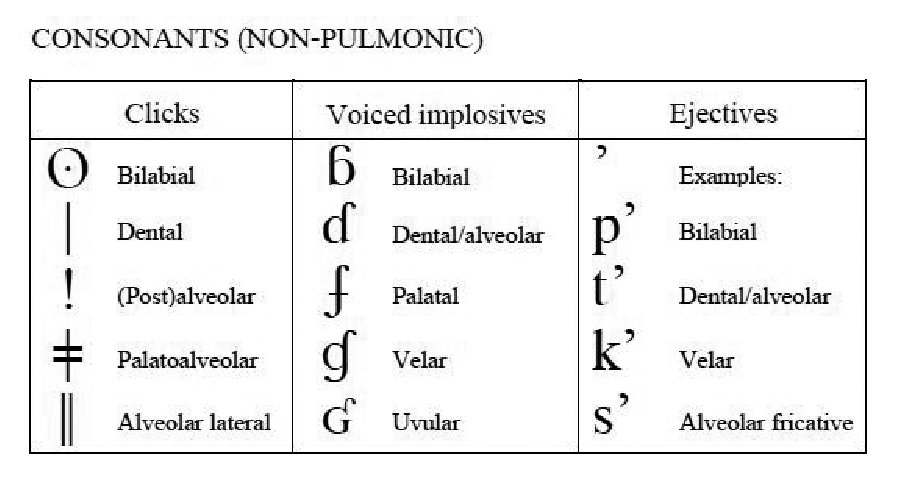
\includegraphics[scale=0.45]{material/04ipaconsonantnonpulmonic}
%		\caption{Konsonanten (Nicht Pulmonal)}
%		%\label{Zeichen1}
%	\end{figure}
	
	\begin{itemize}
		\item \textbf{VIDEO:} \href{run:material/04namaclicks.mp4}{!Nama Clicks}
	\end{itemize}
			
\end{frame}


%%%%%%%%%%%%%%%%%%%%%%%%%%%%%%%%%%%
\begin{frame}
\frametitle{Vokale im IPA-Alphabet: das Vokalviereck}

%	\begin{figure}[H]
%		\centering
%		
%		\includegraphics[scale=0.27]{material/04ipavowelwikicommons}
%		\caption{Vokale}
%		%old picture
%		%\includegraphics[scale=0.45]{material/04ipavowel}
%		%\caption{Vokale}
%		%\label{Zeichen1}
%	\end{figure}


\centerline{
	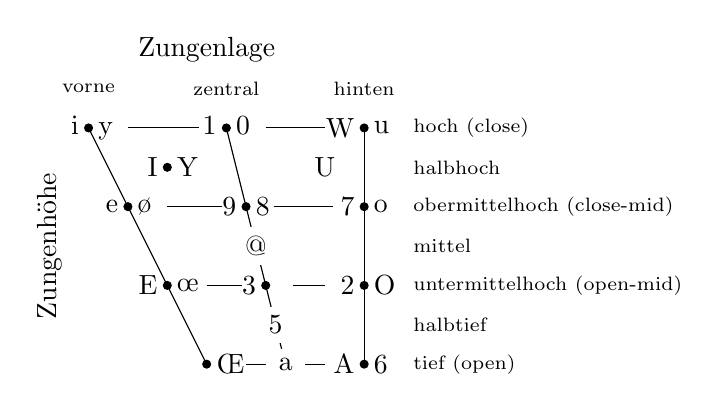
\begin{tikzpicture}
	\draw[fill] (0,0) circle [radius=0.05];
	\draw[fill] (-0.5,1) circle [radius=0.05];
	\draw[fill] (-1,2) circle [radius=0.05];
	\draw[fill] (-1.5,3) circle [radius=0.05];
	\draw[black] (0.5,0)--(0.75,0);
	\draw[black] (1.25,0)--(1.5,0);
	\draw[fill] (2,0) circle [radius=0.05];
	\draw[fill] (2,1) circle [radius=0.05];
	\draw[fill] (2,2) circle [radius=0.05];
	\draw[fill] (2,3) circle [radius=0.05];
	\draw[fill] (0.25,3) circle [radius=0.05];
	\draw[black] (0.25,3)--(1,0);
	\draw[black] (-0.1,3)--(-1,3);
	\draw[black] (0.75,3)--(1.5,3);
	\draw[fill] (0.5,2) circle [radius=0.05];
	\draw[fill] (0.75,1) circle [radius=0.05];
	\node[right] at (0.25,3){\strut \textipa{0}};
	\node[left] at (0.25,3){\strut \textipa{1}};
	\node at (0,4){Zungenlage};
	\node [rotate=90] at (-2,1.5){Zungenhöhe};
	\node at (-1.5,3.5){{\scriptsize vorne}};
	\node at (0.25,3.5){\scriptsize zentral};
	\node at (2,3.5){{\scriptsize hinten}};
	\node[right] at (2.5,3){\scriptsize hoch (close)};
	\node[right] at (2.5,2.5){\scriptsize halbhoch};
	\node[right] at (2.5,2){\scriptsize obermittelhoch (close-mid)};
	\node[right] at (2.5,1.5){\scriptsize mittel};
	\node[right] at (2.5,1){\scriptsize untermittelhoch (open-mid)};
	\node[right] at (2.5,0.5){\scriptsize halbtief};
	\node[right] at (2.5,0){\scriptsize tief (open)};
	\node[left] at (2,3){\textipa{W}};
	\node[right] at (2,3){\textipa{u}};
	\node at (1.5,2.5){\textipa{U}};
	\node[left] at (2,2){\textipa{7}};
	\node[right] at (2,2){\textipa{o}};
	\node[left] at (2,1){\textipa{2}};
	\node[right] at (2,1){\textipa{O}};
	\node[right] at (2,0){\textipa{6}};
	\node[left] at (2,0){\textipa{A}};
	\draw[black] (2,0)--(2,3);
	\node[left] at (0.5,2){\textipa{9}};
	\node[right] at (0.5,2){\textipa{8}};
	\node[rectangle,fill=white] at (0.625,1.5){\textipa{@}};
	\node[left] at (0.75,1){\textipa{3}};
	\node[right] at (0.75,1){\textipa{\textcloserevepsilon}};
	\node[rectangle,fill=white] at (0.875,0.5){\textipa{5}};
	\node[rectangle,fill=white] at (1,0){\textipa{a}};
	\node[right] at (-1.5,3){\strut \textipa{y}};
	\node[left] at (-1.5,3){\strut \textipa{i}};
	\node[left] at (-0.5,2.5){\textipa{I}};
	\node[right] at (-0.5,2.5){\textipa{Y}};
	\draw[fill] (-0.5,2.5) circle [radius=0.05];
	\node[right] at (-1,2){\textipa{\o}};
	\node[left] at (-1,2){\textipa{e}};
	\node[right] at (-0.5,1){\textipa{\oe}};
	\node[left] at (-0.5,1){\textipa{E}};
	\node[right] at (0,0){\textipa{\OE}};
	\draw[black] (0,0)--(-1.5,3);
	\draw[black] (-0.5,2)--(0.2,2);
	\draw[black] (0.85,2)--(1.6,2);
	\draw[black] (0,1)--(0.45,1);
	\draw[black] (1.1,1)--(1.5,1);
	\end{tikzpicture}
}
        
        Vokale links des Punktes sind ungerundet,\\
        die rechts sind gerundet.

%=======
%	\begin{figure}[H]
%		\centering
%		
%		\includegraphics[scale=0.27]{material/04ipavowelwikicommons}
%%		\caption{Vokale}
%		%old picture
%		%\includegraphics[scale=0.45]{material/04ipavowel}
%		%\caption{Vokale}
%		%\label{Zeichen1}
%	\end{figure}
	
\end{frame}


%%%%%%%%%%%%%%%%%%%%%%%%%%%%%%%%%%%
\begin{frame}
\frametitle{Vokale im Deutschen}

\noindent
\begin{minipage}{.55\textwidth}
	\centerline{
	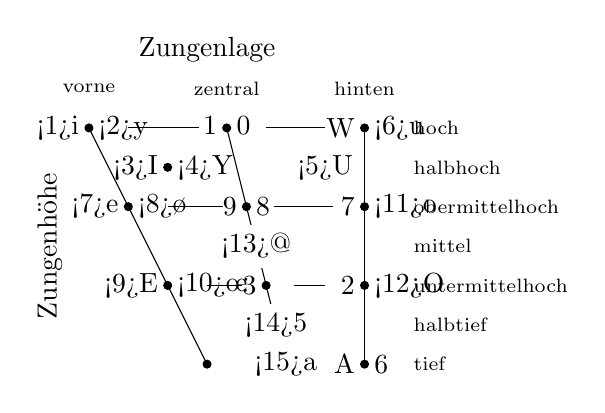
\begin{tikzpicture}
	\draw[fill] (0,0) circle [radius=0.05];
	\draw[fill] (-0.5,1) circle [radius=0.05];
	\draw[fill] (-1,2) circle [radius=0.05];
	\draw[fill] (-1.5,3) circle [radius=0.05];
	\draw[black] (0.5,0)--(0.75,0);
	\draw[black] (1.25,0)--(1.5,0);
	\draw[fill] (2,0) circle [radius=0.05];
	\draw[fill] (2,1) circle [radius=0.05];
	\draw[fill] (2,2) circle [radius=0.05];
	\draw[fill] (2,3) circle [radius=0.05];
	\draw[fill] (0.25,3) circle [radius=0.05];
	\draw[black] (0.25,3)--(1,0);
	\draw[black] (-0.1,3)--(-1,3);
	\draw[black] (0.75,3)--(1.5,3);
	\draw[fill] (0.5,2) circle [radius=0.05];
	\draw[fill] (0.75,1) circle [radius=0.05];
	\node[right] at (0.25,3){\strut \textipa{0}};
	\node[left] at (0.25,3){\strut \textipa{1}};
	\node at (0,4){Zungenlage};
	\node [rotate=90] at (-2,1.5){Zungenhöhe};
	\node at (-1.5,3.5){{\scriptsize vorne}};
	\node at (0.25,3.5){\scriptsize zentral};
	\node at (2,3.5){{\scriptsize hinten}};
	\node[right] at (2.5,3){\scriptsize hoch};
	\node[right] at (2.5,2.5){\scriptsize halbhoch};
	\node[right] at (2.5,2){\scriptsize obermittelhoch};
	\node[right] at (2.5,1.5){\scriptsize mittel};
	\node[right] at (2.5,1){\scriptsize untermittelhoch};
	\node[right] at (2.5,0.5){\scriptsize halbtief};
	\node[right] at (2.5,0){\scriptsize tief};
	\node[left] at (2,3){\textipa{W}};
	\node[right] at (2,3){\alertred{\alertgreen<6>{\textipa{u}}}};
	\node at (1.5,2.5){\alertred{\alertgreen<5>{\textipa{U}}}};
	\node[left] at (2,2){\textipa{7}};
	\node[right] at (2,2){\alertred{\alertgreen<11>{\textipa{o}}}};
	\node[left] at (2,1){\textipa{2}};
	\node[right] at (2,1){\alertred{\alertgreen<12>{\textipa{O}}}};
	\node[right] at (2,0){\textipa{6}};
	\node[left] at (2,0){\textipa{A}};
	\draw[black] (2,0)--(2,3);
	\node[left] at (0.5,2){\textipa{9}};
	\node[right] at (0.5,2){\textipa{8}};
	\node[rectangle,fill=white] at (0.625,1.5){\alertred{\alertgreen<13>{\textipa{@}}}};
	\node[left] at (0.75,1){\textipa{3}};
	\node[right] at (0.75,1){\textipa{\textcloserevepsilon}};
	\node[rectangle,fill=white] at (0.875,0.5){\alertred{\alertgreen<14>{\textipa{5}}}};
	\node[rectangle,fill=white] at (1,0){\alertred{\alertgreen<15>{\textipa{a}}}};
	\node[right] at (-1.5,3){\alertred{\alertgreen<2>{\strut \textipa{y}}}};
	\node[left] at (-1.5,3){\alertred{\alertgreen<1>{\strut \textipa{i}}}};
	\node[left] at (-0.5,2.5){\alertred{\alertgreen<3>{\textipa{I}}}};
	\node[right] at (-0.5,2.5){\alertred{\alertgreen<4>{\textipa{Y}}}};
	\draw[fill] (-0.5,2.5) circle [radius=0.05];
	\node[right] at (-1,2){\alertred{\alertgreen<8>{\textipa{\o}}}};
	\node[left] at (-1,2){\alertred{\alertgreen<7>{\textipa{e}}}};
	\node[right] at (-0.5,1){\alertred{\alertgreen<10>{\textipa{\oe}}}};
	\node[left] at (-0.5,1){\alertred{\alertgreen<9>{\textipa{E}}}};
	\node[right] at (0,0){\textipa{\textscoelig }};
	\draw[black] (0,0)--(-1.5,3);
	\draw[black] (-0.5,2)--(0.2,2);
	\draw[black] (0.85,2)--(1.6,2);
	\draw[black] (0,1)--(0.45,1);
	\draw[black] (1.1,1)--(1.5,1);
	\end{tikzpicture}
}

\medskip

Deutsche Vokale sind \alt<handout>{unterstrichen.}{rot.}
\end{minipage}
\hfill
\begin{minipage}{.42\textwidth}
	\begin{itemize}
	\item Liege [\textipa{li:g@}]\pause,  Lüge [\textipa{ly:g@}]\pause
	\item Kiste [\textipa{kIst@}]\pause,  Küste [\textipa{kYst@}]\pause
	\item muss [\textipa{mUs}]\pause,   Mus   [\textipa{mu:s}]\pause
	\item Wege  [\textipa{ve:g@}]\pause,  wöge [\textipa{vø:g@}]\pause
	\item helle [\textipa{hEl@}]\pause,   Hölle [\textipa{hœl@}]\pause
	\item Ofen  [\textipa{o:f@n}]\pause,  offen [\textipa{Of@n}]\pause
	\item geben [\textipa{ge:b@n}]\pause, Lehrer [\textipa{le:K5}]\pause
	\item Lab   [\textipa{la:p}]
	\end{itemize}
\end{minipage}
\end{frame}


%%%%%%%%%%%%%%%%%%%%%%%%%%%%%%%%%%%
\begin{frame}
\frametitle{Suprasegmentalia}

\begin{tabular}{l|p{6cm}|p{3cm}}
\textbf{Zeichen} &	\textbf{Erklärung} & \textbf{Beispiel} \\
\hline
\alertred{\textipa{\textprimstress}} & Hauptbetonung &[\textipa{Pa.po.\textprimstress te:.k@}]\\

\alertred{\textipa{\textsecstress}} & Nebenbetonung & [\textipa{\textprimstress ba:n.ho:fs.\textsecstress plE:.n@}]\\

\alertred{\textipa{:}} & lang & [\textipa{ba:n}] (vs. [\textipa{ban}])\\

\textipa{;} & halblang & \\

\textipa{\u{}} \textipa{\alertred{\textsubarch{ }}} & extra-kurz/unsilbischer Vokal & [\textipa{stu:d\textsubarch{i}@}], [\textipa{stu:d\u{i}@}]\\

\textipa{\textvertline} & untergeordnete Intonationsgruppe &\\

\textipa{\textdoublevertline} &	übergeordnete Intonationsgruppe & \\

\alertred{\textipa{.}} & Silbengrenze & [\textipa{\textprimstress zIl.bEn.\textsecstress gKEn.\t{ts}@}]\\

\alertred{\textipa{\t{}}} & Doppelartikulation & [\textipa{P\t{aU}to}],  [\textipa{nE\t{ts}}] \\

\alertred{\textipa{\.}} & Silbengelenkmarker & \textipa{[kO\.m@]}\\

\alertred{\textipa{\textsyllabic{ }}} & silbische Konsonanten & \textipa{[kUm.p\textsyllabic{l}]}\\
\end{tabular}

\medskip

Die rot markierten Zeichen werden Sie häufiger in diesem und in zukünftigen Seminaren sehen.

\end{frame}


%%%%%%%%%%%%%%%%%%%%%%%%%%%%%%%%%%%
%%%%%%%%%%%%%%%%%%%%%%%%%%%%%%%%%%%
\subsection{Artikulatorische Phonetik}

%% MyP: Contents
\iftoggle{sectoc}{
	\frame{
		%\begin{multicols}{2}
		\frametitle{~}
		\tableofcontents[currentsubsection,subsubsectionstyle=hide]
		%\end{multicols}
	}
}

%% StM: Contents
\iftoggle{gliederung}{
\outline{

\begin{itemize}

\item Einführung
\item Bereiche der Phonetik
\item  Methodik
\item  Probleme der Phonetik
\item  IPA-Alphabet
\item \blaubf{Artikulatorische Phonetik}
\begin{itemize}
\item Konsonanten
\item Konsonantenklassiffikation
\item Vokale
  \item Vokalklassiffikation
\item Vokalviereck
\item Monophthong, Diphthong, Triphthong
    \end{itemize}
\item Übungen
  
  \end{itemize}
	}
}


%%%%%%%%%%%%%%%%%%%%%%%%%%%%%%%%%%%
\begin{frame}{Artikulatorische Phonetik: Initiator, Generator, Modifikator}

Mehrere Körperteile sind für Erzeugung von Schall nötig:
		
\begin{itemize}
	\item \textbf{Initiator}:\\
	die Lunge \ras (Atmung) erzeugt Luftstrom
	
	\item \textbf{Generator}:\\
	der Kehlkopf (Larynx) mit den Stimmbändern \ras\\
	Luftstrom wird in Schwingung versetzt (Phonation)

	\item \textbf{Frequenz}: Häufigkeit, mit der die Stimmlippen schwingen\\
	\medskip
	Frequenz bestimmt die Tonhöhe:
	
	\begin{itemize}
		\item bei Frauen ung. 230 Hz
		\item bei Männern 120 Hz 
		\item bei Säuglingen 400 Hz
	\end{itemize}

\end{itemize}

\textbf{VIDEO:} \href{run:material/04TransNasalEndoscopy.mp4}{Trans-Nasal Endoscopy}


\end{frame}


%%%%%%%%%%%%%%%%%%%%%%%%%%%%%%%%%%%
\begin{frame}{Artikulatorische Phonetik: Initiator, Generator, Modifikator}

Mehrere Körperteile sind für Erzeugung von Schall nötig:

\begin{itemize}
	\item \textbf{Modifikator}: Rachen-, Mund- und Nasenraum mit den verschiedenen Sprechwerkzeugen (Zunge, Lippen, weicher Gaumen)

\medskip
	
	Unterschiedliche Stellung der Artikulationsorgane verändert den Rohschall des Kehlkopfs zu den wohlunterschiedenen Lauten (Artikulation im engeren Sinne).
\end{itemize}
	
\end{frame}


%%%%%%%%%%%%%%%%%%%%%%%%%%%%%%%%%%%
%%%%%%%%%%%%%%%%%%%%%%%%%%%%%%%%%%%
\subsubsection{Konsonanten}
%%% MyP: Contents
%\iftoggle{sectoc}{
%	\frame{
%		%\begin{multicols}{2}
%		\frametitle{~}
%		\tableofcontents[currentsubsubsection]
%		%\end{multicols}
%	}
%}
%%%%%%%%%%%%%%%%%%%%%%%%%%%%%%%%%%%
\begin{frame}{Konsonanten}

	\begin{itemize}
		\item auch genannt: Mitlaute
		
		\item Die Artikulationsorgane bilden eine \textbf{geräuschverursachende Enge} oder einen \textbf{Verschluss} im Ansatzrohr, \dash die Luft wird oberhalb der Stimmritze (Glottis) zwischen den Stimmbändern behindert.
	\end{itemize}
	
\end{frame}


%%%%%%%%%%%%%%%%%%%%%%%%%%%%%%%%%%%
\begin{frame}
\frametitle{Sagittalschnitt}

\begin{minipage}{0.48\textwidth}
	\begin{figure}
	\centering
	\includegraphics[scale=0.32]{material/04phonoatonomy}
	\caption{Sagittalschnitt}
	\end{figure}
\end{minipage}\hfill
\begin{minipage}{0.4\textwidth}
	A -- Nasenraum\\
	B -- Zahndamm \emph{Alveolen}\\
	C -- (Ober)Lippe \\
	D -- (obere) Zähne\\
	E -- Zungenspitze \emph{Apex}\\
	F -- Kehlkopf \emph{Larynx}\\
	G -- Stimmlippen \emph{Glottis}\\
	H -- harter Gaumen \emph{Palatum}\\
	I -- Zungenrücken \emph{Dorsum}\\
	J -- Gaumensegel \emph{Velum}\\
	K -- Zäpfchen \emph{Uvula}\\
	L -- Luftröhre\\ 
	M -- Speiseröhre
\end{minipage}
	
%	\begin{figure}[H] %%altes Bild%%
%		\centering
%		
%		\includegraphics[scale=0.65]{material/04sagitalschnittaltmann}
%		\caption{Sagitalschnitt \citep{Altmann&Co07a}}
%		%\label{Zeichen1}
%	\end{figure}
	
\end{frame}


%%%%%%%%%%%%%%%%%%%%%%%%%%%%%%%%%%%
%%%%%%%%%%%%%%%%%%%%%%%%%%%%%%%%%%%
\subsubsection{Konsonantenklassifikation}
%%% MyP: Contents
%\iftoggle{sectoc}{
%	\frame{
%		%\begin{multicols}{2}
%		\frametitle{~}
%		\tableofcontents[currentsubsubsection]
%		%\end{multicols}
%	}
%}
%%%%%%%%%%%%%%%%%%%%%%%%%%%%%%%%%%%
\begin{frame}{Konsonantenklassifikation: Stimmbeteiligung}

	\begin{itemize}
		\item \textbf{Stimmbeteiligung} (Stimmhaftigkeit): Schwingungszustand der Stimmbänder
		
		\begin{itemize}
			
			\item \textbf{stimmlos} \ras weit auseinander stehende Stimmbänder
			
			\item \textbf{stimmhaft} \ras eng beieinander stehende Stimmbänder
			
			\ea \textipa{[ p ]} vs. \textipa{[ b ]}
			\z

			
			\item \textbf{Aspiration} (Behauchung):\par
				Glottis während der Verschlussphase ist weit gespreizt und schwingt mit.

			\ea \textipa{[ \super h ]}
			\z

                        \textbf{VIDEO:} \href{run:material/02-aspiration.mp4}{Aspiration}
		\end{itemize}

	\end{itemize}
	
\end{frame}


%%%%%%%%%%%%%%%%%%%%%%%%%%%%%%%%%%
\begin{frame}
\frametitle{Übung}
Welche der folgenden Laute sind stimmhaft und welche stimmlos?

\ea \label{ex:02sth}
\textipa{[ d, z, f, v, g, k, P ]}
\z

\end{frame}


%%%%%%%%%%%%%%%%%%%%%%%%%%%%%%%%%%
\iftoggle{ue-loesung}{
	%%%%%%%%%%%%%%%%%%%%%%%%%%%%%%%%%%
%% UE 2 - 02 Phonetik
%%%%%%%%%%%%%%%%%%%%%%%%%%%%%%%%%%

\begin{frame}
\frametitle{Übung -- Lösung}

Welche der folgenden Laute sind stimmhaft und welche stimmlos?

\begin{exe}
\exr{ex:02sth} \textipa{[ d, z, f, v, g, k, P ]}
\end{exe}


\begin{multicols}{2}
	\begin{itemize}
		\item \textbf{stimmhaft:} \alertgreen{\textipa{[ d, z, v, g ]}}
		
		\ea \alertgreen{\textipa{[ d ]}: \ab{Dampf}}
		
		\ex \alertgreen{\textipa{[ z ]}: \ab{Sinn}}
		
		\ex \alertgreen{\textipa{[ v ]}: \ab{Wald}}
		
		\ex \alertgreen{\textipa{[ g ]}: \ab{ganz}}
		
		\z 
	\end{itemize}
	
	\columnbreak \pause
	
	\begin{itemize}
		\item \textbf{stimmlos:} \alertgreen{\textipa{[ f, k, P ]}}
		
		\ea \alertgreen{\textipa{[ f ]}: \ab{Fass}}
		
		\ex \alertgreen{\textipa{[ k ]}: \ab{kalt}}
		
		\ex \alertgreen{\textipa{[ P ]}: \ab{vereisen}}
		
		\z
	\end{itemize}
	
\end{multicols}

\end{frame}


}

%%%%%%%%%%%%%%%%%%%%%%%%%%%%%%%%%%%%
\begin{frame}
\frametitle{Konsonantenklassifikation: Stellung des Gaumensegels}

	\begin{itemize}
		\item \textbf{Stellung des Gaumensegels} (des weichen Gaumens):
		
		\begin{itemize}
			
			\item Nasale Laute (\zB \textipa{ [ m, n ]}) \ras Senkung des weichen Gaumens (Velum)
			
			\item Orale Laute (\zB \textipa{ [ f, a ]}) \ras bei gehobenem Velum
		\end{itemize}
		
		
		\item[] \textbf{LINK:} \href{http://smu-facweb.smu.ca/~s0949176/sammy/}{interaktiver Sagittalschnitt}
	\end{itemize}
	
\end{frame}


%%%%%%%%%%%%%%%%%%%%%%%%%%%%%%%%%%%
\begin{frame}
\frametitle{Konsonantenklassifikation: Artikulationsort (I)}

	\begin{itemize}
	\item \textbf{Artikulationsort} im Vokaltrakt: Ort, an dem die Luft behindert wird
          Unterscheidung nach nicht-beweglichen und beweglichen Artikulatoren

\medskip
		
		\item \textbf{Nicht-bewegliche} Artikulatoren (passiver Artikulator, Artikulationsort im engeren Sinne):
			
		\begin{itemize}
			\item die oberen Zähne \ras \textbf{dental}
			
			\item die Alveolen (Knochendamm hinter den oberen Zähnen) \ras \textbf{alveolar}
			
			\item der harte Gaumen (Palatum) \ras \textbf{palatal}
		\end{itemize}
		
	\end{itemize}
	
\end{frame}


%%%%%%%%%%%%%%%%%%%%%%%%%%%%%%%%%%%
\begin{frame}
\frametitle{Konsonantenklassifikation: Artikulationsort (II)}

\begin{itemize}
	\item \textbf{Bewegliche} Artikulatoren (aktiver Artikulator, Artikulationsorgan):
			
	\begin{itemize}
		
		\item weicher Gaumen (Velum) \ras \textbf{velar}
		
		\item das Zäpfchen (Uvula) \ras \textbf{uvular}
		
		\item Lippen \ras \textbf{labial}
		
		\item Unterkiefer
		
		\item Zunge
	\end{itemize}

\end{itemize}

\end{frame}


%%%%%%%%%%%%%%%%%%%%%%%%%%%%%%%%%%%
\begin{frame}
\frametitle{Konsonantenklassifikation: Artikulationsort (III)}

		\begin{itemize}
			\item Bei der Artikulation mit der \textbf{Zunge} bildet man Untergruppen nach dem \textbf{beteiligten Zungenteil}:
			
			\begin{itemize}
				\item \textbf{koronal}: mit dem vorderen Teil der Zunge
	
				\begin{itemize}
					\item \textbf{apikal}: mit der Zungenspitze
					
					\item \textbf{laminal}: mit dem Zungenblatt (mittlerer Teil der Zunge)				
				\end{itemize}
	
				\ea \textipa{[ t, d, l, n, s, z, S, Z ]}
				\z

\pause

				\item \textbf{dorsal}: mit dem hinteren Teil der Zunge

				\ea \textipa{[ \c{c}, j, g, k, x, N, \textscr, K ]}
				\z

			\end{itemize}

					
		\item[] \textbf{LINK:} \href{http://smu-facweb.smu.ca/~s0949176/sammy/}{Interaktiver Sagittalschnitt}

		\end{itemize}
		
\end{frame}


%%%%%%%%%%%%%%%%%%%%%%%%%%%%%%%%%%%
\begin{frame}
\frametitle{Konsonantenklassifikation: Artikulationsart}

	\begin{block}{Artikulationsart}
	(auch Artikulationsmodus)\\
	Art der Behinderung des Luftstroms durch die Artikulationsorgane
	\end{block}	

\end{frame}


%%%%%%%%%%%%%%%%%%%%%%%%%%%%%%%%%%%
\begin{frame}
\frametitle{Artikulationsart: Plosive}

\begin{itemize}
			\item \textbf{Plosive} (Verschlusslaute, Explosivlaute, stops): totaler oraler Verschluss mit anschließender plötzlicher Lösung des Verschlusses\\
				Das Velum bleibt dabei in angehobener Position,\par
				so dass die Luft durch den Mundraum strömt.

			\ea \textipa{[ p, b, t, d, k, g, P ]}
			\z
			
			Der \textbf{Glottalverschluss} (Knacklaut) \textipa{[ P ]} entsteht durch plötzliches Öffnen der Stimmritze und kommt im Deutschen vor anlautendem Vokal eines Wortes und vor anlautendem Vokal in einer betonten Silbe vor.
		
	\end{itemize}
	
\end{frame}


%%%%%%%%%%%%%%%%%%%%%%%%%%%%%%%%%%%
\begin{frame}
\frametitle{Artikulationsart: Frikative}

		\begin{itemize}
			\item \textbf{Frikative} (Reibelaute, Spiranten): Verengung zweier Sprechorgane,\\
                          Luftstrom strömt durch die Verengung, es entsteht ein Reibegeräusch.

			\ea \textipa{[ f, v, s, z, S, Z, \c{c}, x, h, K ]}
			\z

\pause 
			
			\begin{itemize}
				\item \textbf{Sibilanten} (Zischlaut):\par
					Unterklasse der Frikative mit intensivem, hochfrequentem Geräuschanteil.

				\ea \textipa{[ s, z, S ]}
				\z

		\end{itemize}
		
	\end{itemize}
	
\end{frame}


%%%%%%%%%%%%%%%%%%%%%%%%%%%%%%%%%%%
\begin{frame}
%\frametitle{Konsonantenklassifikation}
\frametitle{Artikulationsart: Affrikaten}

		\begin{itemize}
			\item \textbf{Affrikaten}: Plosive, die in Frikative übergehen, wobei die Verschlussphase und die Frikativphase dieselbe (oder annähernd dieselbe) Artikulationsstelle haben; d.\,h. sie sind \textbf{homorgan}.

			\ea \textipa{[ \texttoptiebar{pf}, \texttoptiebar{ts}, \texttoptiebar{tS}, \texttoptiebar{dZ} ]} %\textipa{ \t{aUI}}
			\z

			\begin{itemize}
				\item Per Definition gehören der plosive und der frikative Laut einer Affrikaten \textbf{zum selben Morphem} (die kleinste bedeutungstragende Einheit). Daraus ergibt sich:

				\ea \textipa{[ \t{ts} ]} in \ab{Blitz} \ras Affrikate
				\z
				
				\ea \textipa{[ ts ]} in \ab{Monats} \ras keine Affrikate
				\z

			\end{itemize}
		
		
		\item Plosive, Frikative und Affrikaten \ras \textbf{Obstruenten}
	\end{itemize}
	
\end{frame}


%%%%%%%%%%%%%%%%%%%%%%%%%%%%%%%%%%%
\begin{frame}
\frametitle{Artikulationsart: Vibranten}

		\begin{itemize}
			\item \textbf{Vibranten} (trills): schnelle Folge oraler Verschlüsse
			\begin{itemize}
				
				\item Artikulationsstellen für Vibranten sehr eingeschränkt: nur bilabial, alveolar oder uvular
				
				\item Der alveolare Vibrant \textipa{[ r ]} (das sog. Zungenspitzen-R) kommt in vielen süddeutschen Varietäten vor.
				
				\item Der uvulare Vibrant \textipa{[ \textscr\ ]} (das gerollte Zäpfchen-R) ist eine häufige Realisierung des Deutschen \ab{r}.
			\end{itemize}
			 
	\end{itemize}
	
\end{frame}


%%%%%%%%%%%%%%%%%%%%%%%%%%%%%%%%%%%
\begin{frame}
\frametitle{Artikulationsart: Approximanten}

		\begin{itemize}
			\item \textbf{Approximanten} (Öffnungslaute): Enge im Ansatzrohr (wie Frikative)\\
			Bei Approximanten gibt es nicht so eine große Nähe zwischen Artikulator und Artikulationsstelle \ras kein Reibegeräusch
			
			 Zwei Unterklassen:
			
			\begin{itemize}
				
				\item \textbf{Laterale}: Verschluss in der Mundhöhlenmitte, Luft entweicht seitlich [~\textipa{l}~]
				
				\item \textbf{Gleitlaute} (zentral): zentrale Verengung, aber weiter als bei Frikativen [~\textipa{w}~].\\
				(Manchmal wird [~\textipa{j}~] auch zu den Gleitlauten gezählt,\\
                                  da die Verengung weiter als bei anderen Frikativen ist. Dies ist jedoch strittig.)
			\end{itemize}
			
		\end{itemize}	

\end{frame}


%%%%%%%%%%%%%%%%%%%%%%%%%%%%%%%%%%%
\begin{frame}
%\frametitle{Konsonantenklassifikation}
\frametitle{Artikulationsart: Nasale}
		\begin{itemize}
			\item \textbf{Nasale}: totaler oraler Verschluss (wie Plosive).\\
				Luft entweicht durch die Nase durch Senken des Velums.
			 
			 \ea \textipa{[ m, n, N ]}
			 \z
		
		\item Vibranten, Approximanten (Laterale und Gleitlaute), Nasale und Vokale (auch die hier nicht behandelten \gqq{geschlagenen Laute} wie das span. \textipa{[~R~]}) gehören zur Gruppe der \textbf{Sonoranten}, da die Luft ungehindert ausströmen kann. Sonoranten sind \textbf{immer} stimmhaft!
		
		\item Die Klasse der l-Laute und r-Laute werden auch zu den sog. \textbf{Liquiden} zusammengefasst (im Dt. \textipa{[ l, r, \textscr ]})
	\end{itemize}

	
\end{frame}


%%%%%%%%%%%%%%%%%%%%%%%%%%%%%%%%%%%
\begin{frame}
	\frametitle{Konsonantenklassifikation: Zusammenfassung I}
	
\begin{figure}
	\centering
	
\scalebox{.85}{
\begin{forest}
	sm edges
	[Konsonanten
		[\textbf{Obstruenten}\\{[}$-$son{]}
			[Frikative\\{[}$+$kont{]}
				[{[}$+$sth{]} [\textipa{v z Z}, no edge] ]
				[{[}$-$sth{]} [\textipa{f s S \c{c}}, no edge] ]
			]
			[Plosive\\{[}$-$kont{]}
				[{[}$+$sth{]} [\textipa{b d g}, no edge] ]
				[{[}$-$sth{]} [\textipa{p t k}, no edge] ]
			]
		]
		[\textbf{Sonoranten}\\{[}$-$son{]}
			[Liquide\\{[}$-$nas{]}
				[Laterale\\{[}$+$lat{]} [\textipa{l}, no edge] ]
				[Vibranten\\{[}$-$lat{]} [\textipa{r  R K}, no edge] ]
			]
			[Nasale\\{[}$+$nas{]} [\textipa{m n N}, no edge] ]
		]
	]
\end{forest}
}

\end{figure}

Zur Gruppe der \textbf{Sonoranten} zählen alle Konsonanten, bei denen die Luft \textbf{ungehindert} ausströmen kann. Sie sind \textbf{immer stimmhaft}.

Obstruenten können stimmhaft oder auch stimmlos sein.
	
\end{frame}


%%%%%%%%%%%%%%%%%%%%%%%%%%%%%%%%%%%
\begin{frame}
	\frametitle{Konsonantenklassifikation: Zusammenfassung II}

	\begin{itemize}
		\item Für die \textbf{Differenzierung der deutschen Konsonanten} sind hauptsächlich 3 Merkmale wichtig:
		
		\begin{itemize}
			
			\item Stimmbeteiligung
			\item Artikulationsort
			\item Artikulationsart
		\end{itemize}
	\end{itemize}

\textbf{LINK}: \href{http://www.ipachart.com/}{Interactive IPA chart}

\end{frame}


%%%%%%%%%%%%%%%%%%%%%%%%%%%%%%%%%%
\begin{frame}

\frametitle{Übung}

\begin{itemize}
	\item[] Beschreiben Sie die Konsonanten in den folgenden Wörtern und geben Sie die entsprechenden phonetischen Symbole an:
	
	\begin{enumerate}
		\item Busch
		\item malen
		\item Maus
		\item Achtung
		\item Genie
		\item zirpen
		\item wichtig
		\item Wald
	\end{enumerate}
	
\end{itemize}
\end{frame}


%%%%%%%%%%%%%%%%%%%%%%%%%%%%%%%%%%%
\iftoggle{ue-loesung}{
	%%%%%%%%%%%%%%%%%%%%%%%%%%%%%%%%%%
%% UE 3 - 02 Phonetik
%%%%%%%%%%%%%%%%%%%%%%%%%%%%%%%%%%

\begin{frame}
\frametitle{Übung -- Lösung}

\begin{table}
\scalebox{.9}{
	\begin{tabular}{llp{9cm}}
		1. Busch & \only<2->{[\textipa{bUS}]} & \only<3->{\textipa{b}: bilabialer, stimmhafter Plosiv; \textipa{S}:~postalveolarer, stimmloser Frikativ} \\
		
		2. malen & \only<4->{[\textipa{\textprimstress ma:l@n}]} & \only<5->{\textipa{m}:~bilabialer, stimmhafter Nasal; \textipa{n}:~alveolarer, stimmhafter Nasal, \textipa{l}:~alveolar, stimmhafter Lateral} \\
		
		3. Maus & \only<6->{[\textipa{m\texttoptiebar{aU}s}]} & \only<7->{\textipa{m}:~s.\,o.; \textipa{s}:~stimmloser, alveolarer Frikativ} \\
		
		4. Achtung & \only<8->{[\textipa{\textprimstress PaXtU\ng}]} & \only<9->{\textipa{P}:~glottaler, stimmloser Plosiv; \textipa{X}:~velarer, stimmloser Frikativ; \textipa{t}:~alveolarer, stimmloser Plosiv \textipa{\ng}: velarer, stimmhafter Nasal} \\

		5. Genie & \only<10->{[\textipa{Ze:\textprimstress ni:}]} & \only<11->{\textipa{Z}: postalveolarer, stimmhafter Frikativ, \textipa{n}:~s.\,o.} \\                
		                                                                                  
		6. zirpen & \only<12->{[\textipa{\texttoptiebar{ts}IKp@n}]} & \only<13->{\textipa{\texttoptiebar{ts}}: alveolare, stimmlose Affrikate; \textipa{K}:~uvularer, stimmhafter Frikativ; \textipa{p}:~bilabialer, stimmloser Plosiv; \textipa{n}: s.\,o.} \\

		7. wichtig & \only<14->{[\textipa{\textprimstress vI\c{c}tI\c{c}}]} & \only<15->{\textipa{v}: labiodentaler, stimmhafter Frikativ; \textipa{\c{c}}: palataler, stimmloser Frikativ \textipa{t}: s.\,o.} \\

		8. Wald & \only<16->{[\textipa{valt}]} & \only<17->{\textipa{v, l, t}: s.\,o.}
\end{tabular}
}
\end{table}

\end{frame}

}
%%%%%%%%%%%%%%%%%%%%%%%%%%%%%%%%%%%

%%%%%%%%%%%%%%%%%%%%%%%%%%%%%%%%%%
%%%%%%%%%%%%%%%%%%%%%%%%%%%%%%%%%%
\subsubsection{Vokale}

%%% MyP: Contents
%\iftoggle{sectoc}{
%	\frame{
%		%\begin{multicols}{2}
%		\frametitle{~}
%		\tableofcontents[currentsubsubsection]
%		%\end{multicols}
%	}
%}
%%%%%%%%%%%%%%%%%%%%%%%%%%%%%%%%%%%
\begin{frame}{Vokale}

	\begin{itemize}
		\item \textbf{Vokale} (Selbstlaute) sind Laute, bei deren Artikulation die Luft ungehindert durch den Mundraum strömen kann (deswegen gehören sie zu den \textbf{Sonoranten}).
		
		\item Vokale sind \idR immer \textbf{stimmhaft}.
		
		\item Es ist umstritten, ob der sog. Schwa-Laut im Dt. \textipa{[ @ ]} stimmhaft
                  ist.\\
                  Auch im Japanischen soll es stimmlose Vokale geben.
	\end{itemize}
	
\end{frame}


%%%%%%%%%%%%%%%%%%%%%%%%%%%%%%%%%%%
%%%%%%%%%%%%%%%%%%%%%%%%%%%%%%%%%%%
\subsubsection{Vokalklassifikation}
%%% MyP: Contents
%\iftoggle{sectoc}{
%	\frame{
%		%\begin{multicols}{2}
%		\frametitle{~}
%		\tableofcontents[currentsubsubsection]
%		%\end{multicols}
%	}
%}
%%%%%%%%%%%%%%%%%%%%%%%%%%%%%%%%%%%

\begin{frame}{Vokalklassifikation I}

	\begin{itemize}
		\item \textbf{Zungenhöhe} (Vokalhöhe): Grad der Zungenhebung in Richtung Gaumen

		\ea hoch: \textipa{[ i: ]}, mittel: \textipa{[ o: ]}, tief: \textipa{[ a: ]} bzw. geschlossen, halboffen, offen
		\z

\pause 

		\item \textbf{Zungenlage} (Vokaltiefe): angehobener Teil der Zunge

		\ea vorne: \textipa{[ i: ]}, zentral: \textipa{[ a: ]}, hinten: \textipa{[ u: ]}
		\z

\pause 

		\item \textbf{Lippenrundung}: Art der Lippenöffnung

		\ea gerundet: \textipa{[ o: ]}, ungerundet: \textipa{[ i: ]}
		\z

		\bigskip
 

 	\item Lesen Sie folgende Wörter mit \textbf{gerundeten} und mit \textbf{gespreizten} Lippen:
	\ea 
	\ea Bühne, rühmen, Dünen, Stiele, Trieb, Möhre, Herd, Hefe, kennen

\pause 	

	\ex  Biene, Riemen, dienen, Stühle, trüb, Meere, hört, Höfe, können
	\z  
	\z 
 
\end{itemize}

\end{frame}


%%%%%%%%%%%%%%%%%%%%%%%%%%%%%%%%%%%
\begin{frame}
\frametitle{Vokalklassifikation II}

\begin{itemize}
	\item Gespanntheit:

\begin{description}
	\item[\textbf{Definition 1}] \textipa{[ i:, y:, u:, o: ]} mit \textbf{mehr Muskelspannung} als \textipa{[ I, Y, U, O ]} 
	
	(von der experimentellen Phonetik weder bestätigt noch widerlegt)
	
	\item[\textbf{Definition 2}] \textipa{[ i:, y:, u:, o: ]}  mit \textbf{vorverlagerter Zungenwurzel}


\begin{multicols}{2}

\textbf{gespannt:}
	\ea \textipa{[ i: ]}: \ab{Liege}
	
	\ex \textipa{[ y: ]}: \ab{Lüge}
	
	\ex \textipa{[ u: ]}: \ab{Mus}
	
	\ex \textipa{[ o: ]}: \ab{Ofen}
	
	\z 
	
\columnbreak
	
\textbf{ungespannt:}
	\ea \textipa{[ I ]}: \ab{Kiste}
	
	\ex \textipa{[ Y ]}: \ab{Küste}
	
	\ex \textipa{[ U ]}: \ab{muss}
	
	\ex \textipa{[ O ]}: \ab{offen}
	
	\z
	
\end{multicols}

\end{description}
\end{itemize}
			
\end{frame}		

%%%%%%%%%%%%%%%%%%%%%%%%%%%%%%%%%%%			
			
\begin{frame}
\frametitle{Anmerkungen zur Gespanntheit}
		\begin{itemize}	
			\item i.\,d.\,R. alle tiefen Vokale \ras ungespannt (strittig!)
			\item langer tiefer Vokal \textipa{[ a: ]} \ras gespannt(?)
%		\end{itemize}

	      \item im Deutschen: Korrelation der Gespanntheit mit der Länge

		\ea \textipa{[ m i: t @ ]} vs. \textipa{[ m I t @ ]}
		\z

		\item in Lehnwörtern auch kurze gespannte Vokale

		\ea \textipa{[ P i . d e: ]}
		\z
		
	\end{itemize}
	
\end{frame}


%%%%%%%%%%%%%%%%%%%%%%%%%%%%%%%%%%%
\begin{frame}
\frametitle{Vokalklassifikation III}

	\begin{itemize}
	
		
%\vspace{1em}
		
		\item \textbf{Stellung des Gaumensegels}:
		
		\begin{itemize}
			\item oral
			\item nasal
			
			\item Nasalvokale kommen im Dt. nur in Lehnwörtern vor.

			\eal
			\ex \textipa{[ \~a ]} in \ab{Restaur\textbf{ant}}
			\ex \textipa{[ \~E ]} in \ab{T\textbf{eint}}
			\ex \textipa{[ \~o ]} in \ab{Balk\textbf{on}}
			\ex \textipa{[ \~\oe\ ]} in \ab{in Parf\textbf{um}}
			\zl
		
		\end{itemize}
		
	\end{itemize}
	
\end{frame}


%%%%%%%%%%%%%%%%%%%%%%%%%%%%%%%%%%%
\begin{frame}
\frametitle{Vokalklassifikation: Überblick}

	\begin{itemize}
		\item Für die \textbf{Differenzierung der deutschen nativen Vokale} sind hauptsächlich vier Merkmale wichtig:
		
		\begin{itemize}
			
			\item Zungenhöhe
			
			\item Zungenlage
			
			\item Lippenrundung
			
			\item Gespanntheit (bzw. Länge)
		\end{itemize}
		
	\end{itemize}

\textbf{LINK}: \href{http://www.ipachart.com/}{Interactive IPA chart}
	
\end{frame}


%%%%%%%%%%%%%%%%%%%%%%%%%%%%%%%%%%%
%%%%%%%%%%%%%%%%%%%%%%%%%%%%%%%%%%%
\subsubsection{Vokalviereck}
%%% MyP: Contents
%\iftoggle{sectoc}{
%	\frame{
%		%\begin{multicols}{2}
%		\frametitle{~}
%		\tableofcontents[currentsubsubsection]
%		%\end{multicols}
%	}
%}
%%%%%%%%%%%%%%%%%%%%%%%%%%%%%%%%%%%

\begin{frame}{Vokalviereck}

	\begin{itemize}
		\item Vokale wurden 1920 von Daniel Jones im sog. Vokalviereck angeordnet.
		\item Vokalviereck stellt eine stilisierte Version des Vokalraums dar.
	\end{itemize}

\begin{figure}
	\centering
%\scalebox{.8}{	
	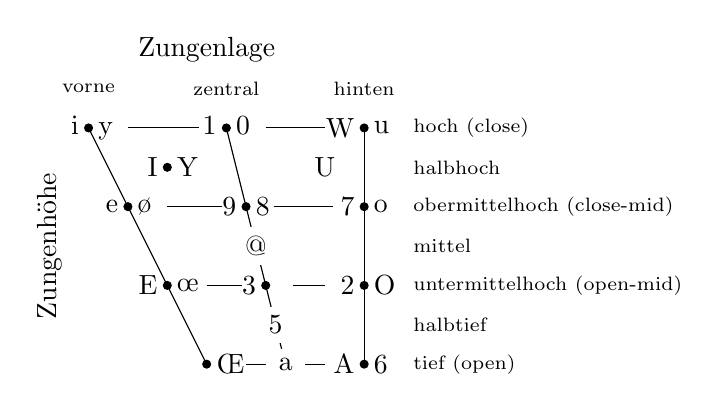
\begin{tikzpicture}
	\draw[fill] (0,0) circle [radius=0.05];
	\draw[fill] (-0.5,1) circle [radius=0.05];
	\draw[fill] (-1,2) circle [radius=0.05];
	\draw[fill] (-1.5,3) circle [radius=0.05];
	\draw[black] (0.5,0)--(0.75,0);
	\draw[black] (1.25,0)--(1.5,0);
	\draw[fill] (2,0) circle [radius=0.05];
	\draw[fill] (2,1) circle [radius=0.05];
	\draw[fill] (2,2) circle [radius=0.05];
	\draw[fill] (2,3) circle [radius=0.05];
	\draw[fill] (0.25,3) circle [radius=0.05];
	\draw[black] (0.25,3)--(1,0);
	\draw[black] (-0.1,3)--(-1,3);
	\draw[black] (0.75,3)--(1.5,3);
	\draw[fill] (0.5,2) circle [radius=0.05];
	\draw[fill] (0.75,1) circle [radius=0.05];
	\node[right] at (0.25,3){\strut \textipa{0}};
	\node[left] at (0.25,3){\strut \textipa{1}};
	\node at (0,4){Zungenlage};
	\node [rotate=90] at (-2,1.5){Zungenhöhe};
	\node at (-1.5,3.5){{\scriptsize vorne}};
	\node at (0.25,3.5){\scriptsize zentral};
	\node at (2,3.5){{\scriptsize hinten}};
	\node[right] at (2.5,3){\scriptsize hoch (close)};
	\node[right] at (2.5,2.5){\scriptsize halbhoch};
	\node[right] at (2.5,2){\scriptsize obermittelhoch (close-mid)};
	\node[right] at (2.5,1.5){\scriptsize mittel};
	\node[right] at (2.5,1){\scriptsize untermittelhoch (open-mid)};
	\node[right] at (2.5,0.5){\scriptsize halbtief};
	\node[right] at (2.5,0){\scriptsize tief (open)};
	\node[left] at (2,3){\textipa{W}};
	\node[right] at (2,3){\textipa{u}};
	\node at (1.5,2.5){\textipa{U}};
	\node[left] at (2,2){\textipa{7}};
	\node[right] at (2,2){\textipa{o}};
	\node[left] at (2,1){\textipa{2}};
	\node[right] at (2,1){\textipa{O}};
	\node[right] at (2,0){\textipa{6}};
	\node[left] at (2,0){\textipa{A}};
	\draw[black] (2,0)--(2,3);
	\node[left] at (0.5,2){\textipa{9}};
	\node[right] at (0.5,2){\textipa{8}};
	\node[rectangle,fill=white] at (0.625,1.5){\textipa{@}};
	\node[left] at (0.75,1){\textipa{3}};
	\node[right] at (0.75,1){\textipa{\textcloserevepsilon}};
	\node[rectangle,fill=white] at (0.875,0.5){\textipa{5}};
	\node[rectangle,fill=white] at (1,0){\textipa{a}};
	\node[right] at (-1.5,3){\strut \textipa{y}};
	\node[left] at (-1.5,3){\strut \textipa{i}};
	\node[left] at (-0.5,2.5){\textipa{I}};
	\node[right] at (-0.5,2.5){\textipa{Y}};
	\draw[fill] (-0.5,2.5) circle [radius=0.05];
	\node[right] at (-1,2){\textipa{\o}};
	\node[left] at (-1,2){\textipa{e}};
	\node[right] at (-0.5,1){\textipa{\oe}};
	\node[left] at (-0.5,1){\textipa{E}};
	\node[right] at (0,0){\textipa{\OE}};
	\draw[black] (0,0)--(-1.5,3);
	\draw[black] (-0.5,2)--(0.2,2);
	\draw[black] (0.85,2)--(1.6,2);
	\draw[black] (0,1)--(0.45,1);
	\draw[black] (1.1,1)--(1.5,1);
	\end{tikzpicture}
%}
	\caption{Vokalviereck}
\end{figure}	
	
\end{frame}


%%%%%%%%%%%%%%%%%%%%%%%%%%%%%%%%%%%
%%%%%%%%%%%%%%%%%%%%%%%%%%%%%%%%%%%
\subsubsection{Monophthong, Diphthong, Triphthong}
%%% MyP: Contents
%\iftoggle{sectoc}{
%	\frame{
%		%\begin{multicols}{2}
%		\frametitle{~}
%		\tableofcontents[currentsubsubsection]
%		%\end{multicols}
%	}
%}
%%%%%%%%%%%%%%%%%%%%%%%%%%%%%%%%%%%

\begin{frame}{Monophthong, Diphthong, Triphthong}

\begin{itemize}
	\item \textbf{Monophthong}

	\begin{itemize}		
		\item einzelner (langer oder kurzer) Vokal
		
	\end{itemize}
	
	\item \textbf{Diphthong} (Zwielaut, Doppellaut)
	
	\begin{itemize}		
		\item Abfolge von zwei Vokalen
		
		\item Beide Einheiten haben zusammen die Dauer eines einzelnen langen Vokals.
		
		\item Beide Vokale gehören zur selben Silbe (im Silbenkern).
		
		\item Zunge gleitet bei der Artikulation von einer Stellung in eine andere.
		
		\item Laut ändert kontinuierlich seine Qualität.
	\end{itemize}
	
\end{itemize}	

\end{frame}


%%%%%%%%%%%%%%%%%%%%%%%%%%%%%%%%%%%
\begin{frame}
\frametitle{Unterklassen der Diphthonge: fallend}
		
		\begin{itemize}
			
			\item auch \emph{schließende Diphthonge} genannt
			\item \gqq{echte}, native deutsche Diphthonge

			\ea \textipa{[~\texttoptiebar{aI}~,~\texttoptiebar{aU}~,~\texttoptiebar{OI}~]} oder \textipa{[ a\textsubarch{I}, a{\textsubarch{U}}, O\textsubarch{I} ]}
			\z

			\item Erster Bestandteil ist prominenter: Prominenz fällt.\par
				(Wäre Prominenz gleich, bekäme man zwei Silben.)
				
			\end{itemize}
	
\end{frame}
%%%%%%%%%%%%%%%%%%%%%%%%%%%%%%%%%%%
\begin{frame}
\frametitle{Unterklassen der Diphthonge: steigend}		

		\begin{itemize}	
			\item auch \emph{öffnende Diphthonge} genannt

			\ea im Bayrischen: \textipa{[ \t{ɪa}, \t{ʊa} ]} oder \textipa{[ \textsubarch{I}a, {\textsubarch{U}}a ]} (in \ab{liap} und \ab{guat})
			\z
			
			\ea in Fremdwörtern: \ab{Span\textbf{ie}n}, \ab{Rit\textbf{ua}l}, \ab{Stud\textbf{iu}m}, \ab{Ling\textbf{ui}stik}
			\z
			
			\item fallend vs. steigend \ras akustisch-auditive Perspektive
			\item schließend vs. öffnend \ras artikulatorische Perspektive
		\end{itemize}
		
\end{frame}


%%%%%%%%%%%%%%%%%%%%%%%%%%%%%%%%%%%
\begin{frame}
\frametitle{Unterklassen der Diphthonge: zentralisierend}

	\begin{itemize}
		\item \textbf{zentralisierende} Diphthonge (durch R-Vokalisierung \ras keine Phoneme)

		\ea 
		\begin{itemize}
			\item \textipa{\texttoptiebar{i5}} \ras hier
			\item \textipa{\texttoptiebar{ɪ5}} \ras Birke
			\item \textipa{\texttoptiebar{e5}} \ras mehr
			\item \textipa{\texttoptiebar{u5}} \ras stur
			\item \textipa{\texttoptiebar{y5}} \ras für
			\item \textipa{\texttoptiebar{ʏ5}} \ras Türme
			\item \textipa{\texttoptiebar{ø5}} \ras Stör
			\item \textipa{\texttoptiebar{ʊ5}} \ras Dortmund
			\item \textipa{\texttoptiebar{O5}} \ras Ohr
		\end{itemize}
		\z
		
	\end{itemize}

\end{frame}


%%%%%%%%%%%%%%%%%%%%%%%%%%%%%%%%%%%
\begin{frame}
\frametitle{Triphthong (Dreilaut)}
	
\begin{itemize}
	\item Abfolge von drei Vokalen im Silbenkern (umstritten)
	\item Anzahl der Silben unsicher

\pause 
			
	\ea Steu-er \vs Steuer
	\ex Bau-er \vs Bauer
	\z

\pause
			
	\item \textbf{linear steigende}
	\item \textbf{linear fallende}
	\item mit \textbf{Umkehrpunkt}

	\ea {[}\textipa{\t{aI}5}]: \ab{Eier}
	\ex {[}\textipa{\texttoptiebar{O}I5}]: \ab{Steuer}
	\ex {[}\textipa{\t{aU}5}]: \ab{Bauer}
	\z	
	
\end{itemize}

\end{frame}

	
%%%%%%%%%%%%%%%%%%%%%%%%%%%%%%%%%%%
%%%%%%%%%%%%%%%%%%%%%%%%%%%%%%%%%%%
\subsection{Übungen}

%% MyP: Contents
\iftoggle{sectoc}{
	\frame{
		%\begin{multicols}{2}
		\frametitle{~}
		\tableofcontents[currentsubsection,subsubsectionstyle=hide]
		%\end{multicols}
	}
}

%% StM: Contents
\iftoggle{gliederung}{
 \outline{

 \begin{itemize}

 \item Einführung
 \item Bereiche der Phonetik
 \item Methodik
 \item Probleme der Phonetik
 \item IPA-Alphabet
 \item Artikulatorische Phonetik
 %% Konsonanten
 %% Konsonantenklassifikation
 %% Vokale
 %% Vokalklassifikation
 %% Vokalviereck
 %% Monophthong, Diphthong, Triphthong
 \item \blaubf{Übungen}
  
   \end{itemize}
 }
}


%%%%%%%%%%%%%%%%%%%%%%%%%%%%%%%%%%%
\begin{frame}
\frametitle{Übungen}

\begin{itemize}
	\item Bilden die folgenden Vokalabfolgen Diphthonge?
	\item[] Zeit, naiv, Haus
\end{itemize}

\end{frame}


%%%%%%%%%%%%%%%%%%%%%%%%%%%%%%%%%
\iftoggle{ue-loesung}{
	%%%%%%%%%%%%%%%%%%%%%%%%%%%%%%%%%%
%% UE 4 - 02 Phonetik
%%%%%%%%%%%%%%%%%%%%%%%%%%%%%%%%%%

\begin{frame}
\frametitle{Übungen -- Lösung}

\begin{itemize}
	\item Bilden die folgenden Vokalabfolgen Diphthonge?
	\item[] Zeit, naiv, Haus
	
	\item \textcolor{red}{Ja: \textipa{[\texttoptiebar{ts}\texttoptiebar{aI}t]} , \textipa{[h\texttoptiebar{aU}s]}}
	\item \textcolor{red}{Nein: \textipa{[na.Pi:f]}}
\end{itemize}

\end{frame}

}
%%%%%%%%%%%%%%%%%%%%%%%%%%%%%%%%%

\begin{frame}
\frametitle{Übungen: Transkription}

\begin{itemize}
	
	\item Transkribieren Sie die folgenden Wörter nach einer standarddeutschen Aussprache:
	
		\begin{enumerate}
			\item Bergsteiger
			\item Quotennote
			\item vielfaches
			\item Päckchenannahme
			\item beenden
			\item verreisen
			\item vereisen
			\item Einzahlung
			\item gehen
			\item Gästebad
		\end{enumerate} 

\end{itemize}

\end{frame}


%%%%%%%%%%%%%%%%%%%%%%%%%%%%%%
\iftoggle{ue-loesung}{
	%%%%%%%%%%%%%%%%%%%%%%%%%%%%%%%%%%
%% UE 5 - 02 Phonetik
%%%%%%%%%%%%%%%%%%%%%%%%%%%%%%%%%%

\begin{frame}
\frametitle{Lösung: Transkription}

\begin{itemize}

\item Transkribieren Sie die folgenden Wörter nach einer standarddeutschen Aussprache:

%\begin{columns}
%	\column{.40\textwidth}
%	\begin{enumerate}
\ea 
\settowidth\jamwidth{XXXXXXXXXXXXXXXXXXXXXXXXXX}

		\ea Bergsteiger
		\loesung{1}{\textipa{[bE͡5k.St\t{aI}.g5]}}
		
		\ex Quotennote
		\loesung{2}{\textipa{[kvo:.t@n.no:.t@]}}
		
		\ex vielfaches
		\loesung{3}{\textipa{[fi:l.fa\.x@s]}}
		
		\ex Päckchenannahme
		\loesung{4}{\textipa{[pEk.\c{c}@n.Pan.na:.m@]}}
		
		\ex beenden
		\loesung{5}{\textipa{[b@.PEn.d@n]}}
		
		\ex verreisen
		\loesung{6}{\textipa{[fE͡5.\textscr \t{aI}.z@n]}}
		
		\ex vereisen
		\loesung{7}{\textipa{[fE͡5.P\t{aI}.z@n]}}
		
		\ex Einzahlung
		\loesung{8}{\textipa{[P\t{aI}n.\t{ts}a:.lUN]}}
		
		\ex gehen
		\loesung{9}{\textipa{[ge:.@n]}}
		
		\ex Gästebad
		\loesung{10}{\textipa{[gEs.t@.ba:t]}}
		
		\z 
\z		

\end{itemize}

\end{frame}


}
%%%%%%%%%%%%%%%%%%%%%%%%%%%%%%

\begin{frame}
\frametitle{Übungen: Text in IPA lesen}

\begin{itemize}
	\item Geben Sie die orthographische Transkription des folgenden Textes an:		
	\item []
	\item [] \textbf{Transcription of recorded passage}
	
	\textipa{aIns 'StKItn zI\c{c} \textprimstress nO5tvInt Un \textprimstress zOn@, v@5 f@n im \textprimstress baIdn vol d5 \textprimstress StE5k@K@ veK@, als aIn \textprimstress vand@K5, dE5 In aIn \textprimstress va5m \textprimstress mantl g@\textsecstress hylt va5, d@s \textprimstress veg@s da\textprimstress he5ka:m. zI vU5dn \textprimstress aInI\c{c}, das \textprimstress de5jenIg@ fy5 d@n \textprimstress StE5k@K@n \textsecstress gEltn zOlt@, dE5 d@n \textprimstress vand@K5 \textprimstress {tsvI\ng \ng}  {vy5d@}, zaIm \textprimstress mantl \textprimstress aptsU\textsecstress nemm. dE5 \textprimstress nO5tvIm \textprimstress blis mIt \textprimstress al5 \textprimstress maXt, ab5 je \textprimstress me5 E5 \textprimstress blis, dEsto \textprimstress fEst5 \textprimstress hylt@ zI\c{c} d5 \textprimstress vand@K5 In zaIm \textprimstress mantl aIn. \textprimstress EntlI\c{c} ga:p d5 \textprimstress nO5tvIn {d@\ng} \textprimstress kampf \textprimstress aUf. nun E5\textprimstress vE5mt@ dI \textprimstress zOn@ dI \textprimstress lUfp mIt i5n \textprimstress fKOIntlI\c{c}n \textprimstress StKa:ln, Un SonaX {\textprimstress venIg\ng} {\textprimstress aUg\ng \textsecstress blIk\ng} tsok d5 \textprimstress vand@K5 zaIm \textprimstress mantl aUs. da mUst@ d5 \textprimstress nO5tvIn \textprimstress tsugebm, das dI \textprimstress zOn@ f@n im \textprimstress baIdn d5 \textprimstress StE5k@K@ va5.}
	%	\begin{figure}[H]
	%		\includegraphics[scale=0.22]{material/04einststrittentranspompino}		
	%	\end{figure}


	\item \href{run:material/04einststrittenaudio/narrative_complete.mp3}{\textbf{SOUND}}
\end{itemize}


\end{frame}


%%%%%%%%%%%%%%%%%%%%%%%%%%%%%
\iftoggle{ue-loesung}{
	%%%%%%%%%%%%%%%%%%%%%%%%%%%%%%%%%%
%% UE 6 - 02 Phonetik
%%%%%%%%%%%%%%%%%%%%%%%%%%%%%%%%%%

\begin{frame}
\frametitle{Lösung: Text in IPA lesen}

\begin{itemize}
	\item {\footnotesize \textipa{aIns 'StKItn zI\c{c} \textprimstress nO5tvInt Un \textprimstress zOn@, v@5 f@n im \textprimstress baIdn vol d5 \textprimstress StE5k@K@ veK@, als aIn \textprimstress vand@K5, dE5 In aIn \textprimstress va5m \textprimstress mantl g@\textsecstress hylt va5, d@s \textprimstress veg@s da\textprimstress he5ka:m. zI vU5dn \textprimstress aInI\c{c}, das \textprimstress de5jenIg@ fy5 d@n \textprimstress StE5k@K@n \textsecstress gEltn zOlt@, dE5 d@n \textprimstress vand@K5 \textprimstress {tsvI\ng \ng}  {vy5d@}, zaIm \textprimstress mantl \textprimstress aptsU\textsecstress nemm. dE5 \textprimstress nO5tvIm \textprimstress blis mIt \textprimstress al5 \textprimstress maXt, ab5 je \textprimstress me5 E5 \textprimstress blis, dEsto \textprimstress fEst5 \textprimstress hylt@ zI\c{c} d5 \textprimstress vand@K5 In zaIm \textprimstress mantl aIn. \textprimstress EntlI\c{c} ga:p d5 \textprimstress nO5tvIn {d@\ng} \textprimstress kampf \textprimstress aUf. nun E5\textprimstress vE5mt@ dI \textprimstress zOn@ dI \textprimstress lUfp mIt i5n \textprimstress fKOIntlI\c{c}n \textprimstress StKa:ln, Un SonaX {\textprimstress venIg\ng} {\textprimstress aUg\ng \textsecstress blIk\ng} tsok d5 \textprimstress vand@K5 zaIm \textprimstress mantl aUs. da mUst@ d5 \textprimstress nO5tvIn \textprimstress tsugebm, das dI \textprimstress zOn@ f@n im \textprimstress baIdn d5 \textprimstress StE5k@K@ va5.}}
	
	\item \alertgreen{\footnotesize Einst stritten sich Nordwind und Sonne, wer von ihnen beiden wohl der Stärkere wäre, als ein Wanderer, der in einen warmen Mantel gehüllt war, des Weges daherkam. Sie wurden einig, dass derjenige für den Stärkeren gelten sollte, der den Wanderer zwingen würde, seinen Mantel abzunehmen. Der Nordwind blies mit aller Macht, aber je mehr er blies, desto fester hüllte sich der Wanderer in seinen Mantel ein. Endlich gab der Nordwind den Kampf auf. Nun erwärmte die Sonne die Luft mit ihrem freundlichen Strahlen, und schon nach wenigen Augenblicken zog der Wanderer seinen Mantel aus. Da musste der Nordwind zugeben, dass die Sonne von ihnen beiden der Stärkere war.}
	
	\hfill	(\citealp{Pompino95a}; \citealp[88--89]{Kohler99a})
	
\end{itemize}

\end{frame}


}
%%%%%%%%%%%%%%%%%%%%%%%%%%%%%


%%%%%%%%%%%%%%%%%%%%%%%%%%%%%%%%%%%
\subsection{Hausaufgabe}
%%%%%%%%%%%%%%%%%%%%%%%%%%%%%%%%%%%

%% MyP: Contents
\iftoggle{sectoc}{
	\frame{
		%\begin{multicols}{2}
		\frametitle{~}
		\tableofcontents[currentsubsection,subsubsectionstyle=hide]
		%\end{multicols}
	}
}

%%%%%%%%%%%%%%%%%%%%%%%%%%%%%%%%%%%%%%%%%%%%%%%%%%%%%%%

\begin{frame}
\frametitle{Hausaufgabe}

\begin{itemize}
	\item[1.] Transkribieren Sie folgende Wörter des Deutschen mit dem IPA:

	\begin{exe}
		\ex \label{ex:02HA1}
		\begin{xlist}
			\ex arbeiten
			\ex Giebel
			\ex sagen
			\ex fröhlich
			\ex Enge
			\ex Dampfschiff
		\end{xlist}
	\end{exe}

\end{itemize}

\end{frame}	


%%%%%%%%%%%%%%%%%%%%%%%%%%%%%%%%%%%
\begin{frame}
\frametitle{Hausaufgabe}

\begin{itemize}
	\item[2.] {Schreiben Sie für die folgenden Lautbeschreibungen das passende IPA-Symbol auf:}

 \begin{exe}
	 \ex \label{ex:02HA2}
 	\begin{xlist}
		\ex bilabialer stimmloser Plosiv
		\ex hoher vorderer ungerundeter gespannter Vokal
		\ex velarer dorsaler stimmloser Frikativ
		\ex  glottaler stimmloser Plosiv
		\ex  halbhoher fast vorderer ungerundeter ungespannter Vokal
		\ex  postalveolarer stimmhafter Frikativ
		\ex  halbtiefer zentraler ungerundeter Vokal
		\ex  obermittelhoher hinterer gerundeter gespannter Vokal
		\ex  alveolare koronale stimmlose Affrikate
		\ex  mittlerer zentraler ungerundeter Vokal
	\end{xlist}
\end{exe}
\end{itemize}

\end{frame}


%%%%%%%%%%%%%%%%%%%%%%%%%%%%%%%%%%
\begin{frame}
\frametitle{Hausaufgabe}

\begin{itemize}
	\item[3.] {Beschreiben Sie folgende Laute des Deutschen mit relevanten phonetischen Merkmalen:}
	
	\begin{exe}
		\ex \label{ex:02HA3}
		\begin{xlist}
			\ex \textipa{[y]}
			\ex \textipa{[x]}
			\ex \textipa{[\o]}
			\ex \textipa{[Z]}
			\ex \textipa{[t]}
			\ex \textipa{[E]}
			\ex \textipa{[m]}
			\ex \textipa{[O]}
		\end{xlist}
	\end{exe}

\end{itemize}

\end{frame}


%%%%%%%%%%%%%%%%%%%%%%%%%%%%%%%%
\begin{frame}{\textipa{[ S l U s ]}}

\begin{itemize}
	\item \textbf{VIDEO:} \href{run:material/04vocalcordssinging.mp4}{Vocal Chords}
\end{itemize}

\end{frame}


%%%%%%%%%%%%%%%%%%%%%%%%%%%%%
\iftoggle{ha-loesung}{
	%%%%%%%%%%%%%%%%%%%%%%%%%%%%%%%%%%
%% HA 1 - 02 Phonetik
%%%%%%%%%%%%%%%%%%%%%%%%%%%%%%%%%%

\begin{frame}
\frametitle{Hausaufgabe -- Lösung}

\begin{itemize}
	\item[1.] {Transkribieren Sie folgende Wörter des Deutschen mit dem IPA:}

		\begin{exe}
		\exr{ex:02HA1}
		\settowidth\jamwidth{XXXXXXXXXXXXXXXXXXXXXXXXXXXXXXXX} 
		\begin{xlist}
			\ex arbeiten\loesung{2}{
						\textipa{['PaK.b\texttoptiebar{aI}.t@n], ['Pa\;R.b\texttoptiebar{aI}.t@n], ['P\texttoptiebar{a5}.b\texttoptiebar{aI}.t@n]}
					}
			\ex Giebel\loesung{3}{
						\textipa{['gi:.b@l]}
					}
			\ex sagen\loesung{4}{
						\textipa{['za:.g@n]}
					}
			\ex fröhlich\loesung{5}{
						\textipa{['f\;R\o:.lI\c{c}]}
					}
			\ex Enge\loesung{6}{
						\textipa{['PE\.N@]}
					}
			\ex Dampfschiff\loesung{7}{
						\textipa{['dam\texttoptiebar{pf}.SIf]}
					}
		\end{xlist}
	\end{exe}

\end{itemize}

\end{frame}	


%%%%%%%%%%%%%%%%%%%%%%%%%%%%%%%%%%%
\begin{frame}
\frametitle{Hausaufgabe -- Lösung}

\begin{itemize}
	\item[2.] {Schreiben Sie für die folgenden Lautbeschreibungen das passende IPA-Symbol auf:}
	
	\begin{exe}
		\exr{ex:02HA2} 
		\settowidth\jamwidth{XXXXXX} 
		\begin{xlist}
			\ex bilabialer stimmloser Plosiv\loesung{2}{
						\textipa{[p]}
					}
			\ex hoher vorderer ungerundeter gespannter Vokal\loesung{3}{
					\textipa{[i:]}
				}
			\ex velarer dorsaler stimmloser Frikativ\loesung{4}{
						\textipa{[x]}
			}
			\ex glottaler stimmloser Plosiv\loesung{5}{
						\textipa{[P]}
			}
			\ex halbhoher fast vorderer ungerundeter ungespannter Vokal\loesung{6}{
					\textipa{[I]}
				}
			\ex postalveolarer stimmhafter Frikativ\loesung{7}{
						\textipa{[Z]}
					}
			\ex halbtiefer zentraler ungerundeter Vokal\loesung{8}{
						\textipa{[5]}
					}
			\ex obermittelhoher hinterer gerundeter gespannter Vokal\loesung{9}{
						\textipa{[o:]}
					}
			\ex alveolare koronale stimmlose Affrikate\loesung{10}{
						\textipa{[\texttoptiebar{ts}]}
			}
			\ex mittlerer zentraler ungerundeter Vokal\loesung{11}{
						\textipa{[@]}
			}
		\end{xlist}
	\end{exe}
	
\end{itemize}

\end{frame}


%%%%%%%%%%%%%%%%%%%%%%%%%%%%%%%%%%
\begin{frame}
\frametitle{Hausaufgabe -- Lösung}

\begin{itemize}
	\item[3.] {Beschreiben Sie folgende Laute des Deutschen mit relevanten phonetischen Merkmalen:}
	
	\begin{exe}
		\exr{ex:02HA3}
		\settowidth\jamwidth{XXXXXXXXXXXXXXXXXXXXXXXXXXXXXXXXXXXXXX}
		\begin{xlist}
			\ex \textipa{[y:]}\loesung{2}{
						hoher vorderer gerundeter gespannter Vokal
					}
			\ex \textipa{[x]}\loesung{3}{
						velarer dorsaler stimmloser Frikativ
					}
			\ex \textipa{[\o:]}\loesung{4}{
						obermittelhoher hinterer gerundeter gespannter Vokal
					}
			\ex \textipa{[Z]}\loesung{5}{
						postalveolarer koronaler stimmhafter Frikativ
					}
			\ex \textipa{[t]}\loesung{6}{
						alveolarer koronaler stimmloser Plosiv
					}
			\ex \textipa{[E]}\loesung{7}{
						untermittelhoher vorderer ungerundeter ungespannter Vokal
					}
			\ex \textipa{[m]}\loesung{8}{
						bilabialer stimmhafter Nasal
					}
			\ex \textipa{[O]}\loesung{9}{
						untermittelhoher hinterer gerundeter ungespannter Vokal
					}
		\end{xlist}
	\end{exe}
	
\end{itemize}

\end{frame}


}
%%%%%%%%%%%%%%%%%%%%%%%%%%%%%


%%%%%%%%%%%%%%%%%%%%%%%%%%%%%%%%%%%
%%%%%%%%%%%%%%%%%%%%%%%%%%%%%%%%%%%
\subsection*{Abbildungen}
%%%%%%%%%%%%%%%%%%%%%%%%%%%%%%%%%%%

\begin{frame}[allowframebreaks]{Abbildungen}
	\footnotesize
		
		\begin{itemize}
			\item ABBILDUNG -- \gqq{Rousselots Apparat zur Aufzeichnung der Sprache} (Zugriff: 09.12.16): \url{https://de.wikipedia.org/wiki/Jean-Pierre\_Rousselot\#/media/File:Rousselots\_Apparat\_zur\_Aufzeichnung\_der\_Sprache.jpg}

			\item ABBILDUNG -- \gqq{Spektrogramm \gq{Pronouncing}} (Autor: Rjanag, Zugriff: 20.12.16): \url{https://upload.wikimedia.org/wikipedia/commons/3/30/Pronouncing.PNG?uselang=de}

			\item ABBILDUNG -- Abbildung \gqq{IPA vowel chart} (CC BY-SA 3.0, Zugriff: 09.12.16): \url{https://en.wikipedia.org/w/index.php?curid=3368128}

			\item ABBILDUNG -- \gqq{Sagittalschnitt} (CC BY-SA 3.0, Zugriff: 09.12.16): \url{https://commons.wikimedia.org/w/index.php?curid=2615572}
		\end{itemize}	
	
\end{frame}


%%%%%%%%%%%%%%%%%%%%%%%%%%%%%%%%%%%
%%%%%%%%%%%%%%%%%%%%%%%%%%%%%%%%%%%
\subsection*{Elektronische Quellen}
%%%%%%%%%%%%%%%%%%%%%%%%%%%%%%%%%%%

\begin{frame}[allowframebreaks]{Elektronische Quellen}

	\footnotesize
	
	\begin{itemize}
	
		\item VIDEO -- \gqq{Spoken Pirahã with subtitles} (Zugriff: 24.10.2013): \url{http://www.youtube.com/watch?v=SHv3-U9VPAs}

		\item LINK -- \gqq{Webseite der IPA} (Zugriff: 24.10.2013): \url{http://internationalphoneticassociation.org}

		\item LINK -- \gqq{Peter Ladefoged -- A Course in Phonetics} (Zugriff: 24.10.2013):
		\url{http://phonetics.ucla.edu/course/chapter1/chapter1.html}
		
		\item VIDEO -- \gqq{!Nama Clicks} (Zugriff: 24.10.2013): \url{http://www.youtube.com/watch?v=Ophrf64fxgA&list=PL6rcWnFnBuT7BEAex2IvI6l_bjLLycxaU}

		\item VIDEO -- \gqq{Anatomical Tutorial During Trans-Nasal Endoscopy} (Zugriff: 24.10.2012): \url{http://www.youtube.com/watch?v=wjRsa77u6OU}

		\item LINK -- \gqq{Interactive Sagittal Section} (Zugriff: 27.04.2016): \url{http://smu-facweb.smu.ca/~s0949176/sammy/}
		
		\item LINK -- \gqq{Interactive IPA chart} (Zugriff: 23.10.2019):
		\url{http://www.ipachart.com/}

		\item VIDEO -- \gqq{Vocal Chords up close while singing} (Zugriff: 24.10.2012): \url{http://www.youtube.com/watch?v=-XGds2GAvGQ}
		
		\item SOUND -- \gqq{Enge Transkription} (Zugriff: 22.11.2018):
		\url{https://www.internationalphoneticassociation.org/sites/default/files/handbookfiles/German.zip}
		
		\item VIDEO -- \gqq{Aspiration} (Zugriff: 27.11.2018)
		\url{https://www.youtube.com/watch?v=6PSdlctYBsw&index=62&list=PL6rcWnFnBuT7BEAex2IvI6l_bjLLycxaU&t=3s}
	\end{itemize}
	
\end{frame}


%%
%



%%%%%%%%%%%%%%%%%%%%%%%%%%%%%%%%%%%%%%%%%%%%%%%%%%%%
%%%             Metadata                         %%%
%%%%%%%%%%%%%%%%%%%%%%%%%%%%%%%%%%%%%%%%%%%%%%%%%%%%      

\title{Grundkurs Linguistik}

\subtitle{Phonologie I}
\section{Phonologie}

\author[aMyP]{
	{\small Antonio Machicao y Priemer}
	\\
	{\footnotesize %\url{http://www.linguistik.hu-berlin.de/staff/amyp}\\
	\href{mailto:mapriema@hu-berlin.de}{mapriema@hu-berlin.de}}
}

\institute{Institut für deutsche Sprache und Linguistik}

%%%%%%%%%%%%%%%%%%%%%%%%%      
\date{ }
%\publishers{\textbf{6. linguistischer Methodenworkshop \\ Humboldt-Universität zu Berlin}}

%\hyphenation{nobreak}


%%%%%%%%%%%%%%%%%%%%%%%%%%%%%%%%%%%%%%%%%%%%%%%%%%%%
%%%             Preamble's End                   %%%
%%%%%%%%%%%%%%%%%%%%%%%%%%%%%%%%%%%%%%%%%%%%%%%%%%%%      


%%%%%%%%%%%%%%%%%%%%%%%%%      
\huberlintitlepage
\iftoggle{toc}{
\frame{
\begin{multicols}{2}
	\frametitle{Inhaltsverzeichnis}\tableofcontents
	%[pausesections]
\end{multicols}
}
}

%%%%%%%%%%%%%%%%%%%%%%%%%%%%%%%%%%%%%%%%%%%%%%%%%%%%%%%
%%%%%%%%%%%%%%%%%%%%%%%%%%%%%%%%%%%%%%%%%%%%%%%%%%%%%%%

\nocite{Repp&Co12a} 
\nocite{Hall00a} 
\nocite{Luedeling2009a} 
\nocite{Ramers08a}

%%%%%%%%%%%%%%%%%%%%%%%%%%%%%%%%%%%%%%%%%%%%%%%%%%%%%%%
%
\subsection{Einführung}
%
%\frame{
%\begin{multicols}{2}
%\frametitle{~}
%	\tableofcontents[currentsection]
%\end{multicols}
%}
%%%%%%%%%%%%%%%%%%%%%%%%%%%%%%%%%%%%%%%%%%%%%%%%%%%%%%%

\begin{frame}{Einführung}

\begin{itemize}
	\item  Phonologie, auch Sprachgebildelautlehre
	\item  Phonteik, auch Sprechaktlehre
	\item Trennung von Phonetik und Phonologie: Ende der 1920er Jahre
	\item Strukturalistische Lehre der Prager Schule (vgl. \cite{Trubetzkoy89a})
	\item[]
	\item Unterscheidung auf allen Ebenen zwischen
	
	\begin{itemize}
		\item[]
		\item Sprachgebilde (zugrunde liegendes System \ras \textit{langue} -- später \textit{Kompetenz})
		\item[]
		\item[] und
		\item[]
		\item Sprechakt (tatsächliche Realisierung in einer Kommunikationssituation \textit{parole} -- später \textit{Performanz})
	\end{itemize}
	
\end{itemize}

\end{frame}



%%%%%%%%%%%%%%%%%%%%%%%%%%%%%%%%%%%%%%%%%%%%%%%%%%%%%%%

\begin{frame}
%\frametitle{Einführung}

\begin{itemize}
	\item \textbf{Phonetik:} Untersuchung der materiellen Seite des Sprechens (Phone)
	\item[]
	\item \textbf{Phonologie:} Systematik der Laute \ras Materielle (messbare) Daten der Phonetik werden in abstrakterer Art und Weise \textbf{systematisiert}
	
	\begin{itemize}
		\item \textbf{Phoneminventar}: Bedeutungsunterscheidende Laute einer Sprache 

	\eal		
		\ex Im Dt. bedeutungsunterscheidend \textipa{[v]} und \textipa{[f]}: \\
		\textipa{[v\t{aI}n]} vs.\ \textipa{[f\t{aI}n]} (Wein, fein)
		\ex Deutsch: 16 Vokale \& 20 Konsonanten
		\ex Rotokas (Papua): 5 Vokale \& 6 Konsonanten
		\ex Mittelwert:  8 Vokale \& 23 Konsonanten
	\zl
	
		\item \textbf{Allophonie}: Vorkommen vs. Nicht-Vorkommen (bzw. Variation) von Lauten in bestimmten Kontexten

		\ea Wann kommt der \gqq{Ich-Laut} und wann der \gqq{Ach-Laut} vor?
		\z

	\end{itemize}
	
\end{itemize}
		
\end{frame}



%%%%%%%%%%%%%%%%%%%%%%%%%%%%%%%%%%%%%%%%%%%%%%%%%%%%%%%

\begin{frame}
%\frametitle{Einführung}

\begin{itemize}
	\item \textbf{Phonologische Distribution}: An welchen Stellen kann ein Laut oder eine Lautfolge auftreten

	\ea \textipa{[St\textscr]} am Wortanfang aber nicht am Wortende:\\
	\textipa{[St{\textscr}\t{aU}x]} \vs *\textipa{[\ldots aSt\textscr]}
	\z

	\item Phoneminventar, phonologische Distribution und Allophonie werden in der \textbf{strukturalistischen Phonologie} untersucht
	\item[]
	\item \textbf{Strukturalistische} Phonologie \ras Beschreibung von sprachlichen Daten 

\end{itemize}

\end{frame}


%%%%%%%%%%%%%%%%%%%%%%%%%%%%%%%%%%%%%%%%%%%%%%%%%%%%%%%

\begin{frame}
%\frametitle{Einführung}

\begin{itemize}
	\item \textbf{Phonologische Prozesse}: Welche Lautfolgen, die an der Oberfläche unterschiedlich klingen, werden durch die Sprachnutzer trotzdem als Varianten eines zugrunde liegenden Musters erkannt?

\ea \textipa{[ga{\textscr}t@n]} \vs 
\textipa{[ga:d\textsyllabic{n}]}
\z

\item \textbf{Generative} Phonologie $\rightarrow$ Zugrundeliegende Form +  Regeln\\
      ($\rightarrow$ Schlüsse über die allgemeine Sprachfähigkeit!) 
	\item[]
	\item Aufgaben des phonologischen Moduls:
	
	\begin{itemize}
		\item Bildung (und Verständnis) wohlgeformter Lautketten
		\item Inventar von Minimaleinheiten (Distinktive Merkmale -- hier Phoneme!)
		\item Regelinventar
	\end{itemize}
	 
\end{itemize}

\end{frame}



%%%%%%%%%%%%%%%%%%%%%%%%%%%%%%%%%%%%%%%%%%%%%%%%%%%%%%%

\begin{frame}
%\frametitle{Einführung}

\begin{itemize}
	\item Weitere Untersuchungsgebiete der Phonologie:
	
	\begin{itemize}
		\item[]
		\item Eigenschaften von (lautlichen) Einheiten, die größer sind als ein Laut (\zB~\textbf{Silbenphonologie})
		\item[]
		\item Wortakzent (\textbf{metrische Phonologie})
		\item[]
		\item Satzakzent, Phrasierung, Pausen, Sprechmelodie (\textbf{prosodische Phonologie}, Intonation)
	\end{itemize}
	
	\item[]
	\item Betrachtung der Laute \ras \textbf{lineare Phonologie}
	\item[]
	\item Analyse von einer Silbe \ras \textbf{nicht lineare (hierarchische) Phonologie}
\end{itemize}

\end{frame}



%%%%%%%%%%%%%%%%%%%%%%%%%%%%%%%%%%%%%%%%%%%%%%%%%%%%%%%
%%%%%%%%%%%%%%%%%%%%%%%%%%%%%%%%%%%%%%%%%%%%%%%%%%%%%%%
%
\subsection{Phonem, Phon, Allophon}
\iftoggle{toc}{
\frame{
\begin{multicols}{2}
\frametitle{~}
	\tableofcontents[currentsection]
\end{multicols}
}
}
%%%%%%%%%%%%%%%%%%%%%%%%%%%%%%%%%%%%%%%%%%%%%%%%%%%%%%%

\begin{frame}{Phonem, Phon, Allophon}

\begin{itemize}
	\item \textbf{Phon} (Notation \textipa{[ ]}):
	
	\begin{itemize}
		%\item[]
		\item Minimaleinheit der Phonetik
		\item Physikalisch messbare lautliche Einheit einer Sprache
	\end{itemize}
	
	\item[]
	\item \textbf{Phonem} (Notation \textipa{/ /}):
	
	\begin{itemize}
		%\item[]
		\item Minimaleinheit der Phonologie
		\item Abstraktes Konstrukt, steht für eine \textbf{Menge} von möglichen Phonen (Allophonen)
		\item Resultat von \textbf{Systematisierung}
		\item Ermittelbar durch \textbf{Minimalpaarbildung} (strukturalistisches Kriterium)
		
	\begin{block}{Minimalpaar}
Wortpaar, das sich nur in einem Laut (eher Phonem) an der gleichen Stelle unterscheidet.
	\end{block}
	
	\end{itemize}
	
\end{itemize}

\end{frame}



%%%%%%%%%%%%%%%%%%%%%%%%%%%%%%%%%%%%%%%%%%%%%%%%%%%%%%%

\begin{frame}
%\frametitle{Phonem, Phon, Allophon}

\begin{itemize}
	\item \textbf{Phonem} (Notation \textipa{/ /}):
	
	\begin{itemize}
		\item Ermittelbar durch \textbf{Minimalpaarbildung} (strukturalistisches Kriterium)
		
		\begin{block}{Minimalpaar}
Wortpaar, das sich nur in einem Laut (eher Phonem) an der gleichen Stelle unterscheidet
		\end{block}
	
	\eal
		\ex \label{schaf} \textipa{[Sa:l]}  \ab{Schal} vs. \textipa{[Sa:f]} \ab{Schaf}
		\ex\label{schall} \textipa{[Sa:l]} \ab{Schal} vs. \textipa{[Sal]} \ab{Schall}
		\ex \label{saal} \textipa{[Sa:l]} \ab{Schal} vs. \textipa{[za:l]} \ab{Saal}
	\zl
	
		\item \textbf{Phonologische Opposition}: Austausch der Laute wirkt sich bedeutungsunterscheidend (oder kategorieunterscheidend) aus.
	
	\eal
		\ex \textipa{/l/} vs. \textipa{/f/} in (\ref{schaf})
		\ex \textipa{/a:/} vs. \textipa{/a/} in (\ref{schall})
		\ex \textipa{/S/} vs. \textipa{/z/} in (\ref{saal})
	\zl			
	
	\end{itemize}
	
\end{itemize}

\end{frame}



%%%%%%%%%%%%%%%%%%%%%%%%%%%%%%%%%%%%%%%%%%%%%%%%%%%%%%%

\begin{frame}
%\frametitle{Phonem, Phon, Allophon}

\begin{block}{Phonem (strukturalistisch)}
Kleinste bedeutungsunterscheidende Einheit eines Sprachsystems
\end{block}

\begin{itemize}
	\item Ein Phonem trägt keine Bedeutung. Es unterscheidet Bedeutungen!
	\item[]
	\item Phoneme sind immer Phoneme \textbf{einer Sprache / eines Systems}

	\eal
		\ex Deutsch: \textipa{[papa]} \textbf{=} \textipa{[p\super{h}ap\super{h}a]}
		\ex Hindi: \textipa{[pal]} (\gq{sich kümmern um}) \textbf{$\neq$} \textipa{[p\super{h}al]} (\gq{Messerblatt})
	\zl

\end{itemize}

\end{frame}



%%%%%%%%%%%%%%%%%%%%%%%%%%%%%%%%%%%%%%%%%%%%%%%%%%%%%%%

\begin{frame}[allowframebreaks]
%\frametitle{Phonem, Phon, Allophon}

\begin{itemize}
	\item \textbf{Allophone}:
	
	\begin{itemize}
		\item Phonetische Realisierungsvarianten \textbf{eines} Phonems
		
		\ea \textipa{[Sp \textcolor{red}{r} a:xe]} = \textipa{[Sp \textcolor{red}{\textscr} a:xe]} = \textipa{[Sp \textcolor{red}{K} a:xe]} \\ \ras kein Bedeutungsunterschied
		\z

		\item \textbf{Komplementäre} Allophonie

	\eal
	\ex[]{
          \textipa{[x]} \vs \textipa{[\c{c}]}
          }
	\ex[]{
          \textipa{[bax]} \vs \textipa{[mI\c{c}]}
          }
	\ex[*]{
          \textipa{[mIx]} \vs *\textipa{[ba\c{c}]}
          }
	\zl
	
		\item \textbf{Freie} Allophonie

		\ea \textipa{[p\super{h}as]} \vs \textipa{[pas]}
		\z
		
		\item \textbf{Regionale und soziale} Variation (Unterart der freien Allophonie)

		\ea \textipa{[PIS]} \vs \textipa{[PI\c{c}]}
		\z
		
	\end{itemize}
	
\end{itemize}

\end{frame}



%%%%%%%%%%%%%%%%%%%%%%%%%%%%%%%%%%%%%%%%%%%%%%%%%%%%%%%
%%%%%%%%%%%%%%%%%%%%%%%%%%%%%%%%%%%%%%%%%%%%%%%%%%%%%%%
%
\subsection{Phonetisch-phonologische Ebenen}
%
\iftoggle{toc}{
\frame{
\begin{multicols}{2}
\frametitle{~}
	\tableofcontents[currentsection]
\end{multicols}
}
}
%%%%%%%%%%%%%%%%%%%%%%%%%%%%%%%%%%%%%%%%%%%%%%%%%%%%%%%

\begin{frame}{Phonetisch-phonologische Ebenen}

	\begin{itemize}
		\item Unterscheidung von mindestens zwei Ebenen
		\item[$\rightarrow$] \textipa{[\textscr a: \alertred{t}]} und \textipa{[\textscr E: \alertred{d} 5]} (für \ab{Rad} und \abu{Räder})\\
		aber\\
		\textipa{[\textscr a: \alertred{t}]} und \textipa{[\textscr E: \alertred{t} @]} (für \ab{Rat} und \abu{Räte})
		\item[]
		\item[$\rightarrow$] Warum verstehen wir dasselbe, wenn wir\\
		\textipa{[h a: k @ \alertred{n}]} oder \textipa{[h a: k \alertred{N}]}\\
		hören?
		\item[]
		\item \textbf{Tiefenstruktur} (Deep Structure) vs. \textbf{Oberflächenstruktur} (Surface Structure)
	\end{itemize}
	
\end{frame}



%%%%%%%%%%%%%%%%%%%%%%%%%%%%%%%%%%%%%%%%%%%%%%%%%%%%%%%
%%%%%%%%%%%%%%%%%%%%%%%%%%%%%%%%%%%%%%%%%%%%%%%%%%%%%%%
%
%\subsubsection{Tiefenstruktur (TS)}
%
%\frame{
%\begin{multicols}{2}
%\frametitle{~}
%	\tableofcontents[currentsection]
%\end{multicols}
%}
%%%%%%%%%%%%%%%%%%%%%%%%%%%%%%%%%%%%%%%%%%%%%%%%%%%%%%%

\begin{frame}{Tiefenstruktur (TS)}
	
\begin{itemize}
	\item \textbf{Zugrundeliegende abstrakte Repräsentation} $\rightarrow$ Phoneme \textipa{/ /}
	\item[]
	\item \textbf{Idiosynkratische} Form $\approx$ Nicht deriviert/abgeleitet
	\item[$\rightarrow$] Die TS-Form kann nicht durch Regeln abgeleitet werden, sie ist im Lexikon gespeichert.
	\item[]
	\item TS besteht aus Phonemen
	
	\eal
		\ex \textipa{/\textscr\ a: t/}: TS-Form von \ab{Rat}
		\ex \textipa{/\textscr\ a: d/}: TS-Form von \ab{Rad}
		\ex \textipa{/h a: k @ n/}: TS-Form von \ab{Haken}
	\zl
	
\end{itemize}
		
\end{frame}



%%%%%%%%%%%%%%%%%%%%%%%%%%%%%%%%%%%%%%%%%%%%%%%%%%%%%%%

\begin{frame}
%\frametitle{Tiefenstruktur (TS)}

\begin{itemize}
	\item \textipa{[t]} in \textipa{[\textscr\ a: \alertred{t}]} (von \textipa{/\textscr\ a: \alertred{d}/}) ist ableitbar
	\item \textipa{/d/} in \textipa{/\textscr\ a: \alertred{d}/} ist idiosynkratisch
	\item[]
	\item \textipa{/t/} in \textipa{/\textscr\ a: \alertred{t}/} ist idiosynkratisch
	\item[]
	\item Wenn das Deutsche ein neues Wort wie \ab{Code} \textipa{[k @ U d]} entlehnen würde, würde dieses Wort früher oder später \gqq{eingedeutscht} werden.
	
	\ea \textipa{[k O U t]} oder \textipa{[k o: t]} aber \gqq{des \textipa{[k O U d @ s]}} oder \gqq{des \textipa{[k o: t s]}} 
	\z
	
\end{itemize}

\end{frame}



%%%%%%%%%%%%%%%%%%%%%%%%%%%%%%%%%%%%%%%%%%%%%%%%%%%%%%%
%%%%%%%%%%%%%%%%%%%%%%%%%%%%%%%%%%%%%%%%%%%%%%%%%%%%%%%
%
%\subsubsection{Oberflächenstruktur (OS)}
%
%\frame{
%\begin{multicols}{2}
%\frametitle{~}
%	\tableofcontents[currentsection]
%\end{multicols}
%}
%%%%%%%%%%%%%%%%%%%%%%%%%%%%%%%%%%%%%%%%%%%%%%%%%%%%%%%

\begin{frame}{Oberflächenstruktur (OS)}

\begin{itemize}
	\item Von der abstrakten phonembasierten TS wird die sog. Oberflächenstruktur mithilfe von vorhersagbaren (phonetisch-)phonologischen Regeln deriviert.
	\item[]
	\item OS entspricht der \textbf{tatsächlichen Realisierung} $\rightarrow$ Phone \textipa{[ ]}
	\item[]
	\item Demnach gibt es viele mögliche OS-Formen, darunter auch die sog.\\ 
\textbf{kanonische Aussprache} ($\approx$ Standardaussprache) $\rightarrow$ \textipa{[P e: b @ n]},\\
und die vielen möglichen\\
\textbf{umgangssprachlichen Formen} $\rightarrow$ \textipa{[P e: b n]}, \textipa{[P e: b m]}, \textipa{[P e: m]}
	\item[]
	\item Häufig wird zwischen phonologischen und phonetischen Prozessen unterschieden.
\end{itemize}

\end{frame}



%%%%%%%%%%%%%%%%%%%%%%%%%%%%%%%%%%%%%%%%%%%%%%%%%%%%%%%

\begin{frame}%[allowframebreaks]
%\frametitle{{Oberflächenstruktur (OS)}}

\begin{itemize}
	\item Häufig wird zwischen phonologischen und phonetischen Prozessen unterschieden.
	\item[]
	\item \textbf{Phonetische Prozesse} $\rightarrow$ vom Sprachtempo und Stil abhängige Veränderungen
	\item[$\rightarrow$] Plosiveinsetzung: \textipa{/a m t/} $\rightarrow$ \textipa{[P a m p t]}
	\item[]
	\item \textbf{Phonologische Prozessen} $\rightarrow$ systematisch und obligatorisch auftretende Veränderungen
	\item[$\rightarrow$] \textit{Ich}-/\textit{Ach}-Laut-Wechsel \textipa{[b u: x]} (von \textipa{/b u: \c{c}/}) ist ableitbar
	\item[]
	\item Einen klaren Schnitt zwischen phonetischen und phonologischen Prozessen gibt es nicht!
	\item[$\rightarrow$] Sind g-Tilgung, Spirantisierung, Schwa-Tilgung, \dots\ phonetische oder phonologische Prozesse?
\end{itemize}

\end{frame}



%%%%%%%%%%%%%%%%%%%%%%%%%%%%%%%%%%%%%%%%%%%%%%%%%%%%%%%
%%%%%%%%%%%%%%%%%%%%%%%%%%%%%%%%%%%%%%%%%%%%%%%%%%%%%%%
%
%\subsubsection{TS \& OS}
%
%%%%%%%%%%%%%%%%%%%%%%%%%%%%%%%%%%%%%%%%%%%%%%%%%%%%%%%
%\frame{
%\frametitle{~}
%	\tableofcontents[currentsection]
%}
%%%%%%%%%%%%%%%%%%%%%%%%%%%%%%%%%%%%%%%%%%%%%%%%%%%%%%%

\begin{frame}{TS \& OS}

\begin{itemize}
	\item TS \& OS sind \textbf{theoretische Abstraktionen} ($\approx$ keine Wahrheiten!), um die Regelhaftigkeiten auf der phonologischen Ebene erklären zu können.
	\item[]
	\item Kind erhält als \textbf{Input im Spracherwerb} OS-Formen wie: \textipa{[\textscr\ a: t]} und \textipa{[\textscr~E:~t~@]}, \textipa{[\textscr\ a: t]} und \textipa{[\textscr\ E: d 5]}, \textipa{[b E t]} und \textipa{[b E t @ n]}, \textipa{[b a: t]} und \textipa{[b~E:~d~5]}, \textipa{[k I n t]} und \textipa{[k I n d 5]}
	\item[]
	\item Daraus erkennt das Kind,

	\begin{itemize}
		\item dass in einigen Wörtern \textipa{[d]} und \textipa{[t]} \textbf{systematisch} ausgetauscht werden \\ (\zB \ab{Rad}, \ab{Bad}, \ab{Kind}),
		\item dass aber in anderen Wörtern \textipa{[t]} immer als \textipa{[t]} ausgesprochen wird  \\ (\zB \ab{Rat}, \ab{Bett}).
	\end{itemize}
		
\end{itemize}

\end{frame}



%%%%%%%%%%%%%%%%%%%%%%%%%%%%%%%%%%%%%%%%%%%%%%%%%%%%%%%

\begin{frame}
	%\frametitle{TS \& OS}
		
\begin{itemize}
	\item Daraus erkennt das Kind,
	
	\begin{itemize}
		\item dass in einigen Wörtern \textipa{[d]} und \textipa{[t]} \textbf{systematisch} ausgetauscht werden \\(z.~B. \ab{Rad}, \ab{Bad}, \ab{Kind}),
		\item dass aber in anderen Wörtern \textipa{[t]} immer als \textipa{[t]} ausgesprochen wird  \\(z.~B. \ab{Rat}, \ab{Bett}).
		\item[]
		\item Daraus leitet das Kind Folgendes ab:
		\item[$\rightarrow$] \textipa{/d/} $\rightarrow$ \textipa{[t]} am Ende des Wortes (bzw. der Silbe)!
		\item[]
		\item[] Aber nicht:
		\item[]
		\item[$\rightarrow$] \textipa{/t/} $\rightarrow$ \textipa{[d]}\\ (Andernfalls müsste der Plural von \ab{Rat} \gqq{die \textipa{[\textscr E: d @]}} heißen.)
	\end{itemize}
	
	\item[]
	\item Diese Regelhaftigkeit erweitert das Kind auf weitere Lauteinheiten bei weiterem Input $\rightarrow$ \textipa{/b d g z v Z/}	(sog. stimmhafte Obstruenten)
\end{itemize}

\end{frame}
	


%%%%%%%%%%%%%%%%%%%%%%%%%%%%%%%%%%%%%%%%%%%%%%%%%%%%%%%

\begin{frame}
%\frametitle{TS \& OS}

\begin{table}
\centering 
		
\begin{tabular}{p{0.17\linewidth}p{0.15\linewidth}p{0.17\linewidth}p{0.15\linewidth}p{0.17\linewidth}}
	\hline
	\textbf{TS}\par \tiny{Phonologische\par Repräsentation\ (Lexikon)} & & \textbf{OS}\par \tiny{Phonetische\par Repräsentation\par (Standard)} & & \textbf{OS}\par \tiny{Phonetische\par Repräsentation\par (Umgangssprache)} \\
	\hline
	\textipa{/\textscr a: d/} & $\begin{array}[c]{c}\rightarrow\end{array}$ & \textipa{[\textscr a: t]} & & \\
	\hline
	\textipa{/\textscr a: t/} & $\begin{array}[c]{c}\rightarrow\end{array}$ & \textipa{[\textscr a: t]} & & \\
	\hline
	\textipa{/e: b @ n/} & $\begin{array}[c]{c}\rightarrow\end{array}$ & \textipa{[P e: b @ n]} & $\begin{array}[c]{c}\rightarrow\end{array}$ & \textipa{[P e: b m]}\\
	\hline
	& \small{Phonologische\par Prozesse} &  & \small{Phonetische\par Prozesse} & \\
	\hline		
\end{tabular}

\caption{TS $\rightarrow$ OS} 
\end{table}

\begin{itemize}
	\item Die Abstraktion (s. Tabelle) impliziert eine gewisse zeitliche Abfolge, die es in der Realität nicht gibt. Es handelt sich um eine theoretische Abstraktion, die notwendig ist, um Phänomene zu erfassen!	
\end{itemize}
			
\end{frame}


%%%%%%%%%%%%%%%%%%%%%%%%%%%%%%%%%%%%%%%%%%%%%%%%%%%%%%%
%%%%%%%%%%%%%%%%%%%%%%%%%%%%%%%%%%%%%%%%%%%%%%%%%%%%%%%
%
\subsection{Phonetisch/phonologische Prozesse}
%
%%%%%%%%%%%%%%%%%%%%%%%%%%%%%%%%%%%%%%%%%%%%%%%%%%%%%%%
%\frame{
%\frametitle{~}
%	\tableofcontents[currentsection]
%}
%%%%%%%%%%%%%%%%%%%%%%%%%%%%%%%%%%%%%%%%%%%%%%%%%%%%%%%

\begin{frame}{Phonetisch/phonologische Prozesse}

\begin{itemize}
	\item Tilgung von Segmenten
	\item[]
	\item Hinzufügung von Segmenten
	\item[]
	\item Veränderung von Segmenten
	\item[]
	\item Allgemeine Notation: A \ras B / C \underline{\quad} D
	\item[] Ein Segment A im Input wird zu einem Segment B im Output in einem Kontext (\gqq{/}), in dem C \textit{vor} und D \textit{nach} A vorkommt. 
\end{itemize}

\end{frame}



%%%%%%%%%%%%%%%%%%%%%%%%%%%%%%%%%%%%%%%%%%%%%%%%%%%%%%%
%%%%%%%%%%%%%%%%%%%%%%%%%%%%%%%%%%%%%%%%%%%%%%%%%%%%%%%
%
%\subsubsection{Tilgung von Segmenten}
%
%%%%%%%%%%%%%%%%%%%%%%%%%%%%%%%%%%%%%%%%%%%%%%%%%%%%%%%
%\frame{
%\frametitle{~}
%	\tableofcontents[currentsection]
%}
%%%%%%%%%%%%%%%%%%%%%%%%%%%%%%%%%%%%%%%%%%%%%%%%%%%%%%%

\begin{frame}{Tilgung von Segmenten}

\begin{itemize}
	\item \textbf{\textipa{/@/}-Tilgung}:
	
	\begin{itemize}
		\item Fakultativ
		\item Regel: \textipa{/@/} \ras $\emptyset$ / X \underline{\quad} $\{$[sonorant]; absoluter Auslaut$\}$
	
	\eal
		\ex \ab{gehen}: \textipa{/ge:.@n/} \ras \textipa{[ge:n]}
		\ex \ab{kaufe}: \textipa{/k\t{aU}.f@/} \ras \textipa{[k\t{aU}f]}
		\ex \ab{Kumpel}: \textipa{/kUm.p@l/} \ras \textipa{[kUm.p\textsyllabic{l}]}
	\zl
	
	\end{itemize}

	\item \textbf{\textipa{/g/}-Tilgung}:
	
	\begin{itemize}
		\item Obligatorisch
		\item Regel: \textipa{/g/} \ras $\emptyset$ / [nasal, velar] \underline{\quad} $]_\sigma$
		
		\ea \ab{Tilgung}: \textipa{[tIl.gUNg]} \ras \textipa{[tIl.gUN]}
		\z
		
	\end{itemize}
			
\end{itemize}

\end{frame}


%%%%%%%%%%%%%%%%%%%%%%%%%%%%%%%%%%%%%%%%%%%%%%%%%%%%%%%

\begin{frame}
%\frametitle{Tilgung von Segmenten}

\begin{itemize}
	\item \textbf{Geminatenreduktion}:

	\begin{itemize}
		\item Fakultativ
		\item Regel: XX \ras X / A \underline{\quad} B

	\eal
		\ex \abu{Enttäuschung}: \textipa{/Ent.t\t{ɔɪ}.SUng/} \ras \textipa{[PEn\.t\t{ɔɪ}.SUN]}
		\ex \ab{Schifffahrt}: \textipa{/SIf.fa:{\textscr}t/} \ras \textipa{[SI\.{f}a:{\textscr}t]}
		\ex ABER \ab{Zoooper}: \textipa{/\t{ts}o:.o.p@{\textscr}/} \ras \textipa{[\t{ts}o:.Po.p5]}
	\zl
	
	\end{itemize}
	
\end{itemize}

\end{frame}



%%%%%%%%%%%%%%%%%%%%%%%%%%%%%%%%%%%%%%%%%%%%%%%%%%%%%%%
%%%%%%%%%%%%%%%%%%%%%%%%%%%%%%%%%%%%%%%%%%%%%%%%%%%%%%%
%
%\subsubsection{Hinzufügung von Segmenten}
%
%\frame{
%\begin{multicols}{2}
%\frametitle{~}
%	\tableofcontents[currentsection]
%\end{multicols}
%}
%%%%%%%%%%%%%%%%%%%%%%%%%%%%%%%%%%%%%%%%%%%%%%%%%%%%%%%

\begin{frame}{Hinzufügung von Segmenten}

\begin{itemize}
	\item Allgemeine Regel: $\emptyset$ \ras X / A \underline{\quad} B
	\item[]
	\item \textbf{Plosiveinsetzung}:
	
	\begin{itemize}
		\item Fakultativ
		
	\eal
		\ex \ab{Amt}: \textipa{/amt/} \ras \textipa{[Pampt]}
		\ex \ab{Gans}: \textipa{/gans/} \ras \textipa{[gants]}
	\zl
	
	\end{itemize}

\end{itemize}
\end{frame}


\begin{frame}

\begin{itemize}
	\item \textbf{Knacklauteinsetzung}:

	\begin{itemize}
		\item (Fast) Obligatorisch
		\item Plosiveinsetzung
		\item Regel: $\emptyset$ \ras \textipa{[P]} / 
		$\{$\#; \textprimstress$_\sigma[\}$ 
\underline{\quad} V

	\eal
		\ex \ab{Beamte}: \textipa{/b@.\textprimstress am.t@/} \ras \textipa{[b@.\textprimstress Pam.t@]}
		\ex \ab{Apfel}: \textipa{/a\t{pf}@l/} \ras \textipa{[Pa\t{pf}@l]}
		\ex ABER \ab{gehen}: \textipa{/\textprimstress ge:.@n/} $\nrightarrow$ \textipa{[\textprimstress ge:.P@n]} sondern: \textipa{[\textprimstress ge:.@n]}
	\zl
	
	\end{itemize}
			
\end{itemize}

\end{frame}



%%%%%%%%%%%%%%%%%%%%%%%%%%%%%%%%%%%%%%%%%%%%%%%%%%%%%%%
%%%%%%%%%%%%%%%%%%%%%%%%%%%%%%%%%%%%%%%%%%%%%%%%%%%%%%%
%
%\subsubsection{Veränderung von Segmenten (durch Assimilation)}
%
%\frame{
%\begin{multicols}{2}
%\frametitle{~}
%	\tableofcontents[currentsection]
%\end{multicols}
%}
%%%%%%%%%%%%%%%%%%%%%%%%%%%%%%%%%%%%%%%%%%%%%%%%%%%%%%%

\begin{frame}{Veränderung von Segmenten (durch Assimilation)}

\begin{itemize}
	\item \textbf{Regressive velare Nasalassimilation}

	\begin{itemize}
		\item Obligatorisch (innerhalb des phonologischen Wortes)
		\item Regel: \textipa{/n/} \ras \textipa{[N]} /  \underline{\quad} [velar, plosiv]

	\eal		
		\ex \abu{Führung}: \textipa{/fy:.{\textscr}Ung/} \ras \textipa{[fy:.{\textscr}UNg]} (nach g-Tilgung \ras \textipa{[fy:.{\textscr}UN]})
		\ex \ab{Bank}: \textipa{/bank/} \ras \textipa{[baNk]}
		\ex ABER \ab{ungern}: \textipa{/Un.gE{\textscr}n/} \ras \textipa{[PUn.gE{\textscr}n]} oder fakulativ \textipa{[PUN.gE{\textscr}n]}
	\zl
	
	\end{itemize}
\end{itemize}
\end{frame}

\begin{frame}
\begin{itemize}

%	\item[]
	\item \textbf{(Allgemeine) regressive Nasalassimilation}:

	\begin{itemize}
		\item Fakultativ
		\item Regel: [nasal, Art.Ort: Y] \ras [nasal, Art.Ort: X] /  \underline{\quad} [obstruent, Art.Ort: X]

		\ea \abu{fünf}: \textipa{/fYnf/} \ras \textipa{[fYmf]}
		\z
		
	\end{itemize}		

\end{itemize}

\end{frame}



%%%%%%%%%%%%%%%%%%%%%%%%%%%%%%%%%%%%%%%%%%%%%%%%%%%%%%%

\begin{frame}
%{Veränderung von Segmenten (durch Assimilation)}

\begin{itemize}
	\item \textbf{Progressive Nasalassimilation}:

	\begin{itemize}
		\item Fakultativ
		\item Regel: [nasal, Art.Ort: Y] $\rightarrow$ [nasal, Art.Ort: X] /  [obstruent, Art.Ort: X] \underline{\quad} 

	\eal
		\ex \ab{Haken}: \textipa{/ha:k@n/} \ras 
		\textipa{[ha:k\textsyllabic{n}]} \ras \textipa{[ha:k\textsyllabic{N}]}
		\ex \ab{Schuppen}: \textipa{/SUp@n/} \ras 
		\textipa{[SU\.p\textsyllabic{n}]} \ras \textipa{[SU\.p\textsyllabic{m}]}
	\zl
	
	\end{itemize}

	\item[]
	\item \textbf{\textipa{[\c{c}]/[x]}-Alternation (Dorsale Assimilation)}

	\begin{itemize}
		\item Obligatorisch
		\item Regel: \textipa{/\c{c}/} $\rightarrow$ \textipa{[x]} / Hinterer Vokal \underline{\quad}

	\eal
		\ex \ab{mich}: \textipa{/mI\c{c}/} $\rightarrow$ \textipa{[mI\c{c}]}
		\ex \ab{Buch}: \textipa{/bu:\c{c}/} $\rightarrow$ \textipa{[bu:x]}
		\ex \ab{Elch}: \textipa{/El\c{c}/} $\rightarrow$ \textipa{[PEl\c{c}]}
	\zl
	
	\end{itemize}		

\end{itemize}

\end{frame}



%%%%%%%%%%%%%%%%%%%%%%%%%%%%%%%%%%%%%%%%%%%%%%%%%%%%%%%

\begin{frame}
%\frametitle{Veränderung von Segmenten (durch Assimilation)}

\begin{itemize}
	\item \textbf{\textipa{/g/}-Spirantisierung}

	\begin{itemize}
		\item Fakultativ (dialektal)
		\item Regel: \textipa{/g/} \ras \textipa{/\c{c}/} / V\underline{\quad} $]_\sigma$

\eal	
	\ex \ab{sagst}: \textipa{/za:gst/} $\rightarrow$ \textipa{[za:xst]}
	\ex \ab{freudig}: \textipa{/f{\textscr}\t{ɔɪ}.dIg/} $\rightarrow$ \textipa{[f{\textscr}\t{ɔɪ}.dI\c{c}]}
\zl

	\end{itemize}

	\item[]
	\item \textbf{\textipa{/{\textscr}/}-Vokalisierung}
	
	\begin{itemize}
		\item Fakultativ -- Obligatorisch
		\item Regel: \textipa{/{\textscr}/} \ras \textipa{[5]} / V\underline{\quad} $]_\sigma$

	\eal
		\ex \ab{Ohr}: \textipa{/o:{\textscr}/} $\rightarrow$ \textipa{[Po:5]}
		\ex \ab{fern}: \textipa{/fE{\textscr}n/} $\rightarrow$ \textipa{[fE5n]}
		\ex \ab{Lehrer}: \textipa{/le:.{\textscr}@{\textscr}/} $\rightarrow$ \textipa{[le:.{\textscr}@5]} (nach Schwa-Tilgung $\rightarrow$ \textipa{[le:.{\textscr}5]}\\
		(vgl. \ab{Lehrerin})
	\zl
	
	\end{itemize}

\end{itemize}

\end{frame}



%%%%%%%%%%%%%%%%%%%%%%%%%%%%%%%%%%%%%%%%%%%%%%%%%%%%%%%

\begin{frame}
%{Veränderung von Segmenten (durch Assimilation)}

\begin{itemize}
	\item \textbf{Auslautverhärtung}

	\begin{itemize}
		\item Obligatorisch
		\item Regel: /obstruent, stimmhaft/ \ras [obstruent, stimmlos] / \underline{\quad} $]_\sigma$

	\eal
		\ex \ab{Bad}: \textipa{/ba:d/} \ras \textipa{[ba:t]}
		\ex ABER \abu{Bäder}: \textipa{/bE:.d@{\textscr}/} \ras \textipa{[bE:.d5]}
		\ex \ab{oliv}: \textipa{/oli:v/} \ras \textipa{[Po.li:f]}
		\ex ABER \ab{Olive}: \textipa{/oli:v@/} \ras \textipa{[Po.li:.v@]}
		\ex \ab{Endspurt}: \textipa{/End.SpU{\textscr}t/} \ras \textipa{[PEnt.SpU{\textscr}t]}
		\ex ABER \ab{Ende}: \textipa{/En.d@/} \ras \textipa{[PEn.d@]}
	\zl
	
	\end{itemize}

\end{itemize}

\end{frame}



%%%%%%%%%%%%%%%%%%%%%%%%%%%%%%%%%%%%%%%%%%%%%%%%%%%%%%%
%%%%%%%%%%%%%%%%%%%%%%%%%%%%%%%%%%%%%%%%%%%%%%%%%%%%%%%
%
%\subsubsection{Reihenfolge der Prozesse}
%
%\frame{
%\begin{multicols}{2}
%\frametitle{~}
%	\tableofcontents[currentsection]
%\end{multicols}
%}
%%%%%%%%%%%%%%%%%%%%%%%%%%%%%%%%%%%%%%%%%%%%%%%%%%%%%%%

\begin{frame}{Reihenfolge der Prozesse}

\begin{itemize}
	\item Reihenfolge der Prozesse spielt eine wichtige Rolle!

	\begin{block}{Feeding}
	Wenn ein Prozess die kontextuellen Bedingungen für einen weiteren Prozess \textbf{schafft}.	

	\end{block}

	\ea \ab{Haken}: \textipa{/ha:k@n/} \ras \textipa{[ha:k\textsyllabic{n}]} \ras \textipa{[ha:k\textsyllabic{N}]}
	\z

	\begin{block}{Bleeding}
	Wenn ein Prozess die kontextuellen Bedingungen für einen weiteren Prozess \textbf{zerstört}.
	\end{block}

	\ea \ab{Gesang}: \textipa{/g@.zang/} \ras \textipa{[g@.zaNg]} \ras \textipa{[g@.zaN]} $\nrightarrow$ \textipa{[g@.zaNk]}
	\z
	
\end{itemize}

\end{frame}




%\exewidth{(235)}
%
%%%%%%%%%%%%%%%%%%%%%%%%%%%%%%%%%%%%%%%%%%%%%%%%%
%% Compile the master file!
%% 		Include: Antonio Machicao y Priemer
%% 		Course: GK Linguistik
%%%%%%%%%%%%%%%%%%%%%%%%%%%%%%%%%%%%%%%%%%%%%%%%

%\exewidth{(35)} im übergeordneten File

% sollte zentral geladen werden. St. Mü. 04.11.2016 (in localcommands?)
\input{localforestsyllables}

%%%%%%%%%%%%%%%%%%%%%%%%%%%%%%%%%%%%%%%%%%%%%%%%%%%%
%%%             Metadata                         
%%%%%%%%%%%%%%%%%%%%%%%%%%%%%%%%%%%%%%%%%%%%%%%%%%%% 

\title{Grundkurs Linguistik}

\subtitle{Phonologie II: Silbe}

\author[aMyP]{
	{\small Antonio Machicao y Priemer}
	\\
	{\footnotesize \url{http://www.linguistik.hu-berlin.de/staff/amyp}}
	%	\\
	%	\href{mailto:mapriema@hu-berlin.de}{mapriema@hu-berlin.de}}
}

\institute{Institut für deutsche Sprache und Linguistik}


% bitte lassen, sonst kann man nicht sehen, von wann die PDF-Datei ist.
%\date{ }

%\publishers{\textbf{6. linguistischer Methodenworkshop \\ Humboldt-Universität zu Berlin}}

%\hyphenation{nobreak}


%%%%%%%%%%%%%%%%%%%%%%%%%%%%%%%%%%%%%%%%%%%%%%%%%%%%
%%%             Preamble's End                  
%%%%%%%%%%%%%%%%%%%%%%%%%%%%%%%%%%%%%%%%%%%%%%%%%%%%   


%%%%%%%%%%%%%%%%%%%%%%%%%   
\huberlintitlepage[22pt]
\iftoggle{toc}{
\frame{
%\begin{multicols}{2}
	\frametitle{Inhaltsverzeichnis}
	\tableofcontents
	%[pausesections]
%\end{multicols}
}
}

%%%%%%%%%%%%%%%%%%%%%%%%%%%%%%%%%%
%%%%%%%%%%%%%%%%%%%%%%%%%%%%%%%%%%
%%%%%LITERATURE:

%% Allgemein
\nocite{Glueck&Roedel16a}
\nocite{Schierholz&Co18}
\nocite{Luedeling2009a}
\nocite{Meibauer&Co07a} 
\nocite{Repp&Co15a} 

%%% Sprache & Sprachwissenschaft
%\nocite{Fries16c} %Adäquatheit
%\nocite{Fries16a} %Grammatikalität
%\nocite{Fries&MyP16c} %GG
%\nocite{Fries&MyP16b} %Akzeptabilität
%\nocite{Fries&MyP16d} %Kompetenz vs. Performanz

%% Phonetik & Phonologie
\nocite{Altmann&Co07a}
\nocite{DudenAussprache00a}
\nocite{Hall00a} 
\nocite{Kohler99a}
\nocite{Krech&Co09a}
\nocite{Pompino95a}
\nocite{Ramers08a}
\nocite{Ramers&Vater92a}
\nocite{Rues&Co07a}
\nocite{WieseR96a}
\nocite{WieseR11a}


%%%%%%%%%%%%%%%%%%%%%%%%%%%%%%%%%%
%%%%%%%%%%%%%%%%%%%%%%%%%%%%%%%%%%
\section{Phonologie II: Silbe}
%%%%%%%%%%%%%%%%%%%%%%%%%%%%%%%%%%

%@EE: Checken: Struktur -- Reihenfolge der Folien
%@EE: Checken: Inhaltsverzeichnisse usw.
%@EE: Checken: wenn 3b und 3c stehen, kann der auskommentierte Text am Ende von 3b gelöscht werden

%%%%%%%%%%%%%%%%%%%%%%%%%%%%%%%%%%

\begin{frame}
\frametitle{Begleitlektüre}

\begin{itemize}
	\item \textbf{obligatorisch:}
	\begin{itemize}
		\item[] AM S.~18--23
	\end{itemize}
	\item \textbf{optional:}
	\begin{itemize}
		\item[] \citet{Hall00a}: Kapitel~8 (S.~205--230)
	\end{itemize}
\end{itemize}

\end{frame}


%%%%%%%%%%%%%%%%%%%%%%%%%%%%%%%%%%%%
%%%%%%%%%%%%%%%%%%%%%%%%%%%%%%%%%
\subsection{Einführung}

%% MyP: Contents
\iftoggle{sectoc}{
	\frame{
		%\begin{multicols}{2}
		\frametitle{~}
		\tableofcontents[currentsubsection, subsubsectionstyle=hide]
		%\end{multicols}
	}
}

%% StM: Contents
\iftoggle{gliederung}{
	
	\outline{
		\begin{itemize}
			
			\item \blaubf{Einführung}
			\item Silbenbestimmung
			\item Silbenstruktur
			%% Onset
			%% Nukleus
			%% Koda
			\item Phonotaktik
			%% Sonoritätshierarchie
			%% Weitere phonotaktische Beschränkungen
			\item Hausaufgabe
			
		\end{itemize}
	}
}
%%%%%%%%%%%%%%%%%%%%%%%%%%%%%%%%%%%
\begin{frame}
\frametitle{Einführung: Notation}


\begin{itemize}
	\item Graphematische Notation in spitzen Klammern: 
	
	  \ea
          \ab{nordwind}, \ab{Nordwind}
          \z
% zwei Varianten, eine phonographisches Prinzip, eine mit syntaktischer Info = Großschreibung
          
	\item[]	
	\item Phonetische Notation in eckigen Klammern:
	
	  \ea
          \textipa{[nO5t.vInt]}
	  \z
          
	\item[]
	\item Phonologische Notation in Schrägstrichen:
	
	  \ea
          \textipa{/nO\textscr d.vInd/}
	  \z
\end{itemize}

\end{frame}



%%%%%%%%%%%%%%%%%%%%%%%%%%%%%%%%%%%
\begin{frame}
\frametitle{Einführung: Silben}

Warum nimmt man Silben an?

\begin{itemize}
	\item Die Auslautverhärtung mit Bezug auf das Wort (vorläufig):
	
	\ea {}[$-$son] $\rightarrow$ [$-$sth] /\_\_ \#
             
	{\small (ein nicht-sonoranter Laut -- d.\,h.\ Obstruent -- wird am Wortende nicht-stimmhaft)}
	\z
     
	\item Transkribieren Sie: (\emph{sie}) \emph{siegte}

% Auslautverhärtung auch bei Silben
\pause	

	\ea
	\textipa{[zi:k . t@]} (\gqq{.} steht für Silbengrenze)
	\z

%\pause
%
%	\eal 
%	\ex \textipa{[St\textscr e:p.za:m]} \vs \textipa{[St\textscr e:.b5]}
%	\ex \textipa{[bYnt.nIs]} \vs \textipa{[bUn.d@s]}
%	\ex \textipa{[bi:k.za:m]} \vs \textipa{[bi:.g@n]}
%	\ex \textipa{[le:s.b5]} \vs \textipa{[le:.z@n]}
%    \zl
%        
%	\item Auslautverhärtung mit Bezug auf die \textbf{Silbe}:
%	  \ea
%             {}[$-$son] $\rightarrow$ [$-$sth] /\_\_ $]_{\sigma}$
%	  \z	
\end{itemize}

\end{frame}


%%%%%%%%%%%%%%%%%%%%%%%%%%%%%%%%%%%
\begin{frame}
\frametitle{Silben}

\begin{itemize}
	\item Vergleichen Sie:

\ea 

\begin{tabular}[t]{lllclll}
\only<1->{a. \ab{stre\alertred{b}sam} & \vs & \ab{Stre\alertred{b}er} &} \only<2->{~ & \textipa{[St\textscr e:\alertred{p}.za:m]} & \vs & \textipa{[St\textscr e:.\alertred{b}5]}}\\

\only<1->{b. \ab{Bün\alertred{d}nis} & \vs & \ab{Bun\alertred{d}es} &} \only<3->{~ & \textipa{[bYn\alertred{t}.nIs]} & \vs & \textipa{[bUn.\alertred{d}@s]}}\\

\only<1->{c. \ab{bie\alertred{g}sam} & \vs & \ab{bie\alertred{g}en} &} \only<4->{& \textipa{[bi:\alertred{k}.za:m]} & \vs &  \textipa{[bi:.\alertred{g}@n]}} \\

\only<1->{d. \ab{le\alertred{s}bar} & \vs & \ab{le\alertred{s}en} &} \only<5->{& \textipa{[le:\alertred{s}.b5]} & \vs &  \textipa{[le:.\alertred{z}@n]}} \\

\end{tabular}

\z 

%\begin{columns}
%\begin{column}[t]{.5\linewidth}
%\eal 
%	\ex \ab{stre\alertred{b}sam} \vs \ab{Stre\alertred{b}er}
%	\ex \ab{Bün\alertred{d}nis} \vs \ab{Bun\alertred{d}es} 
%	\ex \ab{bie\alertred{g}sam} \vs \ab{bie\alertred{g}en}
%	\ex \ab{le\alertred{s}bar} \vs \ab{le\alertred{s}en}
%\zl	
%\end{column}
%
%%\pause 
%
%\begin{column}[t]{\linewidth}
%\begin{itemize}
%%\eal 
%%\ex 
%	\item[] \textipa{[St\textscr e:\alertred{p}.za:m]} \vs \textipa{[St\textscr e:.\alertred{b}5]}
%%\ex 
%	\item[] \textipa{[bYn\alertred{t}.nIs]} \vs \textipa{[bUn.\alertred{d}@s]}
%%\ex 
%	\item[] \textipa{[bi:\alertred{k}.za:m]} \vs \textipa{[bi:.\alertred{g}@n]}
%%\ex 
%	\item[] \textipa{[le:\alertred{s}.b5]} \vs \textipa{[le:.\alertred{z}@n]}
%%\zl
%\end{itemize}
%\end{column}
%
%\end{columns}	
\end{itemize}


\begin{itemize}
	\item<6-> Auslautverhärtung mit Bezug auf die \textbf{Silbe}:
	\ea
	{}[$-$son] $\rightarrow$ [$-$sth] /\_\_ $]_{\sigma}$
	\z	
\end{itemize}

\end{frame}


%%%%%%%%%%%%%%%%%%%%%%%%%%%%%%%%%%%
\begin{frame}
\frametitle{Silben}

Warum nimmt man Silben an?

Silbe als \textbf{Domäne} \ldots

\begin{itemize}	
	\item \ldots\ verschiedener \textbf{phonologischer Prozesse}\\
               (\zB Auslautverhärtung, Knacklauteinsetzung, Aspiration, \ldots )
	
	\item[] 
	
	\item \ldots\ von Regularitäten bzgl. der \textbf{Abfolge} von Lauten
	
	\item[]
	
	\item \ldots\ der \textbf{Wortbetonung}, d.\,h. wichtige so genannte prosodische Einheiten (Prosodie = Bezug auf Einheiten über dem Segment)
\end{itemize}

\end{frame}



%%%%%%%%%%%%%%%%%%%%%%%%%%%%%%%%%%%
%
%\begin{frame}
%\frametitle{Prosodische Konstituenten}
%
%
%	\begin{multicols}{2}
%	\begin{itemize*}
%		\item UP = Äußerungsphrase
%		\item IP = Intonationsphrase
%		\item $\phi$ = phonol. Phrase
%\columnbreak
%		\item $\omega$ = phonol. Wort
%		\item F = phonol. Fuß
%		\item \alertred{$\sigma$ = Silbe}
%	\end{itemize*}
%	\end{multicols}
%
%\begin{figure} %%rote Box einfügen
%	\centering
%	\scalebox{.68}{
%	\begin{forest} MyP edges,
%	[IP
%	[$\Phi$
%	[$\omega$[F[\alertred{$\sigma$}[Frau]]]]
%	[$\omega$[F[\alertred{$\sigma$}[Müll, name=mueller]][\alertred{$\sigma$}, name=sigma[er]]]]]
%	[$\Phi$
%	[$\omega$[F[\alertred{$\sigma$}[kauft]]]]
%	[$\omega$[F[\alertred{$\sigma$}[Steck]]]
%			 [F[\alertred{$\sigma$}[rü]]
%			   [\alertred{$\sigma$}[ben]]]]]
%	[$\Phi$
%	[$\omega$[F[\alertred{$\sigma$}[auf]]]
%			 [F[\alertred{$\sigma$}[dem]]]]
%	[$\omega$[F[\alertred{$\sigma$}[Woch, name=woch]]
%			   [\alertred{$\sigma$}, name=sigmab[en]]]
%			 [F[\alertred{$\sigma$}[markt]]]]]
%	]
%	{
%		\draw[black] (mueller.north)--(sigma.south);
%		\draw[black] (woch.north)--(sigmab.south);
%	}
%	\end{forest}
%}
%	\caption{nach C. Féry}
%	\label{Zeichen1}
%\end{figure}
%
%% Doppeltverwendung bei Silbengelenken Mül ler
%
%% betonte Silben bilden Fuß einschließlich allen folgenden unbetonten Silben
%
%%\begin{figure}[b]
%%	\includegraphics[scale=0.3]{material/03bHierarchieIntonationsphrase}
%%	\caption{Hierarchie in der Intonationsphrase (Darstellung von C. Féry)}
%%	\label{Zeichen1}
%%\end{figure}
%
%\end{frame}

%%%%%%%%%%%%%%%%%%%%%%%%%%%%%%%%%%%
\begin{frame}
\frametitle{Prosodische Konstituenten}

	\begin{multicols}{2}
	\begin{itemize*}
		\item UP = Äußerungsphrase
		\item IP = Intonationsphrase
		\item $\varphi$ = phonol. Phrase
\columnbreak
		\item $\omega$ = phonol. Wort
		\item F = phonol. Fuß
		\item \alertred{$\sigma$ = Silbe}
	\end{itemize*}
	\end{multicols}


	\begin{figure}
	\centering
	\scalebox{.68}{
		\begin{forest} MyP edges,
		[UP, name=up
		[IP, name=IP
		[$\varphi$[$\omega$[F[$\sigma$][$\sigma$]][F[$\sigma$][$\sigma$]]]]
		[$\varphi$, name=Phi[$\omega$[F[$\sigma$][$\sigma$]]][$\omega$, name=omega[F, name=F[$\sigma$][$\sigma$, name=sigma]]]]
		]]
		{\draw[black] (up.east)--(3,0);
			\draw[black] (IP.east)--(3,-1);
			\draw[black] (Phi.east)--(3,-2);
			\draw[black] (omega.east)--(3,-3);
			\draw[black] (F.east)--(3,-4);
			\draw[black] (sigma.east)--(3,-5.3);
			\node[right] at (3,0) {(Mandarinen oder Äpfel)\textsubscript{UP}};
			\node[right] at (3,-1) {(Mandarinen oder Äpfel)\textsubscript{IP}};
			\node[right] at (3,-2) {(Mandarinen)\textsubscript{$\varphi$} (oder Äpfel)\textsubscript{$\varphi$}};
			\node[right] at (3,-3) {(Mandarinen)\textsubscript{$\omega$} (oder)\textsubscript{$\omega$} (Äpfel)\textsubscript{$\omega$}};
			\node[right] at (3,-4) {(Manda)\textsubscript{F} (rinen)\textsubscript{F} (oder)\textsubscript{F} (Äpfel)\textsubscript{F}};
			\node[right] at (3,-5.3) {(Man)\textsubscript{$\sigma$} (da)\textsubscript{$\sigma$} (ri)\textsubscript{$\sigma$} (nen)\textsubscript{$\sigma$} (o)\textsubscript{$\sigma$} (der)\textsubscript{$\sigma$} (Äp)\textsubscript{$\sigma$} (fel)\textsubscript{$\sigma$}};
	}
		\end{forest}
	}
		\caption{\cite{Fuhrhop&Co13a}}
	\end{figure}

%\begin{figure}[b]
%	\centering
%	
%	\includegraphics[scale=0.26]{material/03bHierarchieUP}
%	\caption{Hierarchie in der Äußerungsphrase \citep[8]{Fuhrhop&Co13a}}
%	%\label{Zeichen1}
%\end{figure}

\end{frame}


%%%%%%%%%%%%%%%%%%%%%%%%%%%%%%%%%%
%%%%%%%%%%%%%%%%%%%%%%%%%%%%%%%%%%
\subsection{Silbenbestimmung}

%% MyP: Contents
\iftoggle{sectoc}{
	\frame{
		%\begin{multicols}{2}
		\frametitle{~}
		\tableofcontents[currentsubsection, subsubsectionstyle=hide]
		%\end{multicols}
	}
}

%% StM: Contents
\iftoggle{gliederung}{
	
	\outline{
		\begin{itemize}
			
			\item Einführung
			\item \blaubf{Silbenbestimmung}
			\item Silbenstruktur
			%% Onset
			%% Nukleus
			%% Koda
			\item Phonotaktik
			%% Sonoritätshierarchie
			%% Weitere phonotaktische Beschränkungen
			\item Hausaufgabe
			
		\end{itemize}
	}
}
%%%%%%%%%%%%%%%%%%%%%%%%%%%%%%%%%%

\begin{frame}
\frametitle{Silbenbestimmung}

\begin{itemize}
	\item<1-> Wie viele Silben hat das folgende Wort?
	
	\ea Silbenbestimmung
	\z
	
	\item<2-> Woher wissen Sie das?
	
	\begin{itemize}
		\item[]<2-> \gqq{Jeder kompetente Sprachteilhaber verfügt über die \textbf{Fähigkeit},\\
 Silben identifizieren zu können.}  \citep[133]{Staffeldt10a}

		\vspace{.25cm}

		\item[]<2-> \gqq{Silbe: Phonetisch-phonologische \textbf{Grundeinheit} des Wortes bzw.\ der Rede, die zwar \textbf{intuitiv} nachweisbar ist, wissenschaftlich aber \textbf{nicht einheitlich definiert} wird.} \citep[600]{Bussmann02a}
		
	\end{itemize}
 
	\item<3-> Silben können \textbf{betont} werden (tragen Akzent)
	
	\item<4-> \textbf{Silbenspiele} (\zB \only<5->{Sil\alertred{pi}-ben\alertred{pe}-spie\alertred{pi}-le\alertred{pe},} \only<5->{Si\alertred{hi}l-be\alertred{he}n-spie\alertred{hi}-le\alertred{he})}
% Geheimsprache, nach Silben wird immer pi, pa, pe oder so eingesetzt
	
	\item<6-> \textbf{Intuitiv} erkennbare Einheit: 
	
	Kinder können in einem sehr frühen Alter intuitiv Silben klatschen.

\end{itemize}

\end{frame}



%%%%%%%%%%%%%%%%%%%%%%%%%%%%%%%%%%
%%%%%%%%%%%%%%%%%%%%%%%%%%%%%%%%%%
\subsection{Silbenstruktur}

%% MyP: Contents
\iftoggle{sectoc}{
	\frame{
		%\begin{multicols}{2}
		\frametitle{~}
		\tableofcontents[currentsubsection, subsubsectionstyle=hide]
		%\end{multicols}
	}
}

%% StM: Contents
\iftoggle{gliederung}{
	
	\outline{
		\begin{itemize}
			
			\item Einführung
			\item Silbenbestimmung
			\item \blaubf{Silbenstruktur}
			%% Onset
			%% Nukleus
			%% Koda
			\item Phonotaktik
			%% Sonoritätshierarchie
			%% Weitere phonotaktische Beschränkungen
			\item Hausaufgabe
			
		\end{itemize}
	}
}
%%%%%%%%%%%%%%%%%%%%%%%%%%%%%%%%%%
\begin{frame}
\frametitle{Silbenstruktur}

\begin{itemize}
	\item Welche Silben (des Deutschen) sind mit den folgenden Segmenten bildbar?

\ea \textipa{[p]}, \textipa{[a]}, \textipa{[l]}, \textipa{[t]}
\z

\pause	

\begin{multicols}{2}
\ea \textbf{bildbar:}\\
	\textipa{[palt]},\\
	\textipa{[alpt]}, \\
	\textipa{[lapt]}, \\
	\textipa{[talp]}, \\
	\textipa{[plat]}
\z 

\columnbreak

\pause

	\ea \textbf{nicht bildbar:}\\
	*\textipa{[ltap]}, \\
	*\textipa{[lpat]},\\
	*\textipa{[ptla]}, \\
	*\textipa{[tpal]}, 	\ldots 
\z
\end{multicols}

\pause

\item Warum?

\end{itemize}

\end{frame}



%%%%%%%%%%%%%%%%%%%%%%%%%%%%%%%%%%%
%\begin{frame}
%\frametitle{Silbenstruktur}
%
%Die Silbe ist \textbf{intern strukturiert} und besteht aus den folgenden Teilen:
%
%\begin{minipage}{.60\textwidth}
%
%\begin{itemize}
%	\item[]
%	\item Silbenanlaut/Silbenanfangsrand/\alert{Onset},
%	\begin{itemize}
%		\item 0 bis $n$ Konsonanten, wobei in fast allen Sprachen $n < 5$
%	\end{itemize}
%	
%	\item[]
%	\item Silbengipfel/Silbenkern/\alert{Nukleus},
%	\begin{itemize}
%		\item Vokale
%		\item manchmal (vokalische) Nasale oder Liquide
%	\end{itemize}
%	
%	\item[]
%	\item Silbenauslaut/Silbenendrand/\alert{Koda}
%	\begin{itemize}
%		\item 0 bis $n$ Konsonanten, wobei in fast allen Sprachen $n < 5$
%	\end{itemize}
%
%	\item[]
%	\item Nukleus und Koda bilden den \alert{Reim}
%	
%\end{itemize}
%
%
%\end{minipage}
%\begin{minipage}{.39\textwidth}
%
%\input{localforestsyllables}
%\begin{figure}
%\centering
%\begin{forest} MyP edges, GP1 [
%  [$\sigma$
%    [O	[ [C$^{n}$]]
%    ]
%    [R	[N
%    		[V$^{n}$]
%    	]
%    	[K
%    		[C$^{n}$]
%    	]
%    ]
%  ]
%]
%\end{forest}
%\caption{Silbenstruktur}
%\end{figure}
%
%\end{minipage}
%
%\end{frame}



%%%%%%%%%%%%%%%%%%%%%%%%%%%%%%%%%%

\begin{frame}
\frametitle{Silbenstruktur: komplexe Silbe}

Die Silbe ist \textbf{intern strukturiert} und besteht aus den folgenden Teilen:

\begin{minipage}{.59\textwidth}

\begin{itemize}
	\item[]
	\item \alertred{Onset} 
	
	\item \alertred{Reim} 
	
	\item \alertred{Nukleus}
	
	\item \alertred{Koda}
	\item[] 
	\item C $:=$ konsonantisch, d.\,h. nicht-silbisch ($\neq$Konsonant)
	
	\item V $:=$ vokalisch, d.\,h. silbisch ($\neq$Vokal)
	
\end{itemize}


\end{minipage}
\begin{minipage}{.40\textwidth}

%\input{localforestsyllables}

\begin{figure}
\centering
\begin{forest} MyP edges, GP1 [
  [$\sigma$
    [O
    	[[C[\textipa{S}]]]
    	[[C[\textipa{t}]]]
    	[[C[\textipa{\textscr}]]]
    ]
    [R
    	[N
    		[V[\textipa{U}]]
    	]
    	[K
    		[C[\textipa{m}]]
    		[C[\textipa{\t{pf}}]]
    		[C[\textipa{s}]]
    		[C[\textipa{t}]]
    	]
    ]
  ]
]
\end{forest}
%\caption{Komplexe Silbe}
\end{figure}
% wahrscheinlich komplexeste Koda, die es gibt.
\end{minipage}

\end{frame}


%%%%%%%%%%%%%%%%%%%%%%%%%%%%%%%%%%
\begin{frame}
\frametitle{Silbenstruktur: minimale Silbe}

Die Silbe ist \textbf{intern strukturiert} und besteht aus den folgenden Teilen:

\begin{minipage}{.60\textwidth}

\begin{itemize}
	\item[]
	\item \alertred{Onset}
	
	\item \alertred{Reim}
	
	\item \alertred{Nukleus}
	
	\item \alertred{Koda}
	\item[] 
	\item \textbf{Minimale Silbe} besteht nur aus einem V im  Nukleus
	  \ea
          \ab{gehe} \ras \textipa{[ge:.\alertred{@}]}
          \z
	
\end{itemize}


\end{minipage}
\begin{minipage}{.39\textwidth}

%\input{localforestsyllables}

\begin{figure}
\centering
\begin{forest} MyP edges, GP1 [
  [$\sigma$
    [O
    ]
    [R
    	[N
    		[V[\textipa{@}]]
    	]
    	[K
    	]
    ]
  ]
]
\end{forest}
%\caption{Minimale Silbe}
\end{figure}


\end{minipage}

\end{frame}


%%%%%%%%%%%%%%%%%%%%%%%%%%%%%%%%%%
\begin{frame}
\frametitle{Offene/geschlossene/nackte/bedeckte Silben}

\begin{itemize}
	\item Silbenanlaut/Silbenanfangsrand/\alertred{Onset},
	\item Silbengipfel/Silbenkern/\alertred{Nukleus},
	\item Silbenauslaut/Silbenendrand/\alertred{Koda}
	
\end{itemize}

\begin{table}
\centering
\begin{tabular}{lllll}
\textsc{Onset} & \textsc{Nukleus} & \textsc{Koda} & \textsc{Term} & \textsc{Merkmal} \\
\hline
\textipa{z} & \textipa{e:} & & offene Silbe & Koda: leer\\
\hline
\textipa{t} & \textipa{a:} & \textipa{l} & geschlossene Silbe & Koda: besetzt\\
\hline
 & \textipa{@} & \textipa{n} & nackte Silbe & Onset: leer\\
\hline
\textipa{z} & \textipa{e:} & & bedeckte Silbe & Onset: besetzt\\
\end{tabular}
\end{table}

\end{frame}



%%%%%%%%%%%%%%%%%%%%%%%%%%%%%%%%%
%%%%%%%%%%%%%%%%%%%%%%%%%%%%%%%%%
\subsubsection{Onset}
%\frame{
%\begin{multicols}{2}
%\frametitle{~}
%	\tableofcontents[currentsection]
%\end{multicols}
%}
%%%%%%%%%%%%%%%%%%%%%%%%%%%%%%%%%

\begin{frame}
\frametitle{Onset}

Im Deutschen sind
	\begin{itemize}
		\item \textbf{3 Cs} beschränkt: \textipa{/S/} oder \textipa{/s/} $+$ stl. Plosiv $+$ Liquid (\zB \textbf{Spl}itter, \textbf{Skl}ave),
		\item \textbf{2 Cs} oft (\zB \textipa{/bl/}, \textipa{/kn/} \dots\ ) und
		\item \textbf{1 C} immer (bis auf \textipa{[N]}) möglich.
	\end{itemize}
	
	
Maximale Onset-Belegung in verschiedenen Sprachen:

\ea Deutsch \textipa{[\alertred{St\textscr}aIt]} \gq{Streit}
\ex Tschechisch \textipa{[\alertred{fspl}a.nout]} \gq{aufflammen}
\ex Hawaianisch \textipa{[a.\alertred{l}o.\alertred{h}a]} \gq{Liebe}
\z

\end{frame}

%%%%%%%%%%%%%%%%%%%%%%%%%%%%%%%%%%
\begin{frame}
\frametitle{Onset: Silbenanlautgesetz}

\begin{itemize}
	\item Bei Betrachtung aller (bekannten) Sprachen kann man die folgende Gesetzmäßigkeit feststellen \citep[cf.][212f.]{Hall00a}
	
	\begin{block}{Silbenanlautgesetz}
	
	\sub{$\sigma$}[CV $>$ \sub{$\sigma$}[V 
	und
	\sub{$\sigma$}[C\MyPup{$n$}V $>$ \sub{$\sigma$}[C\MyPup{$n+1$}V (wobei $n \geq 1$)
	
	$>$ $:=$ häufiger als oder ist weniger markiert als 

% Silbe mit Konsonant und Vokal sind häfiger als solche, die nur mit Vokal beginnen
% Silbe mit n Konsonanten ist weniger markiert als Silbe mit n+1 KOnsonanten.
	
	\end{block}
	 
	 \item Man spricht auch von der \textbf{Markiertheit} von Silben,\\
	 wenn sie Präferenzgesetzen widersprechen.

\end{itemize}

\end{frame}


%%%%%%%%%%%%%%%%%%%%%%%%%%%%%%%%%%
%%%%%%%%%%%%%%%%%%%%%%%%%%%%%%%%%%
\subsubsection{Nukleus}
%\frame{
%\begin{multicols}{2}
%\frametitle{~}
%	\tableofcontents[currentsection]
%\end{multicols}
%}
%%%%%%%%%%%%%%%%%%%%%%%%%%%%%%%%%%

\begin{frame}
\frametitle{Nukleus: Silbenkerngesetz}

\begin{itemize}

	\item In \emph{allen} Sprachen werden Nuklei durch \textbf{Vokale} (V) gebildet.
	
	\item In \emph{einigen} Sprachen können Nuklei auch durch \textbf{Liquide} und \textbf{Nasale} (C \vs V) gebildet werden.

	\item Im Deutschen werden bei schnellem Sprechen folgende Wörter mit so genannten \textbf{silbischen Konsonanten} gesprochen
	
	\begin{multicols}{2}
          \ea
          \ab{lesen} \textipa{[le:.z\alertred{\textsyllabic{n}}]} %
          \z
          
          \ea
          \ab{Wandel} \textipa{[van.d\alertred{\textsyllabic{l}}]}
          \z
	\end{multicols}

\pause 

	\item Bei Betrachtung aller (bekannten) Sprachen kann man die folgende Gesetzmäßigkeit feststellen \citep[cf.][217f.]{Hall00a}

\end{itemize}
	
	\begin{block}{Silbenkerngesetz}
		
	Vokale $>$ Sonoranten $>$ Obstruenten\\
	Silben mit einfachem vokalischem Nukleus sind universell bevorzugt.
	\end{block}
	
\end{frame}



%%%%%%%%%%%%%%%%%%%%%%%%%%%%%%%%%%
%%%%%%%%%%%%%%%%%%%%%%%%%%%%%%%%%%
\subsubsection{Koda}
%\frame{
%\begin{multicols}{2}
%\frametitle{~}
%	\tableofcontents[currentsection]
%\end{multicols}
%}
%%%%%%%%%%%%%%%%%%%%%%%%%%%%%%%%%%

\begin{frame}
\frametitle{Koda: Silbenauslautgesetz}

In der Koda sind/ist \ldots

\begin{itemize}

	\item \ldots\ in \emph{vielen} Sprachen keine Konsonanten erlaubt (\zB Hawaiianisch),
	
	\item \ldots\ in \emph{einigen} Sprachen ein Konsonant erlaubt,
	
	\item \ldots\ in \emph{einigen (wenigen)} Sprachen mehrere Konsonanten erlaubt.
	
	\item[]
	\item Deutsch: \textipa{[hE\alertred{\textscr psts}]} (0 bis 4/5 Konsonanten)
	
	\item Reihenfolge der Konsonanten unterliegt dem  \textbf{Sonoritätsprinzip}
	
	\item Bei Betrachtung aller (bekannten) Sprachen kann man die folgende Gesetzmäßigkeit feststellen \citep[cf.][214]{Hall00a}

\end{itemize}
	
	\begin{block}{Silbenauslautgesetz}
	
	CVC$^{n}$]$_{\sigma}$ $>$ CVC$^{n+1}$]$_{\sigma}$ (wobei $n \geq 0$)
	
	\end{block}
	
\end{frame}



%%%%%%%%%%%%%%%%%%%%%%%%%%%%%%%%%%%
%%%%%%%%%%%%%%%%%%%%%%%%%%%%%%%%%%%
\subsection{Phonotaktik}

%% MyP: Contents
\iftoggle{sectoc}{
	\frame{
		%\begin{multicols}{2}
		\frametitle{~}
		\tableofcontents[currentsubsection, subsubsectionstyle=hide]
		%\end{multicols}
	}
}

%% StM: Contents
\iftoggle{gliederung}{
	
	\outline{
		\begin{itemize}
			
			\item Einführung
			\item Silbenbestimmung
			\item Silbenstruktur
			%% Onset
			%% Nukleus
			%% Koda
			\item \blaubf{Phonotaktik}
			%% Sonoritätshierarchie
			%% Weitere phonotaktische Beschränkungen
			\item Hausaufgabe			
			
		\end{itemize}
	}
}
%%%%%%%%%%%%%%%%%%%%%%%%%%%%%%%%%%

\begin{frame}
\frametitle{Phonotaktik}

\begin{block}{Phonotaktik}

Die Phonotaktik untersucht die syntagmatischen Beziehungen zwischen Lauten innerhalb der Silbe und anderer prosodischer Einheiten \citep{Fuhrhop&Co13a}.

\end{block}

\begin{itemize}
	\item Mögliche und unmögliche Kombinationen von Segmenten bzgl.
	
	\begin{itemize}
		\item Anzahl der Laute,
		\item Art,
		\item Reihenfolge der Laute
	\end{itemize}

\end{itemize}

\end{frame}



%%%%%%%%%%%%%%%%%%%%%%%%%%%%%%%%%%
%%%%%%%%%%%%%%%%%%%%%%%%%%%%%%%%%%
\subsubsection{Sonoritätshierarchie}
%\frame{
%\begin{multicols}{2}
%\frametitle{~}
%	\tableofcontents[currentsection]
%\end{multicols}
%}
%%%%%%%%%%%%%%%%%%%%%%%%%%%%%%%%%%

\begin{frame}
\frametitle{Sonoritätshierarchie}

\begin{itemize}
	\item Betrachten Sie die folgenden Beispiele und überlegen Sie \ldots
	
	\begin{enumerate}
		\item \ldots\ welche \textbf{phonotaktischen Beschränkungen} für den Onset in deutschen Silben gelten könnten:

                  \ea
                  \textipa{[\textcolor{red}{k\textscr}aNk]}, \textipa{[\textcolor{red}{pl}a:n]}, \textipa{[\textcolor{red}{f\textscr}E\c{c}]},
                  \textipa{[\textcolor{red}{fl}o:]}, \textipa{[\textcolor{red}{kn}i:]}, \textipa{[\textcolor{red}{gn}a:d@]}
                  \z

                  \ea
                  *\textipa{[\textcolor{red}{{\textscr}k}aNk]}, *\textipa{[\textcolor{red}{lp}a:n]}, *\textipa{[\textcolor{red}{{\textscr}f}E\c{c}]}, *\textipa{[\textcolor{red}{lf}o:]}, *\textipa{[\textcolor{red}{nk}i:]}, *\textipa{[\textcolor{red}{ng}a:d@]}
                  \z
                  
\pause
		\item \ldots\ welche \textbf{phonotaktischen Beschränkungen} für die Koda in deutschen Silben gelten könnten:

                  \ea
                  \textipa{[ka\textcolor{red}{lt}]}, \textipa{[ha\textcolor{red}{{\textscr}t}]}, \textipa{[la\textcolor{red}{nt}]}, \textipa{[k{\textscr}a\textcolor{red}{Nk}]}
                  \z

                  \ea
                  *\textipa{[ka\alertred{tl}]}, *\textipa{[ha\alertred{t\textscr}]}, *\textipa{[la\textcolor{red}{tn}]},
                  *\textipa{[k\textscr a\textcolor{red}{kN}]}
                  \z

	\end{enumerate}
	
\end{itemize}

\end{frame}



%%%%%%%%%%%%%%%%%%%%%%%%%%%%%%%%%%
\begin{frame}
\frametitle{Sonoritätshierarchie}

\begin{enumerate}
	\item phonotaktische Beschränkungen für den Onset
	
          \ea
          \textipa{[\textcolor{red}{k\textscr}aNk]}, \textipa{[\textcolor{red}{pl}a:n]}, \textipa{[\textcolor{red}{f\textscr}E\c{c}]},
          \textipa{[\textcolor{red}{fl}o:]}, \textipa{[\textcolor{red}{kn}i:]}, \textipa{[\textcolor{red}{gn}a:d@]}
          \z

          \ea
          *\textipa{[\textcolor{red}{{\textscr}k}aNk]}, *\textipa{[\textcolor{red}{lp}a:n]}, *\textipa{[\textcolor{red}{{\textscr}f}E\c{c}]}, *\textipa{[\textcolor{red}{lf}o:]}, *\textipa{[\textcolor{red}{nk}i:]}, *\textipa{[\textcolor{red}{ng}a:d@]}
          \z

	\item phonotaktische Beschränkungen für die Koda

          \ea
          \textipa{[ka\textcolor{red}{lt}]}, \textipa{[ha\textcolor{red}{5t}]}, \textipa{[la\textcolor{red}{nt}]}, \textipa{[k\textscr a\textcolor{red}{Nk}]}
          \z

          \ea
          *\textipa{[ka\textcolor{red}{tl}]}, *\textipa{[ha\textcolor{red}{t\textscr}]}, *\textipa{[la\textcolor{red}{tn}]}, *\textipa{[k\textscr
              a\textcolor{red}{kN}]}
          \z

\end{enumerate}
	

\begin{table}
\centering
\begin{tabular}{c|c|c|c|c} 
 & Sonorant & Obstruent & Vokal & Laryngal \\ 
\hline 
[kon] & $[+]$ & $[+]$ & $[-]$ & $[-]$ \\ 
\hline 
[son] & $[+]$ & $[-]$ & $[+]$ & $[-]$
\end{tabular} 

\end{table}

\begin{itemize}
	\item \textbf{Onset}: Obstruent vor Sonorant
	\item \textbf{Koda}: Sonorant vor Obstruent
\end{itemize}

\end{frame}



%%%%%%%%%%%%%%%%%%%%%%%%%%%%%%%%%%
\begin{frame}
\frametitle{Sonorität}

\begin{itemize}
	\item Eine Silbe ist so aufgebaut, dass die Sonorität in der Silbe zum Nukleus hin steigt und dann abfällt.

	\item \textbf{Sonorität} $:=$ Schallfülle, Intensität

\end{itemize}

\begin{figure}
	\centering
	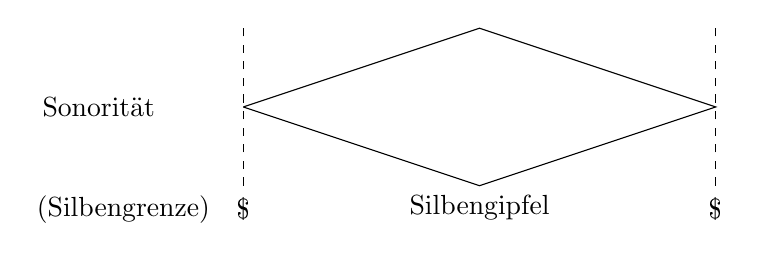
\begin{tikzpicture}
	\draw[dashed] (-3,0)--(-3,2);
	\draw[dashed] (3,0)--(3,2);
	\draw[black] (-3,1)--(0,2)--(3,1)--(0,0)--(-3,1);
	\node at (-3,-0.3){\$};
	\node at (3,-0.3){\$};
	\node[left] at (-3.3,-0.3){(Silbengrenze)};
	\node[left] at (-4,1){Sonorität};
	\node[below] at (0,0){Silbengipfel};
	\end{tikzpicture}
	\caption{\citet[93]{Ramers08a} \citep[nach][]{Lenerz85a}}
\end{figure}
% Vokale sind sonorste Elemente
% m > p
% s > p  (frikativ > plosiv)

\begin{itemize}
	\item Laute können nach der Sonoritätshierarchie auf einer Skala (nach ihrer \textbf{Sonorität}) angeordnet werden.
\end{itemize}

\end{frame}


%%%%%%%%%%%%%%%%%%%%%%%%%%%%%%%%%%
\begin{frame}
\frametitle{Varianten der Sonoritätshierarchie}

Es gibt verschiedene Ausformulierungen der Sonoritätshierachie.


\begin{table}
\centering
\begin{tabular}{l|l|l|l|l} 
	 & einfach 				  	 & Hall 					  & \textbf{Wiese} 				& komplex  \\ 
\hline
\hline 
$[+]$& \multirow{6}{*}{Sonorant} & \multirow{2}{*}{Vokal} 	  & \multirow{2}{*}{Vokal} 		& Vokal  \\ 
	 & 							 & 						 	  &								& Vokal (hoch) \\
\cline{3-5}			
	 &							 & \multirow{3}{*}{Liquide}   &								& Gleitlaut \\
	 &						  	 &	 						  & \textipa{/\textscr /}		& Vibrant \\
\cline{4-5}			
	 &						 	 &							  & \textipa{/l/}				& Lateral \\
\cline{3-5}			
	 &							 & Nasal					  & Nasal						& Nasal \\
\hline			
	 &\multirow{6}{*}{Obstruent} & \multirow{6}{*}{Obstruent} & \multirow{3}{*}{Frikativ}	& $[+$sth$]$ Frikativ \\
	 &						 	 &							  &								& $[+$sth$]$ Affrikat \\		
	 &							 &							  &								& $[+$sth$]$ Plosiv \\
\cline{4-5}			
	 &						  	 &							  & \multirow{3}{*}{Plosiv}		& $[-$sth$]$ Frikativ \\
	 &						 	 &							  &								& $[-$sth$]$ Affrikat \\		
$[-]$&							 &							  &								& $[-$sth$]$ Plosiv \\
		
\end{tabular} 

\end{table}

\end{frame}



%%%%%%%%%%%%%%%%%%%%%%%%%%%%%%%%%%

\begin{frame}
%\frametitle{Sonoritätshierarchie}


\begin{block}{Sonoritätsprinzip (Sonority Sequencing Generalization -- SSG)}
In jeder Silbe gibt es ein Segment, das den \textbf{Silbengipfel} bildet, und dem ein oder mehrere Segmente vorangehen und/oder folgen, deren Sonoritätswerte \textbf{zum Silbengipfel hin zunehmen} und \textbf{danach abnehmen}. (vgl. \citealt[225]{Hall00a}, \citealt[94]{Ramers08a})
\end{block}

\begin{itemize}
	\item Strikt: Monoton steigend oder fallend
	\item Abgeschwächt: auch gleichbleibend \citep[vgl.][]{Hall00a}

\end{itemize}


\begin{figure}
	\centering
	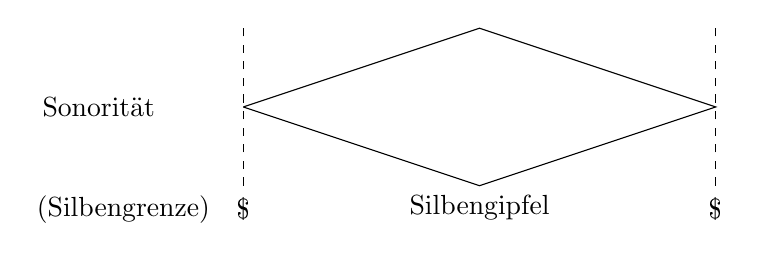
\begin{tikzpicture}
	\draw[dashed] (-3,0)--(-3,2);
	\draw[dashed] (3,0)--(3,2);
	\draw[black] (-3,1)--(0,2)--(3,1)--(0,0)--(-3,1);
	\node at (-3,-0.3){\$};
	\node at (3,-0.3){\$};
	\node[left] at (-3.3,-0.3){(Silbengrenze)};
	\node[left] at (-4,1){Sonorität};
	\node[below] at (0,0){Silbengipfel};
\end{tikzpicture}
\caption{\citet[93]{Ramers08a} \citep[nach][]{Lenerz85a}}
\end{figure}


\end{frame}


%%%%%%%%%%%%%%%%%%%%%%%%%%%%%%%%%%
\begin{frame}
%\frametitle{Sonoritätshierarchie}

\begin{block}{Sonoritätshierarchie (für uns)}
Vokal $>$ \textipa{/\textscr /} $>$ \textipa{/l/} $>$ Nasal $>$ Frikativ $>$ Plosiv \\
$x > y$ $:=$ $x$ ist sonorer als $y$
\end{block}

\begin{figure}
	\centering
	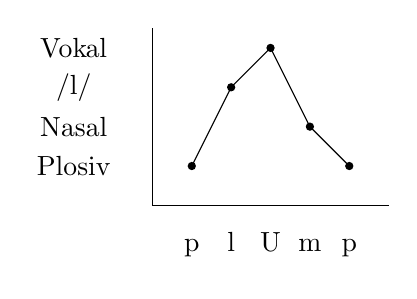
\begin{tikzpicture}[scale=0.5]
	\draw[black] (-1,0) -- (5,0) ; % x axis
	\draw[black] (-1,0) -- (-1,4.5); % y axis
	\node at (-3,1) {Plosiv};
	\node at (-3,2) {Nasal};
	\node at (-3,3) {\textipa{/l/}};
	\node at (-3,4) {Vokal};
	\draw[black] (0,1) -- (1,3) -- (2,4) -- (3,2) -- (4,1);
	\node at (0,-1) {\strut \textipa{p}};
	\node at (1,-1) {\strut \textipa{l}};
	\node at (2,-1) {\strut \textipa{U}};
	\node at (3,-1) {\strut \textipa{m}};
	\node at (4,-1) {\strut \textipa{p}};
	\fill (0,1) circle [radius=3pt];
	\fill (1,3) circle [radius=3pt];
	\fill (2,4) circle [radius=3pt];
	\fill (3,2) circle [radius=3pt];
	\fill (4,1) circle [radius=3pt];
	\end{tikzpicture}
\caption{\citet[225]{Hall00a}}
\end{figure}


%\begin{figure}
%\centering
%\includegraphics[scale=.3]{material/03bSonoritaetBsp}
%\caption{\citet[225]{Hall00a}}
%\end{figure}

\begin{itemize}
	\item Sonoritätshierarchie wird je nach Sprache leicht anders spezifiziert.
\end{itemize}
\end{frame}


%%%%%%%%%%%%%%%%%%%%%%%%%%%%%%%%%%
\begin{frame}
\frametitle{Übung}

\begin{itemize}
	\item Geben Sie die Sonoritätsprofile der folgenden Silben an.
	
	\ea Spatz, Dachs, Clown, Milch
	\z
	
	% bei Spatz geht es von Frikativ s auf Plosiv p runter = Ausnahme
	% bei Dachs geht es auf k runter und dann auf s hoch   = Ausnahme
	% clown k = plosiv, l = /l/ au = Vokal, n = , keine Ausnahme
	
	% Glottal stop gehört zu den Plosiven
	
	\item Erklären Sie die Ungrammatikalität der folgenden Silben:
	
	\begin{exe}
	\ex \label{ex:lbat}
	\begin{xlist}
		\ex [*]{\textipa{[lbat]}}
		\ex [*]{\textipa{[blabl]}}
		\ex [*]{\textipa{[ki:l\textscr]}}
		\ex [*]{\textipa{[ngang]}}
		\ex [*]{\textipa{[krafm]}}
		\ex [*]{\textipa{[elat]}}
		\ex [*]{\textipa{[plaml]}}
		\ex [*]{\textipa{[nfatl]}}
	\end{xlist}
\end{exe}
	
\end{itemize}

\end{frame}


%%%%%%%%%%%%%%%%%%%%%%%%%%%%%%%%%%%
\iftoggle{ue-loesung}{
	%%%%%%%%%%%%%%%%%%%%%%%%%%%%%%%%%%
%% UE 1 - 03b Phonologie
%%%%%%%%%%%%%%%%%%%%%%%%%%%%%%%%%%

\begin{frame}
\frametitle{Übung: Sonoritätsprofile -- Lösung}

\vfill
\hfill
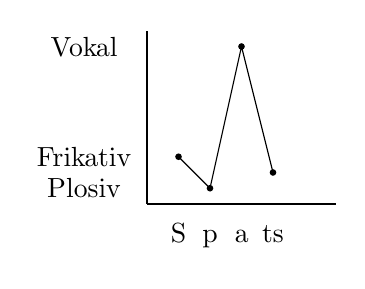
\begin{tikzpicture}[scale=0.4]
\draw[black] (-1,0) -- (5,0) ; % x axis
\draw[black] (-1,0) -- (-1,5.5); % y axis
\node at (-3,0.5) {Plosiv};
\node at (-3,1.5) {Frikativ};
\node at (-3,5) {Vokal};
\draw[black] (0,1.5) -- (1,0.5) -- (2,5) -- (3,1);
\node at (0,-1) {\strut \textipa{S}};
\node at (1,-1) {\strut \textipa{p}};
\node at (2,-1) {\strut \textipa{a}};
\node at (3,-1) {\strut \textipa{\texttoptiebar{ts}}};
\fill (0,1.5) circle [radius=3pt];
\fill (1,0.5) circle [radius=3pt];
\fill (2,5) circle [radius=3pt];
\fill (3,1) circle [radius=3pt];
\end{tikzpicture}
\pause
\hfill
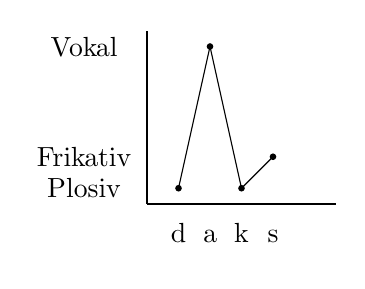
\begin{tikzpicture}[scale=0.4]
\draw[black] (-1,0) -- (5,0) ; % x axis
\draw[black] (-1,0) -- (-1,5.5); % y axis
\node at (-3,0.5) {Plosiv};
\node at (-3,1.5) {Frikativ};
\node at (-3,5) {Vokal};
\draw[black] (0,0.5) -- (1,5) -- (2,0.5) -- (3,1.5);
\node at (0,-1) {\strut \textipa{d}};
\node at (1,-1) {\strut \textipa{a}};
\node at (2,-1) {\strut \textipa{k}};
\node at (3,-1) {\strut \textipa{s}};
\fill (0,0.5) circle [radius=3pt];
\fill (1,5) circle [radius=3pt];
\fill (2,0.5) circle [radius=3pt];
\fill (3,1.5) circle [radius=3pt];
\end{tikzpicture}
\hfill\mbox{}
\vfill
\pause
\hfill
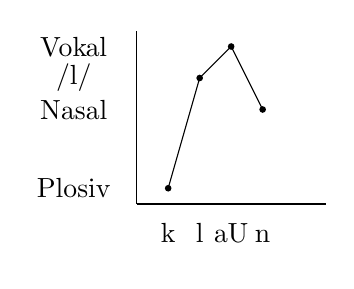
\begin{tikzpicture}[scale=0.4]
\draw[black] (-1,0) -- (5,0) ; % x axis
\draw[black] (-1,0) -- (-1,5.5); % y axis
\node at (-3,0.5) {Plosiv};
\node at (-3,3) {Nasal};
\node at (-3,4) {\textipa{/l/}};
\node at (-3,5) {Vokal};
\draw[black] (0,0.5) -- (1,4) -- (2,5) -- (3,3);
\node at (0,-1) {\strut \textipa{k}};
\node at (1,-1) {\strut \textipa{l}};
\node at (2,-1) {\strut \textipa{\texttoptiebar{aU}}};
\node at (3,-1) {\strut \textipa{n}};
\fill (0,0.5) circle [radius=3pt];
\fill (1,4) circle [radius=3pt];
\fill (2,5) circle [radius=3pt];
\fill (3,3) circle [radius=3pt];
\end{tikzpicture}
\hfill
\pause
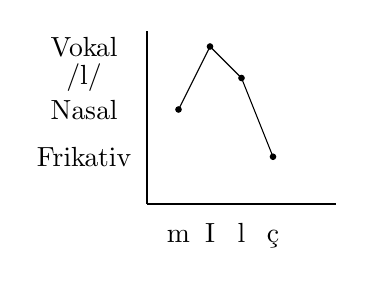
\begin{tikzpicture}[scale=0.4]
\draw[black] (-1,0) -- (5,0) ; % x axis
\draw[black] (-1,0) -- (-1,5.5); % y axis
\node at (-3,1.5) {Frikativ};
\node at (-3,3) {Nasal};
\node at (-3,4) {\textipa{/l/}};
\node at (-3,5) {Vokal};
\draw[black] (0,3) -- (1,5) -- (2,4) -- (3,1.5);
\node at (0,-1) {\strut \textipa{m}};
\node at (1,-1) {\strut \textipa{I}};
\node at (2,-1) {\strut \textipa{l}};
\node at (3,-1) {\strut \textipa{\c{c}}};
\fill (0,3) circle [radius=3pt];
\fill (1,5) circle [radius=3pt];
\fill (2,4) circle [radius=3pt];
\fill (3,1.5) circle [radius=3pt];
\end{tikzpicture}
\hfill\mbox{}
\vfill
\end{frame}


%%%%%%%%%%%%%%%%%%%%%%%%%%%%%%%%%%
\begin{frame}
\frametitle{Übung -- Lösung}

\begin{itemize}
\item Erklären Sie die Ungrammatikalität der folgenden Silben:

\begin{exe}
	\exr{ex:lbat}
	\settowidth\jamwidth{XXXXXXXXXXXXXXXXXXXXXXXXXXXXXXXXXX}
	\begin{xlist}
		\ex[*]{ \textipa{[lbat]}\loesung{2}{\textipa{[l]} vor \textipa{[b]} im Onset} }
		\ex[*]{ \textipa{[blabl]}\loesung{3}{\textipa{[b]} vor \textipa{[l]} in der Koda $+$ Auslautverhärtung} }
		\ex[*]{ \textipa{[m{\textscr}apt]}\loesung{4}{\textipa{[m]} vor \textipa{[\textscr ]} im Onset} }
		\ex[*]{ \textipa{[ki:l\textscr]}\loesung{5}{\textipa{[l]} vor \textipa{[\textscr ]} in der Koda} }
		\ex[*]{ \textipa{[ngang]}\loesung{6}{\textipa{[n]} vor \textipa{[g]} im Onset $+$ reg. velare Nasalassimiliation } \loesung{6}{$+$ g-Tilgung}}
		\ex[*]{ \textipa{[krafm]}\loesung{7}{\textipa{[f]} vor \textipa{[m]} in der Koda} }
		\ex[*]{ \textipa{[elat]}\loesung{8}{2 Silben (2 Nuklei) $+$ Knacklauteinsetzung} }
		\ex[*]{ \textipa{[plaml]}\loesung{9}{\textipa{[m]} vor \textipa{[l]} in der Koda} }
		\ex[*]{ \textipa{[nfatl]}\loesung{10}{\textipa{[n]} vor \textipa{[f]} im Onset $+$ \textipa{[t]} vor \textipa{[l]} in der Koda} }
	\end{xlist}
\end{exe}

\end{itemize}

\end{frame}


}
%%%%%%%%%%%%%%%%%%%%%%%%%%%%%%%%%%

\subsubsection{Weitere phonotaktische Beschränkungen}

%%%%%%%%%%%%%%%%%%%%%%%%%%%%%%%%%%

\begin{frame}
\frametitle{Weitere phonotaktische Beschränkungen}

\begin{columns}
	
	\column{.6\textwidth}	
\begin{itemize}
	\item Im \textbf{Onset} in deutschen Silben können stehen:
	
	\begin{itemize}
		\item alle Einzelkonsonanten des Deutschen 
		
		(\textbf{außer} \textipa{[N]} und \textipa{[s]} vor Vokal am Wortanfang)

		\item bestimmte zwei- und dreigliedrige Konsonantencluster nach Sonoritätshierarchie
		
		\item bestimmte zweigliedrige Konsonantencluster\\
		 (s. Tabelle: von links nach oben im Onset, in der Koda umgekehrt, \citealp[vgl.][231-235]{Hall00a})
	\end{itemize}

	\ea *\textipa{[fma]} \vs \textipa{[fla]}
	\ex *\textipa{[lpa]} \vs \textipa{[pla]}
	\ex *\textipa{[mSa]} \vs \textipa{[Sma]}
	\ex *\textipa{[m\;Ra]}
	\z
\end{itemize}
	
	\column{.35\textwidth}
\begin{table}
	\centering
	
	\begin{tabular}{c|c|c|c|c}
		& \textipa{m} & \textipa{n} & \textipa{l} & \textipa{\textscr} \\ 
		\hline 
		\textipa{p} &  &  & $+$ & $+$ \\ 
		\hline 
		\textipa{b} &  &  & $+$ & $+$ \\ 
		\hline 
		\textipa{t} &  &  &  & $+$ \\ 
		\hline 
		\textipa{d} &  &  &  & $+$ \\ 
		\hline 
		\textipa{k} &  & $+$ & $+$ & $+$ \\ 
		\hline 
		\textipa{g} &  & $+$ & $+$ & $+$ \\ 
		\hline 
		\textipa{f} &  &  & $+$ & $+$ \\
		\hline 
		\textipa{v} &  &  &  & $+$ \\ 
		\hline 
		\textipa{S} & $+$ & $+$ & $+$ & $+$ \\ 
	\end{tabular} 
	
	\caption{Kombinatorik von Sonoranten mit Obstruenten im Deutschen}
\end{table}

\end{columns}	

\end{frame}	
%%%%%%%%%%%%%%%%%%%%%%%%%%%%%%%%%

\begin{frame}{Weitere phonotaktische Beschränkungen}
	
\begin{itemize}	
	\item Silben können auch \textbf{mit unbetontem Vokal} beginnen (\ras leerer Onset).
	\ea \ab{Eier}: \textipa{[\textprimstress P\t{aɪ}.\alertred{5}]}
	\z
	
	\ea \ab{etwaig}: \textipa{[PEt.\textprimstress va:.\alertred{I}\c{c}]} 
	\z

\pause 
	
	\item Vor betontem Vokal steht immer ein Konsonant (\textbf{Glottisschlag}).
	
	\ea
	\textipa{[ka.\alertred{\textprimstress Po:}.tIS]}
	\z

\end{itemize}

\end{frame}


%%%%%%%%%%%%%%%%%%%%%%%%%%%%%%%%%%
\subsection{Hausaufgabe}
%%%%%%%%%%%%%%%%%%%%%%%%%%%%%%%%%%

\begin{frame}
\frametitle{Hausaufgabe}

\begin{itemize}
	\item[1.]{Geben Sie die standarddeutsche \textbf{phonetische Transkription} für folgende Wörter an:}
	
	\eal \label{ex:03bHA1}
	\ex Spitzenschuhe
	\ex Endausscheidung
	\ex Platzanweiser
	\ex verzweifeln
	\ex abverlangen
	\ex Überarbeitung
	\ex Zugeständnis
	\zl
\end{itemize}

\end{frame}
%%%%%%%%%%%%%%%%%%%%%%%%%%%%%%%%%

\begin{frame}{Hausaufgabe}

\begin{itemize}
\item[2.]{Erläutern Sie anhand der folgenden Beispiele, unter welchen Bedingungen die \textbf{Auslautverhärtung} im Deutschen stattfindet.}

\eal \label{ex:03bHA2}
\ex Wand -- Wände
\ex lesen -- lesbar
\ex sagen -- sagst
\ex Roggen
\exi{}{Für Fortgeschrittene auch noch:}
\ex schnell gesprochenes \textit{hab' ich}
\zl

\end{itemize}

\end{frame}
%%%%%%%%%%%%%%%%%%%%%%%%%%%%%%%%%%

\begin{frame}{Hausaufgabe}

\begin{itemize}
\item[3.]{Geben Sie fünf verschiedene \textbf{phonetische oder phonologische Prozesse} an, die in dem folgenden Satz -- teilweise nur bei schnellerem Sprechen -- beobachtet werden können.} 

\ea \label{ex:03bHA3}
\begin{quote}
Um die fünf Haken in regelmäßigen Abständen an die Wand schrauben zu können, sollten Sie sich Bohrmaschine, Wasserwaage, Zollstock und Dübel bereitgelegt haben und auf keinen Fall die Nerven verlieren, bevor Sie nicht befestigt sind.
\end{quote}
\z

\end{itemize}

\end{frame}
%%%%%%%%%%%%%%%%%%%%%%%%%%%%%%%%%%%

\begin{frame}{Hausaufgabe}

\begin{itemize}	
\item[4.]{Illustrieren Sie den deutschen phonemischen Kontrast der folgenden Phoneme durch \textbf{Minimalpaare}, wobei der Kontrast (wenn möglich) ein Mal initial, ein Mal final vorkommen soll.

Beispiel: \textipa{[p]} -- \textipa{[f]} Paul -- faul (Initialposition), Laub -- Lauf (Finalposition)}

\eal \label{ex:03bHA4}
\ex \textipa{[m]} -- \textipa{[n]}
\ex \textipa{[p]} -- \textipa{[b]}
\ex \textipa{[h]} -- \textipa{[v]}
\ex \textipa{[n]} -- \textipa{[N]}
\ex \textipa{[f]} -- \textipa{[v]}
\zl

\end{itemize}
\end{frame}


%%%%%%%%%%%%%%%%%%%%%%%%%%%%%%%%%%%
\iftoggle{ha-loesung}{
	%%%%%%%%%%%%%%%%%%%%%%%%%%%%%%%%%%
%% HA 1 - 03b Phonologie
%%%%%%%%%%%%%%%%%%%%%%%%%%%%%%%%%%

\begin{frame}
\frametitle{Hausaufgabe -- Lösung}

\begin{itemize}
	\item[1.]{Geben Sie die standarddeutsche \textbf{phonetische Transkription} für folgende Wörter an:}
	
	\begin{exe}
		\exr{ex:03bHA1}
		\begin{xlist}
		\settowidth\jamwidth{XXXXXXXXXXXXXXXXXXXXXXXXXXXXXX}
			\ex Spitzenschuhe \loesung{2}{\textipa{['SpI\textsubdot{\t{ts}}@n.Su:.@]}}
			\ex Endausscheidung \loesung{3}{\textipa{['PEnt.P\texttoptiebar{aU}s.S\texttoptiebar{aI}.dUN]}}
			\ex Platzanweiser \loesung{4}{\textipa{['pla\texttoptiebar{ts}.Pan.v\texttoptiebar{aI}.z5]}}
			\ex verzweifeln \loesung{5}{\textipa{[fE5.'\texttoptiebar{ts}v\texttoptiebar{aI}.f@ln]}}
			\ex abverlangen \loesung{6}{\textipa{['Pap.fE5.la\.N@n]}}
			\ex Überarbeitung \loesung{7}{\textipa{[Py:.b5.'Pa\;R.b\texttoptiebar{aI}.tUN]}}
			\ex Zugeständnis \loesung{8}{\textipa{['\texttoptiebar{ts}u:.g@.StEnt.nIs]}}
		\end{xlist}
	\end{exe}

\end{itemize}

\end{frame}
%%%%%%%%%%%%%%%%%%%%%%%%%%%%%%%%%

\begin{frame}{Hausaufgabe -- Lösung}

\begin{itemize}
	\item[2.]{Erläutern Sie anhand der folgenden Beispiele, unter welchen Bedingungen die \textbf{Auslautverhärtung} im Deutschen stattfindet.}

	\begin{exe}
		\exr{ex:03bHA2}
		\begin{xlist}
		\settowidth\jamwidth{XXXXXXXXXXXXXXXXXXXXXXXXXXXXXXX}
			\ex Wand -- Wände \loesung{2}{sth. Plosive am Wortende}
			\ex lesen -- lesbar \loesung{3}{generell am Silbenende}
			\ex sagen -- sagst \loesung{4}{betrifft \emph{alle} sth. Plosive in der Koda}
			\ex Roggen \loesung{5}{jedoch keine Silbengelenke}
		\end{xlist}
	\end{exe}

\end{itemize}

\end{frame}


%%%%%%%%%%%%%%%%%%%%%%%%%%%%%%%%%%
\begin{frame}{Hausaufgabe -- Lösung}

\begin{itemize}
\item[3.]{Geben Sie fünf verschiedene \textbf{phonetische oder phonologische Prozesse} an, die in dem folgenden Satz -- teilweise nur bei schnellerem Sprechen -- beobachtet werden können.} 

\begin{exe}
	\exr{ex:03bHA3}
	\begin{quote}
	Um die fünf Haken in regelmäßigen Abständen an die Wand schrauben zu können, sollten Sie sich Bohrmaschine, Wasserwaage, Zollstock und Dübel bereitgelegt haben und auf keinen Fall die Nerven verlieren, bevor Sie nicht befestigt sind.
	\end{quote}
\end{exe}


\begin{description}
	\item[\alertred{\textbf{Beispiele:}}] ~

\alertred{
	regressive Nasalassimilation in \emph{fünf}: \textipa{[fY\textbf{m}f]}\\
	progressive Nasalassimilation nach Schwa-Elision (feeding) in \emph{Haken}: \textipa{[hak\textbf{N}]}\\
	Auslautverhärtung in \emph{Wand}: \textipa{[van\textbf{t}]}\\
	progressive Nasalassimilation nach Schwa-Elision (feeding) in \emph{schrauben}: \textipa{[S\;R\t{aU}b\textbf{m}]}\\
	g-Spirantisierung in \emph{befestigt}: \textipa{[b@fEstI\textbf{\c{c}}t]}\\
	r-Vokalisierung in \emph{Bohrmaschine}: \textipa{[bo\textbf{5}maSi:n@]}
}						
		\end{description}

\end{itemize}

\end{frame}


%%%%%%%%%%%%%%%%%%%%%%%%%%%%%%%%%%%
\begin{frame}{Hausaufgabe -- Lösung}

\begin{itemize}	
\item[4.]{Illustrieren Sie den deutschen phonemischen Kontrast der folgenden Phoneme durch \textbf{Minimalpaare}, wobei der Kontrast (wenn möglich) ein Mal initial,\\ ein Mal final vorkommen soll.

Beispiel: \textipa{[p]} -- \textipa{[f]} Paul -- faul (Initialposition), Laub -- Lauf (Finalposition)}

\begin{exe}
	\exr{ex:03bHA4}
	\settowidth\jamwidth{XXXXXXXXXXXXXXXXXXXXXXXXXXXXXXXXXXXX}
	\begin{xlist}
		\ex \textipa{[m]} -- \textipa{[n]} \loesung{2}{muss -- Nuss, beim -- Bein}
		\ex \textipa{[p]} -- \textipa{[b]} \loesung{3}{Pass -- Bass}
			\loesung{3}{(wegen Auslautverhärtung kein finaler Kontrast möglich)}
		\ex \textipa{[h]} -- \textipa{[v]} \loesung{4}{heiß -- weiß (\textipa{[h]} kommt nicht final vor)}
		\ex \textipa{[n]} -- \textipa{[N]} \loesung{5}{Sinn -- sing (\textipa{[N]} kommt nicht initial vor)}
		\ex \textipa{[f]} -- \textipa{[v]} \loesung{6}{Fass -- was}
			\loesung{6}{(wegen Auslautverhärtung kein finaler Kontrast möglich)}
	\end{xlist}
\end{exe}
		
\end{itemize}

\end{frame}

}
%%%%%%%%%%%%%%%%%%%%%%%%%%%%%




%@EE: Checken: Keine Abbildungen und elektronischen Quellen?


%
%%%%%%%%%%%%%%%%%%%%%%%%%%%%%%%%%%%%%%%%%%%%%%%%%
%% Compile the master file!
%% 		Include: Antonio Machicao y Priemer
%% 		Course: GK Linguistik
%%%%%%%%%%%%%%%%%%%%%%%%%%%%%%%%%%%%%%%%%%%%%%%%


%%%%%%%%%%%%%%%%%%%%%%%%%%%%%%%%%%%%%%%%%%%%%%%%%%%%
%%%             Metadata                         
%%%%%%%%%%%%%%%%%%%%%%%%%%%%%%%%%%%%%%%%%%%%%%%%%%%% 

\title{Grundkurs Linguistik}

\subtitle{Graphematik}

\author[A. Machicao y Priemer]{
	{\small Antonio Machicao y Priemer}
	\\
	{\footnotesize \url{http://www.linguistik.hu-berlin.de/staff/amyp}}
	%	\\
	%	{\small\href{mailto:mapriema@hu-berlin.de}{mapriema@hu-berlin.de}}
}

\institute{Institut für deutsche Sprache und Linguistik}

% bitte lassen, sonst kann man nicht sehen, von wann die PDF-Datei ist.
%\date{ }

%\publishers{\textbf{6. linguistischer Methodenworkshop \\ Humboldt-Universität zu Berlin}}

%\hyphenation{nobreak}


%%%%%%%%%%%%%%%%%%%%%%%%%%%%%%%%%%%%%%%%%%%%%%%%%%%%
%%%             Preamble's End                  
%%%%%%%%%%%%%%%%%%%%%%%%%%%%%%%%%%%%%%%%%%%%%%%%%%%%   


%%%%%%%%%%%%%%%%%%%%%%%%%   
\huberlintitlepage[22pt]
\iftoggle{toc}{
	\frame{
		\begin{multicols}{2}
			\frametitle{Inhaltsverzeichnis}
			\tableofcontents
			%[pausesections]
		\end{multicols}
	}
}

%%%%%%%%%%%%%%%%%%%%%%%%%%%%%%%%%%
%%%%%%%%%%%%%%%%%%%%%%%%%%%%%%%%%%
%%%%%LITERATURE:

%% Allgemein
\nocite{Glueck&Roedel16a}
\nocite{Schierholz&Co18}
\nocite{Luedeling2009a}
\nocite{Meibauer&Co07a} 
\nocite{Repp&Co15a} 

%%% Sprache & Sprachwissenschaft
%\nocite{Fries16c} %Adäquatheit
%\nocite{Fries16a} %Grammatikalität
%\nocite{Fries&MyP16c} %GG
%\nocite{Fries&MyP16b} %Akzeptabilität
%\nocite{Fries&MyP16d} %Kompetenz vs. Performanz

%%% Phonetik & Phonologie
%\nocite{Altmann&Co07a}
%\nocite{DudenAussprache00a}
%\nocite{Hall00a} 
%\nocite{Kohler99a}
%\nocite{Krech&Co09a}
%\nocite{Pompino95a}
%\nocite{Ramers08a}
%\nocite{Ramers&Vater92a}
%\nocite{Rues&Co07a}
%\nocite{WieseR96a}
%\nocite{WieseR11a}

%% Graphematik
\nocite{Altmann&Co07a}
\nocite{Duerscheid04a}
\nocite{Eisenberg00a}
\nocite{Fuhrhop08a}
\nocite{Fuhrhop09a}
\nocite{Fuhrhop&Co13a}


%%%%%%%%%%%%%%%%%%%%%%%%%%%%%%%%%%
%%%%%%%%%%%%%%%%%%%%%%%%%%%%%%%%%%
\section{Graphematik}
%%%%%%%%%%%%%%%%%%%%%%%%%%%%%%%%%%


%%%%%%%%%%%%%%%%%%%%%%%%%%%%%%%%%%
\begin{frame}
	\frametitle{Begleitlektüre}
	
	\begin{itemize}
		\item \textbf{obligatorisch:}
		\begin{itemize}
			\item[] AM S.~30--34
			\item[] \citet{Eisenberg04}: Kapitel 8 (S.~301--327)
		\end{itemize}
	\end{itemize}

\end{frame}


%%%%%%%%%%%%%%%%%%%%%%%%%%%%%%%%%%
%%%%%%%%%%%%%%%%%%%%%%%%%%%%%%%%%%
\subsection{Einführung}

%% MyP: Contents
\iftoggle{sectoc}{
	\frame{
		%\begin{multicols}{2}
		\frametitle{~}
		\tableofcontents[currentsubsection, subsubsectionstyle=hide]
		%\end{multicols}
	}
}

%% StM: Contents
\iftoggle{gliederung}{
	
	\outline{
		\begin{itemize}
			
			\item \blaubf{Einführung}
			\item Graph, Graphem, Allograph
			\item Graphematik \vs Orthographie
			\item Schrifttypen \& -systeme
			%%Phonographische Schrifttypen
			%%Logographische Schrifttypen
			%%Fazit: Schrifttypen & -systeme
			%%Tiefe vs. flache Systeme
			\item Graphematische Prinzipien
			%%Phonographisches Prinzip
			%%Silbisches Prinzip
			%%Morphologisches Prinzip
			%%Differenzierung homophoner Formen
			%%Etymologische Schreibung
			%%Ästhetische Schreibung
			%%Syntaktische Schreibung
			\item Hausaufgabe
			
		\end{itemize}
	}
}


%%%%%%%%%%%%%%%%%%%%%%%%%%%%%%%%%%
\begin{frame}
\frametitle{Einführung}

\begin{block}{Graphematik (auch Graphemik)}
	 \textbf{linguistische Teildisziplin}, die sich mit der \textbf{schriftlichen Seite} der Sprache beschäftigt
\end{block}

\pause 

\begin{itemize}

	\item \textbf{Schriftlichkeit} \vs \textbf{Mündlichkeit}
	
	\begin{itemize}
		\item materielle Unterschiede
		\item Unterschied im Gebrauch bzgl.\ Zeitpunkt der Produktion und der Rezeption
		
		\begin{itemize}
			\item  \textbf{Produktion:} 
			
			geschriebener Text benötigt Informationen, die sonst von \textbf{Äußerung oder Kontext} in der gesprochenen Kommunikation gegeben wären.
	
			\item \textbf{Rezeption:} 
			
			geschriebener Text ist \textbf{unabhängig von Zeit und Kontext}.
			
			Einheitlichkeitsregeln werden benötigt, um \textbf{unabhängig verständlich} zu bleiben.
		\end{itemize}

	\end{itemize} 

\end{itemize}

\end{frame}


%%%%%%%%%%%%%%%%%%%%%%%%%%%%%%%%%%
\begin{frame}
\frametitle{Einführung}

\begin{itemize}
	\item Sätze wie (\ref{ex-du-bist-schlau}) und (\ref{ex-nein}) können sehr unterschiedlich gelesen werden.

	\ea\label{ex-du-bist-schlau}
	Du bist schlau.

	\ex\label{ex-nein}
	Nein.
	\z
	
\pause		

\item In der Mündlichkeit vorhandene Informationen: situativer Kontext, Satzintonation, Mimik und Gestik

\item Mögliche \textbf{Kodierung} in der Schriftlichkeit:

	\ea
	DU bist aber \gqq{schlau}!

\begin{multicols}{2}
	\ex 
		\ea nein
		\ex NEIN
		\ex nein!
		\ex nein.
		\ex NEIN.
		\ex *nein
		\z
\end{multicols}

	\z

\end{itemize}		

\end{frame}


%%%%%%%%%%%%%%%%%%%%%%%%%%%%%%%%%%
\begin{frame}
\frametitle{Einführung}

\begin{itemize}
	\item Eine Sprache, \emph{aber} verschiedene \textbf{Varietäten} (Dialekte)
	
	\begin{itemize}
		\item (\idR) eine einzige gemeinsame \textbf{Rechtschreibung}

		\item problemlose Kommunikation über eine bestimmte räumliche Distanz	

	\end{itemize}

\pause

	\item \textbf{Schrift}: ca. 5\,000 Jahre vs. \textbf{Sprache}: ca. 150\,000 Jahre

	\item Man \textbf{lernt} zuerst das Sprechen, bevor man überhaupt schreiben kann und man \textbf{verlernt} eher das Schreiben als das Sprechen.
\end{itemize}

\end{frame}


%%%%%%%%%%%%%%%%%%%%%%%%%%%%%%%%%%
\begin{frame}
\frametitle{Einführung}

\begin{itemize}
	 \item Schriftlichkeit \ras \textbf{System} mit Inventar von Minimaleinheiten und (mehr oder weniger) vorhersagbaren Regeln

	 \item Graphematik \vs Orthographie
	 
	 \begin{itemize}
	 	\item terminologisch manchmal gleich behandelt

	 	\item aber mit unterschiedlichen Zielen, die sie mit unterschiedlichen Methoden verfolgen
	 \end{itemize}
\end{itemize}

\end{frame}


%%%%%%%%%%%%%%%%%%%%%%%%%%%%%%%%%%
%%%%%%%%%%%%%%%%%%%%%%%%%%%%%%%%%%
\subsection{Graph, Graphem, Allograph}

%% MyP: Contents
\iftoggle{sectoc}{
	\frame{
		%\begin{multicols}{2}
		\frametitle{~}
		\tableofcontents[currentsubsection, subsubsectionstyle=hide]
		%\end{multicols}
	}
}

%% StM: Contents
\iftoggle{gliederung}{
	
	\outline{
		\begin{itemize}
			
			\item Einführung
			\item \blaubf{Graph, Graphem, Allograph}
			\item Graphematik \vs Orthographie
			\item Schrifttypen \& -systeme
			%%Phonographische Schrifttypen
			%%Logographische Schrifttypen
			%%Fazit: Schrifttypen & -systeme
			%%Tiefe vs. flache Systeme
			\item Graphematische Prinzipien
			%%Phonographisches Prinzip
			%%Silbisches Prinzip
			%%Morphologisches Prinzip
			%%Differenzierung homophoner Formen
			%%Etymologische Schreibung
			%%Ästhetische Schreibung
			%%Syntaktische Schreibung
			\item Hausaufgabe
			
		\end{itemize}
	}
}


%%%%%%%%%%%%%%%%%%%%%%%%%%%%%%%%%%
\begin{frame}
\frametitle{Graph, Graphem, Allograph}

\begin{itemize}
	\item Graphem: \textbf{Minimaleinheit} der Graphematik

	\item Analog zum Phonembegriff in der Phonologie
\end{itemize}

\begin{block}{Graphem}
kleinste bedeutungsunterscheidende Einheit des Schriftsystems
\end{block}

\pause 

\begin{itemize}
	\item Grapheme sollten \textbf{nicht mit Buchstaben verwechselt werden}.

	\ea \emph{Schwan} besteht aus 6 Buchstaben, aber aus 4 Graphemen.
	\z 
	 	
	\item Grapheme sind \textbf{abstrakte} und \textbf{funktionale} Einheiten,\\
	die durch Buchstaben oder Buchstabenverbindungen realisiert werden können.
\end{itemize}

\end{frame}


%%%%%%%%%%%%%%%%%%%%%%%%%%%%%%%%%%
\begin{frame}
\frametitle{Graph, Graphem, Allograph}

\begin{itemize}
	\item Grapheme kann man, wie auch die Phoneme, durch \textbf{Minimalpaare} ermitteln.
	
	\pause
	 
\settowidth\jamwidth{XXXXXXXXXXXXXXXXXXXXXXXXXXXXXXXX} 

	\ea \ab{war\alertred{d}} \vs \ab{war\alertred{t}} 
	\jambox{
		\only<3->{\ras \ab{d} \vs \ab{t}}
	}
	
	\ex \ab{w\alertred{a}rt} \vs \ab{w\alertred{o}rt} 
	\jambox{
		\only<3->{\ras \ab{a} \vs \ab{o} }
	}
	
	\ex \ab{\alertred{w}art} \vs \ab{\alertred{p}art} 
	\jambox{
		\only<3->{\ras \ab{w} \vs \ab{p} }
	}
	
	\ex \ab{pa\alertred{r}t} \vs \ab{pa\alertred{ch}t} 
	\jambox{
		\only<3->{\ras \ab{r} \vs \ab{ch} }
	}
	\z
\end{itemize}

\end{frame}


%%%%%%%%%%%%%%%%%%%%%%%%%%%%%%%%%%
\begin{frame}
\frametitle{Graph, Graphem, Allograph}

	\begin{itemize}
		\item \textbf{Graph}: tatsächliche Realisierung eines Graphems
		\item \textbf{Allographe}: unterschiedliche Graphe, die mögliche Realisierung eines Graphems sind
		\item[]
		\item Ein Graph, ein Allograph und ein Graphem notiert man\\
		mit den spitzen Klammern \ab{}.
	
		\ea Graphem: \ab{a}

		\ex	Allographe von \ab{a}: \ab{\textit{a}} \ab{\textswab{a}} \ab{a} \ab{\textfrak{a}} \ab{{\Large \calligra{a}}\,} \ab{\texttt{a}}
		\z 
		
		\item In einigen älteren Arbeiten unterscheidet man die Notation von Graphemen \ab{a} in einfachen spitzen Klammern von der Notation von Graphen $\langle \langle$a$\rangle \rangle$ in doppelten spitzen Klammern.
	\end{itemize}


\end{frame}


%%%%%%%%%%%%%%%%%%%%%%%%%%%%%%%%%%
%%%%%%%%%%%%%%%%%%%%%%%%%%%%%%%%%%
\subsection{Graphematik \vs Orthographie}

%% MyP: Contents
\iftoggle{sectoc}{
	\frame{
		%\begin{multicols}{2}
		\frametitle{~}
		\tableofcontents[currentsubsection, subsubsectionstyle=hide]
		%\end{multicols}
	}
}

%% StM: Contents
\iftoggle{gliederung}{
	
	\outline{
		\begin{itemize}
			
			\item Einführung
			\item Graph, Graphem, Allograph
			\item \blaubf{Graphematik \vs Orthographie}
			\item Schrifttypen \& -systeme
			%%Phonographische Schrifttypen
			%%Logographische Schrifttypen
			%%Fazit: Schrifttypen & -systeme
			%%Tiefe vs. flache Systeme
			\item Graphematische Prinzipien
			%%Phonographisches Prinzip
			%%Silbisches Prinzip
			%%Morphologisches Prinzip
			%%Differenzierung homophoner Formen
			%%Etymologische Schreibung
			%%Ästhetische Schreibung
			%%Syntaktische Schreibung
			\item Hausaufgabe
			
		\end{itemize}
	}
}


%%%%%%%%%%%%%%%%%%%%%%%%%%%%%%%%%%
\begin{frame}
\frametitle{Graphematik \vs Orthographie}

	\begin{itemize}
		\item Die Graphematik ist ein \textbf{Teilbereich der Linguistik}, der sich mit dem (\textbf{unabhängigen} und \textbf{natürlichen}) \textbf{Schriftsystem} befasst.
		
		\begin{itemize}
			\item Hauptaufgabe: \textbf{Erklären}, warum Wörter und Sätze (und darüber hinaus auch Texte) so geschrieben werden
			\item Notwendig: \textbf{Regelmäßigkeiten} und Prinzipien, die dem normalen Schreiben zugrunde liegen
			\item Empirische Basis: Schreibusus
		\end{itemize}
			
		\item Graphematisches System \ras \textbf{natürliches System} (wie das phonologische oder syntaktische System)
		\item ABER:
		
		\begin{itemize}
			\item Erlernen der Schriftsprache \ras \textbf{explizit} und angelehnt an Norm
			\item Erlernen der mündlichen (Erst-)Sprache \ras \textbf{natürlich}	
		\end{itemize}
	\end{itemize}
\end{frame}


%%%%%%%%%%%%%%%%%%%%%%%%%%%%%%%%%%
\begin{frame}
\frametitle{Graphematik \vs Orthographie}

\begin{block}{Graphematik}
	Wissenschaft vom \textbf{Schriftsystem einer Sprache}, die die Regularitäten des
        Schriftsystems auf \textbf{segmentaler} und \textbf{suprasegmentaler} Ebene
        \textbf{beschreibt}.\\
        Diese Regularitäten finden ihre empirische Basis im \textbf{Schreibusus}, \dash darin, wie tatsächlich geschrieben wird \citep[vgl.][140]{Duerscheid04a}.
\end{block}

\end{frame}


%%%%%%%%%%%%%%%%%%%%%%%%%%%%%%%%%%
\begin{frame}
\frametitle{Graphematik \vs Orthographie}

\begin{itemize}
	\item Die Orthographie (Rechtschreibung) ist dagegen eine \textbf{\gqq{willkürliche} Festlegung}. Sie legt fest, was \textbf{\gqq{richtig}} oder \textbf{\gqq{falsch}} (nach einer bestimmten Norm) ist.
	
	\begin{itemize}
		\item Ergebnis der Rechtschreibung:\\
                      \textbf{explizit geregeltes} und \textbf{per Konventionen akzeptiertes} System
		
		\item Die normative Instanz (Orthographie) resultiert häufig aus \textbf{(sprach-)politischen} Entscheidungen.
		
		\item Das aus der Graphematik explizit gemachte Wissen spielt eine bedeutende Rolle für die Entwicklung der Orthographie.

\pause
		
		\item Graphematik: \textbf{Beschreibung} des Schriftsystems
		
		\item Orthographie: \textbf{Normierung} des Schriftsystems
	\end{itemize}
\end{itemize}

\end{frame}


%%%%%%%%%%%%%%%%%%%%%%%%%%%%%%%%%%
\begin{frame}{Graphematik \vs Orthographie}

\begin{block}{Orthographie}
	Disziplin, die das \textbf{Regelsystem}, das dem Schreiber als \textbf{externe Normen} vorgegeben wird, entwickelt. Die normativen Festlegungen basieren \idR auf den in der Graphematik gewonnenen Erkenntnissen \citep[vgl.][141]{Duerscheid04a}.
\end{block}

\end{frame}


%%%%%%%%%%%%%%%%%%%%%%%%%%%%%%%%%%
\begin{frame}
\frametitle{Graphematik \vs Orthographie}

%\begin{itemize}
%	\item[]

Wie wird das Wort \textipa{[\textscr a:t]} geschrieben?

        \pause
	\begin{table}
		\centering
		%\scalebox{0.9}{
		\begin{tabular}{l | c | l}
			\ab{R\alertred{ah}t}, \ab{R\alertred{ah}d} & ah & vgl. \ab{Kahn}\\ 
			\hline
			\ab{R\alertred{aa}d}, \ab{R\alertred{aa}t} & aa & vgl. \ab{Aal}\\ 
			\hline
			\ab{R\alertred{ar}d}, \ab{R\alertred{ar}t} & ar & vgl. \ab{Bart} als \textipa{[ba:t]}\\ 
			\hline
			\ab{R\alertred{ahr}t} & ahr	& vgl. \ab{Fahrt} als \textipa{[fa:t]}\\
			\hline
			\ab{Ra\alertred{d}} & d & vgl. \ab{Bad}\\ 
			\hline
			\ab{Ra\alertred{t}} & t & vgl. \ab{Tat}\\ 
		\end{tabular} 
		%}
	\end{table}

%\end{itemize}
\end{frame}



%%%%%%%%%%%%%%%%%%%%%%%%%%%%%%%%%%
\begin{frame}
\frametitle{Graphematik \vs Orthographie}

\begin{itemize}
	\item \textbf{Graphematisch} sind unterschiedliche Schreibungen möglich.

\pause 
	
	\item \textbf{Orthographisch} gibt es \textbf{nur zwei richtige} Schreibungen: \\
	\ab{Rad} oder \ab{Rat}
	\item[]
	\item Gleiche Lautung, aber verschiedene \gqq{Wörter}
	
	\begin{itemize}
		\item \textbf{Morphemkonstanz} (\su): \ab{Rad} wird mit \ab{d} geschrieben, um die \textbf{morphologische Verwandtschaft} zu anderen Wortformen im Paradigma anzuzeigen.
		
		\ea \ab{Räder}, \ab{Rädern}, \ab{radeln}
		\z 

		\item \textbf{Homonymiedifferenzierung} (\su): Zwei Wörter mit der \textbf{gleichen Lautung, aber verschiedenen Bedeutungen,} sollten möglichst verschieden geschrieben werden.
		
		\begin{itemize}
			\item Unterschiedliche Bedeutungen können anhand der Schrift, aber nicht der Lautung, differenziert werden!
		\end{itemize}
	\end{itemize}
\end{itemize}

\end{frame}


%%%%%%%%%%%%%%%%%%%%%%%%%%%%%%%%%%
\begin{frame}
\frametitle{Graphematik \vs Orthographie}

\begin{itemize}
	\item Die Orthographie legt \idR eine einzige, \textbf{verbindliche Form} für die Schreibung eines Wortes fest.
	
	\begin{itemize}
		\item Orthographische Normierung: möglichst \textbf{geringe Variabilität} in der Schreibung

\pause

		\item Weniger als 1\% der Wörter variabel
			
		\ea Graphik/Grafik, Cousine/Kusine, Friseur/Frisör, Nougat/Nugat, so dass/sodass, mithilfe/mit Hilfe, Orthographie/Orthografie \dots
		\z

\pause 
			
		\item Abweichungen in der Schreibung können auch auf internen, \textbf{nicht-kodifizierten} Normen beruhen.
			
		\ea die Klassiker Bibliothek, Ulla's Lädchen, Hits für Kid's, BahnCard, StudentInnen, Student\_innen, Student*innen\dots
		\z
	\end{itemize}
\end{itemize}

\end{frame}


%%%%%%%%%%%%%%%%%%%%%%%%%%%%%%%%%%
\begin{frame}
\frametitle{Graphematik \vs Orthographie}

\begin{itemize}
	\item Die Kenntnisse aus der \textbf{Graphematik} werden für die \textbf{Orthographie} übernommen, um die Sprache der Art zu \textbf{normieren}, dass Lesen und Schreiben möglichst \textbf{reibungslos} und \textbf{intuitiv} vonstattengeht.
		
%	\textbf{Gemeinsames Ziel} von Graphematik und Orthographie:\\
%	 Schreiben und Lesen möglichst \textbf{reibungslos} und \textbf{intuitiv} gestalten

\medskip 

	\item Regeln müssen systematisch nachvollziehbar sein:
	
	\ea \ab{fertig} nicht mit \ab{v}, sondern mit \ab{f} 
	
	\ab{fer} in \ab{fertig} hat nicht die gleiche Bedeutung wie \ab{ver} in \ab{verpetzt} oder \ab{verschreiben}
	\z

\medskip
	
	\item Beschäftigung mit dem \textbf{Erstspracherwerb} bei Kindern und mit der \textbf{Fehleranalyse} ist für die Erstellung der Prinzipien von besonderer Bedeutung.
\end{itemize}

\end{frame}


%%%%%%%%%%%%%%%%%%%%%%%%%%%%%%%%%%
%%%%%%%%%%%%%%%%%%%%%%%%%%%%%%%%%%
\subsection{Schrifttypen \& -systeme}

%% MyP: Contents
\iftoggle{sectoc}{
	\frame{
		%\begin{multicols}{2}
		\frametitle{~}
		\tableofcontents[currentsubsection, subsubsectionstyle=hide]
		%\end{multicols}
	}
}

%% StM: Contents
\iftoggle{gliederung}{
	
	\outline{
		\begin{itemize}
			
			\item Einführung
			\item Graph, Graphem, Allograph
			\item Graphematik \vs Orthographie
			\item \blaubf{Schrifttypen \& -systeme}
			%%Phonographische Schrifttypen
			%%Logographische Schrifttypen
			%%Fazit: Schrifttypen & -systeme
			%%Tiefe vs. flache Systeme
			\item Graphematische Prinzipien
			%%Phonographisches Prinzip
			%%Silbisches Prinzip
			%%Morphologisches Prinzip
			%%Differenzierung homophoner Formen
			%%Etymologische Schreibung
			%%Ästhetische Schreibung
			%%Syntaktische Schreibung
			\item Hausaufgabe
			
		\end{itemize}
	}
}


%%%%%%%%%%%%%%%%%%%%%%%%%%%%%%%%%%
\begin{frame}
\frametitle{Schrifttypen \& -systeme}


\begin{block}{Schriftsystem}
	Regularitäten in der schriftlichen Realisierung einer bestimmten Sprache
\end{block}

\ea \textbf{Das deutsche Schriftsystem} verwendet das Zeichen \gqq{ß}.
\z 

\pause 

\begin{itemize}
	\item Verschiedene Arten von Schriftsystemen gehören zu einem Schrifttyp. 
	
	\ea Das deutsche, das französische und das englische Schriftsystem gehören zu den \textbf{phonographischen Schrifttypen} \\
	(graphische Einheiten (Buchstaben) entsprechen lautlichen Einheiten).
	\z 
\end{itemize}

\begin{block}{Schrifttyp}
	Art der \textbf{Beziehung} zwischen \textbf{sprachlichen} und \textbf{graphischen} Einheiten
\end{block}	

\end{frame}


%%%%%%%%%%%%%%%%%%%%%%%%%%%%%%%%%%%
\begin{frame}
\frametitle{Übersicht der Schrifttypen \& -systeme}


\begin{figure}
	\centering
	\scalebox{.85}{
	\begin{forest}
	MyP edges
	[\textbf{\alertred{Schrifttypen}}
		[\textbf{logographischer} \\ Schrifttyp
			[Chinesisch \\ Hieroglyphen, tier=word]
		]
		[\textbf{phonographischer} \\ Schrifttyp
			[\textbf{alphabetischer} \\ Schrifttyp
				[\textbf{Konsonant-Vokal-}\\Schriften
					[Latein \\ Griechisch \\ Russisch, tier=word]
				]
				[\textbf{Konsonanten-}\\schriften
					[Hebräisch \\ Arabisch, tier=word]
				]
			]
			[\textbf{syllabischer} \\ Schrifttyp
				[Japanisch \\ Koreanisch, tier=word, name=anchor] {
					\node [right=of anchor]{\textbf{\alertred{Schriftsysteme}}};
			}
			]
		]
	]
	\end{forest}
}
\end{figure}

\end{frame}


%%%%%%%%%%%%%%%%%%%%%%%%%%%%%%%%%%
%%%%%%%%%%%%%%%%%%%%%%%%%%%%%%%%%%
\subsubsection{Phonographische Schrifttypen}
%\iftoggle{sectoc}{
%	\frame{
%		\begin{multicols}{2}
%			\frametitle{~}
%			\tableofcontents[currentsection]
%		\end{multicols}
%	}
%}
%%%%%%%%%%%%%%%%%%%%%%%%%%%%%%%%%%

\begin{frame}
\frametitle{Phonographische Schrifttypen}



\begin{itemize}
	\item Grundformen (\zB Grapheme) sind primär auf \textbf{bedeutungsunterscheidende} Elemente (\zB Phoneme in (\ref{ex:DtGraf}) oder Silben (s.\ Abb.)) im Sprachsystem bezogen \citep[vgl.][76--77]{Duerscheid04a}.
\end{itemize}
	 
\hfill 	 
\begin{minipage}{.47\textwidth}
	\ea\label{ex:DtGraf} Deutsch:
	\ab{k} für Laut \textipa{[k]}
	\z 
\end{minipage}%\hfill%
%%
%%
\begin{minipage}{.5\textwidth}
\begin{figure}
	\centering
	
	\includegraphics[scale=.2]{material/05Table_hiragana}
	\caption{Hiragana mit lat. Umschrift}
	\label{Hiragana}
\end{figure}
\end{minipage}

\end{frame}


%%%%%%%%%%%%%%%%%%%%%%%%%%%%%%%%%%
\begin{frame}
\frametitle{Phonographische Schrifttypen: Syllabisch}

%\begin{minipage}{.59\textwidth}
\begin{itemize}
	\item Korrespondenz zwischen \textbf{graphischem Zeichen} und \textbf{Silbe}
	\item Japanisch, Koreanisch, \dots
	
	%\ex. Japanisch: [Japanisch Package] für die Silbe \textipa{[ka]} (in der Silbenschrift Hiragana)

\end{itemize}
%\end{minipage}\hfill%
%%
%%
%\begin{minipage}{.4\textwidth}
	\begin{figure}
		\centering
		
		\includegraphics[scale=.25]{material/05Table_hiragana}
		\caption{Hiragana mit lat. Umschrift}
%		\label{Hiragana}
	\end{figure}
%\end{minipage}

\end{frame}


%%%%%%%%%%%%%%%%%%%%%%%%%%%%%%%%%%
\begin{frame}
\frametitle{Phonographische Schrifttypen: Alphabetisch}


\begin{itemize}

	\item Korrespondenz zwischen \textbf{graphischem Zeichen} (Buchstaben) und \textbf{Lauten}
	\item Deutsch, Russisch, Arabisch, \dots
	
	\ea Deutsch: \ab{t} für Laut \textipa{[t]}
	\z 
	
	\pause 
	
	\begin{itemize}
		\item \textbf{Konsonant-Vokal-Schrift:} \\
		enthält Grapheme für Konsonanten und Vokale
		\item Deutsch, Russisch, \dots
		
		\item \textbf{Konsonantenschrift:}\\
		enthält Grapheme (fast) nur für Konsonanten \citep[vgl.][358]{Glueck16b} 
		\item nordwestsemitische Schriftarten, Arabisch, Hebräisch, \dots
	\end{itemize}
	
	\end{itemize}

\end{frame}


%%%%%%%%%%%%%%%%%%%%%%%%%%%%%%%%%%
%%%%%%%%%%%%%%%%%%%%%%%%%%%%%%%%%%
\subsubsection{Logographische Schrifttypen}
%\iftoggle{sectoc}{
%	\frame{
%		\begin{multicols}{2}
%			\frametitle{~}
%			\tableofcontents[currentsection]
%		\end{multicols}
%	}
%}
%%%%%%%%%%%%%%%%%%%%%%%%%%%%%%%%%%

\begin{frame}
\frametitle{Logographische Schrifttypen}

\begin{itemize}
	\item Grundformen sind primär auf \textbf{bedeutungstragende} Elemente (\zB Wörter oder Morpheme) im Sprachsystem bezogen \citep[vgl.][76--77]{Duerscheid04a}. 
	
	\item Chinesisch, Teile der ägyptischen Hieroglyphen
\end{itemize}
		
\begin{minipage}{.28\textwidth}
	\begin{figure}
	\centering
	\includegraphics[scale=.45]{material/Chinesemountain-Lee-Sau-Dan}
	\caption[chinese]{Chinesisches Zeichen für `Berg'}\label{ChinBerg}
	\end{figure}
\end{minipage}\hfill%
%%
\begin{minipage}{.68\textwidth}
	\begin{figure}
	\centering
	\includegraphics[scale=.37]{material/04Hieroglyphenzahlen}
	\caption[Hiero]{Hieroglyphenzahlen}\label{Hieroglyphen}
	\end{figure}
\end{minipage}
		
\end{frame}


%%%%%%%%%%%%%%%%%%%%%%%%%%%%%%%%%%
%%%%%%%%%%%%%%%%%%%%%%%%%%%%%%%%%%
\subsubsection{Fazit: Schrifttypen \& -systeme}
%\iftoggle{sectoc}{
%	\frame{
%		\begin{multicols}{2}
%			\frametitle{~}
%			\tableofcontents[currentsection]
%		\end{multicols}
%	}
%}
%%%%%%%%%%%%%%%%%%%%%%%%%%%%%%%%%%

\begin{frame}
\frametitle{Fazit: Schrifttypen \& -systeme}

\begin{itemize}
	\item Vorteil von \textbf{phonographischen} Schriftsystemen:
	
	\begin{itemize}
		\item große Menge von Wörtern mit \textbf{eher kleinem Inventar von Zeichen} (20--30) darstellbar
	\end{itemize}
	
	\item \textbf{Logographische Schrifttypen} benötigen sehr viele Zeichen.
	
	\begin{itemize}
		\item Das chinesische Schriftsystem besteht aus ungefähr 87\,000 Zeichen,\\
                  von denen zwischen 3\,000 und 5\,000 für den Alltag benötigt werden.
	\end{itemize}
	
\pause 	

	\item Vorteil von \textbf{logographischen} Schriftsystemen:
	\begin{itemize}
		\item Sie können auch von Lesern anderer Dialekte \textbf{relativ leicht dekodiert} werden.
	\end{itemize}	
\end{itemize}
\end{frame}


%%%%%%%%%%%%%%%%%%%%%%%%%%%%%%%%%%%%
%\begin{frame}
%\frametitle{Übersicht der Schrifttypen \& -systeme}
%
%
%\begin{figure}
%\centering
%\scalebox{.85}{
%	\begin{forest}
%		MyP edges
%		[\textbf{\alertred{Schrifttypen}}
%			[\textbf{logographischer} \\ Schrifttyp
%			[Chinesisch \\ Hieroglyphen, tier=word]
%			]
%			[\textbf{phonographischer} \\ Schrifttyp
%				[\textbf{alphabetischer} \\ Schrifttyp
%					[\textbf{Konsonant-Vokal-}\\Schriften
%						[Latein \\ Griechisch \\ Russisch, tier=word]
%					]
%					[\textbf{Konsonanten-}\\schriften
%						[Hebräisch \\ Arabisch, tier=word]
%					]
%				]
%				[\textbf{syllabischer} \\ Schrifttyp
%					[Japanisch \\ Koreanisch, tier=word, name=anchor] {
%					\node [right=of anchor]{\textbf{\alertred{Schriftsysteme}}};
%					}
%				]
%			]
%		]
%	\end{forest}
%}
%\end{figure}
%
%\end{frame}
%
%
%%%%%%%%%%%%%%%%%%%%%%%%%%%%%%%%%%
%%%%%%%%%%%%%%%%%%%%%%%%%%%%%%%%%%
\subsubsection{Tiefe \vs flache Systeme}
%\iftoggle{sectoc}{
%	\frame{
%		\begin{multicols}{2}
%			\frametitle{~}
%			\tableofcontents[currentsection]
%		\end{multicols}
%	}
%}
%%%%%%%%%%%%%%%%%%%%%%%%%%%%%%%%%%

\begin{frame}
\frametitle{Tiefe vs.\ flache Systeme}

\begin{itemize}
	\item trotz phonographischer/""alphabetischer Schriftsysteme \ras\\
              sehr verschiedene Schreibung in den unterschiedlichen Sprachen

	\item unterschiedliche \textbf{graphematische (/orthographische) Prinzipien},\\
          die den unterschiedlichen Schreibungen zugrunde liegen

	\item Selten 1-zu-1-Korrespondenz zwischen Phonemen und Graphemen
	
	\begin{itemize}
		\item \textbf{tiefes System}\\ 
		\vs
		\item \textbf{flaches System}
	\end{itemize}
\end{itemize}
\end{frame}


%%%%%%%%%%%%%%%%%%%%%%%%%%%%%%%%%%
\begin{frame}
\frametitle{Tiefe vs.\ flache Systeme}
\begin{itemize}
	
	\item \textbf{flaches System:}

	\begin{itemize}
		
		\item sehr gute 1-zu-1-Abbildung von Phonemen und Graphemen
		
		\item \textbf{Türkisch}
		
		\begin{itemize}
			
			\item 1928: Ersetzung der arabischen Schrift durch die lateinische Schrift
			
			\item besonders gute Phonem-Graphem-Abbildung
		\end{itemize}
	\end{itemize}

\pause 

	\item \textbf{tiefes System:}

\begin{itemize}

	\item Abbildung von Phonemen auf Graphemen, aber mit Einschränkung

	\item \textbf{Englisch} oder \textbf{Französisch}
	
	\begin{itemize}
		\item nicht häufig \textbf{reformiert} \ras starke Abweichung von Aussprache und Schriftform

		\item Englisch: \textbf{altes} und \textbf{gewachsenes} System mit sehr verschiedenen \textbf{Dialekten} in unterschiedlichen Ländern

		\item schriftliche Verständigung zwischen den Varietäten ist nur gewährleistet,\\
		wenn die Phonem-Graphem-Korrespondenz nicht streng durchgezogen wird.
	\end{itemize}
\end{itemize}
\end{itemize}

\end{frame}


%%%%%%%%%%%%%%%%%%%%%%%%%%%%%%%%%%
\begin{frame}
\frametitle{Tiefe vs.\ flache Systeme}


	\ea Türkisch: \\
	\ab{dükkan} für \textipa{[dYkkan]}
	
	\ex Spanisch: \\
	\ab{negocio} für \textipa{[negoTio]}
	
	\ex Englisch: \\
	\ab{business} für \textipa{[bIzn@z]}
	
	\ex Französisch: \\
	\ab{boutique} für \textipa{[butik]}
	\z 
	
\pause	
	
	\ea English: \ab{gh o ti} für \ab{fish} 

\pause  
	
	(\ab{gh} wie in \ab{enou\alertred{gh}}, \ab{o} wie in \ab{w\alertred{o}men}, \ab{ti} wie in \ab{na\alertred{ti}on}
	\z 

\end{frame}


%%%%%%%%%%%%%%%%%%%%%%%%%%%%%%%%%%
\begin{frame}
\frametitle{Tiefe vs.\ flache Systeme}


\begin{figure}
\centering
	\includegraphics[scale=.3]{material/04GraphEnglischPGK}
	\caption{Englisch und PGK}\label{grammarlycard}
%{https://www.facebook.com/grammarly/photos/a.158139670871698.33824.139729956046003/942699349082389/; Autor: Grammarly; Stand: 05.12.16}
\end{figure}

\end{frame}


%%%%%%%%%%%%%%%%%%%%%%%%%%%%%%%%%%
%%%%%%%%%%%%%%%%%%%%%%%%%%%%%%%%%%
\subsection{Graphematische Prinzipien}

%% MyP: Contents
\iftoggle{sectoc}{
	\frame{
		%\begin{multicols}{2}
		\frametitle{~}
		\tableofcontents[currentsubsection, subsubsectionstyle=hide]
		%\end{multicols}
	}
}

%% StM: Contents
\iftoggle{gliederung}{
	
	\outline{
		\begin{itemize}
			
			\item Einführung
			\item Graph, Graphem, Allograph
			\item Graphematik \vs Orthographie
			\item Schrifttypen \& -systeme
			%%Phonographische Schrifttypen
			%%Logographische Schrifttypen
			%%Fazit: Schrifttypen & -systeme
			%%Tiefe vs. flache Systeme
			\item \blaubf{Graphematische Prinzipien}
			%%Phonographisches Prinzip
			%%Silbisches Prinzip
			%%Morphologisches Prinzip
			%%Differenzierung homophoner Formen
			%%Etymologische Schreibung
			%%Ästhetische Schreibung
			%%Syntaktische Schreibung
			\item Hausaufgabe
			
		\end{itemize}
	}
}


%%%%%%%%%%%%%%%%%%%%%%%%%%%%%%%%%%
\begin{frame}
\frametitle{Graphematische Prinzipien/Tendenzen}

\begin{itemize}
	\item \textbf{Schrifttyp} bedingt das graphematische System.
	\item Daraus ergibt sich die \textbf{Gewichtung} (oder Vorhandensein) weiterer
Prinzipien:

	\begin{itemize}
		\item Deutsch: alphabetischer Schrifttyp \ras Abbildung von Phonemen mit Graphemen

		\item Abbildung von Phonemen auf Grapheme $=$ \\
		\textbf{Phonem-Graphem-Korrespondenz} (PGK)
		
		\item Weitere Prinzipien:
		
		\begin{itemize}
			\item \textbf{Wortebene}:\\
			regelhafte Markierung von Silben, Morphemen und Bedeutungseinheiten, \dots

			\item \textbf{Satzebene}: \\
			regelhafte Groß- und Kleinschreibung, Zusammen- und Getrenntschreibung, \dots
		\end{itemize}
	
	\end{itemize}

\end{itemize}
\end{frame}


%%%%%%%%%%%%%%%%%%%%%%%%%%%%%%%%%%
\begin{frame}
\frametitle{Graphematische Prinzipien/Tendenzen}

\begin{itemize}
	\item Das graphematische System des Deutschen wird von diesen
	\textbf{meist regelhaften Prinzipien bestimmt} und dementsprechend
	(anschließend) auch \textbf{normiert}, sodass es nur eine einzige
	mögliche (normierte) Schreibung für ein Wort gibt.
	
	\begin{itemize}
		\item Erkundung und Erklärung von Regelmäßigkeiten des Systems \\
		\ras \textbf{graphematische Herangehensweise}
		
		\item Anwendung der Regelmäßigkeiten mit einem präskriptiven,
		normativen Charakter \\
		\ras \textbf{orthographische Herangehensweise}
	\end{itemize}
\end{itemize}

\end{frame}


%%%%%%%%%%%%%%%%%%%%%%%%%%%%%%%%%%
\begin{frame}
\frametitle{Graphematische Prinzipien/Tendenzen}

\begin{itemize}
	\item Graphematische/Orthographische \gqq{Prinzipien/Tendenzen}:
	
	\begin{itemize}
		\item Phonographisches Prinzip (nach Phonem-Graphem-Korrespondenzen)

		\item Silbisches Prinzip

		\item Morphologisches Prinzip (auch Prinzip der Morphemkonstanz)

		\item Differenzierung homophoner Formen

		\item Etymologische Schreibung

		\item Ästhetische Schreibung 

		\item Syntaktische Schreibung 
	\end{itemize}

\item  Es handelt sich eher um \textbf{Tendenzen} (weniger um Prinzipien), \\
weil sie nicht immer \textbf{regelhaft} sind.

\end{itemize}


\end{frame}


%%%%%%%%%%%%%%%%%%%%%%%%%%%%%%%%%%
%%%%%%%%%%%%%%%%%%%%%%%%%%%%%%%%%%
\subsubsection{Phonographisches Prinzip}
%\iftoggle{sectoc}{
%	\frame{
%		\begin{multicols}{2}
%			\frametitle{~}
%			\tableofcontents[currentsection]
%		\end{multicols}
%	}
%}
%%%%%%%%%%%%%%%%%%%%%%%%%%%%%%%%%%

\begin{frame}
\frametitle{Phonographisches Prinzip}

\begin{itemize}
	\item Phoneme werden mit Graphemen wiedergegeben.
	\item \textbf{Phonem-Graphem-Korrespondenzen} (auch PGK-Regeln)

\pause	

	\item Abbildung von \textbf{Lauten} (Phonen) in Form von Buchstaben (Phon--Graphem)\\ 
	\vs
	\item Abbildung von \textbf{abstrakten, regulären Lautmengen} in
Form von Buchstaben (Phonem--Graphem)

\end{itemize}

\end{frame}


%%%%%%%%%%%%%%%%%%%%%%%%%%%%%%%%%%
\begin{frame}
\frametitle{Phonographisches Prinzip}

\begin{itemize}
	
	\item \textbf{Pro}: Phon $\leftrightarrow$ Graphem

	\begin{itemize}
		\item sehr genaue Abbildung
		\item einfach für den Leser
	\end{itemize}

\pause 
	
	\item \textbf{Contra}: Phon $\leftrightarrow$ Graphem
	
	\begin{itemize}
		\item größeres Inventar an Buchstaben nötig
		
		\ea Unterschiedliche Buchstaben(-kombinationen) für \ab{ch}\\
		\zB in \ab{i\alertred{ch}} und \ab{Bu\alertred{ch}}
		\z 

\pause 		

		\item Variabilität der Aussprache in einem Dialekt und in unterschiedlichen Dialekten
		
		\ea Unterschiedliche Schreibung von \ab{Sport},\\
		\zB \ab{Spo\alertred{R}t}, \ab{Spo\alertred{r}t}, \ab{Spo\alertred{a}t}, \ab{Spo\alertred{ch}t}
		\z 

\pause 
		
		\item \gqq{Verwandtschaft} zwischen Wortformen nicht mehr erkennbar
		
		\ea Unterschiedliche Schreibung von \ab{r}\\
		\zB in \ab{hö\alertred{a}t} \vs \ab{hö\alertred{r}en}
		\z 
	\end{itemize}
\end{itemize}

\end{frame}


%%%%%%%%%%%%%%%%%%%%%%%%%%%%%%%%%%
\begin{frame}
\frametitle{Phonographisches Prinzip}

\begin{itemize}
	\item \textbf{Pro} Phonem $\leftrightarrow$ Graphem
	
	\begin{itemize}
		\item einheitliche Wiedergabe von komplementärer, freier und regionaler \textbf{Allophonie}

		\item \textbf{Definition von Graphem} als kleinste bedeutungsunterscheidende Einheit eines Schriftsystems (parallel zu Phonem)
	\end{itemize}

\pause 
	
	\item \textbf{Contra} Phonem $\leftrightarrow$ Graphem
	
	\begin{itemize}
		\item etwas komplizierter \textbf{für den Leser}
		
		\ea Wann wird ein \ab{ch} wie in \ab{i\alertred{ch}} oder wie in \ab{Bu\alertred{ch}} ausgesprochen?
		\z 
		
		\item ABER: Dafür \textbf{reduziert} sich der \textbf{Lernaufwand} bzgl.\ der Menge von zu lernenden Buchstaben.	
	\end{itemize}
\end{itemize}

\end{frame}


%%%%%%%%%%%%%%%%%%%%%%%%%%%%%%%%%%
\begin{frame}
\frametitle{PGK: Konsonanten}

\begin{table}
\centering
\scalebox{0.8}{
\begin{tabular}{l l l | l l l}
\textbf{Phonem} & \textbf{einige mögliche} & \textbf{Graphem} & \textbf{Phonem} & \textbf{einige mögliche } & \textbf{Graphem} \\
& \textbf{Allophone} & & & \textbf{Allophone} & \\ 
\textipa{/p/} & \textipa{[p], [p\super h]} & \ab{p} & \textipa{/\c{c}/} & \textipa{[\c{c}], [x]} & \ab{ch} \\
\textipa{/t/} & \textipa{[t], [t\super h]} & \ab{t} & \textipa{/v/} & \textipa{[v]} & \ab{w} \\
\textipa{/k/} & \textipa{[k], [k\super h]} & \ab{k} & \textipa{/j/} & \textipa{[j]} & \ab{j} \\
\textipa{/b/} & \textipa{[b], [p]} & \ab{b} & \textipa{/h/} & \textipa{[h]} & \ab{h} \\
\textipa{/d/} & \textipa{[d], [t]} & \ab{d} & \textipa{/m/} & \textipa{[m]} & \ab{m} \\
\textipa{/g/} & \textipa{[g], [k]} & \ab{g} & \textipa{/n/} & \textipa{[n]} & \ab{n} \\
\textipa{/k/+/v/} & [\textsubplus{k}]\textipa{[v]} & \ab{qu} & \textipa{/l/} & \textipa{[l]} & \ab{l} \\
\textipa{/f/} & \textipa{[f]} & \ab{f} & /\textscr{}/ & [\textscr{}], \textipa{[K], [r], [5]} & \ab{r} \\
\textipa{/s/} & \textipa{[s]} & \ab{ß} & \textipa{/\t{pf}/} & \textipa{[\t{pf}]} & \ab{pf} \\
\textipa{/s/} & \textipa{[s]} & \ab{s} &   &   &   \\
\textipa{/z/} & \textipa{[z], [s]} & \ab{s} & \textipa{/\t{ts}/} & \textipa{[\t{ts}]} & \ab{z} \\
\textipa{/S/} & \textipa{[S]} & \ab{sch} & \textipa{/\t{tS}/} & \textipa{[\t{tS}]} & \ab{tsch} \\
	
\end{tabular} 
}
%\caption{Phonem-Graphem-Korrespondenzen für Konsonanten}
\end{table}

\pause 

\ea \textipa{/s/}, \textipa{[s]}, \ab{\alertred{ß}} (zwischensilbisch nach XX im Nukleus): au\ab{\alertred{ß}}er, Mu\ab{\alertred{ß}}e

\ex \textipa{/s/}, \textipa{[s]}, \ab{\alertred{s}} (im Auslaut): da\ab{\alertred{s}}, e\ab{\alertred{s}}

\ex \textipa{/z/}, \textipa{[z], [s]}, \ab{\alertred{s}}: \ab{\alertred{s}}ieh\ab{\alertred{s}}t  
\z 


\end{frame}


%%%%%%%%%%%%%%%%%%%%%%%%%%%%%%%%%%%
\begin{frame}
\frametitle{PGK: Vokale}


\begin{table}
\centering
%\scalebox{0.8}{
\begin{tabular}{l l | l l}
	\textbf{Vokalphonem} & \textbf{Graphem} & \textbf{Vokalphonem} & \textbf{Graphem} \\
	\textbf{(lang und gespannt)} & & \textbf{(kurz und ungespannt)} & \\
	\textipa{/i:/} & \ab{ie} & \textipa{/I/} & \ab{i} \\
	\textipa{/y:/} & \ab{ü} & \textipa{/Y/} & \ab{ü} \\
	\textipa{/e:/} & \ab{e} & & \\
	\textipa{/E:/} & \ab{ä} & \textipa {/E/} & \ab{e} \\
	& & \textipa{/@/} & \ab{e} \\
	\textipa{/\o:/} & \ab{ö} & 	\textipa{/\oe/} & \ab{ö} \\
	\textipa{/A:/} & \ab{a} & \textipa{/a/} & \ab{a} \\
	\textipa{/o:/} & \ab{o} & \textipa{/O/} & \ab{o} \\ 
	\textipa{/u:/} & \ab{u} & \textipa{/U/} & \ab{u} \\
\end{tabular}
%}
%\caption{Phonem-Graphem-Korrespondenzen für Vokale}
\end{table}

\end{frame}


%%%%%%%%%%%%%%%%%%%%%%%%%%%%%%%%%%
\begin{frame}
\frametitle{PGK: Diphthonge}

\begin{table}
	\centering
%	\scalebox{0.8}{
	\begin{tabular}{l l}
		\textbf{Diphthong} & \textbf{Digraph} \\
		\textipa{/\t{aI}/} & \ab{ei} \\
		\textipa{/\t{aU}/} & \ab{au} \\
		\textipa{/\t{O}I/} & \ab{eu} \\	
	\end{tabular}		
%	}
%\caption{Phonem-Graphem-Korrespondenzen für Diphthonge}
\end{table}

\begin{description}
	\item[Digraph] Graphem aus zwei Buchstaben 
	
	\item[Trigraph] Graphem aus drei Buchstaben
\end{description}

\end{frame}


%%%%%%%%%%%%%%%%%%%%%%%%%%%%%%%%%%
\begin{frame}
\frametitle{Übung}

\begin{itemize}
	\item Geben Sie 10 Wörter an, die phonographisch geschrieben werden.
	\item Wie würden Sie die folgenden Wörter phonographisch schreiben?

	\ea\label{ex:04aphilo}
		\ea Philosophie
		\ex Balkon
		\ex Creme
		\ex Mutter
		\ex Streithahn
		\z
	\z
	
\end{itemize}
	
\end{frame}


%%%%%%%%%%%%%%%%%%%%%%%%%%%%%%%%%
%%%%%%%%%%%%%%%%%%%%%%%%%%%%%%%%%
\iftoggle{ue-loesung}{
	%%%%%%%%%%%%%%%%%%%%%%%%%%%%%%%%%%
%% UE 1 - 04a Graphematik
%%%%%%%%%%%%%%%%%%%%%%%%%%%%%%%%%%

\begin{frame}
\frametitle{Übung -- Lösung}

\begin{itemize}
	\item Geben Sie 10 Wörter an, die phonographisch geschrieben werden.
	
		\begin{description}
			\item[\alertred{\textbf{Beispiele:}}] \alertred{Beurteilung, schön, Gabel, suchen, Macht, Lager, kurz, niesen, Zopf, Gewerkschaft}
		\end{description}
	
	\item Wie würden Sie die folgenden Wörter phonographisch schreiben?
		
	\begin{exe}
		\exr{ex:04aphilo}
	\settowidth\jamwidth{XXXXXXXXXXXXXXXXXXXXXXXXXXXXX}
		\begin{xlist}
			\ex Philosophie \loesung{2}{\ab{filosofie}}
			\ex Handy \loesung{3}{\ab{hendie}}
			\ex Balkon \loesung{4}{\ab{balkong}}
			\ex Creme \loesung{5}{\ab{krem} oder \ab{kreme}}
			\ex Mutter \loesung{6}{\ab{muter}}
			\ex Streithahn \loesung{7}{\ab{schtreithan}}
		\end{xlist}
	\end{exe}
		

\end{itemize}

\end{frame}


}

%%%%%%%%%%%%%%%%%%%%%%%%%%%%%%%%%%
\begin{frame}
\frametitle{Übung}

\begin{itemize}	
	\item Versuchen Sie, graphematische Regularitäten und Prinzipien zu finden, die die Unterscheidung "`lang \vs kurz"' bei Vokalen anzeigen. Gibt es Ausnahmen?
	
	\ea\label{ex:04amutter}
	
	\begin{multicols}{2}
		\ea Mutter
		\ex Mehl
		\ex See
		\ex Nase
		\ex dehnen
		\ex gehen
		\ex Bier
		\ex Moor
		\ex an
		\ex zum
		\ex Mann
		\ex man
		\ex Herbst
		\ex Laub
		\ex sehr
		\ex Bohrer
		\z
	\end{multicols}
	
	\z
	
\end{itemize}

\end{frame}


%%%%%%%%%%%%%%%%%%%%%%%%%%%%%%%%%%
%%%%%%%%%%%%%%%%%%%%%%%%%%%%%%%%%%
\iftoggle{ue-loesung}{
	%%%%%%%%%%%%%%%%%%%%%%%%%%%%%%%%%%
%% UE 2 - 04a Graphematik
%%%%%%%%%%%%%%%%%%%%%%%%%%%%%%%%%%

\begin{frame}
\frametitle{Übung -- Lösung}

\begin{itemize}	
	\item Versuchen Sie, graphematische Regularitäten und Prinzipien zu finden, die die Unterscheidung lang \vs kurz bei Vokalen anzeigen. Gibt es Ausnahmen?\\
	
%	\vspace{-.3cm}
	
	\begin{exe}
		\exr{ex:04amutter}
		\begin{xlist}
			\begin{multicols}{4}
				\ex Mutter
				\ex Mehl
				\ex See
				\ex Nase
				\ex dehnen
				\ex gehen
				\ex Bier
				\ex Moor
				\ex rot
				\ex zum
				\ex Mann
				\ex man
				\ex Herbst
				\ex Laub
				\ex sehr
				\ex Bohrer
			\end{multicols}
		\end{xlist}
	\end{exe}
	
\end{itemize}

%\vspace{-.3cm}


\begin{multicols}{2}
\begin{itemize}
\item[\alertgreen{--}] \alertgreen{Diphthonge: lang (n.)}
\item[\alertgreen{--}] \alertgreen{Doppelvokale: lang (c., h.), Sonderfall bei \ab{i}: \ab{ie} (g.)}
\item[\alertgreen{--}] \alertgreen{vor Dehnungs-h: lang (b., e., o., p.)}
\item[\alertgreen{--}] \alertgreen{vor Doppelkonsonant: kurz (a., k.)}
\item[\alertgreen{--}] \alertgreen{vor Konsonantencluster: kurz (m.)}
\item[\alertgreen{--}] \alertgreen{offene Schreibsilben: lang bei Hauptbetonung (d., f.),
\\sonst kurz (d.)}
\item[\alertgreen{--}] \alertgreen{einfach geschlossene Schreibsilben: uneindeutig bei Hauptbetonung\\(i., j., l.), sonst kurz (a., e., f., p.)}
\end{itemize}
\end{multicols}

\end{frame}


}

%%%%%%%%%%%%%%%%%%%%%%%%%%%%%%%%%%
%%%%%%%%%%%%%%%%%%%%%%%%%%%%%%%%%%
\subsubsection{Silbisches Prinzip}
%\frame{
%\frametitle{~}
%	\tableofcontents[currentsection]
%}


%%%%%%%%%%%%%%%%%%%%%%%%%%%%%%%%%%
\begin{frame}
\frametitle{Silbisches Prinzip}

\begin{itemize}
	\item auch durch die Lautstruktur zu begründen, aber nicht reine Phonem-Graphem-Beziehungen \ras Bezug auf Vokalqualität/-quantität
	
	\item In der Graphematik wird (analog zur Silbe in der Phonologie) eine Silbe angenommen \citep[vgl.][]{Fuhrhop08a}:
	
	\begin{itemize}
		\item[]
		\item \textbf{Anfangsrand}: Konsonant(en),\\
		leerer Anfangsrand: \textbf{nackte} Silbe\\
		besetzter Anfangsrand: \textbf{bedeckte} Silbe
		\item[]
		\item \textbf{Silbenkern}: Vokal oder Diphthong
		\item[]
		\item \textbf{Endrand}: Konsonant(en)\\
		leerer Endrand: \textbf{offene} Silbe\\
		besetzter Endrand: \textbf{geschlossene} Silbe
	\end{itemize}
\end{itemize}

\end{frame}


%%%%%%%%%%%%%%%%%%%%%%%%%%%%%%%%%%
\begin{frame}
\frametitle{Silbisches Prinzip: (Un-)Gespanntheit}

\begin{itemize}
	\item Vokalqualität (\dash Gespanntheit) und -quantität (\dash Länge) wird phonographisch nicht eindeutig abgebildet (s.\ PGK für Vokale), aber es gibt \textbf{Tendenzen auf Silbenebene}.
	\item[]
	\item für \textbf{morphologisch einfache Wörter} 
	
	\begin{itemize}
		\item offene Silbe \ras \textbf{gespannter} Vokal: 
		
		\ea \ab{Kl\alertred{o}}, \ab{s\alertred{o}} (weitere Markierung: \ab{Se\alertred{e}}, \ab{Re\alertred{h}})
		\z
		
		\item geschlossene Silbe mit komplexem Endrand \ras \textbf{ungespannter} Vokal: 
		
		\ea
		\ab{Stru\alertred{mpf}}, \ab{Bi\alertred{ld}}
		\z
		
		\item wenige \textbf{Ausnahmen} \citep[vgl.][15]{Fuhrhop09a}: 
		
		\ea
		\ab{Mo\alertred{nd}}, \ab{Ke\alertred{ks}}, \ab{O\alertred{bst}}
		\z
		
	\end{itemize}
\end{itemize}
\end{frame}


%%%%%%%%%%%%%%%%%%%%%%%%%%%%%%%%%%
\begin{frame}
\frametitle{Silbisches Prinzip: (Un-)Gespanntheit}

\begin{itemize}
	\item für \textbf{morphologisch einfache Wörter}
	
	\begin{itemize}
		\item geschlossene Silbe mit einfachem Endrand \ras \textbf{gespannter} oder \textbf{ungespannter} Vokal möglich:
		
		\ea \ab{B\alertred{ee}t} -- \ab{B\alertred{e}tt}, \ab{B\alertred{a}hn} -- \ab{B\alertred{a}nn}
		\z

\pause 
		
		\item \textbf{zusätzliche Markierungen} möglich, aber nicht immer markiert: 
		
		\ea 
			\ea ungespannt/kurz: \ab{a\alertred{n}}, \ab{bi\alertred{s}}
		
			\ex gespannt/lang: \ab{ro\alertred{t}}, \ab{Hu\alertred{t}}
			\z
		\z 
	\end{itemize}
\end{itemize}

\end{frame}


%%%%%%%%%%%%%%%%%%%%%%%%%%%%%%%%%%
\begin{frame}
\frametitle{Silbisches Prinzip: Markierungen der (Un-)Gespanntheit}

	\begin{itemize} 
		\item Markierung der \textbf{Gespanntheit} durch \textbf{Verdoppelung des Vokals} \ab{aa}, \ab{ee}, \ab{oo} oder \ab{\textbf{ie}} 
		
		\ea \ab{B\alertred{ee}t}, \ab{S\alertred{aa}l}, \ab{B\alertred{oo}t}, \ab{T\alertred{ie}r}, \ab{M\alertred{eh}l}
		\z

		\begin{itemize}
			\item lediglich \ab{ee} findet sich auch in offenen Silben, vermutlich weil \ab{e} sowohl für /\textschwa{}/ als auch für \textipa{/e/} steht.
		
		\ea \ab{S\alertred{ee}}, \ab{Arm\alertred{ee}}, \ab{Klisch\alertred{ee}}, \ab{All\alertred{ee}}%, \ab{\textbf{Orchidee}}
		\z
		\end{itemize}
	
		\item vor \textbf{Sonoranten}: Markierung der \textbf{Gespanntheit} durch ein \ab{\textbf{h}} \textbf{nach dem Vokal} (Dehnungs-h) 
		
		\ea \ab{Me\alertred{h}l}, \ab{Bo\alertred{h}rer}, \ab{Ba\alertred{h}n}
		\z
	\end{itemize}

\end{frame}


%%%%%%%%%%%%%%%%%%%%%%%%%%%%%%%%%%
\begin{frame}
\frametitle{Silbisches Prinzip: Ungespanntheit \& Silbengelenk}

\begin{itemize}
	\item \textbf{Ungespanntheit} wird \ua durch die \textbf{Verdopplung des Folgekonsonanten} (Geminatenschreibung) angezeigt, in zweisilbigen Wörtern sind diese Konsonanten dann \textbf{ambisyllabisch} (\dash Silbengelenk): 


\ea \ab{E\alertred{bb}e}, \ab{A\alertred{ff}e}, \ab{Kla\alertred{dd}e}
\z

	\item Achtung: Im Deutschen markiert die \textbf{Konsonantenverdopplung} primär ein \textbf{Silbengelenk}. Silbenkgelenke kommen \textbf{nach kurzen ungespannten Vokalen} vor.
	
	\item In Fällen wie (\ref{ex:GraphGelenk1}) korreliert die Geminatenschreibung mit dem morphologischen Prinzip, vgl.\ (\ref{ex:GraphGelenk2}).

	\ea 
	\ea\label{ex:GraphGelenk1} \ab{Fa\alertred{ll}}, \ab{Ma\alertred{nn}}
	\ex\label{ex:GraphGelenk2} \ab{Fä\alertred{ll}e}, \ab{Mä\alertred{nn}er}
	\z
	\z 
\end{itemize}
\end{frame}


%%%%%%%%%%%%%%%%%%%%%%%%%%%%%%%%%%
\begin{frame}
\frametitle{Silbisches Prinzip: silbentrennendes \ab{h}}
	
	\begin{itemize}
	\item zwischen zwei \textbf{vokalischen Silbenkernen} zur \textbf{Markierung der Zweisilbigkeit}
	
	
	\eal
	\ex \ab{ge-\alertred{h}en}
	\ex \ab{Ru-\alertred{h}e}
	\ex \ab{Mü-\alertred{h}e}
	\zl

\pause
	
	\item besonders häufig in Verben
	\eal
	\ex \ab{se\alertred{h}en}
	\ex \ab{ste\alertred{h}en}
	\zl
	
\pause
	
	\item nicht nach Diphthongen, außer \ab{ei}
	\eal
	\ex \ab{h\alertblue{au}en}
	\ex \ab{sch\alertblue{au}en}
	\ex \ab{lei\alertred{h}en}
	\ex \ab{verzei\alertred{h}en}
	\ex \ab{schr\alertblue{ei}en}
	\zl

	\end{itemize}

\end{frame}


%%%%%%%%%%%%%%%%%%%%%%%%%%%%%%%%%%
%%%%%%%%%%%%%%%%%%%%%%%%%%%%%%%%%%
\subsubsection{Morphologisches Prinzip}
%\iftoggle{sectoc}{
%	\frame{
%		\begin{multicols}{2}
%			\frametitle{~}
%			\tableofcontents[currentsection]
%		\end{multicols}
%	}
%}
%%%%%%%%%%%%%%%%%%%%%%%%%%%%%%%%%%

\begin{frame}
\frametitle{Morphologisches Prinzip}

\begin{itemize}
	\item auch Prinzip der Morphemkonstanz, Stammschreibungsprinzip, Verwandtschaftsprinzip
	
	\item Wörter oder Wortformen, die in einer \textbf{morphologischen Beziehung} stehen, werden ähnlich oder gleich geschrieben.
	
	\eal
	\ex \ab{\alertred{A}pfel} -- \ab{\alertred{Ä}pfel}, nicht \ab{Epfel}
	\ex \ab{Hun\alertred{d}} -- \ab{Hun\alertred{d}e}, nicht \ab{Hunt}
	\ex \ab{gro\alertred{ß}} -- \ab{grö\alertred{ß}er}, nicht \ab{gros}
	\ex \ab{B\alertred{a}\alertblue{ll}} -- \ab{B\alertred{ä}\alertblue{ll}e}, nicht \ab{Bal} und \ab{Belle}
	\zl

	\item Bei einigen (wenigen) Wörtern sind zwei Schreibungen zugelassen, um die Verwandtschaft zu verschiedenen Derivaten des gleichen Morphems zu kennzeichnen.
	
	\ea 
	\ea \ab{aufw\alertred{ä}ndig} zu \ab{Aufw\alertred{a}nd}
	\ex \ab{aufw\alertred{e}ndig} zu \ab{aufw\alertred{e}nden}
	\z
	\z 
\end{itemize}

\end{frame}


%%%%%%%%%%%%%%%%%%%%%%%%%%%%%%%%%%
%%%%%%%%%%%%%%%%%%%%%%%%%%%%%%%%%%
%\subsubsection{Übung}
%\frame{
%\frametitle{~}
%	\tableofcontents[currentsection]
%}

%%%%%%%%%%%%%%%%%%%%%%%%%%%%%%%%%%
\begin{frame}
\frametitle{Übung}

\begin{itemize}
	\item Warum schreibt man \ab{dehnen} mit \ab{h}, obwohl das erste \ab{e} in einer offenen Silbe steht und daher nach silbischen Prinzipien sowieso lang gesprochen werden müsste?
	\item[]
	\item Warum schreibt man \ab{mann} und \ab{ball}, obwohl nach silbischen Prinzipien die Geminate einen ambisyllabischen Konsonanten anzeigt?
	\item[]
	\item Warum sind die Wörter \ab{(du) ziehst}, \ab{säubern} und \ab{(er) fällt} Beispiele für morphologisches Schreiben?
	\item[]
	\item Wie hätte eine Person, die \ab{Rad} und \ab{König} als Beispiele für das morphologische Prinzip anführt, \gqq{phonographisches Schreiben} verstanden?
\end{itemize}


\end{frame}


%%%%%%%%%%%%%%%%%%%%%%%%%%%%%%%%%%
%%%%%%%%%%%%%%%%%%%%%%%%%%%%%%%%%%
\iftoggle{ue-loesung}{
	%%%%%%%%%%%%%%%%%%%%%%%%%%%%%%%%%%
%% UE 3 - 04a Graphematik
%%%%%%%%%%%%%%%%%%%%%%%%%%%%%%%%%%

\begin{frame}
\frametitle{Übung -- Lösung}

\begin{itemize}
	\item Warum schreibt man \ab{dehnen} mit \ab{h}, obwohl das erste \ab{e} in einer offenen Silbe steht und daher nach silbischen Prinzipien sowieso lang gesprochen werden müsste?
		\item[] \alertred{Morphemkonstanz, da bei Flexionsformen wie \ab{dehnst} geschlossene Silbe}
	\item Warum schreibt man \ab{mann} und \ab{ball}, obwohl nach silbischen Prinzipien die Geminate einen ambisyllabischen Konsonanten anzeigt?
		\item<2->[] \alertred{Morphemkonstanz, da Pluralform Silbengelenk hat}
	\end{itemize}


\end{frame}


%%%%%%%%%%%%%%%%%%%%%%%%%%
\begin{frame}
\frametitle{Übung -- Lösung}

\begin{itemize}
	\item Warum sind die Wörter \ab{(du) ziehst}, \ab{säubern} und \ab{(er) fällt} Beispiele für morphologisches Schreiben?
		\item<2->[] \alertred{\ab{h} im Infinitiv silbentrennend, Singular-Flexionsformen sind jedoch einsilbig;}
		\item<3->[] \alertred{\ab{ä} zeigt die Verwandschaft zu \ab{sauber}: laut PGK schriebe man \textipa{[O\texttoptiebar{}I]} \ab{eu};}
		\item<4->[] \alertred{Konsonantenverdopplung wegen Silbengelenk im Infinitiv, Singular-Flexionsformen sind jedoch einsilbig,\\ \ab{ä} wegen \ab{a} im Infinitiv: \textipa{[E]} wäre nach PGK \ab{e}}
	\item Wie hätte eine Person, die \ab{Rad} und \ab{König} als Beispiele für das morphologische Prinzip anführt, \gqq{phonographisches Schreiben} verstanden?
		\item<5->[] \alertred{Verschriftlichung der \emph{phonetischen} (richtig wäre: \emph{phonologische}) Repräsentation}
\end{itemize}


\end{frame}


}

%%%%%%%%%%%%%%%%%%%%%%%%%%%%%%%%%%
%%%%%%%%%%%%%%%%%%%%%%%%%%%%%%%%%%
\subsubsection{Differenzierung homophoner Formen}
%\frame{
%\frametitle{~}
%	\tableofcontents[currentsection]
%}


%%%%%%%%%%%%%%%%%%%%%%%%%%%%%%%%%%
\begin{frame}
\frametitle{Differenzierung homophoner Formen}

\begin{itemize}
	
	\item auch Homonym(ie)differenzierung, -vermeidung
	
	\item \textbf{Gleichlautende Wörter} mit \textbf{unterschiedlicher Bedeutung} werden orthographisch unterschiedlich repräsentiert.
	
	\ea L\alertred{ei}b -- L\alertred{ai}b; S\alertred{ei}te -- S\alertred{ai}te; L\alertred{ie}d -- (Augen)L\alertred{i}d
	\z
	
	\item Aber:
	
	\ea Kiefer -- Kiefer; Bremse -- Bremse; Ton -- Ton
	\z
	
	\item Möglichkeiten zur Homophonendifferenzierung werden also keineswegs konsequent ausgenutzt.
\end{itemize}

\end{frame}


%%%%%%%%%%%%%%%%%%%%%%%%%%%%%%%%%%
%%%%%%%%%%%%%%%%%%%%%%%%%%%%%%%%%%
\subsubsection{Etymologische Schreibung}
%\iftoggle{sectoc}{
%	\frame{
%		\begin{multicols}{2}
%			\frametitle{~}
%			\tableofcontents[currentsection]
%		\end{multicols}
%	}
%}
%%%%%%%%%%%%%%%%%%%%%%%%%%%%%%%%%%

\begin{frame}
\frametitle{Etymologische Schreibung}

\begin{itemize}
	\item Die Schreibung \gqq{\textbf{alter}} oder \textbf{entlehnter} Wörter bleibt erhalten,\\
	auch wenn sie nicht den aktuellen Schreibprinzipien entspricht.
	
	\eal
		\ex \ab{wa\alertred{nn}} statt \ab{wan} (wegen mhd. \ab{wanne})
		%% Hier ist kein Silbengelenk möglich!
		
		\ex \ab{\alertred{C}rem\alertred{e}} statt \ab{Krem}
		
		\ex \ab{Restaurant} statt \ab{Restorong}
		
		\ex \ab{Ort\alertred{h}ogra\alertred{ph}ie} oder \ab{Ort\alertred{h}ografie} statt \ab{Ortografie}
	\zl

\end{itemize}

\end{frame}


%%%%%%%%%%%%%%%%%%%%%%%%%%%%%%%%%%
%%%%%%%%%%%%%%%%%%%%%%%%%%%%%%%%%%
\subsubsection{Ästhetische Schreibung}
%\iftoggle{sectoc}{
%	\frame{
%		\begin{multicols}{2}
%			\frametitle{~}
%			\tableofcontents[currentsection]
%		\end{multicols}
%	}
%}
%%%%%%%%%%%%%%%%%%%%%%%%%%%%%%%%%%

\begin{frame}
\frametitle{Ästhetische Schreibung}

\begin{itemize}
	\item \textbf{Schreibsilben} sollten nicht zu lang und nicht zu kurz sein.
	
	\eal
	\ex \ab{\alertred{S}piel} statt \ab{Schpiel}
	\ex \ab{Schw\alertred{a}n} statt \ab{Schw\alertred{ah}n}
	\zl

\pause 
	
	\item \textbf{Verbot von Doppelschreibungen} von einigen Vokalgraphemen (\ab{i} und \ab{u} sowie Umlaute) -- teilweise bedingt durch \textbf{Verwechslungsgefahr}
	
	\ea
	\ab{ii} wie \ab{ü}; \ab{uu} wie \ab{w}
	\z
	
\pause 
		
	\item Verbot von \textbf{Doppelschreibung von Mehrgraphemen} wie
	
	\eal
		\ex \ab{ng} in \ab{Bearbeitu\textcolor{red}{ngng}en}
		\ex \ab{ch} in \ab{Bü\textcolor{red}{chch}er} 
		\ex \ab{sch} in \ab{graphi\textcolor{red}{schsch}e}
	\zl
	
\end{itemize}

\end{frame}


%%%%%%%%%%%%%%%%%%%%%%%%%%%%%%%%%%
%%%%%%%%%%%%%%%%%%%%%%%%%%%%%%%%%%
\subsubsection{Syntaktisches Prinzip}
%\iftoggle{sectoc}{
%	\frame{
%		\begin{multicols}{2}
%			\frametitle{~}
%			\tableofcontents[currentsection]
%		\end{multicols}
%	}
%}
%%%%%%%%%%%%%%%%%%%%%%%%%%%%%%%%%%

\begin{frame}
\frametitle{Syntaktisches Prinzip}

\begin{itemize}
	\item \textbf{Großschreibung für Substantive} und Substantivierungen von Adjektiven, Verben, Adverbien, Partikeln, usw. 

	\ea das \alertred{J}a, das \alertred{G}estern, das \alertred{I}ch
	\z 
	
	\item Großschreibung von \textbf{Satzanfängen} und in \textbf{Anreden}
	
	\ea \alertred{S}ie, \alertred{I}hr
	\z 

	
	\item Die Großschreibung von Substantiven gibt es nur in der deutschen und luxemburgischen Schreibung.\\
	Während der Rechtschreibreform hat man diskutiert, diese abzuschaffen.\\
	Was denken Sie: Was spräche dafür, was dagegen?

\pause 
	
	\ea Berliner Berliner berlinern berlinernd berlinisches Berlinisch.
	\z 
\end{itemize}

\end{frame}




%%%%%%%%%%%%%%%%%%%%%%%%%%%%%%%%%%
%%%%%%%%%%%%%%%%%%%%%%%%%%%%%%%%%%
%\subsection{Übungen}
%\iftoggle{sectoc}{
%	\frame{
%		\begin{multicols}{2}
%			\frametitle{~}
%			\tableofcontents[currentsection]
%		\end{multicols}
%	}
%}


%%%%%%%%%%%%%%%%%%%%%%%%%%%%%%%%%%
\begin{frame}
\frametitle{Übung}

\begin{itemize}
	\item Welche graphematischen Prinzipien (abgesehen von der phonographischen Schreibung) erklären die Schreibung der folgenden Wörter?
	
	  \ea\label{ex:04azimmer}
	  \begin{multicols}{3}
          \ea \ab{Zimmer}
          \ex \ab{Waise}
          \ex \ab{Wehen}
          \ex \ab{Ruhm}
          \ex \ab{Spaß}
          \ex \ab{Allee}
%          \ex \ab{Gras}
          \z
        \end{multicols}
      \z

	\item Welche graphematische Funktion erfüllt das \ab{h} in den folgenden Wörtern?
	
	  \ea\label{ex:04anacht}
	  \begin{multicols}{4}
          \ea \ab{Nacht}
          \ex \ab{Hilfe}
          \ex \ab{sehen}
          \ex \ab{Mehl}
          \z
        \end{multicols}
      \z
      
	\item Wie würden die folgenden Wörter in phonographischer Schreibung aussehen? Geben Sie zunächst eine phonologische Transkription an (Notation mit /~/) \\
	und schreiben Sie anschließend phonographisch (Notation in \ab{~~}).
	
	\ea\label{ex:04avasenstück}
	\begin{multicols}{3}
		\ea \ab{Handy}
		\ex \ab{Vasenstück}
		\ex \ab{Wannenbad}
		\z
	\end{multicols}
	\z
	
\end{itemize}

\end{frame}

%%%%%%%%%%%%%%%%%%%%%%%%%%%%%%%%
%%%%%%%%%%%%%%%%%%%%%%%%%%%%%%%%%
\iftoggle{ue-loesung}{
%%%%%%%%%%%%%%%%%%%%%%%%%%%%%%%%%%
%% UE 4 - 04a Graphematik
%%%%%%%%%%%%%%%%%%%%%%%%%%%%%%%%%%

\begin{frame}
\frametitle{Übung -- Lösung}

\begin{itemize}
	\item Welche graphematischen Prinzipien (abgesehen von der phonographischen Schreibung) erklären die Schreibung der folgenden Wörter?
	
\begin{exe}
	\exr{ex:04azimmer}
	\settowidth\jamwidth{XXXXXXXXXXXXXXXXXXXXXXXXXXXXXXXXXXX}
	\begin{xlist}
		\ex \ab{Zi\rotul{mm}er} \loesung{1}{silbisches Prinzip: Silbengelenk}
		\ex \ab{W\rotul<2->{a}ise} \loesung{2}{Differenzierung homophoner Formen: zu \ab{weise}}
		\ex \ab{We\rotul<3->{h}en} \loesung{3}{silbisches Prinzip: silbentrennend}
		\ex \ab{Ru\rotul<4->{h}m} \loesung{4}{silbisches Prinzip: Dehnungs-h}
		\ex \ab{\rotul<5->{S}paß} \loesung{5}{ästhetische Schreibung: kein \ab{schp}}
		\ex \ab{A\rotul<6->{llee}} \loesung{6}{silbisches Prinzip: Silbengelenk \ab{ll}, Gespanntheit \ab{ee}}
		%          \ex \ab{Gras}
	\end{xlist}
\end{exe}
	
	\item Welche graphematische Funktion erfüllt das \ab{h} in den folgenden Wörtern?
	
\begin{exe}
	\exr{ex:04anacht}
	\settowidth\jamwidth{XXXXXXXXXXXXXXXXXXXXXXXXXXXXXXXXXXX}
	\begin{xlist}
		\ex \ab{Nacht} \loesung{7}{Teil von Digraph \ab{ch}}
		\ex \ab{Hilfe} \loesung{8}{Phonem-Graphem-Korrespondenz zu \textipa{[h]}}
		\ex \ab{sehen} \loesung{9}{silbentrennend}
		\ex \ab{Mehl} \loesung{10}{Dehnungs-h}
	\end{xlist}
\end{exe}
	
    \end{itemize}

\end{frame}


%%%%%%%%%%%%%%%%%%%%%%%%%%%%%%%%%%%%%%%
\begin{frame}{Übung -- Lösung}

	\begin{itemize}
	\item Wie würden die folgenden Wörter in phonographischer Schreibung aussehen? Geben Sie zunächst eine phonologische Transkription an (Notation mit / ~ /) und schreiben Sie anschließend phonographisch (Notation in \ab{ ~ }).

\begin{exe}
	\exr{ex:04avasenstück}
	\begin{multicols}{3}
	\begin{xlist}
		\ex \ab{Handy} 
		
		\ex \ab{Vasenstück}
		
		\ex \ab{Wannenbad}
		
%		\exi{} 
		\exi{} \only<2->{\alertred{\textipa{/hEn.di/}}}
		\exi{} \only<4->{\alertred{\textipa{/va:.z@n.StYk/}}}
		\exi{} \only<6->{\alertred{\textipa{/va\.n@n.ba:d/}}}

%		\exi{} 
		\exi{} \only<3->{\alertred{\ab{hendi}}}		
		\exi{} \only<5->{\alertred{\ab{wasenschtük}}}		
		\exi{} \only<7->{\alertred{\ab{wanenbad}}}		
	\end{xlist}
	\end{multicols}
\end{exe}
	
	\end{itemize}

\end{frame}


}

%%%%%%%%%%%%%%%%%%%%%%%%%%%%%%%%%%
%%%%%%%%%%%%%%%%%%%%%%%%%%%%%%%%%%
\subsection{Hausaufgabe}
%
%%% MyP: Contents
%\iftoggle{sectoc}{
%	\frame{
%		%\begin{multicols}{2}
%		\frametitle{~}
%		\tableofcontents[currentsubsection, subsubsectionstyle=hide]
%		%\end{multicols}
%	}
%}
%
%%% StM: Contents
%\iftoggle{gliederung}{
%	
%	\outline{
%		\begin{itemize}
%			
%			\item Einführung
%			\item Graph, Graphem, Allograph
%			\item Graphematik \vs Orthographie
%			\item Schrifttypen \& -systeme
%			%%Phonographische Schrifttypen
%			%%Logographische Schrifttypen
%			%%Fazit: Schrifttypen & -systeme
%			%%Tiefe vs. flache Systeme
%			\item Graphematische Prinzipien
%			%%Phonographisches Prinzip
%			%%Silbisches Prinzip
%			%%Morphologisches Prinzip
%			%%Differenzierung homophoner Formen
%			%%Etymologische Schreibung
%			%%Ästhetische Schreibung
%			%%Syntaktische Schreibung
%			\item \blaubf{Hausaufgabe}
%			
%		\end{itemize}
%	}
%}
%
%
%%%%%%%%%%%%%%%%%%%%%%%%%%%%%%%%%%
%%%%%%%%%%%%%%%%%%%%%%%%%%%%%%%%%%

\begin{frame}%[allowframebreaks]
	\frametitle{Hausaufgabe}
	
\begin{itemize}
	
	\item[1.] Kreuzen Sie die korrekten Aussagen an.
	
	\begin{itemize}
		\item[$\circ$] Die Orthographie ist eine linguistische Teildisziplin, die beschreibt wie man schreibt. Die Graphematik ist dagegen keine Teildisziplin der Linguistik, sondern eine \gqq{willkürliche} (normierende) Festlegung.
		\item[$\circ$] Die Graphematik sollte intuitiv beherrschbar sein und das Lesen und Schreiben vereinfachen.
		\item[$\circ$] Das Wort \ab{kalt} ist eine graphematisch \gqq{nackte} Silbe.
		\item[$\circ$] Es gibt im Deutschen eine eindeutige 1-zu-1-Korrespondenz zwischen Buchstaben und Lauten.
		\item[$\circ$] Das Wort \ab{aufwändig} wird aufgrund des morphologischen Prinzips (auch Prinzip der Schemakonstanz, Stammprinzip oder Verwandtschaftsprinzip) mit \ab{ä} geschrieben (vgl. \ab{Aufwand}).
		
		% mächtig Macht / ständig Stand / fällt fallen
	\end{itemize}
\end{itemize}
\end{frame}


%%%%%%%%%%%%%%%%%%%%%%%%%%%%%%%%%%
\begin{frame}
	\begin{itemize}
		\item[2.] Ordnen Sie die graphematischen Prinzipien links den passenden Beispielen für die entsprechenden Prinzipien rechts zu.
		
		NB: Beachten Sie bitte nicht die Großschreibung.
		
		\vspace{.5cm}
								
		\begin{minipage}{0.45\textwidth}
			\centering
			\begin{tabular}{|l|}
				\hline
				(A) Etymologische Schreibung\\
				\hline
				(B) Homonymievermeidung\\
				\hline
				(C) Morphologisches Prinzip\\
				\hline
				(D) Silbische Prinzip\\
				\hline
				(E) Phonographisches Prinzip\\
				\hline
			\end{tabular}
		\end{minipage}
		\hfill%
		\begin{minipage}{0.45\textwidth}
			\centering
			\begin{tabular}{|p{0.075\textwidth}|l|}
				\hline
				& Bad, Bäder \\
				\hline
				& gehen \\
				\hline
				& Cello, *Tschello \\
				\hline
				& Wahl, Wal\\
				\hline
				& Flasche \\
				\hline
			\end{tabular}
		\end{minipage}

	\end{itemize}
\end{frame}


%%%%%%%%%%%%%%%%%%%%%%%%%%%%%%%%%%
\begin{frame}
	\begin{itemize}
		\item[3.] Betrachten Sie die unten angegebenen Kontexte. Diskutieren Sie kurz anhand dieser Beispiele, ob es sich bei der Groß- und Kleinschreibung des markierten Buchstabens um unterschiedliche Grapheme handeln kann oder nicht.
\eal\label{ex:04aHA3}
			\ex Dieser \underline{W}eg ist sehr steil.
			\ex \underline{W}ege, die ich nicht bewandert habe, gibt es viele.
			\ex Meine Schlüssel sind \underline{w}eg.
			\ex \gqq{\underline{W}eg!}, schrie sie mich an und knallte mir die Tür vor der Nase zu.
			\ex Geh \underline{w}eg!
\zl
	\end{itemize}
\end{frame}


%%%%%%%%%%%%%%%%%%%%%%%%%%%%%%%%%%
\begin{frame}
	\begin{itemize}
		\item[4.] Erläutern Sie stichpunktartig, welche (graphematische) Funktionen der Buchstabe \ab{h} in den folgenden Kontexten annimmt:
	\eal\label{ex:04aHA4}
			\ex Ha\underline{h}n:
			\ex nä\underline{h}en:
			\ex bein\underline{h}alten:
			\ex Gesc\underline{h}ichte:
			\ex Geschic\underline{h}te:
			\ex Dip\underline{h}thong:
			\ex Dipht\underline{h}ong:
	\zl
	\end{itemize}
\end{frame}


%%%%%%%%%%%%%%%%%%%%%%%%%%%%%%%%%%
\begin{frame}
	\begin{itemize}
		\item[5.] Geben Sie die \textbf{phonologische} Transkription, die \textbf{phonetische} Transkription und die \textbf{phonographische} Schreibung (nach der Phonem-Graphem-Korrespondenz) des folgenden Wortes an.
		
		\ea\label{ex:04aHA5} Abstellkammer
		\z
		
	\end{itemize}
\end{frame}


%%%%%%%%%%%%%%%%%%%%%%%%%%%%%%%%%
%%%%%%%%%%%%%%%%%%%%%%%%%%%%%%%%%
\iftoggle{ha-loesung}{
	%%%%%%%%%%%%%%%%%%%%%%%%%%%%%%%%%%
%% HA 1 - 04a Graphematik
%%%%%%%%%%%%%%%%%%%%%%%%%%%%%%%%%%

\begin{frame}%[allowframebreaks]
\frametitle{Hausaufgabe -- Lösung}

\begin{itemize}
	
	\item[1.] Kreuzen Sie die korrekten Aussagen an.
	
	\begin{itemize}
		\item[$\circ$] Die Orthographie ist eine linguistische Teildisziplin, die beschreibt wie man schreibt. Die Graphematik ist dagegen keine Teildisziplin der Linguistik, sondern eine \gqq{willkürliche} (normierende) Festlegung.
		
		\item[\alertgreen{$\checkmark$}] \alertgreen{Die Graphematik sollte intuitiv beherrschbar sein und das Lesen und Schreiben vereinfachen.}
		
		\item[$\circ$] Das Wort \ab{kalt} ist eine graphematisch \gqq{nackte} Silbe.
		
		\item[$\circ$] Es gibt im Deutschen eine eindeutige 1-zu-1-Korrespondenz zwischen Buchstaben und Lauten.
		
		\item[\alertgreen{$\checkmark$}] \alertgreen{Das Wort \ab{mächtig} wird aufgrund des morphologischen Prinzips (auch Prinzip der Schemakonstanz, Stammprinzip oder Verwandtschaftsprinzip) mit \ab{ä} geschrieben (vgl. \ab{Macht}).}
	\end{itemize}
\end{itemize}
\end{frame}


%%%%%%%%%%%%%%%%%%%%%%%%%%%%%%%%%%	
\begin{frame}
	\frametitle{Hausaufgabe -- Lösung}

\begin{itemize}
\item[2.] Ordnen Sie die graphematischen Prinzipien links den passenden Beispielen für die entsprechenden Prinzipien rechts zu.

NB: Beachten Sie bitte nicht die Großschreibung.

\vspace{.5cm}

\begin{minipage}{0.45\textwidth}
	\centering
	\begin{tabular}{|l|}
		\hline
		(A) Etymologische Schreibung\\
		\hline
		(B) Homonymievermeidung\\
		\hline
		(C) Morphologisches Prinzip\\
		\hline
		(D) Silbische Prinzip\\
		\hline
		(E) Phonographisches Prinzip\\
		\hline
	\end{tabular}
\end{minipage}
\hfill%
\begin{minipage}{0.45\textwidth}
	\centering
	\begin{tabular}{|p{0.075\textwidth}|l|}
		\hline
		\only<2->{\alertgreen{C}} & Bad, Bäder \\
		\hline
		\only<3->{\alertgreen{D}} & gehen \\
		\hline
		\only<4->{\alertgreen{A}} & Cello, *Tschello \\
		\hline
		\only<5->{\alertgreen{B}} & Wahl, Wal\\
		\hline
		\only<6->{\alertgreen{E}} & Flasche \\
		\hline
	\end{tabular}
\end{minipage}

\end{itemize}
\end{frame}


%%%%%%%%%%%%%%%%%%%%%%%%%%%%%%%%%%	
\begin{frame}%[allowframebreaks]
	\frametitle{Hausaufgabe -- Lösung}
	
\begin{itemize}
\item[3.] Betrachten Sie die unten angegebenen Kontexte. Diskutieren Sie kurz anhand dieser Beispiele, ob es sich bei der Groß- und Kleinschreibung des markierten Buchstabens um unterschiedliche Grapheme handeln kann oder nicht.

\begin{exe}
	\exr{ex:04aHA3}
	\begin{xlist}
	\ex Dieser \underline{W}eg ist sehr steil.
	\ex \underline{W}ege, die ich nicht bewandert habe, gibt es viele.
	\ex Meine Schlüssel sind \underline{w}eg.
	\ex \gqq{\underline{W}eg!}, schrie sie mich an und knallte mir die Tür vor der Nase zu.
	\ex Geh \underline{w}eg!
	\end{xlist}
\end{exe}
\end{itemize}
\end{frame}


%%%%%%%%%%%%%%%%%%%%%%%%%%%%%%%%%%	
\begin{frame}%[allowframebreaks]
	\frametitle{Hausaufgabe -- Lösung}

\begin{itemize}
%\pause
\item[\alertgreen{--}] \alertgreen{Graphem: Kleinste bedeutungsunterscheidende Einheit im schriftlichen System}

%\pause

\item[\alertgreen{--}] \alertgreen{\ab{Weg} und \ab{weg} kann als Minimalpaar angesehen werden, und \ab{W} und \ab{w} als unterschiedliche Grapheme, da sie bedeutungsunterscheidend sind (vgl.\ a und e). Es gibt darüber hinaus weitere Beispiele, die diese Tendenz zu belegen scheinen \ab{Reisen} \vs \ab{reisen}, \ab{Sie} \vs \ab{sie}, \ab{Gut} \vs \ab{gut}.}

%\pause

\item[\alertgreen{--}] \alertgreen{Andererseits kann die Großschreibung durch andere Prinzipien bedingt werden (\zB Satzanfang) und verliert somit den bedeutungsunterscheidenden Charakter (vgl.\ d und e).}

%\pause

\item[\alertgreen{--}] \alertgreen{Unter Berücksichtigung der gegebenen Beispiele könnte man zunächst vermuten, dass \ab{W} und \ab{w} unterschiedliche Grapheme  (vgl.\ Minimalpaare (a) und (c)). Die Groß- und  Kleinschreibung hat jedoch eine andere Funktion im Schriftsystem des Deutschen (\zB Markierung von Nomina und Satzanfängen) und wirkt sich somit nicht notwendigerweise bedeutungsunterscheidend aus.}
\end{itemize}

\end{frame}


%%%%%%%%%%%%%%%%%%%%%%%%%%%%%%%%%%		
\begin{frame}
	\frametitle{Hausaufgabe -- Lösung}

\begin{itemize}
\item[4.] Erläutern Sie stichpunktartig, welche (graphematische) Funktionen der Buchstabe \ab{h} in den folgenden Kontexten annimmt:

\begin{exe}
\exr{ex:04aHA4}
\settowidth\jamwidth{XXXXXXXXXXXXXXXXXXXXXXXXXXXXXXXXXX}
\begin{xlist}
	\ex Ha\underline{h}n: \loesung{2}{Dehnungs-h}
	
	\ex nä\underline{h}en: \loesung{3}{Silbentrennendes \ab{h}}
	
	\ex bein\underline{h}alten: \loesung{4}{Korrespondenz zu Phonem \textipa{/h/}}
	
	\ex Gesc\underline{h}ichte: \loesung{5}{Teil eines Trigraphen \ab{sch}} \loesung{5}{(Nicht Teil eines Lauts, sondern eines Graphems!)}
	
	\ex Geschic\underline{h}te: \loesung{6}{Teil eines Digraphen \ab{ch}} \loesung{6}{(Nicht Teil eines Lauts, sondern eines Graphems!)}
	
	\ex Dip\underline{h}thong: \loesung{7}{Teil eines Fremddigraphen \ab{ph}}
	
	\ex Dipht\underline{h}ong: \loesung{8}{Teil eines Fremddigraphen \ab{th}}
\end{xlist}
\end{exe}

\end{itemize}

\end{frame}


%%%%%%%%%%%%%%%%%%%%%%%%%%%%%%%%%%		
\begin{frame}
	\frametitle{Hausaufgabe -- Lösung}

\begin{itemize}
\item[5.] Geben Sie die \textbf{phonologische} Transkription, die \textbf{phonetische} Transkription und die \textbf{phonographische} Schreibung (nach der Phonem-Graphem-Korrespondenz) des folgenden Wortes an.

\begin{exe}
	\exr{ex:04aHA5} Abstellkammer
\end{exe}

\settowidth\jamwidth{XXXXXXXXXXXXXXXXXXXXXXXXXXXXXXXXX}
\item[] phonologisch: \loesung{2}{\textipa{/abStElkam@\textscr /}}

\item[] phonetisch: \loesung{3}{\textipa{[PapStElkam5]}}

\item[] phonographisch: \loesung{4}{\ab{abschtelkamer}}

\item[] \only<5->{\alertgreen{Hier erkennt man, dass es sich bei der phonographischen Trankskription um eine Phonem-Graphem-Korrespondenz (und nicht um eine Phon-Graphem-Korrespondenz) handelt.}}

\end{itemize}
\end{frame}
}


%%%%%%%%%%%%%%%%%%%%%%%%%%%%%%%%%%
%%%%%%%%%%%%%%%%%%%%%%%%%%%%%%%%%%
\subsection*{Abbildungen}

%%%%%%%%%%%%%%%%%%%%%%%%%%%%%%%%%%

\begin{frame}
\frametitle{Abbildungen}

\begin{itemize}
	\item ABBILDUNG -- "`Chinesisches Zeichen für `Berg'"' (Autor: Lee Sau Dan, Zugriff: 05.12.16): \url{https://commons.wikimedia.org/wiki/File:Character\_Shan1\_Trad.svg}%\\(siehe Abb. \ref{ChinBerg})
	\item ABBILDUNG -- Hieroglyphenzahlen (Zugriff: 19.04.2018): \url{https://de.wikipedia.org/wiki/Ägyptische_Zahlschrift}%(siehe Abb. \ref{Hieroglyphen})
	\item ABBILDUNG -- "`Hiragana mit lat. Umschrift"' (Autor: User:Pmx, CC BY-SA 3.0, Zugriff: 17.12.2018): \url{https://de.wikipedia.org/wiki/Hiragana\#/media/File:Table_hiragana.svg}%\\(siehe Abb. \ref{Hiragana})
	\item ABBILDUNG -- Englisch und PGK: Grammarly Card (Autor: Grammarly; Zugriff: 05.12.16): \url{https://www.facebook.com/grammarly/photos/a.158139670871698.33824.139729956046003/942699349082389/}% (siehe Abb. \ref{grammarlycard})
\end{itemize}	

\end{frame}

%%
%%
%%%%% -*- coding:utf-8 -*-

\title{Grundkurs Linguistik}

\subtitle{Morphologie}


\huberlintitlepage[22pt]

\section{Morphologie}

\author{Stefan Müller (Anke Lüdeling)}

\frame{
\frametitle{Morphologie: Material}


\citew[Kapitel~7 und 8]{Luedeling2009a}, \citew{Haspelmath2002a}




}


\frame{
\frametitle{Morphologie}


\begin{itemize}
\item Die Morphologie beschäftigt sich mit dem Aufbau komplexer Wörter.
\ea
des Brunnenkressesüppchens \citep{Luedeling2009a}
\z

Das Wort in (\mex{0}) kann man wie folgt zerteilen (((Brunnen-kresse)-süpp)-chen)-s =

Genitivform (\suffix{s}) einer kleinen (\suffix{chen}) Suppe (\emph{süpp}) mit Brunnenkresse.
\pause

\item Es gibt morphologische Bestandteile, die frei (alleine) vorkommen können (\emph{Brunnen}, \emph{Kresse},
  \emph{Suppe})
\pause
\item Es gibt morphologische Bestandteile, die nicht frei vorkommen können (\suffix{chen},
  \suffix{s}).

\pause
\item Manche Bestandteile verändern in bestimmten Umgebungen ihre Form (\emph{Suppe} vor
  \suffix{chen} $\to$ \emph{süpp}).

\pause
\item Struktur spiegelt die Bedeutung eines komplexen Ausdrucks wider.
\end{itemize}



}

\frame{
\frametitle{Wortbildung und Flexion}


Teile des Wortes machen die Bedeutung aus und könnten einen Lexikoneintrag bilden:
\emph{Brunnenkressesüppchen}.

Diese Grundform oder auch Zitierform nennt man \blaubf{Lemma}.

Die anderen Teile bestimmen die grammatischen Eigenschaften:\\
\suffix{s} = Genitiv.

Der Teil der Morphologie, der sich mit der Bildung von Lemmata beschäftigt, heißt
\blaubf{Worbildungslehre}.

Die grammatischen Formen werden in der \blaubf{Flexionsmorphologie} behandelt.


}


\subsection{Der Wortbegriff}



\frame{
\frametitle{Der Wortbegriff}

Obwohl Wörter eine zentrale Rolle in der Grammatikforschung spielen,\\
wird immer noch kontrovers diskutiert, was ein Wort ist.

Kriterien:
\begin{itemize}
\item orthographisch-graphemische
\item phonetisch-phonologische
\item morphologische
\item lexikalisch-semantische
\item syntaktische
\end{itemize}

Siehe \citew{Bussmann2002a}.

}

\subsubsection{Die orthographisch-graphemische Ebene}

\frame{
\frametitle{Die orthographisch-graphemische Ebene}

Wörter werden durch Leerzeichen voneinander getrennt.

\pause
Problem 1: Komposita im Englischen:
\eal
\ex summer school
\ex Sommerschule
\zl

\pause

Städtenamen im Deutschen:
\eal
\ex New York
\ex Berlin
\zl

}

%\begin{CJK*}{UTF8}{code2k}% Aus irgendwelchen Gründen zeigt gbsn die Punkte nicht an.


\frame{
\frametitle{Wörter sind durch Leerzeichen abgetrennt}

Problem 2: Chinesisch


%\begin{CJK*}{UTF8}{gbsn} % ist jetzt gefixt (SuSE 11.1)
近年来,``应用语言学''作为语言学的一个分支,在国内外都得到了较大的发展,但对于``什么是应用语言学'',
``应用语言学包括哪些研究领域'' 等最基本的问题,学者们却始终没有一个统一的看法。对于一门发展中的、涉及内容广泛的学科而言这是正常的,但长期下去,又会对学科的发展产生不利影响。
%\end{CJK*}

Chinesische Wörter können aus einem oder mehreren Symbolen bestehen.\\
Texte werden von oben nach unten geschrieben.\\
Auf Computern von links nach rechts.\\
Es gibt keine Leerzeichen zwischen Wörtern.

}



\frame{
\frametitle{Wörter sind durch Leerzeichen abgetrennt}

\begin{itemize}
\item Problem 3: Sprachen ohne Schriftsystem

Es gibt Sprachen, für die noch kein Schriftsystem erarbeitet wurde.

\pause

\item Problem 4: die Rechtschreibreform

Hat sich im Deutschen der Wortstatus bestimmter Buchstabenfolgen in den letzten Jahren mehrmals geändert?

\pause

Nein! Die Schriftsprache ist sekundär. 

\pause
Im besten Fall wurde das Schriftsystem von fähigen Linguisten entwickelt.
\pause

Im schlechtesten Fall spiegelt es verschiedene Stufen der historischen Entwicklung einer Sprache und diverse
Kompromisse von normierenden Institutionen wider.
\end{itemize}

}


\subsubsection{Die phonetisch-phonologische Ebene}

\frame{
\frametitle{Die phonetisch-phonologische Ebene}

Wörter sind kleinste, durch Wortakzent und Grenzsignale wie Pause, Knacklaut u.\,a.\ theoretisch
isolierbare Lautsegmente.


Das funktioniert nicht immer, da wir ohne "`Punkt und Komma"' reden.

In manchen Sprachen gibt es Phänomene wie Vokalharmonie,\\
die einen Rückschluss auf das Wortende erlauben.

}

\subsubsection{Die morphologische Ebene}

\frame{
\frametitle{Die morphologische Ebene}

Wörter sind als Grundeinheiten von grammatischen Paradigmen wie Flexion gekennzeichnet und zu
unterscheiden von den morphologisch charakterisierten Wortformen (\emph{schreiben} vs.\
\emph{schreibst}, \emph{schrieb}, \emph{geschrieben}).

\pause

Problem: Es gibt unflektierbare Wörter.


}


\subsubsection{Die lexikalisch-semantische Ebene}

\frame{
\frametitle{Die lexikalisch-semantische Ebene}

Wörter sind die kleinsten, relativ selbständigen Träger von Bedeutung,\\
die im Lexikon kodifiziert sind.

\pause
Problem: Unikale Elemente
\eal
\ex \blaubf{klipp} und klar
\ex auf \blaubf{Anhieb}
\zl

%\pause
%Außerdem: War das nicht die Definition für Morphem?

}


\subsubsection{Die syntaktische Ebene}

\frame{
\frametitle{Die syntaktische Ebene}

Wörter sind die kleinsten verschiebbaren und ersetzbaren Einheiten des Satzes.
\pause

Ist \emph{anfangen} ein Wort oder zwei?
\eal
\ex weil nächste Woche die Schule anfängt
\ex Nächste Woche fängt die Schule an.
\zl


}


\subsubsection{Ein Ausweg?}

\frame{
\frametitle{Ein Ausweg?}


Ein Ausweg besteht darin, das Wort \emph{Wort} an den Stellen nicht mehr zu verwenden, an denen
Mißverständnisse aufkommen könnten.

Statt dessen \blaubf{Morphem}, \blaubf{Lexem} und \blaubf{Wortform}.


}

\subsubsection{Lexem}

\frame{
\frametitle{Lexem}


\blaubf{Lexeme} sind die lexikalischen Einheiten der Sprache.

Lexeme können (je nach Wortart) ein Paradigma bilden:

\eal
\ex lach-: lache, lachst, lacht, lachen, lacht, lachen, lachte, \ldots
\ex Mann-: \begin{tabular}[t]{@{}l@{~}l@{~}l@{~}l@{}}
           Mann, & Mannes, & Mann(e), & Mann\\
           Männer, & Männer, & Männern, & Männer\\
           \end{tabular}
\zl

\pause

Ein \blaubf{Lemma} ist eine (möglichst sinnvolle) Bezeichnung für ein Lexem:\\
\emph{lachen} für (\mex{0}a), \dh Infinitivform bei Verben\\
\emph{Mann} für (\mex{0}b), \dh Nominativ Singular bei Nomen

\pause

Komplexe Einheiten wie (\mex{1})  werden als \blaubf{Mehrwortlexeme} bezeichnet.

\eal
\ex klipp und klar
\ex ins Gras beiß-
\zl


}

\subsubsection{Wortform}

\frame{
\frametitle{Wortform}

Die verschiedenen Formen, die zum Paradigma eines Lexems gehören, werden \blaubf{Wortformen} genannt.

}



\subsubsection{Morphem}

\frame{
\frametitle{Morphem (klassische Definition)}


Ein \blaubf{Morphem} ist die kleinste, nicht mehr reduzierbare bedeutungstragende sprachliche Einheit.

Lexeme sind lexikalische Morpheme im Gegensatz zu (nur) grammatikalischen Morphemen, wie \zb Flexionsmorphemen.



}


\frame{
\frametitle{Morphem (revidierte Definition)}


 Ein \blaubf{Morphem} ist die kleinste, in ihren verschiedenen Vorkommen
 als formal einheitlich identifizierbare Folge von Segmenten, der
 (wenigstens) eine als einheitlich identifizierbare
 außerphonologische Eigenschaft zugeordnet ist. (Wurzel 1984:38)

\pause

 Bedeutung ist eine außerphonologische Eigenschaft

\begin{tabular}{@{}ll@{}}
  Pluralbildung:         & -er\\
  `wie ein':             & -lich\\
\end{tabular}

\pause

 Andere grammatische Merkmale werden ebenfalls morphologisch
 ausgedrückt:

\begin{tabular}{@{}ll@{}}
  Infinitivbildung:     &  -en
\end{tabular}

}

\subsubsection{Allomorphe}

\frame{
\frametitle{Morpheme und Allomorphe}


Mitunter gibt es zu einem Morphem mehrere Morphe:

\begin{tabular}{lllll}
Morphem & Morph & Morph & Morph & Morph\\
{\sc Tee} & $<$tee$>$\\
{\sc suppe} & $<$suppe$>$ & $<$süpp$>$ \\
           &        & wie in \emph{Süpp-chen}\\
{\sc Brot} & $<$brot$>$ & $<$bröt$>$\\
           &        & wie in \emph{Bröt-chen}\\
-{\sc chen} & $<$chen$>$\\
{\sc Plural} & $<$e$>$  & $<$en$>$ & $<$er$>$ & \ldots\\ 

\end{tabular}

Diese werden auch \blaubf{Allomorphe} genannt.

Man kann so vom Plural-Morphem reden,\\
obwohl es viele verschiedene Realisierungsmöglichkeiten gibt.

}


\subsubsection{Suppletion}

\frame{
\frametitle{Suppletion}

\eal
\ex schön -- schöner -- am schönsten
\ex gut -- besser -- am besten
\zl

Sind \emph{gut}, \emph{bess} und \emph{be} Allomorphe desselben Morphems?

\pause

\emph{gut}, \emph{besser}, \emph{am besten} und \emph{sein}, \emph{bin}, \emph{ist}, \emph{war} sind
historisch zu  erklären: Zwei oder mehrere Flexionsparadigmen sind zusammengefallen.

\pause

Solche Muster sind als Ausnahmen zu behandeln.


}

\subsubsection{Freie und gebundene Morpheme, Affixe}

\frame{
\frametitle{Freie und gebundene Morpheme, Affixe}

Morpheme, die durch mindestens ein Morph realisiert werden,\\
das auch alleine vorkommen kann, nennt man \blaubf{freie Morpheme}.

\pause
Morpheme, die nur durch Morphe realisiert werden, die nicht alleine vorkommen können, nennt man
\blaubf{gebundene Morpheme} oder \blaubf{Affixe}.

Beispiel: -{\sc chen}.


}


\subsubsection{Affixe}

\frame{
\frametitle{Affixe}

\begin{itemize}
\item Affixe, die vor anderen Morphemen stehen, heißen \blaubf{Präfixe}.

Beispiel: {\sc ver}-

\pause
\item Affixe, die nach anderen Morphemen stehen, heißen \blaubf{Suffixe}.

Beispiel: -{\sc chen}

\pause

\item Affixe, die andere Morpheme einschließen, heißen \blaubf{Zirkumfixe}.

Beispiel: {\sc ge}- -{\sc e} in \emph{Gerenne}.

\end{itemize}


}


\subsubsection{Stamm}

%\author{Stefan Müller}
\frame{
\frametitle{Stamm}

% Todo: Stimmt nicht
%Für jedes Morphem gibt es ein Allomorph,\\
%das in der Wortbildung hauptsächlich verwendet wird.


Morpheme (\emph{schön}) oder Morphemkonstruktionen (\emph{un-schön}, \emph{Schön-heit}),\\
an die Flexionsendungen treten können, werden \blaubf{Stamm} genannt.


Nomina: identisch mit dem Nominativ Singular: \emph{Baum}, \emph{Katze}, \emph{Kind}

Adjektive: prädikative Form: \emph{blau}, \emph{schlau}, \emph{genau}

Verben: Infinitivform ohne Infinitivendung: \emph{lauf}, \emph{sing}

\pause

Stämme, die nicht zerlegt werden können, heißen \blaubf{Wurzel}.


}



\subsubsection{Simplizia und komplexe Lexeme}


\frame{
\frametitle{Simplizia und komplexe Lexeme}

\begin{itemize}
\item Lexeme, die nur aus einem Allomorph eines freien Morphems bestehen, nennt man
  \blaubf{Simplizia}.

Diese sind für die Morphologie uninteressant,\\
da sie nicht zerlegt werden können.

\pause
\item Komplexe Lexeme werden durch Anwendung eines Prozesses/einer Regel auf ein Grundmorphem
  erzeugt.

\pause
\item Einfachster Prozess ist Aneinanderhängen (Konkatenation).

\pause
\item Im Deutschen zwei konkatenative Wortbildungsprozesse:\\
      Komposition und Derivation
\end{itemize}

}


\subsection{Wortbildung}

\subsubsection{Komposition}


% taz, berlin 2.5.2011: Zwangsräumungsklageunterwerfungsklausel 

\frame{
\frametitle{Wortbildung: Komposition}

\begin{itemize}
% Todo: Stimmt nicht: Verben, stimmt doch, Imperativform von Verben
\item Komposition = Konkatenation von Allomorphen freier Morpheme (\emph{wein+rot})
%\item Komposition = Konkatenation von Allomorphen von Lexemen (\emph{wein+rot})
\pause
\item Nominalkomposition
\begin{tabular}{lll}
Muster & Beispiele & Regel \\
Nomen+Nomen & Erbsensuppe, & N $\to$ N N\\
            & Hundefutter, Gasherd &\\
%
Adjektiv+Nomen & Rotwein, Grünkohl & N$_1$ $\to$ Adj N$_2$\\
               & Hartweizen &\\
%
Verb+Nomen & Esslöffel, & N$_1$ $\to$ V N$_2$\\
           & Rührschüssel &\\
           & Kehrblech &\\
Adverb+Nomen & Beinahekatastrophe & N$_1$ $\to$ Adv N$_2$\\
             & Soforthilfe&\\
\end{tabular}

\end{itemize}

}

\frame{
\frametitle{Strukturbaum zur Visualisierung der Regeln}

\vfill

\hfill
\begin{forest}
sm edges
[N
  [N [Gas]]
  [N [herd]]]
\end{forest}
\hfill\hfill\mbox{}


\vfill

}


\subsubsubsection{Köpfe, Rekursion, Fugen}

%\subsubsubsection{Morphologische Köpfe}

\frame{
\frametitle{Morphologische Köpfe}

\begin{itemize}
\item In deutschen Komposita wird die Wortart immer vom rechten Element bestimmt:
\eal
\ex Haustür    
\ex affengeil
\zl
\pause
\item Bei Nomina wird auch das Genus vom rechten Element übernommen:
\eal
\ex das Haus
\ex die Tür
\ex die Haustür
\zl
\pause
\item Die meisten Wortbildungsprodukte haben einen Kopf, \\
\dash ein Element, das die Eigenschaften des komplexen Wortes bestimmt.
\pause
\item Meistens auch die Grundbedeutung (\emph{Wildkatze}, \emph{Küchentisch})
\pause
\item Stellung des Kopfes ist sprachspezifisch.

\end{itemize}

}

%\subsubsubsection{Rekursion}
\frame{
\frametitle{Rekursion}

\begin{itemize}
\item Bildung von Komposita kann mit nominalen Bestandteilen sehr komplex werden:
\ea
Gasherdverkäuferschulungszentrumseinrichtungsbudget
%Rindfleischettikettierungsüberwachungsaufgabenübertragungsgesetz
% http://www.youtube.com/watch?v=P455AFT4cWw
\z
\pause
\item Das wird durch die angegebene Regel erfasst:
\ea
N $\to$ N N
\z
Das, was die Regel erzeugt, kann selbst wieder in die rechte Regelseite eingesetzt werden. 

Solche Regeln werden \blaubf{rekursiv} genannt.
\end{itemize}




}

\frame{
\frametitle{Keine Rekursion}

\begin{itemize}
\item Mit Adjektiven als Erstglied ist keine Rekursion möglich:
\eal
\ex[*]{
Samtigrotwein
}
\ex[*]{
Weißmagerquark
}
\ex[*]{
Feuchtgrünfutter
}
\zl
Das wird dadurch erfasst, dass auf der linken Regelseite ein anderes Symbol verwendet wird:
\ea
N$_1$ $\to$ Adj N$_2$
\z

(Allerdings: Frühneuhochdeutsch, Billigrotwein)

\pause
\item In die NN-Regel können N$_1$ und N$_2$ eingesetzt werden. 
\ea
N $\to$ N N
\z
N steht für beides.

\end{itemize}




}

%\subsubsubsection{Fugen}

\frame{
\frametitle{Fugen}

\begin{itemize}
\item Welchen Status hat das markierte Material in (\mex{1})?
\eal
\ex Hund\blaubf{e}futter
\ex Erbse\blaubf{n}suppe
\zl
\pause
\item Ist es die Pluralendung?\\
      Warum gibt es dann \emph{Fischfutter} und nicht \emph{Fischefutter}?
\pause
\item Wenn es auftritt, dann an der Fuge zwischen Bestandteilen $\to$\\
      Bezeichnung: \blaubf{Fugenelement}
\pause
\item Bezeichnung irreführend, da sie nahelegt,\\
      dass das Material zu keinem der Elemente gehört.

Tests zeigen, dass es zum Nichtkopf gehört:
\eal
\ex Katzen- und Hundefutter
\ex Erbsen- oder Linsensuppe
\zl
\end{itemize}


}

\frame{
\frametitle{Fugen: Kompositionsstammform}
\begin{itemize}
\item
Fugenmaterial ist nicht frei,\\
sondern durch Flexionsformen des Nichtkopfes bestimmt

Deshalb: Allomorph des Nichtkopfes = \blaubf{Kompositionsstammform} \citep{Eisenberg98a}

\pause
\item Weiteres Indiz: Subtraktion
\eal
\ex Sprachunterricht (Sprache)
\ex Wollknäuel (Wolle)
\zl

\pause
\item Morpheme haben mindestens eine Kompositionsstammform,\\
können aber auch mehrere haben:
\eal
\ex Rinderbraten
\ex Rindsleder
\ex Rindfleisch
\zl

\end{itemize}


}


%\subsubsection{Komposition}

\frame{
\frametitle{Komposition}

\begin{itemize}
\item Komposition setzt bestimmte Allomorphe freier Morpheme zusammen.
%\item Komposition setzt bestimmte Allomorphe von Lexemen zusammen.
\pause
\item Regeln sind binär (immer zwei)
\pause
\item Wie analysiert man mehrgliedrige Komposita? (\emph{Gasbackofen})
\pause
\item Struktur hängt von Bedeutung ab. In Determinativkomposita bestimmt der Nichtkopf die Bedeutung
  des Kopfes näher.
\pause
\item Entweder bestimmt \emph{gas}+\emph{back} den Kopf \emph{ofen} näher,\\
      oder \emph{gas} bestimmt \emph{back}+\emph{ofen} näher.

Ein Gasbackofen ist ein Backofen, der mit Gas betrieben wird,\\
wobei ein Backofen ein Ofen zum Backen ist.
\pause
\item Die Gasbackofentemperatur ist die Temperatur des Gasbackofens.
\end{itemize}



}

\frame{
\frametitle{Struktur eines mehrgliedrigen Kompositums}


\vfill
\hfill
\begin{forest}
sm edges
[N
  [N
    [N [Gas]]
    [N 
      [V [back]]
      [N [ofen]]]]
  [N [temperatur]]]
\end{forest}\hfill\hfill\mbox{}

}


\subsubsubsection{Funktionale Klassifikation}
%\frame{
%\frametitle{~}
%	\tableofcontents[currentsection]
%}


%%%%%%%%%%%%%%%%%%%%%%%%%%%%%%%%%%
\begin{frame}
\frametitle{Funktionale Klassifikation}

\begin{itemize}
	\item Kompositaklassifikation:
	
	\begin{itemize}
		\item[]		
		\item \textbf{semantische Relation} zwischen der ersten und der zweiten Konstituente
		
		\begin{itemize}
			\item[]
			\item Erste Konstituente bestimmt die zweite näher \ras Determinativkomposita
			\item[]
			\item Andere Art der Relation \ras Kopulativkomposita.
		\end{itemize}
	\end{itemize}
\end{itemize}


\end{frame}


%%%%%%%%%%%%%%%%%%%%%%%%%%%%%%%%%%
%%%%%%%%%%%%%%%%%%%%%%%%%%%%%%%%%%
\subsubsubsection{Determinativkomposita}
%\frame{
%\frametitle{~}
%	\tableofcontents[currentsection]
%}

%%%%%%%%%%%%%%%%%%%%%%%%%%%%%%%%%%%%%%%%%%%%%%%%%%%%%%%%%

\begin{frame}
\frametitle{Determinativkomposita}

\begin{itemize}
	\item Erste Konstituente (auch: Bestimmendes/Determinans) bestimmt die zweite Konstituente (Bestimmtes/Grundwort/Determinatum) näher.
	\item[]
	\item Das Kompositum bezeichnet eine Unterart des durch die zweite Konstituente Bezeichneten.
	\item[]
	\item Produktivste Art der Komposition
	
	\ea Wein + flasche \vs Flasche(n) + wein (Flasche \vs Wein)
	\z
	
	\ea Stern(en) + himmel \vs Himmel(s) + stern
	\z
		
	\ea Fenster + glas \vs Glas + fenster
	\z
	
\end{itemize}

\end{frame}

%%%%%%%%%%%%%%%%%%%%%%%%%%%%%%%%%%%%%%%%%%%%%%%%%%%%%%%%%%%%

\begin{frame}
\frametitle{Determinativkomposita}

\begin{itemize}
	\item Vielfältige Bedeutungsbeziehung (kann unterspezifiziert sein):
		\begin{itemize}
		
			\item Raum und Zeitbeziehung einschließlich kausaler Beziehungen
			
			\ea Gartentor, Erdöl, Winterferien, Freudentränen
			\z
			
			\item Konstitution des Zweitglieds (bestehen aus, haben, Form/Farbe):
			
			\ea Holzkäfig, Kapuzenjacke, Grünspecht
			\z
			
			\item Zweck des Zweitglieds (dient zu, schützt vor)
			
			\ea Gießkanne, Haarband, Regenmantel
			\z
			
			\item Instrumenteigenschaft des Zweitglieds (funktioniert mit Hilfe von)
			
			\ea Benzinmotor, Windrad
			\z
			
		\end{itemize}
	
\end{itemize}

\end{frame}
%%%%%%%%%%%%%%%%%%%%%%%%%%%%%%%%%%

\begin{frame}
\frametitle{Determinativkomposita}

\begin{itemize}
	\item Adjektivische Komposita
	
	\begin{itemize}
		\item Vergleichsbeziehungen
		
		\ea aalglatt, krebsrot
		\z
		
		\item Steigernde
		
		\ea bitterernst, mordsgeil, bettelarm
		\z
		
	\end{itemize}
	
	\item Es ist nicht immer klar, wie genau die Bedeutungsbeziehung aussieht, sie ist \textbf{unabhängig von grammatischen Faktoren} und hängt häufig vom \textbf{Weltwissen}, \textbf{Kontext}, etc. ab:
	
	\ea Fischfrau
	\z
	
\end{itemize}


\end{frame}


%%%%%%%%%%%%%%%%%%%%%%%%%%%%%%%%%%
\begin{frame}
\frametitle{Determinativkomposita}

\begin{itemize}
	\item \textbf{Weltwissen}, \textbf{Kontext}, etc.:
	\item[] Hühner Kebap 2,50 €\\
	Kinder Kebap 1,10 €\\
	\emph{(Auf einem Werbeschild)}
\end{itemize}

\mode<beamer>{
\begin{figure}
\centering
\includegraphics[scale=.55]{material/05Morph-Kebap}
\end{figure}
}

\end{frame}


%%%%%%%%%%%%%%%%%%%%%%%%%%%%%%%%%%
%%%%%%%%%%%%%%%%%%%%%%%%%%%%%%%%%%
\subsubsubsection{Rektionskomposita}
%\frame{
%\frametitle{~}
%	\tableofcontents[currentsection]
%}


%%%%%%%%%%%%%%%%%%%%%%%%%%%%%%%%%%
\begin{frame}
\frametitle{Rektionskomposita}

\begin{itemize}
	\item Wichtige \textbf{Untergruppe} der Determinativkomposita:
	
	\eal \label{ex:Bsp1} 
        \ex die Linguisten tagen
        \ex die Tagung der Linguisten
        \ex Linguistentagung
	\zl
	
	\eal \label{ex:Bsp2} 
        \ex die Linguisten besteigen den Watzmann
        \ex die Besteigung des Watzmann
        \ex Watzmannbesteigung
	\zl
		 
\end{itemize}


\end{frame}


%%%%%%%%%%%%%%%%%%%%%%%%%%%%%%%%%%
\begin{frame}
\frametitle{Rektionskomposita}

\begin{itemize}
	\item \textbf{deverbale} Nomina (durch Derivation)
	
	\begin{itemize}
		\item[]
		\item tagen \ras Tagung
		\item[]
		\item Verb bestimmt mit wie vielen und mit welchen Argumenten es im Satz erscheint\\
                  (s. Rektion, Subkategorisierungsrahmen)
		
		\begin{itemize}
			\item[]
			\item Tagen in \ref{ex:Bsp1} + Subjekt
			\item[]
			\item besteigen in \ref{ex:Bsp2} + Subject + Objekt
			\item[]
			\item Beziehung zwischen Verb und seinen Argumenten auch innerhalb eines Kompositums
		\end{itemize}
	\end{itemize}
\end{itemize}


\end{frame}


%%%%%%%%%%%%%%%%%%%%%%%%%%%%%%%%%%
\begin{frame}
\frametitle{Rektionskomposita}

\begin{itemize}
	\item Rektionskompositum: \\
	die erste Konstituente in einem deverbalen Rektionskompositum realisiert ein Argument des der zweiten Konstituente zugrunde liegenden Verbs
	
	\begin{itemize}
		\item[]
		\item In \ref{ex:Bsp1}: \emph{Linguist(en)} \ras Subjekt von \emph{tagen}
		\item[]
		\item In \ref{ex:Bsp2}: Watzmann \ras Objekt von besteigen
	\end{itemize}
	
	\ea	 Auto$\cdot$fahrer (jemand fährt Auto), \\
		 Wetter$\cdot$beobachter (jemand beobachtet das Wetter), \\
		 Rotkehlchen$\cdot$gesang (das Rotkehlchen singt)
	\z
		 
\end{itemize}


\end{frame}


%%%%%%%%%%%%%%%%%%%%%%%%%%%%%%%%%%
\begin{frame}
\frametitle{Rektionskomposita}

\begin{itemize}
	\item Es gibt auch Rektionskomposita, in denen die zweite Konstituente ein nicht-deverbales Nomen oder ein Adjektiv ist, denn auch Nomina und Adjektive können Argumente nehmen:
	
	\ea Prüfungsangst (Angst vor der Prüfung), \\
		 Todessehnsucht (Sehnsucht nach dem Tod)
	\z
		 
	\ea staatstreu (dem Staat treu), \\
		 fälschungssicher (vor Fälschung sicher), \\
		 bleifrei (von Blei frei)
	\z
		 
\end{itemize}


\end{frame}


%%%%%%%%%%%%%%%%%%%%%%%%%%%%%%%%%%
\begin{frame}
\frametitle{Rektionskomposita}

\begin{itemize}
	\item \textbf{Rektionskompositum:} \\
	Kompositum, bei dem die \textbf{erste Konstituente ein Argument} (Subj., Akk.-Obj., Dat.-Obj., Gen.-Obj., Präp.-Obj., etc.) der zweiten Konstituente ist.
	\item Bei Nicht-Rektionskomposita besteht keine Argumentrelation.
\end{itemize}


\end{frame}


%%%%%%%%%%%%%%%%%%%%%%%%%%%%%%%%%%
%%%%%%%%%%%%%%%%%%%%%%%%%%%%%%%%%%
\subsubsubsection{Possessivkomposita}
%\frame{
%\frametitle{~}
%	\tableofcontents[currentsection]
%}


%%%%%%%%%%%%%%%%%%%%%%%%%%%%%%%%%%
\begin{frame}
\frametitle{Possessivkomposita}

\begin{itemize}
	\item Auch bei Possessivkomposita bestimmt die erste Konstituente die zweite näher.
	\item[]
	\item Das Kompositum bezieht sich aber auf \textbf{eine dritte Entität}, sie sind \textbf{exozentrisch}
	
	\ea \emph{Rot$\cdot$kehlchen} = Vogel, der ein rotes Kehlchen hat, nicht ein rotes Kehlchen ist
	\z
	
	\ea \emph{Rot$\cdot$käppchen} = Person, die eine rote Kappe hat (Märchenfigur), kein Käppchen
	\z
	
	\ea \emph{Lang$\cdot$finger} = Person, die lange Finger hat (= die stiehlt), kein Finger
	\z
	
\end{itemize}


\end{frame}


%%%%%%%%%%%%%%%%%%%%%%%%%%%%%%%%%%
%%%%%%%%%%%%%%%%%%%%%%%%%%%%%%%%%%
\subsubsubsection{Kopulativkomposita}
%\frame{
%\frametitle{~}
%	\tableofcontents[currentsection]
%}


%%%%%%%%%%%%%%%%%%%%%%%%%%%%%%%%%%
\begin{frame}
\frametitle{Kopulativkomposita}

\begin{itemize}
	\item Erste Konstituente \textbf{bestimmt} die zweite \textbf{nicht näher}
	\item[]
	\item Beide Konstituenten sind \textbf{gleichrangig}
	\item[]
	\item Auch aus mehr als zwei Konstituenten bestehend
	\item[]
	\item \textbf{Koordinierende} (= verknüpfende) Beziehung zwischen den Kompositionsgliedern
	\item[]
	\item Bedeutung des Kompositums ergibt sich \textbf{additiv}
	
	\eal 
	\ex süß$\cdot$sauer, nass$\cdot$kalt, rot$\cdot$grün, Fürst-Bischof
	\ex rot-rot-grün
	\zl
	
\end{itemize}


\end{frame}


%%%%%%%%%%%%%%%%%%%%%%%%%%%%%%%%%%
\begin{frame}
\frametitle{Kopulativkomposita}

\begin{itemize}
	\item Konstituenten in Kopulativkomposita \ras \textbf{gleiche Kategorie}
	\item Reihenfolge: prinzipiell frei, aber meistens \textbf{konventionalisiert}
	\item Anderes \textbf{Betonungsmuster} als Determinativkomposita
	
	\eal 
        \ex ein 'blau-'grünes 'Hemd -- Kopulativ  (blau und grün, \zb gestreift)\\
	\ex ein 'blaugrünes 'Hemd -- Determinativ (bläuliches Grün)
	\zl
		 
	\item Während bei Determinativkomposita der Nichtkopf betont wird,\\
              werden bei Kopulativkomposita alle Konstituenten betont.
\end{itemize}


\end{frame}



%% \frame{
%% \frametitle{Kopulativkomposita}

%% Bei Kopulativkomposita gibt es keinen Kopf:
%% \ea
%% Fürstbischof = Fürst und Bischof gleichzeitig
%% \z

%% \pause
%% Unterschied zwischen \emph{grellweiß} und \emph{schwarz-weiß}.



%% }


\subsubsection{Derivation}


\frame{
\frametitle{Derivation}

\begin{itemize}
\item Komposition = Stamm + Stamm, Derivation = Stamm + Affix.
\pause
\item Beispiele für Regeln:

\medskip

\begin{tabular}{@{}ll@{}}
Beispiel & Regel\\
Erledigung, Beteiligung, Rechnung & N $\to$ V \suffix{ung}$_N$\\
lesbar, essbar, erklärbar & Adj $\to$ V \suffix{bar}$_{Adj}$\\
ungemütlich, unfreundlich, unschön & Adj $\to$ \prefix{un} Adj\\
Schönheit, Freiheit, Falschheit & N $\to$ Adj \suffix{heit}$_N$\\
\end{tabular}

\medskip

\pause
\item Kopf steht wieder rechts (Affixe haben Wortart)
\end{itemize}

}


\subsubsubsection{Selektion}

\frame{
\frametitle{Selektion}

Affixe gehen nicht mit beliebigem anderen Material zusammen,\\
sondern wählen sich ihren Partner aus.
\pause
\begin{itemize}
\item Wortart: \suffix{bar} verbindet sich nur mit Verben\\
      (nicht mit Adjektiven oder Nomina, bis auf unproduktive Ausnahmen)
\pause
\item Phonologische Restriktionen: \suffix{keit} verbindet sich nur mit mehrsilbigen Adjektiven, die
  auf eine unbetonte Silbe enden: \emph{Freundlichkeit}, \emph{Lesbarkeit}, \noword{Schönkeit},
  \noword{Freikeit}.
\pause
\item Bedeutung: \suffix{fach} verbindet sich nur mit Zahlen und Mengenangaben \emph{dreifach},
  \emph{mehrfach}, \noword{schönfach}, \noword{hausfach}
\pause
\item Morphologische Struktur: \gee verbindet sich nur mit morphologisch einfachen Verben
\emph{Gerenne}, \emph{Gehupe}, \noword{Geverkaufe}, \noword{Geanfange}
\end{itemize}


}

\subsubsubsection{Komplexe Verben}

\frame{
\frametitle{Komplexe Verben}

\begin{itemize}
\item Unterscheiden zwei Arten komplexer Verben: \\
Präfixverben (\emph{bestechen}, \emph{verlangen}, \emph{zersägen}) und Partikelverben
(\emph{ankaufen}, \emph{austrinken}, \emph{anlachen})
\begin{itemize}
\item Präfixverben verhalten sich wie Simplizia.
\item Partikelverben müssen in bestimmten syntaktischen bzw.\ morphologischen Umgebungen
  getrennt werden.
\eal
\ex dass Peter das Haus verkauft
\ex Peter verkauft das Haus.
\zl
\eal
\ex dass Peter das Glas austrinkt
\ex Peter trinkt das Glas aus.
\zl
\eal
\ex zersägt, zersägen
\ex ausgetrunken, auszutrinken
\zl

\end{itemize}


\end{itemize}

}


\subsubsection{Nichtkonkatenative Prozesse}

\subsubsubsection{Konversion}

\frame{
\frametitle{Nichtkonkatenative Prozesse: Konversion}


\begin{itemize}
\item Es gibt auch nichtkonkatenative Prozesse. Beispiel \blaubf{Konversion}
\item Wortart des Stammes wird geändert, ohne dass Material hinzugefügt würde.
\eal
\ex schlaf$_V$ $\to$ Schlaf$_N$
\ex grün$_{Adj}$ $\to$ grün$_{V}$
\ex braun$_{Adj}$ $\to$ bräun$_{V}$
\zl
\end{itemize}




}


\subsubsubsection{Kurzwortbildung}


\frame{
\frametitle{Kurzwortbildung und Kontamination}


\begin{itemize}
\item Kurzwortbildung
\eal
\ex Autobus $\to$ Bus
\ex Universität $\to$ Uni
\zl
\pause
\item Kontamination
\eal
\ex jein (jein = ja + nein)
\ex Teuro (teuer + Euro)
\zl


\end{itemize}





}

%%%\subsection{Flexion}

\author{Stefan Müller (Anke Lüdeling)}

\frame[shrink=10]{
\frametitle{Flexion}

\begin{itemize}
\item Wortbildung beschäftigt sich mit Bildung neuer Lexeme.
\pause
\item Wortformen eines Lexems werden in verschiedenen Kontexten benötigt:
\begin{tabular}{@{}l@{~}l@{~}l@{~}l@{~}l@{}}
Klaus           & schmiert   & ein & belegtes & Brot.\\
Klaus           & schmierte  & ein & belegtes & Brot.\\
Klaus und Karin & schmierten & die & belegten & Brote.\\
Du              & schmierst  &     & belegte  & Brote.\\
\end{tabular}
\pause
\item Formen von \emph{schmieren} unterscheiden sich in Person, Numerus bzw.\ Tempus.
\pause
\item Formen von \emph{belegt} unterscheiden sich in Numerus und Stärke.
\pause
\item Formen von \emph{Brot} unterscheiden sich im Numerus.
\pause
\item Der Bereich, der sich mit diesen Variationen beschäftigt, heißt \alert{Flexion}.
\pause
\item Wie bei Derivation werden bei der Flexion Stämme mit einem oder mehreren Affixen kombiniert.
\pause
\item Art der Affixe hängt von Wortart ab.

\end{itemize}


}

\subsubsection{Wortarten}

\frame{
\frametitle{Wortarten}

\begin{itemize}
\item Wortarten sind Klassen von Wörtern mit ähnlichem Eigenschaften.
\pause
\item Klassische Wortarten (2. Jh. v. Chr.): Nomen, Verb, Partizip, Artikel, Pronomen, Präposition,
Adverb, Konjunktion
\pause
\item Beispiel für Definition:
\begin{quote}
Das Nomen ist ein kasusbildender Satzteil, welcher ein Ding, z.B. Stein, oder eine Handlung,
z.B. Erziehung, bezeichnet [\ldots].\\
Das Nomen hat fünf verschiedene Begleiterscheinungen:\\
Geschlecht, Art, Form, Zahl und Kasus.
\end{quote}
\pause
\item Vermischung verschiedener Kriterien aus Syntax, Semantik und Morphologie.

\pause
\item Unterscheidung zwischen flektierbaren und nichtflektierbaren Wortarten.
\end{itemize}

}


\frame{
\frametitle{Flektierbare und unflektierbare Wortarten}

\vfill
\begin{tabular}{|l|l|l|l|l|l|}\hline
\multicolumn{3}{|l|}{flektierbare Wortarten} & \multicolumn{3}{l|}{unflektierbare Wortarten}\\\hline
Name     & Abk. & Beispiele & Name         & Abk. & Beispiele\\\hline
Nomen    & N         & Tisch      & Präposition  & P         & auf, neben\\
         &           & Haus,Suppe &              &           & während\\\hline
%
Verb     & V         & koch, ess & Adverb       & Adv       & oft \\
         &           & schlaf    &              &           & gestern\\ \hline
%
Adjektiv & Adj       & schnell   & Konjunktion  & C         & dass,\\
         &           & blau      &              &           & weil,\\
         &           &           &              &           & und, oder\\\hline
%
Artikel  & D         & der, ein  & Interjektion & Int       & tja, pst, Hurra!\\\hline 
         &           &           & Partikel     & Part      & auf, an (mit Verb)\\
         &           &           &              &           & nur (drei Tage)\\\hline
\end{tabular}

\vfill

}

\subsubsubsection{Nicht flektierbare Wortarten}

\frame{
\frametitle{Nicht flektierbare Wortarten: Präpositionen}

\begin{itemize}


\item Nicht flektierbare können wir anhand ihrer syntaktischen Umgebung unterscheiden:


\alert{Präpositionen} werden mit einer Nominalgruppe kombiniert und bestimmen deren Kasus.
\eal
\ex \alert{auf} dem Sofa
\ex \alert{während} des Treffens
\zl

\pause
Präpositionalgruppen können sich auf Verben oder Nomina beziehen:
\eal
\ex die Zeitung auf dem Sofa
\ex Er schläft auf dem Sofa.
\zl

\end{itemize}

}

\frame{
\frametitle{Nicht flektierbare Wortarten: Konjunktionen}

\begin{itemize}
\item \alert{Konjunktionen} verbinden Teilsätze miteinander (\mex{1}a) oder ordnen Teilsätze einem Verb
unter (\mex{1}b):
\eal
\ex Er kommt später, \alert{weil} er noch arbeiten muss.
\ex Er glaubt, \alert{dass} er es noch schafft.
\zl

\pause
\item Auch in sogenannten Koordinationen kommen Konjunktionen vor:
\eal
\ex Er kennt \alert{und} liebt diese Schallplatte.
\ex Die Musik \alert{und} der Text ist von Frank Zappa.
\zl



\end{itemize}

}

\frame{
\frametitle{Nicht flektierbare Wortarten: Adverbien}

\alert{Adverbien} haben mehrere Funktionen.

\begin{itemize}
\item Sie modifizieren Verben (daher der Name):
\eal
\ex Max lacht \alert{oft}.
\ex Er kam \alert{gestern}.
\zl

\pause
\item Aber auch die Modifikation von Adjektiven ist möglich:
\eal
\ex das oft gelesene Buch
\ex das gestern gekaufte Buch
\zl

\pause
\item Vorsicht: Viele Adjektive können adverbial verwendet werden:
\ea
Er hat das Buch \alert{schnell} gelesen.
\z

\end{itemize}


}


\frame{
\frametitle{Nicht flektierbare Wortarten: Partikeln}

\begin{itemize}
\item Der Duden \citeyearpar{Duden2005} unterscheidet zwischen Adverbien und Partikeln.
\item \alert{Partikeln} sind wie Adverbien nicht flektierbar,\\
im Gegensatz zu Adverbien aber nicht voranstellbar:
\eal
\ex[]{
Max lacht oft.
}
\ex[]{
Oft lacht Max. (Adverb)
}
\zl
\eal
\ex[]{
Max hat sogar gelacht.
}
\ex[*]{
Sogar hat Max gelacht. (Partikel)
}
\zl
\end{itemize}

}

\frame{
\frametitle{Nicht flektierbare Wortarten: Interjektionen}

\begin{itemize}
\item  Interjektionen sind satzwertige Ausdrücke:

\begin{itemize}
\item Interjektionen im Gespräch:
\ea
Ja! Jawohl! Nein! Doch! Bitte! Danke! Servus!
              Adieu! Tschüs! Halt! Stopp! Marsch! Pst! He! Hallo!
\z

\pause
\item Interjektionen als Ausdruck von Empfindungen: 
\ea Hurra! Juchhe! Heißa! Ei!
              Bravo! Pfui! Ach! Oh! O weh! Ah! Hahaha! Potz! Hu! Hui! Iiiiii! Ätsch! Aha!
              Hm! Brrr!
\z
\pause
\item Tier- und Geräuschnachahmungen:  
\ea
Muh! Miau! Wauwau! Quak! Kikeriki!
              Knacks! Trara! Kling, klang! Piff, paff! Klipp, klapp! Plumps! Blabla!
\z
\end{itemize}
\end{itemize}

}




\subsubsubsection{Flektierbare Wortarten}

%\subsubsubsubsection{Nomina und Artikel}

\frame{
\frametitle{Nomina}


\begin{itemize}[<+->]
\item Deutsche Nomina haben ein Genus (maskulin, feminin, neutrum).
\item Es gibt keine Beziehung zwischen Bedeutung und Genus (außer bei Personenbezeichnungen).
\item Genus ändert sich nicht in Abhängigkeit vom syntaktischen Kontext.\\
      Bezeichnung: \alert{inheränte Flexionskategorie}.
\item Abhängig vom Kontext Flexion nach Numerus (singular, Plural) und Kasus (Nominativ, Genitiv,
Dativ, Akkusativ).

\medskip


\begin{tabular}{|l|l|l|l|l|l|l|}\hline
          & \multicolumn{3}{l|}{Singular} & \multicolumn{3}{l|}{Plural}\\\hline
Nominativ & Tisch   & Suppe & Haus   & Tische  & Suppen & Häuser\\\hline
Genitiv   & Tisches & Suppe & Hauses & Tische  & Suppen & Häuser\\\hline
Dativ     & Tisch   & Suppe & Haus   & Tischen & Suppen & Häusern\\\hline
Akkusativ & Tisch   & Suppe & Haus   & Tische  & Suppen & Häuser\\\hline
\end{tabular}
\end{itemize}

}

\author{Stefan Müller}

\frame[shrink]{
\frametitle{Pronomina und Artikelwörter}


\begin{itemize}
\item Pronomina und Artikelwörter bilden eine Restkategorie.
\pause
\item Der Begriff \emph{Pronomen} kommt aus der Grammatik des Latein und steht
      traditionell sowohl für Artikel als auch für Wörter, die ganze Nominalgruppen ersetzen.
\pause
\item Das war sinnvoll, denn die Formen waren identisch.

Sie haben sich aber historisch auseinanderentwickelt.

\pause
\item Statt \emph{Pronomen} im obigen Sinn verwenden Grammatiken die stärker differenzierenden Begriffe \alert{Stellvertreter} und \alert{Begleiter}.

\pause
\item \alert{Artikel}/\alert{Determinator}: Element, das mit Nomen bzw.\ Adjektiven eine Nominalgruppe bildet
\pause
\item \alert{Pronomen}: Element, das für eine Nominalgruppe steht.

Zu den Pronomina werden auch die sogenannten Pronominaladverbien gezählt (\emph{darüber}, \emph{damit}, \ldots).

Diese stehen für Präpositionalgruppen (\emph{über dem Tisch}).
\end{itemize}

}

% \frame{
% \frametitle{Unterschied: definiter Artikel und Demonstrativpronomen}


% Die Formen des definiten Artikels und des Demonstrativpronomens sind meistens identisch,
% jedoch nicht immer:

% \medskip

% \begin{tabular}{|l|l|l|}\hline
% Kasus & Definiter Artikel & Demonstrativpronomen \\\hline
% Nom & der Mann   & der\\
% Gen & \alert{des} Mannes & \alert{dessen}\\
% Dat & dem Mann   & dem\\
% Akk & den Mann   & den\\\hline
% Nom & die Manner & die\\
% Gen & \alert{der} Männer & \alert{derer}\\
% Dat & \alert{den} Männern & \alert{denen}\\
% Akk & die Männer  & die\\\hline
% \end{tabular}


% }


\frame[shrink]{
\frametitle{Artikel/Determinator}

\begin{itemize}
\item Artikel stehen vor Nomina (oder Adjektiven) und bestimmen Definitheit:
\eal
\ex das/dieses/jenes Haus
\ex ein/kein Haus
\ex einige/mehrere Häuser
\zl

\pause
\item Klassisch: \alert{definiter Artikel} = \emph{der}, \emph{die}, \emph{das}
      \alert{indefiniter Artikel} = \emph{ein}

Duden-Grammatik nennt \emph{etwas}, \emph{nichts}, \emph{einige} \alert{indefinite Artikelwörter}
\eal
\ex etwas Farbe
\ex nichts Süßes
\ex einige Minuten
\ex alle Leute
\ex irgendwelche Kollegen
\zl

\end{itemize}

}

\author{Stefan Müller (Anke Lüdeling)}

\frame{
\frametitle{Artikel/Determinator: Flexionskategorien}

\begin{itemize}
\item Artikel haben dieselben Flexionskategorien wie Nomina.


\medskip


\begin{tabular}{|l|l|l|l|l|}\hline
          & \multicolumn{3}{l|}{Singular} & Plural\\\hline
Nominativ & der & die & das & die\\\hline
Genitiv   & des & der & des & der\\\hline
Dativ     & dem & der & dem & den\\\hline
Akkusativ & den & die & das & die\\\hline
\end{tabular}
\end{itemize}

}

\frame{
\frametitle{Synkretismus}

\begin{itemize}
\item Die Pluralformen sind für alle drei Genera identisch:

\medskip

\begin{tabular}{|l|l|l|l|l|}\hline
          & \multicolumn{3}{l|}{Singular} & Plural\\\hline
Nominativ & der & die & das & die\\\hline
Genitiv   & des & der & des & der\\\hline
Dativ     & dem & der & dem & den\\\hline
Akkusativ & den & die & das & die\\\hline
\end{tabular}

~

\pause
\item Auch im nominalen Paradigma fallen viele Formen zusammen.

Diesen Zusammenfall von Formen nennt man \alert{Synkretismus}.

\pause
\item Kasus lässt sich nicht eindeutig von der Form ablesen.

Kombination der Information von Artikel und Nomen hilft mitunter:
\eal
\ex der Tisch
\ex dem Tisch
\zl
\end{itemize}

}

\author{Stefan Müller}

\frame{
\frametitle{Synkretismus und Sexismus}

\begin{itemize}
\item Das hilft aber bei femininen Nomina nicht:
\ea
die Tochter (Nominativ oder Akkusativ)
\z
\pause

In Beispielen werden deshalb oft maskuline Nomina verwendet.

Kein Sexismus, sondern Vermeidung von Mehrdeutigkeit.

\pause
\item Meist hilft der Kontext, die Abfolge der Nominalgruppen im Satz oder die Prosodie:
\eal
\ex Den Vater liebt die Tochter nicht. Die Mutter liebt die Tochter.
\ex Die Mutter liebt den Sohn nicht. Die Mutter liebt die Tochter.
\zl

\end{itemize}

}


%{Pronomina}
\frame{
\frametitle{Pronomina -- I}

\begin{itemize}
\item \alert{Personalpronomen} (persönliche Fürwörter):\\
\emph{ich}, \emph{du}, \emph{er}, \emph{sie}, \emph{es}, \emph{wir}, \emph{ihr}, \emph{sie}

\pause
\item \alert{Possessivpronomen} (besitzanzeigende Fürwörter):\\
\emph{mein}, \emph{dein}, \emph{sein}, \emph{unser}, \emph{euer}, \emph{ihr}

\pause
\item \alert{Reflexivpronomen} (rückbezügliche Fürwörter):\\
\emph{mich}, \emph{dich}, \emph{sich}, \emph{uns}, \emph{euch}

\ea
Ich erhole \alert{mich}.
\z

\pause
\medskip
Reflexiv gebrauchtes Personalpronomen: auch Dativformen

\eal
\ex Ich wasche \alert{mich}.
\ex Ich wasche \alert{mir} den Rücken.
\zl

\pause
\alert{Reziprokpronomen} (wechselseitige Fürwörter): \emph{einander}

\end{itemize}


}


\frame{
\frametitle{Pronomina -- II}

\begin{itemize}

\item \alert{Demonstrativpronomen} (hinweisende Fürwörter):\\

    \emph{der}, \emph{dieser}, \emph{jener}, \emph{derjenige}, \emph{derselbe},\\
    \emph{die}, \emph{diese}, \emph{jene}, \emph{diejenige}, \emph{dieselbe},\\
    \emph{das}, \emph{dieses}, \emph{jenes}, \emph{dasjenige}, \emph{dasselbe}

\pause
\item \alert{Relativpronomen} (bezügliche Fürwörter):\\
\emph{der}, \emph{die}, \emph{das}, \emph{welcher}, \emph{welches}, \emph{welche},\\

\emph{wer}, \emph{was} (in freien Relativsätzen)

\pause
\item \alert{Interrogativpronomen} (fragende Fürwörter):\\
\emph{wer}, \emph{was}, \emph{welcher}

\pause
Frageadverbien auch hier einordnen? \emph{wofür}, \emph{womit}

\pause
\item \alert{Indefinitpronomen} (unbestimmte Fürwörter):\\
\emph{jemand}, \emph{alle}, \emph{einer}, \emph{keiner}, \emph{mancher}, \emph{man}, \emph{wer}, \emph{etwas}, \ldots

\end{itemize}


}

\author{Stefan Müller (Anke Lüdeling)}

\frame{
\frametitle{Adjektive: Flexionsklasse}

\begin{itemize}
\item Adjektive modifizieren Nomina (\mex{1}a) o.\ werden prädikativ verwendet (\mex{1}b):
\eal
\ex das rote Haus
\ex Das Haus ist rot.
\zl

\pause
\item Wie bei Nomina nach Kasus, Genus, Numerus unterschieden.
\pause
\item Zusätzlich Flexionsklasse: stark, schwach, gemischt:
\eal
\ex leckerer Auflauf, leckere Aufläufe\\ (ohne Artikel = stark)
\pause
\ex der leckere Auflauf, die leckeren Aufläufe\\ (definit = schwach)
\pause
\ex ein leckerer Auflauf, einige leckere Aufläufe\\ (ein/kein = gemischt)
\zl
\end{itemize}

}


\frame{
\frametitle{Adjektive: Grad}

\begin{itemize}
\item Flexion nach Grad:
\begin{itemize}
\item Positiv: \emph{lecker}
\item Komparativ: \emph{leckerer}
\item Superlativ: \emph{am leckersten}
\end{itemize}
\pause
\item Das ganze Paradigma unter \url{http://www.canoo.net/}.
\end{itemize}


}

\frame{
\frametitle{Verben}

\begin{itemize}
\item Verben unterteilen sich in Vollverben, Hilfsverben (Auxiliare) und Modalverben.
\pause
\item Vollverben teilen sich in schwache (regelmäßige) und starke (unregelmäßige) auf.\\
      Stark vs.\ schwach unterscheidet sich von den Klassen bei Adjektiven.
\pause
\item Vollverben und Hilfsverben flektieren nach Person, Numerus, Tempus, Modus und Genus Verbi.
\pause
\item Person und Nummerus sind für den syntaktischen Kontext wichtig (Kongruenz):

\medskip

~
\begin{tabular}{@{}lll@{}}
           & Singular  & Plural\\
1.\ Person & ich lache & wir lachen\\
2.\ Person & du lachst & ihr lacht\\
3.\ Person & er/sie/es lacht & sie lachen\\
\end{tabular}
\end{itemize}

}


\frame{
\frametitle{Verben: Tempus}

\begin{itemize}
\item Tempus, Modus und Genus Verbi fügen semantische Information hinzu.

\pause
\item Vereinfacht: Tempus sagt etwas darüber aus, wann die Handlung stattfindet.
\ea
Er lachte / lacht / wird lachen.
\z
\pause
\item Allerdings kann Präsens auch in Sätzen benutzt werden,\\die die Vergangenheit oder Zukunft beschreiben:
\eal
\ex Napoleon wird 1769 in Ajaccio auf der Insel Korsika geboren.
\ex Kommt er gestern in die Küche
\ex Ich bringe den Müll morgen runter.
\zl

\pause
\item Es gibt morphologisch einfache Formen und zusammengesetzte mit Hilfsverb + Partizip/Infinitiv.

\end{itemize}

}



\frame{
\frametitle{Flexionsparadigma: schwaches Verb, Aktiv, Indikativ}

\oneline{\begin{tabular}{|l|l|l|l|l|l|l|}\hline
Person \& & Präsens & Präteri- & Perfekt & Plusquam- & Futur I & Futur II\\
Numerus   &         & tum      &         & perfekt   &         &         \\\hline
%
1.\ Sg    & koche   & kochte   & habe    & hatte     & werde   & werde \\
          &         &          & gekocht & gekocht   & kochen  & gekocht haben\\\hline
%
2.\ Sg    & kochst  & kochtest & hast    & hattest   & wirst   & wirst \\
          &         &          & gekocht & gekocht   & kochen  & gekocht haben\\\hline
%
3.\ Sg    & kocht   & kochte   & hat     & hatte     & wird    & wird\\
          &         &          & gekocht & gekocht   & kochen  & gekocht haben\\\hline
%
1.\ Pl    & kochen  & kochten  & haben   & hatten    & werden & werden\\
          &         &          & gekocht & gekocht   & kochen & gekocht haben\\\hline
%
2.\ Pl    & kocht   & kochtet  & habt    & hattet    & werdet & werdet\\
          &         &          & gekocht & gekocht   & kochen & gekocht haben\\\hline
%
3.\ Pl    & kochen  & kochten  & haben   & hatten    & werden & werden\\
          &         &          & gekocht & gekocht   & kochen & gekocht haben\\\hline
\end{tabular}}


}

\frame{
\frametitlefit{Flexionsschema: schwache Verben, Präsens, Indikativ, Aktiv}


\vfill

\hfill
\begin{tabular}{|l|l|l|}\hline
Person \& & \multicolumn{2}{c|}{Präsens}\\
Numerus   &  \multicolumn{2}{c|}{} \\\hline
%           
1.\ Sg    &        & \suffix{e}\\\cline{1-1}\cline{3-3}
%           
2.\ Sg    &        & \suffix{st}\\\cline{1-1}\cline{3-3}
%           
3.\ Sg    &        & \suffix{t}\\\cline{1-1}\cline{3-3}
%           
1.\ Pl    & Stamm  & \suffix{en}\\\cline{1-1}\cline{3-3}
%           
2.\ Pl    &        & \suffix{t}\\\cline{1-1}\cline{3-3}
%           
3.\ Pl    &        & \suffix{en}\\\hline
\end{tabular}\hfill\hfill\mbox{}

\vfill

}

\frame{
\frametitle{Modus}


\begin{itemize}
\item Verbmodus: Indikativ, Konjunktiv I, Konjunktiv II
\pause
\item Bedeutung unscharf, kann aber wie folgt umrissen werden:
\begin{itemize}
\item Indikativ teilt Faktum mit
\ea
Max schläft. (Ich habe es selbst gesehen.)
\z
\pause
\item Konjunktiv I: Man hat von etwas gehört.
\ea
Barbara sagt, Max schlafe. (Ich glaube Barbara.)
\z
\pause
\item Konjunktiv II: Man hat von etwas gehört und zweifelt es an.
\ea
Barbara sagt, Max schliefe. (Ich glaube Barbara nicht.)
\z
\end{itemize}
\end{itemize}


}


\frame{
\frametitle{Genus Verbi}




\begin{itemize}
\item Genus Verbi: Aktiv und Passiv

\eal
\ex Er schlägt den Weltmeister.
\ex Der Weltmeister wird geschlagen.
\zl
\pause
\item Passiv = Unterdrückung des Subjekts (Agens im weiteren Sinne)
\pause
\item Die häufigste Form des Passivs wird mit dem Hilfsverb \emph{werden} gebildet.

\end{itemize}

}

\frame{
\frametitle{Andere Verbformen}


\eal
\ex geben (Infinitiv)
\pause
\ex gebend (Partizip Präsens)
\pause
\ex gegeben (Partizip Perfekt)
\pause
\ex gib (Imperativ Singular)
\pause
\ex gebt (Imperativ Plural)
\zl


}

\frame{
\frametitle{Modalverben und \emph{wissen}}


\begin{itemize}
\item Modalverben (\emph{dürfen}, \emph{können}, \emph{mögen}, \emph{müssen}, \emph{sollen}, \emph{wollen}),\\
      und damit gebildete Präfix- oder Partikelverben (\emph{bedürfen}, \emph{durchmüssen})\\
      und das Verb \emph{wissen} verhalten sich etwas anders.
\item Im Präsens verwenden sie die Präteritumsendungen der starken Verben.

~

\vfill


\hfill
\begin{tabular}{|l|l|l|l|l|}\hline
Person \& & \multicolumn{2}{c|}{Präteritum starke Verben} & \multicolumn{2}{c|}{Präsens Modalverben}\\
Numerus   &  \multicolumn{2}{c|}{} & \multicolumn{2}{c|}{} \\\hline
%           
1.\ Sg    &                  & $\varnothing$    && $\varnothing$    \\\cline{1-1}\cline{3-3}\cline{5-5}
%                                                                                    
2.\ Sg    & Präteritumsstam  & \suffix{st}      & Stamm & \suffix{st}      \\\cline{1-1}\cline{3-3}\cline{5-5}
%                                                                                    
3.\ Sg    & \emph{kam}       & $\varnothing$    & \emph{darf}/\emph{dürf}& $\varnothing$    \\\cline{1-1}\cline{3-3}\cline{5-5}
%                                                                                    
1.\ Pl    & \emph{schlief}   & \suffix{en}      & \emph{will}/\emph{woll} & \suffix{en}      \\\cline{1-1}\cline{3-3}\cline{5-5}
%                                                                                    
2.\ Pl    &                  & \suffix{t}       && \suffix{t}       \\\cline{1-1}\cline{3-3}\cline{5-5}
%                                                                                    
3.\ Pl    &                  & \suffix{en}      && \suffix{en}      \\\hline
\end{tabular}\hfill\hfill\mbox{}

\vfill

\end{itemize}

}

\subsubsubsection{Überblick}

\author{Stefan Müller (Peter Gallmann)}

\frame{
\frametitle{Überblick über die Wortarten (Peter Gallmann/Duden)}

\vfill

% used to work without tabular, I do not know why it needs tabular here. Maybe order of loading of packages
\centerfit{%
\begin{forest}
word tier, for tree={fit=rectangle}
[Wortart
       [flektierbar
          [nach Tempus [Verb] ]
          [nach Kasus 
            [festes Genus [Noun] ]
            [veränderbares Genus 
               [nicht komparierbar [\begin{tabular}{@{}c@{}}Artikelwort\\Pronomen\end{tabular} ] ]
               [komparierbar [Adjektiv] ] ] ] ]
       [nicht flektierbar [\begin{tabular}{@{}c@{}}Adverb\\Konjunktion\\Präposition\\Interjektion\end{tabular}] ] ]
\end{forest}
}

\vfill

}

\author{Stefan Müller (Anke Lüdeling)}

\subsubsection{Form und Funktion}

\frame{
\frametitle{Form und Funktion: Portmanteau-Morpheme}

\begin{itemize}
\item Wortbildung: Jedes Morphem hat eine Funktion/Bedeutungsbeitrag:
\eal
\ex Haus+tür
\ex Stör+ung
\zl

\pause
\item Flexion: Mitunter fallen mehrere Funktionen zusammen:
\eal
\ex ich lache -- lachte
\ex er lacht -- lachte
\zl
Steht das \suffix{t} für Präteritum, wie (\mex{0}a) nahelegt?

\pause
Steht das \suffix{e} für Präteritum, wie (\mex{0}b) nahelegt?

\pause
\item \suffix{te} ist ein kombiniertes Affix,\\
      das sowohl Tempus- als auch Kongruenzinformation enthält.

Solche Morpheme werden \alert{Portmanteau-Morpheme} oder \alert{Schachtelmorpheme} genannt.

\end{itemize}

}

\frame{
\frametitle{Form und Funktion: mehrfache Exponenten}

\begin{itemize}
\item Bei Portmanteau-Morphemen werden mehrere Funktionen von einem Morphem wahrgenommen.
\pause
\item Aber es gibt auch Fälle, in denen eine Funktion sich an mehreren Stellen manifestiert.

Beispiel: bestimmte Nomina im Deutschen, die mit Suffix und Umlautung den Plural bilden:
\ea
Mann -- Männer
\z
\end{itemize}

}



\frame{
\frametitle{Inhärente Flexion, regierte Flexion und Kongruenz}

\begin{itemize}
\item Flexion hilft bei der Bestimmung der Zusammengehörigkeit und Funktion von Elementen im Satz.
\item Können Flexionsinformation unterteilen in 
\begin{itemize}
\item inhärente Flexion, 
\item kontextabhängige Flexion,
\item regierte Flexion und 
\item Kongruenz

\end{itemize}

\end{itemize}

}

\frame{
\frametitle{Inhärente und kontextuelle Kategorien}

\begin{itemize}
\item Inhärente Flexionskategorien, \zb Genus bei Nomina oder Definitheit bei Artikeln: Diese
Informationen gehören zum Lexem, sie ändern sich nie. 

Sie können aber durchaus Auswirkungen auf andere Elemente in ihrer Umgebung haben.

\pause
\item Kontextuelle Kategorien, \zb Modus oder Tempus bei Verben. Solche Kategorien sind nicht durch
die Syntax vorgegeben, sondern durch das Informationsziel. 

\end{itemize}



}

\frame{
\frametitle{Regierte Flexion}

Regierte Kategorien, \zb Kasus bei nominalen Konstituenten in einer präpositionalen
Konstituente. 
\ea
in einem Korb
\z

Regierendes Element (\emph{in}) verlangt Dativ, steht aber nicht selbst im Dativ.

Durch Rektion wird Abhängigkeit aufgezeigt:\\
Alles, was von der Präposition abhängt, muss im Dativ stehen.
}

\frame{
\frametitle{Kongruenz}

Kongruenz: Ein Element stimmt mit anderen Elementen in seiner Umgebung in einem oder mehreren
Merkmalen überein. 

\eal
\ex Max lacht.
\ex Max und Friederike lachen.
\zl
\eal
\ex ein gutes Ergebnis
\ex das gute Ergebnis
\ex des guten Ergebnisses
\zl

}

\subsection{Übung: Derivation, Komposition, Flexion}

\frame{
\frametitle{Übung}

Analysieren Sie:
\eal
\ex Vorlesungsankündigung
\ex Straßenbahnhaltestelle
\ex Kinderschlafsack
\ex Kinderschreibtische
\zl

}

\iftoggle{ue-loesung}{
	%%%%%%%%%%%%%%%%%%%%%%%%%%%%%%%%%%
%% UE 1 - 05b Morphologie Stefan
%%%%%%%%%%%%%%%%%%%%%%%%%%%%%%%%%%

\frame{
\frametitle{Lösung: Vorlesungsankündigung}

\centerline{
\begin{forest}
sm edges
[N
  [N
    [N 
      [V 
        [Part [vor]]
        [V [les]]]
      [N-Aff [ung-s]]]
    [N [V [Part [an]]
          [V [kündig]]]
       [N-Aff [ung]]]]
  [Flex [$\varnothing$]]]
\end{forest}
}

\emph{kündigen}: mhd. für `mitteilen, künden'

}


\frame{
\frametitle{Lösung: Straßenbahnhaltestelle}

\centerline{%
\begin{forest}
sm edges
[N 
  [N
    [N
      [N [Straße-n]]
      [N [bahn]]]
    [N [V [halt-e]]
       [N [stelle]]]]
  [Flex [$\varnothing$]]]
\end{forest}}

}

\frame{
\frametitle{Lösung: Kinderschlafsack}

\centerline{%
\begin{forest}
sm edges
[N
  [N [N [kind-er]]
     [N
       [V [schlaf]]
       [N [sack]]]]
  [Flex [$\varnothing$]]]
\end{forest}
}

}

\frame{
\frametitle{Lösung: Kinderschreibtische}

\centerline{%
\begin{forest}
sm edges
[N
  [N [N [kind-er]]
     [N
       [V [schreib]]
       [N [tisch]]]]
  [Flex [e]]]
\end{forest}
}

}



}


%%%%%%%%%%%%%%%%%%%%%%%%%%%%%%%%%%%%%%%%%%%
%%%%%%%%%%%%%%%%%%%%%%%%%%%%%%%%%%%%%%%%%%%

%%
%%
%%%%%%%%%%%%%%%%%%%%%%%%%%%%%%%%%%%%%%%%%%%%%%%%%%%%%
%%%             Metadata                         %%%
%%%%%%%%%%%%%%%%%%%%%%%%%%%%%%%%%%%%%%%%%%%%%%%%%%%%      

\title{Grundkurs Linguistik}

\subtitle{Morphologie I: Einführung \& Begriffe}

\author[aMyP]{
	{\small Antonio Machicao y Priemer}
%	\\
%	{\footnotesize \url{http://www.linguistik.hu-berlin.de/staff/amyp}\\
%	\href{mailto:mapriema@hu-berlin.de}{mapriema@hu-berlin.de}}
}

\institute{Institut für deutsche Sprache und Linguistik}

%%%%%%%%%%%%%%%%%%%%%%%%%      
\date{ }
%\publishers{\textbf{6. linguistischer Methodenworkshop \\ Humboldt-Universität zu Berlin}}

%\hyphenation{nobreak}


%%%%%%%%%%%%%%%%%%%%%%%%%%%%%%%%%%%%%%%%%%%%%%%%%%%%
%%%             Preamble's End                   %%%
%%%%%%%%%%%%%%%%%%%%%%%%%%%%%%%%%%%%%%%%%%%%%%%%%%%%      


\huberlintitlepage[22pt]
\iftoggle{toc}{
\frame{
\begin{multicols}{2}
	\frametitle{Inhaltsverzeichnis}\tableofcontents
	%[pausesections]
\end{multicols}
	}
	}


%%%%%%%%%%%%%%%%%%%%%%%%%%%%%%%%%%%
%%%%%%%%%%%%%%%%%%%%%%%%%%%%%%%%%%

%\nocite


%%%%%%%%%%%%%%%%%%%%%%%%%%%%%%%%%%%
%%%%%%%%%%%%%%%%%%%%%%%%%%%%%%%%%%



%%%%%%%%%%%%%%%%%%%%%%%%%%%%%%%%%%
%%%%%%%%%%%%%%%%%%%%%%%%%%%%%%%%%%
\section{Einführung}
\iftoggle{toc}{
\frame{
\begin{multicols}{2}
\frametitle{~}
	\tableofcontents[currentsection]
\end{multicols}
}
}


%%%%%%%%%%%%%%%%%%%%%%%%%%%%%%%%%%
\begin{frame}
\frametitle{Einführung}

\begin{itemize}
	\item Morphologie = \textbf{Formenlehre} \\
	(griech. \emph{morphe}: \gq{Form, Gestalt}, \emph{logos} \gq{Sinn, Lehre}
	\item[]
	\item Goethe (1796): Bezeichnung der \textbf{Lehre von Form und Struktur lebender Organismen}.
	\item[]
	\item August Schleicher (19. Jh.): Übernahme in die Sprachwissenschaft zur Bezeichnung von \textbf{Wörtern als Untersuchungsgegenstand}.
	
	\begin{itemize}
		\item \ras \bf{Struktur und Aufbau von Wörtern} und \bf{Theorien von komplexen Wörtern} (Produktivität, Schnittstellen zu Phonologie, Syntax, Semantik).
	\end{itemize}
\end{itemize}


\end{frame}


%%%%%%%%%%%%%%%%%%%%%%%%%%%%%%%%%%
\begin{frame}
\frametitle{Einführung}

\begin{itemize}
	\item Morphologie unterteilt sich in:
	
	\begin{itemize}
		\item \textbf{Wortformen}bildung (Flexion) \ras grammatische Wortformveränderungen
		\item[]
		\item \textbf{Wort}bildung \ras Ableitung und Zusammensetzung lexikalischer Wörter
	\end{itemize}
\end{itemize}

\begin{figure}	
\centering
\scalebox{0.55}{
\begin{forest} %% how to scale forest?
sn edges,
	[Morphologie
		[Flexion
			[Konjugation] 
			[Deklination]]
		[Wortbildung
			[Komposition
				[Determinativ]
				[Kopulativ]
				[\dots]]
			[Derivation
				[Suffigierung]
				[Präfigierung]
				[\dots]]
			[Konversion
				[morphologisch]
				[syntaktisch]]
			[Rückbildung]
			[\dots]]]										
\end{forest}}
\end{figure}


\end{frame}


%%%%%%%%%%%%%%%%%%%%%%%%%%%%%%%%%%%
%%%%%%%%%%%%%%%%%%%%%%%%%%%%%%%%%%
\section{Wort}
\iftoggle{toc}{
\frame{
\begin{multicols}{2}
\frametitle{~}
	\tableofcontents[currentsection]
\end{multicols}
}
}

%%%%%%%%%%%%%%%%%%%%%%%%%%%%%%%%%%
\begin{frame}
\frametitle{Wort}

\begin{itemize}
	\item \textbf{Intuitiv} vorgegebener und \textbf{umgangssprachlich} verwendeter
Begriff für \textbf{sprachliche Grundeinheiten}. Seine Definition ist
\textbf{uneinheitlich} und \textbf{kontrovers}.
\end{itemize}


\end{frame}


%%%%%%%%%%%%%%%%%%%%%%%%%%%%%%%%%%
%%%%%%%%%%%%%%%%%%%%%%%%%%%%%%%%%%
\subsection{Wort: phonetisch-phonologisch}
%\frame{
%\frametitle{~}
%	\tableofcontents[currentsection]
%}


%%%%%%%%%%%%%%%%%%%%%%%%%%%%%%%%%%
\begin{frame}
\frametitle{Wort: phonetisch-phonologisch}

\begin{itemize}
	\item die kleinsten durch Wortakzent und Grenzsignale (Pause, Knacklaut) theoretisch isolierbare Lautsegmente
	\item[]
	\item Es stimmt nicht immer mit dem graphemischen Wort überein.
	\item[]
	\item Viele phonologische Prozesse haben das phonologische Wort
als Domäne:
	
	\begin{itemize}
		\item[]
		\item Die Silbifizierung erfolgt nur innerhalb des phonologischen
Wortes.
		\item Assimilationsprozesse sind nur innerhalb des phonologischen
Wortes obligatorisch.
	\end{itemize}
\end{itemize}


\end{frame}


%%%%%%%%%%%%%%%%%%%%%%%%%%%%%%%%%%
%%%%%%%%%%%%%%%%%%%%%%%%%%%%%%%%%%
\subsection{Wort: orthographisch-graphemisch}
%\frame{
%\frametitle{~}
%	\tableofcontents[currentsection]
%}


%%%%%%%%%%%%%%%%%%%%%%%%%%%%%%%%%%
\begin{frame}
\frametitle{Wort: orthographisch-graphemisch}

\begin{itemize}
	\item Buchstabensequenz zwischen zwei Leerzeichen (Spatien) oder
zwischen einem Leerzeichen und einem Satzzeichen
	\item[]
	\item Es enthält selbst kein Leerzeichen
	\item[]
	\item Definition gilt nur für Sprachen mit alphabetischem Schriftsystem!
	\item[]
	\item Sprachspezifisch:
	
	\begin{itemize}
		\item \emph{Morphologieeinführungsbuch} vs. \emph{introductory morphology book}
	\end{itemize}
	
	\item Seit der letzen Rechtschreibreform gibt es im Deutschen weniger
graphemische Wörter:
	
	\begin{itemize}
		\item \emph{heilig sprechen}, \emph{Rad fahren}
	\end{itemize}
\end{itemize}


\end{frame}


%%%%%%%%%%%%%%%%%%%%%%%%%%%%%%%%%%
%%%%%%%%%%%%%%%%%%%%%%%%%%%%%%%%%%
\subsection{Wort: morphologisch}
%\frame{
%\frametitle{~}
%	\tableofcontents[currentsection]
%}


%%%%%%%%%%%%%%%%%%%%%%%%%%%%%%%%%%
\begin{frame}
\frametitle{Wort: morphologisch}

\begin{itemize}
	\item auch \textbf{lexikalisches} Wort oder \textbf{Lexem} genannt
	\item[]
	\item Grundeinheit von einem grammatischen Paradigma
	\item[]
	\item strukturell stabil und nicht trennbar
	\item[]
	\item durch spezifische Regeln der Wortbildung zu beschreiben
	\item[]
	\item im Lexikon kodifiziert (Basiseinheit des Lexikons)
\end{itemize}


\end{frame}


%%%%%%%%%%%%%%%%%%%%%%%%%%%%%%%%%%
\begin{frame}
\frametitle{Wort: morphologisch}

\begin{itemize}
	\item kommt in verschiedenen grammatischen Wortformen vor \ras \\ 
	\textbf{flektivische Wörter} (Wortformen)
	\item[]
	\item \textbf{flektivische Wörter}: hinsichtlich grammatischer Kategorien wie
Tempus, Person, Numerus, Kasus, etc \dots spezifiziert:
	
	\begin{itemize}
		\item Bank (Geldinstitut) \ras flektivische Wörter: Bank, Banken
		\item Bank (Sitzgelegenheit) \ras flektivische Wörter: Bank, Bänke, Bänken
	\end{itemize}
	
	\item[]
	\item Ein \textbf{Paradigma} sind alle vorkommenden Wortformen eines
Lexems.
\end{itemize}


\end{frame}


%%%%%%%%%%%%%%%%%%%%%%%%%%%%%%%%%%
\begin{frame}
\frametitle{Wort: morphologisch}

\begin{itemize}
	\item \textbf{Zitierform} (Lemma)
	\item[]
	\item konventionell festgelegte Form eines Paradigmas
	\item stellvertretend für das gesamte Paradigma
	\item im Deutschen bei Nomina \ras Nominativ Singular
	\item im Deutschen bei Verben \ras Infinitiv
	\item Zitierform von Verben enthält
	
	\begin{itemize}
		\item[]
		\item freies Morphem (Imperativform) + gebundenes Morphem (-\emph{en})
		\item \emph{lach} oder \emph{schlaf} + -\emph{en}
	\end{itemize}
\end{itemize}


\end{frame}


%%%%%%%%%%%%%%%%%%%%%%%%%%%%%%%%%
%%%%%%%%%%%%%%%%%%%%%%%%%%%%%%%%%
\subsection{Wort: syntaktisch}
%\frame{
%\frametitle{~}
%	\tableofcontents[currentsection]
%}


%%%%%%%%%%%%%%%%%%%%%%%%%%%%%%%%%%
\begin{frame}
\frametitle{Wort: syntaktisch}

\begin{itemize}
	\item die kleinste verschiebbare und ersetzbare Einheit eines Satzes
(Problem: Artikel, manche Präpositionen)
	
	  \eal
          \ex[]{
            Wir bauten Häuser.
            }
	    \ex[]{
              Häuser bauten wir.
            }
	  \ex[*]{
            Ein bauten wir Haus.
          }
          \zl

	\item Auch definiert als die kleinste Einheit, die alleine als Satz
vorkommen kann.

\eal
\ex Heißt es \gqq{ein} oder \gqq{eine} Hund?
\ex \gqq{Ein}
\zl
		 
\end{itemize}


\end{frame}


%%%%%%%%%%%%%%%%%%%%%%%%%%%%%%%%%%
%%%%%%%%%%%%%%%%%%%%%%%%%%%%%%%%%%
\subsection{Wort: lexikalisch-semantisch}
%\frame{
%\frametitle{~}
%	\tableofcontents[currentsection]
%}


%%%%%%%%%%%%%%%%%%%%%%%%%%%%%%%%%%
\begin{frame}
\frametitle{Wort: lexikalisch-semantisch}

\begin{itemize}
	\item \textbf{die kleinste Einheit},
	
	\begin{itemize}
		\item[]
		\item der eine Bedeutung zugeordnet werden kann (\emph{Tisch}) oder
		\item[]		
		\item die eine syntaktische/pragmatische Funktion hat (\emph{der}, \emph{ja})
		\item[]
		\item Problem: \emph{der US-amerikanische Präsident}
	\end{itemize}
\end{itemize}


\end{frame}


%%%%%%%%%%%%%%%%%%%%%%%%%%%%%%%%%%
%%%%%%%%%%%%%%%%%%%%%%%%%%%%%%%%%%
\subsection{Wort: Hauptkriterien}
%\frame{
%\frametitle{~}
%	\tableofcontents[currentsection]
%}


%%%%%%%%%%%%%%%%%%%%%%%%%%%%%%%%%%
\begin{frame}
\frametitle{Wort: Hauptkriterien}

\begin{itemize}
	\item akustische und semantische Identität,
	\item morphologische Stabilität und
	\item syntaktische Mobilität
	\item[]
	\item Jede unterschiedliche Wortdefinition liefert eine unterschiedliche Menge von \gqq{Wörtern}, mit denen in den verschiedenen Teilgebieten der Linguistik gearbeitet wird.
	
	\begin{itemize}
		\item Morphologie \ras \gqq{morphologische und flektivische Wörter}
	\end{itemize}
\end{itemize}


\end{frame}


%%%%%%%%%%%%%%%%%%%%%%%%%%%%%%%%%%
%%%%%%%%%%%%%%%%%%%%%%%%%%%%%%%%%%
\section{Morphologische Grundbegriffe}
\iftoggle{toc}{
\frame{
\begin{multicols}{2}
\frametitle{~}
	\tableofcontents[currentsection]
\end{multicols}
}
}
%%%%%%%%%%%%%%%%%%%%%%%%%%%%%%%%%%
%%%%%%%%%%%%%%%%%%%%%%%%%%%%%%%%%%
\subsection{Morph, Morphem, Allomorph}
%\frame{
%\frametitle{Morphologische Grundbegriffe}
%	\tableofcontents[currentsection]
%}


%%%%%%%%%%%%%%%%%%%%%%%%%%%%%%%%%%
\begin{frame}
\frametitle{Morph, Morphem, Allomorph}

\begin{itemize}
	\item \textbf{Morphem}:

	\begin{itemize}
		\item[]
		\item Strukturalistische Definition: \\
		kleinste bedeutungstragende Einheit
		\item[]
		\item Wurzel 1984: \\
		Ein Morphem ist die kleinste, in ihren \textbf{verschiedenen Vorkommen} als formal \textbf{einheitlich identifizierbare Folge von Segmenten}, der (wenigstens) eine als einheitlich identifizierbare \textbf{außerphonologische Eigenschaft} zugeordnet ist.
	\end{itemize}
\end{itemize}


\end{frame}



%%%%%%%%%%%%%%%%%%%%%%%%%%%%%%%%%%
\begin{frame}
\frametitle{Morph, Morphem, Allomorph}

\begin{itemize}
	\item \textbf{Morphem}:
	
	\begin{itemize}
		\item[]
		\item Außerphonologische Eigenschaften: grammatische (\zB Kasus, Numerus) und/ oder lexikalische Bedeutung
		
		  \eal
                  \ex	Tisches = Tisch + 
                  es = Bed. \gq{TISCH} + Bed./Kat. \gq{GEN.SG}
		  \ex	Haustüren = Haus + tür + en = Bed. \gq{HAUS} + Bed. \gq{TÜR} + Bed./Kat. \gq{PL} 
		  \ex	(sie) essen = ess + en = Bed. \gq{ESS} +
                  Bed./Kat. \gq{3.P.PL}
                  \zl
			 
	\end{itemize}
\end{itemize}


\end{frame}



%%%%%%%%%%%%%%%%%%%%%%%%%%%%%%%%%%
\begin{frame}
\frametitle{Morph, Morphem, Allomorph}

\begin{itemize}
	\item \textbf{Morphem vs. Morph vs. Allomorph:}
	
	\begin{itemize}
		\item[]
		\item Verschiedene Vorkommen: Unterschiedliche Formen (\textbf{Morphe}) können dieselbe Funktion/Bedeutung tragen.
		
		  \ea
                  Tür + en, Kind + er, Schal + s
           \z
		
		\item \textbf{Allomorphe} \ras Varianten eines Morphems, die dieselbe Bedeutung/Kategorie tragen
		
		\begin{itemize}
			\item[]
			\item \{\emph{-en}, \emph{-er}, \emph{-s}\} tragen eine einzelne Bedeutung \gq{PLURAL}; sie sind unterschiedliche \textbf{Morphe} und alle \textbf{Allomorphe} zu einem \textbf{Morphem} (abstrakte Einheit).
		\end{itemize}
	\end{itemize}
\end{itemize}


\end{frame}



%%%%%%%%%%%%%%%%%%%%%%%%%%%%%%%%%%
\begin{frame}
\frametitle{Morph, Morphem, Allomorph}

\begin{itemize}
	\item \textbf{phonologisch bedingte Allomorphie:}
	
	\begin{itemize}
		\item[]
		\item Ein Morphem kann verschiedene Allomorphe aufgrund phonologischer Regularitäten haben:
		
		\begin{itemize}
			\item[]
			\item Allomorphe \textipa{[land]} und \textipa{[lant]} \\
			durch Auslautverhärtung in Landes vs. Land
			\item[]
			\item Allomorphe \textipa{[n]} und \textipa{[@n]} für Infinitiv: \\
			durch Schwaeinsetzung: segeln vs. formen, turnen
		\end{itemize}
	\end{itemize}
\end{itemize}


\end{frame}



%%%%%%%%%%%%%%%%%%%%%%%%%%%%%%%%%%
\begin{frame}
\frametitle{Morph, Morphem, Allomorph}

\begin{itemize}
	\item \textbf{morphologisch bedingte Allomorphie:}
	
	\begin{itemize}
		\item Allomorphe \textipa{[haUs]} und \textipa{[hOIs]} in Haus vs. Häuschen, häuslich
		\item Regel: Neutra mit \emph{-er}-Plural und umlautfähigem Stammvokal erhalten immer einen Umlaut (Fässer, Bücher, Hörner).
	\end{itemize}
	
	\item \textbf{lexikalisch bedingte Allomorphie:}
	
	\begin{itemize}
		\item Allomorphe \textipa{[kUs]} und \textipa{[kYs]} in Kuss vs. Küsse (auch: Küsschen) im Lexikon festgelegt: Maskulina mit der Pluralendung \emph{-e} erhalten manchmal einen Umlaut und manchmal nicht (Tage)
	\end{itemize}
	
	\item[]
	\item Häufig verwendet man den Begriff \textbf{morphologisch bedingte Allomorphie} auch für die \textbf{lexikalisch bedingte Allomorphie}.
\end{itemize}


\end{frame}



%%%%%%%%%%%%%%%%%%%%%%%%%%%%%%%%%%
\begin{frame}
\frametitle{Morph, Morphem, Allomorph}

\begin{itemize}
	\item Morpheme (sowie Phoneme) findet man mithilfe von \textbf{Minimalpaaren}:
\end{itemize}

\begin{table}
\begin{tabular}{l | l}
lach + t  & träum + t \\
lach + st & träum + st \\
lach + en & träum + en \\
lach + te & träum + te \\
\end{tabular}
\end{table}

\end{frame}


%%%%%%%%%%%%%%%%%%%%%%%%%%%%%%%%%%
%%%%%%%%%%%%%%%%%%%%%%%%%%%%%%%%%%
\subsection{Morphemklassifikation}
%\frame{
%\frametitle{~}
%	\tableofcontents[currentsection]
%}


%%%%%%%%%%%%%%%%%%%%%%%%%%%%%%%%%%
\begin{frame}
\frametitle{Morphemklassifikation}

\begin{itemize}
	\item \textbf{Morpheme lassen sich hinsichtlich verschiedener Kriterien klassifizieren:}
	
	\begin{itemize}
	 \item[]
	 \item Verhältnis Form und Bedeutung
	 \item[]
	 \item Art der Bedeutung
	 \item[]
	 \item Distribution und Selbstständigkeit
	\end{itemize}
\end{itemize}


\end{frame}



%%%%%%%%%%%%%%%%%%%%%%%%%%%%%%%%%%
\begin{frame}
\frametitle{Form \& Bedeutung}

\begin{itemize}
	\item \textbf{Wodurch unterscheiden sich die unterstrichenen Morpheme?}
		
	  \only<1->{
            \ea
            Helga ist die schön\underline{st}e.
          \z
          }
	
	\only<2>{eine Form - eine Bedeutung: \\
		Form: \emph{-st} \\
		gramm. Funktion: Superlativ\\
		\textbf{= strukturalistischer Idealfall}}
	
	\only<1->{\ea
          Karl \underline{gab} Ilse die Hauptrolle.
          \z}
	
	\only<3>{eine Form - Komplex mehrerer Bedeutungen \\
		Form: \emph{gab} \\
		Bedeutung: \gq{GEBEN} + \gq{3.P.SG.PRÄT.IND.AKTIV} \\
		\textbf{= Portmanteau-Morphem} \\
		Die Verschmelzung zweier Morpheme wird manchmal auch Portmanteau-Morphem genannt: \ab{zum, am, im}}
	
	\only<1->{\ea Paul hat Ilse wirklich \underline{ge}lieb\underline{t}!
        \z}	
		
	\only<4>{zwei Formen - eine Bedeutung (gramm. Funktion) \\
		Form: \emph{ge-} + \emph{-t} \\
		gramm. Funktion: \gq{Partizip II} \\
		\textbf{= diskontinuierliches Morphem}}
	
\end{itemize}


\end{frame}


%%%%%%%%%%%%%%%%%%%%%%%%%%%%%%%%%%
\begin{frame}
\frametitle{Bedeutungsart}

\begin{itemize}
	\item \textbf{Wodurch unterscheiden sich die unterstrichenen Morpheme?}
	
		\only<1->{\ea Paul \underline{geht} mit Lisa ins \underline{Kino}.\z}
				
		\only<2>{Morpheme bezeichnen Außersprachliches (Objekte, Sachverhalte). \\
		Inhalt ist Gegenstand semantischer/lexikologischer Analyse. \\
		Ihre Klasse ist erweiterbar. \\
		\textbf{= lexikalische Morpheme (offene Klasse)}}		
		
		\only<1->{\ea
                  Karl spiel\underline{t} in der Küche den Held\underline{en}, \underline{dass} es
                  einen graust.
                \z}
		
		\only<3>{Morpheme kodieren grammatische Information, dienen der Realisierung grammatischer Beziehungen im Satz \\
		\textbf{= grammatische Morpheme (geschlossene Klasse)} \\
		Umstritten: Wortbildungsmorpheme wie \emph{-lich}, \emph{-heit}; sog. Funktionswörter wie Präpositionen, Konjunktionen, etc.}
		
	
\end{itemize}


\end{frame}


%%%%%%%%%%%%%%%%%%%%%%%%%%%%%%%%%%
\begin{frame}
\frametitle{Distribution/Selbstständigkeit}

\begin{itemize}
	\item \textbf{Wodurch unterscheiden sich die unterstrichenen Morpheme?}

	  \only<1->{\ea
            \underline{Und} Paul sieht \underline{rot}, \underline{weil} Lisa \underline{sehr}
            \underline{schnell} \underline{mit} Peter verschwand.
          \z}
		
		\only<2>{Morpheme kommen frei vor; können sowohl lexikalische als auch grammatische Bedeutung haben \\
		\textbf{= freie Morpheme}}
		
		\only<1->{\ea
                  Sprachwissen\underline{schaft} kann auch sehr
                  \underline{un}übersicht\underline{lich} sein.}
                \z
		
		\only<3>{Morpheme sind an andere Morpheme gebunden; treten nicht selbstständig auf (sie sind nicht \gqq{wortfähig}) \\
		\textbf{= gebundene Morpheme} \\
		Umstritten: die Einordnung bestimmter lexikalischer Morpheme, wie \emph{geb-}, \emph{weiger-}, wenn sie nicht frei vorkommen (meist dient die Wortform des Imperativs als Kriterium).}

	
\end{itemize}


\end{frame}


%%%%%%%%%%%%%%%%%%%%%%%%%%%%%%%%%%
\begin{frame}
\frametitle{Distribution/Selbstständigkeit}

\begin{itemize}
	\item Sonderfall des gebundenen Morphems: \textbf{Unikales Morph(em)} (\emph{cranberry morph})
	
	\begin{itemize}
		\item[]
		  \ea
                  \underline{Brom}beere, \underline{Him}beere, \underline{Schorn}stein,
                  ver\underline{geu}den, Tausend\underline{sassa}
                  \z
		\item[]
		\item nur in einer einzigen Kombination
		\item[]
		\item keine produktiven Morpheme
		\item[]
		\item Bedeutung synchron nicht mehr erschließbar
		\item[]
		\item Bedeutung auf distinktive Funktion beschränkt
	\end{itemize}
\end{itemize}


\end{frame}


%%%%%%%%%%%%%%%%%%%%%%%%%%%%%%%%%%
%%%%%%%%%%%%%%%%%%%%%%%%%%%%%%%%%%
\subsection{Wurzel, Stamm, Basis, Simplex}
%\frame{
%\frametitle{~}
%	\tableofcontents[currentsection]
%}


%%%%%%%%%%%%%%%%%%%%%%%%%%%%%%%%%%
\begin{frame}
\frametitle{Wurzel, Stamm, Basis, Simplex}

\begin{itemize}
	\item \textbf{Wurzel:} (Wurzelmorphem, Basismorphem)
	
	\begin{itemize}
		\item[]
		\item Unterste, atomare Basis komplexer Wörter
		\item[]
		\item hinsichtlich \textbf{Wortbildung und Flexion} nicht mehr zerlegbar
		\item[]
		\item oft, aber nicht immer frei
		
		\begin{itemize}
			\item[]			
			\item Wurzel \emph{ehr}: \emph{Ehr-e, Ehr-gefühl, ehr-bar}
			\item Wurzel \emph{ess}: \emph{ess-en, ess-bar}
		\end{itemize}
	\end{itemize}
\end{itemize}


\end{frame}



%%%%%%%%%%%%%%%%%%%%%%%%%%%%%%%%%
\begin{frame}
\frametitle{Wurzel, Stamm, Basis, Simplex}

\begin{itemize}
	\item \textbf{Stamm:}
	
	\begin{itemize}
		\item[]
		\item Ausgangsform der \textbf{Flexion}
		\item[]
		\item kann Wurzel oder komplexe morphologische Einheit sein
		
		\begin{itemize}
			\item[]
			\item \ab{sag} + \emph{-st}
			\item \abu{be-lächel} + \emph{-st}
		\end{itemize}
	\end{itemize}
\end{itemize}

\end{frame}



%%%%%%%%%%%%%%%%%%%%%%%%%%%%%%%%%%
\begin{frame}
\frametitle{Wurzel, Stamm, Basis, Simplex}

\begin{itemize}
	\item \textbf{Basis:} (Pl. Basen)
	
	\begin{itemize}
		\item etwas, woran etwas affigiert werden kann
		\item Ausgangsformen der \textbf{Derivation}
		\item kann selber auch komplex sein
		
		\begin{itemize}
			\item (Basis) \emph{Les} + (Suffix) \emph{ung}
			\item (Präfix) \emph{un} + (Basis) \emph{freundlich}
			\item (Basis) \emph{freund} + (Suffix) \emph{lich}
		\end{itemize}
	\end{itemize}
	\item[]
	\item \textbf{Derivat:} Resultat der \textbf{Derivation}
	
	\begin{itemize}
		\item[]
		\begin{itemize}
			\item Lesung
			\item unfreundlich
			\item freundlich
		\end{itemize}
	\end{itemize}
\end{itemize}


\end{frame}



%%%%%%%%%%%%%%%%%%%%%%%%%%%%%%%%%%
\begin{frame}
\frametitle{Wurzel, Stamm, Basis, Simplex}

\begin{itemize}
	\item \textbf{Simplex}: (Pl. Simplizia)
	
	\begin{itemize}
		\item[]
		\item nicht zusammengesetztes oder abgeleitetes Lexem
		\item kann als Basis für Neubildungen dienen.
		
		\begin{itemize}
			\item[]
			\item geben
			\item in angeben, vergeblich, Zugabe
		\end{itemize}
		
	\end{itemize}
		
		\item[]
		\item Wenn Derivationsaffixe oder Stämme/Wurzeln nicht mehr aktiv (auch nicht mehr produktiv) sind, nimmt man die Form als Simplex wahr.
		
	\begin{itemize}
		\item[]
		\begin{itemize}
			\item Ursache, Mädchen, freilich
		\end{itemize}
	\end{itemize}
\end{itemize}


\end{frame}


%%%%%%%%%%%%%%%%%%%%%%%%%%%%%%%%%%
%%%%%%%%%%%%%%%%%%%%%%%%%%%%%%%%%%
\subsection{Affix \& Konfix}
%\frame{
%\frametitle{~}
%	\tableofcontents[currentsection]
%}


%%%%%%%%%%%%%%%%%%%%%%%%%%%%%%%%%%
\begin{frame}
\frametitle{Affix \& Konfix}

\begin{itemize}
	\item \textbf{Affixe}
	
	\begin{itemize}
		\item \textbf{nicht frei vorkommende} \emph{Wort}bildungs- oder \emph{Wortform}bildungselemente
		\item Nach ihrer \textbf{Stellung zum Stamm/Basis} unterscheidet man:
		
		\begin{itemize}
			\item Präfix: \\
			\underline{un}-schön, \underline{ver}-teilen
			\item Suffix: \\
			teil-\underline{bar}, Bäck-\underline{er}
			\item Zirkumfix: \\
			\underline{ge}-sag-\underline{t}, \underline{Ge}-red-\underline{e}
			\item Infix: \\
			Chrau (Vietnam): v\u{o}h \gq{wissen} \ras v\underline{an}\u{o}h \gq{weise} \\
			Tagalog (Philippinen): sulat \gq{schreiben} \ras su\underline{mu}lat \gq{schrieb}
		\end{itemize}
	\end{itemize}
\end{itemize}


\end{frame}


%%%%%%%%%%%%%%%%%%%%%%%%%%%%%%%%%%
\begin{frame}
\frametitle{Affix \& Konfix}

\begin{itemize}
	\item \textbf{Affixe}
	
	\begin{itemize}
		\item[]
		\item Nach ihrer morphologischen Funktion unterscheidet man:
		
		\begin{itemize}
			\item[]
			\item Derivationsaffixe (\emph{Wort}bildungsaffixe): \\
			\emph{-ig, -lich, -keit; ver-, be-, ent-, un-, \dots}
			\item[]
			\item Flexionsaffixe (\emph{Wortformen}bildungsaffixe): \\
			\emph{-st} (kommst), \emph{-(e)n} (gehen, Betten), \emph{-er} (Kinder, kleiner), \dots
		\end{itemize}
	\end{itemize}
\end{itemize}


\end{frame}



%%%%%%%%%%%%%%%%%%%%%%%%%%%%%%%%%%
\begin{frame}
\frametitle{Affix \& Konfix}

\begin{itemize}
	\item \textbf{Konfixe}
	
	\begin{itemize}
		\item nicht frei vorkommende Elemente (ähnlich wie Affixe)
		\item Sie lassen sich zu einem selbständigen Wort kombinieren (wie normale Wurzeln/ Stämme)
		
		\begin{itemize}
			\item \underline{Bio}-loge
			\item Soft-ie
		\end{itemize}
		
		\item[]
		\item stärker lexikalische Grundbedeutung als Affixe, können jedoch als Präfixe oder Suffixe fungieren
		
		\begin{itemize}
			\item kino-phil
			\item Phil-anthrop
			\item Soft-getränk
		\end{itemize}
	\end{itemize}
\end{itemize}


\end{frame}



%%
%%%%%%%%%%%%%%%%%%%%%%%%%%%%%%%%%%%%%%%%%%%%%%%%%
%% Compile the master file!
%% 		Include: Antonio Machicao y Priemer
%% 		Course: GK Linguistik
%%%%%%%%%%%%%%%%%%%%%%%%%%%%%%%%%%%%%%%%%%%%%%%%


%%%%%%%%%%%%%%%%%%%%%%%%%%%%%%%%%%%%%%%%%%%%%%%%%%%%
%%%             Metadata                         
%%%%%%%%%%%%%%%%%%%%%%%%%%%%%%%%%%%%%%%%%%%%%%%%%%%%      

\title{Grundkurs Linguistik}

\subtitle{Morphologie II: Wortbildung \& Komposition}

\author[A. Machicao y Priemer]{
	{\small Antonio Machicao y Priemer}
	\\
	{\footnotesize \url{http://www.linguistik.hu-berlin.de/staff/amyp}}
	%	\\
	%	{\small\href{mailto:mapriema@hu-berlin.de}{mapriema@hu-berlin.de}}
}

\institute{Institut für deutsche Sprache und Linguistik}

% bitte lassen, sonst kann man nicht sehen, von wann die PDF-Datei ist.
%\date{ }

%\publishers{\textbf{6. linguistischer Methodenworkshop \\ Humboldt-Universität zu Berlin}}

%\hyphenation{nobreak}


%%%%%%%%%%%%%%%%%%%%%%%%%%%%%%%%%%%%%%%%%%%%%%%%%%%%
%%%             Preamble's End                  
%%%%%%%%%%%%%%%%%%%%%%%%%%%%%%%%%%%%%%%%%%%%%%%%%%%%      


%%%%%%%%%%%%%%%%%%%%%%%%%
\huberlintitlepage[22pt]
\iftoggle{toc}{
	\frame{
		\begin{multicols}{2}
			\frametitle{Inhaltsverzeichnis}
			\tableofcontents
			%[pausesections]
		\end{multicols}
	}
}


%%%%%%%%%%%%%%%%%%%%%%%%%%%%%%%%%%
%%%%%%%%%%%%%%%%%%%%%%%%%%%%%%%%%%
%%%%%LITERATURE:

%% Allgemein
\nocite{Glueck&Roedel16a}
\nocite{Schierholz&Co18}
\nocite{Luedeling2009a}
\nocite{Meibauer&Co07a} 
\nocite{Repp&Co15a} 

%%% Sprache & Sprachwissenschaft
%\nocite{Fries16c} %Adäquatheit
%\nocite{Fries16a} %Grammatikalität
%\nocite{Fries&MyP16c} %GG
%\nocite{Fries&MyP16b} %Akzeptabilität
%\nocite{Fries&MyP16d} %Kompetenz vs. Performanz

%%% Phonetik & Phonologie
%\nocite{Altmann&Co07a}
%\nocite{DudenAussprache00a}
%\nocite{Hall00a} 
%\nocite{Kohler99a}
%\nocite{Krech&Co09a}
%\nocite{Pompino95a}
%\nocite{Ramers08a}
%\nocite{Ramers&Vater92a}
%\nocite{Rues&Co07a}
%\nocite{WieseR96a}
%\nocite{WieseR11a}

%%% Graphematik
%\nocite{Altmann&Co07a}
%\nocite{Duerscheid04a}
%\nocite{Eisenberg00a}
%\nocite{Fuhrhop08a}
%\nocite{Fuhrhop09a}
%\nocite{Fuhrhop&Co13a}

%% Morphologie
%\nocite{Bauer00a} %Word
\nocite{Eisenberg00a}
\nocite{Fleischer00a} %Wortbildungsprozesse
\nocite{Fleischer&Barz12a} %Einführung Morphologie
\nocite{Fries&MyP16j} %Kopf
\nocite{Grewendorf&Co91a} %Betonung bei Komposita
\nocite{Haspelmath2002a}
\nocite{MyPb} %Kopf
\nocite{Olsen86a} %Morphologie des Deutschen
\nocite{Olsen14a} %Coordinative Structures
%\nocite{Plungian00a} %Morphologie im Sprachsystem
%\nocite{Salmon00a} %Term Morphology
\nocite{Wurzel00a} %Gegenstand Morphologie
\nocite{Wurzel00b} %Wort


%%%%%%%%%%%%%%%%%%%%%%%%%%%%%%%%%%%
%%%%%%%%%%%%%%%%%%%%%%%%%%%%%%%%%%%
\section{Morphologie II}
%%%%%%%%%%%%%%%%%%%%%%%%%%%%%%%%%%%

\begin{frame}
\frametitle{Begleitlektüre}

\begin{itemize}
	\item AM S.~41--45
\end{itemize}

\end{frame}

%%%%%%%%%%%%%%%%%%%%%%%%%%%%%%%%%%
%%%%%%%%%%%%%%%%%%%%%%%%%%%%%%%%%%
\subsection{Einführung}
\iftoggle{sectoc}{
	\frame{
		\begin{multicols}{2}
			\frametitle{~}
			\tableofcontents[currentsection]
		\end{multicols}
	}
}


%%%%%%%%%%%%%%%%%%%%%%%%%%%%%%%%%%
\begin{frame}
\frametitle{Einführung}

\begin{itemize}
	\item Wortschatz des Deutschen: \\
300\,000– 500\,000 Wörter und Phraseologismen (fachliche und regionale Wortschätze, veraltete und neue Wörter)
	\item durchschnittlicher \textbf{aktiver Wortschatz}:
10\,000–20\,000 Wörter
	\item Jährlich werden ung.\ 1\,000 neue Wörter in den Duden aufgenommen \\
	(5\,000 im Jahr 2018), davon:
	
	\begin{itemize}
		\item 83\% Wortbildungen (\zB \emph{facebooken}, \emph{gegenchecken}, \emph{entfreunden}, \emph{Späti})
		\item 12\% neue Bedeutung alter Wörter (\zB \emph{runterwürgen}, \emph{verpeilen})
		\item 5\% Entlehnungen (\zB \emph{tindern}, \emph{liken})
		\item außerdem: neue Redewendungen (\zB \emph{Es ist alles im grünen Bereich})
	\end{itemize}
\end{itemize}


\end{frame}


%%%%%%%%%%%%%%%%%%%%%%%%%%%%%%%%%%
\begin{frame}
\frametitle{Einführung (zur Erinnerung)}

Die Morphologie unterteilt man in:
	
	\begin{itemize}
		\item \textbf{Wortbildung:} Ableitung und Zusammensetzung lexikalischer Wörter:
		
		\eal 
			\ex {[anforder(n)] $+$ [-ung] $=$ \alertred{Anforderung}}
			\ex {[les(e)] $+$ [kreis] $=$ \alertred{Lesekreis}}
		\zl
		
		\item \textbf{Wortformenbildung} (Flexion): Bildung von Wortformen in einem Paradigma: 
		
		\begin{itemize}
			\item Deklination der Nomina: 
			
			\ea (der) Lesekreis, (den) Lesekreis, (dem) Lesekreis(e), (des) Lesekreises, \ldots
			\z 
			
			\item Konjugation der Verben: 
			
			\ea fordere, forderst, fordert, fordern, \ldots 
			\z 
		\end{itemize}	
	\end{itemize}	

\end{frame}


%%%%%%%%%%%%%%%%%%%%%%%%%%%%%%%%%%%
\begin{frame}
\frametitle{Einführung (zur Erinnerung)}

\begin{itemize}
	\item \textbf{Wortbildung}
	
	\begin{itemize}
		\item neue lexikalische Wörter
		\item neue lexikalische Bedeutung (Begriffe)
		\item Ausgangswörter können einfache (Simplizia) oder komplexe Lexeme sein.
		\item Änderung der Wortart ist möglich (vgl.\ (\ref{ex:5bWortart1})) aber nicht zwingend (vgl.\ (\ref{ex:5bWortart2})). 
		
		\ea\label{ex:5bWortart1} {[\MyPdown{V}bearbeit] $+$ -ung $=$ [\MyPdown{N}Bearbeitung]}
		\ex\label{ex:5bWortart2} {be- $+$ [\MyPdown{V}arbeit(-en)] $=$ [\MyPdown{V}bearbeit(-en)]}
		\z
	\end{itemize}

	\item \textbf{Flexion}
	
	\begin{itemize}
		\item Flexionsmorpheme sind rechtsperipher: sie werden erst nach der Wortbildung mit dem Stamm verbunden
		\item Flexionsmorpheme enthalten nicht zwingend einen Vokal (nur Schwa):
		
		\ea Wortbildungsaffixe: -ung, -in, -bar, ent-, \ldots 
		\ex Flexionsaffixe: -en, -t, -est, -st, -n, ge- -t, \ldots 
		\z
		
	\end{itemize}
\end{itemize}

\end{frame}


%%%%%%%%%%%%%%%%%%%%%%%%%%%%%%%%%%
%%%%%%%%%%%%%%%%%%%%%%%%%%%%%%%%%%
\subsection{Struktur komplexer Wörter}
\iftoggle{sectoc}{
	\frame{
		\begin{multicols}{2}
			\frametitle{~}
			\tableofcontents[currentsection]
		\end{multicols}
	}
}


%%%%%%%%%%%%%%%%%%%%%%%%%%%%%%%%%%
\begin{frame}
\frametitle{Struktur komplexer Wörter}

\begin{itemize}
		\item Die meisten Wortbildungsprozesse sind \textbf{konkatenativ} (vgl.\ (\ref{ex:5bKonk1}) \vs (\ref{ex:5bKonk2})).
	
	\settowidth\jamwidth{[ nicht konkatenativ]} 
	\ea\label{ex:5bKonk1} {[\MyPdown{N}Tisch] $+$ [\MyPdown{N}bein] \ras [\MyPdown{N}Tischbein]} 
	\jambox{[konkatenativ]}
	
	\ex\label{ex:5bKonk2} {[\MyPdown{V}schlaf] \ras [\MyPdown{N}Schlaf]}
	\jambox{[nicht konkatenativ]}
	\z 
	
\end{itemize}

\begin{block}{Konkatenation (auch Verkettung)}
	Prozess und Ergebnis einer systematischen linearen \textbf{Aneinanderreihung} linguistischer Kategorien	\citep[vgl.][]{Fries16i, Fuhrhop17a} 
\end{block}	


\end{frame}


%%%%%%%%%%%%%%%%%%%%%%%%%%%%%%%%%%
\begin{frame}
\frametitle{Struktur komplexer Wörter}

\begin{minipage}{.65\textwidth}

	\begin{itemize}
		\item Die Wortstruktur spiegelt \textbf{Bildungsprozess} wider.
		\item Sie steuert die \textbf{Interpretation}.
		\item In den meisten Theorien ist die komplexe Struktur \textbf{binär}.
		
		\begin{itemize}
			\item Maximal zwei Elemente ($=$ \textbf{Konstituenten} von engl. \emph{constituent} \gq{Bestandteil}) verbinden sich zu einem komplexen Element.
			\item Zwei Elemente gehören enger zusammen.
		\end{itemize}
		\item Aufbau ist \textbf{hierarchisch} (vgl.\ phonologische Struktur)
	\end{itemize}

\end{minipage}
%
\hfill%
%
\begin{minipage}{.34\textwidth}
\begin{figure}	
\centering
\scalebox{0.7}{
\begin{forest} 
	[Haustürschlüssel
		[Haustür
			[Haus] 
			[Tür]]
		[Schlüssel]]									
\end{forest}}

\vspace{.75cm}

\scalebox{.7}{
\begin{forest}
	[Zugverbindung
		[Zug]
		[Verbindung
			[verbind
				[ver-]
				[bind]]
			[-ung]]]
\end{forest}}
\end{figure}
\end{minipage}

\end{frame}


%%%%%%%%%%%%%%%%%%%%%%%%%%%%%%%%%%
\begin{frame}
\frametitle{Struktur komplexer Wörter}

\begin{minipage}{0.65\textwidth}
\begin{itemize}
	\item Morphologische Einheiten (Stämme und Affixe) sind \textbf{kategoriell ausgezeichnet}, \dash es wird markiert, ob es sich bspw. 
	
	\begin{itemize}
		\item um einen Nomenstamm (\alertred{N}), einen Verbstamm (\alertred{V}), \ldots 
		\item[] bzw.
		\item um ein Nomenaffix (\alertblue{N\MyPup{af}}), ein Verbaffix (\alertblue{V\MyPup{af}}), \ldots\  handelt
	\end{itemize}
\end{itemize}
\end{minipage}
%
\hfill%
%
\begin{minipage}{.34\textwidth}

\begin{figure}	
\centering
\scalebox{0.7}{
\begin{forest} 
sm edges,
	[\alertred{N}
		[\alertred{N}
			[\alertred{N}
				[Haus]]
			[\alertred{N} 
				[Tür]]]
		[\alertred{N}
			[Schlüssel]]]								
\end{forest}}

\vspace{.5cm}

\centering
\scalebox{.7}{
\begin{forest}
sm edges,
	[N
		[N		
			[Zug]]
		[N
			[V				
				[\alertblue{V\MyPup{af}}					
					[ver-]]
				[V
					[bind]]]
			[\alertblue{N\MyPup{af}}			
				[ung]]]]
\end{forest}}
\end{figure}
\end{minipage}
\end{frame}


%%%%%%%%%%%%%%%%%%%%%%%%%%%%%%%%%%
\begin{frame}
\frametitle{Struktur komplexer Wörter}

\begin{minipage}{.66\textwidth}

\begin{itemize}
	
	\item Die einzelnen Elemente haben \textbf{Beschränkungen}, mit welchen anderen Elementen sie sich verbinden können.
	
	\item Ein \textbf{Präfix} der Kategorie $X$\MyPup{af} kann sich nur mit Elementen der Kategorie $X$ verbinden.

	\ea[*]{
		[\MyPdown{V\MyPup{af}}ver-] $+$ [\MyPdown{N}bindung] $=$ \alertred{\ding{56}} verbindung
	}
	\ex[]{
		[\MyPdown{V\MyPup{af}}ver-] $+$ [\MyPdown{V}bind] $=$ \alertred{\ding{52}} verbind 
	}
	\z 	
	
	\item Ein \textbf{Suffix} der Kategorie $X$\MyPup{af} bestimmt, mit welchen Elementen (\zB $X$, $Y$, $Z$) es sich verbinden kann.
	
	\ea {\alertred{\ding{52}} [\MyPdown{V}bind]$+$[\MyPdown{N\MyPup{af}}-ung], \alertred{\ding{56}} [\MyPdown{N}Lampe]$+$[\MyPdown{N\MyPup{af}}-ung]}
	\z 
\end{itemize}

\end{minipage}
%
\hfill%
%
\begin{minipage}{.32\textwidth}

\begin{figure}	
\centering
\scalebox{.7}{
\begin{forest}
sm edges,
	[\alertred{*}N
		[N
			[Zug]]
		[\alertred{*}N
			[V\MyPup{af}
				[ver-]]
			[N
				[V
					[bind]]
				[N\MyPup{af}
					[-ung]]]]]
\end{forest}}
\caption{ungrammatische Struktur}
\end{figure}

\end{minipage}
\end{frame}


%%%%%%%%%%%%%%%%%%%%%%%%%%%%%%%%%%
\begin{frame}
\frametitle{Struktur komplexer Wörter: Kopf}


\begin{itemize}
	\item Das \textbf{rechte Element} in (\ref{ex:5bKonk3}) und (\ref{ex:5bKonk4}) bestimmt die \textbf{Kategorie} des Wortbildungsprodukts %,MyP18b}
	
\ea 
	\ea\label{ex:5bKonk3} {[\MyPdown{V}brauch] $+$ [\MyPdown{\alertred{A\MyPup{af}}}-bar] $=$ [\alertred{\MyPdown{A}}brauchbar]}
	\ex\label{ex:5bKonk4} {[\MyPdown{A}brauchbar] $+$ [\MyPdown{\alertred{N\MyPup{af}}}-keit] $=$ [\alertred{\MyPdown{N}}Brauchbarkeit]}
	\z 
\z 

\end{itemize}

\pause 
	
\begin{block}{Kopf}
	Element in einem \textbf{konkatenativen morphosyntaktischen Prozess}, das die \textbf{wichtigsten Eigenschaften} des Resultats bestimmt. 

\end{block}	

\begin{block}{Kopfprinzip}
	\textbf{jedes} komplexe Wort, das durch \textbf{Komposition} oder \textbf{Derivation} entstanden ist, hat einen morphologischen Kopf
\end{block}	

\hfill (vgl.\ \citealp[76]{Olsen86a}; \citealp[]{MyP18b})
	
\end{frame}


%%%%%%%%%%%%%%%%%%%%%%%%%%%%%%%%%%
\begin{frame}
\frametitle{Struktur komplexer Wörter: Kopf}

\begin{minipage}{.7\textwidth}


\begin{itemize}
	\item In der \textbf{Wortbildung} legt der Kopf die \textbf{morphosyntaktischen} Eigenschaften des komplexen Wortes fest (\zB Genus, Wortart, Flexionsart, \ldots ). 
	
	\item Auch einige der \textbf{semantischen} Eigenschaften des Resultats werden vom Kopf bestimmt.
	
	\item \textbf{Projektion:} Vom Kopf werden die Merkmale auf den sog. Mutterknoten übertragen.  
	
	\item Problematische Fälle:
		
		\ea verholz(-en), befreund(-en), beruhig(-en), Wasserablauf
		\z
		
%	\item[] \textbf{ÜB.2}
\end{itemize}


\begin{block}{Righthand Head Rule}
	die \textbf{am weitesten rechts stehende Konstituente} in einem \textbf{Wortbildungsprozess} ist der Kopf.
\end{block}	

\end{minipage}
%
\hfill%
%
\begin{minipage}{.29\textwidth}

\begin{figure}	
	\centering
	\scalebox{.6}{
	\begin{forest}
		[N\\
		{[}\alertred{neut}{]}, name=N3K
		[N\\
		{[}\alertblue{mask}{]}, name=N2K
		[N\\	
		{[}fem{]}, name=N1
		[Kartoffel\\
		]
		]
		[N\\
		{[}\alertblue{mask}{]}, name=N2
		[salat\\
		]
		]	
		]
		[N\\
		{[}\alertred{neut}{]}, name=N3	
		[rezept\\
		]
		]
		]{
			\draw[->,dashed] (N2) to[out=east,in=east] (N2K);
			\draw[->,dashed] (N3) to[out=east,in=east] (N3K);
		}
	\end{forest}
}

\vspace{.5cm}

	\centering
	\scalebox{.6}{
\begin{forest}
	[\alertred{N}, name=N1
	[N\MyPup{af}, name=N0
	[un-]		
	]
	[\alertred{N}, name=A1
	[\alertblue{A}, name=V1 
	[V
	[brauch-]
	]
	[\alertblue{A}\MyPup{af}, name=V0
	[-bar]
	]
	]
	[\alertred{N}\MyPup{af}, name=A0
	[-keit]
	]
	]
	]{
		\draw[->,dashed] (V0) to[out=east,in=east] (V1);
		\draw[->,dashed] (A0) to[out=east,in=east] (A1);
		\draw[->,dashed] (A1) to[out=east,in=east] (N1);
	}
\end{forest}

}
\end{figure}

\end{minipage}



\end{frame}


%%%%%%%%%%%%%%%%%%%%%%%%%%%%%%%%%%
%%%%%%%%%%%%%%%%%%%%%%%%%%%%%%%%%%
\subsection{Komposition}
\iftoggle{sectoc}{
\frame{
\begin{multicols}{2}
\frametitle{~}
	\tableofcontents[currentsection]
\end{multicols}
}
}


%%%%%%%%%%%%%%%%%%%%%%%%%%%%%%%%%%
%%%%%%%%%%%%%%%%%%%%%%%%%%%%%%%%%%
\subsubsection{Allgemeines}
%\iftoggle{sectoc}{
%	\frame{
%		\begin{multicols}{2}
%			\frametitle{~}
%			\tableofcontents[currentsection]
%		\end{multicols}
%	}
%}

%%%%%%%%%%%%%%%%%%%%%%%%%%%%%%%%%%
\begin{frame}
\frametitle{Komposition}

\begin{itemize}
	\item \textbf{Kombination von Stämmen}
	\item Kombination von Kompositionsgliedern zu einem Kompositum
	\item Jedes Kompositionsglied kann selbst auch wieder ein Kompositum (od. \gqq{morphologisch komplex}) sein:
	
	\ea
	\glll Kompositum = Erstglied + Zweitglied \\
		Haustür = Haus + Tür \\
		Haustürschlüssel = {(Haus + Tür)} + Schlüssel\\
	\z
		 
	\item Kopf bei Komposita: rechts
	\item Ist das rechte Kompositionsglied ein Substantivstamm so ist das ganze Kompositum ein Substantiv
\end{itemize}


\end{frame}


%%%%%%%%%%%%%%%%%%%%%%%%%%%%%%%%%%
\begin{frame}
\frametitle{Allgemeines}
\begin{minipage}{0.56\textwidth}
\begin{itemize}
	\item Man spricht auch von \\
	\textbf{Nominalkomposita} \\
	\textbf{Verbalkomposita} \\
	oder \\
	\textbf{Adjektivkomposita}:
	
	\ea weinrot - Rotwein
	\z
	
	\ea Kartentelefon - Telefonkarte
	\z

	\ea Fahrrad - radfahr-
	\z
		 
\end{itemize}
\end{minipage}\hfill%
\begin{minipage}{0.24\textwidth}

\begin{figure}
\centering
\scalebox{0.7}{
\begin{forest}
sm edges,
	[A
		[N
			[welt]]
		[A
			[frem]]]
\end{forest}}
\end{figure}
\begin{figure}
\centering
\scalebox{0.7}{
\begin{forest}
sm edges,
	[N
		[A
			[klein]]
		[N
			[holz]]]
\end{forest}}
\end{figure}

\end{minipage}\hfill%
\begin{minipage}{0.18\textwidth}

\begin{figure}
\centering
\scalebox{0.7}{
\begin{forest}
sm edges,
	[N
		[V
			[N
				[rad]]
			[V
				[fahr]]]
		[N
			[weg]]]
\end{forest}}
\end{figure}

\end{minipage}

\end{frame}


%%%%%%%%%%%%%%%%%%%%%%%%%%%%%%%%%%
\begin{frame}
\frametitle{Allgemeines}

\begin{itemize}
	\item Der Kopf gibt nicht nur \textbf{kategorielle} sondern auch andere Merkmale an die Gesamtstruktur weiter.
	\item Bei Nominalkomposita bestimmt er bspw. auch \textbf{Genus und Flexionsklasse}:
	
	\eal 
		\ex der Kartoffelsalat – die Salatkartoffel
		\ex die Eisschokolade - das Schokoladeneis
	\zl
		 
\end{itemize}


\end{frame}


%%%%%%%%%%%%%%%%%%%%%%%%%%%%%%%%%%
\begin{frame}
\frametitle{Allgemeines}

\begin{itemize}
	\item Nicht immer einfache Konkatenation von Stämmen
	\item In ung. 30\% der Komposita wird noch etwas hinzugefügt, manchmal wird etwas getilgt:
	
	\eal 
		\ex -es-Einsetzung: \\
		 {[N Landesvater] \ras [N Land] + es + [N Vater]}
		\ex -e-Einsetzung: \\
		 {[N Haltestelle] \ras [V halt] + e + [N Stelle]}
		\ex -s-Einsetzung: \\
		 {[N Leitungswasser] \ras [N Leitung] + s + [N Wasser]}
		\ex Schwa-Tilgung: \\
		 {[N Sprachkurs] \ras [N Sprache] – e + [N Kurs]}
	\zl
		 
\end{itemize}


\end{frame}


%%%%%%%%%%%%%%%%%%%%%%%%%%%%%%%%%%
\begin{frame}
\frametitle{Allgemeines}

\begin{itemize}
	\item \textbf{Fugenelemente:}
	
	\begin{itemize}
		\item[]
		\item historisch \textbf{aus Flexionsendungen} des ersten Kompositionsglieds \textbf{entwickelt}
		\item[]
		\item \textbf{heute keine Flexionsfunktion mehr!!}
		\item[]
		\item Von Fugenelementen zu reden impliziert, dass die hinzugefügten Elemente wie Fugen zwischen die beteiligten Kompositionsglieder gestellt werden. Dies ist aus zwei Gründen problematisch:
		
		\begin{itemize}
			\item Die Tilgung (eine \gqq{negative Fuge}) kann so nicht erklärt werden.
			\item Des Weiteren gibt es Evidenz dafür, dass die hinzugefügten Elemente zum Erstglied gehören:
		\end{itemize}
	\end{itemize}
\end{itemize}


\end{frame}


%%%%%%%%%%%%%%%%%%%%%%%%%%%%%%%%%%
\begin{frame}
\frametitle{Allgemeines}

\begin{itemize}
	\item Evidenz der Zugehörigkeit des FE zum Erstglied:
	
	\begin{itemize}
		\item sie bleiben bei Koordinationsellipsen (Weglassungen) beim Erstglied:
		
		\ea Leitung\underline{s}- und Mineralwasser
		\z
		
		\item wird das Erstglied getilgt, darf die Fuge nicht erhalten bleiben:
		
		\ea Kinderwagen und *\underline{er}sitz
		\z
		
		\item sie werden in der Regel vom Erstglied bestimmt
		
		\ea Kuhstall – *Kühestall \vs *Huhnstall – Hühnerstall
		\z
		
		\ea aber: Rind\_fleisch – Rind\underline{s}leder – Rind\underline{er}braten
		\z
		
		\item[]
	\end{itemize}
	\item[] \textbf{ÜB.3}
\end{itemize}


\end{frame}


%%%%%%%%%%%%%%%%%%%%%%%%%%%%%%%%%%
\begin{frame}
\frametitle{Allgemeines}

\begin{itemize}
	\item Die Flexionsendungen, die historisch zugrunde gelegen haben könnten, sind:
	
	\begin{itemize}
		\item vorangestellte Genitivattribute: Herzensangelegenheit, Landesvater
		\item Plural: Häuserfront, Staatengemeinschaft
	\end{itemize}
	
	\item Es gibt jedoch zahlreiche Gegenbeispiele:
	
	\eal 
		\ex Lieblingsgetränk (semantisch falscher Genitiv)
		\ex Liebesbrief (formal falscher Genitiv)
		\ex Hühnerei, Scheibenwischer, Sonnenschein (semantisch falscher Plural)
		\ex Freundeskreis, Bischofskonferenz (semantisch falscher Singular)
		\ex Ende des Jahres/Jahrs \vs Jahreszahl/*Jahrszahl (keine Alternation bei Fuge)
	\zl
		 
\end{itemize}


\end{frame}


%%%%%%%%%%%%%%%%%%%%%%%%%%%%%%%%%%
\begin{frame}
\frametitle{Allgemeines}

\begin{itemize}
	\item Faktoren für Vorkommen der Fugenelemente
	
	\begin{itemize}
		\item Wortart des Erstglieds, Laut-, Silben- und Wortbildungsstruktur
	\end{itemize}
	\item \textbf{phonologische Aspekte}
	
	\begin{itemize}
		\item Phonologisch bedingte Regularität
		
		\begin{itemize}
			\item \ab{-e} nach stimmhaftem Konsonant im Stammauslaut bei verbalen Erstgliedern:
			
			\ea Pflegefall, Leseecke (aber Lesart), Reibekuchen
			\z
			
		\end{itemize}
		
		\item Aufeinanderfolge zweier betonter Silben wird verhindert:
		
		\ea 'Lichtre,klame vs. 'Lichter,kette ('= Primärakzent ,=Sekundärakzent)
		\z
		
		aber:
		
		\ea 'Licht,schalter	
		\z
			
	\end{itemize}
\end{itemize}


\end{frame}


%%%%%%%%%%%%%%%%%%%%%%%%%%%%%%%%%%
\begin{frame}
\frametitle{Allgemeines}

\begin{itemize}
	\item \textbf{Anzeigen der morphologischen Gliederung}
	
	\begin{itemize}
		\item \ab{-s} steht häufig nach komplexen Erstgliedern
		
		\begin{itemize}
			\item vgl. Werkzeug \vs Handwerkszeug
		\end{itemize}
	\end{itemize}
	
	\item Es ist (noch) unmöglich, die Anwesenheit der Fuge regelhaft zu erklären bzw. vorherzusagen.
	\item []
	\item Außerdem: Es gibt subtraktive Fugen, die mit einem Flexionssuffix nichts gemein haben:
	
	\eal 
		\ex die Perle - Perlwein, Perlzwiebel
		\ex die Kehle - Kehlkopf, Kehllaut
	\zl
		 
\end{itemize}


\end{frame}


%%%%%%%%%%%%%%%%%%%%%%%%%%%%%%%%%%
\begin{frame}
\frametitle{Allgemeines}

\begin{itemize}
	\item Einige Autoren (\zB Eisenberg 1998) sprechen von \textbf{Kompositionsstammformen}: nicht nur der Stamm eines Nomens ist im Lexikon verzeichnet, sondern auch die vorkommenden Kompositionsstammformen (Lexikon als Speicher von Idiosynkrasien)
	
	\ea 
		kind \\
		  KS kinder \zB Kinderwagen \\
		  KS kindes \zB Kindesentführung \\
		  KS kinds \zB Kindskopf \\
		  KS kind \zB Kindfrau \\
	\z
		  
	\item Ähnlich bei der Derivation (\textbf{Derivationsstammformen}):
	
	\ea hoffnung\underline{s}los, sag\underline{e}nhaft, wein\underline{er}lich, Hütt\_chen
	\z
	
\end{itemize}


\end{frame}


%%%%%%%%%%%%%%%%%%%%%%%%%%%%%%%%%%
%%%%%%%%%%%%%%%%%%%%%%%%%%%%%%%%%%
\subsubsection{Funktionale Klassifikation}
%\iftoggle{sectoc}{
%	\frame{
%		\begin{multicols}{2}
%			\frametitle{~}
%			\tableofcontents[currentsection]
%		\end{multicols}
%	}
%}

%%%%%%%%%%%%%%%%%%%%%%%%%%%%%%%%%%
\begin{frame}
\frametitle{Funktionale Klassifikation}

\begin{itemize}
	\item Kompositaklassifikation:
	
	\begin{itemize}
		\item[]		
		\item \textbf{semantische Relation} zwischen der ersten und der zweiten Konstituente
		
		\begin{itemize}
			\item[]
			\item Erste Konstituente bestimmt die zweite näher \ras Determinativkomposita
			\item[]
			\item Andere Art der Relation \ras Kopulativkomposita.
		\end{itemize}
	\end{itemize}
\end{itemize}


\end{frame}


%%%%%%%%%%%%%%%%%%%%%%%%%%%%%%%%%%
%%%%%%%%%%%%%%%%%%%%%%%%%%%%%%%%%%
\subsubsection{Determinativkomposita}
%\iftoggle{sectoc}{
%	\frame{
%		\begin{multicols}{2}
%			\frametitle{~}
%			\tableofcontents[currentsection]
%		\end{multicols}
%	}
%}

%%%%%%%%%%%%%%%%%%%%%%%%%%%%%%%%%%%

\begin{frame}
\frametitle{Determinativkomposita}

\begin{itemize}
	\item Erste Konstituente (auch: Bestimmendes/Determinans) bestimmt die zweite Konstituente (Bestimmtes/Grundwort/Determinatum) näher.
	\item[]
	\item Das Kompositum bezeichnet eine Unterart des durch die zweite Konstituente Bezeichneten.
	\item[]
	\item Produktivste Art der Komposition
	
	\ea Wein + flasche \vs Flasche(n) + wein (Flasche \vs Wein)
	\z
	
	\ea Stern(en) + himmel \vs Himmel(s) + stern
	\z
		
	\ea Fenster + glas \vs Glas + fenster
	\z
	
\end{itemize}

\end{frame}

%%%%%%%%%%%%%%%%%%%%%%%%%%%%%%%%%%%

\begin{frame}
\frametitle{Determinativkomposita}

\begin{itemize}
	\item Vielfältige Bedeutungsbeziehung (kann unterspezifiziert sein):
		\begin{itemize}
		
			\item Raum und Zeitbeziehung einschließlich kausaler Beziehungen
			
			\ea Gartentor, Erdöl, Winterferien, Freudentränen
			\z
			
			\item Konstitution des Zweitglieds (bestehen aus, haben, Form/Farbe):
			
			\ea Holzkäfig, Kapuzenjacke, Grünspecht
			\z
			
			\item Zweck des Zweitglieds (dient zu, schützt vor)
			
			\ea Gießkanne, Haarband, Regenmantel
			\z
			
			\item Instrumenteigenschaft des Zweitglieds (funktioniert mit Hilfe von)
			
			\ea Benzinmotor, Windrad
			\z
			
		\end{itemize}
	
\end{itemize}

\end{frame}


%%%%%%%%%%%%%%%%%%%%%%%%%%%%%%%%%%
\begin{frame}
\frametitle{Determinativkomposita}

\begin{itemize}
	\item Adjektivische Komposita
	
	\begin{itemize}
		\item Vergleichsbeziehungen
		
		\ea aalglatt, krebsrot
		\z
		
		\item Steigernde
		
		\ea bitterernst, mordsgeil, bettelarm
		\z
		
	\end{itemize}
	
	\item Es ist nicht immer klar, wie genau die Bedeutungsbeziehung aussieht, sie ist \textbf{unabhängig von grammatischen Faktoren} und hängt häufig vom \textbf{Weltwissen}, \textbf{Kontext}, etc. ab:
	
	\ea Fischfrau
	\z
	
\end{itemize}


\end{frame}


%%%%%%%%%%%%%%%%%%%%%%%%%%%%%%%%%%
\begin{frame}
\frametitle{Determinativkomposita}

\begin{itemize}
	\item \textbf{Weltwissen}, \textbf{Kontext}, etc.:
	\item [] Hühner Kebap 2,50\\
	Kinder Kebap 1,10\\
	\emph{(auf einem Werbeschild)}
\end{itemize}

%\begin{figure}
%\centering
%\includegraphics[scale=.55]{material/05Morph-Kebap}
%\end{figure}

\end{frame}


%%%%%%%%%%%%%%%%%%%%%%%%%%%%%%%%%%
%%%%%%%%%%%%%%%%%%%%%%%%%%%%%%%%%%
\subsubsection{Rektionskomposita}
%\iftoggle{sectoc}{
%	\frame{
%		\begin{multicols}{2}
%			\frametitle{~}
%			\tableofcontents[currentsection]
%		\end{multicols}
%	}
%}


%%%%%%%%%%%%%%%%%%%%%%%%%%%%%%%%%%
\begin{frame}
\frametitle{Rektionskomposita}

\begin{itemize}
	\item Wichtige \textbf{Untergruppe} der Determinativkomposita:
	
	\ea \label{ex:Bsp1} die Linguisten tagen – die Tagung der Linguisten – Linguistentagung
	\z
	
	\ea \label{ex:Bsp2} die Linguisten besteigen den Watzmann – die Besteigung des Watzmann – Watzmannbesteigung
	\z
		 
\end{itemize}


\end{frame}


%%%%%%%%%%%%%%%%%%%%%%%%%%%%%%%%%%
\begin{frame}
\frametitle{Rektionskomposita}

\begin{itemize}
	\item \textbf{deverbale} Nomina (durch Derivation)
	
	\begin{itemize}
		\item[]
		\item tagen \ras Tagung
		\item[]
		\item Verb bestimmt mit wie vielen und mit welchen Argumenten es im Satz erscheint (s. Rektion, Subkategorisierungsrahmen)
		
		\begin{itemize}
			\item[]
			\item Tagen in \ref{ex:Bsp1} + Subjekt
			\item[]
			\item besteigen in \ref{ex:Bsp2} + Subject + Objekt
			\item[]
			\item Beziehung zwischen Verb und seinen Argumenten auch innerhalb eines Kompositums
		\end{itemize}
	\end{itemize}
\end{itemize}


\end{frame}


%%%%%%%%%%%%%%%%%%%%%%%%%%%%%%%%%%
\begin{frame}
\frametitle{Rektionskomposita}

\begin{itemize}
	\item Rektionskompositum: \\
	die erste Konstituente in einem deverbalen Rektionskompositum realisiert ein Argument des der zweiten Konstituente zugrunde liegenden Verbs
	
	\begin{itemize}
		\item[]
		\item In \ref{ex:Bsp1}: \emph{Linguist(en)} \ras Subjekt von \emph{tagen}
		\item[]
		\item In \ref{ex:Bsp2}: Watzmann \ras Objekt von besteigen
	\end{itemize}
	
	\ea	 Auto$\cdot$fahrer (jemand fährt Auto), \\
		 Wetter$\cdot$beobachter (jemand beobachtet das Wetter), \\
		 Rotkehlchen$\cdot$gesang (das Rotkehlchen singt)
	\z
		 
\end{itemize}


\end{frame}


%%%%%%%%%%%%%%%%%%%%%%%%%%%%%%%%%%
\begin{frame}
\frametitle{Rektionskomposita}

\begin{itemize}
	\item Es gibt auch Rektionskomposita, in denen die zweite Konstituente ein nicht-deverbales Nomen oder ein Adjektiv ist, denn auch Nomina und Adjektive können Argumente nehmen:
	
	\ea Prüfungsangst (Angst vor der Prüfung), \\
		 Todessehnsucht (Sehnsucht nach dem Tod)
	\z
		 
	\ea staatstreu (dem Staat treu), \\
		 fälschungssicher (vor Fälschung sicher), \\
		 bleifrei (von Blei frei)
	\z
		 
\end{itemize}


\end{frame}


%%%%%%%%%%%%%%%%%%%%%%%%%%%%%%%%%%
\begin{frame}
\frametitle{Rektionskomposita}

\begin{itemize}
	\item \textbf{Rektionskompositum:} \\
	Kompositum, bei dem die \textbf{erste Konstituente ein Argument} (Subj., Akk.-Obj., Dat.-Obj., Gen.-Obj., Präp.-Obj., etc.) der zweiten Konstituente ist.
	\item[]
	\item Bei Nicht-Rektionskomposita besteht keine Argumentrelation.
	\item[]
	\item[] \textbf{ÜB.4}
	
\end{itemize}


\end{frame}


%%%%%%%%%%%%%%%%%%%%%%%%%%%%%%%%%%
%%%%%%%%%%%%%%%%%%%%%%%%%%%%%%%%%%
\subsubsection{Possessivkomposita}
%\iftoggle{sectoc}{
%	\frame{
%		\begin{multicols}{2}
%			\frametitle{~}
%			\tableofcontents[currentsection]
%		\end{multicols}
%	}
%}


%%%%%%%%%%%%%%%%%%%%%%%%%%%%%%%%%%
\begin{frame}
\frametitle{Possessivkomposita}

\begin{itemize}
	\item Auch bei Possessivkomposita bestimmt die erste Konstituente die zweite näher.
	\item[]
	\item Das Kompositum bezieht sich aber auf \textbf{eine dritte Entität}, sie sind \textbf{exozentrisch}
	
	\ea \emph{Rot$\cdot$kehlchen} = Vogel, der ein rotes Kehlchen hat, nicht ein rotes Kehlchen ist
	\z
	
	\ea \emph{Rot$\cdot$käppchen} = Person, die eine rote Kappe hat (Märchenfigur), kein Käppchen
	\z
	
	\ea \emph{Lang$\cdot$finger} = Person, die lange Finger hat (= die stiehlt), kein Finger
	\z
	
\end{itemize}


\end{frame}


%%%%%%%%%%%%%%%%%%%%%%%%%%%%%%%%%%
%%%%%%%%%%%%%%%%%%%%%%%%%%%%%%%%%%
\subsubsection{Kopulativkomposita}
%\iftoggle{sectoc}{
%	\frame{
%		\begin{multicols}{2}
%			\frametitle{~}
%			\tableofcontents[currentsection]
%		\end{multicols}
%	}
%}


%%%%%%%%%%%%%%%%%%%%%%%%%%%%%%%%%%
\begin{frame}
\frametitle{Kopulativkomposita}

\begin{itemize}
	\item Erste Konstituente \textbf{bestimmt} die zweite \textbf{nicht näher}
	\item[]
	\item Beide Konstituenten sind \textbf{gleichrangig}
	\item[]
	\item Auch aus mehr als zwei Konstituenten bestehend
	\item[]
	\item \textbf{Koordinierende} (= verknüpfende) Beziehung zwischen den Kompositionsgliedern
	\item[]
	\item Bedeutung des Kompositums ergibt sich \textbf{additiv}
	
	\eal 
	\ex süß$\cdot$sauer, nass$\cdot$kalt, rot$\cdot$grün, Fürst-Bischof
	\ex rot-rot-grün
	\zl
	
\end{itemize}


\end{frame}


%%%%%%%%%%%%%%%%%%%%%%%%%%%%%%%%%%
\begin{frame}
\frametitle{Kopulativkomposita}

\begin{itemize}
	\item Konstituenten in Kopulativkomposita \ras \textbf{gleiche Kategorie}
	\item[]
	\item Reihenfolge: prinzipiell frei, aber meistens \textbf{konventionalisiert}
	\item[]
	\item Anderes \textbf{Betonungsmuster} als Determinativkomposita
	
	\ea ein 'blau-'grünes 'Hemd - Kopulativ \\
		 ein 'blaugrünes 'Hemd - Determinativ
	\z
		 
	\item Während bei Determinativkomposita der Nichtkopf betont wird,\\
              werden bei Kopulativkomposita alle Konstituenten betont.
	\item[]
	\item[] \textbf{ÜB.5}
\end{itemize}


\end{frame}


%%%%%%%%%%%%%%%%%%%%%%%%%%%%%%%%%%
%%%%%%%%%%%%%%%%%%%%%%%%%%%%%%%%%%
\subsubsection{Wortstrukturregeln}
%\iftoggle{sectoc}{
%	\frame{
%		\begin{multicols}{2}
%			\frametitle{~}
%			\tableofcontents[currentsection]
%		\end{multicols}
%	}
%}


%%%%%%%%%%%%%%%%%%%%%%%%%%%%%%%%%%
\begin{frame}
\frametitle{Wortstrukturregeln}

\begin{itemize}
	\item Unter Berücksichtigung der \textbf{Rechtsköpfigkeit} bei der Wortbildung gilt für Determinativ- und Possessivkomposita die folgende Wortbildungsregel:
	\item[]
	\item X \ras Y X
	\item[]
	\item wobei \gqq{X} und \gqq{Y} für \gqq{N}, \gqq{V}, \gqq{A} und \gqq{P} stehen, also:
	\item[]
	\item V \ras Y V'; N \ras Y N' usw.
	\item 	
	\item Für Kopulativkomposita gilt: alle Konstituenten sind von derselben Kategorie, also:
	\item[]
	\item N \ras N N 
\end{itemize}


\end{frame}


%%%%%%%%%%%%%%%%%%%%%%%%%%%%%%%%%%
\begin{frame}
\frametitle{Wortstrukturregeln}

\begin{itemize}
	\item Kopulativkomposita können mehr als zwei Glieder haben!
	\item Einige der Kompositionsregeln (aber nicht alle) sind \textbf{rekursiv}, d.h. sie können auf das Ergebnis einer Regelanwendung erneut angewendet werden, damit können im Prinzip unendlich lange Wörter gebildet werden:
	
	\begin{itemize}
		\item N+N-Komposita: (Struktur ist immer binär)
		\item[]
		\item Es gibt symmetrisch strukturierte (\textbf{beidseitigverzweigende}) Komposita \ref{ex:Bsp3}, \textbf{linksverzweigende} \ref{ex:Bsp4} und \textbf{rechtsverzweigende} \ref{ex:Bsp5}
		
		\ea \label{ex:Bsp3} ((Groß$\cdot$raum)$\cdot$(flug$\cdot$zeug))
		\z
		
		\ea \label{ex:Bsp4} (((Berb$\cdot$bau)$\cdot$(wissenschaft$\cdot$s)$\cdot$studium)
		\z
		
		\ea \label{ex:Bsp5} (Bezirk$\cdot$s$\cdot$(jahr$\cdot$es$\cdot$(haupt$\cdot$versammlung)))
		\z
		
	\end{itemize}
\end{itemize}


\end{frame}


%%%%%%%%%%%%%%%%%%%%%%%%%%%%%%%%%%
\begin{frame}
\frametitle{Wortstrukturregeln}

\begin{itemize}
	\item Komposita können auch strukturell ambig sein (\ref{ex:Bsp6} und \ref{ex:Bsp7})
	
	\ea\label{ex:Bsp6} ((Bund$\cdot$es$\cdot$straße$\cdot$n)$\cdot$bau) \vs \emph{(Bund$\cdot$es$\cdot$(straße$\cdot$n$\cdot$bau))}
	\z
	
	\ea \label{ex:Bsp7} ((Frau$\cdot$en$\cdot$film)$\cdot$fest) \vs (Frau$\cdot$en$\cdot$(film$\cdot$fest))
	\z
	
\end{itemize}


\begin{minipage}{.48\textwidth}

\begin{figure}
\centering
\scalebox{.7}{
\begin{forest}
sm edges,
	[N
		[N
			[N
				[Frau(en)]]
			[N
				[film]]]
		[N
			[fest]]]
\end{forest}}
\end{figure}

\end{minipage}\hfill%
\begin{minipage}{.48\textwidth}

\begin{figure}
\centering
\scalebox{.7}{
\begin{forest}
sm edges,
	[N
		[N
			[Frau(en)]]
		[N
			[N
				[film]]
			[N
				[fest]]]]
\end{forest}}
\end{figure}

\end{minipage}


\end{frame}


%%%%%%%%%%%%%%%%%%%%%%%%%%%%%%%%%%
\begin{frame}
\frametitle{Wortstrukturregeln}

\begin{itemize}
	\item Mit Verzweigungsrichtung (bei Determinativkomposita) \ras spezielle \textbf{Betonungsmuster}
	\item[]
	\item Bei \textbf{zweigliedrigen} Determinativkomposita wird generell der \textbf{Nichtkopf} betont.
	\item Bei \textbf{mehrgliedrigen} trägt meist der \textbf{Nichtkopf} der verzweigenden Konstituente den Hauptakzent
	\item Bei \textbf{symmetrisch} verzweigenden erhält die linke Konstituente den Hauptakzent:
	
	\ea (('Bundes$\cdot$es$\cdot$straße$\cdot$n)$\cdot$bau) \vs (Bund$\cdot$es$\cdot$('straße$\cdot$n$\cdot$bau))
	\z
	
	\ea '((Großraum)$\cdot$(flugzeug))
	\z
	
\end{itemize}


\end{frame}


%%%%%%%%%%%%%%%%%%%%%%%%%%%%%%%%%%%
%%%%%%%%%%%%%%%%%%%%%%%%%%%%%%%%%%%
\subsection{Exkurs: Andere Wortbildungsarten}
\iftoggle{sectoc}{
	\frame{
		\begin{multicols}{2}
			\frametitle{~}
			\tableofcontents[currentsection]
		\end{multicols}
	}
}


%%%%%%%%%%%%%%%%%%%%%%%%%%%%%%%%%%
\begin{frame}
\frametitle{Exkurs: Andere Wortbildungsarten}

\begin{itemize}
	\item \textbf{Kontamination} (Wortverschmelzung, -kreuzung, Amalgamierung)
	
	\begin{itemize}
		\item Verschmelzung zweier Wörter, so dass Wortmaterial aus einem der Originalwörter (oder beider) gelöscht wird.
		
		\ea Infotainment, Bioghurt, mainzigartig, Eurasien
		\z
	\end{itemize}
	
	\item \textbf{Generifizierung}: Ausweitung auf Gattungsbezeichnung
	
	\ea Tempo (Taschentuch), Fit
	\z
	
	\item \textbf{Analogie}: Bildung eines neuen Wortes durch Ersetzung eines Morphems eines komplexen Wortes durch ein anderes, kontextuell passenderes
	
	\ea e-card (von e-mail), slow food (von fast food)
	\z
	
\end{itemize}

\end{frame}


%%%%%%%%%%%%%%%%%%%%%%%%%%%%%%%%%%
\begin{frame}
\frametitle{Wortbildung: Arten}

\begin{itemize}
\item \textbf{Kurzwortbildung}

\begin{itemize}
	\item phonetisch ungebunden (\textbf{Abkürzung}):
	
	\ea ARD, EU, CIA
	\z
	
	\item phonetisch gebunden (\textbf{Akronym}):
	
	\ea DAX, PIN, UFO
	\z
	
\end{itemize}

\item Weitere Kurzwörter: Wortmaterial am Anfang oder am Ende des Wortes wird getilgt

\ea Kripo, Bus, Auto, bi, öko, Schumi, Alki
\z

\item \textbf{Wortschöpfung}

\ea Vileda (wie Leder), Iglo, Haribo (Hans Riegel Bonn)
\z

\end{itemize}

\end{frame}


%%%%%%%%%%%%%%%%%%%%%%%%%%%%%%%%%%
\begin{frame}
\frametitle{Wortbildung: Arten}

\begin{itemize}
\item \textbf{Rückbildung} (Reanalyse): Umdrehen einer Wortbildungsregel

\begin{itemize}
\item im Deutschen typisch bei Verben: Ableitung komplexer Verben aus komplexen Substantiven, deren Zweitglied von einem Verb stammt.
\item Rückbildung \ras Kürzung?
\item Verben als Produkt: in finaler Satzposition, mit problematischer Verbzweitstellung, Paradigma nicht vollständig

\ea bergsteigen, schleichwerben, farbkopieren, mähdreschen
\z

\item Selten auch bei der Herleitung von Substantiven oder Adjektiven zu finden:

\ea Unsympath
\z

\end{itemize}
\end{itemize}


\end{frame}


%%%%%%%%%%%%%%%%%%%%%%%%%%%%%%%%%%
\begin{frame}
\frametitle{Wortbildung: Arten}

\begin{itemize}
\item \textbf{Fremdwortbildung:} Diese Wörter gibt es in der Ursprungssprache nicht oder nicht mit dieser Bedeutung

\ea Handy, Wellness, Beamer
\z

\begin{itemize}
\item Produktiv auch mit sog. Konfixen:

\ea Thermohose, Schokaholic
\z

\end{itemize}

\end{itemize}


\end{frame}


%%%%%%%%%%%%%%%%%%%%%%%%%%%%%%%%%%
\begin{frame}
\frametitle{Wortbildung: Arten}

\begin{itemize}
\item \textbf{Reduplikation}

\begin{itemize}
\item Komplette Dopplung:

\ea Blabla, Wauwau
\z

\item Reimdopplung:

\ea Larifari, Hokuspokus
\z

\item Ablautdopplung:

\ea Wirrwarr, Wischiwaschi, Singsang
\z

\end{itemize}

\end{itemize}

\end{frame}


%%%%%%%%%%%%%%%%%%%%%%%%%%%%%%%%%%%
\begin{frame}
\frametitle{Wortbildung: Arten}

\begin{itemize}
\item \textbf{Zusammenrückung:}

\begin{itemize}
\item Aus syntaktischen Phrasen hervorgegangen
\item Wortfolge und Flexionsmarkierungen werden beibehalten

\ea Möchtegern, infolge, wassertriefend
\z

\end{itemize}

\item \textbf{Zusammenbildung:}

\begin{itemize}
\item Dreigliedrig: weder die ersten beiden noch die letzten beiden Glieder kommen frei vor
\item Manchmal als Derivation mit einem nicht lexikalischen ersten Teil

\eal 
\ex Schriftsteller, Altsprachler
\ex Schriftsteller: \\ {[}V schriftstell-{]} + {[}-er{]} \vs {[}N Schrift-{]} + {[}N -steller{]}
\zl

\end{itemize}
\end{itemize}


\end{frame}


%%%%%%%%%%%%%%%%%%%%%%%%%%%%%%%%%%
\begin{frame}
\frametitle{Wortbildung: Arten}

\begin{itemize}
\item \textbf{Komposition}

\begin{itemize}
\item Bildung einer komplexen Form, in der zwei (oder mehr) freie Morpheme auftreten

\ea Edelmut, Baukran, Geisteswissenschaft, süßsauer
\z

\end{itemize}

\end{itemize}

\end{frame}

%%%%%%%%%%%%%%%%%%%%%%%%%%%%%%%%%%
\begin{frame}
\frametitle{Wortbildung: Arten}

\begin{itemize}
\item \textbf{Derivation}

\begin{itemize}
\item Bildung einer komplexen Form, meist mittels Derivationsaffixen, die dem Stamm vorausgehen oder ihm folgen können

\ea Ableit + ung, ver + schlaf-, Un + mensch
\z

\item Explizite / äußere Derivation: mittels abtrennbarer Affixe

\ea (Grab + ung).
\z

\item Implizite / innere Derivation: ohne klar abtrennbare Affixe

\ea trink- \vs Trank
\z

\end{itemize}
\end{itemize}

\end{frame}

%%%%%%%%%%%%%%%%%%%%%%%%%%%%%%%%%%
\begin{frame}
\frametitle{Wortbildung: Arten}

\begin{itemize}
\item \textbf{Konversion:}

\begin{itemize}
\item Umsetzung eines Stammes in eine andere Kategorie
\item ohne zusätzliches Morphem oder sonstige Veränderungen
\item Konversion \ras Derivation ? (Derivation mit einem Nullmorphem)

\eal 
\ex Nomen Dank \vs Verb dank-
\ex das Blau
\ex die Betrunkene
\zl

\end{itemize}

\item[] \textbf{ÜB.1}
\end{itemize}


\end{frame}


%%%%%%%%%%%%%%%%%%%%%%%%%%%%%%%%%%%
%%%%%%%%%%%%%%%%%%%%%%%%%%%%%%%%%%%
%\section{X}
%%\frame{
%%\frametitle{~}
%%	\tableofcontents[currentsection]
%%}
%
%
%%%%%%%%%%%%%%%%%%%%%%%%%%%%%%%%%%%
%\begin{frame}
%\frametitle{Y}
%
%\begin{itemize}
%	\item 
%\end{itemize}
%
%
%\end{frame}


%%%%%%%%%%%%%%%%%%%%%%%%%%%%%%%%%%%
%%%%%%%%%%%%%%%%%%%%%%%%%%%%%%%%%%%
%\section{X}
%%\frame{
%%\frametitle{~}
%%	\tableofcontents[currentsection]
%%}
%
%
%%%%%%%%%%%%%%%%%%%%%%%%%%%%%%%%%%%
%\begin{frame}
%\frametitle{Y}
%
%\begin{itemize}
%	\item 
%\end{itemize}
%
%
%\end{frame}



%%%%%%%%%%%%%%%%%%%%%%%%%%%%%%%%%%%%%%%%%%%%%%%%%
%% Compile the master file!
%% 		Include: Antonio Machicao y Priemer
%% 		Course: GK Linguistik
%%%%%%%%%%%%%%%%%%%%%%%%%%%%%%%%%%%%%%%%%%%%%%%%


%%%%%%%%%%%%%%%%%%%%%%%%%%%%%%%%%%%%%%%%%%%%%%%%%%%%
%%%             Metadata                         
%%%%%%%%%%%%%%%%%%%%%%%%%%%%%%%%%%%%%%%%%%%%%%%%%%%%      

\title{Grundkurs Linguistik}

\subtitle{Morphologie III: Wortbildung II \& Flexion}

\author[A. Machicao y Priemer]{
	{\small Antonio Machicao y Priemer}
	\\
	{\footnotesize \url{http://www.linguistik.hu-berlin.de/staff/amyp}}
	%	\\
	%	{\small\href{mailto:mapriema@hu-berlin.de}{mapriema@hu-berlin.de}}
}

\institute{Institut für deutsche Sprache und Linguistik}

% bitte lassen, sonst kann man nicht sehen, von wann die PDF-Datei ist.
%\date{ }

%\publishers{\textbf{6. linguistischer Methodenworkshop \\ Humboldt-Universität zu Berlin}}

%\hyphenation{nobreak}


%%%%%%%%%%%%%%%%%%%%%%%%%%%%%%%%%%%%%%%%%%%%%%%%%%%%
%%%             Preamble's End                  
%%%%%%%%%%%%%%%%%%%%%%%%%%%%%%%%%%%%%%%%%%%%%%%%%%%%      


%%%%%%%%%%%%%%%%%%%%%%%%%      
\huberlintitlepage[22pt]
\iftoggle{toc}{
\frame{
\begin{multicols}{2}
	\frametitle{Inhaltsverzeichnis}\tableofcontents
	%[pausesections]
\end{multicols}
	}
	}


%%%%%%%%%%%%%%%%%%%%%%%%%%%%%%%%%%
%%%%%%%%%%%%%%%%%%%%%%%%%%%%%%%%%%
%%%%%LITERATURE:

%% Allgemein
\nocite{Glueck&Roedel16a}
\nocite{Schierholz&Co18}
\nocite{Luedeling2009a}
\nocite{Meibauer&Co07a} 
\nocite{Repp&Co15a} 

%%% Sprache & Sprachwissenschaft
%\nocite{Fries16c} %Adäquatheit
%\nocite{Fries16a} %Grammatikalität
%\nocite{Fries&MyP16c} %GG
%\nocite{Fries&MyP16b} %Akzeptabilität
%\nocite{Fries&MyP16d} %Kompetenz vs. Performanz

%%% Phonetik & Phonologie
%\nocite{Altmann&Co07a}
%\nocite{DudenAussprache00a}
%\nocite{Hall00a} 
%\nocite{Kohler99a}
%\nocite{Krech&Co09a}
%\nocite{Pompino95a}
%\nocite{Ramers08a}
%\nocite{Ramers&Vater92a}
%\nocite{Rues&Co07a}
%\nocite{WieseR96a}
%\nocite{WieseR11a}

%%% Graphematik
%\nocite{Altmann&Co07a}
%\nocite{Duerscheid04a}
%\nocite{Eisenberg00a}
%\nocite{Fuhrhop08a}
%\nocite{Fuhrhop09a}
%\nocite{Fuhrhop&Co13a}

%% Morphologie
%\nocite{Bauer00a} %Word
\nocite{Eisenberg00a}
\nocite{Fleischer00a} %Wortbildungsprozesse
\nocite{Fleischer&Barz12a} %Einführung Morphologie
\nocite{Fries&MyP16j} %Kopf
%\nocite{Fuhrhop96a} %Fugenelemente
%\nocite{Fuhrhop00a} %Fugenelemente
\nocite{Grewendorf&Co91a} %Betonung bei Komposita
\nocite{Haspelmath2002a}
\nocite{MyP18b} %Kopf
\nocite{Olsen86a} %Morphologie des Deutschen
%\nocite{Olsen14a} %Coordinative Structures
%\nocite{Plungian00a} %Morphologie im Sprachsystem
%\nocite{Salmon00a} %Term Morphology
%\nocite{Wegener03b} %Fugenelemente
%\nocite{Wurzel00a} %Gegenstand Morphologie
%\nocite{Wurzel00b} %Wort


%%%%%%%%%%%%%%%%%%%%%%%%%%%%%%%%%%%
%%%%%%%%%%%%%%%%%%%%%%%%%%%%%%%%%%%
\section{Morphologie III}
%%%%%%%%%%%%%%%%%%%%%%%%%%%%%%%%%%%

\begin{frame}
\frametitle{Begleitlektüre}

\begin{itemize}
	\item Derivation und andere Wortbildungsarten:

	\begin{itemize}
		\item \textbf{obligatorisch:}
		\item[] \citet[46--51]{Abramowski2016a}
		\item \textbf{optional:}
		\item[] \citet[Kap. 2, S. 48--66]{Meibauer&Co07a}
		
	\end{itemize}

	\item Flexion:

	\begin{itemize}
		\item \textbf{obligatorisch:}
		\item[] \citet[51--53]{Abramowski2016a}
		\item[] \citet[Kap. 8]{Luedeling2009a}		
		
		\item \textbf{optional:}
		\item[] \citet[Kap. 2, S. 21--29]{Meibauer&Co07a}
	\end{itemize}	
\end{itemize}

\end{frame}


%%%%%%%%%%%%%%%%%%%%%%%%%%%%%%%%%%
%%%%%%%%%%%%%%%%%%%%%%%%%%%%%%%%%%
\subsection{Derivation}

%\frame{
%\frametitle{~}
%	\tableofcontents[currentsection]
%}
%%%%%%%%%%%%%%%%%%%%%%%%%%%%%%%%%%

\begin{frame}
\frametitle{Derivation}


	\begin{itemize}
		\item Wortbildungsprozess mittels \textbf{Konkatenation}, bei dem ein wortfähiges Element (meistens ein freies Morphem) mit einem \textbf{Affix} verbunden wird

		\item Derivation und Flexion sind Affigierungen (formal).

		\item 	Derivation $\rightarrow$ neue \emph{Wörter} (auch Lexeme oder Lemmata)\\
		Flexion $\rightarrow$ neue Wort\emph{formen}
	
	\end{itemize}
	
\end{frame}


%%%%%%%%%%%%%%%%%%%%%%%%%%%%%%%%%%%
%%%%%%%%%%%%%%%%%%%%%%%%%%%%%%%%%%%

\subsubsection{Die Basis}
%\frame{
%\frametitle{~}
%	\tableofcontents[currentsection]
%}


%%%%%%%%%%%%%%%%%%%%%%%%%%%%%%%%%%%
\begin{frame}
\frametitle{Die Basis}

\begin{itemize}
	\item \textbf{Basis} (Pl. Basen):
	
	\begin{itemize}
		\item etwas, woran etwas affigiert werden kann
		\item Ausgangsform der \textbf{Derivation}
	\end{itemize}
	
	\item Die Basis kann:
	
	\begin{itemize}
		\item \textbf{morphologisch einfach} (eine Wurzel) sein:
		
		\ea ehrbar \ras  [ehr] + [-bar]
		\z
		
		\item oder \textbf{morphologisch komplex} sein:


		\settowidth\jamwidth{[Basis: Wurzel+Affix]X} 		
		\ea Ehrbarkeit \ras  \alertred{[[Ehr]+[-bar]]}+[-keit] \jambox{[Basis: Wurzel+Affix]}

		\ex ehrgefühlsmäßig \ras  \alertred{[[ehr]+[gefühl(s)]]}+[-mäßig]  \jambox{[Basis: Kompositum]}
		\z
		
	\end{itemize}
	
\end{itemize}


\end{frame}



%%%%%%%%%%%%%%%%%%%%%%%%%%%%%%%%%%%
\begin{frame}
\frametitle{Basis: Wortartenwechsel}

	\begin{itemize}
		\item Verb \ras Adjektiv, Substantiv
		
		\ea verkauf(-en) \ras \alertred{verkäuf}+-lich, \alertred{Verkäuf}+-er
		\z
		
		\item Adverb \ras Adjektiv
		
		\ea heute \ras \alertred{heut}+-ig
		\z
		
		\item Adjektiv \ras Substantiv, Verb, Adverb
		
		\eal 
			\ex schön \ras \alertred{Schön}+-heit, be-+\alertred{schön}+-igen
			\ex klug \ras \alertred{klug}+-erweise
		\zl
		
		\item Substantiv \ras Adjektiv, Verb, Adverb

		\eal 
			\ex Arzt \ras \alertred{ärzt}+-lich, ver-+\alertred{arzt}(-en)
			\ex Nacht \ras \alertred{nacht}+-s
		\zl
		
	\end{itemize}
	
\end{frame}


%%%%%%%%%%%%%%%%%%%%%%%%%%%%%%%%%%%
\begin{frame}
\frametitle{Basis: Wortart}

\begin{itemize}
	\item Wie erkennt man die Wortart der Basis?
	
%	\begin{itemize}
		\item Substantiv oder Verb als Basis der Derivation:
		
		\eal 
			\ex lauf(-en) \ras (der) Lauf
%			\ex Reifen \ras bereifen
			\ex abnehm(-en) \ras Abnahme
		\zl


		\item \textbf{Formeller Hinweis:} Betrachten Sie die \textbf{Affixe}, die für die Derivation benutzt werden. Diese sind nämlich in der Regel bezüglich der Wortart, mit der sie sich verbinden können, \textbf{beschränkt}.
		
\medskip
				
		\item \textbf{Semantischer Hinweise:} Handelt es sich beim Substantiv um ein \textbf{Objekt} (im Sinne von Ding) o.\,ä. ist \emph{meist} das Substantiv zugrunde liegend, handelt es sich aber um einen \textbf{Vorgang}, ist \emph{meist} das Verb zugrunde liegend.
		
%	\end{itemize}
%	
\end{itemize}

\end{frame}


%%%%%%%%%%%%%%%%%%%%%%%%%%%%%%%%%%%
%%%%%%%%%%%%%%%%%%%%%%%%%%%%%%%%%%%
\subsubsection{Suffixe und Präfixe}
%\frame{
%\frametitle{~}           
%	\tableofcontents[currentsection]
%}
%%%%%%%%%%%%%%%%%%%%%%%%%%%%%%%%%%%

\begin{frame}
\frametitle{Suffixe und Präfixe}

\begin{itemize}
	\item \alertred{Suffixe} bestimmen die kategoriale Zugehörigkeit des Derivats.
	
	\item \alertblue{Präfixe} bestimmen \idR die kategoriale Zugehörigkeit des Derivats nicht.


	\ea Glück (N) -- glück+-lich (Adj) -- Un-+glück (N)
	\z
	
	\ea heizen (V) -- Heiz+-ung (N) -- vor-+heizen (V)
	\z
	
	\ea hören (V) -- hör-+bar (Adj) -- ver-+hören (V)
	\z
	
	\ea achten (V) -- acht+-bar (Adj) -- miss-+achten (V)
	\z

	\item Suffix \ras \textbf{Kopf}
	
	\item Präfix \ras kein Kopf

	\item Kopf  \ras \textbf{rechtsperipher} (wie bei der Komposition)
\end{itemize}

\end{frame}


%%%%%%%%%%%%%%%%%%%%%%%%%%%%%%%%%%%
\begin{frame}
\frametitle{Präfix als Kopf?}

\begin{itemize}
	\item In einigen Fällen scheinen Präfixe Verben aus Substantiven, Adjektiven oder Partikeln abzuleiten.

	\settowidth\jamwidth{[Substantivbasis]X} 			
	\ea be-, ent-, er-, ver-, zer-, durch-, über-, um-, unter- 
	\z 

		
		\ea be-+sohlen (*sohlen), ent-+kernen (*kernen), er-+gaunern (*gaunern)
		
		\jambox{[Substantivbasis]}

		\ex ver-+längern (*längern), über-+raschen (*raschen) \jambox{[Adjektivbasis]}
	
		\ex be-+jahen (*jahen), ver-+neinen (*neinen) \jambox{[Partikelbasis]}
		\z
		
\pause
\medskip

	\item In solchen Fällen werden \textbf{Präfixe} \emph{manchmal} \textbf{als Köpfe} analysiert.

	\item Diese Art von Analyse verletzt das \textbf{Rechtsköpfigkeitsprinzip}.
	
\end{itemize}

\end{frame}



%%%%%%%%%%%%%%%%%%%%%%%%%%%%%%%%%%%
%%%%%%%%%%%%%%%%%%%%%%%%%%%%%%%%%%%
\subsubsection{Struktur}
%\frame{
%\frametitle{~}           
%	\tableofcontents[currentsection]
%}
%%%%%%%%%%%%%%%%%%%%%%%%%%%%%%%%%%%

\begin{frame}
\frametitle{Struktur}

\begin{minipage}[c]{0.98\textwidth}

	\begin{minipage}[c]{0.83\textwidth}
		
		\ea Wortstrukturregel für \textbf{Suffigierung}: \alertred{X} \ras Y \alertred{X}\MyPup{af}
		\z 
		
		\begin{itemize}
			\item Das Suffix \emph{-heit} ist ein \textbf{nomenbildendes Suffix}.
	
			\item Das Suffix agiert als \textbf{Kopf}: Es \textbf{projiziert} seine \textbf{morphosyntaktischen Eigenschaften} an den Mutterknoten, \\
			\dash es bestimmt die Eigenschaften des Derivats.
	
		\end{itemize}
	
	\end{minipage}
	%%
	\begin{minipage}[c]{0.15\textwidth}
		\centering 
		\begin{forest}
			[\alertred{N}, name=A1
			[\alertblue{A}, name=V1 
			[frei]
			]
			[\alertred{N}\MyPup{af}, name=A0
			[-heit]
			]
			]
			{\draw[->,dashed] (A0) to[out=east,in=east] (A1);
			}
		\end{forest}
		
	\end{minipage}

\end{minipage}
%%
\pause

\vspace{.25cm}
%%
\begin{minipage}[c]{0.98\textwidth}

	\begin{minipage}[c]{0.83\textwidth}

		\ea Wortstrukturregel für \textbf{Präfigierung}: X \ras \alertblue{X}\MyPup{af} \alertblue{X}
		\z 
	
		\begin{itemize}
			\item Das Präfix \emph{ver-} ist ein \textbf{Verbaffix}, \dash es verbindet sich\\
	 \textbf{nur mit Verben}.
			
			\item Das Präfix agiert \textbf{nicht} als \textbf{Kopf}. Die  \textbf{morphosyntaktischen Eigenschaften} der Basis werden an den Mutterknoten \textbf{projiziert}.
					
		\end{itemize}		
	
	\end{minipage}
	%%
	%%
	\begin{minipage}[c]{0.15\textwidth}
		\centering 			
		\begin{forest}
			[V, name=A1
			[\alertblue{V}\MyPup{af}, name=V1 
			[ver-]
			]
			[\alertblue{V}, name=A0
			[schreib]
			]
			]
			{\draw[->,dashed] (A0) to[out=east,in=east] (A1);
			}
		\end{forest}
		
	\end{minipage}

\end{minipage}

\end{frame}



%%%%%%%%%%%%%%%%%%%%%%%%%%%%%%%%%%%

\begin{frame}
\frametitle{Suffixe und Präfixe}

\begin{itemize}
	\item Suffixe lassen sich somit danach unterscheiden, welche \textbf{Art von Stämmen} sie bilden.
	
	\begin{itemize}
		\item Beispiele:
		
		\ea -ung, -heit/-keit, -er, -schaft bilden Substantivstämme
		\z
		
		\ea -bar, -lich, -haft, -ig bilden Adjektivstämme
		\z
		
		\ea -(e)l, -(is/ifiz)ier, -ig bilden Verbstämme (häkeln, schlängeln, stabilisieren, ängstigen)
		\z
		
	\end{itemize}
	
\end{itemize}


\end{frame}



%%%%%%%%%%%%%%%%%%%%%%%%%%%%%%%%%%%

\begin{frame}
\frametitle{Suffixe und Präfixe}

\begin{itemize}
	\item Ebenfalls wie in der Komposition bringt der Kopf auch bei der Derivation die Eigenschaft Genus (und andere morphosyntaktische Eigenschaften) mit sich und vererbt sie an das Derivat:
	
\vspace{1em}
	
	\begin{itemize}
		\item \textbf{-ung}: fem Achtung
		\item \textbf{-keit}: fem Tapferkeit
		\item \textbf{-bold}: mask Witzbold
		\item \textbf{-chen}: neut Häuschen
		\item \textbf{-ling}: mask Sonderling
		\item \textbf{-tum}: neut Brauchtum (aber: mask Reichtum)
		\item \textbf{-ian}: mask Grobian
	\end{itemize}
	
\end{itemize}


\end{frame}


%%%%%%%%%%%%%%%%%%%%%%%%%%%%%%%%%%%
%%%%%%%%%%%%%%%%%%%%%%%%%%%%%%%%%%%
\subsubsection{Beschränkungen der Basis}
%\frame{
%\frametitle{~}
%	\tableofcontents[currentsection]
%}


%%%%%%%%%%%%%%%%%%%%%%%%%%%%%%%%%%%
\begin{frame}
\frametitle{Beschränkungen der Basis}

\begin{itemize}
	\item Der Kopf bestimmt auch, welche Komplemente er nimmt. (Ein Komplement ist ein \gqq{Ergänzungsstück})
	\item Dabei gibt es verschiedene Arten von Beschränkungen:

\vspace{1em}
	
	\begin{itemize}
		\item \textbf{Syntaktische Beschränkungen}
		
		\begin{itemize}
			\item \textit{-bar} verbindet sich mit Verben:
			
			\ea lesbar, essbar, erziehbar vs. *grünbar
			\z
			
			\item \textit{-heit/-keit} verbinden sich mit Adjektiven:		
			
			\ea Blödheit, Freiheit, Unachtsamkeit \vs *Lesheit, *Esskeit
			\z
			
		\end{itemize}
		
	\item \textbf{Argumentstrukturelle Beschränkungen}
	
		\begin{itemize}
			\item \textit{-bar} verbindet sich mit transitiven Verben:	
			
			\ea *schlafbar, *frierbar
			\z
			
		\end{itemize}
		
	\end{itemize}
	
\end{itemize}

\end{frame}


%%%%%%%%%%%%%%%%%%%%%%%%%%%%%%%%%%%

\begin{frame}
\frametitle{Beschränkungen der Basis}

\begin{itemize}
	\item[]
	
	\begin{itemize}
		\item \textbf{Phonologische Beschränkungen}
		
		\begin{itemize}
			\item -keit folgt ausschließlich auf unbetonte Silben: 				
			
			\ea 'Wachsamkeit \vs *'Freikeit, *Nettheit \vs Nettigkeit
			\z
			
			\item[](aber nicht nach -haft, -los, -en, -e: *Schadhaftkeit, *Rastloskeit, *Müdekeit)
			
			\item[]
			\item \textit{-heit} lässt betonte und unbetonte Silben zu: 
			
			\ea 'Freiheit, 'Schüchternheit’, 
			\z
			
			\item[] (außer -e, -bar, -ig, -isch, -lich, -mäßig, -sam, -haft, -los)
			\item[]
			\item \textit-ei verbindet sich mit Wörtern, deren letzte Silbe unbetont ist (ansonsten werden die Allomorphe -erei/-elei verwendet): 

			\ea Wüstenei \vs Rennerei, Liebelei
			\z
			
		\end{itemize}
		
	\end{itemize}

\end{itemize}

\end{frame}



%%%%%%%%%%%%%%%%%%%%%%%%%%%%%%%%%%%

\begin{frame}
\frametitle{Beschränkungen der Basis}

\begin{itemize}
	\item[]

	\begin{itemize}
		\item \textbf{Morphologische Beschränkungen}
	
		\begin{itemize}
			\item Ge-{\dots}-e verbindet sich nicht mit komplexen Verben:
		
			\ea Gerede, Gemeckere \vs *Geverkaufe, *Geentlasse (Aber: Herumgehupe)
			\z
			
			\item -lich verbindet sich nicht mit Abkürzungen:
		
			\ea sportlich \vs *SPDlich, *DGfSlich
			\z
			
			\item -heit folgt auf Partizipien (-keit nicht):
		 
			\ea Gelassenheit, Aufgeregtheit, Zurückgezogenheit
		 	\z
		 	
		\end{itemize}
	
	\end{itemize}

\end{itemize}

\end{frame}


%%%%%%%%%%%%%%%%%%%%%%%%%%%%%%%%%%%
\begin{frame}
\frametitle{Beschränkungen der Basis}

\begin{itemize}
	\item[]
	
	\begin{itemize}
		\item \textbf{Semantische / konzeptuelle Beschränkungen}
	
		\begin{itemize}
			\item -fach verbindet sich nur mit Zahlen und \gqq{Quantitätsausdrücken}:
		
			\ea zweifach, hundertfach, vielfach, mehrfach \vs *grünfach, *freifach
			\z
		
			\item \textit{Ge-{\dots}-e} verbindet sich nicht mit (stativen) Verben, die einen Zustand ausdrücken:
		
			\ea Gerenne \vs *Gewisse, *Gekenne
			\z
			
		\end{itemize}
		
	\item \textbf{Beschränkungen der Herkunft:}
	
	\begin{itemize}
		\item -bar verbindet sich mit nativen und sog. neoklassischen Basen, -abel hingegen nur mit letzteren: 
		
		\ea tanzbar, nachvollziehbar, annehmbar, akzeptierbar vs. akzeptabel, *annehmabel (akzeptieren: lat. Ursprung)
		\z
		
		\end{itemize}
		
	\end{itemize}
	
\end{itemize}

\end{frame}


%%%%%%%%%%%%%%%%%%%%%%%%%%%%%%%%%%%

\begin{frame}
\frametitle{Beschränkungen der Basis}

\begin{itemize}
\item[]

	\begin{itemize}
	
		\item \textbf{Pragmatische Beschränkungen}
	
		\begin{itemize}
			\item -er bildet Agensnomina: 
		
			\ea Raucher, Lastwagenfahrer, Linkshänder
			\z
			
			\item -er bildet Nomina instrumenti: 
		
			\ea Korkenzieher, Aktenordner
			\z
			
			\item -er bildet Nomina acti: 
		
			\ea Rülpser, Treffer
			\z
			
		\end{itemize}
		
		\item Fazit: Beschränkungen können alle linguistischen Ebenen betreffen. Sowohl Basen als auch Derivationsaffixe müssen mit all diesen Eigenschaften im Lexikon gespeichert sein.
	
	\end{itemize}

\item \textbf{ÜB.2}	
\end{itemize}

\end{frame}



%%%%%%%%%%%%%%%%%%%%%%%%%%%%%%%%%%%
%%%%%%%%%%%%%%%%%%%%%%%%%%%%%%%%%%%
\subsubsection{Präfixe und Zirkumfixe}
%\frame{
%\frametitle{~}
%	\tableofcontents[currentsection]
%}
%%%%%%%%%%%%%%%%%%%%%%%%%%%%%%%%%%%

\begin{frame}
\frametitle{Präfixe und Zirkumfixe}

\begin{itemize}
	\item Präfixe sind keine Köpfe (Ausnahmen, s.u.), aber Zirkumfixe sind Köpfe!
	\item Präfixe und Zirkumfixe treten an eine Derivationsbasis heran, wobei auch meist beschränkt ist, welche Kategorie die Basis haben kann.
	
	\begin{itemize}
		\item Nominale und adjektivische Präfixe sind:
		
		\ea
			\ea erz-: Erzfeind, erzreaktionär
%			\ex[]
			\ex ge-: Gebüsch
%			\ex[]
			\ex miss-: Misserfolg, missgelaunt
%			\ex[]
			\ex un-: Ungeduld, unsauber
%			\ex[]
			\ex ur-: Urgestein, uralt
			\z 
		\z
		
	\end{itemize}

\end{itemize}

\end{frame}


%%%%%%%%%%%%%%%%%%%%%%%%%%%%%%%%%%%
\begin{frame}
\frametitle{Präfixe und Zikumfixe}

\begin{itemize}
	\item Verbale Präfixe haben wir schon weiter oben kennengelernt.
	\item[]
	\item Zirkumfixe:
	
	\ea
		\ea ge\dots e: Gelache
%		\ex[]
		\ex ge{\dots}ig: geräumig
%		\ex[]
		\ex un{\dots}lich: unglaublich
%		\ex[]
		\ex \textit{un{\dots}bar}: unnahbar, unkaputtbar, unplattbar
%		\ex[]
		\ex un{\dots}sam: unwegsam
%		\ex[]
		\ex be / ge / ent / zer{\dots}t: bejahrt, genarbt, entgeistert, zernarbt
		\z 
	\z
	
\end{itemize}


\end{frame}



%%%%%%%%%%%%%%%%%%%%%%%%%%%%%%%%%%%
\begin{frame}
\frametitle{Präfixe und Zirkumfixe}

\begin{itemize}
	\item Im Baum sehen Präfixe wie folgt aus:
	
\begin{forest}
sm edges,
[Adj
	[Aaf
		[erz]]
	[A
		[reaktionär]]
]
\end{forest}

\item Zirkumfixe stellen natürlich ein Problem für diese Darstellung dar.
\end{itemize}

\end{frame}



%%%%%%%%%%%%%%%%%%%%%%%%%%%%%%%%%%%
%%%%%%%%%%%%%%%%%%%%%%%%%%%%%%%%%%%
\subsubsection{Bedeutung von Affixen}
%\frame{
%\frametitle{~}
%	\tableofcontents[currentsection]
%}
%%%%%%%%%%%%%%%%%%%%%%%%%%%%%%%%%%%

\begin{frame}
\frametitle{Bedeutung von Affixen}

\begin{itemize}
	\item Die Bedeutung der Affixe ist nicht immer semantisch eindeutig erfassbar. Sie sind ambig \citep[vgl.][]{Fries&MyP16k}

	\item Meist haben Affixe eher eine \textbf{grammatische} als eine lexikalisch-semantische Bedeutung. 

	\item Es lassen sich jedoch auch \textbf{produktive} Muster/Reihen mit klarem Funktions/Bedeutungsbeitrag:
	
	\ea sich verfahren, sich versprechen, sich verschreiben, sich verlaufen, sich verhören \dots \\
	\ras \gq{etw. falsch machen}
	\z
	
	\ea Benzin verfahren, Tinte verschreiben, Geld verspielen\dots \\
\ras ('etw. verbrauchen')\\
Aber:\\
verkaufen ('etw. gegen Geld tauschen')\\
verärgern ('jemanden ärgerlich machen')\\
verarmen ('arm werden')\\
verhungern ('aus Mangel an Nahrung sterben')
	\z

\end{itemize}


\end{frame}



%%%%%%%%%%%%%%%%%%%%%%%%%%%%%%%%%%%

\begin{frame}
\frametitle{Bedeutung von Affixen}

\begin{itemize}
	\item Beispiele für Bedeutungen von Suffixen:

\vspace{1em}

	\ea -ung: Besichtigung\\
	\ras Geschehen als Kontinuum und Resultat
	\z
	
	\ea -erei: Besserwisserei\\
\ras iteratives, unerwünschtes Geschehen
	\z

	\ea -er: Seufzer, Ausrutscher\\
\ras Geschehen als Einzelakt
	\z

	\ea -er: Maler, Raucher\\ 
	\ras Handelnder (Aber: Aufkleber)
	\z

\end{itemize}

%@EE vgl Morphologie
\end{frame}




%%%%%%%%%%%%%%%%%%%%%%%%%%%%%%%%%%%

\begin{frame}
\frametitle{Bedeutung von Affixen}

\begin{itemize}
	\item Manche Muster sind \textbf{produktiv} andere lediglich \textbf{aktiv}.
	\item \textbf{Produktiv} meint, dass nach diesem Muster (unbemerkt) neue Wörter gebildet werden, während \textbf{aktive} Muster erkannt werden können, aber nicht mehr (oder selten und dann stilistisch markiert) verwendet werden.
	\item Ist ein Muster nicht mehr aktiv, nimmt man die Form als \textbf{Simplex} wahr: Ursache, Mädchen
	
	\ea \textbf{produktives Muster:} -ung-Suffigierung, ver-Präfigierung, Diminutivbildung mit -chen, Nominalisierung mit -heit und -keit.
	\z
	
	\ea  \textbf{aktives Muster:} -sam bei Adjektiven (geruhsam, sittsam,
unterhaltsam)
	\z

	\item \textbf{ÜB.3}
	
\end{itemize}

%@EE: vgl. Morphologie
\end{frame}


%%%%%%%%%%%%%%%%%%%%%%%%%%%%%%%%%%%

\begin{frame}
\frametitle{Bedeutung von Affixen: Spezialfälle}

\begin{itemize}
	\item Sind die unterstrichenen Einheiten in den folgenden Wörtern Kompositionsglieder oder Affixe? 
	
\vspace{1em}
	
	\eal 
	\ex Verkehrs\underline{wesen}
	\ex[]
	\ex Schul\underline{wesen}
	\ex[]
	\ex Laub\underline{werk}
	\ex[]
	\ex \underline{Haupt}bahnhof
	\ex[]
	\ex abgas\underline{arm}
	\zl
	
\end{itemize}

\end{frame}



%%%%%%%%%%%%%%%%%%%%%%%%%%%%%%%%%%%

\begin{frame}
\frametitle{Bedeutung von Affixen: Spezialfälle}

\begin{itemize}
	\item Für Kompositionsglieder spricht: Morpheme treten auch \textbf{frei} auf.
	\item[]
	\item Für Affixe spricht: Morpheme haben im komplexen Wort eine sehr viel abstraktere Bedeutung.
	\item[]
	\item Es gibt hier unterschiedliche Auffassungen und es wurden auch Kompromisse wie der folgende vorgeschlagen:
	
	\begin{itemize}
		\item Es handelt sich bei den unterstrichenen Elementen um \textbf{Affixoide} (Suffixoide, Präfixoide), sog. \gqq{Halbaffixe}, da sie einerseits \textbf{reihenbildend} sind und andererseits \textbf{eine bedeutungsverwandte, freie Form} neben sich haben.
		
		\ea Wesen, Werk, Haupt, arm
		\z
		
	\end{itemize}
	
\end{itemize}


\end{frame}


%%%%%%%%%%%%%%%%%%%%%%%%%%%%%%%%%%%
%%%%%%%%%%%%%%%%%%%%%%%%%%%%%%%%%%%
\subsection{Partikelverbbildung: Komposition \vs Derivation}
%\frame{
%\frametitle{~}
%	\tableofcontents[currentsection]
%}


%%%%%%%%%%%%%%%%%%%%%%%%%%%%%%%%%%%

\begin{frame}
\frametitle{Partikelverbbildung: Komposition \vs Derivation}

\begin{itemize}
	\item Verben können auch aus mehreren Morphemen zusammengesetzt sein \ras komplex 
	\item[]
	\item Suffigierung in der verbalen Wortbildung \ras sehr selten (anders als bei Nomina und Adjektiven)
	\item[]
	\item nativ (sehr selten, wahrscheinlich nicht produktiv) -el:
	
	\ea lächel, hüstel, fremdel, \dots
	\z

	\item[]
	\item neoklassisch: -ier (und damit -ifiz-ier, -is-ier):
	
	\ea probier, elektrifizier, alphabetisier, \dots 
	\z
	
\end{itemize}

\end{frame}



%%%%%%%%%%%%%%%%%%%%%%%%%%%%%%%%%%%

\begin{frame}
\frametitle{Partikelverbbildung: Komposition \vs Derivation}

\begin{itemize}
	\item Die produktiven Muster zur Bildung komplexer Verben verwenden eher Präfixe und Partikeln.
	\item[]
	\item Bei den Präfixverbbildungen (beraten, verkaufen) handelt es sich um \textbf{Derivation}, da die Präfixe nicht frei vorkommen.
	\item[]
	\item Die Partikeln dagegen kommen auch frei vor, was Grund zur Annahme gibt, den Wortbildungsprozess als \textbf{Komposition} zu betrachten:
	
	\ea teilnehmen, festmachen, aufstellen
	\z
	
\end{itemize}

\end{frame}



%%%%%%%%%%%%%%%%%%%%%%%%%%%%%%%%%%%

\begin{frame}
\frametitle{Partikelverbbildung: Komposition \vs Derivation}

\begin{itemize}
	\item Hier verbindet sich ein Verb mit einem Substantiv, einem Adjektiv und einer Präposition.
	\item[]
	\item \textbf{Partikelverbbildung} ist keine Komposition, sondern ein eigener Wortbildungsprozess, denn, wie in der folgenden Unterscheidung klar wird, sind Partikelverben syntaktisch und morphologisch trennbar, was für die herkömmlichen Komposita nicht gilt.
\end{itemize}


\end{frame}



%%%%%%%%%%%%%%%%%%%%%%%%%%%%%%%%%%%

\begin{frame}
\frametitle{Partikelverbbildung: Komposition \vs Derivation}

\begin{itemize}
	\item Partikelverben sind wie folgt von Präfixverben zu unterscheiden:
	
	\ea  teilnehmen \vs bereifen
	\z
	
	\begin{itemize}
		\item Betonung:
		
		\ea 'teilnehmen \vs be'reifen
		\z
		
		\item Syntaktische Trennbarkeit:
		
		\eal
		\ex Ich nehme an dem Kongress teil.
		\ex[]\vs
		\ex Ich bereife den Wagen.
		\zl
			
		\item Morphologische Trennbarkeit:
		
		\eal 
		\ex teilgenommen \vs bereift 
		\ex teilzunehmen \vs zu bereifen 
		\zl
		
	\end{itemize}
	
%	\item \textbf{ÜB.4}
\end{itemize}

\end{frame}


%%%%%%%%%%%%%%%%%%%%%%%%%%%%%%%%%%%
\begin{frame}
\frametitle{Partikelverbbildung: Komposition \vs Derivation}

\begin{table}
\centering

\begin{tabular}{p{1.6cm}|p{3cm}|p{3cm}|p{3cm}}
 & \textbf{Simplex} & \textbf{Präfixverb} & \textbf{Partikelverb}\\
& \textit{\textbf{kaufen}} & \textit{\textbf{ver + kaufen}} & \textit{\textbf{auf + kaufen}}\\
\hline
\textbf{NS} & [\dots] dass Peter die Firma \textit{kauft}. & [\dots] dass Peter die Firma \textit{verkauft}. & [\dots] dass Peter die Firma \textit{aufkauft}.\\
\hline
\textbf{HS} & Peter \textit{kauft} die Firma. & Peter \textit{verkauft} die Firma. & Peter \textit{kauft} die Firma \textit{auf}. \\
\hline
\textbf{Inf. mit zu} & Peter denkt nicht daran, die Firma \textit{zu kaufen}. & Peter denkt nicht daran, die Firma \textit{zu verkaufen}. & Peter denkt nicht daran, die Firma \textit{aufzukaufen}.\\
\hline
\textbf{Part. II} & Peter hat die Firma gekauft. & Peter hat die Firma verkauft. & Peter hat die Firma aufgekauft. \\
\hline
\textbf{Betonung} & \textit{'kaufen} & \textit{ver'kaufen} & \textit{'aufkaufen}\\
\end{tabular}

\end{table}


\end{frame}


%%%%%%%%%%%%%%%%%%%%%%%%%%%%%%%%%%%
%%%%%%%%%%%%%%%%%%%%%%%%%%%%%%%%%%%
\subsection{Konversion}
%\frame{
%\frametitle{~}
%	\tableofcontents[currentsection]
%}
%

%%%%%%%%%%%%%%%%%%%%%%%%%%%%%%%%%%%

\begin{frame}
\frametitle{Konversion}

\begin{itemize}
	\item Konversion ist die Umkategorisierung eines Stamms (ohne Flexionselemente) ohne Hilfe von Derivationsaffixen.
	
	\eal 
	\ex schlaf(en) \ras Schlaf
	\ex find(en) \ras Fund (vgl. gefunden)
	\zl
	
	\item Bei (53b) werden verschiedene Stämme gebraucht. Man kann dies ebenfalls zur Konversion rechnen, da ja keine Affixe benutzt werden. Wir haben jedoch diesen Wortbildungsprozess \textbf{\gqq{implizite Derivation}} genannt, und somit gehört er in unserer Klassifikation zur Derivation.
	\item []
	\item In einigen Theorien wird Konversion überhaupt als Derivation behandelt. Man nimmt dabei an, dass es ein \textbf{Nullmorphem} gibt, das die Kopfeigenschaften besitzt, s.\,u.
	
\end{itemize}


\end{frame}



%%%%%%%%%%%%%%%%%%%%%%%%%%%%%%%%%%%

\begin{frame}
\frametitle{Konversion}

\begin{itemize}
	\item \textbf{Syntaktische Konversion}\\ auch \gqq{Transposition} genannt, von einigen Grammatikern nicht zur Wortbildung, sondern zur \textbf{Syntax} gerechnet. Sie ist die Umklassifizierung eines Stammes mit seinen Flexionselementen:
	
	\eal 
	\ex lauf (en) -- das Laufen 
	\ex gefallene -- der / die / das Gefallene
	\zl
	
	\item \textbf{Morphologische Konversion:}
	
	\eal 
	\ex lauf (en) -- der Lauf
	\ex Kleid -- kleid (en)
	\zl
	
\end{itemize}

\end{frame}


%%%%%%%%%%%%%%%%%%%%%%%%%%%%%%%%%%%

\begin{frame}
\frametitle{Konversion}

	\ea grasen
	\z

\begin{figure}
\centering

\begin{minipage}{0.45\textwidth}

\begin{itemize}
	\item Wortbildungstruktur:
\end{itemize}

\begin{forest}
sm edges,
[V
	[V
		[N
			[\textcolor{red}{gras}]]]
	[Fl
		[\textcolor{red}{en}]]
]
\end{forest}

\end{minipage}
%
\begin{minipage}{.45\textwidth}

\begin{itemize}	
	\item Alternative:
\end{itemize}

\begin{forest}
sm edges,
[V
	[V
		[N
			[\textcolor{red}{gras}]]
		[V
			[$\emptyset$]]
	]
	[Fl
		[\textcolor{red}{en}]]
]
\end{forest}

\end{minipage}

\end{figure}

\begin{itemize}
	\item Achtung: -en ist eine Flexionsendung, kein Wortbildungsaffix, deswegen $\emptyset$
\end{itemize}

\end{frame}



%%%%%%%%%%%%%%%%%%%%%%%%%%%%%%%%%%%

\begin{frame}
\frametitle{Konversion}

\begin{itemize}
	\item Auch bei der Konversion gibt es wieder vielfältige Möglichkeiten der Wortartenüberführung:
	
	\begin{itemize}
		\item Substantivbildung aus: 
		
		\ea Adjektiv: fremd \ras Fremder, Fremde\\ blau \ras das Blau
		\z
			
		\ea Verb: lesen \ras  Lesen, \\schlafen \ras Schlaf 
		\z
		
		\ea (Partizip: angestellt \ras Angestellter\\ reisend \ras  Reisender)
		\z
			
		\ea Andere Wortarten: nein \ras  das Nein\\ kein Wenn \& Aber 
		\z
		
		\ea Syntaktische Fügung: das So-tun-als-ob
		\z
		
	\end{itemize}
	
\end{itemize}

\end{frame}



%%%%%%%%%%%%%%%%%%%%%%%%%%%%%%%%%%%

\begin{frame}
\frametitle{Konversion}

\begin{itemize}
	\item[]
	
	\begin{itemize}

		\item Verbbildung aus: 
		
		\ea Adjektiv: grün \ras grünen\\ rot \ras röten 
		\z
		
		\ea Substantiv: Öl \ras ölen 
		\z
		
		\item[]

		\item Adjektivbildung aus: 
		
		\ea Substantiv: ernst \ras der Ernst 
		\z
		
		\ea Verb (Partizip): reizend, ausgezeichnet \ras reizend, ausgezeichnet
		\z
		
		\item[]
	
	\end{itemize}

	\item \textbf{ÜB.4}
	
\end{itemize}

\end{frame}



%%%%%%%%%%%%%%%%%%%%%%%%%%%%%%%%%%%
%%%%%%%%%%%%%%%%%%%%%%%%%%%%%%%%%%%
\subsection{Rekursivität}
%\frame{
%\frametitle{~}
%	\tableofcontents[currentsection]
%}
%%%%%%%%%%%%%%%%%%%%%%%%%%%%%%%%%%%

\begin{frame}
\frametitle{Rekursivität}

\begin{itemize}
	\item Sowohl Derivation wie auch Komposition können mehrfach an einem Wort angewendet werden, wobei hier aber nicht mehrfach dieselbe Affigierung stattfinden kann (sonst müsste es möglich sein, mehrfach dasselbe Affix hintereinander zu benutzen).
	\item[]
	\item Andererseits gibt es auch Affixe, die das Wortende anzeigen:
	
	\begin{itemize}
		\item -keit ist ein solches Schlussaffix:
		
		\ea lehr(en) \ras Lehrer \ras lehrerhaft \ras Lehrerhaftigkeit
		\z
		
	\end{itemize}
	
	\item Die Rekursion bei der Derivation ist also nicht so grenzenlos wie bei der Komposition.
	
\end{itemize}


\end{frame}


%%%%%%%%%%%%%%%%%%%%%%%%%%%%%%%%%%%
%%%%%%%%%%%%%%%%%%%%%%%%%%%%%%%%%%
\subsection{Flexion}
%\frame{
%\frametitle{~}
%	\tableofcontents[currentsection]
%}


%%%%%%%%%%%%%%%%%%%%%%%%%%%%%%%%%%%

\begin{frame}
\frametitle{Flexion}

\begin{itemize}
	\item Flexion \ras Bildung von Wortformen aus Stämmen
	\item Sprachspezifisch und wortartspezifisch werden verschiedene morphosyntaktische Flexionskategorien markiert (per Flexionsmorphem oder z.\,B. per Stammabwandlung)
	\item[]
	\item \textbf{Synthetische} Wortform: Flexionsstamm + Flexionsaffix
	\item \textbf{Analytische} Wortformen: mehrere Elemente werden verwendet um eine Wortform abzubilden.
	
	\ea les + (en) \ras las (Stammabwandlung per Ablaut)
	\z
	
	\ea kauf + (en) \ras kauf + tet (Affigierung \ras  synthetische Form)
	\z
	
	\ea verwend + (en) \ras wird verwendet haben (analytische Form)
	\z
	
\end{itemize}


\end{frame}



%%%%%%%%%%%%%%%%%%%%%%%%%%%%%%%%%%%

\begin{frame}
\frametitle{Flexion}

\begin{itemize}
	\item Flexionsstämme können selbst morphologisch komplex sein (ver+wend(en)).
	\item Ein morphologisch nicht komplexer Stamm heißt \gqq{Wurzel} (kauf(en)).
	\item[] 
	\item Bei der Flexion wird unterschieden zwischen:
	
	\begin{itemize}
		\item der \textbf{Deklination} von Nomina und anderer nominaler Kategorien (wozu auch Adjektive, Pronomina und Artikel gehören)
		\item[]
		\item der \textbf{Konjugation} von Verben 
		\item[]
		\item Ob die \textbf{Komparation} von Adjektiven -- mit den Kategorien Positiv, Komparativ und Superlativ -- zur Flexion oder zur Wortbildung gehört, ist umstritten.
	\end{itemize}
	
\end{itemize}

\end{frame}



%%%%%%%%%%%%%%%%%%%%%%%%%%%%%%%%%%%

\begin{frame}
\frametitle{Flexion}

\begin{itemize}
	\item Die nicht-flektierbaren Wortarten sind:
	
	\begin{itemize}
		\item[]
		\item Adverbien
		\item[]
		\item Partikeln
		\item[]
		\item Präpositionen
		\item[]
		\item Konjunktionen
	\end{itemize}
\end{itemize}


\end{frame}



%%%%%%%%%%%%%%%%%%%%%%%%%%%%%%%%%%%
%%%%%%%%%%%%%%%%%%%%%%%%%%%%%%%%%%%

\subsubsection{Deklination}
%\frame{
%\frametitle{~}
%	\tableofcontents[currentsection]
%}


%%%%%%%%%%%%%%%%%%%%%%%%%%%%%%%%%%%

\begin{frame}
\frametitle{Deklination}

\begin{itemize}
	\item Deklination umfasst die Bildung von Wortformen bei nominalen Kategorien.
	\item[]
	\item \textbf{Substantive} deklinieren nach:
	
	\begin{itemize}
		\item[]
		\item \textbf{Numerus:} Singular, Plural
		\item[]
		\item \textbf{Kasus:} Nominativ, Genitiv, Dativ, Akkusativ
		\item[]
		\item Substantive haben ein \textbf{inhärentes Genus}, d.\,h. sie flektieren nicht nach Genus. Die \textbf{Stärke} bei Nomina ist auch inhärent.
	\end{itemize}
	
\end{itemize}

\end{frame}



%%%%%%%%%%%%%%%%%%%%%%%%%%%%%%%%%%%

\begin{frame}
\frametitle{Deklination}

\begin{itemize}
	\item Beispiel:
	
	\begin{itemize}
		\item \textbf{Stark:} Maskulina und Neutra mit Nullendung im Nominativ und s-Genitiv
		
		\ea Tisch, Fenster
		\z
		
		\item \textbf{Schwach:} Maskulina au\ss{}er im Nominativ stets mit -(e)n
		
		\ea Held, Nachbar
		\z
		
		\item \textbf{Gemischt:} Maskulina und Neutra stark im Singular, schwach im Plural
		
		\ea Staat, Ende
		\z
		
		\item \textbf{Unveränderliche} Feminina: endungslos im Singular und mit konsequenter Markierung im Plural
		
		\ea Frau, Hand, Katze, Nadel
		\z
		
	\end{itemize}
\end{itemize}


\end{frame}



%%%%%%%%%%%%%%%%%%%%%%%%%%%%%%%%%%%

\begin{frame}
\frametitle{Deklination}

\begin{itemize}
	\item \textbf{Paradigma:}\\
	Die Gesamtheit der Flexionsformen eines Wortes (egal welcher Wortart) bilden sein Flexionsparadigma.
\end{itemize}

\begin{table}
\centering

\begin{tabular}{p{1.8cm}|p{1.8cm}|p{1.8cm}|p{1.8cm}|p{1.8cm}}
& \textbf{Nom} & \textbf{Akk} & \textbf{Dat} & \textbf{Gen}\\
\hline
\textbf{Singular} & Tisch & Tisch & Tisch(e) & Tisches\\
\hline
\textbf{Plural} & Tische & Tische & Tischen & Tische\\

\end{tabular}

\end{table}

\end{frame}



%%%%%%%%%%%%%%%%%%%%%%%%%%%%%%%%%%%

\begin{frame}
\frametitle{Deklination}

\begin{itemize}
	\item \textbf{Adjektive} deklinieren nach:
	
	\begin{itemize}
		\item[]
		\item \textbf{Numerus:} Singular, Plural
		\item []
		\item \textbf{Kasus:} Nominativ, Genitiv, Dativ, Akkusativ
		\item[]
		\item \textbf{Genus:} Maskulinum, Femininum, Neutrum
		\item[]
		\item \textbf{Stärke:} stark, schwach, gemischt (ob starke oder schwache Flexionsendungen beim Adjektiv verwendet werden, hängt vom Artikel ab)
		\item[]
		\item \textbf{Grad:} positiv (schön), komparativ (schöner), superlativ (am schönsten); ob Adjektive nach Grad flektieren, ist umstritten.
	\end{itemize}
	
\end{itemize}


\end{frame}



%%%%%%%%%%%%%%%%%%%%%%%%%%%%%%%%%%%

\begin{frame}
\frametitle{Deklination}

\begin{itemize}
	\item Beispiel Stärke
	
	\begin{itemize}
		\item \textbf{Stark:} ohne Artikel
		
		\ea schön\underline{es} Wetter, schön\underline{er} Tag, schön\underline{e} Frau
		\z
		
		\item \textbf{Schwach:} nach bestimmten Artikeln oder einer entsprechend deklinierten Einheit
		
		\ea das gut\underline{e} Kind, dieser schön\underline{e} Tag, jede schön\underline{e} Frau
		\z
		
		\item \textbf{Gemischt:} nach unbestimmten Artikeln oder einer entsprechend deklinierten Einheit
		
		\ea ein gut\underline{es} Kind, ein schön\underline{er} Tag, keine schön\underline{e} Frau
		\z
		
	\end{itemize}
	
\end{itemize}

\end{frame}



%%%%%%%%%%%%%%%%%%%%%%%%%%%%%%%%%%%

\begin{frame}
\frametitle{Deklination}

\begin{itemize}
	\item Im Deutschen wirken zur Flexionsanzeige Artikel, Adjektiv und Substantiv zusammen (= Wortgruppenflexion), da Artikel und Adjektiv mit dem Nomen in Numerus, Kasus und Genus \textbf{kongruieren} müssen, d.h. sie müssen die gleichen Numerus-, Kasus-, und Genusmerkmale aufweisen.
	
	\eal 
	\ex ein schöner Hund -- schöne Hunde -- des schönen Hundes
	\ex ein schlaues Buch -- schlaue Bücher -- des schlauen Buches
	\zl
	
	\item U.\,U. wird nur an einem Element Kasus und Numerus der gesamten Phrase ersichtlich:
	
	\eal 
	\ex Der dicke Balken muss ersetzt werden.
	\ex Der Architekt ordnete den Ersatz der dicken Balken an.
	\zl
	
\end{itemize}


\end{frame}


%%%%%%%%%%%%%%%%%%%%%%%%%%%%%%%%%%%
%%%%%%%%%%%%%%%%%%%%%%%%%%%%%%%%%%%
\subsubsection{Konjugation}
%\frame{
%\frametitle{~}
%	\tableofcontents[currentsection]
%}


%%%%%%%%%%%%%%%%%%%%%%%%%%%%%%%%%%%

\begin{frame}
\frametitle{Konjugation}

\begin{itemize}
	\item Bei der \textbf{Verbflexion} spricht man von \textbf{Konjugation}.
	\item[]
	\item Zunächst unterscheidet man zwischen \textbf{finiten und infiniten} Verbformen.
	\item[]
	\item \textbf{Infinite} Verbformen sind unveränderlich, d.h. egal in welchem Kontext sie stehen, sehen sie immer gleich aus.
	\item[]
	\item Dazu gehören: Infinitiv, Partizip I, Partizip II
	
	\ea essen, essend, gegessen
	\z
	
\end{itemize}


\end{frame}



%%%%%%%%%%%%%%%%%%%%%%%%%%%%%%%%%%%

\begin{frame}
\frametitle{Konjugation}

\begin{itemize}
	\item Finite Verbformen sind veränderlich. Sie verändern ihre Form nach: 
	
	\begin{itemize}
		\item[]
		\item \textbf{Person:} 1.,2.,3.
		\item[]
		\item \textbf{Numerus:} Singular, Plural
		\item[]
		\item \textbf{Modus:} Indikativ, Konjunktiv, Imperativ
		\item[]
		\item \textbf{Tempus:} Präsens, Präteritum, Perfekt, Plusquamperfekt, Futur I/ II
		\item[]
		\item \textbf{Genus verbi:} Aktiv, Passiv
	\end{itemize}
	
\end{itemize}


\end{frame}



%%%%%%%%%%%%%%%%%%%%%%%%%%%%%%%%%%%

\begin{frame}
\frametitle{Konjugation}

\begin{itemize}
	\item Beispiel Stärke:
	
	\begin{itemize}
		\item[]
		\item \textbf{Starke} Konjugation: Vokalwechsel, Ablaut
		
		\ea essen, aß, gegessen/ rufen, rief, gerufen
		\z
		
		\item \textbf{Schwache} Konjugation: immer mit -te im Präteritum, im mit -t im Partizip Perfekt
		
		\ea kaufen, kaufte, gekauft/ arbeiten, arbeitete, gearbeitet
		\z
		
		\item \textbf{Gemischte} Konjugation: Vokalwechsel, immer mit -te im Präteritum, immer mit -t im Partizip Perfekt
		
		\ea wissen, wusste, gewusst/ kennen, kannte, gekannt
		\z
		
	\end{itemize}
	
\end{itemize}


\end{frame}



%%%%%%%%%%%%%%%%%%%%%%%%%%%%%%%%%%

\begin{frame}
\frametitle{Konjugation}

\begin{itemize}
	\item Es gibt verschiedene Mittel, die Flexion bei Verben anzuzeigen. 
	
	\begin{itemize}
	\item[]
	\item \textbf{Flexionsaffixe} (\textit{nehm -- nehmt}) 
	\item[]
	\item \textbf{Ablautbildung} (fahr -- fuhr) mit anschließender \textbf{Umlautbildung} (führest) 
	\item[]
	\item Änderungen am \textbf{Konsonanten} im Stamm (\textit{bringen -- gebracht})
	\item[]
	\item \textbf{analytische} Mittel (Kombination mehrerer Wörter: ist abgeholt) 
	\item[]
	\item Oft werden diese Mittel miteinander kombiniert\\
	(s. gebracht: Zirkumfix \ab{ge-{\dots}-t} + Ablautbildung \ab{ie \ras a} + Konsonantenänderung \\ab{ng \ras ch})
	\end{itemize}

\end{itemize}


\end{frame}



%%%%%%%%%%%%%%%%%%%%%%%%%%%%%%%%%%%

\begin{frame}
\frametitle{Konjugation}

\begin{itemize}
	\item Von \textbf{Suppletion} spricht man, wenn bei bestimmten grammatischen Merkmalen ein völlig anderer Stamm benutzt wird:
	
\vspace{1em}
	
	\ea sein -- bist -- war
	\z
	
	\ea gut -- besser -- am besten
	\z
	
%\vspace{6em}	
	
%	\item \textbf{ÜB 5, 6 \& 7}
	
\end{itemize}


\end{frame}


%%%%%%%%%%%%%%%%%%%%%%%%%%%%%%%%%%%
%%%%%%%%%%%%%%%%%%%%%%%%%%%%%%%%%%%
\subsection{Hausaufgabe}
%\frame{
%\frametitle{~}
%	\tableofcontents[currentsection]
%}
%%%%%%%%%%%%%%%%%%%%%%%%%%%%%%%%%%%

\begin{frame}
\frametitle{Hausaufgaben}


\begin{enumerate}
	\item Kreuzen Sie die korrekten Aussagen an: %\hfill(0,5 Punkte pro Aussage)\\
	
	\begin{itemize}
		\item[$\circ$] Die Graphemkette \emph{abarbeiten} ist ein einzelnes phonologisches Wort im Deutschen.
		\item[$\circ$] \emph{Morphologieeinführungsbuch} ist ein orthographisch-graphemisches Wort des Deutschen, sowie \emph{introductory morphology book} ein orthographisch-graphemisches Wort des Englischen ist.
		\item[$\circ$] Ein Morphem ist die kleinste bedeutungsunterscheidende Einheit in einem bestimmten Sprachsystem.
		\item[$\circ$] \ab{Brot} und \ab{Bröt} sind Allomorphe eines einzelnen Morphems.
	\end{itemize}
	
	\item Erklären Sie das Prinzip der Rechtsköpfigkeit in der Morphologie des Deutschen. Verwenden Sie bei Ihrer Erklärung die unten angegebenen Beispiele.%\hfill(4 Punkte)\\
	
	\eal
	\ex lichtblau, Blaulicht
	\ex die Fotowelt, das Weltfoto
	\ex der Bücherrücken/die Bücherrücken, das Rückenbuch/die Rückenbücher
	\zl
\end{enumerate}

\end{frame}


%%%%%%%%%%%%%%%%%%%%%%%%%%%%%%%%%%%
\begin{frame}
\frametitle{Hausaufgaben}

\begin{itemize}
\item[3.] Geben Sie Argumente für oder gegen die Behandlung von \emph{ver-} in den folgenden Wörtern als Morphem an. Wenn es sich um ein Morphem handelt, ist das immer das gleiche Morphem? %(4 Punkte)

\eal
\ex \emph{Ver}zweiflung
\ex \emph{Ver}s
\ex \emph{ver}kaufen
\ex \emph{ver}schreiben
\ex \emph{ver}fahren
\zl

\end{itemize}
\end{frame}


%%%%%%%%%%%%%%%%%%%%%%%%%%%%%%%%%%%
\begin{frame}
\frametitle{Hausaufgaben}

\begin{itemize}
\item[4.] Ordnen Sie die Wortbildungsprozesse links den passenden Beispielen rechts zu (dazu müssen Sie nur den entsprechenden Buchstaben neben das passende Beispiel schreiben). %(0,5 Punkte pro Aussage)
\end{itemize}

\begin{table}[h!]
\begin{minipage}{0.4\linewidth}
\centering
\begin{tabular}{l|p{0.1\textwidth}|}
	Determinativkompositum & (A)\\
	\hline
	Konversion & (B)\\
	\hline
	Zirkumfigierung (Derivation) & (C)\\
	\hline
	Rektionskompositum & (D)\\
	\hline
	Possessivkompositum & (E)\\
\end{tabular}

\end{minipage}\hfill%
\begin{minipage}{0.4\linewidth}
\centering
\begin{tabular}{|p{0.1\textwidth}|r}
	& \emph{Gerede} \\
	\hline
	& \emph{Milchgesicht}\\
	\hline
	& \emph{Lauf} \\
	\hline
	& \emph{Kettenraucher}  \\
	\hline
	& \emph{Klausurbesprechung}  \\
\end{tabular}
\end{minipage}
\end{table}
\end{frame}


%%%%%%%%%%%%%%%%%%%%%%%%%%%%%%%%%%%
\begin{frame}
\frametitle{Hausaufgaben}

\begin{itemize}
\item[5.] Warum sind die Wörter unter (i.) grammatisch und die unter (ii.) ungrammatisch? %(4 Punkte)
\eal
\ex kaufbar, trinkbar
\ex *fensterbar, *helfbar, *schönbar
\zl

\item [6.] Sind die folgenden Verben Präfixverben oder Partikelverben? Begründen Sie Ihre Entscheidungen. %(3 Punkte)

\eal
\ex auskennen
\ex erkennen
\ex aberkennen
\zl

\item [7.] Geben Sie für das folgende Wort eine morphologische Konstituentenstruktur (inklusive Konstituentenkategorien (N, N\textsuperscript{af}, V, V\textsuperscript{af}, \dots)) an, und bestimmen Sie für jeden Knoten den Wortbildungstyp. %(6,5 Punkte)

\ea
Wahlkampfberaterinnen
\z

\end{itemize}

\end{frame}


%%%%%%%%%%%%%%%%%%%%%%%%%%%%%%%%%%%
\begin{frame}
\frametitle{Hausaufgaben}

\begin{itemize}

\item [8.] Paraphrasieren Sie das folgende komplexe Wort so, dass es der angegebenen Struktur entspricht (auch wenn Sie selbst eine andere Struktur plausibler finden sollten). %(2 Punkte)

\begin{forest}sn edges,
[N
[N[N[Reserve]]
[N[V[lehr]][N\textsuperscript{af}[-er]]]]
[N[zimmer]]
]
\end{forest}

\end{itemize}

\end{frame}


\begin{frame}
\frametitle{Hausaufgaben}

\begin{itemize}

\item [9.] Geben Sie für die folgende Wortform die Flexionskategorien an, nach denen sie flektiert ist.\\
%\hfill(3 Punkte)\\
\ea
bestehe
\z

\end{itemize}

\end{frame}



%%%%%%%%%%%%%%%%%%%%%%%%%%%%%%%%%%%
%%%%%%%%%%%%%%%%%%%%%%%%%%%%%%%%%%%
%\section{X}
%%\frame{
%%\frametitle{~}
%%	\tableofcontents[currentsection]
%%}
%
%
%%%%%%%%%%%%%%%%%%%%%%%%%%%%%%%%%%%
%\begin{frame}
%\frametitle{Y}
%
%\begin{itemize}
%	\item 
%\end{itemize}
%
%
%\end{frame}




 %corrupted
%%%%%%%%%%%%%%%%%%%%%%%%%%%%%%%%%%%%%%%%%%%%%%%%%%%%%
%%%             Metadata                         %%%
%%%%%%%%%%%%%%%%%%%%%%%%%%%%%%%%%%%%%%%%%%%%%%%%%%%%      

\title{Grundkurs Linguistik}

\subtitle{Morphologie IV: Typologie}

\author[aMyP]{
	{\small Antonio Machicao y Priemer}
%	\\
%	{\footnotesize \url{http://www.linguistik.hu-berlin.de/staff/amyp}\\
%	\href{mailto:mapriema@hu-berlin.de}{mapriema@hu-berlin.de}}
}

\institute{Institut für deutsche Sprache und Linguistik}

%%%%%%%%%%%%%%%%%%%%%%%%%      
\date{ }
%\publishers{\textbf{6. linguistischer Methodenworkshop \\ Humboldt-Universität zu Berlin}}

%\hyphenation{nobreak}


%%%%%%%%%%%%%%%%%%%%%%%%%%%%%%%%%%%%%%%%%%%%%%%%%%%%
%%%             Preamble's End                   %%%
%%%%%%%%%%%%%%%%%%%%%%%%%%%%%%%%%%%%%%%%%%%%%%%%%%%%      


%%%%%%%%%%%%%%%%%%%%%%%%%      
\huberlintitlepage
\iftoggle{toc}{
\frame{
\begin{multicols}{2}
	\frametitle{Inhaltsverzeichnis}\tableofcontents
	%[pausesections]
\end{multicols}
	}
	}


%%%%%%%%%%%%%%%%%%%%%%%%%%%%%%%%%%%
%%%%%%%%%%%%%%%%%%%%%%%%%%%%%%%%%%

%\nocite


%%%%%%%%%%%%%%%%%%%%%%%%%%%%%%%%%%
%%%%%%%%%%%%%%%%%%%%%%%%%%%%%%%%%%
\section{Einführung}
%\frame{
%\frametitle{~}
%	\tableofcontents[currentsection]
%}


%%%%%%%%%%%%%%%%%%%%%%%%%%%%%%%%%%
\begin{frame}
\frametitle{Einführung}

\begin{itemize}
	\item Unterscheidung von Sprachtypen nach der Art der Realisierung der Flexion (welche Flexionskategorien und wie werden angezeigt):
	
	\begin{itemize}
		\item analytische:
		
		\begin{itemize}
			\item \textbf{isolierend}: jedes morphologische Merkmal wird durch ein separates freies Morphem realisiert
		\end{itemize}
		
		\item[]
		\item synthetische:
		
		\begin{itemize}
			\item \textbf{agglutinierend}
			\item \textbf{fusionierend} (flektierend)
			\item \textbf{polysynthetisch} (inkorporierend)
		\end{itemize}
		
		\item[]
		\item Mischformen (die meisten Sprachen)
	\end{itemize}
\end{itemize}


\end{frame}


%%%%%%%%%%%%%%%%%%%%%%%%%%%%%%%%%%
%%%%%%%%%%%%%%%%%%%%%%%%%%%%%%%%%%
\section{Isolierende Sprachen}
%\frame{
%\frametitle{~}
%	\tableofcontents[currentsection]
%}


%%%%%%%%%%%%%%%%%%%%%%%%%%%%%%%%%%
\begin{frame}
\frametitle{Isolierende Sprachen}

\begin{itemize}
	\item Grammatische Beziehungen zwischen Wörtern im Satz durch selbständige, \textbf{syntaktische Formenelemente} realisiert
	\item[] \ras keine gebundenen Morpheme
	\item Vietnamesisch, Chinesisch, westafrikanische Sprachen
	
	\item[] Vietnamesisch:
	
%\ea
%\gll \foreignlanguage{vietnamese}{khi} \foreignlanguage{vietnamese}{tôi} \foreignlanguage{vietnamese}{đến} \foreignlanguage{vietnamese}{nhà} \foreignlanguage{vietnamese}{bạn} \foreignlanguage{vietnamese}{tôi} \foreignlanguage{vietnamese}{chúng} \foreignlanguage{vietnamese}{tôi} \foreignlanguage{vietnamese}{bắt đấu} \foreignlanguage{vietnamese}{làm} \foreignlanguage{vietnamese}{bài} \\
%als 1P komm Haus Freund 1P PL 1P anfangen tun Übung \\
%\mytrans{Als ich zum Haus meines Freundes kam, begannen wir, Übungen zu machen.}
%\z

\end{itemize}


\end{frame}

%%%%%%%%%%%%%%%%%%%%%%%%%%%%%%%%%%
\begin{frame}
\frametitle{Isolierende Sprachen}

\begin{itemize}
	\item Auch im Deutschen oder Englischen gibt es Formen der Isolation, etwa Auxiliare
	
	\begin{itemize}
		\item[]
		\item im Deutschen aber mit Flexion verbunden, im Englischen oft ohne Flexion
		
		\eal 
			\ex Ich werd-e gehen.
			\ex Wir werd-en gehen.
			\ex I/you/(s)he/we/they will go.
		\zl
		
	\end{itemize}
\end{itemize}


\end{frame}


%%%%%%%%%%%%%%%%%%%%%%%%%%%%%%%%%%
%%%%%%%%%%%%%%%%%%%%%%%%%%%%%%%%%%
\section{Agglutinierende Sprachen}
%\frame{
%\frametitle{~}
%	\tableofcontents[currentsection]
%}


%%%%%%%%%%%%%%%%%%%%%%%%%%%%%%%%%%
\begin{frame}
\frametitle{Agglutinierende Sprachen}

\begin{itemize}
	\item Grammatische und lexikalische Morpheme mit jeweils einfachen Bedeutungen werden \textbf{aneinandergereiht}
	\item[]
	\item \textbf{1:1-Zuordnung} von Morphem und Bedeutung/Funktion
	\item[]
	\item Resultat \ras hochkomplexe Wörter mit zahlreichen Morphemen
	\item[]
	\item Türkisch, Finnisch, Ungarisch, Bantu-Sprachen
	
	\ea
	\gll	çalış - tIr - Il - mA - mAlI - ymIş\\
			arbeit - Verursachung - Passiv - Negation - Obligation - Evidenz \\
			çalıştırılmamalıymış \\
			\mytrans{anscheinend sollte man ihn nicht zur Arbeit veranlassen.} \\
	\z
			
	
\end{itemize}


\end{frame}


%%%%%%%%%%%%%%%%%%%%%%%%%%%%%%%%%%
%%%%%%%%%%%%%%%%%%%%%%%%%%%%%%%%%%
\section{Fusionierende Sprachen}
%\frame{
%\frametitle{~}
%	\tableofcontents[currentsection]
%}


%%%%%%%%%%%%%%%%%%%%%%%%%%%%%%%%%%
\begin{frame}
\frametitle{Fusionierende Sprachen}

\begin{itemize}
	\item auch \textbf{flektierende} Sprachen genannt
	\item[]
	\item Die Morpheme oft \textbf{polysem} (ein Flexionsmorphem trägt verschiedene grammatische Informationen)
	\item[]
	\item Darüber hinaus kann ein Flexionsmorphem gleichlautend mit einem funktional anderen sein (\zB -en), d.\,h. es kommt zu \textbf{Allomorphie}.
	\item[]
	\item Bestimmte morphologische Prozesse werden mehrfach markiert (\zB bei der Pluralbildung: Affigierung plus Stammvokaländerung).
	\item[]
	\item Zu den flektierenden Sprachen gehören die indogermanischen Sprachen.
\end{itemize}


\end{frame}


%%%%%%%%%%%%%%%%%%%%%%%%%%%%%%%%%%
%%%%%%%%%%%%%%%%%%%%%%%%%%%%%%%%%%
\section{Polysynthetische Sprachen}
%\frame{
%\frametitle{~}
%	\tableofcontents[currentsection]
%}


%%%%%%%%%%%%%%%%%%%%%%%%%%%%%%%%%%
\begin{frame}
\frametitle{Polysynthetische Sprachen}

\begin{itemize}
	\item auch \textbf{inkorporierende} Sprachen genannt
	\item[]
	\item syntaktische Beziehungen im Satz durch \textbf{Aneinanderreihen} und \textbf{Ineinanderfügen} lexikalischer und grammatischer Morpheme realisiert
	\item[]
	\item \zB Subjekt- und Objektverhältnisse im Verb ausdrücken
	\item[]
	\item Inuit, Irokesisch, Maya-Sprachen, Nahuatl, Sprachen im Pazifik-Raum wie Samoanisch, Tonga, Maori
	
	\ea
	\glll	ni kin ita k \\
			{Subj-1.Ps-Sing} {Obj.-3.Ps-Plur} seh Prät \\
			{nikinitak (Aztekisch (Zacapoaxatla))} \\
	\mytrans{\gqq{ich sah sie (pl)}}
	\z
	
\end{itemize}


\end{frame}


%%%%%%%%%%%%%%%%%%%%%%%%%%%%%%%%%
\begin{frame}
\frametitle{Polysynthetische Sprachen}

\begin{itemize}
	\item Auch im Deutschen kann man bestimmte Konstruktionen als Inkorporationen analysieren
	
	\begin{itemize}
		\item die Kombination Verb + artikelloses Nomen
		\item das artikellose Nomen weist andere Eigenschaften auf als sein Gegenstück mit Artikel:
		
		\ea{ Andrea liest die Zeitung. \\
			 Andrea liest Zeitung.}
		\z
			 
		\ea {Andrea liest die informative Zeitung. \\
			 *Andrea liest informative Zeitung.}
		\z
			 
		\ea {Andrea liest eine Zeitung. Sie ist informativ. \\
			 Andrea liest Zeitung\textsubscript{i}. *Sie\textsubscript{i} ist informativ.}
		\z
			 
	\end{itemize}
	\item Mit anderen Worten: \\
		Die meisten Sprachen sind Mischformen der vier Typen.
\end{itemize}


\end{frame}

%%%%%%%%%%%%%%%%%%%%%%%%%%%%%%%%%%%%%%%%
%
%\begin{frame}
%	\frametitle{Hausaufgaben}
%
%	
%\begin{enumerate}
%	 \item Kreuzen Sie die korrekten Aussagen an\hfill(0,5 Punkte pro Aussage)\\
%
%\begin{itemize}
%	\item[$\circ$] Die Graphemkette abarbeiten ist ein einzelnes phonologisches Wort im Deutschen.
%	\item[$\circ$] \emph{Morphologieeinführungsbuch} ist ein orthographisch-graphemisches Wort des Deutschen, sowie \emph{introductory morphology book} ein orthographisch-graphemisches Wort des Englischen ist.
%	\item[$\circ$] Ein Morphem ist die kleinste bedeutungsunterscheidende Einheit in einem bestimmten Sprachsystem.
%	\item[$\circ$] \ab{Brot} und \ab{Bröt} sind Allomorphe eines einzelnen Morphems.
%\end{itemize}
%
%	\item Erklären Sie das Prinzip der Rechtsköpfigkeit in der Morphologie des Deutschen. Verwenden Sie bei Ihrer Erklärung die unten angegebenen Beispiele.\hfill(4 Punkte)\\
%
%\begin{itemize}
%	\item[i.] lichtblau, Blaulicht
%	\item[ii.] die Fotowelt, das Weltfoto
%	\item[iii.]	die Bücherrücken, die Rückenbücher
%\end{itemize}
%\end{enumerate}
%
%\end{frame}

%%%%%%%%%%%%%%%%%%%%%%%%%%%%%%%%%%%%%%%%%%%%%%%%%%%

%\begin{frame}
%\frametitle{Hausaufgaben}
%\begin{itemize}
%	\item[3.] Geben Sie Argumente für oder gegen die Behandlung von \emph{ver-} in den folgenden Wörtern als Morphem an. Wenn es sich um ein Morphem handelt, ist das immer das gleiche Morphem? (4 Punkte)
%
%	\begin{itemize}
%		\item[i.] \emph{Ver}zweiflung
%		\item[ii.] \emph{Ver}s
%		\item[iii.] \emph{ver}kaufen
%		\item[iv.] \emph{ver}schreiben
%		\item[v.] \emph{ver}fahren
%	\end{itemize}
%
%\end{itemize}
%\end{frame}
%
%%%%%%%%%%%%%%%%%%%%%%%%%%%%%%%%%%%%%%%%%%%%%%%%%%%%%%%
%
%\begin{frame}
%	\frametitle{Hausaufgaben}
%	
%\begin{itemize}
%\item[4.] Ordnen Sie die Wortbildungsprozesse links den passenden Beispielen rechts zu (dazu müssen Sie nur den entsprechenden Buchstaben neben das passende Beispiel schreiben). (0,5 Punkte pro Aussage)
%\end{itemize}
%
%\begin{table}[h!]
%	\begin{minipage}{0.4\linewidth}
%		\centering
%		\begin{tabular}{l|p{0.1\textwidth}|}
%			Determinativkompositum & (A)\\
%			\hline
%			Konversion & (B)\\
%			\hline
%			Zirkumfigierung (Derivation) & (C)\\
%			\hline
%			Rektionskompositum & (D)\\
%			\hline
%			Possessivkompositum & (E)\\
%		\end{tabular}
%		
%	\end{minipage}\hfill%
%	\begin{minipage}{0.4\linewidth}
%		\centering
%		\begin{tabular}{|p{0.1\textwidth}|r}
%			& \emph{Gerede} \\
%			\hline
%			& \emph{Milchgesicht}\\
%			\hline
%			& \emph{Lauf} \\
%			\hline
%			& \emph{Kettenraucher}  \\
%			\hline
%			& \emph{Klausurbesprechung}  \\
%		\end{tabular}
%	\end{minipage}
%\end{table}
%\end{frame}
%
%%%%%%%%%%%%%%%%%%%%%%%%%%%%%%%%%%%%%%%%%%%%%%%%%%%%%%%%%%%%%%%%%%%
%
%\begin{frame}
%\begin{itemize}
%\item[5.] Warum sind die Wörter unter (i.) grammatisch und die unter (ii.) ungrammatisch?(4 Punkte)
%	\begin{itemize}
%		\item[i.] kaufbar, trinkbar
%		\item[ii.] *fensterbar, *helfbar, *schönbar
%	\end{itemize}
%\end{itemize}
%
%\end{frame}

%%%%%%%%%%%%%%%%%%%%%%%%%%%%%%%%%%%%%%%%%%%%%%%%%%%%%%%%%%%%%%%
%
%\begin{frame}
%	\frametitle{Hausaufgaben}
%	
%\begin{itemize}
%\item [6.] Sind die folgenden Verben Präfixverben oder Partikelverben? Begründen Sie Ihre Entscheidungen. (3 Punkte)
%
%	\begin{itemize}
%		\item[i.] auskennen
%		\item[ii.] erkennen
%		\item[iii.] aberkennen
%	\end{itemize}
%
%\item [7.] Geben Sie für das folgende Wort eine morphologische Konstituentenstruktur (inklusive Konstituentenkategorien (N, N\textsuperscript{af}, V, V\textsuperscript{af}, \dots)) an, und bestimmen Sie für jeden Knoten den Wortbildungstyp. (6,5 Punkte)
%
%	\begin{itemize}
%		\item[i.] Wahlkampfberaterinnen
%	\end{itemize}
%
%\end{itemize}
%
%\end{frame}
%
%%%%%%%%%%%%%%%%%%%%%%%%%%%%%%%%%%%%%%%%%
%
%\begin{frame}
%	\frametitle{Hausaufgaben}
%	
%\begin{itemize}
%
%\item [8.] Paraphrasieren Sie das folgende komplexe Wort so, dass es der angegebenen Struktur entspricht (auch wenn Sie selbst eine andere Struktur plausibler finden sollten). (2 Punkte)
%
%\begin{forest}sn edges,
%	[N
%	[N[N[Reserve]]
%	[N[V[lehr]][N\textsuperscript{af}[-er]]]]
%	[N[zimmer]]
%	]
%\end{forest}
%
%\item [9.] Geben Sie für die folgende Wortform die Flexionskategorien an, nach denen sie flektiert ist.\\
%\hfill(3 Punkte)\\
%	\begin{itemize}
%		\item[i.] bestehe
%	\end{itemize}
%
%\end{itemize}
%
%\end{frame}





%
%%%%%%%%%%%%%%%%%%%%%%%%%%%%%%%%%%%%%%%%%%%%%%%%
%% Compile the master file!
%% 		Slides: Antonio Machicao y Priemer
%% 		Course: GK Linguistik
%%%%%%%%%%%%%%%%%%%%%%%%%%%%%%%%%%%%%%%%%%%%%%%%

%%%%%%%%%%%%%%%%%%%%%%%%%%%%%%%%%%%%%%%%%%%%%%%%%%%%
%%%             Metadata                        
%%%%%%%%%%%%%%%%%%%%%%%%%%%%%%%%%%%%%%%%%%%%%%%%%%%%      

\title{Grundkurs Linguistik}

\subtitle{Syntax I: Einführung \& Terminologie}

\author[A. Machicao y Priemer]{
	{\small Antonio Machicao y Priemer}
	\\
	{\footnotesize \url{http://www.linguistik.hu-berlin.de/staff/amyp}}
	%	\\
	%	\href{mailto:mapriema@hu-berlin.de}{mapriema@hu-berlin.de}}
}

\institute{Institut für deutsche Sprache und Linguistik}


% bitte lassen, sonst kann man nicht sehen, von wann die PDF-Datei ist.
%\date{ }

%\publishers{\textbf{6. linguistischer Methodenworkshop \\ Humboldt-Universität zu Berlin}}


%%%%%%%%%%%%%%%%%%%%%%%%%%%%%%%%%%%%%%%%%%%%%%%%%%%%
%%%             Preamble's End                  
%%%%%%%%%%%%%%%%%%%%%%%%%%%%%%%%%%%%%%%%%%%%%%%%%%%%      


%%%%%%%%%%%%%%%%%%%%%%%%%      
\huberlintitlepage[22pt]
\iftoggle{toc}{
\frame{
%\begin{multicols}{2}
	\frametitle{Inhaltsverzeichnis}\tableofcontents
	%[pausesections]
%\end{multicols}
	}
	}


%%%%%%%%%%%%%%%%%%%%%%%%%%%%%%%%%%
%%%%%%%%%%%%%%%%%%%%%%%%%%%%%%%%%%
%%%%%LITERATURE:

%% Allgemein
\nocite{Glueck&Roedel16a}
\nocite{Grewendorf&Co91a}
\nocite{Luedeling2009a}
\nocite{Meibauer&Co07a}
\nocite{Repp&Co15a}

%% Morphologie
%\nocite{Eisenberg04}

%% Syntax
\nocite{Adger04a}
\nocite{Brandt&Co06a} 
\nocite{Fries&MyP16b} % Akzeptabilität
\nocite{Fries16a} % Grammatikalität
\nocite{Fries&MyP16d} % Kompetenz vs Performanz
%\nocite{Fries&MyP16c} % GG
%\nocite{Fries&MyP16a} % X-Bar-Theorie
%\nocite{Fries16e} % Satztyp
%\nocite{Fries16d} % Satzmodus 
\nocite{Grewendorf&Co91a} 
\nocite{MyP18a} % Konstituententest
\nocite{MyP18b} % Kopf
\nocite{MyP18c} % Phrase
\nocite{MyP18g} %Entscheidungsfragesatz
\nocite{MyP18i} %Ergänzungsfragesatz
%\nocite{MuellerS13f} 
%\nocite{MuellerS15b}
%\nocite{Stechow&Sternefeld88a}
%\nocite{Sternefeld06a}
%\nocite{Sternefeld06b}

%%%%%%%%%%%%%%%%%%%%%%%%%%%%%%%%%%%
%%%%%%%%%%%%%%%%%%%%%%%%%%%%%%%%%%


%%%%%%%%%%%%%%%%%%%%%%%%%%%%%%%%%%%%
%%%%%%%%%%%%%%%%%%%%%%%%%%%%%%%%%%%
%\section{Kontakt}
%%\frame{
%%\frametitle{~}
%%	\tableofcontents[currentsection]
%%}
%
%
%%%%%%%%%%%%%%%%%%%%%%%%%%%%%%%%%%%
%\begin{frame}
%\frametitle{Kontakt}
%
%
%\scalebox{0.90}{
%
%\begin{tabular}{ll}
%\textbf{Dozent:} & Antonio Machicao y Priemer \\ 
%			     & \textipa{[ma.\t{tS}i."ka.o.""Pi."pKi:.m5]}\\
%			     &	\\
%\textbf{E-Mail:} & \href{mailto:mapriema@hu-berlin.de}{mapriema@hu-berlin.de} \\ 
%\textbf{Webseite:} & \url{http://www.linguistik.hu-berlin.de/staff/amyp} \\ 
%					& \\
%\textbf{Büro:} & Dorotheenstraße 24, Raum: 3.305 \\
%\textbf{Telefonnummer:} & +49(30)-2093-9702 \\
%				& \\
%\textbf{Sprechstunde:} & Freitags 15--16 (Anmeldung per E-Mail erforderlich!) \\ 
% & \\
%\textbf{Sekretariat:} & Anina Klein \\
%\textbf{E-Mail:} & \href{mailto:Anina.Klein@cms.hu-berlin.de}{Anina.Klein@cms.hu-berlin.de} \\
%\textbf{Büro:} & Dorotheenstraße 24, Raum: 3.306 \\
%\textbf{Telefonnummer:} & +49(30)-2093-9639 \\
%\end{tabular} 
%
%}
%\end{frame}
%
%
%%%%%%%%%%%%%%%%%%%%%%%%%%%%%%%%%%%%
%%%%%%%%%%%%%%%%%%%%%%%%%%%%%%%%%%%
%\section{Formalia}
%%\frame{
%%\frametitle{~}
%%	\tableofcontents[currentsection]
%%}
%
%
%%%%%%%%%%%%%%%%%%%%%%%%%%%%%%%%%%%
%\begin{frame}\frametitle{Formalia}
%
%\begin{itemize}
%	\item \textbf{Leistungserbringung}
%	
%	\begin{itemize}
%		\item Regelmäßige und aktive Teilnahme
%		\item[+]
%		\item Im ersten Teil (CM):\\
%		Probeklausur (zu 50\% bestehen)\\
%		ODER\\
%		2 Hausaufgabenlösungen vorstellen
%		\item[+]
%		\item Im zweiten Teil (AMyP):\\
%		Bestehen (mind. 50\%) einer größeren Hausaufgabe (Syntax / Semantik)
%		\item[+]
%		\item Modulabschlussprüfung (GK Linguistik + UE Deutsche Grammatik)
%		\end{itemize}
%\end{itemize}
%
%\end{frame}
%
%
%%%%%%%%%%%%%%%%%%%%%%%%%%%%%%%%%%%
%\begin{frame}\frametitle{Formalia}
%
%\begin{itemize}
%	\item Was wird noch erwartet?
%	
%	\begin{itemize}
%		\item Die angegebene Literatur bitte lesen! 
%		\item[]
%		\item Fragen und Diskussionen!
%		\item[]
%		\item Kein FB, Twitter, Tumblr, Youtube, WhatsApp, Netflix \dots
%		\item[]
%		\item Wenn Sie früher gehen müssen, sagen Sie mir bitte zu Beginn der Stunde Bescheid, und nehmen Sie bitte Platz in der Nähe der Tür.
%
%	\end{itemize}
%\end{itemize}
%
%\end{frame}

%%%%%%%%%%%%%%%%%%%%%%%%%%%%%%%%%%

\begin{frame}
	\frametitle{Begleitlektüre}
	
	\begin{itemize}
		\item \textbf{obligatorisch:}
			\begin{itemize}
				\item[] AM S.~55--69
			\end{itemize}
	\end{itemize}
\end{frame}

%%%%%%%%%%%%%%%%%%%%%%%%%%%%%%%%%%%%
\section{Syntax I}
%%%%%%%%%%%%%%%%%%%%%%%%%%%%%%%%%%%%

\subsection{Was ist Syntax?}

\iftoggle{sectoc}{
	\frame{
		%\begin{multicols}{2}
		\frametitle{~}
		\tableofcontents[currentsubsection,subsubsectionstyle=hide]
		%\end{multicols}
	}
}


%%%%%%%%%%%%%%%%%%%%%%%%%%%%%%%%%%
\begin{frame}

\begin{figure}
	\centering
\scalebox{.8}{\begin{forest} MyP edges,
	[S
		[NP [N$'$
			[AdjP [Adj$'$ [\zerobar{Adj} [\alertred{Colorless}] ] ]]
			[N$'$
				[AdjP [Adj$'$ [\zerobar{Adj} [\alertred{green}] ] ] ]
				[N$'$ [\zerobar{N} [\alertred{ideas}] ] ]
			]
		]]
		[VP [V$'$
			[V$'$ [\zerobar{V} [\alertred{sleep}] ] ]
			[AdvP [Adv$'$ [\zerobar{Adv} [\alertred{furiously}] ] ] ]
		] ]
	]
\end{forest}}
\end{figure}

\end{frame}


%%%%%%%%%%%%%%%%%%%%%%%%%%%%%%%%%%
\begin{frame}
\frametitle{Was ist Syntax?}

\begin{itemize}
	\item Syntax $=$ Zusammenstellung (griech.\ \MyPobj{sýn}: \gq{zusammen}, \MyPobj{tàxis}: \gq{Ordnung})
	\item[]
	\item \textbf{Zusammenstellung} und \textbf{Struktur} von Phrasen (und Sätzen) aus kleineren Elementen (Wörtern)
\end{itemize}

\nocite{Roedel16a}

\end{frame}

%%%%%%%%%%%%%%%%%%%%%%%%%%%%%%%%%%%%%%%%%%%%%%%%%%%
\begin{frame}

\begin{itemize}

	\item Dabei ist zu beachten,
	
	\begin{itemize}
		\item[\dots] dass Phrasen und Sätze \textbf{aus kleineren Teilen} zusammengesetzt sind (Konstituenten),
		\item[]
		\item [\dots] dass diese Teile unterschiedlicher \textbf{Art} sein können (Kategorie/""Wortart),
		\item[]
		\item [\dots] dass diese Teile \textbf{regelhaft} zusammengesetzt werden,
		\item[]
		\item[\dots] dass diese Teile an der Stelle, wo sie stehen, eine bestimmte \textbf{Rolle} spielen (Subjekt/""Objekt).
 		
	\end{itemize}
	
\end{itemize}

\end{frame}


%%%%%%%%%%%%%%%%%%%%%%%%%%%%%%%%%%
\begin{frame}

\begin{itemize}
\item Dabei ist zu beachten, 

\begin{itemize}
	\item [\dots] dass Phrasen und Sätze aus \textbf{Konstituenten} zusammengesetzt sind,

	\ea
	\gll {Jakob schläft.} $=$ Jakob $+$ schläft\\
	Satz $=$ X $+$ X \\
	\z

\pause

	\item [\dots] dass diese Teile zu \textbf{unterschiedlichen Kategorien} gehören können.

	\ea 
	\gll {Jakob schläft.} $=$ Jakob $+$ schläft\\
	S $=$ N $+$ V \\
	\z

\end{itemize}

\end{itemize}

\end{frame}


%%%%%%%%%%%%%%%%%%%%%%%%%%%%%%%%%%
\begin{frame}

\begin{itemize}
\item Dabei ist zu beachten, 

\begin{itemize}

	\item [\dots] dass diese Teile \textbf{regelhaft} zusammengesetzt werden,

	\eal 
	\ex[]{Jakob schläft.}
	\ex[*]{Schläft Jakob.\\ 	
	S $=$ N $+$ V\\	
	S $\neq$ V $+$ N}
	\zl

\pause

	\item [\dots] dass diese Teile an der Stelle, wo sie stehen, eine bestimmte \textbf{Rolle} spielen.
	
	\ea 		
		\ea
		\gll Luise trifft Clara.\\
		\textsc{Subjekt} \textsc{Prädikat} \textsc{Objekt}\\
		
		\ex 
		\gll Clara trifft Luise.\\
		\textsc{Subjekt} \textsc{Prädikat} \textsc{Objekt}\\
		\z
	\z 
\end{itemize}

\end{itemize}

\end{frame}


%%%%%%%%%%%%%%%%%%%%%%%%%%%%%%%%%%
\begin{frame}

\begin{itemize}
	\item Eine Minigrammatik (vorläufig):

	\eal 
	\ex Jakob schläft. $=$ Jakob $+$ schläft
%\pause	
\visible<2->{
	\ex	S $=$ N $+$ V\only<7->{\textsubscript{\hured{intransitiv}}} 
	\zl
}

%\pause
\visible<3->{
	\eal 
	\ex Jakob liebt Syntax.
}
	
%\pause
\visible<4->{
	\ex S $=$ N $+$ V\only<7->{\textsubscript{\hured{transitiv}}}  $+$ N
	\zl
}

%\pause
\visible<5->{		
	\eal 
	\ex Jakob zeigt Peter Chomsky.
}	

%\pause
\visible<6->{
	\ex S $=$ N $+$ V\only<7->{\textsubscript{\hured{ditransitiv}}}  $+$ N $+$ N 
	\zl
}
	
%\pause
\visible<8->{	
	\eal 
	\ex Gestern zeigte Jakob Peter Chomsky.
}	

%\pause
\visible<9->{
	\ex S $=$ (Adv) $+$ V\only<9->{\textsubscript{\hured{ditransitiv}}}  $+$ N $+$ N $+$ N 
	\zl
}
\end{itemize}

\end{frame}


%%%%%%%%%%%%%%%%%%%%%%%%%%%%%%%%%%%%%%%%%%%%%%%%%
\begin{frame}

\textbf{Aber: }
	\begin{itemize}
		\item Wie ist S zu \textbf{definieren}?
		\item Was sind die kleineren \textbf{Bestandteile} von S?
		\item Welche Bestandteile sind \textbf{notwendig} und welche \textbf{hinreichend}?
		\item Was ist die \textbf{Regelmäßigkeit} in der Bildung von S?
	\end{itemize}	 	

\end{frame}

%%%%%%%%%%%%%%%%%%%%%%%%%%%%%%%%%%
%%%%%%%%%%%%%%%%%%%%%%%%%%%%%%%%%%
\subsubsection{Linearität und Struktur}

%\iftoggle{sectoc}{
%	\frame{
%		%\begin{multicols}{2}
%		\frametitle{~}
%		\tableofcontents[currentsubsection,subsubsectionstyle=hide]
%		%\end{multicols}
%	}
%}


%%%%%%%%%%%%%%%%%%%%%%%%%%%%%%%%%%
\begin{frame}
\frametitle{Linearität und Struktur}

\begin{itemize}
	\item \textbf{Linearität} ($\approx$ Reihenfolge) der Wörter in einem Satz ist wichtig.
	
	\ea []{Der kleine Hund sitzt unter dem Stuhl.}
	\z
	
	\ea [*]{Sitzt dem Hund unter Stuhl kleine der.}
	\z

\end{itemize}

\end{frame}
%%%%%%%%%%%%%%%%%%%%%%%%%%%%%%%%%%%%%%%%

\begin{frame}

\begin{itemize}
	\item ABER: \textbf{Struktur} $\neq$ Linearität
	
	\ea Paul sah den Mann mit dem Fernglas.

\pause 
	
		\ea Paul sah \hured{[den Mann mit dem Fernglas]}.\\ 
		\vs 
		
		\ex Paul sah \hured{[den 	Mann]} \hublue{[mit dem 	Fernglas]}.
		\z
	\z 

\pause 
	
	\ea Alte Frauen und Männer

\pause 
	
		\ea {\hured{[Alte Frauen]} und Männer}\\
		\vs
		\ex Alte \hured{[Frauen und Männer]}
		\z
	\z 

\pause 

	\item Die \textbf{Ambiguität} (Mehrdeutigkeit) der Phrasen liegt in den verschiedenen Möglichkeiten begründet, wie sich die Wörter zu größeren Einheiten kombinieren lassen (\textbf{strukturelle Ambiguität}).

\end{itemize}

\end{frame}


%%%%%%%%%%%%%%%%%%%%%%%%%%%%%%%%%%
\begin{frame}

\begin{itemize}
	\item Auch andere Regeln können nicht nur mit Bezug auf die Linearität formuliert werden:
	
	\settowidth\jamwidth{(Entscheidungsfrage)}
	\ea Klaus kommt morgen. \jambox{(Aussagesatz)}
	\z

	\ea Kommt Klaus morgen? \jambox{(Entscheidungsfrage)}
	\z
	
	\item \textbf{Entscheidungsfragen} (Ja-Nein-Fragen) können scheinbar gebildet werden, indem das zweite Wort im Satz nach vorne verschoben wird.\\

\pause
	
	\item[] \textbf{Aber:}
	
	\ea[]{Der \alertred{Vater} von Klaus kommt morgen.}
%	\z
	
%	\ea[*]{\alertred{Vater} der von Klaus kommt morgen?}
%	\z

%%%%%%%%%%%%%%%%%%%%
% EXAMPLES WITH ARROWS (MOVEMENT):
\ex[*]{
	\begin{tabular}[c]{ll}
		\begin{tikzpicture}
			\begin{scope}
			\node at (0,0) {};
			\draw [<->] (0.3,-.2) -- (0.3,0) -- (1.72,0) -- (1.72,-.2);
			\end{scope}
		\end{tikzpicture}&\\
		%%
		\alertred{Vater$_1$} der \alertred{$t_1$} von Klaus kommt morgen?&\\
		%%
		\begin{tikzpicture}
%		\begin{scope}
%		\node at (0,0) {};
%		\draw [<->] (0.3,.22) -- (0.3,0) -- (1.72,0) -- (1.72,.22);
%		\end{scope}
		\end{tikzpicture}&
	\end{tabular}
}
\z
	
\end{itemize}

\end{frame}


%%%%%%%%%%%%%%%%%%%%%%%%%%%%%%%%%%
\begin{frame}

%\begin{itemize}

%	\item 
Entscheidend ist \dots
\begin{itemize}
	\item dass manche Elemente enger zusammen  gehören als andere (\textbf{\ras Konstituente}): 

	\ea {[Der Vater von Klaus] [kommt] [morgen].}
	\z
	
	\item dass die \textbf{Kategorie} von Konstituenten eine Rolle spielt\\
	 \ras Das \textbf{finite} (gebeugte) \textbf{Verb} im Satz muss nach vorne bewegt werden.
	
%	\ea {[Kommt]$_i$ der Vater von Klaus t$_i$ morgen?}
%	\z

%%%%%%%%%%%%%%%%%%%%
% EXAMPLES WITH ARROWS (MOVEMENT):
\ea
	\begin{tabular}[c]{ll}
		\begin{tikzpicture}
		\begin{scope}
		\node at (0,0) {};
		\draw [<->] (0.3,-.2) -- (0.3,0) -- (4.42,0) -- (4.42,-.2);
		\end{scope}
		\end{tikzpicture}&\\
		%%
		\alertred{Kommt$_i$} der Vater von Klaus \alertred{$t_i$} morgen?&\\
		%%
		\begin{tikzpicture}
		%		\begin{scope}
		%		\node at (0,0) {};
		%		\draw [<->] (0.3,.22) -- (0.3,0) -- (1.72,0) -- (1.72,.22);
		%		\end{scope}
		\end{tikzpicture}&
	\end{tabular}
\z
			
\end{itemize}

%\end{itemize}

\end{frame}


%%%%%%%%%%%%%%%%%%%%%%%%%%%%%%%%%%
\begin{frame}

\begin{itemize}

	\item Weitere Beispiele (\textbf{Konstituentenfragen}):

	\eal
	\ex Peter liebt \alertred{Maria}.
	\ex \alertred{Wen$_i$} liebt Peter t$_i$?
	\zl

\pause

	\eal 
	\ex Peter behauptet, dass Maria \alertred{Klaus} liebt. 
	\ex \alertred{Wen$_i$} behauptet Peter, dass Maria t$_i$ liebt? 
	\zl

\pause

	\eal
	\ex []{Maria kennt den Schriftsteller, der \alertred{Die Korrekturen} geschrieben	hat.} 
	\ex [*]{\alertred{Was$_i$} kennt Maria den Schriftsteller, der t$_i$ geschrieben hat?} 
	\zl

\pause

	\eal 
	\ex Maria behauptet, dass Klaus gesagt hat, dass er gehört hat, 	dass Irene \alertred{Die Korrekturen} gelesen hat. 
	\ex \alertred{Was$_i$} behauptet Maria, dass Klaus gesagt hat, dass er gehört hat, dass Irene t$_i$ gelesen hat?
	\zl

\end{itemize}

\end{frame}


%%%%%%%%%%%%%%%%%%%%%%%%%%%%%%%%%%
%%%%%%%%%%%%%%%%%%%%%%%%%%%%%%%%%%
\subsubsection{Syntax definieren}

%\iftoggle{sectoc}{
%	\frame{
%		%\begin{multicols}{2}
%		\frametitle{~}
%		\tableofcontents[currentsubsection,subsubsectionstyle=hide]
%		%\end{multicols}
%	}
%}


%%%%%%%%%%%%%%%%%%%%%%%%%%%%%%%%%%
\begin{frame}
\frametitle{Syntax definieren}

\begin{itemize}
	\item Syntax als Disziplin
	\item Syntax als Regelsystem
	\item Syntax als Theorie (oder als Framework)
	\begin{itemize}
		\item Traditionelle Syntax (\ras UE Dt. Grammatik)
		\item Generative Syntax (\ras GK Linguistik)
	\end{itemize}
\end{itemize}

Siehe den Eintrag \gqq{Syntax} in \citet{Glueck&Roedel16a}

\end{frame}


%%%%%%%%%%%%%%%%%%%%%%%%%%%%%%%%%%
\begin{frame}
\frametitle{Syntax definieren}

\begin{block}{Syntax (Disziplin)}
Syntax ist eine Teildisziplin der Sprachwissenschaft, die sich mit dem Aufbau und den grammatischen Eigenschaften von Phrasen (und Sätzen) auseinandersetzt.
\end{block}

\begin{block}{Syntax (Regelsystem)}
Die \textbf{Syntax einer Sprache} ist das System von Regeln, das alle syntaktisch wohlgeformten Phrasen einer Sprache ableitet und die nicht"=wohlgeformten Phrasen ausschließt.
\end{block}

\end{frame}


%%%%%%%%%%%%%%%%%%%%%%%%%%%%%%%%%%
%\begin{frame}

%\begin{figure}
%\centering
%	
\includegraphics[scale=.17]{material/error}
%	\caption{Error}\label{Abb1}
%\end{figure}

%\end{frame}


%%%%%%%%%%%%%%%%%%%%%%%%%%%%%%%%%%
\begin{frame}

\begin{block}{Syntax (Regelsystem)}
Die \textbf{Syntax einer Sprache} ist das System von Regeln, das alle syntaktisch wohlgeformten Phrasen einer Sprache ableitet und die nicht"=wohlgeformten Phrasen ausschließt.
\end{block}

	\settowidth\jamwidth{(Nicht-wohlgeformt)}
	\ea []{Ich schlafe.\label{ex:gramm} \jambox{(wohlgeformt)} }
	
	\ex [*]{Ich schläfst. \label{ex:ungramm} \jambox{(nicht-wohlgeformt)} }
	\z
	
\begin{itemize}
	\item Syntaktische Fragen:\\
	\begin{itemize}
		\item Kann ich eine syntaktische Regel ableiten, die (\ref{ex:gramm}) generiert und (\ref{ex:ungramm}) ausschließt?
		\item Wie stark kann meine Generalisierung sein?\\
		\ras Mit Bezug auf diesen einen Satz? Auf einen Satztypen? Auf Sätze einer Sprache? Universell?
	\end{itemize}

\end{itemize}

\end{frame}


%%%%%%%%%%%%%%%%%%%%%%%%%%%%%%%%%%
%%%%%%%%%%%%%%%%%%%%%%%%%%%%%%%%%%
\subsection{Grammatikalität vs. Akzeptabilität}

\iftoggle{sectoc}{
	\frame{
		%\begin{multicols}{2}
		\frametitle{~}
		\tableofcontents[currentsubsection,subsubsectionstyle=hide]
		%\end{multicols}
	}
}


%%%%%%%%%%%%%%%%%%%%%%%%%%%%%%%%%%
\begin{frame}
\frametitle{Grammatikalität}

Was bedeutet \gqq{(nicht-)wohlgeformt}?

\settowidth\jamwidth{(Finkbeiner \& Meibauer 2014)} 	
%\ea 
	\ea[]{Ich schlafe.}
	
	\ex[]{Was behauptet Maria, dass Klaus gesagt hat, dass Irene gelesen hat?}
	%WH-Bewegung
	
	\ex[\visible<2->{*}]{Sitzt dem Hund unter Stuhl kleine der.}
	%Ungrammatisch

	\ex[]{Lili hatte gesagt, sie hat nur bis 20 Uhr Zeit am Telefon.}
	%Extraposition
	
	\ex 
	\ea[]{Ich bin glücklich, weil die Studenten lieben Syntax.}
	%Weil mit Hauptsatz

	\ex[\visible<2->{*}]{Weil die Studenten lieben Syntax, bin ich glücklich.}
	%Weil mit Hauptsatz
	\z 
	
	\ex 
	\ea[]{Gestern ich war im Kino.}
	%Vorvorfeld
	
	\ex[\visible<2->{*}]{Jakob ich habe angerufen.}
	%Vorvorfeld

	\ex[]{Mit Ketchup oder ohne Ketchup ich ess' jetzt die Pommes.}
	%Vorvorfeld
	
	\jambox{\citep{Finkbeiner&Meibauer14a}}
	\z 
	
	\z
%\z 

\end{frame}


%%%%%%%%%%%%%%%%%%%%%%%%%%%%%%%%%%
\begin{frame}
\frametitle{Grammatikalität vs. Akzeptabilität}

\begin{itemize}
	\item \textbf{Ungrammatische} (syntaktisch nicht wohlgeformte) Sätze (Notation:~*) sind zu unterscheiden von Sätzen, die zwar grammatisch, aber
	
	\begin{itemize}
		\item \dots\ \textbf{inkorrekt verwendet} (Notation: \#) sind:
		
		\settowidth\jamwidth{(Fries 2015)}
		
		\ea A: Hier ist überhaupt nichts langweilig!\\
		B: \# Selbst langweilig ist diese Vorlesung nicht.
		\jambox{\citep{Fries15a}}
		\z
\pause

		\ea A: Diese Vorlesung ist langweilig.\\
		B: Selbst langweilig ist diese Vorlesung nicht!
		\jambox{\citep{Fries15a}}
		\z
		
	\end{itemize}

\end{itemize}

\nocite{Coseriu88a, Fries15a, Repp&Co15a}

\end{frame}


%%%%%%%%%%%%%%%%%%%%%%%%%%%%%%%%%%
\begin{frame}

\begin{itemize}
	\item[]
	
	\begin{itemize}
	\item \dots\ aus \textbf{Verarbeitungsgründen} inakzeptabel (\#) sind:

		\settowidth\jamwidth{(Coseriu 1988)}
				
		\ea [\#]{Die, die die, die die, die die Brücken, die für den Verkehr unentbehrlich sind, bauen, unterstützen, belästigen, werden bestraft.
		\jambox{\citep{Coseriu88a}}
		} 
\pause
		\ex Die werden bestraft.
		\ex \alertred{Die, die die belästigen}, werden bestraft.
		\ex Die, die \alertred{die, die die unterstützen}, belästigen, werden bestraft.
		\ex Die, die die, die \alertred{die, die die Brücken bauen}, unterstützen, belästigen, werden bestraft.
		\ex Die, die die, die die, die die \alertred{Brücken, die für den Verkehr unentbehrlich sind}, bauen, unterstützen, belästigen, werden bestraft.
		\z
\end{itemize}

\end{itemize}
\nocite{Fries15a, Repp&Co15a}
\end{frame}


%%%%%%%%%%%%%%%%%%%%%%%%%%%%%%%%%%
\begin{frame}

\begin{itemize}
	\item[]
	
	\begin{itemize}
		
		\item \dots\ aus \textbf{semantischen Gründen} inakzeptabel (\#) sind:
		\ea \# Der Stuhl streichelt den Hund.\\
		(\MyPobj{streicheln} verlangt ein belebtes Subjekt)
		\z
		
		\ea \# Farblose grüne Ideen schlafen wütend. \hfill 
		\citep{Chomsky57x}
		\z
		
	\end{itemize}

\end{itemize}
\nocite{Coseriu88a, Fries15a, Repp&Co15a}
\end{frame}


%%%%%%%%%%%%%%%%%%%%%%%%%%%%%%%%%%
\begin{frame}
%\frametitle{Grammatikalität \vs Akzeptabilität}

\begin{block}{Akzeptabilität}
Die Akzeptabilität einer Äußerung meint ihre \textbf{beurteilbare Annehmbarkeit} durch einen kundigen Sprecher in der \textbf{Performanz} (Sprachverwendung). Sie ist \textbf{graduierbar} und von verschiedenen Performanzfaktoren abhängig, wie \zB Gedächtnis, Bildungsstand, Alter, Normativität, \dots\ 

\hfill \citep[vgl.][]{Fries&MyP16b}

\end{block}

%\end{frame}
%
%
%%%%%%%%%%%%%%%%%%%%%%%%%%%%%%%%%%%
%\begin{frame}
%\frametitle{Grammatikalität \vs Akzeptabilität}

\pause 

\begin{block}{Grammatikalität}
Die Grammatikalität einer Struktur in einer Sprache meint ihre (Nicht-)\textbf{Generierbarkeit} durch den \textbf{Regelapparat} eines Sprach"=Modells (einer Grammatik). Die (Un"=)Grammatikalität sprachlicher Strukturen ist dementsprechend \textbf{theoriegebunden} und \idR \textbf{binär}. 
Die Grammatikalität bildet die \textbf{Kompetenz} des idealen Sprecher"=Hörers ab. \hfill \citep[vgl.][]{Fries16a}
\end{block}

(vgl. auch \citealp{Haider11a})

\end{frame}


%%%%%%%%%%%%%%%%%%%%%%%%%%%%%%%%%%
\begin{frame}
\frametitle{Grammatikalität \vs Akzeptabilität}

\begin{itemize}

	\item Grammatikalitätsurteile \ras \textbf{binär}
		
	\ea[*]{Sitzt dem Hund unter Stuhl kleine der.}
	\z
	
	\ea[]{Der kleine Hund sitzt unter dem Stuhl.}
	\z
	
	\item[]
	
	\item Akzeptabilität notwendig für Grammatik(be)schreibung

	\item Grammatik notwendig für Grammatikalitätsurteile

\end{itemize}

\end{frame}


%%%%%%%%%%%%%%%%%%%%%%%%%%%%%%%%%%
%%%%%%%%%%%%%%%%%%%%%%%%%%%%%%%%%%
\subsection{Deskriptiv \vs Präskriptiv}

\iftoggle{sectoc}{
	\frame{
		%\begin{multicols}{2}
		\frametitle{~}
		\tableofcontents[currentsubsection,subsubsectionstyle=hide]
		%\end{multicols}
	}
}


%%%%%%%%%%%%%%%%%%%%%%%%%%%%%%%%%%%
%\begin{frame}
%\frametitle{Deskriptiv \vs Präskriptiv}
%
%\begin{figure}
%\centering
%	\includegraphics[scale=.065]{material/05praeskriptiv}
%	\caption{Das ist (unangemessen) präskriptiv.}\label{Abb2}
%\end{figure}
%
%\end{frame}


%%%%%%%%%%%%%%%%%%%%%%%%%%%%%%%%%%
\begin{frame}
\frametitle{Deskriptiv \vs Präskriptiv}

\begin{itemize}
	\item Arbeitsweise in der Linguistik \ras \textbf{Deskriptiv} (beschreibend)

	\item Ein Phänomen, das kompetente Sprecher produzieren, wird \textbf{beobachtet und beschrieben}. 	

\end{itemize}
	
	\ea \alertred{Gestern, ich} war im Kino und plötzlich hat es angefangen zu regnen.
	\z
	
	\ea Die theoretische Entwicklung und die praktische Programmierung solcher Betriebssysteme \alertred{hat} sich zu einem neuen Arbeitsgebiet innerhalb der Datenverarbeitung entwickelt. \hfill \citep{Goschler14a}
	\z
	


\end{frame}

%%%%%%%%%%%%%%%%%%%%%%%%%%%%%%%%%%%%%%%%%

%\begin{frame}
%	\frametitle{Deskriptiv \vs Präskriptiv}
	
%\begin{itemize}
%	\item Vorgehensweise von (einigen) Schulgrammatiken und Sprachakademien \ras \textbf{präskriptiv}

%	\item Es wird \textbf{vorgeschrieben}, wie die Strukturen der Sprache gebildet werden \gqq{müssen}.
%	\end{itemize}	
		
%	\ea Es heißt nicht \MyPobj{wegen dem Job}, sondern \MyPobj{wegen des Jobs}.	
%	\z
	
%\end{frame}


%%%%%%%%%%%%%%%%%%%%%%%%%%%%%%%%%%
\begin{frame}
	\frametitle{Deskriptiv \vs Präskriptiv}
\begin{columns}
%%
\begin{column}{.6\textwidth}

\begin{itemize}
	\item Vorgehensweise von (einigen) Schulgrammatiken und Sprachakademien \ras \textbf{präskriptiv}
	
	\medskip
	\item Es wird \textbf{vorgeschrieben}, wie die Strukturen der Sprache gebildet werden \gqq{müssen}.	

\ea Es heißt nicht \MyPobj{wegen dem Job}, sondern \MyPobj{wegen des Jobs}.	
\z

	\item präskriptive Regeln:
	
	\item[] \textbf{Stilistik} (\gqq{schöner} oder \gqq{weniger schön})\\
	oder\\
	
	\item[] Regeln für \gqq{\textbf{gutes/richtiges}} \textbf{Deutsch}
\end{itemize}


\end{column}
%%
\begin{column}{.4\textwidth}

\begin{figure}
	\centering
	\includegraphics[scale=.045]{material/DudenRichtigesDeutsch}
	\caption{Duden \citep{DudenGramm09d}}\label{Abb3}
\end{figure}

\end{column}

\end{columns}
	
\end{frame}


%%%%%%%%%%%%%%%%%%%%%%%%%%%%%%%%%%
\begin{frame}

\begin{itemize}
%	\item Präskriptive Regeln \\
%	\ras Stilistik (\gqq{schöner} oder \gqq{weniger schön})\\
%	oder\\
%	\ras Regeln für \gqq{gutes/richtiges} Deutsch
%	\item[]
	
	\item In der Linguistik wird auf der Basis von \textbf{deskriptiven Beobachtungen} gearbeitet.
	
	\medskip
	
	\item Kompetente Sprecher verwenden ständig Formulierungen wie \MyPobj{wegen dem Job}, aber nie solche wie:
	
	\ea[*]{Ich bin \alertred{wegen der Job} gekommen.}
%	\z
	
	\ex[*]{Ich bin \alertred{dem wegen Job} gekommen.}
%	\z
	
	\ex[*]{Ich bin \alertred{wegen Job dem} gekommen.}
	\z
	
	\medskip
	\item Diese Formulierungen sind \textbf{ungrammatisch}, denn sie verletzen Regeln des deutschen \textbf{grammatischen Systems}:
	
	\begin{itemize}
		\item Präpositionen stehen \MyPobj{vor} Nominalphrasen
		\item Artikel stehen \MyPobj{vor} dem Nominalkomplex
	\end{itemize}	
	
\end{itemize}

\end{frame}


%%%%%%%%%%%%%%%%%%%%%%%%%%%%%%%%%%
%%%%%%%%%%%%%%%%%%%%%%%%%%%%%%%%%%
\subsection{Abbildungen}


%%%%%%%%%%%%%%%%%%%%%%%%%%%%%%%%%%
\begin{frame}{Abbildungen}
\small

\begin{itemize}
	%\item ABBILDUNG -- \gqq{Glowing blue binary code on screen with word error background concept} (Stock-Foto, Zugriff: 11.05.18)
	%\url{https://www.colourbox.de/bild/bild-26254540}

%	\item ABBILDUNG -- Machicao y Priemer, Antonio: \gqq{Deskriptiv vs. Präskriptiv} (Privatfoto)
	
	\item ABBILDUNG -- Machicao y Priemer, Antonio: \gqq{Duden} (Privatfoto)
\end{itemize}	

\end{frame}


%%%%%%%%%%%%%%%%%%%%%%%%%%%%%%%%%%%%%%%%%%%%%%%%%%%%
%%%             Metadata                         %%%
%%%%%%%%%%%%%%%%%%%%%%%%%%%%%%%%%%%%%%%%%%%%%%%%%%%%      

\title{Grundkurs Linguistik}

\subtitle{Syntax II: Einführung \& Terminologie}

\author[aMyP]{
	{\small Antonio Machicao y Priemer}
%	\\
%	{\footnotesize \url{http://www.linguistik.hu-berlin.de/staff/amyp}\\
%	\href{mailto:mapriema@hu-berlin.de}{mapriema@hu-berlin.de}}
}

\institute{Institut für deutsche Sprache und Linguistik}

%%%%%%%%%%%%%%%%%%%%%%%%%      
\date{22.\ Juni 2016}
%\publishers{\textbf{6. linguistischer Methodenworkshop \\ Humboldt-Universität zu Berlin}}

%\hyphenation{nobreak}


%%%%%%%%%%%%%%%%%%%%%%%%%%%%%%%%%%%%%%%%%%%%%%%%%%%%
%%%             Preamble's End                   %%%
%%%%%%%%%%%%%%%%%%%%%%%%%%%%%%%%%%%%%%%%%%%%%%%%%%%%      


%%%%%%%%%%%%%%%%%%%%%%%%%      
\huberlintitlepage
\iftoggle{toc}{
\frame{
\begin{multicols}{2}
	\frametitle{Inhaltsverzeichnis}\tableofcontents
	%[pausesections]
\end{multicols}
	}
	}


%%%%%%%%%%%%%%%%%%%%%%%%%%%%%%%%%%
%%%%%%%%%%%%%%%%%%%%%%%%%%%%%%%%%%
%%%%%LITERATURE:

\nocite{Brandt&Co06a} \nocite{Glueck05a} \nocite{Grewendorf&Co91a} \nocite{Luedeling2009} \nocite{Meibauer&Co07a} \nocite{MuellerS13f} \nocite{MuellerS15b}\nocite{Repp&Co15a} \nocite{Stechow&Sternefeld88a}


%%%%%%%%%%%%%%%%%%%%%%%%%%%%%%%%%%
%%%%%%%%%%%%%%%%%%%%%%%%%%%%%%%%%%
\section{Was bisher geschah \dots }
%\frame{
%\frametitle{~}
%	\tableofcontents[currentsection]
%}


%%%%%%%%%%%%%%%%%%%%%%%%%%%%%%%%%%
\begin{frame}
\frametitle{Was bisher geschah \dots }

\begin{itemize}
	\item Sie wissen:
	\begin{itemize}
		\item womit sich Syntax befasst,
		\item wie man Syntax definieren kann,
		\item dass man auch \textbf{Konstituenten} und \textbf{Kategorien} beziehen muss,
		\item dass \textbf{Linearität} $\neq$ \textbf{Struktur},
		\item was der Unterschied zwischen \textbf{Grammatikalität} und \textbf{Akzeptabilität} ist,
		\item was der Unterschied zwischen \textbf{deskriptiv} und \textbf{präskriptiv} ist.
	\end{itemize}
\end{itemize}

\end{frame}


%%%%%%%%%%%%%%%%%%%%%%%%%%%%%%%%%%
%%%%%%%%%%%%%%%%%%%%%%%%%%%%%%%%%%
\section{Generative Grammatik}
%\frame{
%\frametitle{~}
%	\tableofcontents[currentsection]
%}


%%%%%%%%%%%%%%%%%%%%%%%%%%%%%%%%%%
\begin{frame}
\frametitle{Generative Grammatik}

\begin{itemize}
	\item Wie gelangen wir zu den deskriptiven Regeln, um die (Un-)Grammatikalität innerhalb eines Regelapparats zu modellieren?

\pause

	\item[]
	\item  \textbf{Sprachliche Intuition} \ras Sprecher haben ein Gefühl dafür, was sie in ihrer Muttersprache sagen \gqq{können} und was \gqq{nicht}. Durch \textbf{Introspektion} (Selbstbefragung) gelangen sie zu diesem Wissen. Dadurch befragen sie ihre sog. muttersprachliche Kompetenz.

\end{itemize}

\end{frame}


%%%%%%%%%%%%%%%%%%%%%%%%%%%%%%%%%%
\begin{frame}
\frametitle{Generative Grammatik}

\begin{itemize}

	\item Sprachliche Intuition \ras wesentlich in den sog. generativen Syntaxtheorien seit \citet{Chomsky57a}

\begin{figure}
\centering
	\includegraphics[scale=.17]{material/03chomsky}
\end{figure}

	
\end{itemize}

\end{frame}


%%%%%%%%%%%%%%%%%%%%%%%%%%%%%%%%%%
\begin{frame}
\frametitle{Generative Grammatik}

\begin{itemize}

	\item Sprachliche Intuition \ras wesentlich in den sog. generativen Syntaxtheorien seit \citet{Chomsky57a}

\begin{figure}
\centering
	\includegraphics[scale=.3]{material/04chomsky}
\end{figure}

	
\end{itemize}

\end{frame}


%%%%%%%%%%%%%%%%%%%%%%%%%%%%%%%%%%
\begin{frame}
\frametitle{Generative Grammatik}

\begin{itemize}
	\item Was ist diese Generative Grammatik?
	\item[]
	\item Seit \citet{Chomsky57a} und \citet{Chomsky65a}
	\item[]
	\item \textbf{Dynamische Theorie} (vgl. Statische Theorie \ras \zB Strukturalismus)
	\begin{itemize}
		\item Grammatik als dynamisches System \ras Regelsystem, das wohlgeformte Strukturen \emph{erzeugt}
		\item[]
		\item Strukturalistisches Konzept \gqq{Langue} setzt ein statisches Zeichensystem voraus. 
	\end{itemize}

\end{itemize}

\end{frame}


%%%%%%%%%%%%%%%%%%%%%%%%%%%%%%%%%%
\begin{frame}
\frametitle{Generative Grammatik}

\begin{itemize}
	\item Klare Definition des Untersuchungsgegenstandes \gqq{Sprache}:
	\begin{itemize}
		\item Keine Beschreibung mehr von \gqq{sprachlichen} Phänomenen, ohne davor den Begriff \gqq{Sprache} zu definieren / einzuschränken.
		\item[]
		\item \textbf{I-Language} \ras intrinsische Kompetenz des idealen Sprecher-Hörers (Trennung zw. Kompetenz und Performanz)
	\end{itemize}
	\item[]
	\item Linguistik als Wissenschaft \ras durch Formalisierung
	\item[]
	\item \textbf{Rationalistische} Vorgehensweise (Cartesianische Linguistik)
	\begin{itemize}
		\item Bruch mit behaviouristischer Vorgehensweise (Empirismus)
		\item Rationalistische Sichtweise des Spracherwerbs
		\item Universalgrammatik \ras genetisch verankerte Grundlage der menschlichen Sprachfähigkeit
	\end{itemize}
\end{itemize}

\end{frame}


%%%%%%%%%%%%%%%%%%%%%%%%%%%%%%%%%%
\begin{frame}
\frametitle{Generative Grammatik}

\begin{itemize}
	\item Verwandtschaft zwischen Sätzen erkennen, beschreiben und erklären (Erklärungsadäquatheit) \ras Transformationen
	
	\eal 
	\ex Man kauft Bier.
	\ex Bier wird gekauft.
	\zl
	
	\item[]	
	\item Beschreibung von sprachlichen Phänomenen ist nicht das primäre Ziel.
\end{itemize}

\end{frame}


%%%%%%%%%%%%%%%%%%%%%%%%%%%%%%%%%%
\begin{frame}
\frametitle{Generative Grammatik}

\begin{block}{Ziel generativer Theorien}
Durch eine \textbf{deskriptive} Vorgehensweise wird ein Regelapparat erstellt, um \textbf{lineare} und \textbf{hierarchische} Gesetzmäßigkeiten des Satzbaus zu \textbf{beschreiben}. Daraus wird versucht, allgemeine (\textbf{universelle}) Gesetzmäßigkeiten der menschlichen Sprachfähigkeit abzuleiten, um somit die menschliche (Sprach)\textbf{Kompetenz zu erklären}.
\end{block}

\end{frame}


%%%%%%%%%%%%%%%%%%%%%%%%%%%%%%%%%%
%%%%%%%%%%%%%%%%%%%%%%%%%%%%%%%%%%
\subsection{Kompetenz vs. Performanz}
%\frame{
%\frametitle{~}
%	\tableofcontents[currentsection]
%}


%%%%%%%%%%%%%%%%%%%%%%%%%%%%%%%%%%
\begin{frame}
\frametitle{Kompetenz \vs Performanz}

\begin{block}{Kompetenz}
Sprachfähigkeit. Ein mental (\gqq{im Geist}) verankertes \textbf{unbewusstes Wissenssystem von Regeln}, das der Produktion und Rezeption unendlich vieler Sätzen zugrunde liegt (auch: I-Sprache für internalisierte Sprache).
\end{block}	


\end{frame}


%%%%%%%%%%%%%%%%%%%%%%%%%%%%%%%%%%
\begin{frame}
\frametitle{Kompetenz \vs Performanz {\footnotesize \citep[vgl.][16ff.]{Brandt&Co06a}}}

\begin{itemize}
	\item Die Kompetenz äußert sich in der Fähigkeit:

	\begin{itemize}
		\item[]
		\item Sätze einer Sprache als \textbf{grammatisch oder ungrammatisch} zu beurteilen,

\pause		
\only<2>{
		\ea \alert{Peter$_i$} rasiert \{\alert{*ihn$_i$/sich$_i$}\}.
		\z
		
		\ea \alert{Peter$_i$} freut sich, dass man \{\alert{ihn$_i$/*sich$_i$}\} gelobt hat.
		\z
		}

\pause	
		\item[]	
		\item \textbf{strukturell verwandte} Sätze zu erkennen,
\pause
\only<4>{
		\ea Man kauft ein Haus.
		\z
		
		\ea Ein Haus wird gekauft.
		\z
		}

\pause	
		\item[]	 
		\item \textbf{strukturelle und lexikalische Ambiguitäten} zu erkennen,
\pause
\only<6>{
		\ea Peter traf \alert{die Frau mit dem roten Schuh}.
		\z
		
		\ea Peter liebt die \alert{Schule}.
		\z
		}

\pause	
		\item[]	 
		\item \textbf{syntaktisch wohlgeformte Äußerungen} zu erkennen, auch wenn der Inhalt unsinnig ist.
\pause
\only<8>{
		\ea[]{Viele hartnäckig verheiratete Junggesellen stehen intensiv.}
		\z
		
		\ea[*]{Hartnäckig intensiv Junggesellen stehen verheiratete viele.}
		\z
		}
		
	\end{itemize}
\end{itemize}
\end{frame}


%%%%%%%%%%%%%%%%%%%%%%%%%%%%%%%%%%
\begin{frame}
\frametitle{Kompetenz \vs Performanz}

\begin{figure}
\centering
	\includegraphics[scale=.5]{material/08ambiguity}
	\caption{Ambiguität}
\end{figure}

\end{frame}


%%%%%%%%%%%%%%%%%%%%%%%%%%%%%%%%%%
\begin{frame}
\frametitle{Kompetenz vs. Performanz}

\begin{block}{Performanz}
Sprachverwendung. Anwendung der Sprachfähigkeit in einer konkreten Sprechsituation.
\end{block}

\end{frame}


%%%%%%%%%%%%%%%%%%%%%%%%%%%%%%%%%%
\begin{frame}

Die Performanz weicht oft von der Kompetenz ab: 
	\begin{itemize}
		\item Sprecher versprechen sich, 
		
\pause		
%\only<2>{
		\ea Ich hätte gerne einen Kilchmaffee\dots\ Ähm! Ich meine einen MILCHKaffee.
		\z
%		}

\pause	
		\item brechen mitten im Satz ab,
\pause		
%\only<4>{
		\ea Ich wollte ja noch \dots\ Ach, nichts!
		\z
%		}

		\item wiederholen Wörter.
\pause		
%\only<6>{
		\ea Ich hab ich hab ich hab gestern noch den Film geguckt.
		\z
%		}

		\item[]	Aber niemand würde daraus schließen, dass sie ihre Muttersprache nicht beherrschen.
	\end{itemize}

\end{frame}


%%%%%%%%%%%%%%%%%%%%%%%%%%%%%%%%%%
\begin{frame}

\begin{itemize}

	\item Die Unterscheidung grammatisch-ungrammatisch spiegelt die Kompetenz des \textbf{idealen Sprecher"=Hörers} wider.
	\begin{itemize}
		\item [\ras] \textbf{Idealer Sprecher"=Hörer:}\\
			Theoretisches (und nicht unumstrittenes) Konstrukt innerhalb der Generativen Grammatik, um die Sprachdaten, mit denen gearbeitet wird, von \gqq{Performanzeffekten zu bereinigen}. Notwendig für eine Abgrenzung des Untersuchungsgegenstandes der GG.
	\end{itemize}
\item []
	\item Die verschiedenen Akzeptabilitätsgrade haben häufig mit Performanzeffekten zu tun.
	\item []
	\item Die Kompetenz"=Performanz"=Dichotomie wird in einigen (gebrauchsbasierten) Frameworks (\zB Construction Grammar) abgelehnt \citep[vgl.][]{MuellerS15b, Nolda&Co14a}. 
\end{itemize}

\end{frame}


%%%%%%%%%%%%%%%%%%%%%%%%%%%%%%%%%%
%%%%%%%%%%%%%%%%%%%%%%%%%%%%%%%%%%
\subsection{Universalgrammatik}
%\frame{
%\frametitle{~}
%	\tableofcontents[currentsection]
%}


%%%%%%%%%%%%%%%%%%%%%%%%%%%%%%%%%%%
\begin{frame}
\frametitle{Universalgrammatik (UG)}

\begin{itemize}

	\item Die (menschliche) natürliche Sprache unterscheidet sich von der Sprache anderer Tiere in vielerlei Hinsicht. \citep[vgl. \zB ][]{Hockett60a, Pinker95a}\\
	(Gegenargumente und Diskussion: \citet{Evans&Levinson09a, MuellerS15b})
	\item[]
	\item Welche sind die Merkmale, die eine \textbf{natürliche Sprache} von anderen Sprachen unterscheiden? 
	\begin{itemize}
		\item Produktivität, Bidirektionalität, Arbitrarität, Diskretheit, Rekursivität, \dots \citep[vgl.][]{Luedeling2009}
	\end{itemize}
	\item[]
	\item Andere Primaten können bspw. lexikalische Einträge erwerben (25--125 lexikalische Einträge), aber keine abstrakten Regeln!
\end{itemize}

\end{frame}


%%%%%%%%%%%%%%%%%%%%%%%%%%%%%%%%%%
\begin{frame}
\frametitle{Universalgrammatik}

\begin{figure}
\centering
	\includegraphics[scale=.26]{material/06nimchimpsky}
	\caption{Nim Chimpsky}
\end{figure}

\begin{itemize}
	\item Siehe \textbf{Nim Chimpsky}: \url{https://en.wikipedia.org/wiki/Nim_Chimpsky}
	\ea Give orange me give eat orange me eat orange give me eat orange give me you. \hfill (Nim Chimpsky)
	\z

\end{itemize}

\end{frame}


%%%%%%%%%%%%%%%%%%%%%%%%%%%%%%%%%%
\begin{frame}

\begin{itemize}
	\item \textbf{Erwerbbarkeit} von Regeln 
	\begin{itemize}
		\item Dem Kind muss es möglich sein, \textbf{abstrakte Regeln} zu erwerben.
		\item[]
		\item Mit welcher Sprachausstattung kommt das Kind zur Welt? \ras UG
		\item[]
		\item Wie müssen Regeln aussehen, damit sie mit dieser angeborenen Sprachausstattung (UG) erworben werden können?
		\item[]
		\item \textbf{Mentalistischer Nativismus} in der \textbf{rationalistischen} Tradition von Descartes und Humboldt (vs. empiristische Tradition) \ras Große Bereiche kognitiver Strukturen sind \textbf{genetisch} vorgegeben sind (vgl. Biolinguistik \ras FOXP2) \citep[vgl.][]{Hornstein05a}
		\item[]
		\item Angeborene Sprachausstattung \ras Set von Prinzipien \ras UG		
	\end{itemize}
\end{itemize}

\end{frame}


%%%%%%%%%%%%%%%%%%%%%%%%%%%%%%%%%%
\begin{frame}

\begin{itemize}
	\item \textbf{Argument vom defizienten Input} (Poverty-of-the-Stimulus Argument) beim Spracherwerb:
	
	\begin{itemize}
		\item Das Kind bekommt nur sog. positive Evidenz beim Erlernen \ras aber nur Performanzdaten!
		\item[]
		\item Vorkommen von Fehlern
		\item[]
		\item Korrekturen \ras nicht bei jeder falschen Äußerung
		\item[]
		\item Unterschiedliche Leute korrigieren unterschiedlich
		\item[]
		\item Trotzdem lernen alle Kinder ihre Muttersprache auf dieselbe Art und Weise in ungefähr der gleichen Zeit \citep[vgl.][18ff.]{Philippi&Tewes10a}
		\item[]
		\item Das deutet daraufhin, dass das Kind schon mit einer gewissen Sprachkompetenz (Set sprachlicher Prinzipien oder UG) geboren wird.

	\end{itemize}

\end{itemize}

\end{frame}


%%%%%%%%%%%%%%%%%%%%%%%%%%%%%%%%%%
\begin{frame}

\begin{itemize}
	\item \textbf{Argument vom defizienten Input} (Poverty-of-the-Stimulus Argument) beim Spracherwerb (vgl. \citet{Lasnik&Co02a} vs. \citet{Pullum&Scholz02a}):
	\item[]
	\item Prinzip der \textbf{Strukturabhängigkeit:}
	\eal 
	\ex[]{Der Hund \alert{ist} hungrig.}
\pause
	\ex[]{\alert{Ist} der Hund hungrig?}
\pause
	\ex[]{Der Hund, der an der Ecke \alert{ist}, \alert{ist} hungrig.}
\pause	
	\ex[*]{\alert{Ist}$_{i}$ der Hund, der an der Ecke \alert{t}$_{i}$, \alert{ist} hungrig?}
\pause
	\ex[]{\alert{Ist}$_{i}$ der Hund, der an der Ecke \alert{ist}, \alert{t}$_{i}$ hungrig?}
	\zl

\pause	

	\eal 
	\ex \alert{Er}$_{\neq 1, =2}$ hat gesagt, dass \alert{Peter}$_1$ Maria mag.
\pause	
	\ex \alert{Peter}$_1$ hat gesagt, dass \alert{er}$_{=1, =2}$ Maria mag.
\pause	
	\ex Dass \alert{er}$_{=1, =2}$ Maria mag, hat \alert{Peter}$_1$ gesagt.
	\zl
	
	
\end{itemize}

\end{frame}


%%%%%%%%%%%%%%%%%%%%%%%%%%%%%%%%%%
\begin{frame}
\frametitle{Universalgrammatik}

\begin{itemize}
	\item \textbf{Kreativitätsargument}
	\item[]
	\item Mit einer \textbf{begrenzten Anzahl an Phonemen}, kann man eine \textbf{begrenzte Anzahl an Wörtern} generieren, mit denen man aber \textbf{eine unendliche Menge an Sätzen} produzieren und verstehen kann.

\pause	
	\ea Karl-Heinrich hat trotz seiner Seekrankheit genügende Argumente, um für die bessere Behandlung der Flüchtlinge in seinem Bezirk zu demonstrieren.
	\z

\end{itemize}

\end{frame}


%%%%%%%%%%%%%%%%%%%%%%%%%%%%%%%%%%
\begin{frame}
\frametitle{Universalgrammatik}

\begin{itemize}
	\item \textbf{Argument der Übergeneralisierung}
	\item[]
	\item Fehler von Kindern weisen auf die Anwendung von Regeln hin (Übergeneralisierung).

\pause	
	\eal 
	\ex geben
	\ex gegebt
	\zl
	
	\eal 
	\ex A: Schläfst du?
	\ex B: Ja, ich schläfe.
	\zl
	
	\eal 
	\ex das Schaf
	\ex die Schäfe (vgl. der Ball -- die Bälle).
	\zl

\end{itemize}

\end{frame}


%%%%%%%%%%%%%%%%%%%%%%%%%%%%%%%%%%
\begin{frame}

\begin{itemize}
	\item Unterschiedliche Sprachen auf der Welt aber nur \textbf{eine UG}? \ras \textbf{Prinzipien vs. Parameter}

	\begin{block}{Prinzipien}
	Universelle Regeln, nach denen mögliche Sprachen gebildet werden und unmögliche ausgeschlossen werden. 
	\end{block}
	
	\item \textbf{Kopfprinzip:} Jede Phrase hat einen und nur einen Kopf.

\pause
	\eal 
	\ex[]{[Kekse$_ {N}$ backen$_ {V}$ $_ {VP}$]}
	\ex[*]{[Kekse$_ {N}$ backen$_ {V}$ $_ {NP}$]}
	\ex[*]{[Kekse$_ {N}$ backen$_ {V}$ $_ {VP \& NP}$]}
	\zl
	
\end{itemize}

\end{frame}


%%%%%%%%%%%%%%%%%%%%%%%%%%%%%%%%%%
\begin{frame}

\begin{itemize}

	\begin{block}{Parameter}
	Einzelsprachlich spezifische Regeln, die Möglichkeiten darstellen, die universalgrammatischen Prinzipien auszubuchstabieren.
	\end{block}
	
	\item Durch den Input der Zielsprache werden sog. \textbf{Parameter} gesetzt
	\item[]
	\item \textbf{Kopfparameter:} Position des Kopfes einer Phrase (vgl. Prinzip der Rechtsköpfigkeit in der Morphologie)
	
	\eal
	\ex Dt.: das grüne \alert{Haus}
	\ex
	\gll Sp.: la \alert{casa} verde\\
		{} das Haus grün\\
	\zl
	
	\item Ein Adjektiv kann in einer Nominalphrase in Abhängigkeit von der jeweiligen Sprache links oder rechts vom Nomen stehen.


\end{itemize}

\end{frame}


%%%%%%%%%%%%%%%%%%%%%%%%%%%%%%%%%%
\begin{frame}

\begin{itemize}
	\item Inventar an Prinzipien und Parametern ist beschränkt (aus Ökonomiegründen)
	\item Prinzipien und Parameter sind Teil unserer grammatischen Kompetenz.
	\item[]
	\item \textbf{Kerngrammatik} = UG + sprachspezifische Parameter
	\item \textbf{Einzelgrammatik} = Kerngrammatik + Peripherie
	\item[]
	\item Peripherie: Entlehnungen, historische Residuen, Erfindungen, Ausnahmen \citep[vgl.][]{Nolda&Co14a}
	\eal
	\ex sterben -- starb -- gestorben
	\ex Forelle blau
	\ex sitt (\url{https://de.wikipedia.org/wiki/Sitt})
	\ex In den Müll damit!
	\zl
	
\end{itemize}

\end{frame}


%%%%%%%%%%%%%%%%%%%%%%%%%%%%%%%%%%
\begin{frame}
\frametitle{Universalgrammatik}

\begin{block}{Ziel generativer Theorien}
In einer \textbf{deskriptiven} Vorgehensweise werden Phänomene adäquat \textbf{beobachtet} und deren \textbf{linearen} und \textbf{hierarchischen} Regelmäßigkeiten adäquat \textbf{beschrieben}, dabei werden die \textbf{Performanz}phänomene und die Elemente der \textbf{Peripherie} aus der Untersuchung ausgeschlossen. Aus den Phänomenen der \textbf{Kerngrammatik} wird versucht, allgemeine (\textbf{universelle}) Gesetzmäßigkeiten der menschlichen Sprachfähigkeit abzuleiten (\textbf{Prinzipien und Parameter \ras UG}), um somit die menschliche (Sprach)\textbf{Kompetenz} zu \textbf{erklären}.
\end{block}

Schlagen Sie \gqq{Adäquatheit} in \citet{Glueck05a} nach!

\end{frame}


%%%%%%%%%%%%%%%%%%%%%%%%%%%%%%%%%%
%%%%%%%%%%%%%%%%%%%%%%%%%%%%%%%%%%
\section{Wortarten}
%\frame{
%\frametitle{~}
%	\tableofcontents[currentsection]
%}


%%%%%%%%%%%%%%%%%%%%%%%%%%%%%%%%%%
\begin{frame}
\frametitle{Wortarten}

\begin{itemize}
	\item \textbf{Klassifikation} des Wortschatzes unter grammatischen Gesichtspunkten 
	\item[]

\pause	

	\ea Raustorf ergt schrubbenes Klot.
	\z

\pause

	\ea Raustorf$_N$ ergt$_V$ schrubbenes$_A$ Klot$_N$.
	\z
	
\pause
	\item \textbf{Semantische Klassifikation}:
	\begin{itemize}
		\item Elemente, die auf \textbf{Entitäten} referieren \ras Substantive
		\item Elemente, die auf \textbf{Eigenschaften} referieren \ras Adjektive
		\item Elemente, die eine \textbf{Handlung} ausdrücken \ras Verben

	\end{itemize}

\pause
	\item[]
	\item Kriterien für die Klassifikation \ras \textbf{morphologisch, syntaktisch, semantisch, (pragmatisch)}
	
\end{itemize}

\end{frame}


%%%%%%%%%%%%%%%%%%%%%%%%%%%%%%%%%%
\begin{frame}
\frametitle{Wortarten}

\begin{itemize}
	\item Klassifikation von Wörtern in Oberkategorien \ras bereits in der klassischen griechischen Grammatik
	\item[]
	\item Wortartenklassifikation von Dionysius Thrax (200--100 v. Chr.):
\pause
	\begin{itemize}
		\item Nomen,
		\item Verb, 
		\item Pronomen,
		\item Präposition,
		\item Adverb,
		\item Konjunktion,
		\item Partizip,
		\item Artikel
	\end{itemize}
\pause
	\begin{itemize}
		\item Adjektiv,
		\item Partikeln,
		\item Interjektionen \dots
	\end{itemize}
\end{itemize}

\end{frame}


%%%%%%%%%%%%%%%%%%%%%%%%%%%%%%%%%%
\begin{frame}
\frametitle{Wortarten}

\begin{itemize}
	\item \textbf{Positionsbasierte Definition:}\\
	Position des Wortes im Satz in Relation zu anderen Wörtern
	\begin{itemize}
		\item Adjektive stehen zwischen einem Artikel und dem Nomen, auf das sie sich beziehen.
		\item Verben besetzen \idR die \gqq{zweite Position} in einem Aussagesatz oder die letzte Position in einem Nebensatz
		\item Problem: attributive \vs prädikative Adjektive.
	\end{itemize}

	\item[]
	\item \textbf{Merkmalbasierte Definition:}\\
	nach bestimmten \textbf{Flexionsmerkmalen} (Kasus und Numerus bei Nomina), nach \textbf{syntaktischer Funktion} (\idR können Nomina Subjekt oder Objekt eines Satzes sein), nach \textbf{semantischen Merkmalen} (Nomina sind eher Entitäten mit Referenz)


\end{itemize}

\end{frame}


%%%%%%%%%%%%%%%%%%%%%%%%%%%%%%%%%%
\begin{frame}
\frametitle{Wortarten}

\begin{figure}
\centering
	\includegraphics[scale=.4]{material/07wortartenklassifikation}
	\caption{Wortartenklassifikation \citep{Repp&Co15a}}
\end{figure}

\end{frame}


%%%%%%%%%%%%%%%%%%%%%%%%%%%%%%%%%%
\begin{frame}
\frametitle{Wortarten}
\begin{itemize}
	\item \textbf{Schwierigkeiten} mit prototypischen Eigenschaften:

	\eal 
	\ex mithilfe 
	\ex mit Hilfe
	\zl
	
\pause 
Präposition oder Präposition + Nomen (+ Nomen im Genitiv?)
\pause

	\ea bausparen 
	\z

\pause	
	nicht V2-fähig wie die \gqq{gewöhnlichen} Verben

\end{itemize}

\end{frame}

%%%%%%%%%%%%%%%%%%%%%%%%%%%%%%%%%%%%%%%

\begin{frame}
\frametitle{Wortarten}

	\begin{itemize}
			\item \textbf{Schwierigkeiten} mit prototypischen Eigenschaften:
				\ea Das \textbf{Schlafen}
			\z
			
			\pause
			Verb oder Nomen?
				\eal
			\ex Er \textbf{kauft} Brot. 
			\ex Er hat das Brot \textbf{gekauft}.
			\pause
			\ex Das \textbf{gekaufte} Brot
			\zl
			
			\pause
			Verb oder Adjektiv?
	\end{itemize}
\end{frame}


%%%%%%%%%%%%%%%%%%%%%%%%%%%%%%%%%%
\begin{frame}
\frametitle{Wortarten}

\begin{itemize}

	\item In unserem Kurs:

\end{itemize}

\begin{table}
\centering
\scalebox{0.9}{
\begin{tabular}{lll}
\textbf{Wortart} & \textbf{Abk.} & \textbf{Beispiel} \\ 
\hline
Nomen (Substantiv) & N & Tisch, Liebe, Maria \\ 
\hline
Determinierer (Artikel, Quantor, Pronomen) & D & der, dem, alle, ein, ich \\ 
\hline
Adjektiv & A & schön, syntaktisch \\ 
\hline
Adverb & Adv & heute, hier \\ 
\hline
Verb & V & rennen, malen \\ 
\hline
Adposition (Prä- \& Postposition) & P & vor, in, wegen, entlang \\ 
\hline
Komplementierer (Subjunktion) & C & ob, dass, weil \\ 
\hline
Konjunktion & K & und, aber, sondern \\ 
\hline
Partikel & Part & ja, wohl, leider \\ 
\hline
\end{tabular} 
}

\end{table}

\end{frame}


%%%%%%%%%%%%%%%%%%%%%%%%%%%%%%%%%%
%%%%%%%%%%%%%%%%%%%%%%%%%%%%%%%%%%
\section{Konstituenten}
%\frame{
%\frametitle{~}
%	\tableofcontents[currentsection]
%}


%%%%%%%%%%%%%%%%%%%%%%%%%%%%%%%%%%
\begin{frame}
\frametitle{Konstituenten}

\begin{itemize}
	\item Nicht nur Wörter, sondern auch größere Einheiten spielen in der Syntax eines Satzes eine wichtige Rolle.
	\item Pausen beim Vorlesen:
	\ea Eine 16 Jahre alte Französin starb nach dem Verzehr eines Döners an Lebensmittelvergiftung.\jambox{(Quelle: \url{www.frauenzimmer.de})}
	\z
	
\pause	
	\item Verschiebungen in einem Satz:
	\eal 
	\ex[]{Eine 16 Jahre alte Französin starb \alert{[nach dem Verzehr]} eines Döners an Lebensmittelvergiftung.}
	\ex[]{\alert{[Nach dem Verzehr eines Döners]} starb eine 16 Jahre alte Französin an Lebensmittelvergiftung.}
	\ex[*]{\alert{[Nach dem Verzehr]} starb eine 16 Jahre alte Französin \alert{[eines Döners]} an Lebensmittelvergiftung.}
	\zl


\end{itemize}

\end{frame}


%%%%%%%%%%%%%%%%%%%%%%%%%%%%%%%%%%
\begin{frame}
\frametitle{Konstituenten}

\begin{itemize}
	\item Wörter bilden (\textbf{konstituieren}) mit anderen Wörtern Konstituenten, die dann gemeinsam größere Konstituenten bilden (s. Morphologie!)
	
	\eal
	\ex [eines] + [Döners] = [eines Döners]
\pause	
	\ex [Verzehr] + [eines Döners] = [Verzehr eines Döners]
\pause
	\ex [dem] + [Verzehr eines Döners] = [dem Verzehr eines Döners]
\pause
	\ex [nach] + [dem Verzehr eines Döners] = [nach dem Verzehr eines Döners]
	\zl

\end{itemize}

\end{frame}


%%%%%%%%%%%%%%%%%%%%%%%%%%%%%%%%%%
\begin{frame}

\begin{itemize}
	\item Die hierarchische Struktur des Satzes lässt sich in der Gehirnaktivität bei der Verarbeitung erkennen (Siehe \citet{Devitt15a} (Pro Chomsky) vs. \citet{Boutonnet15a} (Gegen Chomsky))	
\end{itemize}

\begin{figure}
\centering
	\includegraphics[scale=.33]{material/10gehirnaktivitaet}
	\caption{\citep[Quelle:][]{Boutonnet15a}}
\end{figure}

\end{frame}


%%%%%%%%%%%%%%%%%%%%%%%%%%%%%%%%%%%
\begin{frame}
\frametitle{Konstituenten}

\begin{itemize}
	\item Konstituente: relational zu anderen Konstituenten und zum dem, was sie konstituieren (\ras einfach vs. komplex)
	\item[]
	\item Bei den Konstituenten ist es wichtig herauszufinden, welche sich in Sätzen wie eine \textbf{strukturelle Einheit} verhalten.
	\item[]
	\item In der traditionellen Grammatik \ras Satzgliedern und Satzgliedteilen

\end{itemize}

\end{frame}


%%%%%%%%%%%%%%%%%%%%%%%%%%%%%%%%%%%
\begin{frame}
\frametitle{Konstituenten}

\begin{itemize}

	\item \textbf{Konstituententests} \citep[vgl.][4ff.]{MuellerS13f}
	\begin{itemize}
		\item Ersetzungstest (oder Substitutionstest)
		\item Pronominalisierungstest
		\item Fragetest
		\item Verschiebetest (oder Permutationstest)
		\item Vorfeldtest (oder Voranstellungstest) 
		\item Weglasstest (oder Eliminierungstest)
		\item (Koordinationstest, Parenthesetest, \dots )
	\end{itemize}
	\item[]
	\item (Phrasale) Konstituenten sollten sich in den meisten dieser Tests als Einheit verhalten.

\end{itemize}

\end{frame}


%%%%%%%%%%%%%%%%%%%%%%%%%%%%%%%%%%%
%%%%%%%%%%%%%%%%%%%%%%%%%%%%%%%%%%
\subsection{Eretzungstest}
%\frame{
%\frametitle{~}
%	\tableofcontents[currentsection]
%}

%%%%%%%%%%%%%%%%%%%%%%%%%%%%%%%%%%%
\begin{frame}
\frametitle{Ersetzungstest (Substitutionstest)}

\begin{itemize}
	\item Was sich durch ein anderes Wort (/einer anderen Wortfolge) ersetzen lässt, so dass der Satz grammatisch bleibt, ist (vermutlich) eine (phrasale) Konstituente.

	\eal 
	\ex[]{\alert{[Eine Frau]} starb nach dem Verzehr eines Döners.}
	\ex[]{\alert{[Ein Mann]} starb nach dem Verzehr eines Döners.}
	\ex[*]{\alert{[Ein Mann]} nach dem Verzehr eines Döners.}
	\zl

\pause	
	\eal 
	\ex Die Frau hat versucht, \alert{[den Döner zu genießen]}.
	\ex Die Frau hat versucht, \alert{[uns allen Weihnachtsgeschenke zu geben]}.
	\zl
	
\end{itemize}

\end{frame}


%%%%%%%%%%%%%%%%%%%%%%%%%%%%%%%%%%%
%%%%%%%%%%%%%%%%%%%%%%%%%%%%%%%%%%
\subsection{Pronominalisierungstest}
%\frame{
%\frametitle{~}
%	\tableofcontents[currentsection]
%}

%%%%%%%%%%%%%%%%%%%%%%%%%%%%%%%%%%%
\begin{frame}
\frametitle{Pronominalisierungstest}

\begin{itemize}
	\item Unterart des Ersetzungstests
	\item[]
	\item Was sich durch ein Pronomen ersetzen lässt, so dass der Satz grammatisch bleibt, ist (vermutlich) eine (phrasale) Konstituente.

	\eal 
	\ex[]{\alert{[Eine Frau]} starb \alert{[nach dem Verzehr eines Döners]}.}
	\ex[]{\alert{[Sie]} starb \alert{[dann]}.}
	\ex[*]{\alert{[Sie]} nach dem Verzehr eines Döners.}
	\ex[*]{Eine Frau \alert{[dann]}.}
	\zl

\pause	
	\eal 
	\ex Die Frau versucht, \alert{[den Döner zu genießen]}.
	\ex Peter versucht \alert{[das]} auch.
	\zl
	
\end{itemize}

\end{frame}


%%%%%%%%%%%%%%%%%%%%%%%%%%%%%%%%%%%
%%%%%%%%%%%%%%%%%%%%%%%%%%%%%%%%%%
\subsection{Fragetest}
%\frame{
%\frametitle{~}
%	\tableofcontents[currentsection]
%}

%%%%%%%%%%%%%%%%%%%%%%%%%%%%%%%%%%%
\begin{frame}
\frametitle{Fragetest}

\begin{itemize}
	\item Unterart des Ersetzungstests
	\item[]
	\item Was sich erfragen lässt (durch ein W-Wort ersetzen lässt), so dass der Satz grammatisch bleibt, ist (vermutlich) eine (phrasale) Konstituente.

	\eal 
	\ex[]{\alert{[Eine Frau]} starb \alert{[nach dem Verzehr eines Döners]}.}
	\ex[]{\alert{[Wer]} starb nach dem Verzehr eines Döners?}
	\ex[]{\alert{[Wann]} starb eine Frau?}
	\ex[*]{\alert{[Wer]} nach dem Verzehr eines Döners?}
	\ex[*]{\alert{[Wann]} eine Frau?}
	\zl

\pause	
	\eal 
	\ex Die Frau versucht, \alert{[den Döner zu genießen]}.
	\ex \alert{[Was]} versucht die Frau?
	\zl
	
\end{itemize}

\end{frame}


%%%%%%%%%%%%%%%%%%%%%%%%%%%%%%%%%%%
%%%%%%%%%%%%%%%%%%%%%%%%%%%%%%%%%%
\subsection{Verschiebetest}
%\frame{
%\frametitle{~}
%	\tableofcontents[currentsection]
%}

%%%%%%%%%%%%%%%%%%%%%%%%%%%%%%%%%%%
\begin{frame}
\frametitle{Verschiebetest (Permutationstest)}

\begin{itemize}
	\item Was sich innerhalb des Satzes verschieben lässt, so dass der Satz grammatisch bleibt, ist (vermutlich) eine (phrasale) Konstituente.

	\eal 
	\ex[]{Nach dem Verzehr eines Döners starb \alert{[gestern]} \alert{[eine Frau]}.}
	\ex[]{Nach dem Verzehr eines Döners starb \alert{[eine Frau]} \alert{[gestern]}.}
	\ex[*]{Nach dem Verzehr eines Döners starb \alert{[eine]} [gestern] [Frau].}
	\zl

\pause	
	\eal 
	\ex Die Frau hat noch nicht versucht, \alert{[den Döner zu genießen]}.
	\ex Die Frau hat \alert{[den Döner zu genießen]} noch nicht versucht.
	\ex Die Frau hat noch nicht \alert{[den Döner zu genießen]} versucht.
	\zl

\end{itemize}

\end{frame}


%%%%%%%%%%%%%%%%%%%%%%%%%%%%%%%%%%%
%%%%%%%%%%%%%%%%%%%%%%%%%%%%%%%%%%
\subsection{Vorfeldtest}
%\frame{
%\frametitle{~}
%	\tableofcontents[currentsection]
%}


%%%%%%%%%%%%%%%%%%%%%%%%%%%%%%%%%%%
\begin{frame}
\frametitle{Vorfeldtest (Voranstellungstest)}

\begin{itemize}
	\item Unterart des Verschiebetests
	\item[]
	\item Im Deutschen kann vor dem finiten Verb nur eine Konstituente stehen. 
	\item[]
	\item Was sich in einem Aussagesatz vor das finite Verb verschieben lässt, so dass der Satz grammatisch bleibt, ist (vermutlich) eine (phrasale) Konstituente.

\end{itemize}

\end{frame}


%%%%%%%%%%%%%%%%%%%%%%%%%%%%%%%%%%%
\begin{frame}
\frametitle{Vorfeldtest (Voranstellungstest)}

\begin{itemize}
	\item Was sich in einem Aussagesatz vor das finite Verb verschieben lässt, so dass der Satz grammatisch bleibt, ist (vermutlich) eine (phrasale) Konstituente.

	\eal
	\ex[]{\alert{[Nach dem Verzehr eines Döners]} starb [gestern] [eine Frau].}
	\ex[]{\alert{[Gestern]} starb [eine Frau] [nach dem Verzehr eines Döners].}
	\ex[]{\alert{[Eine Frau]} starb [gestern] [nach dem Verzehr eines Döners].}
	\ex[*]{\alert{[Nach]} starb [eine Frau] [gestern] \alert{[dem Verzehr eines Döners]}.}
	\ex[*]{\alert{[Eine]} starb \alert{[Frau]} [gestern] [nach dem Verzehr eines Döners].}
	\ex[*]{\alert{[Eines Döners]} starb [eine Frau] [gestern] [nach dem Verzehr]}
	\zl

\end{itemize}

\end{frame}


%%%%%%%%%%%%%%%%%%%%%%%%%%%%%%%%%%%
\begin{frame}
\frametitle{Vorfeldtest (Voranstellungstest)}

\begin{itemize}
	\item Was sich in einem Aussagesatz vor das finite Verb verschieben lässt, so dass der Satz grammatisch bleibt, ist (vermutlich) eine (phrasale) Konstituente.

	\eal 
	\ex[]{Die Frau hat noch nicht versucht, \alert{[den Döner zu genießen]}.}
	\ex[]{\alert{[Den Döner zu genießen]} hat die Frau noch nicht versucht.}
	\ex[]{\alert{[Auf den Döner warten]} wollte er nicht mehr.}
	\ex[*]{\alert{[den Döner]} wollte er nicht mehr auf warten.}
	\zl

\end{itemize}

\end{frame}


%%%%%%%%%%%%%%%%%%%%%%%%%%%%%%%%%%%
%%%%%%%%%%%%%%%%%%%%%%%%%%%%%%%%%%
\subsection{Weglasstest}
%\frame{
%\frametitle{~}
%	\tableofcontents[currentsection]
%}

%%%%%%%%%%%%%%%%%%%%%%%%%%%%%%%%%%%
\begin{frame}
\frametitle{Weglasstest (Eliminierungstest)}

\begin{itemize}
	\item Was sich in elliptischen Konstruktionen weglassen lässt, so dass der Satz grammatisch bleibt, ist (vermutlich) eine (phrasale) Konstituente.

	\eal 
	\ex[]{Maria liebt \sout{[Knoblauchsoße]} und Peter hasst \alert{[Knoblauchsoße]}.}
	\ex[]{Maria chillt \sout{[an einem sonnigen Tag]} und schreibt Lieder \alert{[an einem sonnigen Tag]}.}
	\ex[*]{Maria chillt \sout{[an einem]} \alert{sonnigen Tag} und schreibt Lieder \alert{[an einem sonnigen Tag]}.}
	\zl

\end{itemize}

\end{frame}


%%%%%%%%%%%%%%%%%%%%%%%%%%%%%%%%%%
%%%%%%%%%%%%%%%%%%%%%%%%%%%%%%%%%%
\section{Übungen}
%\frame{
%\frametitle{~}
%	\tableofcontents[currentsection]
%}

\iftoggle{uebung}{
%%%%%%%%%%%%%%%%%%%%%%%%%%%%%%%%%%
\begin{frame}
\frametitle{Übungen}

\begin{itemize}
	\item Geben Sie die Wortart der folgenden Einheiten an:
\end{itemize}

\begin{columns}
\column{.40\textwidth}
	\begin{enumerate}
	\item Maria
	\item Ach!
	\item kauft
	\item den
	\item an
	\item trotzdem
	\item beachten
	\item obwohl
	\end{enumerate}
\column{.40/textwidth}
	\begin{enumerate}
	\item<2> Nomen (Substantiv)
	\item<2> Interjektion
	\item<2> Verb
	\item<2> Determinierer
	\item<2> Präposition
	\item<2> Adverb/ Konjunktion
	%Er kam trotzdem nicht./ Er kam, trotzdem er krank war. 
	\item<2> Verb
	\item<2> Konjunktion
	\end{enumerate}
\end{columns}

\end{frame}


%%%%%%%%%%%%%%%%%%%%%%%%%%%%%%%%%%
\begin{frame}
\frametitle{Übungen}

\begin{itemize}
	\item Testen Sie mithilfe der Konstituententests, ob die fettgedruckten Wortfolgen eine oder mehrere Konstituenten sind.
	\eal 
	\ex Maria \textbf{stolperte über} den Stein.
	\ex Ob der Minister in \textbf{der nächsten Woche} die Aussage wiederholen wird.
	\ex Die Besucher beobachteten \textbf{in der Werkstatt bemaltes Porzellan}.
	\ex Erika traf \textbf{die Lehrerin} mit den roten Schuhen.
	\ex Helmut hat sehr lange \textbf{auf Maria gewartet}.
	\ex Helmut hat \textbf{sehr lange auf Maria gewartet}.
	\ex \textbf{Jeder Student wird} nach diesem Semester Syntax lieben.
	\zl

\end{itemize}

\end{frame}

}
%%%%%%%%%%%%%%%%%%%%%%%%%%%%%%%%%%
\iftoggle{loesung}{

\begin{frame}
\frametitle{Lösungsvorschläge}

\eal
\ex[*]{Maria den Stein [stolperte über].}
\ex[*]{[Was] Maria den Stein? \ras Keine Konstituente!}
\zl

\eal
\ex[]{Ob der Minister in [dieser] die Aussage wiederholen wird.}
\ex[]{Ob der Minister in [der nächsten Woche] und [dem nächsten Monat] die Aussage wiederholen wird.}
\ex[*]{[Wann] wird der Minister in die Aussage wiederholen?}
\ex[*]{Ob [der nächsten Woche] der Minister in die Aussage wiederholen wird.}
\zl

\eal
\ex Die Besucher beobachteten [bemaltes Porzellan] [in der Werkstatt]. 
\ex [In der Werkstatt bemaltes Porzellan] beobachteten die Besucher. \ras 1 Konstituente!
\ex Die Besucher beobachteten [(dort)] [es].
\ea 
\ex [Was] beobachteten die Besucher [in der Werkstatt]?
\ex [Wo] beobachteten sie [bemaltes Porzellan]?\ras 2 Konstituenten!
\z
\zl

\end{frame}

%%%%%%%%%%%%%%%%%%%%%%%%%%%%%%%%%%%%%%%%%%%%%%%%%%%%%%%

\begin{frame}
\frametitle{Lösungsvorschläge}

\eal
\ex {Erika traf und begrüßte [die Lehrerin] mit den roten Schuhen.}
\ex {[Die Lehrerin] traf Erika mit den roten Schuhen.}
\ex {[Wen] traf Erika mit den roten Schuhen? \ras 1 Konsituente!}
\zl

\eal
\ex[]{[Auf Maria gewartet] hat Helmut sehr lange.}
\ex[]{[Was] hat Helmut sehr lange?}
\ex[*]{Helmut hat [auf Maria gewartet] sehr lange.}
\ex[]{Helmut hat [auf Maria] sehr lange [gewartet]. \ras 2 Konstituenten!}
\zl

\eal
\ex[*]{Nach diesem Semester [jeder Student wird] Syntax lieben.}
\ex[*]{[Wer] nach diesem Semester Syntax lieben?}
\ex[]{Nach diesem Semester [wird][jeder Student] Syntax lieben \ras 2 Konstituenten!}
\zl
\end{frame}
}
%%%%%%%%%%%%%%%%%%%%%%%%%%%%%%%%%%
\section{Sonstiges}
%\frame{
%\frametitle{~}
%	\tableofcontents[currentsection]
%}


%%%%%%%%%%%%%%%%%%%%%%%%%%%%%%%%%%
\begin{frame}
\frametitle{Was Sie sich zu Weihnachten wünschen können\dots}

\begin{itemize}
	\item \citet{Glueck05a}
	\item \citet{Luedeling2009}
	\item \citet{Brandt&Co06a}
	\item \citet{Grewendorf&Co91a}
	\item \citet{Chomsky65a}
	\item \citet{MuellerS15b} \ras Als PDF gratis
	\item \citet{MuellerS13f} \ras Als PDF gratis
	\item \citet{Pinker95a}

\end{itemize}

\end{frame}


%%%%%%%%%%%%%%%%%%%%%%%%%%%%%%%%%%
\begin{frame}
\frametitle{Frohe Weihnachten!}

\begin{figure}
\centering
	\includegraphics[scale=.57]{material/09xmastree}
	\caption{Frohe Weihnachten!}
\end{figure}

\end{frame}


%\togglefalse{uebung}
%\toggletrue{uebung}
%\togglefalse{loesung}
%\toggletrue{loesung}

%%%%%%%%%%%%%%%%%%%%%%%%%%%%%%%%%%%%%%%%%%%%%%%%%%%%
%%%             Metadata                         %%%
%%%%%%%%%%%%%%%%%%%%%%%%%%%%%%%%%%%%%%%%%%%%%%%%%%%%      

\title{Grundkurs Linguistik}

\subtitle{Syntax III: Topologie \& Satzmodus}

\author[aMyP]{
	{\small Antonio Machicao y Priemer}
%	\\
%	{\footnotesize \url{http://www.linguistik.hu-berlin.de/staff/amyp}\\
%	\href{mailto:mapriema@hu-berlin.de}{mapriema@hu-berlin.de}}
}

\institute{Institut für deutsche Sprache und Linguistik}

%%%%%%%%%%%%%%%%%%%%%%%%%      
\date{ }
%\publishers{\textbf{6. linguistischer Methodenworkshop \\ Humboldt-Universität zu Berlin}}

%\hyphenation{nobreak}


%%%%%%%%%%%%%%%%%%%%%%%%%%%%%%%%%%%%%%%%%%%%%%%%%%%%
%%%             Preamble's End                   %%%
%%%%%%%%%%%%%%%%%%%%%%%%%%%%%%%%%%%%%%%%%%%%%%%%%%%%      


%%%%%%%%%%%%%%%%%%%%%%%%%      
\huberlintitlepage

\frame{
\begin{multicols}{2}
	\frametitle{Inhaltsverzeichnis}\tableofcontents
	%[pausesections]
\end{multicols}
	}


%%%%%%%%%%%%%%%%%%%%%%%%%%%%%%%%%%
%%%%%%%%%%%%%%%%%%%%%%%%%%%%%%%%%%
%%%%%LITERATURE:

%\nocite{Brandt&Co06a}
\nocite{Glueck05a} 
%\nocite{Grewendorf&Co91a} 
\nocite{Luedeling2009a} 
%\nocite{Meibauer&Co07a}
\nocite{MuellerS13f} 
\nocite{MuellerS15b}
\nocite{Repp&Co15a} 
%\nocite{Stechow&Sternefeld88a}
\nocite{Woellstein10a}

\nocite{Altmann&Hofmann08a}
\nocite{Altmann93a}


%%%%%%%%%%%%%%%%%%%%%%%%%%%%%%%%%%
%%%%%%%%%%%%%%%%%%%%%%%%%%%%%%%%%%
\section{Das topologische Modell}
%\frame{
%\frametitle{~}
%	\tableofcontents[currentsection]
%}


%%%%%%%%%%%%%%%%%%%%%%%%%%%%%%%%%%
\begin{frame}
\frametitle{Das topologische Modell}

\begin{itemize}

	\item Zweck \ras Wortstellung im deutschen Matrixsatz abzubilden (\textbf{Topologie})
	\item[]
	\item Es ist hilfreich für die \textbf{Beschreibung} und den \textbf{Vergleich} von Satzstrukturen.
	\item[]
	\item Es erfasst alle möglichen deutschen Satztypen und macht sie vergleichbar.
	\item[]
	\item Syntaktische Strukturen können topologisch erfasst werden: ihre Elemente werden in ihren Positionen und Abfolgen beschrieben

\end{itemize}

\end{frame}


%%%%%%%%%%%%%%%%%%%%%%%%%%%%%%%%%%%
\begin{frame}
\frametitle{Das topologische Modell}

\begin{itemize}
	\item Die toplogische Satzstrukturbetrachtung hat eine lange Tradition \ras Herling 1821, Erdmann 1886, \textbf{Drach 1937}
	\item[]
	\item Die Verfeinerung des Modells wurde in den 1980ern vorgenommen (Reis 1980, Höhle 1986)
	\item[]
	\item Topologisches Modell wird immer noch verwendet (Ramers 2006, Pafel 2009) 


\end{itemize}

\end{frame}


%%%%%%%%%%%%%%%%%%%%%%%%%%%%%%%%%%
%%%%%%%%%%%%%%%%%%%%%%%%%%%%%%%%%%
\subsection{Dreifeldermodell}
%\frame{
%\frametitle{~}
%	\tableofcontents[currentsection]
%}


%%%%%%%%%%%%%%%%%%%%%%%%%%%%%%%%%%
\begin{frame}
\frametitle{Dreifeldermodell (Drach 1937/1963)}

\begin{itemize}
	\item Drachs Dreifeldermodell war ursprünglich für die Erfassung von \textbf{Aussagesätzen mit Verbzweitstellung} (V2-Sätze) gedacht
	\item[]
	\item \textbf{Vorfeld (VF):} Abschnitt vor dem finiten Verb
	\item \textbf{Mitte:} Position für das finite Verb
	\item \textbf{Nachfeld (NF):} Abschnitt nach dem finiten Verb
\end{itemize}

\pause

\begin{table}
\centering

\begin{tabular}{l|l|l}
\textbf{Vorfeld} & \textbf{Mitte} & \textbf{Nachfeld} \\ 
\hline 
Sophia & \alert{schreibt} & ihre Dissertation. \\ 
\hline
\pause
Sophia & \alert{hat}  & ihre Dissertation geschrieben. \\ 
\hline 
\pause
Ihre Dissertation geschrieben & \alert{hat} & Sophia längst!\\ 
\end{tabular} 

\end{table}

\end{frame}


%%%%%%%%%%%%%%%%%%%%%%%%%%%%%%%%%%
\begin{frame}
\frametitle{Dreifeldermodell (Drach 1937/1963)}

\begin{itemize}
	\item \textbf{Probleme:}
	
	\begin{itemize}
		\item Modell erfasst nicht den komplexen Bereich nach dem finiten Verb
		\item[]
		\item Modell nur für V2-Strukturen \ras zu beschränkt		
	\end{itemize}
\end{itemize}

\pause

\eal
\ex \alert{Hat} [Sophia] [ihre Dissertation] \alert{geschrieben}?
\ex \alert{Schreib} endlich deine Diss!
\ex	\alert{Ob} sie ihre Diss \alert{schreibt}?
\zl


\end{frame}


%%%%%%%%%%%%%%%%%%%%%%%%%%%%%%%%%%
%%%%%%%%%%%%%%%%%%%%%%%%%%%%%%%%%%
\subsection{Uniformes Grundmodell}
%\frame{
%\frametitle{~}
%	\tableofcontents[currentsection]
%}


%%%%%%%%%%%%%%%%%%%%%%%%%%%%%%%%%
\begin{frame}
\frametitle{Uniformes Grundmodell}

\begin{itemize}
	\item Auch: Stellungsfeldermodell,  lineares Modell, Felderstrukturenmodell 
	\item[]
	\item 5-gliedriges Grundmodell
	\item[]
	\item Erfasst mehr Daten als das Dreifeldermodell \ras Alle Verbstellungs- bzw. Satztypen werden in einem \textbf{einheitlichen} Muster abgebildet
	\item[]
	\item Satz in topologische Abschnitte eingeteilt:
	\begin{itemize}
		\item \textbf{Vorfeld (VF):} Feld vor dem finiten Verb
		\item \textbf{Linke Satzklammer (LSK):} Finites Verb oder Subjunktion
		\item \textbf{Mittelfeld (MF):} Konstituente(n)
		\item \textbf{Rechte Satzklammer (RSK):} Verb(komplex)
		\item \textbf{Nachfeld (NF):} Satzartige oder \gqq{schwere} Konstituenten
	\end{itemize}
\pause
\end{itemize}

\begin{table}
\centering
\scalebox{0.8}{
\begin{tabular}{l|l|l|l|l}
\textbf{VF} & \textbf{LSK} & \textbf{MF} & \textbf{RSK} & \textbf{NF} \\ 
\hline 
Gestern & ist & Nathalie früh nach Hause & gegangen, & weil sie müde war. \\ 
\end{tabular} 
}
\end{table}
	
\end{frame}


%%%%%%%%%%%%%%%%%%%%%%%%%%%%%%%%%%
\begin{frame}
\frametitle{Uniformes Grundmodell}

\begin{itemize}
	\item Abschnitte bzw. Satzeinheiten resultieren aus der Stellung der finiten und/oder infiniten Verbform ($\approx$ aus dem Verbkomplex)
\end{itemize}

\begin{table}
\centering
\scalebox{0.8}{
\begin{tabular}{l|l|l|l|l}
\textbf{VF} & \textbf{LSK} & \textbf{MF} & \textbf{RSK} & \textbf{NF} \\ 
\hline 
Nathalie & \alert{ist} & zu Hause & \alert{geblieben}, & weil sie krank ist. \\ 
\end{tabular} 
}
\end{table}

\end{frame}


%%%%%%%%%%%%%%%%%%%%%%%%%%%%%%%%%%
\begin{frame}
\frametitle{Uniformes Grundmodell}

\begin{itemize}
	\item Analyse von Haupt- und Nebensätzen und komplexen Satzstrukturen möglich!
	\item[]
	\item Erfasst die Verbklammer (typisch für das Deutsche) und
	die Komplementarität zwischen Verb und Complementizer in der LSK
\end{itemize}

\begin{table}
\centering
\scalebox{0.8}{
\begin{tabular}{l|l|l|l|l}
\textbf{VF} & \textbf{LSK} & \textbf{MF} & \textbf{RSK} & \textbf{NF} \\ 
\hline 
Nathalie & ist & zu Hause & geblieben, & weil sie krank ist. \\ 
\hline
$\emptyset$ & weil & sie krank & ist & $\emptyset$. \\ 
\end{tabular} 
}
\end{table}

\end{frame}


%%%%%%%%%%%%%%%%%%%%%%%%%%%%%%%%%%%
%%%%%%%%%%%%%%%%%%%%%%%%%%%%%%%%%%
\subsection{Eigenschaften der Felder}
%\frame{
%\frametitle{~}
%	\tableofcontents[currentsection]
%}


%%%%%%%%%%%%%%%%%%%%%%%%%%%%%%%%%%
\begin{frame}
\frametitle{Eigenschaften der Felder}

\begin{itemize}
	\item \textbf{VF:}
	\begin{itemize}
		\item Fakultativ besetzt
		\item Platz für eine (beliebig komplexe) Konstituente 
		\item Leer bei \\
		sog. V1-Sätzen (Entscheidungsfragen, Imperativsätzen, \dots ) \\
		Sätzen mit nebensatzeinleitender Konjunktion ($\approx$ Complementizer): dass, ob, weil, \dots \\
	\end{itemize}

\begin{table}
\centering
\scalebox{0.8}{
\begin{tabular}{l|l|l|l|l}
\textbf{VF} & \textbf{LSK} & \textbf{MF} & \textbf{RSK} & \textbf{NF} \\ 
\hline 
\alert{Marlijn} & ist & zu Hause. &  &  \\
\hline 
\alert{Die Frau, die hier arbeitet,} & ist & sehr fleißig. & & \\  
\alert{obwohl die Heizung ausgeschaltet ist,} & & & & \\
\hline
\alert{$\emptyset$} & ist & Marlijn zu Hause ? &  &  \\
\hline
\alert{$\emptyset$} & weil & sie krank & ist. &  \\ 
\end{tabular} 
}
\end{table}

\end{itemize}

\end{frame}


%%%%%%%%%%%%%%%%%%%%%%%%%%%%%%%%%%
\begin{frame}
\frametitle{Eigenschaften der Felder}

\begin{itemize}
	\item \textbf{LSK:}
	\begin{itemize}
		\item Entweder finites Verb oder Complementizer
		\item Leer bei \\
		eingebetteten Konstituentenfragen, \\
		Relativsätzen, \\
		Infinitivsätzen, \dots
	\end{itemize}
\end{itemize}

\begin{table}
\centering
\scalebox{0.8}{
\begin{tabular}{l|l|l|l|l|l}
& \textbf{VF} & \textbf{LSK} & \textbf{MF} & \textbf{RSK} & \textbf{NF} \\ 
\hline 
& Petra & \alert{macht} & einen guten Kaffee. &  &  \\
\hline 
& & \alert{dass} & Petra einen guten Kaffee & macht & \\  
\hline
Ich weiß, & wer & \alert{$\emptyset$} & sie & ist. &  \\
\hline
Die Dame, & die & \alert{$\emptyset$} & hier & arbeitet &  \\ 
\end{tabular} 
}
\end{table}
	
\end{frame}


%%%%%%%%%%%%%%%%%%%%%%%%%%%%%%%%%%
\begin{frame}
\frametitle{Eigenschaften der Felder}

\begin{itemize}
	\item \textbf{MF:}
	\begin{itemize}
		\item Platz für beliebig viele Konstituenten
		\item Fakultativ auch leer
		\item Durch RSK können Konstituenten des MFs aufgebrochen werden.
	\end{itemize}

\begin{table}
\centering
\scalebox{0.75}{
\begin{tabular}{l|l|l|l|l}
\textbf{VF} & \textbf{LSK} & \textbf{MF} & \textbf{RSK} & \textbf{NF} \\ 
\hline 
Sophie & hat & \alert{gut} & geschlafen. & \\  
\hline 
Sophie & soll & \alert{[trotz des Bahnchaos']} & bekommen haben. &  \\
& & \alert{[nach ihrem Gespräch]} &  &  \\
& & \alert{[in einer anderen Stadt]} &  &  \\
& & \alert{[einen guten Job]} &  &  \\
\hline 
Sophie & hat & \alert{$\emptyset$} & geschlafen. & \\  
\hline
Sie & hat & \alert{die Frau} & eingestellt, & \alert{die am qualifiziertesten} \\
 &  &  & & \alert{war}. \\
\end{tabular} 
}
\end{table}

\end{itemize}

\end{frame}


%%%%%%%%%%%%%%%%%%%%%%%%%%%%%%%%%%
\begin{frame}
\frametitle{Eigenschaften der Felder}

\begin{itemize}
	\item \textbf{RSK:}
	\begin{itemize}
		\item Infinite Verben 
		\item Finites Verb (falls nicht in LSK) \ras \zB in Neben- oder Relativsätzen
		\item Fakultativ auch leer
	\end{itemize}

\begin{table}
\centering
\scalebox{0.8}{
\begin{tabular}{l|l|l|l|l}
\textbf{VF} & \textbf{LSK} & \textbf{MF} & \textbf{RSK} & \textbf{NF} \\ 
\hline 
Monika & mag &  & \alert{unterrichten}. & \\  
\hline 
 & Ob & Monika & \alert{unterrichtet}? &  \\
\hline
mit dem & & Monika zur Arbeit & \alert{fährt} &  \\
\hline
& weil & Monika & \alert{angerufen haben will} &  \\
\hline
Monika & hat &  & \alert{angerufen}. &  \\
\hline 
Monika & ruft &  & \alert{an}.&  \\
\end{tabular} 
}
\end{table}

\end{itemize}

\end{frame}


%%%%%%%%%%%%%%%%%%%%%%%%%%%%%%%%%%
\begin{frame}
\frametitle{Eigenschaften der Felder}

\begin{itemize}
	\item \textbf{NF:}
	\begin{itemize}
		\item Kann eine oder mehrere Konstituenten enthalten
		\item Fakultativ leer
		\item Hauptsächlich besetzt bei Subjekt-, Objekt-, Adverbial- oder Relativsätzen (Extraposition)
		\item Fakultativ auch bei \gqq{schweren} Konstituenten (PPs)
	\end{itemize}

\begin{table}
\centering
\scalebox{0.8}{
\begin{tabular}{l|l|l|l|l}
\textbf{VF} & \textbf{LSK} & \textbf{MF} & \textbf{RSK} & \textbf{NF} \\ 
\hline 
Anke & hat &  & gesehen, & \alert{dass Peter schläft}.\\  
\hline 
Anke & hat &  & gesehen, & \alert{als sie in die Küche kam}\\  
 &  &  & & \alert{dass Peter schläft}.\\  
\hline
Sie & hat & \alert{die Frau} & eingestellt, & \alert{die am qualifiziertesten} \\
 &  &  & & \alert{war}. \\
\hline
Du & hast & uns alle & begeistert & \alert{mit deiner großartigen Präsentation}. \\
\end{tabular} 
}
\end{table}

\end{itemize}

\end{frame}


%%%%%%%%%%%%%%%%%%%%%%%%%%%%%%%%%%
\begin{frame}
\frametitle{Eigenschaften der Felder}

\begin{itemize}
	\item Im VF, MF, NF kann ein (oder mehrere) Satz enthalten sein, der selbst wieder nach dem Feldermodell analysiert werden kann. 


\begin{table}
\centering
\scalebox{0.75}{
\begin{tabular}{l|l|l|l|l}
\textbf{VF} & \textbf{LSK} & \textbf{MF} & \textbf{RSK} & \textbf{NF} \\ 
\hline 
Anke & hat &  & gesehen, & \alert{dass Peter schläft}.\\
\hline
 & dass & Peter & schläft & \\  
\hline
\hline 
Anke & hat &  & gemerkt, & \alert{dass Peter denkt},\\  
 &  &  & & \alert{dass sie schläft}.\\ 
\hline
   & dass & Peter & denkt, & dass sie schläft\\ 
\hline
   & dass & sie & schläft &  \\ 
\hline   
\hline
\alert{Dass Peter denkt,} & hat & Anke sehr schnell & gemerkt. & \\
\alert{dass sie schläft,} &  &  & & \\
\hline
\hline
Anke & hat, & \alert{obwohl sie geschlafen hat}, & erwischt. &  \\
& & die Einbrecher & & \\
\end{tabular} 
}
\end{table}

\end{itemize}

\end{frame}


%%%%%%%%%%%%%%%%%%%%%%%%%%%%%%%%%%%
%%%%%%%%%%%%%%%%%%%%%%%%%%%%%%%%%%
\subsection{Fazit}
%\frame{
%\frametitle{~}
%	\tableofcontents[currentsection]
%}


%%%%%%%%%%%%%%%%%%%%%%%%%%%%%%%%%%
\begin{frame}
\frametitle{Fazit}

\begin{itemize}
	\item Das topologische Feldermodell eröffnet Möglichkeiten zur \textbf{Beschreibung} von strukturellen (linearen) Gesetzmäßigkeiten im Satzbau (\zB Satzklammer) und von grammatischen Konzepten (\zB Satztyp)
	\item[]
	\item Für eine intensive Beschäftigung mit der deutschen Syntax ist das Uniforme Modell allein allerdings nicht ausreichend. Die Unterteilung ist zu grob. Es sind Erweiterungen nötig (vgl. Dreifeldermodell \ras Uniformes Modell \ras Differenzmodell)

\end{itemize}

\end{frame}

%%%%%%%%%%%%%%%%%%%%%%%%%%%%%%%%%%
%%%%%%%%%%%%%%%%%%%%%%%%%%%%%%%%%%
\subsection{Übung}
%\frame{
%\frametitle{~}
%	\tableofcontents[currentsection]
%}

\iftoggle{uebung}{
%%%%%%%%%%%%%%%%%%%%%%%%%%%%%%%%%%
\begin{frame}
\frametitle{Übung}

\begin{enumerate}
	\item Ordnen Sie die folgenden \textbf{Matrixsätze} in das topologische Modell ein:


\ea Christiane schläft.
\z

\ea Schläft Christiane?
\z

\ea Ob Christiane schläft?
\z

\ea Schlaf!
\z

\ea Dass Christiane schläft, ist mir klar.
\z

\ea Ich wusste, dass Christiane schläft.
\z

\ea Er hat sich gedacht, dass Christiane wieder schläft.
\z

\ea Weil wir es uns nicht vorstellen konnten, haben wir uns gewundert, dass Christiane schläft.
\z

\ea Weil wir es uns nicht vorstellen konnten, haben wir uns gewundert, als wir gemerkt haben, dass Christiane schläft.
\z

\end{enumerate}

\end{frame}

}
%%%%%%%%%%%%%%%%%%%%%%%%%%%%%%%%%%%%%%%%%%%%%%%%%%%
\iftoggle{loesung}{


\begin{frame}
\frametitle{Lösung}

\begin{table}
\centering
\scalebox{0.75}{
\begin{tabular}{l|l|l|l|l}
\textbf{VF} & \textbf{LSK} & \textbf{MF} & \textbf{RSK} & \textbf{NF} \\ 
\hline 
Christiane & schläft. & & & \\
\hline
& Schläft & Christiane? & & \\
\hline
& Ob & Christiane & schläft? & \\
\hline
& Schlaf! & & & \\
\hline
Dass Christiane schläft, & ist & mir klar. & & \\
\hline
Ich & wusste, & dass Christiane schläft. & & \\
\hline
Er & hat & sich & gedacht, & dass Christiane wieder schläft. \\
\hline
Weil wir es uns nicht vorstellen konnten, & haben & wir uns & gewundert, & dass Christiane schläft. \\
\hline
Weil wir es uns nicht vorstellen konnten, & haben & wir uns & gewundert, & als wir gemerkt haben, dass Christiane schläft. \\
\end{tabular}
\end{table}

\end{frame}

}
%%%%%%%%%%%%%%%%%%%%%%%%%%%%%%%%%%
\iftoggle{uebung}{

\begin{frame}
\frametitle{Übung}

\begin{enumerate}

	\item Ordnen Sie die folgenden \textbf{Sätze und ihre eingebetteten Nebensätze} in das topologische Modell ein:


\ea Dass Christiane schläft, ist mir klar.
\z

\ea Ich wusste, dass Christiane schläft.
\z

\ea Er hat sich gedacht, dass Christiane wieder schläft.
\z

\ea Weil wir es uns nicht vorstellen konnten, haben wir uns gewundert, dass Christiane schläft.
\z

\ea Weil wir es uns nicht vorstellen konnten, haben wir uns gewundert, als wir gemerkt haben, dass Christiane schläft.
\z

\ea Die Frau, die die roten Schuhe trägt, schläft wieder.
\z

\ea Als Sophia in der Flüchtlingsunterkunft geholfen hat, hat sie dort den jungen Mann getroffen, mit dem sie sich ein Büro teilt.  	
\z	
	
\end{enumerate}

\end{frame}

}
%%%%%%%%%%%%%%%%%%%%%%%%%%%%%%%%%%
\iftoggle{loesung}{


\begin{frame}
\frametitle{Lösung}

\begin{table}
\centering
\scalebox{0.75}{
\begin{tabular}{l|l|l|l|l}
\textbf{VF} & \textbf{LSK} & \textbf{MF} & \textbf{RSK} & \textbf{NF} \\ 
\hline
Dass Christiane schläft, & ist & mir klar. & & \\
& Dass & Christiane & schläft & \\
\hline
Ich & wusste, & dass Christiane schläft. & & \\
& dass & Christiane & schläft. & \\
\hline
Er & hat & sich & gedacht, & dass Christiane wieder schläft. \\
& dass & Christiane wieder & schläft. & \\
\hline
Weil wir es uns nicht vorstellen konnten, & haben & wir uns & gewundert, & dass Christiane schläft.\\
& Weil & wir es uns nicht & vorstellen konnten & \\
& dass & Christiane & schläft. & \\
\hline
Die Frau, die die roten Schuhe trägt, & schläft & wieder. & & \\
Die Frau, die & & die roten Schuhe & trägt & \\
\hline
Als Sophia in der Flüchtlingsunterkunft geholfen hat, & hat & sie dort den jungen Mann & getroffen, & mit dem sie sich ein Büro teilt. \\
& Als & Sophia in der Flüchtlingsunterkunft & geholfen hat & \\
mit dem & & sie sich ein Büro & teilt. & \\
\end{tabular}
\end{table}

\end{frame}
 }
%%%%%%%%%%%%%%%%%%%%%%%%%%%%%%%%%%
\section{Satztypen \& Satzmodi}
%\frame{
%\frametitle{~}
%	\tableofcontents[currentsection]
%}


%%%%%%%%%%%%%%%%%%%%%%%%%%%%%%%%%%
\begin{frame}
\frametitle{Satztypen \& Satzmodi}

\begin{itemize}
	\item Sätze im Deutschen können verschiedene \textbf{Formen} annehmen
	\begin{itemize}
		\item \textbf{Verberststellung (V1)}
		\eal 
		\ex \label{ex:Frage} \alert{Schläft} Norbert?
		\ex \label{ex:Imperat} \alert{Schlaf} endlich!
		\zl
		
		\item \textbf{Verbzweitstellung (V2)}
		\ea \label{ex:Dekl} Norbert \alert{schläft} gerne nach dem Mittagessen.
		\z
		
		\item \textbf{Verbletztstellung (VL)}
		\ea \label{ObFrage} Ob Norbert \alert{schnarcht}?
		\z
		
	\end{itemize}	
	\item Verschiedene Formen entsprechen unterschiedlichen \textbf{Funktionen:}
	\begin{itemize}
		\item etwas in der Welt als \textbf{wahr} zu postulieren \ref{ex:Dekl},
		\item Zweifel oder \textbf{Unwissen} auszudrücken \ref{ex:Frage}, \ref{ObFrage},
		\item etwas auszudrücken, von dem man \textbf{will, dass es wahr ist} (/wird) \ref{ex:Imperat}.		
	\end{itemize}
\end{itemize}

\end{frame}


%%%%%%%%%%%%%%%%%%%%%%%%%%%%%%%%%%
\begin{frame}
\frametitle{Satztypen \& Satzmodi}

\begin{block}{Satzmodus (Auch: Satzart)}
Satzmodus meint die Klassifikation von komplexen Zeichen (Sätzen) mit einer Form- und einer Funktionsseite. Der Sprecher wählt also eine bestimmte Form aus, um eine bestimmte Funktion zu erfüllen.
\end{block}

\begin{itemize}
	\item \textbf{Satztyp} (auch: Formtyp) \ras Formseite
	\begin{itemize}
		\item Satzförmige Struktur mit formellen Eigenschaften
		\item Wort-/ Verbstellung
		\item Verbmorphologie
		\item Subkategorisierung
		\item Kategoriale Füllung
		\item Intonation, \dots
	\end{itemize}
	\item \textbf{Funktionstyp} \ras Funktionsseite
	\begin{itemize}
		\item Bedeutung zum Ausdruck einer Proposition oder zur Ausführung einer sprachlichen Handlung vom spezifischen Satztyp
	\end{itemize}
\end{itemize}

\end{frame}


%%%%%%%%%%%%%%%%%%%%%%%%%%%%%%%%%%
\begin{frame}
\frametitle{Satztypen \& Satzmodi}

Die wichtigsten Satzmodi des Deutschen:

\ea Proposition: \gqq{Uta ihr Auto verschenkt}
\z

\begin{itemize}
	\item Deklarativ(-satz) \ras Aussagesatz
	\ea Uta verschenkt ihr Auto.
	\z
	
	\item Interrogativ(-satz) \ras Fragesatz
	\ea Verschenkt Uta ihr Auto?
	\z
	
	\ea Ob Uta ihr Auto verschenkt?
	\z
	
	\item Imperativ(-satz) \ras Aufforderungssatz
	\item Exklamativ(-satz) \ras Ausrufesatz
	\item Optativ(-satz) \ras Wunschsatz
\end{itemize}

Exklamativ und Optativ gelten wegen des fehlenden eigenen Satztypen im Deutschen als marginal.


\end{frame}


%%%%%%%%%%%%%%%%%%%%%%%%%%%%%%%%%%
%%%%%%%%%%%%%%%%%%%%%%%%%%%%%%%%%%
\subsection{Deklarativ}
%\frame{
%\frametitle{~}
%	\tableofcontents[currentsection]
%}


%%%%%%%%%%%%%%%%%%%%%%%%%%%%%%%%%%
\begin{frame}
\frametitle{Deklarativ}

\begin{itemize}
	\item \textbf{Satztyp:} V2-Aussagesatz
	\begin{itemize}
		\item Subkategorisierung: Kein W-Fragewort
		\item Verbstellung: V2 (V in LSK)
		\item Verbmodus: Indikativ (oder Konjunktiv)
		\item Intonation: fallend
	\end{itemize}
	\item \textbf{Funktionstyp:}
	\begin{itemize}
		\item unmarkierter Satzmodus
		\item kann für unterschiedliche Sprechakte verwendet werden (Behauptung, Mitteilung, Vermutung, Aufforderung, \dots )
	\end{itemize}
	
	\ea Du machst heute deine Hausaufgaben.
	\z
	
\end{itemize}

\end{frame}


%%%%%%%%%%%%%%%%%%%%%%%%%%%%%%%%%%
%%%%%%%%%%%%%%%%%%%%%%%%%%%%%%%%%%
\subsection{Interrogativ: E-Interrogativ}
%\frame{
%\frametitle{~}
%	\tableofcontents[currentsection]
%}


%%%%%%%%%%%%%%%%%%%%%%%%%%%%%%%%%%
\begin{frame}
\frametitle{Interrogativ: E-Interrogativ}

\begin{itemize}
	\item Auch: Entscheidungsfrage(satz)
	\item \textbf{Satztyp:} V1-Fragesatz $|$ VL-Fragesatz + \obj{ob}
	\begin{itemize}
		\item Subkategorisierung: Kein W-Fragewort $|$ \obj{ob} in LSK
		\item Verbstellung: V1 (V in LSK), VF leer $|$  VL (V in RSK)
		\item Verbmodus: Indikativ (oder Konjunktiv)
		\item Intonation: steigend
	\end{itemize}
	\item \textbf{Funktionstyp:}
	\begin{itemize}
		\item relativ unmarkierter Satzmodus
		\item kann für unterschiedliche Sprechakte verwendet werden: Fragen, Bitten, Aufforderung, \dots
		\item Eine Antwort wird verlangt.
	\end{itemize}
	
	\ea Machst du heute deine Hausaufgaben?
	\z
	
	\ea Ob du heute deine Hausaufgaben machst?
	\z
	
\end{itemize}

\end{frame}


%%%%%%%%%%%%%%%%%%%%%%%%%%%%%%%%%%
%%%%%%%%%%%%%%%%%%%%%%%%%%%%%%%%%%
\subsection{Interrogativ: K-Interrogativ}
%\frame{
%\frametitle{~}
%	\tableofcontents[currentsection]
%}


%%%%%%%%%%%%%%%%%%%%%%%%%%%%%%%%%%
\begin{frame}
\frametitle{Interrogativ: K-Interrogativ}

\begin{itemize}
	\item Auch: Konstituentenfrage(satz)
	\item \textbf{Satztyp:} V2-Fragesatz
	\begin{itemize}
		\item Subkategorisierung: W-Fragewort im VF
		\item Verbstellung: V2 (V in LSK)
		\item Verbmodus: Indikativ (oder Konjunktiv)
		\item Intonation: steigend
	\end{itemize}
	\item \textbf{Funktionstyp:}
	\begin{itemize}
		\item Eine Antwort dem Fragewort entsprechend wird verlangt.
	\end{itemize}
	
	\ea Was machst du heute?
	\z
	
	\ea Wer macht heute seine Hausaufgaben?
	\z
	
\end{itemize}

\end{frame}


%%%%%%%%%%%%%%%%%%%%%%%%%%%%%%%%%%
%%%%%%%%%%%%%%%%%%%%%%%%%%%%%%%%%%
\subsection{Imperativ}
%\frame{
%\frametitle{~}
%	\tableofcontents[currentsection]
%}


%%%%%%%%%%%%%%%%%%%%%%%%%%%%%%%%%%
\begin{frame}
\frametitle{Imperativ}

\begin{itemize}
	\item \textbf{Satztyp:} V1-Imperativsatz (auch V2 möglich)
	\begin{itemize}
		\item Subkategorisierung: kein W-Fragewort, Subjekt in 2.P.Sg und Pl wird getilgt
		\item Verbstellung: V1 oder V2 (V in LSK)
		\item Verbmodus: Imperativ
		\item Intonation: fallend
	\end{itemize}
	\item \textbf{Funktionstyp:}
	\begin{itemize}
		\item zum Ausdrücken von Aufforderungen, Bitten, Befehlen, Drohungen, \dots
	\end{itemize}
	
	\ea Mach heute deine Hausaufgaben!
	\z
	
	\ea Machen Sie heute Ihre Hausaufgaben!
	\z
	
	\ea Jetzt macht doch eure Hausaufgaben!
	\z
	
\end{itemize}

\end{frame}


%%%%%%%%%%%%%%%%%%%%%%%%%%%%%%%%%%
%%%%%%%%%%%%%%%%%%%%%%%%%%%%%%%%%%
\subsection{Exklamativ}
%\frame{
%\frametitle{~}
%	\tableofcontents[currentsection]
%}


%%%%%%%%%%%%%%%%%%%%%%%%%%%%%%%%%%
\begin{frame}
\frametitle{Exklamativ}

\begin{itemize}
	\item \textbf{Satztyp:} V1-Exklamativsatz (auch V2 möglich)
	\begin{itemize}
		\item Subkategorisierung: keine Negation, kann W-Wort enthalten, häufig Verwendung von Partikeln
		\item Verbstellung: V1, V2 oder VL
		\item Verbmodus: eher Indikativ
		\item Intonation: fallend
	\end{itemize}
	\item \textbf{Funktionstyp:}
	\begin{itemize}
		\item zum Ausdrücken von Überraschungen (nicht dialogisch!)
	\end{itemize}
	
	\ea Hat er (aber auch) tolle Hausaufgaben abgegeben!
	\z
	
	\ea Er hat (aber auch) tolle Hausaufgaben abgegeben!
	\z
	
	\ea Was für tolle Hausaufgaben er abgegeben hat!
	\z

	\ea Was für tolle Hausaufgaben hat er abgegeben!
	\z
		
\end{itemize}

\end{frame}


%%%%%%%%%%%%%%%%%%%%%%%%%%%%%%%%%%
%%%%%%%%%%%%%%%%%%%%%%%%%%%%%%%%%%
\subsection{Optativ}
%\frame{
%\frametitle{~}
%	\tableofcontents[currentsection]
%}


%%%%%%%%%%%%%%%%%%%%%%%%%%%%%%%%%%
\begin{frame}
\frametitle{Optativ}

\begin{itemize}
	\item \textbf{Satztyp:} V1-Optativsatz $|$ VL + \obj{wenn}
	\begin{itemize}
		\item Subkategorisierung: kein W-Fragewort, häufig Verwendung von \obj{nur} oder \obj{doch} $|$ \obj{wenn} + VL
		\item Verbstellung: V1 $|$ VL
		\item Verbmodus: Konjunktiv
		\item Intonation: fallend
	\end{itemize}
	\item \textbf{Funktionstyp:}
	\begin{itemize}
		\item zum Ausdrücken von irrealen Wünschen (nicht dialogisch!)
	\end{itemize}
	
	\ea Hätte er (doch / nur) tolle Hausaufgaben abgegeben!
	\z
	
	\ea Wenn er (doch / nur) tolle Hausaufgaben abgegeben hätte!
	\z
		
\end{itemize}

\end{frame}


%%%%%%%%%%%%%%%%%%%%%%%%%%%%%%%%%%
%%%%%%%%%%%%%%%%%%%%%%%%%%%%%%%%%%
\subsection{Übungen}
%\frame{
%\frametitle{~}
%	\tableofcontents[currentsection]
%}

\iftoggle{uebung}{
%%%%%%%%%%%%%%%%%%%%%%%%%%%%%%%%%%
\begin{frame}
\frametitle{Übungen}

\begin{enumerate}
	\item Bestimmen Sie den Satzmodus der folgenden Sätze, geben Sie dabei die Merkmale zur Bestimmung des Satztyps, sowie den möglichen Funktionstyp an. 
\end{enumerate}

\ea \label{ex:Rechnung} Wir haben unsere Rechnungen bezahlt. 
\z

\ea \label{ex:Wagen} Er hätte einen Wagen kaufen können. 
\z

\ea \label{ex:Folien} Hast du endlich die Folien fertig? 
\z

\ea \label{ex:krank} Ob ich morgen noch krank bin? 
\z

\ea \label{ex:Iss} Iss!
\z

\ea \label{ex:Iss} Wenn ich nur Geld hätte!x
\z

\end{frame}

%%%%%%%%%%%%%%%%%%%%%%%%%%%%%%%%%%
\begin{frame}
\frametitle{Übungen}

\ea \label{ex:spät} Kannst du mir sagen, wie spät es ist? 
\z

\ea \label{ex:Baum} Was für einen tollen Baum hat er gemalt? 
\z

\ea \label{ex:leise} Sie sind jetzt aber leise!
\z

\ea \label{ex:Verständnis} Wir bitten um Verständnis.
\z

\ea \label{ex:Störung} Verzeihen Sie die Störung.
\z

\ea \label{ex:geschlagen} Wen hast du geschlagen?
\z

\ea \label{ex:Prüfung} Wenn ich doch die Prüfung bestehe, kaufe ich mir ein Auto.
\z

\end{frame}

}
%%%%%%%%%%%%%%%%%%%%%%%%%%%%%%%%%%%%%%%%%%%%%%%%
\iftoggle{loesung}{

\begin{frame}
\frametitle{Lösungsvorschlag}

\begin{itemize}
\item zu \ref{ex:Rechnung}: Deklarativsatz (V2), unmarkierte Mitteilung
\item zu \ref{ex:Wagen}: Deklarativsatz (V2), unmarkierte Vermutung
\item zu \ref{ex:Folien}: E-Interrogativsatz (V1), auffordernde Frage (\ras Beeil dich!), Antwort wird verlangt
\item zu \ref{ex:krank}: E-Interogativsatz (VL + ob), Frage, Antwort wird verlangt
\item zu \ref{ex:Iss}: Imperativsatz, Aufforderung
\item zu \ref{ex:Geld}: Optativ (VL + wenn), irrealer Wunsch
\end{itemize}

\end{frame}

%%%%%%%%%%%%%%%%%%%%%%%%%%%%%%%%%%%%%%%%%%%%%%%%%%%%%%

\begin{frame}
\frametitle{Lösungsvorschlag}

\begin{itemize}
\item zu \ref{ex:spät}: E-Interrogativ (V1) + K-Interrogativ (VL), wenn die erste Teilantwort \gqq{ja} ist, dann folgt eine Antwort auf das Fragewort (\gqq{Ja, es ist...Uhr.})
\item zu \ref{ex:Baum}: K-Interrogativ, Verständnis-Nachfrage
\item: zu\ref{ex:leise}: Imperativ (V2), Befehl/ Aufforderung
\item zu \ref{ex:Verständnis}: Deklarativ (V2), Aufforderung
\item zu \ref{ex:Störung}: Imperativ (V1), Bitte
\item zu \ref{ex:geschlagen}: K-Interrogativ (V2), Antwort auf Fragewort wird verlangt
\item zu \ref{ex:Prüfung}: Deklarativ (V2), an Bedingung geknüpfte Mitteilung
\end{itemize}

\end{frame}

}

%%%%%%%%%%%%%%%%%%%%%%%%%%%%%%%%%%%%%%%%%%%%%%%%%%%%
%%%             Metadata                         %%%
%%%%%%%%%%%%%%%%%%%%%%%%%%%%%%%%%%%%%%%%%%%%%%%%%%%%      

\title{Grundkurs Linguistik}

\subtitle{Syntax IV: X-Bar-Theorie -- Köpfe}

\author[aMyP]{
	{\small Antonio Machicao y Priemer}
%	\\
%	{\footnotesize \url{http://www.linguistik.hu-berlin.de/staff/amyp}\\
%	\href{mailto:mapriema@hu-berlin.de}{mapriema@hu-berlin.de}}
}

\institute{Institut für deutsche Sprache und Linguistik}

%%%%%%%%%%%%%%%%%%%%%%%%%      
\date{ }
%\publishers{\textbf{6. linguistischer Methodenworkshop \\ Humboldt-Universität zu Berlin}}

%\hyphenation{nobreak}


%%%%%%%%%%%%%%%%%%%%%%%%%%%%%%%%%%%%%%%%%%%%%%%%%%%%
%%%             Preamble's End                   %%%
%%%%%%%%%%%%%%%%%%%%%%%%%%%%%%%%%%%%%%%%%%%%%%%%%%%%      


%%%%%%%%%%%%%%%%%%%%%%%%%      
\huberlintitlepage
\iftoggle{toc}{
\frame{
\begin{multicols}{2}
	\frametitle{Inhaltsverzeichnis}\tableofcontents
	%[pausesections]
\end{multicols}
	}
	}


%%%%%%%%%%%%%%%%%%%%%%%%%%%%%%%%%%
%%%%%%%%%%%%%%%%%%%%%%%%%%%%%%%%%%
%%%%%LITERATURE:


%\nocite{Altmann&Hofmann08a}
%\nocite{Altmann93a}
\nocite{Brandt&Co06a}
\nocite{Glueck05a} 
\nocite{Grewendorf&Co91a} 
\nocite{Luedeling2009} 
%\nocite{Meibauer&Co07a}
\nocite{MuellerS13f} 
\nocite{MuellerS15b}
\nocite{Repp&Co15a} 
\nocite{Stechow&Sternefeld88a}
%\nocite{Woellstein10a}



%%%%%%%%%%%%%%%%%%%%%%%%%%%%%%%%%%
%%%%%%%%%%%%%%%%%%%%%%%%%%%%%%%%%%
\section{Einleitung}
%\frame{
%\frametitle{~}
%	\tableofcontents[currentsection]
%}

%%%%%%%%%%%%%%%%%%%%%%%%%%%%%%%%%%
\begin{frame}
\frametitle{Einleitung}

\begin{itemize}
	\item Topologisches Modell: nur grobe Gliederung des Satzes in 5 Felder
	\item[]	
	\item feingliedrigere Modellierung: X-Bar-Schema; X-Bar-Modell
	\item[]
	\item Nicht nur für Satzpositionen, sondern auch für Relationen zwischen syntaktischen Einheiten innerhalb von Konstituenten.


\eal 
\ex[]{Peter hat gestern \alertred{[den Wagen]} gekauft.}
\ex[]{\alertred{[Den Wagen]} hat Peter gestern gekauft.}
\ex[]{\alertred{[Den Wagen gekauft]} hat Peter gestern.} \label{ex:KonstSatz}
\ex[*]{\alertred{[Den]} hat Peter gestern \alertred{[Wagen]} gekauft.}
\zl

	\item Konstituenten sind nicht immer mit Satzglied gleichzusetzen vgl.\ (\ref{ex:KonstSatz})
	
\end{itemize}

\end{frame}


%%%%%%%%%%%%%%%%%%%%%%%%%%%%%%%%%%
\begin{frame}
%\frametitle{Einleitung}

\begin{itemize}

	\item \textbf{Intuitiv} können wir sagen, dass (\ref{ex:Klammer1}) grammatisch und (\ref{ex:Klammer2}) ungrammatisch ist.
	\item[]
	\eal
	\ex \label{ex:Klammer1}Klammerstruktur: [$_{VP}$ [$_{NP}$ [$_{Det}$Das] [$_{NP}$Brot]][$_{V}$gekauft]]
	\ex \label{ex:Klammer2}Klammerstruktur: [$_{??}$ [$_{Det}$Das] [$_{??}$ [$_{NP}$Brot][$_{V}$gekauft]]]
	\zl

\end{itemize}


\begin{figure}[b]
	\begin{minipage}[b]{0.05\textwidth}
	\end{minipage} 
	%
	\begin{minipage}[b]{0.40\textwidth}
	\centering
	\scriptsize{
		\begin{forest}
		MyP edges,
		[Das Brot gekauft [Das Brot [Das] [Brot]][gekauft]]
		\end{forest}
		}
		\caption{Baumstruktur (\ref{ex:Klammer1})}	
  	\end{minipage}  
  	%  
	\begin{minipage}[b]{0.05\textwidth}
  	\end{minipage}
  	%         
  	\begin{minipage}[b]{0.40\textwidth}
	\centering
	\scriptsize{
		\begin{forest}
		MyP edges,
		[*Das Brot gekauft [Das][Brot gekauft [Brot] [gekauft]]]
		\end{forest}
		}
		\caption{Baumstruktur (\ref{ex:Klammer2})}
  	\end{minipage}  
  	%              
	\begin{minipage}[b]{0.05\textwidth}
  	\end{minipage}
  	
\end{figure}

\begin{itemize}
	\item Syntax befasst sich \textbf{nicht nur mit der internen Struktur von Sätzen}, sondern \textbf{auch von Phrasen} (manchmal auch von Wörtern)
\end{itemize}
\end{frame}


%%%%%%%%%%%%%%%%%%%%%%%%%%%%%%%%%%
\begin{frame}

\begin{itemize}

	\item \textbf{X-Bar-Theorie}: Sub-Theorie der Generativen Grammatik (GG) seit den 1970er Jahren \citep{Chomsky70a, Jackendoff77x}
	\item[]	
	\item \textbf{GG:} Theoretische Richtung seit den 1950er Jahren \citep{Chomsky57x} (contra Strukturalismus)
	\item[]
\end{itemize}

\begin{columns}
	
\begin{column}{.5\textwidth}

\textbf{Strukturalismus:}
\begin{itemize}
	\item Empirismus (Behaviourismus)
	\item statische Theorie
	\item Beschreibungsadäquat: \textbf{Beschreibung} der in der Sprache vorkommenden Strukturen
\end{itemize}

\end{column}	
%%
%%
\begin{column}{.5\textwidth}

\textbf{GG:}
\begin{itemize}
	\item Rationalismus (UG)
	\item dynamische (generative) Theorie
	\item Erklärungsadäquat: \textbf{Explikation} der Kompetenz eines idealen Sprecher-Hörers
\end{itemize}

\end{column}

\end{columns}

\end{frame}


%%%%%%%%%%%%%%%%%%%%%%%%%%%%%%%%%%
\begin{frame}

\begin{itemize}
	\item Sehr starke Tradition und Verzweigung seit den 1950er Jahren
	\item[]
	\item Sehr verschiedene Richtungen (Mainstream Generative Grammatik):
	\begin{itemize}
		\item Phrasenstrukturgrammatiken (PSG; \citealt{Chomsky57x})
		\item Standardtheorie (ST; Auch Aspekte-Modell, \citealt{Chomsky65a})
		\item \alertred{Rektions-Bindungs-Theorie} (GB; \citealt{Chomsky81x})
		\item Minimalismus (MP; \citealt{Chomsky95a})
	\end{itemize}
	\item[]
	\item Daraus entstanden andere \gqq{GGen}:
	\begin{itemize}
		\item Generative Semantik \citep{Harris93a}
		\item Lexical-Functional Grammar (LFG)
		\item Head-driven phrase Structure Grammar (HPSG)
		\item Construction Grammar (CxG)
		\item \dots
	\end{itemize}
\end{itemize}

\citep[vgl.][]{MuellerS15b}

\end{frame}


%%%%%%%%%%%%%%%%%%%%%%%%%%%%%%%%%%
%%%%%%%%%%%%%%%%%%%%%%%%%%%%%%%%%%
\subsection{GG: Grundannahmen}
%\frame{
%\frametitle{~}
%	\tableofcontents[currentsection]
%}


%%%%%%%%%%%%%%%%%%%%%%%%%%%%%%%%%%
\begin{frame}
\frametitle{GG: Grundannahmen}

\begin{itemize}
	\item Angeborene Sprachfähigkeit (UG)
	\item Prinzipien \& Parameter
	\item Strenge Modularität des Sprachsystems 
\end{itemize}

\end{frame}

%%%%%%%%%%%%%%%%%%%%%%%%%%%%%%%%%%%%%%%%%%%%%%%%%%%%%

\begin{frame}

\begin{figure}
\centering
	\includegraphics[scale=.3]{material/03ArchitekturSprachsystem}
	\caption{Architektur des Sprachsystems}
\end{figure}

%\begin{tikzpicture}
%\node[above] at (0,0) {Architektur des Sprachsystems};
%\node[below] at (0,0) {Lexikon};
%\draw[->] (0,-0.5)--(0,-0.9);
%\draw (0,-2.5) ellipse (110pt and 45 pt);
%\draw[->] (0,-2.3)--(-2,-2.6);
%\node[below] at (-2,-2.6) {Phonetische Form};
%\draw[->] (0,-2.3)--(2,-2.6);
%\node[below] at (2,-2.6) {Semantische Form};
%\node at (0,-1.5) {Sprachliche Strukturbildung};
%\node at (0,-2) {(Morpho-)Syntaktische Struktur};
%\draw[<->] (-2,-4)--(-2,-4.5);
%\draw[<->] (2,-4)--(2,-4.5);
%\node[below] at (-2,-4.5) {Artikulatorisch-perzeptorischer Apparat};
%\end{tikzpicture}

\end{frame}


%%%%%%%%%%%%%%%%%%%%%%%%%%%%%%%%%%
%%%%%%%%%%%%%%%%%%%%%%%%%%%%%%%%%%
\subsection{Ziele der X-Bar-Theorie}
%\frame{
%\frametitle{~}
%	\tableofcontents[currentsection]
%}


%%%%%%%%%%%%%%%%%%%%%%%%%%%%%%%%%%
\begin{frame}
\frametitle{Ziele der X-Bar-Theorie}

\begin{itemize}
	\item Explikation der syntaktischen Beziehungen zwischen einem Kopf und seinen modifizierenden (\textbf{Adjunkten}), spezifizierenden (\textbf{Spezifikatoren}), und ergänzenden (\textbf{Argumenten}) Einheiten
	\item Explikation endozentrischer Konstruktionen
	\item Bis dahin wurden Sätze als exozentrische Konstruktionen behandelt!
\end{itemize}

\begin{figure}[b]
	\begin{minipage}[b]{0.05\textwidth}
	\end{minipage} 
	%
	\begin{minipage}[b]{0.50\textwidth}
	\centering
	\footnotesize{
		\begin{forest}
		sm edges,
		[S	[NP [Stefan,roof]]
			[VP [schreibt ein Buch,roof]]
		]
		\end{forest}
		}
		\caption{Satz vor X-Bar-Schema}	
  	\end{minipage}  
  	%  
	\begin{minipage}[b]{0.05\textwidth}
  	\end{minipage}
  	
\end{figure}

\end{frame}


%%%%%%%%%%%%%%%%%%%%%%%%%%%%%%%%%%
%%%%%%%%%%%%%%%%%%%%%%%%%%%%%%%%%%
\section{Strukturelle Annahmen}
%\frame{
%\frametitle{~}
%	\tableofcontents[currentsection]
%}

%%%%%%%%%%%%%%%%%%%%%%%%%%%%%%%%%%
\begin{frame}
\frametitle{X-Bar: Strukturelle Annahmen}

\citep[vgl.][]{Chomsky&Lasnik93a, Fries&MyP16a}

\begin{enumerate}
	\item[1] Alle syntaktischen Phrasen haben \textbf{den gleichen syntaktischen Aufbau}.
\end{enumerate}


\begin{columns}

\begin{column}{.3\textwidth}
{\footnotesize	
\begin{itemize}
	\item XP: Phrase
	\item \MyPxbar{X}: Zwischenprojektion
	\item \zerobar{X}: Kopf
	\item YP: Spezifikator
	\item ZP: Komplement
\end{itemize}
}
\end{column}
%%
%%
\begin{column}{.7\textwidth}
\begin{figure}[b]
\centering
\begin{forest}
	MyP edges,
	[\alertred{XP} [\alertgreen{YP}]
	[\alertred{\MyPxbar{X}} [\alertred{\zerobar{X}}]
	[\alertgreen{ZP}]
	]
	]
\end{forest}
\caption{X-bar Schema}	
	
\end{figure}
\end{column}
	
\end{columns}

\end{frame}


%%%%%%%%%%%%%%%%%%%%%%%%%%%%%%%%%%
\begin{frame}
\frametitle{X-Bar: Strukturelle Annahmen}

	\begin{enumerate}
		\item[2] Jede Phrase hat ein einziges, strukturell obligatorisches Element. 
		
		\ras \textbf{Kopf} der Phrase (Notation: \zerobar{X} oder X)
	\end{enumerate}

\begin{figure}[b]

\centering
\begin{forest}
	MyP edges,
	[XP [YP]
	[\MyPxbar{X} [\zerobar{X}, draw, red]
	[ZP]
	]
	]
\end{forest}
\caption{X-bar Schema}	
	
\end{figure}

\end{frame}


%%%%%%%%%%%%%%%%%%%%%%%%%%%%%%%%%%
\begin{frame}
\frametitle{X-Bar: Strukturelle Annahmen}

	\begin{enumerate}
		\item[3] Zwischen Phrase und Kopf gibt es syntaktisch relevante Zwischenstufen 
		
		\ras \textbf{Zwischenprojektionen} (Notation: \MyPxbar{X} oder \ibar{X})
	\end{enumerate}


\begin{figure}[b]
\centering
\begin{forest}
MyP edges,
[XP 
	[YP]
	[\MyPxbar{X}, draw, red 
		[\zerobar{X}]
		[ZP]
	]
]
\end{forest}
\caption{X-bar Schema}	

\end{figure}

\end{frame}


%%%%%%%%%%%%%%%%%%%%%%%%%%%%%%%%%%
\begin{frame}
\frametitle{X-Bar: Strukturelle Annahmen}

	\begin{enumerate}
		\item[4] Alle Nicht-Köpfe sind \textbf{maximale Projektionen} (bzw. Phrasen).
		
		\ras Notation: XP oder \xxbar{X} oder \iibar{X} oder \maxbar{X} oder  X$^2$
	\end{enumerate}

\begin{figure}[b]
\centering
\begin{forest}
	MyP edges,
	[XP [YP, draw, red]
	[\MyPxbar{X} [\zerobar{X}]
	[ZP, draw, red]
	]
	]
\end{forest}
\caption{X-bar Schema}	

\end{figure}

\end{frame}


%%%%%%%%%%%%%%%%%%%%%%%%%%%%%%%%%%
\begin{frame}
\frametitle{X-Bar: Strukturelle Annahmen}

	\begin{enumerate}
		\item[5] Maximale Projektionen haben die gleiche Bar-Anzahl ($=2$).
		
		\ras Notation: XP oder \xxbar{X} oder \iibar{X} oder \maxbar{X} oder  X$^2$
	\end{enumerate}

\begin{figure}[b]
\centering
\begin{forest}
	MyP edges,
	[XP{$=$}X$^2$, draw, red
		[YP{$=$}Y$^2$, draw, red]
		[X$^1$ 
			[\zerobar{X}]
			[ZP{$=$}Z$^2$, draw, red]
		]
	]
\end{forest}
\caption{X-bar Schema}	

\end{figure}

\end{frame}



%%%%%%%%%%%%%%%%%%%%%%%%%%%%%%%%%%
\begin{frame}
\frametitle{X-Bar: Strukturelle Annahmen}

\begin{enumerate}
	\item[6] Nur Nicht-Köpfe sind optional.
\end{enumerate}

\begin{columns}
	
\begin{column}{.5\textwidth}

\begin{figure}[b]
\centering
\begin{forest}
	MyP edges,
	[*XP [YP]
	[\MyPxbar{X} 
	[ZP]
	]
	]
\end{forest}
\caption{X-bar Schema}
\end{figure}
	
\end{column}
%%
%%
\begin{column}{.5\textwidth}

\begin{figure}[b]
	\centering
	\begin{forest}
		MyP edges,
		[XP 
		[\MyPxbar{X} [\zerobar{X}, draw, red]
		]
		]
	\end{forest}
	\caption{X-bar Schema}
\end{figure}
	
\end{column}

\end{columns}

\end{frame}


%%%%%%%%%%%%%%%%%%%%%%%%%%%%%%%%%%
%%%%%%%%%%%%%%%%%%%%%%%%%%%%%%%%%%
\section{Kopf}
%\frame{
%\frametitle{~}
%	\tableofcontents[currentsection]
%}


%%%%%%%%%%%%%%%%%%%%%%%%%%%%%%%%%%
\begin{frame}
\frametitle{Kopf}

\begin{itemize}
	\item Köpfe sind bereits aus der Morphologie bekannt
\end{itemize}

\begin{figure}[b]
	\begin{minipage}[b]{0.05\textwidth}
	\end{minipage} 
	%
  	\begin{minipage}[b]{0.60\textwidth}
	\centering
	\small{
		\begin{forest}
		sm edges,
		[Autofahrer {\ras} Fahrer!
			[Auto] 
			[Fahrer]{\draw[<-,red] (.south east)--++(0em,-1.5ex)--++(+2em,0pt)
node[anchor=west,align=center]{Kopf};}
		]
		\end{forest}
		}
		\caption{Endozentrisches Kompositum}
  	\end{minipage}  
  	%              
	\begin{minipage}[b]{0.05\textwidth}
  	\end{minipage}
  	
\end{figure}

\begin{itemize}
	\item Der Kopf bestimmt die \textbf{morphosyntaktischen Eigenschaften} eines Wortes (Kasus, Numerus, Genus, Flexionsart, syntaktische Kategorie, auch semantische Aspekte, \dots )
\end{itemize}

\end{frame}


%%%%%%%%%%%%%%%%%%%%%%%%%%%%%%%%%%
\begin{frame}
\frametitle{Kopf}

\begin{block}{Kopf}
Der Kopf einer Wortgruppe/Konstituente/Phrase/Projektion ist dasjenige Element, das \textbf{die wichtigsten Eigenschaften} der Wortgruppe/Konstituente/Phrase/Projektion bestimmt. 

Gleichzeitig steuert der Kopf den \textbf{Aufbau} der Phrase, d.\,h., der Kopf verlangt die Anwesenheit bestimmter anderer Elemente in seiner Phrase.

\citep[vgl.][]{Adger04a, MuellerS13f, MyP18b}
\end{block}

\pause

\begin{itemize}
	\item Was sind \gqq{die wichtigsten Eigenschaften}?
\end{itemize}

\end{frame}


%%%%%%%%%%%%%%%%%%%%%%%%%%%%%%%%%%
\begin{frame}
\frametitle{Kopf}

\begin{itemize}
	\item Was sind \gqq{die wichtigsten Eigenschaften}?
	\begin{itemize}
		\item Interpretation der Phrase
		\item Distribution der Phrase
		\item Morphosyntaktische Eigenschaften der Phrase
		\item Aufbau der Phrase
		
	\end{itemize}
\end{itemize}

\end{frame}


%%%%%%%%%%%%%%%%%%%%%%%%%%%%%%%%%%
%%%%%%%%%%%%%%%%%%%%%%%%%%%%%%%%%%
\subsection{Interpretation}
%\only<presentation>{
%\frame{
%\frametitle{~}
%	\tableofcontents[currentsection]
%}
%}

%%%%%%%%%%%%%%%%%%%%%%%%%%%%%%%%%%%
\begin{frame}
\frametitle{Interpretation}

\begin{itemize}
	\item Sehr intuitives (aber etwas unzuverlässiges) Kriterium, v.\,a. stark theorieabhängig
	\item Durch Konstituententests wissen wir welche Wortfolgen \textbf{Konstituenten} sind.
\end{itemize}
\pause

\ea Peter kauft \alertred{[das erfrischende Wasser, das ich dir letztens empfohlen habe]}.

\pause

\ex \alertred{{[}Das erfrischende Wasser, das ich dir letztens empfohlen habe]} kauft Peter.  \hfill [\textbf{Vorfeldtest}]

\pause

\ex \alertred{{[}Was]} kauft Peter? \ras \alertred{{[}Das erfrischende Wasser, das ich dir letztens empfohlen habe]} \hfill [\textbf{Fragetest}]
\z

\pause
\begin{itemize}
	\item Aber welches Wort in einer Konstituente ist der \textbf{Kopf}?
\end{itemize} 

\end{frame}


%%%%%%%%%%%%%%%%%%%%%%%%%%%%%%%%%%
\begin{frame}
\frametitle{Interpretation}

\begin{itemize}
	\item Welches Element in den folgenden (markierten) Phrasen steuert die Interpretation?
\end{itemize}

\pause 
	
	\ea {[}das erfrischende Wasser, das ich dir letztens empfohlen habe]

\pause
	
	\ras \emph{Wasser} (Entität)

\pause
	\ex Peter wartet \alertred{[an der Ecke]}.

\pause
	\ras \emph{an} (Lokation)

\pause

	\ex Peter \alertred{[wartet an der Ecke]}.
	
 \pause

	\ra \emph{wartet} (Handlung)
	
	\z 
	
\end{frame}


%%%%%%%%%%%%%%%%%%%%%%%%%%%%%%%%%%
%%%%%%%%%%%%%%%%%%%%%%%%%%%%%%%%%%
\subsection{Distribution}
%\only<presentation>{
%\frame{
%\frametitle{~}
%	\tableofcontents[currentsection]
%}
%}

%%%%%%%%%%%%%%%%%%%%%%%%%%%%%%%%%%%
\begin{frame}
\only<presentation>{\frametitle{Distribution}}

\begin{itemize}
	\item Der Kopf bestimmt an welchen Positionen im Satz seine projizierte Phrase stehen kann:
	\begin{itemize}
		\item VPs: [\textbf{schläft}], [\textbf{kauft} den Wagen], [\textbf{schenkt} Maria die Blumen]
		\item NP: [\textbf{Peter}], [der \textbf{Wagen}], [der vermeintlich korrupte \textbf{Präsident} der FIFA]
		\item AP: [\textbf{nett}], [auf seinen Sohn \textbf{stolz}], [seiner Frau \textbf{treu}]
\end{itemize}
	\pause

\eal S \ras NP + VP
\ex[]{Peter + VP}
\ex[]{Peter + [\textbf{schläft}].}
\ex[]{Peter + [\textbf{kauft} den Wagen].}
\ex[]{Peter + [\textbf{schenkt} Maria die Blumen].}
\ex[*]{Peter + [der \textbf{Wagen}]}
\ex[*]{Peter + [seiner Frau \textbf{treu}]}
\zl
	
	
\end{itemize}

\end{frame}


%%%%%%%%%%%%%%%%%%%%%%%%%%%%%%%%%%%
\begin{frame}
\only<presentation>{\frametitle{Distribution}}

\begin{itemize}
	\item Der Kopf bestimmt an welchen Positionen im Satz seine projizierte Phrase stehen kann:
	\begin{itemize}
		\item VPs: [\textbf{schläft}], [\textbf{kauft} den Wagen], [\textbf{schenkt} Maria die Blumen]
		\item NP: [\textbf{Peter}], [der \textbf{Wagen}], [der vermeintlich korrupte \textbf{Präsident} der FIFA]
		\item AP: [\textbf{nett}], [auf seinen Sohn \textbf{stolz}], [seiner Frau \textbf{treu}]
\end{itemize}
	\pause

\eal S \ras NP + VP
\ex[]{NP + parkt an der Ecke}
\ex[]{[\textbf{Peter}] + parkt an der Ecke.}
\ex[]{[Der \textbf{Wagen}] + parkt an der Ecke.}
\ex[]{[Der vermeintlich korrupte \textbf{Präsident} der FIFA] + parkt an der Ecke.}
\ex[*]{[\textbf{Schläft}] + parkt an der Ecke.}
\ex[*]{[\textbf{Nett}] + parkt an der Ecke.}
\zl
	
	
\end{itemize}

\end{frame}


%%%%%%%%%%%%%%%%%%%%%%%%%%%%%%%%%%%
\begin{frame}
\only<presentation>{\frametitle{Distribution}}

\begin{itemize}
	\item Der Kopf bestimmt an welchen Positionen im Satz seine projizierte Phrase stehen kann:
	\begin{itemize}
		\item VPs: [\textbf{schläft}], [\textbf{kauft} den Wagen], [\textbf{schenkt} Maria die Blumen]
		\item NP: [\textbf{Peter}], [der \textbf{Wagen}], [der vermeintlich korrupte \textbf{Präsident} der FIFA]
		\item AP: [\textbf{nett}], [auf seinen Sohn \textbf{stolz}], [seiner Frau \textbf{treu}]
\end{itemize}
	\pause

\eal NP \ras Det + (AP) + N
\ex[]{Der + AP + N}
\ex[]{Der + [\textbf{nette}] + Onkel}
\ex[]{Der + [auf seinen Sohn \textbf{stolze}] + Onkel}
\ex[]{Der + [seiner Frau \textbf{treue}] + Onkel}
\ex[*]{Der + [\textbf{schläft}] + Onkel}
\ex[*]{Der + [der \textbf{Wagen}] + Onkel}
\zl
	
	
\end{itemize}

\end{frame}

%%%%%%%%%%%%%%%%%%%%%%%%%%%%%%%%%%
%%%%%%%%%%%%%%%%%%%%%%%%%%%%%%%%%%
\subsection{Morphosyntaktische Eigenschaften}
%\only<presentation>{
%\frame{
%\frametitle{~}
%	\tableofcontents[currentsection]
%}
%}

%%%%%%%%%%%%%%%%%%%%%%%%%%%%%%%%%%%
\begin{frame}
\only<presentation>{\frametitle{Morphosyntaktische Eigenschaften}}

\begin{itemize}
	\item \textbf{Kategorielle Zugehörigkeit} (Wortart \ras Phrasentyp)\\
	\ras wenn der Kopf ein \textbf{Nomen} ist, ist die gesamte Phrase eine \textbf{NP}\\
	\ras wenn der Kopf ein \textbf{Verb} ist, ist die gesamte Phrase eine \textbf{VP}
\end{itemize}

\begin{figure}[b]
%	\begin{minipage}[b]{0.05\textwidth}
%	\end{minipage} 
	%
	\begin{minipage}[b]{0.40\textwidth}
	\centering
	\scalebox{.68}{
		\begin{forest}
		MyP edges,
		[VP [NP [Peter,roof]]
			[\MyPxbar{V} [NP [den Patienten,roof]]
				[V [behandelt]]		{\draw[<-,red] (.south east)--++(0em,-1.5ex)--++(+2em,0pt)
node[anchor=west,align=center]{Kopf};}
			]
		]
		\end{forest}
		}
		\caption{VP}	
  	\end{minipage}  
  	%  
  	\pause            
	\begin{minipage}[b]{0.05\textwidth}
		\hfill
  	\end{minipage}
  	%         
  	\begin{minipage}[b]{0.40\textwidth}
	\centering
	\scalebox{.68}{
		\begin{forest}
		MyP edges,
		[NP [Det [Peters]]
			[\MyPxbar{N} [AP [sanfte,roof]]
				[\MyPxbar{N} [N [Behandlung]]{\draw[<-,red] (.south west)--++(0em,-1.5ex)--++(-2em,0pt)
node[anchor=east,align=center]{Kopf};}
					[NP [des Patienten,roof]]]]
		]
		\end{forest}
		}
		\caption{NP}
  	\end{minipage}  
  	%              
%	\begin{minipage}[b]{0.05\textwidth}
%  	\end{minipage}
  	
\end{figure}


\end{frame}


%%%%%%%%%%%%%%%%%%%%%%%%%%%%%%%%%%
\begin{frame}
\only<presentation>{\frametitle{Morphosyntaktische Eigenschaften}}

\begin{itemize}
	\item Der Kopf \textbf{projiziert} seine Merkmale auf die gesamte Phrase. 
\end{itemize}

\begin{tabular}{ll}
\textsc{Wortart} & \textsc{Merkmale}\\
\hline
\textbf{Verb}		& Wortart, Numerus-tragend, Person-tragend, Kasus-\\
					& determinierend, Verbform (Finitheitsmerkmale) \\
\hline
\textbf{Nomen}		& Wortart, Kasus-tragend, (Person), Numerus-tragend,\\
					& Genus-tragend, Genitiv-determinierend\\
\hline
\textbf{Adjektiv}	& Wortart, Kasus-tragend, Genus-tragend, Numerus-\\ 
					& tragend, Flexionsklasse, Kasus-determinierend\\
\hline
\textbf{Präposition}& Wortart, nicht-Kasus-tragend, nicht-Numerus-\\
					& tragend, nicht-Genus-tragend, Kasus-\\
					& determinierend\\					
\end{tabular}
\end{frame}


%%%%%%%%%%%%%%%%%%%%%%%%%%%%%%%%%%
%%%%%%%%%%%%%%%%%%%%%%%%%%%%%%%%%%
\subsection{Phrasenaufbau \ras Argumentstruktur}
%\only<presentation>{
%\frame{
%\frametitle{~}
%	\tableofcontents[currentsection]
%}
%}

%%%%%%%%%%%%%%%%%%%%%%%%%%%%%%%%%%
\begin{frame}
\frametitle{Phrasenaufbau \ras Argumentstruktur}

\begin{itemize}
	\item Auch: Valenz, Subkategorisierung
	\item[]
	\item Es wird angenommen, dass Köpfe (lexikalische Einheiten) \ua mit ihrer Argumentstruktur im \textbf{mentalen Lexikon} gespeichert sind.
	\item[]
	\item Köpfe werden aus dem Lexikon genommen und in die \textbf{syntaktische Komponente} eingefügt, wo ihre Argumentstruktur verschiedene Ebenen im X-Bar-Schema projiziert.
\end{itemize}

\end{frame}


%%%%%%%%%%%%%%%%%%%%%%%%%%%%%%%%%%
\begin{frame}
\frametitle{Phrasenaufbau \ras Argumentstruktur}

\begin{block}{Argumente und Modifikatoren}
Argumente sind die von einem Kopf (Nomen, Verb, Präposition, \dots ) verlangten Einheiten, um eine wohlgeformte Phrase zu bilden. Der Kopf bestimmt dabei die \textbf{Anzahl}, die \textbf{Form} (\zB Kasus) und die \textbf{Art} (\zB Theta-Rolle) seiner Argumente. Nicht-Argumente in einer Struktur werden \textbf{Modifikatoren} genannt. Sie werden nicht verlangt, sondern können frei hinzugefügt werden und \textbf{modifizieren} die Aussage. 
\end{block}

\end{frame}


%%%%%%%%%%%%%%%%%%%%%%%%%%%%%%%%%%%
\begin{frame}
\frametitle{Phrasenaufbau \ras Argumentstruktur}

\begin{itemize}
	\item Der Kopf bestimmt\\ 
	\textbf{welche und wieviele} Argumente \textbf{notwendig} sind, um eine wohlgeformte Phrase zu bilden.


\eal 
\ex {[Peter] schläft.} \hfill (1 Argument)
\ex {[Peter] küsst [Maria].} \hfill (2 Argumente)
\ex {[Maria] schenkt [Peter] [die Blumen].} \hfill (3 Argumente)
\zl

\pause

\eal
\ex[*]{[Peter] schläft [Maria].}
\ex[*]{[Maria] küsst [Peter] [die Blumen].}
\ex[*]{schenkt.}
\zl


\end{itemize}
\end{frame}


%%%%%%%%%%%%%%%%%%%%%%%%%%%%%%%%%%%
\begin{frame}
\only<presentation>{\frametitle{Phrasenaufbau \ras Argumentstruktur}}

\begin{itemize}
	\item Der Kopf bestimmt\\ 
	\textbf{die Form} seiner Argumente (\zB durch \textbf{Kasusrektion}).
\end{itemize}

\eal 
\ex {[Der Mann]$_{\textsc{nom}}$ schläft.}
\ex {[Der Mann]$_{\textsc{nom}}$ küsst [den Elefanten]$_{\textsc{akk}}$.}
\ex {[Der Mann]$_{\textsc{nom}}$ schenkt [dem Jungen]$_{\textsc{dat}}$ [den Elefanten]$_{\textsc{akk}}$.}
\ex {[Der Mann]$_{\textsc{nom}}$ gedenkt [des Opfers]$_{\textsc{gen}}$.}
\ex {[Der Mann]$_{\textsc{nom}}$ hilft [dem Opfer]$_{\textsc{dat}}$.}
\ex {[Der Mann]$_{\textsc{nom}}$ wartet [auf den Jungen]$_{auf}$.}
\zl

\pause

\eal
\ex[*]{[Der Mann]$_{\textsc{nom}}$ gedenkt [dem Opfer]$_{\textsc{dat}}$.}
\ex[*]{[Der Mann]$_{\textsc{nom}}$ hilft [des Opfers]$_{\textsc{gen}}$.}
\ex[*]{[Der Mann]$_{\textsc{nom}}$ wartet [den Jungen]$_{\textsc{akk}}$.}
\zl

\end{frame}


%%%%%%%%%%%%%%%%%%%%%%%%%%%%%%%%%%%
\begin{frame}
\only<presentation>{\frametitle{Phrasenaufbau \ras Argumentstruktur}}

\begin{itemize}
	\item Der Kopf bestimmt\\ 
	\textbf{die Form} seiner Argumente (\zB durch \textbf{Finitheitsrektion}).
\end{itemize}

\ea \textbf{Modalverb} verlangt Infinitiv\\
\dots dass er es \alertred{kaufen$_{\textsc{inf}}$ will}
\pause
\ex \textbf{\emph{haben}-Hilfsverb} verlangt Partizip II\\
\dots dass er es \alertred{gekauft$_{\textsc{part}}$ hat}
\pause
\ex \textbf{Modalverb} verlangt Infinitiv\\
\dots dass er es \alertred{[gekauft haben]$_{\textsc{inf}}$ will}
\pause
\ex \textbf{Modalverb} verlangt Infinitiv\\
\dots dass er es \alertred{[gekauft haben wollen]$_{\textsc{inf}}$ muss}
\pause
\ex \textbf{\emph{haben}-Hilfsverb} verlangt Partizip II\\
\dots dass er es \alertred{[gekauft haben wollen müssen/gemusst]$_{\textsc{inf}}$ hat}
\z

\end{frame}


%%%%%%%%%%%%%%%%%%%%%%%%%%%%%%%%%%%
\begin{frame}
\only<presentation>{\frametitle{Phrasenaufbau \ras Argumentstruktur}}

\begin{itemize}
	\item Der Kopf bestimmt\\ 
	\textbf{die Art} wie seine Argumente interpretiert werden (Theta-Rollen, $\theta$-Rollen).

\eal 
\ex {[Der Elefant]$_{\textsc{agens}}$ tötet [den Mann]$_{\textsc{patiens}}$.}
\ex {[Der Elefant]$_{\textsc{thema}}$ interessierte [den Mann]$_{\textsc{experiencer}}$.}
\zl

\eal
\ex {[Peters]$_{\textsc{agens}}$ Behandlung [des Mannes]$_{\textsc{patiens}}$}
\ex {[Peters]$_{\textsc{patiens}}$ Ermordung}
\zl


	\item Einige Verben (\zB \MyPobj{regnen, schneien}) vergeben ihrem Subjekt keine Theta-Rolle \ras semantisch gesehen 0-wertig

\end{itemize}

\end{frame}


%%%%%%%%%%%%%%%%%%%%%%%%%%%%%%%%%%
%%%%%%%%%%%%%%%%%%%%%%%%%%%%%%%%%%
\section{Theta-Rollen}
%\frame{
%\frametitle{~}
%	\tableofcontents[currentsection]
%}

%%%%%%%%%%%%%%%%%%%%%%%%%%%%%%%%%%
\begin{frame}
\frametitle{Theta-Rollen}

\begin{itemize}
	\item Auch: thematische / semantische Rollen, Theta-Rollen, $\theta$-Rollen
	\item[]
	\item Semantische Rolle, die ein Argument von seinem Kopf erhält
	\item[]
	\item Anzahl und Definition der Theta-Rollen \ras theorieabhängig

	\begin{itemize}
		\item \textbf{AGENS:} jemand, der die Handlung, die durch das Prädikat bezeichnet wird, willentlich anstößt/ ausführt.
		\item[]
		\item \textbf{THEMA / PATIENS:} jemand oder etwas, der oder das durch die vom Prädikat bezeichnete Handlung betroffen wird
		\item[]
		\item \textbf{EXPERIENCER:} jemand, der durch die (in der) vom Prädikat bezeichneten Handlung etwas psychisch oder physisch empfindet

	\end{itemize}

\end{itemize}

\end{frame}


%%%%%%%%%%%%%%%%%%%%%%%%%%%%%%%%%%
\begin{frame}
\frametitle{Theta-Rollen}

\begin{itemize}
	\item Anzahl und Definition der Theta-Rollen \ras theorieabhängig
	
	\begin{itemize}

		\item \textbf{ZIEL (GOAL):} die Entität, auf die die vom Prädikat ausgedrückte Handlung gerichtet ist

		\item[]
		\item \textbf{QUELLE (SOURCE):} die Entität, von der die vom Prädikat ausgedrückte Handlung ausgeht

		\item[]
		\item \textbf{ORT (LOCATION):} der Ort, an dem die vom Prädikat ausgedrückte Handlung stattfindet

		\item[]
		\item \textbf{ZEIT (TIME):} die Zeit(spanne), an der die vom Prädikat ausgedrückte Handlung stattfindet

		\item[]
		\item \textbf{POSSESSOR:} Entität, die ein Objekt besitzt		
	\end{itemize}

\end{itemize}

\end{frame}


%%%%%%%%%%%%%%%%%%%%%%%%%%%%%%%%%%
%%%%%%%%%%%%%%%%%%%%%%%%%%%%%%%%%%
\section{Subkategorisierungsrahmen}
%\frame{
%\frametitle{~}
%	\tableofcontents[currentsection]
%}

%%%%%%%%%%%%%%%%%%%%%%%%%%%%%%%%%%
\begin{frame}
\frametitle{Subkategorisierungsrahmen}

\begin{itemize}
	\item Information im Subkategorisierungsrahmen einer Kategorie:
	\item[]
	\begin{enumerate}
		\item \textbf{Anzahl} der benötigten Argumente (syntaktische Information),
		\item[]
		\item ihre \textbf{syntaktische Kategorie} (DP, PP, CP, \dots )\\
		(syntaktische Information \ras c-selektionales Merkmal oder Subkategorisierungseigenschaft),
		\item[]
		\item ihre \textbf{morphosyntaktische Realisierung} (\zB Kasus) (morphologische Information),
		\item[]
		\item ihre \textbf{$\theta$-Rolle} (semantische Information),
		\item[]
		\item \textbf{weitere semantische Eigenschaften}, \zB das Objekt vom Verb \MyPobj{trinken} muss \gqq{flüssig} sein (semantische Information \ras s-selektionales Merkmal oder 	Selektionsbeschränkung).
	\end{enumerate}
	
\end{itemize}

\end{frame}


%%%%%%%%%%%%%%%%%%%%%%%%%%%%%%%%%%
\begin{frame}
\frametitle{Subkategorisierungsrahmen}

\begin{itemize}

	\item Die Information der Argumentstruktur im Subkategorisierungsrahmen:
	
	\ea lesen: DP$_{\textsc{nom,ag}}$ (DP)$_{\textsc{akk,th}}$ $\underline{\qquad}$
	\z
	
	\item[] \textbf{=} \MyPobj{lesen} ist subkategorisiert für zwei Argumente, die beide syntaktisch NPn/DPn sind. Eine der NPn/DPn ist obligatorisch, wird im Nominativ realisiert und trägt die $\theta$-Rolle Agens, z.B. \MyPobj{Uta} in \MyPobj{Uta liest ein Buch}. Die andere NP/DP ist fakultativ, wird im Akkusativ realisiert und trägt die $\theta$-Rolle Thema (\zB \MyPobj{ein Buch} in \MyPobj{Uta liest ein Buch}).

	\ea schenken: DP$_{\textsc{nom,ag}}$ DP$_{\textsc{dat,ziel}}$  DP$_{\textsc{akk,th}}$ $\underline{\qquad}$ 
	\z
		
\end{itemize}

\end{frame}


%%%%%%%%%%%%%%%%%%%%%%%%%%%%%%%%%%
%%%%%%%%%%%%%%%%%%%%%%%%%%%%%%%%%%
\section{Modifikatoren (vs. Argumente)}
%\frame{
%\frametitle{~}
%	\tableofcontents[currentsection]
%}

%%%%%%%%%%%%%%%%%%%%%%%%%%%%%%%%%%
\begin{frame}

\textbf{Modifikatoren} sind vom Kopf weitgehend unabhängig in Bezug auf\dots

\begin{itemize}
	\item \textbf{Anzahl}

\eal 
\ex Maria schläft \alertred{[heute] [im Zimmer] [unruhig]}.
\ex Maria küsst Peter \alertred{[heute] [im Zimmer] [unruhig]}.
\ex Maria schenkt Peter die Blumen \alertred{[heute] [im Zimmer] [unruhig]}.
\zl

	\begin{itemize}
		\item Modifikatoren sind \textbf{immer fakultativ}!
		\item Argumente können \textbf{obligatorisch} oder \textbf{fakultativ} sein (sie werden dann \gqq{mitverstanden}! \ras existentielle Interpretation)
		
		\eal 
		\ex Maria schläft \alertred{[heute] [im Zimmer]}.
		\ex Maria schläft \alertred{[im Zimmer]}. 
		\zl
		
		\eal 
		\ex Peter isst \alertred{[eine Schokolade]}.
		\ex Peter isst. 
		\zl
		
	\end{itemize}

\end{itemize}

\end{frame}


%%%%%%%%%%%%%%%%%%%%%%%%%%%%%%%%%%
\begin{frame}

\textbf{Modifikatoren} sind vom Kopf weitgehend unabhängig in Bezug auf\dots

\begin{itemize}
	
	\item \textbf{Form}
\eal
\ex Maria schläft \alertred{[heute]$_{AdvP}$ [im Zimmer]$_{PP}$, [obwohl die Heizung nicht funktioniert]$_{CP}$}.
\ex Maria küsst Peter \alertred{[heute]$_{AdvP}$ [im Zimmer]$_{PP}$, [obwohl die Heizung nicht funktioniert]$_{CP}$}.
\ex Maria schenkt Peter die Blumen \alertred{[heute]$_{AdvP}$ [im Zimmer]$_{PP}$, [obwohl die Heizung nicht funktioniert]$_{CP}$}.
\zl

\end{itemize}

\end{frame}


%%%%%%%%%%%%%%%%%%%%%%%%%%%%%%%%%%
\begin{frame}

\textbf{Modifikatoren} (syntaktisch: Adjunkte) sind vom Kopf weitgehend unabhängig in Bezug auf\dots

\begin{itemize}
	\item \textbf{Art}

\eal 
\ex Der Ingenieur sprengte \alertred{[die Brücke]$_{\textsc{pat}}$}. 
\ex Der Ingenieur sah \alertred{[die Brücke]$_{\textsc{th}}$}. 
\ex Der Ingenieur verließ \alertred{[die Brücke]$_{\textsc{quelle}}$}.
\zl

	\begin{itemize}
		\item Modifikatoren der gleichen Art sind \textbf{iterierbar}!
		\item Argumente der gleichen Art sind \textbf{nicht iterierbar}!
		
		\eal 
		\ex[]{Maria schläft \alertred{[heute]$_{\textsc{zeit}}$ [am frühen Morgen]$_{\textsc{zeit}}$}.}
		\ex[*]{Peter isst \alertred{[eine Schokolade]$_{\textsc{th}}$ [einen Kuchen]$_{\textsc{th}}$}.}
		\zl

		
	\end{itemize}

\end{itemize}

\end{frame}


%%%%%%%%%%%%%%%%%%%%%%%%%%%%%%%%%%
%%%%%%%%%%%%%%%%%%%%%%%%%%%%%%%%%%
\section{Hausaufgabe}
%\frame{
%\frametitle{~}
%	\tableofcontents[currentsection]
%}

%%%%%%%%%%%%%%%%%%%%%%%%%%%%%%%%%%%	

\iftoggle{uebung}{
	
\begin{frame}
\frametitle{Hausaufgabe}

\begin{itemize}

	\item Bestimmen Sie den Kopf der folgenden \textbf{markierten} Phrasen und begründen Sie Ihre Entscheidung:
	
	\ea\label{ex:KopfSchueler} Es geht um [\textbf{wirklich von dieser Sache überzeugte und engagierte junge Schüler, die sich dennoch über das übliche und akzeptable Ausmaß hinaus daneben benommen haben}].
	\z
	
	\ea Wir warteten auf [\textbf{den von sich sehr überzeugten Redner}].
	\z 
	
\end{itemize}

\end{frame}

} 
%% END uebung true = Q
%% BEGIN uebung false = A
{

\begin{frame}
\frametitle{Hausaufgabe (Lösung)} 

\begin{itemize}
	\item Bestimmen Sie den Kopf der folgenden \textbf{markierten} Phrasen und begründen Sie Ihre Entscheidung:
\end{itemize}
	
	\ea Es geht um [\textbf{wirklich von dieser Sache überzeugte und engagierte junge Schüler, die sich dennoch über das übliche und akzeptable Ausmaß hinaus daneben benommen haben}].
	\z

\pause 

	
\begin{itemize}
	\item \alertgreen{Kopf: Schüler (vorläufig)}
	\item \alertgreen{Interpretation: Es geht um \emph{Schüler}}
	\item \alertgreen{Distribution: Innerhalb einer PP wird eine (DP/)NP selegiert. Der Kopf dieser NP ist das Nomen.}
	\item \alertgreen{Phrasenaufbau: Alle anderen Modifikatoren beziehen sich auf das Nomen. }
\end{itemize}

	
\end{frame}


\begin{frame}
\frametitle{Hausaufgabe (Lösung)} 

\begin{itemize}
	\item Bestimmen Sie den Kopf der folgenden Phrase und begründen Sie Ihre Entscheidung:
\end{itemize}

\ea Wir warteten auf [\textbf{den von sich sehr überzeugten Redner}].
\z 

\pause 

\begin{itemize}
	\item \alertgreen{Kopf: Redner (vorläufig)}
	\item \alertgreen{Interpretation: Es geht um \emph{Redner}}
	\item \alertgreen{Distribution: Innerhalb einer PP wird eine (DP/)NP selegiert. Der Kopf dieser NP ist das Nomen.}
	\item \alertgreen{Phrasenaufbau: Alle anderen Modifikatoren beziehen sich auf das Nomen.}
\end{itemize}
	
	
\end{frame}

}


%%%%%%%%%%%%%%%%%%%%%%%%%%%%%%%%%%%	

\iftoggle{uebung}{
	
\begin{frame}
\frametitle{Hausaufgabe}

\begin{itemize}

	\item Geben Sie für die folgenden Wörter den Subkategorisierungsrahmen (in dem besprochenen Format) und ein(en) Beispiel(satz), der den von Ihnen angegebenen Subkategorisierungsrahmen illustriert, an:
	
	\ea übergeben
	\ex stolz
	\ex donnern
	\ex glauben
	\ex Frage
	\ex erschrecken
	\ex bemalen
	\z 
	
%	wissen, regnen, scheinen, mit, ängstigen, fürchten, Banane, Tatsache, warten, Angst, wohnen, bewohnen, auf, malen, krank, bemalen, fragen

\end{itemize}

\end{frame}

} 
%% END uebung true = Q
%% BEGIN uebung false = A
{

\begin{frame}
\frametitle{Hausaufgabe (Lösung)} 

\begin{itemize}
	
	\item Geben Sie für die folgenden Wörter den Subkategorisierungsrahmen (in dem besprochenen Format) und ein(en) Beispiel(satz), der den von Ihnen angegebenen Subkategorisierungsrahmen illustriert, an:
	
	\ea übergeben: \pause \alertgreen{DP$_{\textsc{nom,quelle}}$ (DP$_{\textsc{dat,ziel}}$) DP$_{\textsc{akk,th}}$ $\underline{\qquad}$ [Lesart 1]}

	\alertgreen{(dass) ich Peter die Briefe \emph{übergebe}}
	\pause 
		
	\ex stolz: \pause \alertgreen{PP$_{auf+\textsc{akk,th}}$ $\underline{\qquad}$ (DP$_{\textsc{exp}}$)}
	
	\alertgreen{die auf ihre Tochter \emph{stolze} Mutter}
	\pause 
	
	\ex donnern: \pause \alertgreen{DP$_{(es),\textsc{nom}}$ $\underline{\qquad}$}
	
	\alertgreen{(dass) es \emph{donnert}}
	\pause
	\z 
	
	%	wissen, regnen, scheinen, mit, ängstigen, fürchten, Banane, Tatsache, warten, Angst, wohnen, bewohnen, auf, malen, krank, bemalen, fragen
	
\end{itemize}

\end{frame}


\begin{frame}
\frametitle{Hausaufgabe (Lösung)} 

\begin{itemize}
	
	\item Geben Sie für die folgenden Wörter den Subkategorisierungsrahmen (in dem besprochenen Format) und ein(en) Beispiel(satz), der den von Ihnen angegebenen Subkategorisierungsrahmen illustriert, an:
	
	\ea Frage: \pause \alertgreen{DP$_{\textsc{gen,ag}}$ $\underline{\qquad}$ PP$_{nach+\textsc{dat,th}}$}
	
	\alertgreen{die Frage nach dem Schatz}
	\pause 
	
	\ex erschrecken: \pause \alertgreen{DP$_{\textsc{nom,causer}}$ DP$_{\textsc{akk,exp}}$ $\underline{\qquad}$ [Lesart 1]}
	
	\alertgreen{(dass) Maria Peter erschreckt}
	\pause 
	
	\ex bemalen: \pause \alertgreen{DP$_{\textsc{nom,ag}}$ DP$_{\textsc{akk,pat/th}}$ $\underline{\qquad}$}
	
	\alertgreen{(dass) ich die Wand bemale}
	\z 
	
	%	wissen, regnen, scheinen, mit, ängstigen, fürchten, Banane, Tatsache, warten, Angst, wohnen, bewohnen, auf, malen, krank, bemalen, fragen
	
\end{itemize}

\end{frame}
}


%%%%%%%%%%%%%%%%%%%%%%%%%%%%%%%%%%%	

\iftoggle{uebung}{
	
\begin{frame}
\frametitle{Hausaufgabe}

\begin{itemize}
	
	\item Bestimmen Sie in den folgenden Sätzen, welche Phrasen Argumente und welche Modifikatoren des Verbs sind, und begründen Sie Ihre Entscheidung.

\end{itemize}

\ea Maria bearbeitete die Folien mit sehr viel Kreativität.

\ex Maria arbeitete an den Folien den ganzen Tag.

\ex Peter wirkte auf seinen Sohn stolz.
\z 

\end{frame}

} 
%% END uebung true = Q
%% BEGIN uebung false = A
{

\begin{frame}
\frametitle{Hausaufgabe (Lösung)} 

\begin{itemize}
	
	\item Bestimmen Sie in den folgenden Sätzen, welche Phrasen Argumente und welche Modifikatoren des Verbs sind, und begründen Sie Ihre Entscheidung.
	
\end{itemize}

\ea Maria bearbeitete die Folien mit sehr viel Kreativität.

\pause 
\alertgreen{Arg.: Maria, die Folien}

\alertgreen{Mod.: mit sehr viel Kreatitvität}

\alertgreen{Begründung: \dots }

\pause 


\ex Maria arbeitete an den Folien den ganzen Tag.

\pause 
\alertgreen{Arg.: Maria, an den Folien}

\alertgreen{Mod.: den ganzen Tag}

\alertgreen{Begründung: \dots }

\z 

\end{frame}


\begin{frame}
\frametitle{Hausaufgabe (Lösung)} 

\begin{itemize}
	
	\item Bestimmen Sie in den folgenden Sätzen, welche Phrasen Argumente und welche Modifikatoren des Verbs sind, und begründen Sie Ihre Entscheidung.
	
\end{itemize}

\ea Peter wirkte auf seinen Sohn stolz.

\pause 
\alertgreen{Arg.: Peter, auf seinen Sohn stolz}

\alertgreen{Mod.: $\emptyset$}

\alertgreen{Begründung: \dots }

\pause 


\ex Peter wirkte auf seinen Sohn stolz.

\pause 
\alertgreen{Arg.: Peter, auf seinen Sohn, stolz}

\alertgreen{Mod.: $\emptyset$}

\alertgreen{Begründung: \dots }
\z 


\end{frame}
}


%%%%%%%%%%%%%%%%%%%%%%%%%%%%%%%%%%%	 %corrupted 
%%%%%%%%%%%%%%%%%%%%%%%%%%%%%%%%%%%%%%%%%%%%%%%%
%% Compile the master file!
%% 		Slides: Antonio Machicao y Priemer
%% 		Course: GK Linguistik
%%%%%%%%%%%%%%%%%%%%%%%%%%%%%%%%%%%%%%%%%%%%%%%%


%%%%%%%%%%%%%%%%%%%%%%%%%%%%%%%%%%%%%%%%%%%%%%%%%%%%
%%%             Metadata                         
%%%%%%%%%%%%%%%%%%%%%%%%%%%%%%%%%%%%%%%%%%%%%%%%%%%%      

\title{Grundkurs Linguistik}

\subtitle{Syntax V: X-Bar-Theorie -- Lexikalische Phrasen}

\author[aMyP]{
	{\small Antonio Machicao y Priemer}
	\\
	{\footnotesize \url{http://www.linguistik.hu-berlin.de/staff/amyp}}
%	\\
%	{\footnotesize \href{mailto:mapriema@hu-berlin.de}{mapriema@hu-berlin.de}}
}

\institute{Institut für deutsche Sprache und Linguistik}
  
\date{ }

%\publishers{\textbf{6. linguistischer Methodenworkshop \\ Humboldt-Universität zu Berlin}}

%\hyphenation{nobreak}


%%%%%%%%%%%%%%%%%%%%%%%%%%%%%%%%%%%%%%%%%%%%%%%%%%%%
%%%             Preamble's End                   
%%%%%%%%%%%%%%%%%%%%%%%%%%%%%%%%%%%%%%%%%%%%%%%%%%%%      


%%%%%%%%%%%%%%%%%%%%%%%%%      
\huberlintitlepage
\iftoggle{toc}{
\frame{
%\begin{multicols}{2}
	\frametitle{Inhaltsverzeichnis}\tableofcontents
	%[pausesections]
%\end{multicols}
	}
	}


%%%%%%%%%%%%%%%%%%%%%%%%%%%%%%%%%%
%%%%%%%%%%%%%%%%%%%%%%%%%%%%%%%%%%
%%%%%LITERATURE:

%\nocite{Altmann&Hofmann08a}
%\nocite{Altmann93a}
\nocite{Brandt&Co06a}
\nocite{Glueck05a} 
\nocite{Grewendorf&Co91a} 
\nocite{Luedeling2009a}
\nocite{MyP18a}
\nocite{MyP18b}
\nocite{MyP18c} 
%\nocite{Meibauer&Co07a}
%\nocite{MuellerS13f}
%\nocite{MuellerS15b} 
%% Allgemein
\nocite{Glueck&Roedel16a}
\nocite{Luedeling2009a}
%\nocite{Meibauer&Co07a} 
\nocite{Repp&Co15a} 

%% Morphologie
%\nocite{Eisenberg04}

%% Syntax
\nocite{Adger04a}
%\nocite{Altmann&Hofmann08a} % Satztypen & Satzmodi
%\nocite{Altmann93a} % Satztypen & Satzmodi
\nocite{Brandt&Co06a} 
\nocite{Fanselow&Sascha87a}
\nocite{Fanselow&Sascha93a}
%\nocite{Fries&MyP16b} % Akzeptabilität
%\nocite{Fries16a} % Grammatikalität
%\nocite{Fries&MyP16d} % Kompetenz vs Performanz
\nocite{Fries&MyP16c} % GG
\nocite{Fries&MyP16a} % X-Bar-Theorie
%\nocite{Fries16e} % Satztyp
%\nocite{Fries16d} % Satzmodus 
\nocite{Grewendorf&Co91a} 
%\nocite{MyP17b} % Kerngrammatik
%\nocite{MyP18a} % Konstituententest
\nocite{MyP18b} % Kopf
\nocite{MyP18c} % Phrase
\nocite{MyP18s} % Funktionale Kategorie
\nocite{MyP18t} % Argumentstruktur
%\nocite{MuellerS13f} 
%\nocite{MuellerS15b}
\nocite{Stechow&Sternefeld88a}
\nocite{Sternefeld06a}
\nocite{Sternefeld06b}
%\nocite{Woellstein10a} % Topologisches Feldermodell


%%%%%%%%%%%%%%%%%%%%%%%%%%%%%%%%%%
%%%%%%%%%%%%%%%%%%%%%%%%%%%%%%%%%%
\section{Einführendes}
%\frame{
%\frametitle{~}
%	\tableofcontents[currentsection]
%}

%%%%%%%%%%%%%%%%%%%%%%%%%%%%%%%%%%
\begin{frame}
\frametitle{Einführendes}

\begin{itemize}
	\item Organisation von natürlichen Sprachen auf:
	\begin{itemize}
		\item \textbf{lexikalischer Ebene} (Wortebene)\\
		und auf
		\item \textbf{phrasaler Ebene} (Wortgruppen, die enger zusammengehören)
	\end{itemize}
	\item[]
	\item Phrasale Organisation \ras \textbf{hierarchische} Organisation
	\item[]
	\item Alle in einem Satz auftretenden Elemente sind Phrasen!
	\item[]
	\item Alle Phrasen haben den gleichen Aufbau (X-Bar-Schema)
	\item[]
	\item Unterscheidung von
	\begin{itemize}
		\item lexikalischen Phrasen \ras NP, VP, AP, (AdvP, PP)\\
		und
		\item funktionalen Phrasen \ras DP, IP, CP
	\end{itemize}
\end{itemize}

\end{frame}


%%%%%%%%%%%%%%%%%%%%%%%%%%%%%%%%%%
%%%%%%%%%%%%%%%%%%%%%%%%%%%%%%%%%%
\section{Lexikalische Phrasen}
%\frame{
%\frametitle{~}
%	\tableofcontents[currentsection]
%}

%%%%%%%%%%%%%%%%%%%%%%%%%%%%%%%%%%
\begin{frame}
\frametitle{Lexikalische Phrasen}

\begin{itemize}
	\item Maximale Projektionen, die eine \textbf{lexikalische Kategorie als Kopf} haben.
	\item[]
	\item Lexikalische Kategorien haben eine konkrete \textbf{(lexikalische) Bedeutung}.
	\item[]
	\item Sie sind durch produktive Wortbildungsregeln erweiterbar (\textbf{offene Klasse}).
	\item[]
	\item Sie können \textbf{$\theta$-Rollen} zuweisen.
	\item[]
	\item Sie können \textbf{mehrere Argumente} selegieren.
\end{itemize}


\end{frame}


%%%%%%%%%%%%%%%%%%%%%%%%%%%%%%%%%%
%%%%%%%%%%%%%%%%%%%%%%%%%%%%%%%%%%
\subsection{Nominalphrase}
%\frame{
%\frametitle{~}
%	\tableofcontents[currentsection]
%}

%%%%%%%%%%%%%%%%%%%%%%%%%%%%%%%%%%
\begin{frame}
\frametitle{Nominalphrase}

\begin{itemize}
	\item Abk.: NP
	\item (Der Determinierer wird später analysiert.)
\end{itemize}

\begin{figure}[b]

	\begin{minipage}[b]{0.13\textwidth}
	\centering
	\scalebox{.8}{
		\begin{forest}
		MyP edges,
		[NP [\MyPxbar{N} [\zerobar{N} [Behandlung]]]]
		\end{forest}
		}
		%\caption{VP}	
  	\end{minipage}  
  	%  
  	\pause            
	\begin{minipage}[b]{0.02\textwidth}
	\hfill
  	\end{minipage}
  	%         
  	\begin{minipage}[b]{0.30\textwidth}
	\centering
	\scalebox{.8}{
		\begin{forest}
		MyP edges,
		[NP [\MyPxbar{N}	[\zerobar{N} [Behandlung]]
					 	[DP [des Patienten,roof]]
			]
		]			 
		\end{forest}
		}
		%\caption{NP}
  	\end{minipage}  
  	%              
	\begin{minipage}[b]{0.02\textwidth}
	\hfill
  	\end{minipage}
  	%  
  	\pause            
	\begin{minipage}[b]{0.41\textwidth}
	\centering
	\scalebox{.8}{
		\begin{forest}
		MyP edges,
		[NP [AP [effektive,roof]]
			[NP 
		    [\MyPxbar{N}	[\zerobar{N} [Behandlung]]
					 	[DP [des Patienten,roof]]
			]]
		]			 
		\end{forest}
		}
		%\caption{Adjunkt und Komplement}	
  	\end{minipage}
  	%         
\end{figure}
\end{frame}


%%%%%%%%%%%%%%%%%%%%%%%%%%%%%%%%%%
%%%%%%%%%%%%%%%%%%%%%%%%%%%%%%%%%%
\subsection{Adjektivphrase}
%\frame{
%\frametitle{~}
%	\tableofcontents[currentsection]
%}

%%%%%%%%%%%%%%%%%%%%%%%%%%%%%%%%%%
\begin{frame}
\frametitle{Adjektivphrase}

\begin{itemize}
	\item Abk.: AP
\end{itemize}

\begin{figure}[b]
%	\begin{minipage}[b]{0.05\textwidth}
%	\end{minipage} 
%	%
	\begin{minipage}[b]{0.18\textwidth}
	\centering
	\footnotesize{
		\begin{forest}
		MyP edges,
		[AP [\MyPxbar{A} [\zerobar{A} [stolz]]]]
		\end{forest}
		}
		%\caption{VP}	
  	\end{minipage}  
  	%  
  	\pause            
	\begin{minipage}[b]{0.03\textwidth}
	\hfill
  	\end{minipage}
  	%         
  	\begin{minipage}[b]{0.30\textwidth}
	\centering
	\footnotesize{
		\begin{forest}
		MyP edges,
		[AP [\MyPxbar{A}	[PP [auf seinen Sohn,roof]]
						[\zerobar{A} [stolz]]
			]
		]			 
		\end{forest}
		}
		%\caption{NP}
  	\end{minipage}  
  	%              
	\begin{minipage}[b]{0.03\textwidth}
	\hfill
  	\end{minipage}
  	%  
  	\pause            
	\begin{minipage}[b]{0.41\textwidth}
	\centering
	\footnotesize{
		\begin{forest}
		MyP edges,
		[AP [AdvP [sehr,roof]]
			[AP 
		    [\MyPxbar{A}	[PP [auf seinen Sohn,roof]]				
		    			[\zerobar{A} [stolz]]
			]]
		]			 
		\end{forest}
		}
		%\caption{Adjunkt und Komplement}	
  	\end{minipage}
  	%         
\end{figure}
\end{frame}


%%%%%%%%%%%%%%%%%%%%%%%%%%%%%%%%%%
%%%%%%%%%%%%%%%%%%%%%%%%%%%%%%%%%%
\subsection{Adverbialphrase}
%\frame{
%\frametitle{~}
%	\tableofcontents[currentsection]
%}

%%%%%%%%%%%%%%%%%%%%%%%%%%%%%%%%%%
\begin{frame}
\frametitle{Adverbialphrase}

\begin{itemize}
	\item Abk.: AdvP
\end{itemize}

\begin{figure}[b]
%	\begin{minipage}[b]{0.05\textwidth}
%	\end{minipage} 
%	%
	\begin{minipage}[b]{0.18\textwidth}
	\centering
	\footnotesize{
		\begin{forest}
		MyP edges,
		[AdvP [\MyPxbar{Adv} [\zerobar{Adv} [oft]]]]
		\end{forest}
		}
		%\caption{VP}	
  	\end{minipage}  
  	%  
  	\pause            
	\begin{minipage}[b]{0.03\textwidth}
	\hfill
  	\end{minipage}
  	%         
	\begin{minipage}[b]{0.41\textwidth}
	\centering
	\footnotesize{
		\begin{forest}
		MyP edges,
		[\alertgreen{AdvP} [AdvP [sehr,roof]]
			[\alertgreen{AdvP} 
		    [\alertgreen{\MyPxbar{Adv}}	[\alertgreen{\zerobar{Adv}} [oft]]
			]]
		]			 
		\end{forest}
		}
		%\caption{Adjunkt und Komplement}	
  	\end{minipage}
  	%         
\end{figure}
\end{frame}


%%%%%%%%%%%%%%%%%%%%%%%%%%%%%%%%%%
%%%%%%%%%%%%%%%%%%%%%%%%%%%%%%%%%%
\subsection{Prä- \& Postpositionalphrase}
%\frame{
%\frametitle{~}
%	\tableofcontents[currentsection]
%}

%%%%%%%%%%%%%%%%%%%%%%%%%%%%%%%%%%
\begin{frame}
\frametitle{Prä- \& Postpositionalphrase}

\begin{itemize}
	\item \textbf{Präpositionalphrase} \ras PP
	\item \textbf{Postpositionalphrase} \ras PostP
	\item In unserem Seminar: PP für beide
\end{itemize}

\begin{figure}[b]
%	\begin{minipage}[b]{0.05\textwidth}
%	\end{minipage} 
%	%
  	\begin{minipage}[b]{0.30\textwidth}
	\centering
	\footnotesize{
		\begin{forest}
		MyP edges,
		[PP [\MyPxbar{P}
				[\zerobar{P} [mit]]
				[DP [dem Finger,roof]]
			]
		]
		\end{forest}
		}
		%\caption{NP}
  	\end{minipage}  
  	%              
  	\pause            
	\begin{minipage}[b]{0.30\textwidth}
	\centering
	\footnotesize{
		\begin{forest}
		MyP edges,
		[PostP [\MyPxbar{Post} [DP [der Syntax,roof]]
							[\zerobar{Post} [wegen]]]
		]	 
		\end{forest}
		}
		%\caption{Adjunkt und Komplement}	
  	\end{minipage}
  	%
 	\pause            
	\begin{minipage}[b]{0.30\textwidth}
	\centering
	\footnotesize{
		\begin{forest}
		MyP edges,
		[PP
		[AdvP [kurz,roof]]
		[PP [\MyPxbar{P}
				[\zerobar{P} [vor]]
				[DP [dem Haus,roof]]
			]
		]]
		\end{forest}
		}
		%\caption{NP}
  	\end{minipage}  
  	%                       
\end{figure}
\end{frame}


%%%%%%%%%%%%%%%%%%%%%%%%%%%%%%%%%%
%%%%%%%%%%%%%%%%%%%%%%%%%%%%%%%%%%
\subsection{Verbalphrase}
%\frame{
%\frametitle{~}
%	\tableofcontents[currentsection]
%}

%%%%%%%%%%%%%%%%%%%%%%%%%%%%%%%%%%
\begin{frame}
\frametitle{Verbalphrase}

\begin{itemize}
	\item Abk.: VP
	\item \textbf{Kopf} der VP \ras rechtsperipher 
\end{itemize}

\begin{figure}[b]
%	\begin{minipage}[b]{0.05\textwidth}
%	\end{minipage} 
%	%
	\begin{minipage}[b]{0.18\textwidth}
	\centering
	\footnotesize{
		\begin{forest}
		MyP edges,
		[VP [\MyPxbar{V} [\zerobar{V} [schlafen]]]]
		\end{forest}
		}
		%\caption{VP}	
  	\end{minipage}  
  	%  
  	\pause            
	\begin{minipage}[b]{0.03\textwidth}
	\hfill
  	\end{minipage}
  	%         
  	\begin{minipage}[b]{0.30\textwidth}
	\centering
	\footnotesize{
		\begin{forest}
		MyP edges,
		[VP [\MyPxbar{V}	[DP [den Wagen,roof]]
						[\zerobar{V} [kaufen]]
			]
		]			 
		\end{forest}
		}
		%\caption{NP}
  	\end{minipage}  
  	%              
	\begin{minipage}[b]{0.03\textwidth}
	\hfill
  	\end{minipage}
  	%  
  	\pause            
	\begin{minipage}[b]{0.41\textwidth}
	\centering
	\footnotesize{
		\begin{forest}
		MyP edges,
		[VP [AdvP [schnell,roof]]
			[VP 
		    [\MyPxbar{V}	[DP [den Wagen,roof]]				
		    			[\zerobar{V} [kaufen]]
			]]
		]			 
		\end{forest}
		}
		%\caption{Adjunkt und Komplement}	
  	\end{minipage}
  	%         
\end{figure}

\end{frame}


%%%%%%%%%%%%%%%%%%%%%%%%%%%%%%%%%%
\begin{frame}
\frametitle{Verbalphrase}

\begin{itemize}
	\item \textbf{Transitive} und \textbf{ditransitive} Verbalphrase
	\item \textbf{Kopf} der VP \ras rechtsperipher 
\end{itemize}

\begin{figure}[b]
%	\begin{minipage}[b]{0.05\textwidth}
%	\end{minipage} 
%	%
	\begin{minipage}[b]{0.4\textwidth}
	\centering
	\scalebox{.8}{
		\begin{forest}
		sm edges,
		[VP [AdvP [schnell,roof]]
			[VP 
		    [\MyPxbar{V}	[DP [\alertblue{den Wagen},roof]]				
		    			[\zerobar{V} [kaufen]]
			]]
		]			 
		\end{forest}
		}
		\caption{Transitive VP}	
  	\end{minipage} 
%  	  %
%  	\pause            
%	\begin{minipage}[b]{0.01\textwidth}
%	\hfill
%  	\end{minipage}
%  	  %
	\begin{minipage}[b]{0.52\textwidth}
	\centering
	\scalebox{.8}{
		\begin{forest}
		sm edges,
		[VP [AdvP [schnell,roof]]
			[VP 
				[DP [\alertgreen{dem Jungen},roof]]
				[\MyPxbar{V}	
					[DP [\alertblue{den Wagen},roof]]				
		    		[\zerobar{V} [schenken]]
			]]
		]			 
		\end{forest}
		}
		\caption{Ditransitive VP}	
  	\end{minipage}
  	%         
\end{figure}

\end{frame}

%%%%%%%%%%%%%%%%%%%%%%%%%%%%%%%%%%%%%%%%%%%%%%%%%%%%%

\begin{frame}
\frametitle{Verbalphrase}

\begin{itemize}
	\item Position der Elemente in Phrasen ist \textbf{strukturell} bestimmt.
	%	\item[]
	\item Position \ras \textbf{Funktion} 
	%	\item[]
	\item Die (Basis)Position wird von der Struktur bestimmt und ist im Subkategorisierungsrahmen kodiert:
	%	\item[]
	\item[] \textbf{schenken:} {\small DP$_{\textsc{nom,ag}}$ DP$_{\textsc{dat,ziel}}$  DP$_{\textsc{akk,th}}$ $\underline{\qquad}$ }
	\item[]
	\item Deutsch \ras SOV-Sprache (später mehr dazu!)
\end{itemize}

\end{frame}

%%%%%%%%%%%%%%%%%%%%%%%%%%%%%%%%%%
\begin{frame}
\frametitle{Verbalphrase}

\begin{figure}[b]

	\begin{minipage}[b]{0.50\textwidth}
	\begin{itemize}

		\item Position \ras \textbf{Funktion} 

		\item[] \textbf{schenken:}\\
		{\small \alertred{DP$_{\textsc{nom,ag}}$} DP$_{\textsc{dat,ziel}}$  DP$_{\textsc{akk,th}}$ $\underline{\qquad}$ }

	\end{itemize}
\end{minipage}  
  	%  
  	%  
	\begin{minipage}[b]{0.48\textwidth}
	\centering
	\footnotesize{
		\begin{forest}
		MyP edges,
		[?P [DP [Die Dame,roof]],tikz={\node [draw,red,fit=()] {};} 
			[\MyPxbar{?} 		
		[VP [AdvP [schnell,roof]]
			[VP [DP [dem Jungen,roof]]
		    [\MyPxbar{V}	[DP [den Wagen,roof]]				
		    			[\zerobar{V} [schenken]]
			]]
		]
			[\zerobar{?}]
		]]			 
		\end{forest}
		}
%		%\caption{Adjunkt und Komplement}	
  	\end{minipage}
%  	%         
\end{figure}

\end{frame}

%%%%%%%%%%%%%%%%%%%%%%%%%%%%%%%%%%
\begin{frame}
\frametitle{Verbalphrase}

\begin{figure}[b]

	\begin{minipage}[b]{0.50\textwidth}
	\begin{itemize}

	\item Position \ras \textbf{Funktion} 

	\item[] \textbf{schenken:}\\
	{\small DP$_{\textsc{nom,ag}}$ \alertred{DP$_{\textsc{dat,ziel}}$}  DP$_{\textsc{akk,th}}$ $\underline{\qquad}$ }
	\item[]

	\end{itemize}
  	\end{minipage}  
  	%  
  	%  
	\begin{minipage}[b]{0.48\textwidth}
	\centering
	\footnotesize{
		\begin{forest}
		MyP edges,
		[?P [DP [Die Dame,roof]]
			[\MyPxbar{?} 		
		[VP [AdvP [schnell,roof]]
			[VP [DP [dem Jungen,roof]],tikz={\node [draw,red,fit=()] {};}
		    [\MyPxbar{V}	[DP [den Wagen,roof]]				
		    			[\zerobar{V} [schenken]]
			]]
		]
			[\zerobar{?}]
		]]			 
		\end{forest}
		}
		%\caption{Adjunkt und Komplement}	
  	\end{minipage}
  	%         
\end{figure}

\end{frame}


%%%%%%%%%%%%%%%%%%%%%%%%%%%%%%%%%%
\begin{frame}
\frametitle{Verbalphrase}

\begin{figure}[b]

	\begin{minipage}[b]{0.50\textwidth}
	\begin{itemize}

	\item Position \ras \textbf{Funktion} 

	\item[] \textbf{schenken:}\\
	{\small DP$_{\textsc{nom,ag}}$ DP$_{\textsc{dat,ziel}}$ \alertred{DP$_{\textsc{akk,th}}$} $\underline{\qquad}$ }

	\end{itemize}
  	\end{minipage}  
  	%  
  	%  
	\begin{minipage}[b]{0.48\textwidth}
	\centering
	\footnotesize{
		\begin{forest}
		MyP edges,
		[?P [DP [Die Dame,roof]]
			[\MyPxbar{?} 		
		[VP [AdvP [schnell,roof]]
			[VP [DP [dem Jungen,roof]]
		    [\MyPxbar{V}	[DP [den Wagen,roof]],tikz={\node [draw,red,fit=()] {};}				
		    			[\zerobar{V} [schenken]]
			]]
		]
			[\zerobar{?}]
		]]			 
		\end{forest}
		}
		%\caption{Adjunkt und Komplement}	
  	\end{minipage}
  	%         
\end{figure}

\end{frame}


%%%%%%%%%%%%%%%%%%%%%%%%%%%%%%%%%%
\begin{frame}
\frametitle{Verbalphrase}

\begin{figure}[b]

	\begin{minipage}[b]{0.50\textwidth}
	\begin{itemize}

	\item Position \ras \textbf{Funktion} 

	\item[] \textbf{schenken:}\\
	{\footnotesize DP$_{\textsc{nom,ag}}$ DP$_{\textsc{dat,ziel}}$ DP$_{\textsc{akk,th}}$ \alertred{$\underline{schenken}$} }

	\end{itemize}
  	\end{minipage}  
  	%  
  	%  
	\begin{minipage}[b]{0.48\textwidth}
	\centering
	\footnotesize{
		\begin{forest}
		MyP edges,
		[?P [DP [Die Dame,roof]]
			[\MyPxbar{?} 		
		[VP [AdvP [schnell,roof]]
			[VP [DP [dem Jungen,roof]]
		    [\MyPxbar{V}	[DP [den Wagen,roof]]				
		    			[\zerobar{V} [schenken]],tikz={\node [draw,red,fit=()] {};}
			]]
		]
			[\zerobar{?}]
		]]			 
		\end{forest}
		}
		%\caption{Adjunkt und Komplement}	
  	\end{minipage}
  	%         
\end{figure}

\end{frame}


%%%%%%%%%%%%%%%%%%%%%%%%%%%%%%%%%%
%%%%%%%%%%%%%%%%%%%%%%%%%%%%%%%%%%
\section{Hausaufgabe}
%\frame{
%\frametitle{~}
%	\tableofcontents[currentsection]
%}

%%%%%%%%%%%%%%%%%%%%%%%%%%%%%%%%%%
\begin{frame}
\frametitle{Hausaufgabe}

\begin{itemize}
	\item Analysieren Sie die folgende Phrase nach dem X-Bar-Schema. Verwenden Sie dabei \textbf{keine Abkürzungen}!
\end{itemize}

\ea kurz vor Weihnachten Otto schöne Blumen schenken
\z

\end{frame}

%%%%%%%%%%%%%%%%%%%%%%%%%%%%%%%%%%%%%%%%%%%%%%%%%%%

\iftoggle{uebung}{}{
	
\begin{frame}
\frametitle{Hausaufgabe (Lösung)}

\begin{figure}[b]
	\centering
	\scalebox{.65}{
		\begin{forest}
		sm edges,
		[VP [PP [AdvP [\MyPxbar{Adv} [\zerobar{Adv} [kurz]]]]
				[PP [\MyPxbar{P} 	[\zerobar{P} [vor]]
								[NP [\MyPxbar{N}[\zerobar{N}[Weihnachten]]]]]]]
			[VP [NP [\MyPxbar{N}[\zerobar{N} [Otto]]] ]
				[\MyPxbar{V} 	[NP [AP [\MyPxbar{A} [\zerobar{A} [schöne]]]]
								[NP [\MyPxbar{N} [\zerobar{N} [Blumen]]]]]
							[\zerobar{V} [schenken]]]
			]
		]			 
		\end{forest}
		}
		\caption{Vorläufige Struktur!}	
  
\end{figure}

\end{frame}

}


%%%%%%%%%%%%%%%%%%%%%%%%%%%%%%%%%%
%%%%%%%%%%%%%%%%%%%%%%%%%%%%%%%%%%
\section{Schlusswort}
%\frame{
%\frametitle{~}
%	\tableofcontents[currentsection]
%}

%%%%%%%%%%%%%%%%%%%%%%%%%%%%%%%%%%%
\begin{frame}
\frametitle{Schlusswort: The Awful German Language}

\begin{scriptsize}

%\begin{quote}
There are ten parts of speech, and they are all troublesome. An average sentence, in a German newspaper, is a sublime and impressive curiosity; it occupies a quarter of a column; it contains all the ten parts of speech -- not in regular order, but mixed; it is built mainly of compound words constructed by the writer on the spot, and not to be found in any dictionary -- six or seven words compacted into one, without joint or seam -- that is, without hyphens; it treats of fourteen or fifteen different subjects, each enclosed in a parenthesis of its own, with here and there extra parentheses, which re-enclose three or four of the minor parentheses, making pens with pens; finally, all the parentheses and re-parentheses are massed together between a couple of king-parentheses, one of which is placed in the first line of the majestic sentence and the other in the middle of the last line of it -- \emph{after which comes the verb}, and you find out for the first time what the man has been talking about; and after the verb -- merely by way of ornament, as far as I can make out, -- the writer shovels in ``\emph{haben sind gewesen gehabt haben geworden sein},'' or words to that effect, and the monument is finished. I suppose that this closing hurrah is in the nature of the flourish to a man's signature -- not necessary, but pretty. German books are easy enough to read when you hold them before the looking-glass or stand on your head,-- so as to reverse the construction, -- but I think that to learn to read and understand a German newspaper is a thing which must always remain an impossibility to a foreigner.
%\end{quote}

\hfill \citep{Twain10b}
\end{scriptsize}

\end{frame}

%\togglefalse{uebung}
%\toggletrue{uebung}
%\togglefalse{loesung}
%\toggletrue{loesung}

%%%%%%%%%%%%%%%%%%%%%%%%%%%%%%%%%%%%%%%%%%%%%%%%%%%%
%%%             Metadata                         %%%
%%%%%%%%%%%%%%%%%%%%%%%%%%%%%%%%%%%%%%%%%%%%%%%%%%%%      

\title{Grundkurs Linguistik}

\subtitle{Syntax VI: X-Bar-Theorie -- Funktionale Phrasen}

\author[aMyP]{
	{\small Antonio Machicao y Priemer}
%	\\
%	{\footnotesize \url{http://www.linguistik.hu-berlin.de/staff/amyp}\\
%	\href{mailto:mapriema@hu-berlin.de}{mapriema@hu-berlin.de}}
}

\institute{Institut für deutsche Sprache und Linguistik}

%%%%%%%%%%%%%%%%%%%%%%%%%      
\date{ }
%\publishers{\textbf{6. linguistischer Methodenworkshop \\ Humboldt-Universität zu Berlin}}

%\hyphenation{nobreak}


%%%%%%%%%%%%%%%%%%%%%%%%%%%%%%%%%%%%%%%%%%%%%%%%%%%%
%%%             Preamble's End                   %%%
%%%%%%%%%%%%%%%%%%%%%%%%%%%%%%%%%%%%%%%%%%%%%%%%%%%%      


%%%%%%%%%%%%%%%%%%%%%%%%%      
\huberlintitlepage

\frame{
\begin{multicols}{2}
	\frametitle{Inhaltsverzeichnis}\tableofcontents
	%[pausesections]
\end{multicols}
	}


%%%%%%%%%%%%%%%%%%%%%%%%%%%%%%%%%%
%%%%%%%%%%%%%%%%%%%%%%%%%%%%%%%%%%
%%%%%LITERATURE:

%\nocite{Altmann&Hofmann08a}
%\nocite{Altmann93a}
\nocite{Brandt&Co06a}
\nocite{Glueck05a} 
\nocite{Grewendorf&Co91a} 
\nocite{Luedeling2009a} 
%\nocite{Meibauer&Co07a}
\nocite{MuellerS13f} 
\nocite{MuellerS15b}
\nocite{Repp&Co15a} 
\nocite{Stechow&Sternefeld88a}
%\nocite{Woellstein10a}


%%%%%%%%%%%%%%%%%%%%%%%%%%%%%%%%%
%%%%%%%%%%%%%%%%%%%%%%%%%%%%%%%%%
\section{Begriffe: GG vs. Traditionell}
%\frame{
%\frametitle{~}
%	\tableofcontents[currentsection]
%}


%%%%%%%%%%%%%%%%%%%%%%%%%%%%%%%%%%%
\begin{frame}
\frametitle{Begriffe: GG \vs Traditionell}

\begin{itemize}
	\item Die Begriffe in der \textbf{traditionellen Grammatik} (UE) und in anderen syntaktischen Theorien (Valenz, \textbf{GG}, \dots ) sind nicht gleich, weil sie auch nicht die gleichen Elemente bezeichnen!
	\item[]
	\item Es gibt Bereiche, in denen die Begriffe gleiches bezeichnen, aber häufig haben sie verschiedene Reichweiten.
	\item[]
	\item Kurze Gegenüberstellung zur begrifflichen Klärung \dots
	\item[]
	\item $\approx$ \ras ungefähr
\end{itemize}

\end{frame}


%%%%%%%%%%%%%%%%%%%%%%%%%%%%%%%%%%
\begin{frame}
\frametitle{Begriffe: GG \vs Traditionell}

\begin{figure}[b]
%	\begin{minipage}[b]{0.05\textwidth}
%	\hfill
%	\end{minipage} 
%	%
	\begin{minipage}[b]{0.47\textwidth}
	\textbf{GG:}
		\begin{itemize}
		\item \alert{\textbf{Argumente:}}\\
		(aus der Semantik entlehnter Begriff)\\
		Leerstellen einer Kategorie \zerobar{X}\\
		\ras \textbf{Externes Argument + Komplemente}
		\item[]	
		\item \textbf{Komplemente:}\\
		\ras interne Argumente
		\item[]
		\end{itemize}	
  	\end{minipage}  
  	%  
%	\begin{minipage}[b]{0.03\textwidth}
%	\hfill
%  	\end{minipage}
  	%  
	\begin{minipage}[b]{0.48\textwidth}
	\centering
	\footnotesize{
		\begin{forest}
		sn edges,
		[?P [DP [Die Dame,triangle]],tikz={\node [draw,red,fit=()] {};} 
			[\MyPxbar{?} 		
		[VP [AdvP [schnell,triangle]]
			[VP [DP [dem Jungen,triangle]],tikz={\node [draw,red,fit=()] {};}
		    [\MyPxbar{V}	[DP [den Wagen,triangle]],tikz={\node [draw,red,fit=()] {};}				
		    			[\zerobar{V} [schenken]]
			]]
		]
			[\zerobar{?}]
		]]			 
		\end{forest}
		}
		%\caption{Adjunkt und Komplement}	
  	\end{minipage}
  	%         
\end{figure}

\end{frame}


%%%%%%%%%%%%%%%%%%%%%%%%%%%%%%%%%%
\begin{frame}
\frametitle{Begriffe: GG \vs Traditionell}

\begin{figure}[b]
%	\begin{minipage}[b]{0.05\textwidth}
%	\hfill
%	\end{minipage} 
%	%
	\begin{minipage}[b]{0.47\textwidth}
	\textbf{GG:}
		\begin{itemize}
		\item \textbf{Argumente:}\\
		(aus der Semantik entlehnter Begriff)\\
		Leerstellen einer Kategorie \zerobar{X}\\
		\ras \textbf{Externes Argument + Komplemente}
		\item[]	
		\item \alert{\textbf{Komplemente:}}\\
		\ras interne Argumente
		\item[]
		\end{itemize}	
  	\end{minipage}  
  	%  
%	\begin{minipage}[b]{0.03\textwidth}
%	\hfill
%  	\end{minipage}
  	%  
	\begin{minipage}[b]{0.48\textwidth}
	\centering
	\footnotesize{
		\begin{forest}
		sn edges,
		[?P [DP [Die Dame,triangle]]
			[\MyPxbar{?} 		
		[VP [AdvP [schnell,triangle]]
			[\alert{VP} [DP [dem Jungen,triangle]],tikz={\node [draw,red,fit=()] {};}
		    [\MyPxbar{V}	[DP [den Wagen,triangle]],tikz={\node [draw,red,fit=()] {};}				
		    			[\zerobar{V} [schenken]]
			]]
		]
			[\zerobar{?}]
		]]			 
		\end{forest}
		}
		%\caption{Adjunkt und Komplement}	
  	\end{minipage}
  	%         
\end{figure}

\end{frame}


%%%%%%%%%%%%%%%%%%%%%%%%%%%%%%%%%%
\begin{frame}
\frametitle{Begriffe: GG \vs Traditionell}

\begin{figure}[b]
%	\begin{minipage}[b]{0.05\textwidth}
%	\hfill
%	\end{minipage} 
%	%
	\begin{minipage}[b]{0.47\textwidth}
	\textbf{GG:}
		\begin{itemize}
		\item \alert{\textbf{Externes Argument:}}\\
		Argument, dessen Basisposition \textbf{außerhalb} der XP ist, von dessen \zerobar{X} dieses ein Argument ist
		\item[]
		\item \textbf{Internes Argument:}\\
		Argument, dessen Basisposition \textbf{innerhalb} der XP ist, von dessen \zerobar{X} dieses ein Argument ist
		\end{itemize}	
  	\end{minipage}  
  	%  
%	\begin{minipage}[b]{0.03\textwidth}
%	\hfill
%  	\end{minipage}
  	%  
	\begin{minipage}[b]{0.48\textwidth}
	\centering
	\footnotesize{
		\begin{forest}
		sn edges,
		[?P [DP [Die Dame,triangle]],tikz={\node [draw,red,fit=()] {};}
			[\MyPxbar{?} 		
		[VP [AdvP [schnell,triangle]]
			[\alert{VP} [DP [dem Jungen,triangle]]
		    [\MyPxbar{V}	[DP [den Wagen,triangle]]
		    			[\zerobar{V} [schenken]]
			]]
		]
			[\zerobar{?}]
		]]			 
		\end{forest}
		}
		%\caption{Adjunkt und Komplement}	
  	\end{minipage}
  	%         
\end{figure}

\end{frame}


%%%%%%%%%%%%%%%%%%%%%%%%%%%%%%%%%%
\begin{frame}
\frametitle{Begriffe: GG \vs Traditionell}

\begin{figure}[b]
%	\begin{minipage}[b]{0.05\textwidth}
%	\hfill
%	\end{minipage} 
%	%
	\begin{minipage}[b]{0.47\textwidth}
	\textbf{GG:}
		\begin{itemize}
		\item \textbf{Externes Argument:}\\
		Argument, dessen Basisposition \textbf{außerhalb} der XP ist, von dessen \zerobar{X} dieses ein Argument ist
		\item[]
		\item \alert{\textbf{Internes Argument:}}\\
		Argument, dessen Basisposition \textbf{innerhalb} der XP ist, von dessen \zerobar{X} dieses ein Argument ist
		\end{itemize}	
  	\end{minipage}  
  	%  
%	\begin{minipage}[b]{0.03\textwidth}
%	\hfill
%  	\end{minipage}
  	%  
	\begin{minipage}[b]{0.48\textwidth}
	\centering
	\footnotesize{
		\begin{forest}
		sn edges,
		[?P [DP [Die Dame,triangle]]
			[\MyPxbar{?} 		
		[VP [AdvP [schnell,triangle]]
			[\alert{VP} [DP [dem Jungen,triangle]],tikz={\node [draw,red,fit=()] {};}
		    [\MyPxbar{V}	[DP [den Wagen,triangle]],tikz={\node [draw,red,fit=()] {};}
		    			[\zerobar{V} [schenken]]
			]]
		]
			[\zerobar{?}]
		]]			 
		\end{forest}
		}
		%\caption{Adjunkt und Komplement}	
  	\end{minipage}
  	%         
\end{figure}

\end{frame}


%%%%%%%%%%%%%%%%%%%%%%%%%%%%%%%%%%
\begin{frame}
\frametitle{Begriffe: GG \vs Traditionell}

\begin{figure}[b]
%	\begin{minipage}[b]{0.05\textwidth}
%	\hfill
%	\end{minipage} 
%	%
	\begin{minipage}[b]{0.47\textwidth}
	\textbf{Traditionell (UE):}
		\begin{itemize}
		\item \alert{\textbf{Subjekt}}\\
		$\approx$ Externes Argument in GG
		\item[]
		\item \textbf{Objekte}\\
		$\approx$ Komplemente oder Interne Argumente in GG
		\end{itemize}	
  	\end{minipage}  
  	%  
%	\begin{minipage}[b]{0.03\textwidth}
%	\hfill
%  	\end{minipage}
  	%  
	\begin{minipage}[b]{0.48\textwidth}
	\centering
	\footnotesize{
		\begin{forest}
		sn edges,
		[?P [DP [Die Dame,triangle]],tikz={\node [draw,red,fit=()] {};}
			[\MyPxbar{?} 		
		[VP [AdvP [schnell,triangle]]
			[\alert{VP} [DP [dem Jungen,triangle]]
		    [\MyPxbar{V}	[DP [den Wagen,triangle]]
		    			[\zerobar{V} [schenken]]
			]]
		]
			[\zerobar{?}]
		]]			 
		\end{forest}
		}
		%\caption{Adjunkt und Komplement}	
  	\end{minipage}
  	%         
\end{figure}

\end{frame}


%%%%%%%%%%%%%%%%%%%%%%%%%%%%%%%%%%
\begin{frame}
\frametitle{Begriffe: GG \vs Traditionell}

\begin{figure}[b]
%	\begin{minipage}[b]{0.05\textwidth}
%	\hfill
%	\end{minipage} 
%	%
	\begin{minipage}[b]{0.47\textwidth}
	\textbf{Traditionell (UE):}
		\begin{itemize}
		\item \textbf{Subjekt}\\
		$\approx$ Externes Argument in GG
		\item[]
		\item \alert{\textbf{Objekte}}\\
		$\approx$ Komplemente oder Interne Argumente in GG
		\end{itemize}	
  	\end{minipage}  
  	%  
%	\begin{minipage}[b]{0.03\textwidth}
%	\hfill
%  	\end{minipage}
  	%  
	\begin{minipage}[b]{0.48\textwidth}
	\centering
	\footnotesize{
		\begin{forest}
		sn edges,
		[?P [DP [Die Dame,triangle]]
			[\MyPxbar{?} 		
		[VP [AdvP [schnell,triangle]]
			[\alert{VP} [DP [dem Jungen,triangle]],tikz={\node [draw,red,fit=()] {};}
		    [\MyPxbar{V}	[DP [den Wagen,triangle]],tikz={\node [draw,red,fit=()] {};}
		    			[\zerobar{V} [schenken]]
			]]
		]
			[\zerobar{?}]
		]]			 
		\end{forest}
		}
		%\caption{Adjunkt und Komplement}	
  	\end{minipage}
  	%         
\end{figure}

\end{frame}


%%%%%%%%%%%%%%%%%%%%%%%%%%%%%%%%%%
\begin{frame}
\frametitle{Begriffe: GG \vs Traditionell}

\begin{figure}[b]
%	\begin{minipage}[b]{0.05\textwidth}
%	\hfill
%	\end{minipage} 
%	%
	\begin{minipage}[b]{0.47\textwidth}
	\textbf{ABER!!}	\\
	\textbf{GG vs. Traditionell}
		\begin{itemize}
		\item \textbf{Externes Argument}\\
		$\neq$ Subjekt
		\item<2>[\ra] \textbf{Genitivattribut}
		\item[]
		\item \textbf{Komplement}\\
		$\neq$ Objekt
		\item<2>[\ra] \textbf{Genitivattribut}
		\item[]
		\end{itemize}	
  	\end{minipage}  
  	%  
	\begin{minipage}[b]{0.48\textwidth}
	\centering
	\footnotesize{
		\begin{forest}
		sn edges,
		[?P
		[DP [Peters,triangle]]	,tikz={\node [draw,red,fit=()] {};}	
		[\MyPxbar{?} [\zerobar{?}]
			[\alert{NP} 
		    [\MyPxbar{N}	[\zerobar{N} [Behandlung]]
					 	[DP [des Patienten,triangle]],tikz={\node [draw,red,fit=()] {};}
			]]
		]
		]			 
		\end{forest}
		}
		%\caption{Adjunkt und Komplement}	
  	\end{minipage}
  	%         
\end{figure}

\end{frame}


%%%%%%%%%%%%%%%%%%%%%%%%%%%%%%%%%%
\begin{frame}
\frametitle{Begriffe: GG \vs Traditionell}

\begin{figure}[b]
%	\begin{minipage}[b]{0.05\textwidth}
%	\hfill
%	\end{minipage} 
%	%
	\begin{minipage}[b]{0.47\textwidth}
	\textbf{ABER!!}	\\
	\textbf{GG vs. Traditionell}
		\begin{itemize}
		\item \textbf{Traditionell:} Die Begriffe \gqq{Subjekt} und \gqq{Objekt} sind nur für \textbf{Satzglieder} definiert, nicht für Satzgliedteile (Attribute).
		\item[]
		\item \textbf{GG:} Die Begriffe \gqq{Argument} und \gqq{Komplement} sind für \textbf{Relationen zwischen Phrasen} in allen Phrasentypen definiert.
		\end{itemize}	
  	\end{minipage}  
  	%  
	\begin{minipage}[b]{0.48\textwidth}
	\centering
	\footnotesize{
		\begin{forest}
		sn edges,
		[?P
		[DP [Peters,triangle]]	,tikz={\node [draw,red,fit=()] {};}	
		[\MyPxbar{?} [\zerobar{?}]
			[\alert{NP} 
		    [\MyPxbar{N}	[\zerobar{N} [Behandlung]]
					 	[DP [des Patienten,triangle]],tikz={\node [draw,red,fit=()] {};}
			]]
		]
		]			 
		\end{forest}
		}
		%\caption{Adjunkt und Komplement}	
  	\end{minipage}
  	%  
\end{figure}

\end{frame}


%%%%%%%%%%%%%%%%%%%%%%%%%%%%%%%%%%
\begin{frame}
\frametitle{Begriffe: GG \vs Traditionell}

\begin{figure}[b]
%	\begin{minipage}[b]{0.05\textwidth}
%	\hfill
%	\end{minipage} 
%	%
	\begin{minipage}[b]{0.47\textwidth}
	\textbf{GG:}
		\begin{itemize}
		\item \textbf{Modifikator}\\
		(aus der Semantik entlehnter Begriff)\\
		Syntaktischer Begriff: \textbf{Adjunkt}
		\item[]
		\item Adjunkte werden \textbf{traditionell}\\
		\alert{\textbf{Adverbiale}}\\
		($\approx$ bei Adjunkten, die Satzglieder sind)\\
		oder,\\
		\textbf{Attribute}\\
		($\approx$ bei Adjunkten, die Satzgliedteile sind)\\
		genannt.
		\end{itemize}	
  	\end{minipage}  
  	%  
%	\begin{minipage}[b]{0.03\textwidth}
%	\hfill
%  	\end{minipage}
  	%  
	\begin{minipage}[b]{0.48\textwidth}
	\centering
	\footnotesize{
		\begin{forest}
		sn edges,
		[?P [DP [Die Dame,triangle]]
			[\MyPxbar{?} 		
		[VP [AdvP [schnell,triangle]],tikz={\node [draw,red,fit=()] {};}
			[\alert{VP} [DP [dem Jungen,triangle]]
		    [\MyPxbar{V}	[DP [den Wagen,triangle]]
		    			[\zerobar{V} [schenken]]
			]]
		]
			[\zerobar{?}]
		]]			 
		\end{forest}
		}
		%\caption{Adjunkt und Komplement}	
  	\end{minipage}
  	%         
\end{figure}

\end{frame}
%


%%%%%%%%%%%%%%%%%%%%%%%%%%%%%%%%%%
\begin{frame}
\frametitle{Begriffe: GG \vs Traditionell}

\begin{figure}[b]
%	\begin{minipage}[b]{0.05\textwidth}
%	\hfill
%	\end{minipage} 
%	%
	\begin{minipage}[b]{0.47\textwidth}
	\textbf{GG:}
		\begin{itemize}
		\item \textbf{Modifikator}\\
		(aus der Semantik entlehnter Begriff)\\
		Syntaktischer Begriff: \textbf{Adjunkt}
		\item[]
		\item Adjunkte werden \textbf{traditionell}\\
		\textbf{Adverbiale}\\
		($\approx$ bei Adjunkten, die Satzglieder sind)\\
		oder,\\
		\alert{\textbf{Attribute}}\\
		($\approx$ bei Adjunkten, die Satzgliedteile sind)\\
		genannt.
		\end{itemize}	
  	\end{minipage}  
  	%  
%	\begin{minipage}[b]{0.03\textwidth}
%	\hfill
%  	\end{minipage}
  	%  
	\begin{minipage}[b]{0.48\textwidth}
	\centering
	\footnotesize{
		\begin{forest}
		sn edges,
		[?P
		[DP [Peters,triangle]]	
		[\MyPxbar{?} [\zerobar{?}]
			[NP [AP [schnelle, triangle]],tikz={\node [draw,red,fit=()] {};}	 
			[\alert{NP} 
		    [\MyPxbar{N}	[\zerobar{N} [Behandlung]]
					 	[DP [des Patienten,triangle]]
			]]]
		]
		]			 
		\end{forest}
		}
		%\caption{Adjunkt und Komplement}	
  	\end{minipage}
  	%         
\end{figure}

\end{frame}


%%%%%%%%%%%%%%%%%%%%%%%%%%%%%%%%%
%%%%%%%%%%%%%%%%%%%%%%%%%%%%%%%%%
\section{Weiteres zum X-Bar-Schema}
\frame{
\begin{multicols}{2}
\frametitle{~}
	\tableofcontents[currentsection]
\end{multicols}
}


%%%%%%%%%%%%%%%%%%%%%%%%%%%%%%%%%%%%
\begin{frame}
\frametitle{Weiteres zum X-Bar-Schema}

\begin{figure}[b]
%	\begin{minipage}[b]{0.05\textwidth}
%	\end{minipage} 
%	%
  	\begin{minipage}[b]{0.45\textwidth}
	\begin{itemize}
		\item \textbf{Mutter}
		\item \textbf{Tochter}
		\item Schwester
	\end{itemize}
  	\end{minipage}  
  	%
% 	\pause            
	\begin{minipage}[b]{0.45\textwidth}
	\centering
	\footnotesize{
		\begin{forest}
		sn edges,
		[\alert{XP} [\alert{YP}]{\draw[<-,red] (.north west)--++(0em,+3ex)--++(-2.5em,0pt)
node[anchor=east,align=center]{Tochter};}
			[\alert{\MyPxbar{X}}
				[\zerobar{X}]
				[ZP]
			]{\draw[<-,red] (.north east)--++(-0em,+2ex)--++(+2.5em,0pt)
node[anchor=west,align=center]{Tochter};} 
		]{\draw[<-,red] (.north east)--++(-0em,+2ex)--++(+2.5em,0pt)
node[anchor=west,align=center]{Mutter};} 
		\end{forest}
		}
		%\caption{NP}
  	\end{minipage}  
  	%                       
\end{figure}

\end{frame}


%%%%%%%%%%%%%%%%%%%%%%%%%%%%%%%%%%%%
\begin{frame}
\frametitle{Weiteres zum X-Bar-Schema}

\begin{figure}[b]
%	\begin{minipage}[b]{0.05\textwidth}
%	\end{minipage} 
%	%
  	\begin{minipage}[b]{0.45\textwidth}
	\begin{itemize}
		\item Mutter
		\item Tochter
		\item \textbf{Schwester}
		\item[]
		\item Präferierte Position für \textbf{Komplemente} \ras Schwesterkonstituente des Kopfes
		
	\end{itemize}
  	\end{minipage}  
  	%
% 	\pause            
	\begin{minipage}[b]{0.45\textwidth}
	\centering
	\footnotesize{
		\begin{forest}
		sn edges,
		[XP [\alert{YP}]{\draw[<-,red] (.north west)--++(0em,+3ex)--++(-2.5em,0pt)
node[anchor=east,align=center]{Schwester};}
			[\alert{\MyPxbar{X}}
				[\zerobar{X}]
				[ZP]
			]{\draw[<-,red] (.north east)--++(-0em,+2ex)--++(+2.5em,0pt)
node[anchor=west,align=center]{Schwester};} 
		]
		\end{forest}
		}
		%\caption{NP}
  	\end{minipage}  
  	%                       
\end{figure}

\end{frame}


%%%%%%%%%%%%%%%%%%%%%%%%%%%%%%%%%%%%
\begin{frame}
\frametitle{Weiteres zum X-Bar-Schema}

	\begin{itemize}
		\item Die \textbf{Position des Kopfes} (rechts oder links) ist sprach- und phrasenabhängig,
		\begin{itemize}
			\item VP im Deutschen \ras rechtsköpfig
			\item VP im Englischen \ras linksköpfig			
		\end{itemize}
	\end{itemize}
	
\begin{figure}[b]
%	\begin{minipage}[b]{0.05\textwidth}
%	\end{minipage} 
%	%
  	\begin{minipage}[b]{0.45\textwidth}
	\centering
	\footnotesize{
		\begin{forest}
		sn edges,
		[VP	[\MyPxbar{V}
					[\alert{\zerobar{V}} [(to) buy]]
					[DP [a car,triangle]]
			]
		]
		\end{forest}
		}
		\caption{VP Englisch}
  	\end{minipage}  
  	%
% 	\pause            
	\begin{minipage}[b]{0.45\textwidth}
	\centering
	\footnotesize{
		\begin{forest}
		sn edges,
		[VP	[\MyPxbar{V}
					[DP [einen Wagen,triangle]]
					[\alert{\zerobar{V}} [(zu) kaufen]]					
			]
		]
		\end{forest}
		}
		\caption{VP Deutsch}
  	\end{minipage}  
  	%                       
\end{figure}

\end{frame}


%%%%%%%%%%%%%%%%%%%%%%%%%%%%%%%%%%%%
\begin{frame}
\frametitle{Weiteres zum X-Bar-Schema}

\begin{figure}[b]

  	\begin{minipage}[b]{0.45\textwidth}
	Die \textbf{Hinzufügung von Argumenten} erhöht die Projektionsstufe.
	\begin{enumerate}
		\item X$^2$ \ras YP + X$^1$
		\item X$^1$ \ras X$^0$ + ZP
		\item[]
		\item X$^2$ = XP
	\end{enumerate}
	
  	\end{minipage}  
  	%
% 	\pause            
	\begin{minipage}[b]{0.45\textwidth}
	\centering
	\footnotesize{
		\begin{forest}
		sn edges,
		[\alert{XP} [YP [Argument-\\position, triangle]]
			[\alert{\MyPxbar{X}}
				[\alert{\zerobar{X}} [Kopf]]
				[ZP [Argument-\\position, triangle]]
			]
		]
		\end{forest}
		}
		%\caption{NP}
  	\end{minipage}  
  	%                       
\end{figure}

\end{frame}


%%%%%%%%%%%%%%%%%%%%%%%%%%%%%%%%%%%%
\begin{frame}
\frametitle{Weiteres zum X-Bar-Schema}

\begin{figure}[b]

  	\begin{minipage}[b]{0.45\textwidth}
	Die \textbf{Hinzufügung von Adjunkten} erhöht die Projektionsstufe nicht, sie verdoppelt die Projektionsstufe.
	\begin{enumerate}
		\item X$^2$ \ras BP + X$^2$
		\item X$^2$ \ras YP + X$^1$
		\item X$^1$ \ras WP + X$^1$
		\item X$^1$ \ras X$^0$ + ZP
		\item[]
		\item X$^2$ = XP
	\end{enumerate}
	
  	\end{minipage}  
  	%
% 	\pause            
	\begin{minipage}[b]{0.45\textwidth}
	\centering
	\scriptsize{
		\begin{forest}
		sn edges,
		[\alert{XP}	[BP [Adjunkt, triangle]]
			[XP	[YP [Argument,triangle]]
				[\alert{\MyPxbar{X}} 	[WP [Adjunkt, triangle]]
							[\MyPxbar{X} 	[\zerobar{X} [Kopf]]
										[ZP [Argument,triangle]]
							]
				]
			]
		]
		\end{forest}
		}
		%\caption{NP}
  	\end{minipage}  
  	%                       
\end{figure}

\end{frame}


%%%%%%%%%%%%%%%%%%%%%%%%%%%%%%%%%%%
\begin{frame}
\frametitle{Weiteres zum X-Bar-Schema}

\begin{figure}[b]
%	\begin{minipage}[b]{0.05\textwidth}
%	\end{minipage} 
%	%
  	\begin{minipage}[b]{0.45\textwidth}
	\textbf{Projektion:}\\
	 Weitergabe der morphosyntaktischen Merkmale vom Kopf zur maximalen Projektion (Phrase), \zB Kategorie
  	\end{minipage}  
  	%
% 	\pause            
	\begin{minipage}[b]{0.45\textwidth}
	\centering
	\footnotesize{
		\begin{forest}
		sn edges,
		[XP [YP [Argument-\\position, triangle]]
			[\MyPxbar{X}
				[\alert{\zerobar{X}} [Kopf]]{\draw[<-,red] (.south west)--++(0em,-3ex)--++(-2.5em,0pt)
node[anchor=east,align=center]{Kat: X};} 
				[ZP [Argument-\\position, triangle]]
			]
		]
		\end{forest}
		}
		%\caption{NP}
  	\end{minipage}  
  	%                       
\end{figure}

\end{frame}


%%%%%%%%%%%%%%%%%%%%%%%%%%%%%%%%%%%
\begin{frame}
\frametitle{Weiteres zum X-Bar-Schema}

\begin{figure}[b]
%	\begin{minipage}[b]{0.05\textwidth}
%	\end{minipage} 
%	%
  	\begin{minipage}[b]{0.45\textwidth}
	\textbf{Projektion:}\\
	 Weitergabe der morphosyntaktischen Merkmale vom Kopf zur maximalen Projektion (Phrase), \zB Kategorie
  	\end{minipage}  
  	%
% 	\pause            
	\begin{minipage}[b]{0.45\textwidth}
	\centering
	\footnotesize{
		\begin{forest}
		sn edges,
		[XP [YP [Argument-\\position, triangle]]
			[\alert{\MyPxbar{X}}
				[\alert{\zerobar{X}} [Kopf]]{\draw[<-,red] (.south west)--++(0em,-3ex)--++(-2.5em,0pt)
node[anchor=east,align=center]{Kat: X};} 
				[ZP [Argument-\\position, triangle]]
			]{\draw[<-,red] (.north east)--++(-0em,+2ex)--++(+2.5em,0pt)
node[anchor=west,align=center]{Kat: X};} 
		]
		\end{forest}
		}
		%\caption{NP}
  	\end{minipage}  
  	%                       
\end{figure}

\end{frame}


%%%%%%%%%%%%%%%%%%%%%%%%%%%%%%%%%%%%
\begin{frame}
\frametitle{Weiteres zum X-Bar-Schema}

\begin{figure}[b]

  	\begin{minipage}[b]{0.45\textwidth}
	\textbf{Projektion:}\\
	 Weitergabe der morphosyntaktischen Merkmale vom Kopf zur maximalen Projektion (Phrase), \zB Kategorie
  	\end{minipage}  
  	%
% 	\pause            
	\begin{minipage}[b]{0.45\textwidth}
	\centering
	\footnotesize{
		\begin{forest}
		sn edges,
		[\alert{XP} [YP [Argument-\\position, triangle]]
			[\alert{\MyPxbar{X}}
				[\alert{\zerobar{X}} [Kopf]]{\draw[<-,red] (.south west)--++(0em,-3ex)--++(-2.5em,0pt)
node[anchor=east,align=center]{Kat: X};} 
				[ZP [Argument-\\position, triangle]]
			]{\draw[<-,red] (.north east)--++(-0em,+2ex)--++(+2.5em,0pt)
node[anchor=west,align=center]{Kat: X};} 
		]{\draw[<-,red] (.north east)--++(-0em,+2ex)--++(+2.5em,0pt)
node[anchor=west,align=center]{Kat: X};} 
		\end{forest}
		}
		%\caption{NP}
  	\end{minipage}  
  	%                       
\end{figure}

\end{frame}


%%%%%%%%%%%%%%%%%%%%%%%%%%%%%%%%%%%%
\begin{frame}
\frametitle{Weiteres zum X-Bar-Schema}

\begin{figure}[b]

  	\begin{minipage}[b]{0.45\textwidth}
	\textbf{Perkolation:}\\
	 Weitergabe von Merkmalen von der maximalen Projektion (Phrase) zum Kopf, \zB Kasus
	 \begin{itemize}
	 	\item \obj{trinken} vergibt Akk. zum Komplement
	 	\item Kasus perkoliert von der maximalen Projektion zu seinen Tochterkonstituenten
	 \end{itemize}
  	\end{minipage}  
  	%
% 	\pause            
	\begin{minipage}[b]{0.45\textwidth}
	\centering
	\footnotesize{
		\begin{forest}
		sn edges,
		[VP 
			[\MyPxbar{V} 
				[NP 
					[AP [erfrischenden,triangle]]
					[NP
						[\MyPxbar{N} 
							[\zerobar{N} [Saft]]
						]
					]
				]
				[\alert{\zerobar{V}} \\\alert{{[}Akk{]}} [trinken]]
			]
		]
		\end{forest}
		}
		%\caption{NP}
  	\end{minipage}  
  	%                       
\end{figure}

\end{frame}


%%%%%%%%%%%%%%%%%%%%%%%%%%%%%%%%%%%
\begin{frame}
\frametitle{Weiteres zum X-Bar-Schema}

\begin{figure}[b]
%	\begin{minipage}[b]{0.05\textwidth}
%	\end{minipage} 
%	%
  	\begin{minipage}[b]{0.45\textwidth}
	\textbf{Perkolation:}\\
	 Weitergabe von Merkmalen von der maximalen Projektion (Phrase) zum Kopf, \zB Kasus
	 \begin{itemize}
	 	\item \obj{trinken} vergibt Akk. zum Komplement
	 	\item Kasus perkoliert von der maximalen Projektion zum Kopf
	 \end{itemize}

  	\end{minipage}  
  	%
% 	\pause            
	\begin{minipage}[b]{0.45\textwidth}
	\centering
	\footnotesize{
		\begin{forest}
		sn edges,
		[VP 
			[\MyPxbar{V} 
				[\alert{NP}
					[\alert{AP} [\alert{erfrischenden},triangle]]
					[\alert{NP}
						[\alert{\MyPxbar{N}}
							[\alert{\zerobar{N}} [\alert{Saft}]]
						]
					]
				]{\draw[<-,red] (.north west)--++(0em,+3ex)--++(-2.5em,0pt)
node[anchor=east,align=center]{Akk};} 
					[\alert{\zerobar{V}} \\ \alert{{[}Akk{]}} [trinken]]
			]
		]
		\end{forest}
		}
		%\caption{NP}
  	\end{minipage}  
  	%                       
\end{figure}

\end{frame}


%%%%%%%%%%%%%%%%%%%%%%%%%%%%%%%%%%
%%%%%%%%%%%%%%%%%%%%%%%%%%%%%%%%%%
\section{Funktionale Phrasen I}
\frame{
\begin{multicols}{2}
\frametitle{~}
	\tableofcontents[currentsection]
\end{multicols}
}

%%%%%%%%%%%%%%%%%%%%%%%%%%%%%%%%%%
\begin{frame}
\frametitle{Funktionale Phrasen I}

\begin{itemize}
	\item Maximale Projektionen, die eine \textbf{funktionale Kategorie als Kopf} haben
	\item[]
	\item Funktionale Kategorien haben eine abstrakte \textbf{(grammatische) Bedeutung} \ras Funktion.
	\item Die Klasse ist nicht durch produktive Wortbildungsregeln erweiterbar (\textbf{geschlossense Klasse}).
	\item Ihre \textbf{phonologische Struktur} ist stark reduziert (\ras auch viele leere Elemente).
	\item (Funktionale Kategorien weisen keine \textbf{$\theta$-Rollen} zu.)
	\item Sie selegieren nur ein \textbf{festgelegtes Argument}.
	\item \alert{IP, DP, CP} (, PolP, ForceP, TopP, FocP, vP, NegP \dots )
		
\end{itemize}

\end{frame}


%%%%%%%%%%%%%%%%%%%%%%%%%%%%%%%%%%
\begin{frame}
\frametitle{Funktionale Phrasen I}

\begin{itemize}
	\item Generative Ziele: \citep[vgl.][]{Haegeman94a}
	\begin{itemize}
		\item Nicht (nur) die \textbf{Beschreibung} von Phänomenen in einer spezifischen Sprache
		\item[]
		\item Formulieren von \textbf{zugrunde liegenden Prinzipien}, die die Grammatik natürlicher Sprachen bestimmen \ras \textbf{Erklärungsadäquatheit}
		\item[]
		\item Unterscheidung von für eine bestimmte Sprache spezifischen Regeln und \textbf{universellen Prinzipien}
		\item[\ra] Sprachvergleich!
	\end{itemize}
	
\end{itemize}

\end{frame}


%%%%%%%%%%%%%%%%%%%%%%%%%%%%%%%%%%
%%%%%%%%%%%%%%%%%%%%%%%%%%%%%%%%%%
\subsection{Inflection Phrase}
%\frame{
%\frametitle{~}
%	\tableofcontents[currentsection]
%}

%%%%%%%%%%%%%%%%%%%%%%%%%%%%%%%%%%
\begin{frame}
\frametitle{Inflection Phrase}

\begin{itemize}
	\item Abk.: \textbf{IP} (Flexionsphrase)
	\begin{itemize}
		\item VP \ras Objekte + Verb
		\item VP bildet eine semantische Einheit \ras Proposition
		\item VP bildet eine syntaktische Einheit \ras Konstituente
		\eal
		\ex $\lsem$ den Wagen kaufen $\rsem$
		\ex \alert{Den Wagen kaufen} musste Peter gestern. 
		\zl

\pause
		\item Subjekt \ras externes Argument
		\item Subjekt bildet keine Einheit mit der VP
		\ea[*]{\alert{Peter kaufen} musste gestern den Wagen.}
		\z

		\item Wenn Subjekt \ras Flexion
		\ea [Peter]$_{\textsc{nom}}$ schläft vs. *[Peter]$_{\textsc{nom}}$ schlafen
		\z
		
		\item Es gibt verbale Elemente, die keine lexikalische, sondern nur funktionale Bedeutung haben \ras Auxiliare

	\end{itemize}
\end{itemize}

\end{frame}


%%%%%%%%%%%%%%%%%%%%%%%%%%%%%%%%%%
\begin{frame}
\frametitle{Inflection Phrase}


	\begin{itemize}
		\item IP ist zuständig für:
		\begin{enumerate}
			\item Referentielle Verankerung der VP in Tempus und Modus
			\item Basisgenerierung des Subjekts (in SpecIP)
			\item Kasus- (Nominativ) und $\theta$-Rollenvergabe (Agens) zum Subjekt
			\item Kongruenz zwischen Verb und Subjekt (durch Kopf-Spezifizierer-Relation)
		\end{enumerate}				
	\end{itemize}


\begin{figure}[b]
%	\begin{minipage}[b]{0.05\textwidth}
%	\end{minipage} 
%	%
  	\begin{minipage}[b]{0.45\textwidth}
	\centering
	\footnotesize{
		\begin{forest}
		sn edges,
		[IP [SpecIP [Subjekt Position, triangle]],tikz={\node [draw,red,fit=()] {};} 
					[\MyPxbar{I} [VP [Objekte+Verb, triangle]][\zerobar{I} [Flexion]],tikz={\node [draw,red,fit=()] {};} 
		]]
		\end{forest}
		}
		%\caption{NP}
  	\end{minipage}  
  	%
 	\pause            
	\begin{minipage}[b]{0.45\textwidth}
	\centering
	\footnotesize{
		\begin{forest}
		sn edges,
		[IP [DP [Maria,triangle]]
					[\MyPxbar{I} [VP [Peter geschlagen, triangle]][\zerobar{I} [hat]]]]
		\end{forest}
		}
		%\caption{NP}
  	\end{minipage}  
  	%                       
\end{figure}

\end{frame}


%%%%%%%%%%%%%%%%%%%%%%%%%%%%%%%%%%
\begin{frame}
\frametitle{Inflection Phrase}

	\begin{itemize}
		\item \zerobar{V} \ras Position nur für Infinitive (reiner Infinitiv, Partizip)
		\item \zerobar{I} \ras Position für flektierte Verben
		\item IP im Deutschen \ras rechtsköpfig!		
	\end{itemize}


\begin{figure}[b]
%	\begin{minipage}[b]{0.05\textwidth}
%	\end{minipage} 
%	%
  	\begin{minipage}[b]{0.45\textwidth}
	\centering
	\footnotesize{
		\begin{forest}
		sn edges,
		[IP [SpecIP [Subjekt Position, triangle]]
					[\MyPxbar{I} [VP [Objekte+Verb, triangle]][\zerobar{I} [Flexion]]]]
		\end{forest}
		}
		%\caption{NP}
  	\end{minipage}  
  	%
% 	\pause            
	\begin{minipage}[b]{0.45\textwidth}
	\centering
	\footnotesize{
		\begin{forest}
		sn edges,
		[IP [DP [Maria,triangle]]
					[\MyPxbar{I} [VP [Peter geschlagen, triangle]][\zerobar{I} [hat]]]]
		\end{forest}
		}
		%\caption{NP}
  	\end{minipage}  
  	%                       
\end{figure}

\end{frame}


%%%%%%%%%%%%%%%%%%%%%%%%%%%%%%%%%%
%%%%%%%%%%%%%%%%%%%%%%%%%%%%%%%%%%
\subsection{Determinierer Phrase}
%\frame{
%\frametitle{~}
%	\tableofcontents[currentsection]
%}

%%%%%%%%%%%%%%%%%%%%%%%%%%%%%%%%%%
\begin{frame}
\frametitle{Determinierer Phrase}

\begin{itemize}
	\item Abk.: \textbf{DP} 
	\begin{itemize}
		\item \zerobar{N} mit seinen Komplementen und Adjunkten bildet eine semantische Einheit \ras NP als Prädikat
		\item NP kann nicht als Argument aber als Prädikat fungieren.
		\eal 
		\ex[]{$\lsem$roter Wagen$\rsem$}
		\ex[*]{Ich fahre \alert{[roten Wagen]}.}
		\ex[]{Hans ist \alert{[Lehrer]}. \hfill (Prädikat)}
		\ex[]{Hans ist \alert{[der/ein Lehrer]}. \hfill (Argument)}
		\ex[]{Hans ist \alert{[nett]}.}
		\zl
		
		
		\item \textbf{DP-Hypothese} (vgl. \citet{Abney87a}, \citet{Brame82a})
		\begin{itemize}
			\item Paralleler Aufbau von Nominalkomplexen und Sätzen
			\item Satz \ras IP, NP \ras DP
			\eal
			\ex Peter behandelt den Patienten.
			\ex Peters Behandlung des Patienten
			\zl
			
		\end{itemize}
					
	\end{itemize}
\end{itemize}

\end{frame}


%%%%%%%%%%%%%%%%%%%%%%%%%%%%%%%%%%
\begin{frame}
\frametitle{Determinierer Phrase}

	\begin{itemize}
		\item Aufbau der DP
		\begin{itemize}
			\item \zerobar{D} nimmt eine NP als Komplement
		\end{itemize}
	\end{itemize}


\begin{figure}[b]
%	\begin{minipage}[b]{0.05\textwidth}
%	\end{minipage} 
%	%
  	\begin{minipage}[b]{0.45\textwidth}
	\centering
	\footnotesize{
		\begin{forest}
		sn edges,
		[DP [SpecDP]
			[\MyPxbar{D} 	[\zerobar{D} [Determinierer]]
						[NP [Nomen + Komplemente, triangle]]]]
		\end{forest}
		}
		%\caption{NP}
  	\end{minipage}  
  	%
% 	\pause            
	\begin{minipage}[b]{0.45\textwidth}
	\centering
	\footnotesize{
		\begin{forest}
		sn edges,
		[DP [\MyPxbar{D} 	[\zerobar{D} [die]]
						[NP [Behandlung des Patienten, triangle]]]]
		\end{forest}
		}
		%\caption{NP}
  	\end{minipage}  
  	%                       
\end{figure}

\end{frame}


%%%%%%%%%%%%%%%%%%%%%%%%%%%%%%%%%%
\begin{frame}
\frametitle{Determinierer Phrase}

	\begin{itemize}
		\item \textbf{DP-Hypothese:} Paralleler Aufbau von Nominalkomplexen und Sätzen
		\item Position \ras Funktion		
	\end{itemize}


\begin{figure}[b]
%	\begin{minipage}[b]{0.05\textwidth}
%	\end{minipage} 
%	%
  	\begin{minipage}[b]{0.45\textwidth}
	\centering
	\footnotesize{
		\begin{forest}
		sn edges,
		[DP [DP [Peter,triangle]],tikz={\node [draw,red,fit=()] {};}
			[\MyPxbar{D} 	[\zerobar{D} [-s]]
						[\alert{NP} [\MyPxbar{N} 
									[\zerobar{N} [Behandlung]]
									[DP [des Patienten,triangle]],tikz={\node [draw,red,fit=()] {};}
									]
						]]]
		\end{forest}
		}
		%\caption{NP}
  	\end{minipage}  
  	%
% 	\pause            
	\begin{minipage}[b]{0.45\textwidth}
	\centering
	\footnotesize{
		\begin{forest}
		sn edges,
		[IP [DP [Peter,triangle]],tikz={\node [draw,red,fit=()] {};}
			[\MyPxbar{I}
					[\alert{VP}	[\MyPxbar{V}
								[DP [den Patienten,triangle]],tikz={\node [draw,red,fit=()] {};}
								[\zerobar{V} [behandelt]]
								]]
					[\zerobar{I} [hat]]
			]]
		\end{forest}
		}
		%\caption{NP}
  	\end{minipage}  
  	%                       
\end{figure}

\end{frame}


%%%%%%%%%%%%%%%%%%%%%%%%%%%%%%%%%%
\begin{frame}
\frametitle{Determinierer Phrase}

	\begin{itemize}
		\item DP ist zuständig für:
		\begin{enumerate}
			\item Referentielle Verankerung der NP in Definitheit und Referenz
			\item Kongruenz zwischen Determinierer, Adjunkten und Nomen
		\end{enumerate}				
	\end{itemize}


\begin{figure}[b]
%	\begin{minipage}[b]{0.05\textwidth}
%	\end{minipage} 
%	%
  	\begin{minipage}[b]{0.45\textwidth}
	\centering
	\footnotesize{
		\begin{forest}
		sn edges,
		[DP [SpecDP]
			[\MyPxbar{D} 	[\zerobar{D} [Determinierer]]
						[NP [Nomen + Komplemente, triangle]]]]
		\end{forest}
		}
		%\caption{NP}
  	\end{minipage}  
  	%
 	\pause            
	\begin{minipage}[b]{0.45\textwidth}
	\centering
	\footnotesize{
		\begin{forest}
		sn edges,
		[DP [\MyPxbar{D} 	[\zerobar{D} [die]]
						[NP [Behandlung des Patienten, triangle]]]]
		\end{forest}
		}
		%\caption{NP}
  	\end{minipage}  
  	%                       
\end{figure}

\end{frame}


%%%%%%%%%%%%%%%%%%%%%%%%%%%%%%%%%%
\begin{frame}
\frametitle{Determinierer Phrase}

	\begin{itemize}
		\item DP ist zuständig für:
		\begin{enumerate}
			\item NP \ras Prädikat, DP \ras Argument 
			\eal 
			\ex[*]{Ich kaufe \alert{[$_{NP}$ Tisch]}.}
			\ex[]{Ich kaufe \alert{[$_{DP}$ einen Tisch]}.}
			\zl
			
			\item Referentielle Verankerung der NP in Definitheit und Referenz
			\eal
			\ex \alert{[$_{DP}$ Der Idiot]} braucht noch Geld.
			\ex \alert{[$_{DP}$ Ein Idiot]} braucht noch Geld.
			\ex \alert{[$_{DP}$ Ich Idiot]} brauche noch Geld.
			\zl

			\item Kongruenz zwischen Determinierer, Adjunkten und Nomen (Kopf bestimmt Form des Komplements)
			\eal 
			\ex [$_{DP}$ Der [$_{NP}$ \alert{nette Nachbar}]] steht an der Ecke.
			\ex Ich erschrecke [$_{DP}$ den [$_{NP}$ \alert{netten Nachbarn}]].
			\zl

		\end{enumerate}					
	\end{itemize}

\end{frame}


%%%%%%%%%%%%%%%%%%%%%%%%%%%%%%%%%%
\begin{frame}
\frametitle{Determinierer Phrase}

\begin{itemize}
	\item Verschiedene Belegungen von \zerobar{D}:
	\begin{itemize}
		\item Definite, indefinite Determinierer
		\eal
		\ex \alert{[$_{DP}$ Der Idiot]} braucht noch Geld.
		\ex \alert{[$_{DP}$ Ein Idiot]} braucht noch 
		\zl

\pause		
		\item Null-Determinierer 
		\eal 
		\ex Ich habe \alert{den Apfel} gegessen.
		\ex Ich habe \alert{die Äpfel} gegessen.
		\zl			

\pause		
		\eal
		\ex Ich habe \alert{einen Apfel} gegessen.
		\ex Ich habe \alert{$\emptyset$ Äpfel} gegessen.
		\zl			
		
	\end{itemize}
\end{itemize}

\end{frame}


%%%%%%%%%%%%%%%%%%%%%%%%%%%%%%%%%%
\begin{frame}
\frametitle{Determinierer Phrase}

\begin{itemize}
	\item Verschiedene Belegungen von \zerobar{D}:
	\begin{itemize}
		
		\item Pronomina
		\eal
		\ex \alert{Die netten Kinder der Nachbarin} schlafen endlich.
		\ex \alert{Sie} schlafen.
		\ex \alert{Wir Linguisten} lieben Syntax.
		\zl

\pause
		\item Pränominale Genitive
		\eal 
		\ex[]{\alert{Die} Behandlung des Patienten}
		\ex[]{\alert{Peters} Behandlung des Patienten}
		\ex[*]{\alert{Die Peters} Behandlung des Patienten}
		\zl
		
	\end{itemize}
\end{itemize}

\end{frame}


%%%%%%%%%%%%%%%%%%%%%%%%%%%%%%%%%%
%%%%%%%%%%%%%%%%%%%%%%%%%%%%%%%%%%
\section{Move $\alpha$}
\frame{
\begin{multicols}{2}
\frametitle{~}
	\tableofcontents[currentsection]
\end{multicols}
}


%%%%%%%%%%%%%%%%%%%%%%%%%%%%%%%%%%
\begin{frame}
\frametitle{Move $\alpha$}

	\begin{itemize}
	\item Lexikalische Einheiten werden aus dem Lexikon entnommen und in die \textbf{Syntaktische Struktur} eingesetzt.
	\item[]
	\item Abhängig von der \textbf{Position}, die die lexikalischen Einheiten in der syntaktischen Struktur belegen, erfüllen sie eine \textbf{Funktion} (Position \ras Funktion).
	\end{itemize}

\begin{block}{Basisposition}
Position, an der eine Phrase basisgeneriert wird, d.\,h. an die sie in der syntaktischen Struktur eingefügt wird.\\
Die Basisposition wird von der Struktur bestimmt und ist im Subkategorisierungsrahmen kodiert:\\
\textbf{schenken:}\\
DP$_{\textsc{nom,ag}}$ DP$_{\textsc{dat,ziel}}$  DP$_{\textsc{akk,th}}$ $\underline{\qquad}$ 
\end{block}

\end{frame}

%%%%%%%%%%%%%%%%%%%%%%%%%%%%%%%%%%
\begin{frame}
\frametitle{Move $\alpha$}

\begin{figure}[b]
	%
	\begin{minipage}[b]{0.45\textwidth}
	Die Basisposition wird von der Struktur bestimmt und ist im Subkategorisierungsrahmen kodiert:\\

	\begin{small}
	\textbf{schenken:}\\
	DP$_{\textsc{nom,ag}}$ DP$_{\textsc{dat,ziel}}$  DP$_{\textsc{akk,th}}$ $\underline{\qquad}$ 
	\end{small}

  	\end{minipage}  
  	%  
	\begin{minipage}[b]{0.52\textwidth}
	\centering
	\scriptsize{
		\begin{forest}
		sn edges,
		[IP [\alert{DP} [Die Dame,triangle]]{\draw[<-,red] (.south west)--++(0em,-1ex)--++(-1.5em,0pt)
node[anchor=east,align=center]{\textsc{nom}\\ \textsc{agens}};}
			[\MyPxbar{I} 		
		[VP [AdvP [schnell,triangle]]
			[VP [\alert{DP} [dem Jungen,triangle]]{\draw[<-,red] (.south west)--++(0em,-1ex)--++(-5em,0pt)
node[anchor=east,align=center]{\textsc{dat}\\ \textsc{ziel}};}
		    [\MyPxbar{V}	[\alert{DP} [den Wagen,triangle]]{\draw[<-,red] (.south west)--++(0em,-1ex)--++(-6em,0pt)
node[anchor=east,align=center]{\textsc{akk}\\ \textsc{thema}};}				
		    			[\zerobar{V} [geschenkt]]
			]]
		]
			[\zerobar{I} [hat]]
		]]			 
		\end{forest}
		}
		%\caption{Adjunkt und Komplement}	
  	\end{minipage}
  	%         
\end{figure}

\end{frame}


%%%%%%%%%%%%%%%%%%%%%%%%%%%%%%%%%%
\begin{frame}
\frametitle{Move $\alpha$}

\begin{itemize}
	\item Nach der Insertion der Lexikalischen Einheiten generiert die Syntaktische Komponente eine \textbf{Tiefenstruktur} (Deep Structure, Abk. DS)
\end{itemize}

\begin{block}{Tiefenstruktur}
Zugrundeliegende Struktur, die die gesamte für den Satz / die Phrase benötigte Information enthält
\end{block}

\end{frame}


%%%%%%%%%%%%%%%%%%%%%%%%%%%%%%%%%%
\begin{frame}
\frametitle{Move $\alpha$}

\begin{figure}[b]
  	\begin{minipage}[b]{0.70\textwidth}
	\centering
	\scriptsize{
		\begin{forest}
		sn edges,
		[IP [DP [Maria,triangle]]
			[\MyPxbar{I} 
				[VP 
					[\MyPxbar{V} 
						[DP [Peter,triangle]]
						[\zerobar{V} [geschlagen]]
					]
				]
				[\zerobar{I} [hat]]
			]
		]
		\end{forest}
		}
		%\caption{DS}
  	\end{minipage}  
  	%                       
\end{figure}

Aus der DS können unterschiedliche \textbf{tatsächliche Realisierungen} generiert werden (vgl. Phonem -- Phon)
\eal
\ex Maria Peter geschlagen hat
\ex Maria hat Peter geschlagen.
\ex (Den) Peter hat (die) Maria geschlagen.
\zl

\end{frame}


%%%%%%%%%%%%%%%%%%%%%%%%%%%%%%%%%%
\begin{frame}
\frametitle{Move $\alpha$}

\begin{itemize}
	\item Von der Tiefenstruktur gelangt man mithilfe von Transformationen/Bewegungen zur \textbf{tatsächlichen Realisierung} des Satzes, genannt: \textbf{Oberflächenstruktur} (Surface Structure, Abk. SS).
	\item[]
	\item Regel der Bewegung \ras \textbf{Move} $\alpha$
\end{itemize}

\end{frame}


%%%%%%%%%%%%%%%%%%%%%%%%%%%%%%%%%%
\begin{frame}
\frametitle{Move $\alpha$}

\begin{block}{Move $\alpha$}
Bewege irgendetwas irgendwohin.
\end{block}

\begin{itemize}
	\item \textbf{Beschränkungen für Move} $\alpha$
	\begin{enumerate}
		\item Köpfe können nur in Kopfpositionen bewegt werden;
		\item Phrasen können nur in Phrasenpositionen bewegt werden;
		\item wenn ein Element von A nach B bewegt wurde, hinterlässt es in A eine mit dem Element koindizierte Spur (\emph{t}, von \gqq{trace}), sodass die Basisposition besetzt ist;
		\item die Spur muss von seinem Antezedens c-kommandiert werden; \dots
	\end{enumerate}
	\item[]
	\item Die \textbf{Spuren} sind wichtig, damit die Relation zwischen einem Kopf und seinen Argumenten auf allen Ebenen der Repräsentation zugänglich ist.

\end{itemize}

\end{frame}


%%%%%%%%%%%%%%%%%%%%%%%%%%%%%%%%%%
\begin{frame}
\frametitle{Move $\alpha$}
\begin{itemize}
	\item Beispiel \textbf{Kopfbewegung}: \zerobar{V}-zu-\zerobar{I}-Bewegung
\end{itemize}

\begin{figure}[b]
%	\begin{minipage}[b]{0.05\textwidth}
%	\hfill
%	\end{minipage} 
	%
	\begin{minipage}[b]{0.45\textwidth}
	\centering
	\footnotesize{
		\begin{forest}
		sn edges,
		[IP [DP [Peter,triangle]]
			[\MyPxbar{I} [VP
					[\MyPxbar{V} [DP [den Wagen, triangle]]
						[\zerobar{V} [\alert{kaufen}]]{\draw[<-,red] (.south east)--++(0em,-1.5ex)--++(+2em,0pt)
node[anchor=west,align=center]{infinit};}
						]]
				[\zerobar{I} [$\emptyset$]]
				]
		]
		\end{forest}
		}
		\caption{Noch ungrammatisch}	
  	\end{minipage}  
	%
\pause 
  	%  
  	\begin{minipage}[b]{0.05\textwidth}
	\hfill
	\end{minipage}  
	%
	\begin{minipage}[b]{0.45\textwidth}
	\centering
	\footnotesize{
		\begin{forest}
		sn edges,
		[IP [DP [Peter,triangle]]
			[\MyPxbar{I} [VP 
					[\MyPxbar{V} [DP [den Wagen, triangle]]
						[\zerobar{V} [t$_{i}$,draw]{
\draw[->,dotted] () to[out=south east,in=south] (IHead);}]
						]]
				[\zerobar{I} [\alert{kauft}$_{i}$,name=IHead]]{\draw[<-,red] (.south east)--++(0em,-1.5ex)--++(+2em,0pt)
node[anchor=west,align=center]{finit};}
				]
		]
		\end{forest}
		}
		\caption{Kopfbewegung}	
  	\end{minipage}  
  	%         
%  	\begin{minipage}[b]{0.05\textwidth}
%	\hfill
%	\end{minipage}  
\end{figure}

\end{frame}


%%%%%%%%%%%%%%%%%%%%%%%%%%%%%%%%%%
%%%%%%%%%%%%%%%%%%%%%%%%%%%%%%%%%%
\section{T-Modell}
\frame{
\begin{multicols}{2}
\frametitle{~}
	\tableofcontents[currentsection]
\end{multicols}
}

%%%%%%%%%%%%%%%%%%%%%%%%%%%%%%%%%%
\begin{frame}
\frametitle{T-Modell}

\begin{figure}
	\includegraphics[scale=.45]{material/11tmodell}
	\caption{T-Modell \citep[vgl.][]{MuellerS15b}}
\end{figure}
	
\end{frame}


%%%%%%%%%%%%%%%%%%%%%%%%%%%%%%%%%%
%%%%%%%%%%%%%%%%%%%%%%%%%%%%%%%%%%
\section{Funktionale Phrasen II}
\frame{
\begin{multicols}{2}
\frametitle{~}
	\tableofcontents[currentsection]
\end{multicols}
}

%%%%%%%%%%%%%%%%%%%%%%%%%%%%%%%%%%
\begin{frame}
\frametitle{Funktionale Phrasen II}

\begin{itemize}
	\item Bisher \ras Nebensatzstellung im Deutschen
	\item Wann kommt die NS-Stellung vor? \ras Complementizer!
	
	\eal
	\ex[]{(Ich denke,) \alert{dass} Syntax Spaß machen sollte.}
	\ex[]{Syntax \alert{sollte} Spaß machen.}
	\ex[]{(Ich frage mich,) \alert{ob} der Winter jemals enden wird.}
	\ex[]{Der Winter \alert{wird} niemals enden.}
	\ex[*]{Der Winter \alert{ob wird} niemals enden.}
	\zl
	
	\item Complementizer und finite Verben in V2-Sätzen sind komplementär!
	
\end{itemize}

\end{frame}


%%%%%%%%%%%%%%%%%%%%%%%%%%%%%%%%%%
%%%%%%%%%%%%%%%%%%%%%%%%%%%%%%%%%%
\subsection{Complementizer Phrase}
%\frame{
%\frametitle{~}
%	\tableofcontents[currentsection]
%}

%%%%%%%%%%%%%%%%%%%%%%%%%%%%%%%%%%
\begin{frame}
\frametitle{Complementizer Phrase}

\begin{itemize}
	\item Abk.: CP
	\item C nimmt eine IP als Komplement
\end{itemize}

\begin{figure}[b]
%	\begin{minipage}[b]{0.05\textwidth}
%	\hfill
%	\end{minipage} 
	%
	\begin{minipage}[b]{0.45\textwidth}
	\centering
	\tiny{
		\begin{forest}
		sn edges,
		[IP [DP [Peter,triangle]]
			[\MyPxbar{I} [VP 
					[\MyPxbar{V} [DP [den Wagen,triangle]]
						[\zerobar{V} [gekauft]]
						]]
				[I [hat]]
				]
		]
		\end{forest}
		}
		\caption{NS als IP}	
  	\end{minipage}  
  	%  
  	\begin{minipage}[b]{0.05\textwidth}
	\hfill
	\end{minipage}  
	%
	\begin{minipage}[b]{0.45\textwidth}
	\centering
	\tiny{
		\begin{forest}
		sn edges,
[CP	[\MyPxbar{C}	[\zerobar{C} [\alert{dass}\\ \alert{ob}\\ \alert{weil}]]	
		[IP [DP [Peter,triangle]]
			[\MyPxbar{I} [VP
					[\MyPxbar{V} [DP [den Wagen,triangle]]
						[\zerobar{V} [gekauft]]
						]]
				[\zerobar{I} [hat]]
				]
		]
	]
]
		\end{forest}
		}
		\caption{NS als CP}	
  	\end{minipage}  
  	%         
%  	\begin{minipage}[b]{0.05\textwidth}
%	\hfill
%	\end{minipage}  
\end{figure}

\end{frame}


%%%%%%%%%%%%%%%%%%%%%%%%%%%%%%%%%%
\begin{frame}
\frametitle{Complementizer Phrase}

\begin{itemize}
	\item CP ist für den Satzmodus zuständig 
	\begin{itemize}
		\item Eingebetteter Satz
		\item Eingebetteter Fragesatz
		\item Deklarativsatz
		\item E- oder K-Fragesatz
		\item Imperativsatz
	\end{itemize}
\end{itemize}
\end{frame}


%%%%%%%%%%%%%%%%%%%%%%%%%%%%%%%%%%
\begin{frame}
\frametitle{Complementizer Phrase}

\begin{itemize}
	\item CP bestimmt die \textbf{Form} der IP \ras Finit!
\end{itemize}

\begin{figure}[b]
%	\begin{minipage}[b]{0.05\textwidth}
%	\hfill
%	\end{minipage} 
	%
	\begin{minipage}[b]{0.45\textwidth}
	\centering
	\tiny{
		\begin{forest}
		sn edges,
[*CP	[\MyPxbar{C}	[\zerobar{C} [dass]]
		[IP [DP [Peter,triangle]]
			[\MyPxbar{I} [VP 
					[\MyPxbar{V} [DP [den Wagen, triangle]]
						[\zerobar{V} [\alert{kaufen}]]{\draw[<-,red] (.south east)--++(0em,-1.5ex)--++(+2em,0pt)
node[anchor=west,align=center]{infinit};}
						]]
				[\zerobar{I} [$\emptyset$]]
				]
		]
	]
]		
		\end{forest}
		}
		\caption{Ungrammatisch}	
  	\end{minipage}  
  	%  
  	\begin{minipage}[b]{0.05\textwidth}
	\hfill
	\end{minipage}  
	%
	\begin{minipage}[b]{0.45\textwidth}
	\centering
	\tiny{
		\begin{forest}
		sn edges,
[CP	[\MyPxbar{C}	[\zerobar{C} [dass]]	
		[IP [DP [Peter,triangle]]
			[\MyPxbar{I} [VP 
					[\MyPxbar{V} [DP [den Wagen, triangle]]
						[\zerobar{V} [t$_{i}$]]
						]]
				[\zerobar{I} [\alert{kauft}$_{i}$]]{\draw[<-,red] (.south east)--++(0em,-1.5ex)--++(+2em,0pt)
node[anchor=west,align=center]{finit};}
				]
		]
	]
]
		\end{forest}
		}
		\caption{Grammatisch}	
  	\end{minipage}  
  	%         
%  	\begin{minipage}[b]{0.05\textwidth}
%	\hfill
%	\end{minipage}  
\end{figure}

\end{frame}


%%%%%%%%%%%%%%%%%%%%%%%%%%%%%%%%%%
\begin{frame}
\frametitle{Complementizer Phrase}

\begin{itemize}
	\item Korrelation zwischen \textbf{Verbzweit- und Verbletztstruktur}
	\item Kopfbewegung
\end{itemize}


\begin{figure}[b]
%	\begin{minipage}[b]{0.05\textwidth}
%	\hfill
%	\end{minipage} 
	%
	\begin{minipage}[b]{0.45\textwidth}
	\centering
	\tiny{
		\begin{forest}
		sn edges,
[CP	[\MyPxbar{C}	[\zerobar{C} [dass]]{\draw[<-,red] (.south west)--++(0em,-1.5ex)--++(-2em,0pt)
node[anchor=east,align=center]{besetzt! \ras \\ keine I-C-Bewegung};}
		[IP [DP [Peter,triangle]]
			[\MyPxbar{I} [VP 
					[\MyPxbar{V} [DP [den Wagen, triangle]]
						[\zerobar{V} [t$_{i}$]]
						]]
				[\zerobar{I} [kauft$_{i}$]]
				]
		]
	]
]		
		\end{forest}
		}
		\caption{V-I-Bewegung}	
  	\end{minipage}  
  	%  
  	\begin{minipage}[b]{0.05\textwidth}
	\hfill
	\end{minipage}  
	%
	\begin{minipage}[b]{0.45\textwidth}
	\centering
	\tiny{
		\begin{forest}
		sn edges,
[CP	[\MyPxbar{C}	[\zerobar{C} [kauft$_{i}$]]{\draw[<-,red] (.south west)--++(0em,-1.5ex)--++(-2em,0pt)
node[anchor=east,align=center]{frei! \ras \\ I-C-Bewegung};}
		[IP [DP [Peter,triangle]]
			[\MyPxbar{I} [VP 
					[\MyPxbar{V} [DP [den Wagen, triangle]]
						[\zerobar{V} [t$_{i}$]]
						]]
				[\zerobar{I} [t$_{i}$]]
				]
		]
	]
]
		\end{forest}
		}
		\caption{V-I-C-Bewegung}	
  	\end{minipage}  
  	%         
%  	\begin{minipage}[b]{0.05\textwidth}
%	\hfill
%	\end{minipage}  
\end{figure}

\end{frame}


%%%%%%%%%%%%%%%%%%%%%%%%%%%%%%%%%%
\begin{frame}
\frametitle{Complementizer Phrase}

\begin{itemize}
	\item \textbf{Weitere Position} für Verbzweitsätze
	\item Phrasenposition \ras Aber \textbf{nur eine} Phrasenposition
\ea[*]{[Den Wagen] [Peter] kauft gestern.}
\z

\end{itemize}

\begin{figure}[b]
%	\begin{minipage}[b]{0.05\textwidth}
%	\hfill
%	\end{minipage} 
	%
	\begin{minipage}[b]{0.45\textwidth}
	\centering
	\tiny{
		\begin{forest}
		sn edges,
[CP	[DP$_{i}$ [Peter,triangle]]{\draw[<-,red] (.south west)--++(0em,-1.5ex)--++(-2em,0pt)
node[anchor=east,align=center]{Phrase};}
	[\MyPxbar{C}	[\zerobar{C} [kauft$_{ii}$]]
		[IP [t$_{i}$]
			[\MyPxbar{I} [VP 
					[\MyPxbar{V} [DP [den Wagen, triangle]]
						[\zerobar{V} [t$_{ii}$]]
						]]
				[I [t$_{ii}$]]
				]
		]
	]
]		
		\end{forest}
		}
		\caption{Subjektbewegung}	
  	\end{minipage}  
  	%  
  	\begin{minipage}[b]{0.05\textwidth}
	\hfill
	\end{minipage}  
	%
	\begin{minipage}[b]{0.45\textwidth}
	\centering
	\tiny{
		\begin{forest}
		sn edges,
[CP	[DP$_{ii}$ [den Wagen,triangle]]{\draw[<-,red] (.south west)--++(0em,-1.5ex)--++(-2em,0pt)
node[anchor=east,align=center]{Phrase};}
	[\MyPxbar{C}	[\zerobar{C} [kauft$_{i}$]]
		[IP [DP [Peter,triangle]]
			[\MyPxbar{I} [VP 
					[\MyPxbar{V} [t$_{ii}$]
						[\zerobar{V} [t$_{i}$]]
						]]
				[\zerobar{I} [t$_{i}$]]
				]
		]
	]
]
		\end{forest}
		}
		\caption{Objektbewegung}	
  	\end{minipage}  
  	%         
%  	\begin{minipage}[b]{0.05\textwidth}
%	\hfill
%	\end{minipage}  
\end{figure}

\end{frame}


%%%%%%%%%%%%%%%%%%%%%%%%%%%%%%%%%%
\begin{frame}
\frametitle{Complementizer Phrase}

\begin{itemize}
	\item Die CP ist für den \textbf{Satzmodus} und die \textbf{illokutionäre Kraft} zuständig
\end{itemize}

\begin{figure}[b]
%	\begin{minipage}[b]{0.05\textwidth}
%	\end{minipage} 
	%
	\begin{minipage}[b]{0.45\textwidth}
	\centering
	\scriptsize{
		\begin{forest}
		sn edges,
		[CP [$\emptyset$]{\draw[<-,red] (.south west)--++(0em,-1.5ex)--++(-2em,0pt)
node[anchor=east,align=center]{leer};}
			[C' [C [dass]]{\draw[<-,red] (.south west)--++(0em,-1.5ex)--++(-2em,0pt)
node[anchor=east,align=center]{Subjunktion};}
				[IP [Peter den Wagen kauft,triangle]]]]
		\end{forest}
		}
		\caption{Eingebetteter Satz}	
  	\end{minipage}  
  	%  
  	\pause            
	\begin{minipage}[c]{0.07\textwidth}
	\hfill
  	\end{minipage}
  	%         
  	\begin{minipage}[b]{0.40\textwidth}
	\centering
	\scriptsize{
		\begin{forest}
		sn edges,
		[CP [$\emptyset$]{\draw[<-,red] (.south west)--++(0em,-1.5ex)--++(-2em,0pt)
node[anchor=east,align=center]{leer};}
			[C' [C [kauft$_{i}$]]{\draw[<-,red] (.south west)--++(0em,-1.5ex)--++(-2em,0pt)
node[anchor=east,align=center]{Verb};}
				[IP [Peter den Wagen t$_{i}$,triangle]]]]
		\end{forest}
		}
		\caption{Entscheidungsfrage}
  	\end{minipage}  
  	%              
%	\begin{minipage}[b]{0.05\textwidth}
%  	\end{minipage}
  	
\end{figure}

\end{frame}


%%%%%%%%%%%%%%%%%%%%%%%%%%%%%%%%%%
\begin{frame}
\frametitle{Complementizer Phrase}

\begin{itemize}
	\item Die CP ist für den \textbf{Satzmodus} und die \textbf{illokutionäre Kraft} zuständig
\end{itemize}

\begin{figure}[b]
%	\begin{minipage}[b]{0.05\textwidth}
%	\end{minipage} 
	%
	\begin{minipage}[b]{0.45\textwidth}
	\centering
	\scriptsize{
		\begin{forest}
		sn edges,
		[CP [DP$_{ii}$ [was,triangle]]{\draw[<-,red] (.south west)--++(0em,-1.5ex)--++(-2em,0pt)
node[anchor=east,align=center]{W-Wort};}
			[C' [C [kauft$_{i}$]]{\draw[<-,red] (.south west)--++(0em,-1.5ex)--++(-2em,0pt)
node[anchor=east,align=center]{Verb};}
				[IP [Peter t$_{ii}$ t$_{i}$,triangle]]]]
		\end{forest}
		}
		\caption{Konstituentenfrage}	
  	\end{minipage}  
  	%  
  	\pause            
%	\begin{minipage}[c]{0.02\textwidth}
%	\hfill
%  	\end{minipage}
  	%         
  	\begin{minipage}[b]{0.49\textwidth}
	\centering
	\scriptsize{
		\begin{forest}
		sn edges,
		[CP [DP$_{ii}$ [Den Wagen,triangle]]{\draw[<-,red] (.south west)--++(0em,-1.5ex)--++(-2em,0pt)
node[anchor=east,align=center]{Konstituente};}
			[C' [C [kauft$_{i}$]]{\draw[<-,red] (.south west)--++(0em,-1.5ex)--++(-2em,0pt)
node[anchor=east,align=center]{Verb};}
				[IP [Peter t$_{ii}$ t$_{i}$,triangle]]]]
		\end{forest}
		}
		\caption{Aussagesatz}
  	\end{minipage}  
  	%              
%	\begin{minipage}[b]{0.05\textwidth}
%  	\end{minipage}
  	
\end{figure}

\end{frame}


%%%%%%%%%%%%%%%%%%%%%%%%%%%%%%%%%%
%%%%%%%%%%%%%%%%%%%%%%%%%%%%%%%%%%
\section{Erklärungspotential}
\frame{
\begin{multicols}{2}
\frametitle{~}
	\tableofcontents[currentsection]
\end{multicols}
}

%%%%%%%%%%%%%%%%%%%%%%%%%%%%%%%%%%%
\begin{frame}
\frametitle{Erklärungspotential}

\begin{itemize}
	\item Warum ist eine \textbf{VP mit Subjekt} nicht möglich?
	\eal 
	\ex[]{\dots\ (dass) [Peter den Wagen \alert{kauft}]$_{IP}$.}
	\ex[*]{\dots\ (dass) [Peter den Wagen \alert{kaufen}]$_{VP}$.}
	\zl

\pause
	\begin{itemize}
		\item \textbf{Kasus} und \textbf{$\theta$-Rolle} werden \textbf{strukturell} vergeben.
		\item[]
		\item Erst durch die \textbf{Subjekt-Verb-Kongruenz} erhält das Subjekt \textsc{nom}-Kasus
		\item[]
		\item Subjekt-Verb-Kongruenz geschieht durch die \textbf{SpecIP-I$^{0}$-Relation} (strukturelle/lokale Relation)
	\end{itemize}
\end{itemize}		

\end{frame}


%%%%%%%%%%%%%%%%%%%%%%%%%%%%%%%%%%%
\begin{frame}
\frametitle{Erklärungspotential}

\begin{itemize}
	\item Warum ist eine \textbf{VP mit Subjekt} nicht möglich?
	\eal 
	\ex[]{\dots\ (dass) [Peter den Wagen \alert{kauft}]$_{IP}$.}
	\ex[*]{\dots\ (dass) [Peter den Wagen \alert{kaufen}]$_{VP}$.}
	\zl

\end{itemize}

\begin{figure}[b]
	\begin{minipage}[b]{0.80\textwidth}
	\centering
	\scriptsize{
		\begin{forest}
		sn edges,
		[IP 
			[DP [Peter,triangle]]{\draw[<-,red] (.north west)--++(0em,+1.5ex)--++(-2em,0pt)
node[anchor=east,align=center]{\textsc{nom}- \& \\ \textsc{akk}-Vergabe};}
			[\MyPxbar{I} 
				[VP 					
					[\MyPxbar{V} 
						[DP [den Wagen, triangle]]{\draw[<-,red] (.north west)--++(0em,+1.5ex)--++(-2em,0pt)
node[anchor=east,align=center]{\textsc{patiens}- \& \\ \textsc{akk}-Vergabe};}
						[\zerobar{V} [gekauft]]
					]
				]
				[\zerobar{I} [hat]]
			]
		]
		\end{forest}
		}
	\caption{Position und Funktion im X-Bar-Schema} 
  	\end{minipage}  
  	%  
%	\begin{minipage}[b]{0.02\textwidth}
%	\hfill
%  	\end{minipage}
  	%   
\end{figure}

\end{frame}


%%%%%%%%%%%%%%%%%%%%%%%%%%%%%%%%%%%
\begin{frame}
\frametitle{Erklärungspotential}


\begin{itemize}
	\item Warum ist die \textbf{Vorfeldbesetzung durch VP mit Subjekt} nicht möglich?
	\eal 
	\ex[]{[Den Wagen \alert{gekauft}]$_{VP}$ hat Peter gestern.}
	\ex[*]{[Peter den Wagen \alert{gekauft}]$_{VP}$ hat gestern.}
	\zl

\pause
	\item Damit das Subjekt sichtbar (overt realisiert) wird, muss es \textbf{in SpecIP} \textsc{nom} \textbf{erhalten} \ras Es ist nicht mehr in der VP!

\end{itemize}		

\pause
\begin{itemize}
	\item \textbf{Gewinn} \ras Elegante und restriktive Theorie \nocite{Haspelmath94a}
	\begin{itemize}
		\item Keine \textbf{Köpfe} ohne Phrasen
		\item Keine \textbf{Phrasen} ohne Köpfe (exozentrische Phrasen)
		\item Strukturelle \textbf{Position} bestimmt Funktion
		\item \textbf{Einheitlichkeit} der X-Bar-Struktur
	\end{itemize}		

\end{itemize}

\end{frame}


%%%%%%%%%%%%%%%%%%%%%%%%%%%%%%%%%%%
\begin{frame}
\frametitle{Erklärungspotential}

\begin{itemize}
	\item \textbf{Grammatikalisierung} \ras ein seltenes Argument \citep{Haspelmath94a}
	\item Hilfsverben, Tempus- und Aspektaffixe werden \textbf{aus Vollverben} grammatikalisiert \ras \textbf{Unterschied zwischen Wort oder Affix} ist nicht von Bedeutung
	\item[]
	\item Die \textbf{Kopf-Dependent-Relation} bleibt bei der Grammatikalisierung immer erhalten \ras Hilfsverben und weitere Affixe sind Köpfe 
\end{itemize}


\begin{figure}[b]
%	\begin{minipage}[b]{0.05\textwidth}
%	\end{minipage} 
	%
	\begin{minipage}[b]{0.40\textwidth}
	\centering
	\footnotesize{
		\begin{forest}
		sn edges,
		[VP [DP [Julia,triangle]]
			[\MyPxbar{V} [VP [cantare,triangle]]
				[\zerobar{V} [\alert{habet}]]		{\draw[<-,red] (.south east)--++(0em,-1.5ex)--++(+2em,0pt)
node[anchor=west,align=center]{Kopf};}
			]
		]
		\end{forest}
		}
		\caption{Latein}	
  	\end{minipage}  
  	%  
  	\pause            
	\begin{minipage}[c]{0.07\textwidth}
	\hfill
  	\end{minipage}
  	%         
  	\begin{minipage}[b]{0.40\textwidth}
	\centering
	\footnotesize{
		\begin{forest}
		sn edges,
		[IP [DP [Julia,triangle]]
			[\MyPxbar{I} [VP [cant-,triangle]]
				[\zerobar{I} [\alert{-ará}]]{\draw[<-,red] (.south east)--++(0em,-1.5ex)--++(+2em,0pt)
node[anchor=west,align=center]{Kopf};}
			]
		]
		\end{forest}
		}
		\caption{Spanisch}
  	\end{minipage}  
  	%              
%	\begin{minipage}[b]{0.05\textwidth}
%  	\end{minipage}
  	
\end{figure}


\end{frame}


%%%%%%%%%%%%%%%%%%%%%%%%%%%%%%%%%%
%%%%%%%%%%%%%%%%%%%%%%%%%%%%%%%%%%
\section{Mehr funktionale Kategorien}
\only<presentation>{
\frame{
\begin{multicols}{2}
\frametitle{~}
	\tableofcontents[currentsection]
\end{multicols}
}
}

%%%%%%%%%%%%%%%%%%%%%%%%%%%%%%%%%%%
\begin{frame}
\only<presentation>{\frametitle{Mehr funktionale Kategorien}}
\nocite{Lenerz93a}

\begin{figure}[b]
	\begin{minipage}[b]{0.48\textwidth}
	\begin{figure}					
		\includegraphics[scale=0.07]{material/Haftka95CP}
		\caption{Struktur der CP (Haftka 95)}
		%\label{Zeichen1}
	\end{figure}
	\end{minipage}
	%
%	\begin{minipage}[b]{0.20\textwidth}
  	%	
%	\end{minipage}
	%				
	\begin{minipage}[b]{0.48\textwidth}
	\begin{figure}
		\includegraphics[scale=0.07]{material/Lenerz93DP}
		\caption{Struktur der DP (Lenerz 93)}
		%\label{Zeichen2}
	\end{figure}
	\end{minipage}                        
\end{figure}

\end{frame}


%%%%%%%%%%%%%%%%%%%%%%%%%%%%%%%%%%
%%%%%%%%%%%%%%%%%%%%%%%%%%%%%%%%%%
\section{Übungen}
\frame{
\begin{multicols}{2}
\frametitle{~}
	\tableofcontents[currentsection]
\end{multicols}
}


\iftoggle{uebung}{
%%%%%%%%%%%%%%%%%%%%%%%%%%%%%%%%%%
\begin{frame}
\frametitle{Übungen}

\begin{itemize}
	\item Analysieren Sie die folgenden Phrasen nach dem X-Bar-Schema.


\eal
\ex Peter schläft.
\ex Wer schläft?
\ex Gebe ich dir ein großes Stück Kuchen?
\ex die kurz vor dem Mittagessen aufgestellte Speisekarte
\zl
 

\item Erklären Sie mithilfe des X-Bar-Schemas die Ambiguität im folgenden Satz:

\ea Das Kind küsst die Mama.
\z

\item Erklären Sie mithilfe des X-Bar-Schemas, warum der folgende Satz ungrammatisch ist:

\ea Im Auto ich habe heute geschlafen.
\z


\end{itemize}
\end{frame}

}
%%%%%%%%%%%%%%%%%%%%%%%%%%%%%%%%%%
\iftoggle{loesung}{

\begin{frame}
\frametitle{Lösungen}
\begin{figure}[b]
	%
	\begin{minipage}[b]{0.45\textwidth}
	\centering
	\scalebox{0.6}{
		\begin{forest}
		sn edges,
		[CP 
			[DP$_{k}$ [Peter,triangle]
			]
			[\MyPxbar{C}
				[\zerobar{C} [schläft$_{i}$]
				]
				[TP [t$_{k}$]
					[\MyPxbar{T}
						[VP [\MyPxbar{V} [\zerobar{V} [t$_{i}$	]]]]
						[\zerobar{T} [t$_{i}$]]
					]
				]
			]
		]
		\end{forest}
		}
  	\end{minipage}  
  	%            
  	%         
  	\begin{minipage}[b]{0.45\textwidth}
	\centering
	\scalebox{0.6}{
		\begin{forest}
		sn edges,
		[CP 
			[DP$_{k}$ [Wer,triangle]
			]
			[\MyPxbar{C}
				[\zerobar{C} [schläft$_{i}$]
				]
				[TP [t$_{k}$]
					[\MyPxbar{T}
						[VP [\MyPxbar{V} [\zerobar{V} [t$_{i}$	]]]]
						[\zerobar{T} [t$_{i}$]]
					]
				]
			]
		]
		\end{forest}
		}
  	\end{minipage}  
  	%              
%	\begin{minipage}[b]{0.05\textwidth}
%  	\end{minipage}
  	
\end{figure}

\end{frame}


%%%%%%%%%%%%%%%%%%%%%%%%%%%%%%%%%%
\begin{frame}
\frametitle{Lösungen}
\begin{figure}[b]
	%
	\begin{minipage}[b]{0.45\textwidth}
	\centering
	\scalebox{0.6}{
		\begin{forest}
		sn edges,
		[CP 
			[\MyPxbar{C}
				[\zerobar{C} [Gebe$_{i}$]
				]
				[TP [ich]
					[\MyPxbar{T}
						[VP [\MyPxbar{V} 
								[DP [dir,triangle]]								
								[\xxbar{V}
										[DP [ein großes Stück Kuchen,triangle]]		
										[\zerobar{V} [t$_{i}$]]]]]
						[\zerobar{T} [t$_{i}$]]
					]
				]
			]
		]
		\end{forest}
		}
  	\end{minipage}  
  	%            
  	%         
  	\begin{minipage}[b]{0.45\textwidth}
	\centering
	\scalebox{0.6}{
		\begin{forest}
		sn edges,
		[DP
			[\MyPxbar{D}
				[\zerobar{D}[die]]
				[NP
					[AP
						[PP 
							[kurz vor dem Mittagessen, triangle]
%							[AdvP [\MyPxbar{Adv} [\zerobar{Adv} [kurz]]]]
%							[PP [\MyPxbar{P}
%									[\zerobar{Adv} [vor]]
%									[DP [\MyPxbar{D} [\zerobar{D} [dem]]
%										[NP [\MyPxbar{N} [\zerobar{N} [Mittagessen]]]]
%										]
%									]				
%								]							
%							]
						]	
						[AP [\MyPxbar{A} [\zerobar{A} [aufgestellte]]]]
					]
					[NP [\MyPxbar{N} [\zerobar{N} [Speisekarte]]]
					]
				]
			]
		]
		\end{forest}
		}
  	\end{minipage}  
  	%              
%	\begin{minipage}[b]{0.05\textwidth}
%  	\end{minipage}
  	
\end{figure}

\end{frame}


%%%%%%%%%%%%%%%%%%%%%%%%%%%%%%%%%%

\begin{frame}
\frametitle{Lösungen}

\begin{figure}[b]
%
\begin{minipage}[b]{0.45\textwidth}
\centering
\scalebox{0.6}{
\begin{forest}
sn edges,
[CP
	[DP$ _{k} $[Das Kind, triangle]]
	[\MyPxbar{C} 
		[\zerobar{C}[küsst$ _{i} $]]
		[TP
			[t$ _{k} $]
			[\MyPxbar{T}
				[VP [\MyPxbar{V}
						[DP[die Mama, triangle]]
						[\zerobar{V}[t$ _{i} $]]
					]
				]
				[\zerobar{T}[t$ _{i} $]]
			]
		]
	]
]
\end{forest}
(Das Kind ist Subjekt.)}
\end{minipage}
%
\begin{minipage}[b]{0.45\textwidth}
\centering
\scalebox{0.6}{
\begin{forest}
sn edges,
[CP
	[DP$ _{k} $[Das Kind, triangle]]
	[\MyPxbar{C} 
		[\zerobar{C}[küsst$ _{i} $]]
		[TP
			[DP[die Mama, triangle]]
			[\MyPxbar{T}
				[VP [\MyPxbar{V}
						[t$ _{k} $]
						[\zerobar{V}[t$ _{i} $]]
					]
				]
				[\zerobar{T}[t$ _{i} $]]
			]
		]
	]
]
\end{forest}
(Das Kind ist Objekt.)}
\end{minipage}
%
\end{figure}
\end{frame}

%%%%%%%%%%%%%%%%%%%%%%%%%%%%%%%%%%
\begin{frame}
\frametitle{Lösungen}
\begin{figure}[b]
	%
	\begin{minipage}[b]{0.45\textwidth}
	\centering
	\scalebox{0.6}{
		\begin{forest}
		sn edges,
		[CP
			[DP$_{k}$ [Ich,triangle]]
			[\MyPxbar{C} [\zerobar{C} [habe$_{i}$]]
				[TP [t$_{k}$]
					[\MyPxbar{T}
						[VP	[AdVP [heute,triangle]]
							[VP [PP	[im Auto,triangle]]{\draw[->,red] (.north west)--++(-7em,0em)--++(0em,14em)
node[anchor=east,align=center]{SpecCP schon besetzt, \\PP kann sich nicht dahin bewegen};}
								[\MyPxbar{V} [\zerobar{V} [geschlafen t$_{i}$]]]
							]
						]
						[\zerobar{T} [t$_{i}$]]
					]
				]
			]	
		]
		\end{forest}
		}
  	\end{minipage}  
  	%            
  	%         
  	\begin{minipage}[b]{0.45\textwidth}
	\hfill
  	\end{minipage}  
  	%              
%	\begin{minipage}[b]{0.05\textwidth}
%  	\end{minipage}
  	
\end{figure}

\end{frame}

}
%%%%%%%%%%%%%%%%%%%%%%%%%%%%%%%%%%
\iftoggle{uebung}{

\begin{frame}
\frametitle{Übungen}

\begin{itemize}
\item Geben Sie an, welches Wort sich in der Kopfposition der folgenden Phrasen befindet:

\eal
\ex viele besorgte Mütter
\ex den Menschen in Not helfen
\ex Wasser ohne Kohlensäure
\ex auf Maria warten
\ex ob sie heute kommen werden
\ex Sophie ihren Traummann gefunden hat
\zl

\end{itemize}

\end{frame}

}
%%%%%%%%%%%%%%%%%%%%%%%%%%%%%%%%%%
\iftoggle{loesung}{

\begin{frame}
\frametitle{Lösungen}

\eal
\ex viele besorgte \textbf{Mütter} (NP)
\ex den Menschen in Not \textbf{helfen} (VP)
\ex \textbf{Wasser} ohne Kohlensäure (NP)
\ex auf Maria \textbf{warten} (VP)
\ex \textbf{ob} sie heute kommen werden (CP)
\ex Sophie ihren Traummann gefunden \textbf{hat} (TP)
\zl

\end{frame}

}
%%%%%%%%%%%%%%%%%%%%%%%%%%%%%%%%%%%%%%%%%%%%%%%%%%%%%%%%%%%%%%%%%%%%%%%%%%%%%%%%%%
\iftoggle{uebung}{

\begin{frame}
\only<presentation>{\frametitle{Übungen}}

\begin{itemize}
	\item Was ist an dieser Struktur misslungen? Beziehen Sie sich in Ihrer Antwort auf die in der Sitzung behandelten Köpfigkeitsmerkmale und Strukturaufbaugesetzmäßigkeiten.
\end{itemize}

\begin{figure}
	\includegraphics[scale=.5]{material/wrongtree}
	\caption{\url{http://specgram.com/CLXV.1/05.cruz-ferreira.know22.html}}
\end{figure}
	
\end{frame}

}
%%%%%%%%%%%%%%%%%%%%%%%%%%%%%%%%%%%%%%%%%%%%%%%%%%%%%%%%%%%
\iftoggle{loesung}{

\begin{frame}
\frametitle{Lösung}

\begin{itemize}
\item keine binäre Struktur (mehr als zwei Töchter)
\item Konstituenten falsch bestimmt (\zB Tea = V?) 
\item Köpfe nicht erkennbar
\end{itemize}

}
%%%%%%%%%%%%%%%%%%%%%%%%%%%%%%%%%%
\begin{frame}

\begin{figure}
	\includegraphics[scale=.5]{material/11chomksy}
	\caption{Geschafft!}
\end{figure}
	
\end{frame}

 %corrupted
%
%%%% -*- coding:utf-8 -*-

\iftoggle{ba-linguistik}{
\title{Grundkurs Linguistik}

\subtitle{Syntax}

\author{
	{Stefan Müller}
%	\\
%	{\footnotesize \url{http://www.linguistik.hu-berlin.de/staff/amyp}\\
%	\href{mailto:mapriema@hu-berlin.de}{mapriema@hu-berlin.de}}
}

\institute{Institut für deutsche Sprache und Linguistik}

%%%%%%%%%%%%%%%%%%%%%%%%%      
\date{ }
%\publishers{\textbf{6. linguistischer Methodenworkshop \\ Humboldt-Universität zu Berlin}}

%\hyphenation{nobreak}


%%%%%%%%%%%%%%%%%%%%%%%%%%%%%%%%%%%%%%%%%%%%%%%%%%%%
%%%             Preamble's End                   %%%
%%%%%%%%%%%%%%%%%%%%%%%%%%%%%%%%%%%%%%%%%%%%%%%%%%%%      


\huberlintitlepage[22pt]
}

\section{Syntax}
\author{Stefan Müller}


\iftoggle{ba-linguistik}{




\frame{
\frametitle{Lach Dich schlapp!}

\vfill

\includegraphics[width=\textwidth]{Bilder/lach-dich-schlapp-pappa-versteckte}

\vfill
Reihe die Spielkarten in der Reihenfolge 1 bis 5 aneinander.

\vfill
\footnotesize{(Ravensburger, 6--12 Jahre)}

}
\frame{
\frametitle{Lach Dich schlapp!}

\vfill
\includegraphics[width=\textwidth]{Bilder/lach-dich-schlapp-die-maus-bemalte}

\vfill
Warum funktioniert das Spiel?

\vfill
}


\frame{
\frametitle{Form und Bedeutung}


\begin{tabular}{@{}llll@{}}
{}[Papa]     & [versteckte] & [einen dicken Käfer]    & [im Mülleimer].\\
{}[Die Maus] & [bemalte]    & [einen singenden Bären] & [in meinem Pudding].
\end{tabular}

\bigskip

\begin{itemize}
\item Wir können die Blöcke austauschen und die Sätze bleiben wohlgeformt.

\item Allerdings passt die Bedeutung im zweiten Beispiel nicht mehr.

\pause

\item Zusammensetzung von Einheiten und Umordnung = \blaubf{Syntax}

\pause

\item Bedeutung im engeren und weiteren Sinn = \blaubf{Semantik}/\blaubf{Pragmatik}

\end{itemize}

}

%% \frame{
%% \frametitle{Verschwende Deine Jugend!}

%% \vfill
%% \centerline{\includegraphics[width=0.8\textwidth]{Bilder/daf}}

%% \vfill
%% }


%% \frame{
%% \frametitle{Spiel und Spaß}


%% Als kleiner Junge war mir schon klar: mein Leben wird ganz wunderbar.\\
%% Ich lebe einfach  radikal, nach Algorithmen meiner Wahl.\\
%% Ich richt' mein Leben radikal, nach Algorithmen meiner Wahl.\\
%% Ein Algorithmus ist ein Ball, darin gefangen eine Zahl.\\
%% Befrei die Zahl und spiel den Ball. Spiel den Ball.

%% D.A.F.: Fünfzehn neue DAF-Lieder, Superstar Recordings, 2003

%% \bigskip

%% Syntax = Spiel\\
%% Semantik = Spaß



%% }

}


\frame{
\frametitle{Syntax: Material}

\begin{itemize}
\item Müller, 2013. Grammatiktheorie. Tübingen: Stauffenburg-Verlag, Kapitel~1--2.\nocite{MuellerGTBuch2}


\url{https://hpsg.hu-berlin.de/~stefan/Pub/grammatiktheorie.html}

\pause
\item Oder auf Englisch: \url{http://langsci-press.org/catalog/book/195}


\bigskip

Zur Vorbereitung bitte immer entsprechende Abschnitte lesen! 

%\pause

%\item Im Sprachbeschreibungsteil werden wir \citew{Duden2009a} verwenden.
\end{itemize}

}

\exewidth{(370)}






\iftoggle{syntaxvorlesungen}{

\frame{
\frametitle{Alte Weisheit}

{}[Grammatik ist] das Tor zur Freiheit, die Medizin für die Krankheiten der Sprache, der Reiniger
aller Wissenschaften; sie verbreitet ihr Licht über ihnen; \ldots sie ist
die erste Sprosse auf der Leiter, die zur Realisierung übernatürlicher Kräfte führt und der
gerade, königliche Weg für diejenigen, die die Freiheit suchen. (Bhartrhari, Spruchdichter,
gest.\ vor 650 n. Chr., aus \emph{Vakyapadiya}, gefunden von Gabriele Knoll)

}
}

%\if 0

\iftoggle{einfsprachwiss-exclude}{
\section{Einleitung}
}

\iftoggle{hpsgvorlesung}{
\outline{

\begin{itemize}
\item Wozu Syntax? / Phrasenstrukturgrammatiken
\item Formalismus
\item Valenz und Grammatikregeln
\item Komplementation
\item Semantik
\item Adjunktion und Spezifikation
\item Das Lexikon: Typen und Lexikonregeln
\item Topologie des deutschen Satzes
\item Konstituentenreihenfolge
\item Nichtlokale Abhängigkeiten
\item Relativsätze
\item Lokalität
%\item Komplexe Prädikate: Der Verbalkomplex
\end{itemize}
}
}%\end{hpsgvorlesung}


\iftoggle{einfsprachwiss-exclude}{
\frame{
\frametitlefit{Motivation fromale Syntax und Phrasenstrukturgrammatiken}

\begin{itemize}
\item Literatur: \citew[Kapitel~1]{MuellerLehrbuch3} bzw.\ \citew[Kapitel~1]{MuellerGTBuch2}
\item Englische Version des Grammatiktheoriebuches: \citew{MuellerGT-Eng1}
\end{itemize}

\vspace{1cm}

%%\rotbf{Achtung, wichtiger Hinweis: Diese Literaturangabe hier bedeutet,\\dass Sie die Literatur zum
%%   nächsten Mal lesen sollen!!!!}
%% }
}
}%\end{einfsprachwiss-exclude}


\subsection{Wozu Syntax?}



\frame{
\frametitle{Wozu Syntax?}

\begin{itemize}
\item Literatur: \citew[Kapitel~1]{MuellerLehrbuch3} bzw.\ \citew[Kapitel~1]{MuellerGTBuch2}
\medskip

\item Zeichen: Form-Bedeutungs-Paare \citep{Saussure16a}
\pause
\item Wörter, Wortgruppen, Sätze
\pause
\item Sprache $\stackrel{?}{=}$ endliche Aufzählung von Wortfolgen\\
\pause
      Sprache ist endlich, wenn man maximale Satzlänge annimmt
      \eal
      \ex Dieser Satz geht weiter und weiter und weiter und weiter \ldots
\pause
      \ex {}[Ein Satz ist ein Satz] ist ein Satz.
      \zl
\pause
      extrem viele Sätze, Beschränkung der Wiederholung willkürlich

\item Unterscheidung zwischen \alert{Kompetenz} (das Wissen darüber, was geht) und
  \alert{Performanz} (der Benutzung des Wissens)

\end{itemize}
}


\frame{
\frametitle{Die Kinder von Bullerbü}

Und wir beeilten uns, den Jungen zu erzählen, wir hätten von Anfang an gewußt, daß es nur eine
Erfindung von Lasse gewesen sei. Und da sagte Lasse, die Jungen hätten gewußt, daß wir gewußt
hätten, es sei nur eine Erfindung von ihm. Das war natürlich gelogen, aber vorsichtshalber sagten
wir, wir hätten gewußt, die Jungen hätten gewußt, daß wir gewußt hätten, es sei nur eine Erfindung
von Lasse. Und da sagten die Jungen -- ja -- jetzt schaffe ich es nicht mehr aufzuzählen, aber es
waren so viele "`gewußt"', daß man ganz verwirrt davon werden konnte, wenn man es hörte. (S.\,248)

\bigskip

Wir sind prinzipiell in der Lage, komplexere Sätze zu bilden (Kompetenz), aber irgendwann werden wir
verwirrt, weil unsere Gehirne nicht mehr mitmachen (Performanz).


}




\frame{
\frametitle{Kreativität}


\begin{itemize}
\item Wir können Sätze bilden, die wir noch nie gehört haben $\to$\\
      muss Strukturierung, Muster geben

\end{itemize}


}

\frame{
\frametitle{Direkte Evidenz für syntaktische Strukturen?}

\begin{itemize}
\item Wir können feststellen, dass wir Regeln verwenden,\\
      indem wir Kinder beobachten.
      
      Kinder wenden Regeln mitunter falsch an (bzw. eben ihre eigenen Regeln).

\pause
\item Beispiel aus der Morphologie:
\eal
\ex[*]{
die Baggers
}
\ex[*]{
die Ritters
}
\zl
\end{itemize}
}


\frame{
\frametitle{Wozu Syntax? Bedeutung aus Bestandteilen ermitteln}

\begin{itemize}
\item Bedeutung einer Äußerung aus den Bedeutungen ihrer Teile bestimmen
      \ea
      Der Mann kennt diese Frau.
      \z
\pause
\item Syntax: Art und Weise der Kombination, Strukturierung 
      \eal
      \ex Die Frau kennt die Mädchen.
      \ex Die Frau kennen die Mädchen.
\pause
      \ex Die Frau schläft.
      \ex Die Mädchen schlafen.
      \zl
        Subjekt-Verb-Kongruenz $\to$ Bedeutung von (\mex{0}a,b) ist eindeutig
\end{itemize}

}

\subsection{Warum formal?}
\frame[shrink=20]{
\frametitle{Warum formal?}


Precisely constructed models for linguistic structure can play an
important role, both negative and positive, in the process of discovery 
itself. By pushing a precise but inadequate formulation to
an unacceptable conclusion, we can often expose the exact source
of this inadequacy and, consequently, gain a deeper understanding
of the linguistic data. More positively, a formalized theory may 
automatically provide solutions for many problems other than those
for which it was explicitly designed. Obscure and intuition-bound
notions can neither lead to absurd conclusions nor provide new and
correct ones, and hence they fail to be useful in two important respects. 
I think that some of those linguists who have questioned
the value of precise and technical development of linguistic theory
have failed to recognize the productive potential in the method
of rigorously stating a proposed theory and applying it strictly to
linguistic material with no attempt to avoid unacceptable conclusions by ad hoc adjustments or loose formulation.
\citep[S.\,5]{Chomsky57a}


As is frequently pointed out but cannot be overemphasized, an important goal
of formalization in linguistics is to enable subsequent researchers to see the defects
of an analysis as clearly as its merits; only then can progress be made efficiently.
\citep[S.\,322]{Dowty79a}


\bigskip

\begin{itemize}
\item Was bedeutet eine Analyse genau?
\item Welche Vorhersagen macht sie?
\item Ausschluß anderer Analysen
\end{itemize}


}

% has to be set elsewhere since this file is included into the syntax vorlesung
%\exewidth{(35)}

\subsection{Konstituenz}

\subsubsection{Konstituententests}

\frame{
\frametitle{Einteilung in Einheiten}

\begin{itemize}
\item Sätze können Sätze enthalten, die Sätze enthalten, die \ldots:
\ea
dass Max glaubt, [dass Julius weiß, [dass Otto behauptet, [dass Karl vermutet, [dass Richard bestätigt,
[dass Friederike lacht]]]]]
\z

Das funktioniert wie eine Matrjoschka bzw.\ wie eine Zwiebel.

\pause

\item Genauso kann man in (\mex{1}) Wörter zu Einheiten zusammenfassen:
\ea
Alle Studenten lesen während dieser Zeit Bücher.
\z

Welche?

\end{itemize}


}

\frame{
\frametitle{Schachteln}

\oneline{%
\begin{pspicture}(0,0)(12,1.8)
     \rput[bl](0,0){%
\psset{fillstyle=solid, framearc=0.25,framesep=5pt}
\psframebox{%
\psframebox{%
       \psframebox{alle}
       \psframebox{Studenten}}
\psframebox{lesen}
\psframebox{%
       \psframebox{während}
       \psframebox{%
           \psframebox{dieser}
           \psframebox{Zeit}}}
\psframebox{Bücher}}}
%\psgrid
    \end{pspicture}}

Wir tun alle Wörter, die zusammengehören, in eine Schachtel. 

Diese Schachteln können wieder in andere Schachteln getan werden.

Im Beispiel ist intuitiv klar, was zusammengehört, aber gibt es Tests?

}


\frame{
\frametitle{Konstituenz}

Begriffe:
\begin{description}
\item[Wortfolge]  Eine beliebige linear zusammenhängende Folge von Wörtern,\\
                  die nicht unbedingt syntaktisch oder semantisch zusammengehörig sein müssen.
\item[Wortgruppe, Konstituente, Phrase] Ein Wort oder mehrere Wörter,\\
                  die eine strukturelle Einheit bilden.
\end{description}


}

\iftoggle{syntaxvorlesungen}{
\frame{
\frametitle{Konstituententests}

Welche kennen Sie?
\pause

\begin{itemize}
\item Substituierbarkeit/Pronominalisierungstest/Fragetest
\item Weglaßtest
\item Verschiebetest (Umstelltest)
\item Koordinationstest
\end{itemize}


}
}%\end{syntaxvorlesungen}


\frame{
\frametitle{Konstituententests (I)}


\begin{description}
\item[Substituierbarkeit]
        Kann man eine Wortfolge einer bestimmten
	Kategorie in einem Satz gegen eine andere Wortfolge so austauschen, dass
	wieder ein akzeptabler Satz entsteht, so ist das ein Indiz dafür, dass 
	die beiden Wortfolgen Konstituenten bilden.
        \eal
        \ex Er kennt den Mann.
        \ex Er kennt eine Frau.
        \zl
\pause
\item[Pronominalisierungstest]
        Alles, worauf man sich mit einem Pronomen beziehen
	kann, ist eine Konstituente.
        \eal
        \ex Der Mann schläft.
        \ex Er schläft.
        \zl
%
\end{description}

}

\frame{
\frametitle{Konstituententests (II)}

\begin{description}
\item[Fragetest]
        Was sich erfragen läßt, ist eine Konstituente.
        \eal
        \ex Der Mann arbeitet.
        \ex Wer arbeitet?
        \zl
\pause
\item[Verschiebetest] Wortfolgen, die man ohne Beeinträchtigung der
	Korrektheit des Satzes verschieben bzw.\ umstellen kann, bilden eine Konstituente.
        \eal
        \ex weil keiner diese Frau kennt.
        \ex weil diese Frau keiner kennt.
        \zl
\pause
\item[Koordinationstest]
        Was sich koordinieren läßt, ist eine Konstituente.
        \ea
        Der Mann und die Frau arbeiten.
        \z
\end{description}

}



\iftoggle{konstituentenprobleme}{
\subsubsection{Bemerkungen zum Status der Tests}

\frame{
\frametitle{Bemerkungen zum Status der Tests: Expletiva (I)}

Was ist mit \emph{es} in (\mex{1})?
\ea
Es regnet.
\z
\pause

Substituierbarkeit und Fragetest schlagen fehl:
\eal
\ex[*]{
Der Mann/er regnet.
}
\ex[*]{
Wer/was regent?
}
\zl
Aus denselben Gründen schlägt der Koordinationstest fehl:
\ea[*]{
Es und der Mann regnet.
}
\z

}


\frame{
\frametitle{Bemerkungen zum Status der Tests: Expletiva (II)}

Nur die (allerdings eingeschränkte) Umstellbarkeit ist gegeben:
\eal
\ex[]{
Es regnet.
}
\ex[]{
Regnet es?
}
\ex[]{
weil es jetzt regnet
}
\ex[*]{
weil jetzt es regnet
}
\zl
\eal
\ex[]{
Er sah es regnen.
}
\ex[*]{
Es sah er regnen.
}
\zl

\pause
Daraus folgt: Nicht alle Tests müssen positiv ausfallen,\\
damit eine Wortfolge als Konstituente gelten kann,\\
\dash, die Test stellen keine notwendige Bedingung dar.


}


\frame[shrink=10]{
\frametitle{Bemerkungen zum Status der Tests: Koordination}

%\judgewidth{?*}
\smallframe
Was ist mit \emph{der Mann einen Esel} und \emph{die Frau ein Pferd} in (\mex{1})?
\ea
Deshalb kaufte der Mann einen Esel und die Frau ein Pferd.
\z
\pause

Diese Wörter kann man nur sehr bedingt gemeinsam umstellen:
\ea[?*]{
Der Mann einen Esel kaufte deshalb.
}
\z

Ein Ersetzung durch Pronomina ist nicht ohne Ellipse möglich:
\eal
\ex[\#]{
Deshalb kaufte er.
}
\ex[*]{
Deshalb kaufte ihn.
}
\zl
Die Pronomina stehen nicht für beide logischen Argumente % von \emph{kaufen},
sondern nur für jeweils eins.

\pause
Daraus folgt: Auch wenn einige Tests erfüllt sind,\\
muß es noch lange nicht sinnvoll sein, eine Wortfolge als Konstituente einzustufen,\\
\dash, die Test stellen keine hinreichende Bedingung dar.

}

\frame{
\frametitle{Bemerkungen zum Status der Tests: Voranstellung (I)}
%
\savespace\smallexamples

Normalerweise steht im Deutschen eine Konstituente vor dem Finitum.

{\judgewidth{?*}
\eal
\ex[]{
[Alle Studenten] lesen während der vorlesungsfreien Zeit Bücher.
}
\ex[]{
[Bücher] lesen alle Studenten während der vorlesungsfreien Zeit.
}
\ex[*]{
[Alle Studenten] [Bücher] lesen während der vorlesungsfreien Zeit.
}
\ex[*]{
[Bücher] [alle Studenten] lesen während der vorlesungsfreien Zeit.
}
\zl
}

Voranstellbarkeit vor das finite Verb wird in manchen Definitionen sogar
zum ausschlaggebenden Kriterium für \textit{Satzglied} \citep[S.\,783]{Duden2005}.
}

\frame{
\frametitle{Bemerkungen zum Status der Tests: Voranstellung (II)}

%\begin{tabular}{@{p{0.95\linewidth}}
\alert{Satzgliedtest} [Auch: Konsituententest]. Auf der $\to$ Topikalisierung
beruhendes Verfahren zur Analyse komplexer Konstituenten. Da bei Topikalisierung
jeweils nur eine Konstituente bzw.\ ein $\to$ Satzglied an den Anfang gerückt werden kann,
lassen sich komplexe Abfolgen von Konstituenten (\zb Adverbialphrasen) als
ein oder mehrere Satzglieder ausweisen; in \textit{Ein Taxi quält sich im Schrittempo
durch den Verkehr} sind \textit{im Schrittempo} und \textit{durch den Verkehr}
zwei Satzglieder, da sie beide unabhängig voneinander in Anfangsposition gerückt werden
können. \citep[S.\,446]{Bussmann83a}
%\end{tabular}

\bigskip
nicht mehr enthalten in \citew{Bussmann90a}

}

\frame{
\frametitle{Bemerkungen zum Status der Tests: Voranstellung (III)}


Nach Bußmann:
\begin{itemize}
\item Teile des Materials können einzeln vorangestellt werden. $\to$\\
      Das Material bildet keine Konstituente.
\item Material kann zusammen vorangestellt werden. $\to$\\
      Das Material bildet eine Konstituente.
\end{itemize}

Beide Implikationen sind problematisch.

Die erste ist wegen Beispielen wie (\mex{1}) problematisch:
\eal
\ex \rot{Keine Einigung} \blau{erreichten} Schröder und Chirac \gruen{über den Abbau der Agrarsubventionen}. (tagesschau, 15.10.2002, 20:00)
\ex \gruen{Über den Abbau der Agrarsubventionen} \blau{erreichten} Schröder und Chirac \rot{keine Einigung}.
\zl

}

\frame{
\frametitle{Bemerkungen zum Status der Tests: Voranstellung (IV)}

Obwohl Teile der NP einzeln vorangestellt werden können,
wollen wir die Wortfolge als eine NP analysieren, wenn sie nicht vorangestellt ist.
\ea
Schröder und Chirac \blau{erreichten} \rot{keine Einigung} \gruen{über den Abbau der Agrarsubventionen}.
\z
\pause
Diese Wortgruppe kann auch gemeinsam vorangestellt werden:
\ea
\rot{Keine Einigung} \gruen{über den Abbau der Agrarsubventionen} \blau{erreichten} Schröder und Chirac.
\z

\emph{Keine Einigung über den Abbau der Agrarsubventionen} ist eine Konstituente, 
die unter gewissen Umständen aufgespalten werden kann. 

Bei Aufspaltung können die einzelnen Teilkonstituenten unabhängig voneinander umgestellt werden.

}

\frame{
\frametitle{Bemerkungen zum Status der Tests: Voranstellung (V)}

\small
\savespace
\smallexamples
Der zweite Teil des Konstituententests ist ebenfalls problematisch:


\eal
\ex {}[Dauerhaft] [mehr Arbeitsplätze] gebe es erst, wenn sich eine Wachstumsrate von
      mindestens 2,5 Prozent über einen Zeitraum von drei oder vier Jahren halten lasse. (taz, 19.04.2000, S.\,5)
\ex {}[Wenig] [mit Sprachgeschichte] hat der dritte Beitrag in dieser Rubrik zu tun, [\ldots]
    (ZS für Dialektologie und Linguistik, LXIX, 3/2002, S.\,339)
\zl


Mehr Daten in \citew{Mueller2003b}.

Wörter vor Finitum stehen werder in semantischer noch in syntaktischer Beziehung zueinander
$\to$ nicht sinnvoll, sie als eine Konstituente zu analysieren

\medskip
Die Daten kann man mit einem leeren verbalen Kopf im Vorfeld analysieren,\\
so dass letztendlich wieder V2-Strukturen vorliegen \citep{Mueller2005d}.\\
Trotzdem sind die Daten für Konstituententests problematisch.

Voranstellbarkeit ist nicht hinreichend für Konstituentenstatus.

}

\frame{
\frametitle{Bemerkungen zum Status der Tests: Voranstellung (VI)}

\judgewidth{\#}
\eal
\ex[]{
Er bringt es bis zum Professor.
}
\ex[\#]{
Es bringt er zum Professor.
} 
\zl

\emph{es} ist Konstituente, obwohl es nicht vorangestellt werden kann.

\pause
Genauso:
\eal
\ex[]{
Karl hat sich nicht erholt.
}
\ex[*]{
Sich hat Karl nicht erholt.
}
\zl

\eal
\ex[]{
Er hörte es regnen.
}
\ex[*]{
Es hörte er regnen.
}
\zl

$\to$ Voranstellbarkeit ist nicht notwendig.

Also: Voranstellbarkeit ist weder hinreichend noch notwendig.

}
}%\end{konstituentenprobleme}


\iftoggle{konstituentenprobleme-hinweis}{

\frame{
\frametitle{Warnung}


Achtung: Diese Tests liefern leider nur Indizien für den Konstituentenstatus. 

Zu den Details siehe 
%\citew[Kapitel~1.3.2]{MuellerLehrbuch3}
\citew[Kapitel~1.3.2]{MuellerGTBuch2}.
}

}%\end{konstituentenprobleme-hinweis}

\subsection{Köpfe}



\frame{
\frametitle{Köpfe}

Kopf bestimmt die wichtigsten Eigenschaften einer Phrase
\eal
\ex \alert{Träumt} er?
\ex \alert{Erwartet} er einen dreiprozentigen Anstieg?
\ex \alert{in} diesem Haus
\ex ein \alert{Mann}
\zl

\pause
Kombination eines Kopfes mit anderem Material wird
\alert{Projektion des Kopfes} genannt.

\pause
Eine vollständige Projektion ist eine \alert{Maximalprojektion}.

\pause
Ein Satz ist die Maximalprojektion eines finiten Verbs.
}

\frame{
\frametitle{Beschriftete Schachteln}

\medskip

\centerline{%
\begin{pspicture}(0,0)(7.8,3.4)
     \rput[bl](0,0){%
\psset{fillstyle=solid, framearc=0.25,framesep=5pt}
\psframebox{%
\begin{tabular}{@{}l@{}}
VP\\
\psframebox{%
\begin{tabular}{@{}l@{}}
NP\\[2mm]
       \psframebox{\begin{tabular}{@{}l@{}}
                   Det\\der
                   \end{tabular}}
       \psframebox{\begin{tabular}{@{}l@{}}
                   N\\Mann
                   \end{tabular}}
\end{tabular}}
\psframebox{\begin{tabular}{@{}l@{}}
                   V\\liest
                   \end{tabular}}
\psframebox{%
\begin{tabular}{@{}l@{}}
NP\\[2mm]
           \psframebox{\begin{tabular}{@{}l@{}}
                   Det\\einen
                   \end{tabular}}
           \psframebox{\begin{tabular}{@{}l@{}}
                   N\\Aufsatz
                   \end{tabular}}
\end{tabular}}
\end{tabular}}}
%\psgrid
    \end{pspicture}}


Wer schon einmal umgezogen ist, weiß, dass es sinnvoll ist,\\
Schachteln zu beschriften.

Im obigen Bild steht auf jeder Schachtel etwas über das wichtigste Element in der Schachtel.

}

\frame[shrink=15]{
\frametitle{Schachteln sind austauschbar}


\begin{itemize}
\item Der genaue Inhalt einer Schachtel ist egal:
\eal
\ex er
\ex der Mann
\ex der Mann aus Stuttgart
\ex der Mann aus Stuttgart, den wir kennen
\zl
Wichtig ist: Die Wörter bzw.\ Wortfolgen in (\mex{0}) sind alle nominal und vollständig: NP.

Man kann sie innerhalb größerer Schachtel gegeneinander vertauschen.

\pause
\item Das geht aber nicht mit allen NPen:

\eal
\ex[]{ 
Der Mann liest einen Aufsatz.  
} 
\ex[*]{ 
Die Männer liest einen Aufsatz.  
} 
\ex[*]{ Des Mannes liest einen Aufsatz.  
} 
\zl 

\item Es gibt Eigenschaften, die für die Verteilung (Distribution) von Phrasen wichtig sind.


\end{itemize}


}

\frame{
\frametitle{Ausführlich beschriftete Schachteln}

~\medskip

\oneline{%
\begin{pspicture}(0,0)(16.4,3.4)
     \rput[bl](0,0){%
\psset{fillstyle=solid, framearc=0.25,framesep=5pt}
\psframebox{%
\begin{tabular}{@{}l@{}}
VP, fin\\[2mm]
\psframebox{%
\begin{tabular}{@{}l@{}}
NP, nom, 3, sg, mas\\[2mm]
       \psframebox{\begin{tabular}{@{}l@{}}
                   Det, nom, sg, mas\\der
                   \end{tabular}}
       \psframebox{\begin{tabular}{@{}l@{}}
                   N, nom, sg, mas\\Mann
                   \end{tabular}}
\end{tabular}}
\psframebox{\begin{tabular}{@{}l@{}}
                   V, fin, 3, sg\\liest
                   \end{tabular}}
\psframebox{%
\begin{tabular}{@{}l@{}}
NP, akk, 3, sg, mas\\[2mm]
           \psframebox{\begin{tabular}{@{}l@{}}
                   Det, akk, sg, mas\\einen
                   \end{tabular}}
           \psframebox{\begin{tabular}{@{}l@{}}
                   N, akk, sg, mas\\Aufsatz
                   \end{tabular}}
\end{tabular}}
\end{tabular}}}
%\psgrid
    \end{pspicture}}

Alle Merkmale, die für die Distribution der gesamten Phrase wichtig sind, werden projiziert.

Diese Merkmale werden auch \alert{Kopfmerkmale} genannt.

}


% \frame[shrink=10]{
% \frametitle{Projizierte Merkmale}


% \hfill%
% \begin{tabular}{|l|l|}\hline
% Kategorie    & projizierte Merkmale\\\hline
% Verb         & Kategorie, Verbform ({\it fin\/}, {\it bse\/}, \ldots)\\
% Nomen        & Kategorie, Kasus ({\it nom\/}, {\it gen\/}, {\it dat\/}, {\it acc\/})\\
% %Präposition  & Kategorie, Form der Präposition ({\it an\/}, {\it auf\/}, \ldots)\\
% Adjektiv     & Kategorie, bei flektierten Formen Kasus\\\hline
% \end{tabular}\hfill\hfill\mbox{}
% \pause
% ~
% \bigskip

% Beispiel:
% Wenn \emph{stolzer} den Kasus Genitiv hat,\\
% dann hat auch die gesamte Adjektiv-Phrase Genitiv. 

% \ea
% \emph<3>{einiger \emph<2>{auf ihren Sohn \blau<2>{stolzer}} \blau<3>{Männer}}
% \z

% Das ist wichtig, da die Adjektiv-Phrase mit dem Determinierer und\\
% dem Nomen im Kasus übereinstimmen muß.

% \pause
% Wenn \emph{Männern} in (\mex{1}) Dativ ist, hat die gesamte NP diese Eigenschaft.
% \ea
% den Männern
% \z

% }

%\fi

\subsection{Argumente und Adjunkte}

\frame[shrink=10]{
\frametitle{Argumente}

\begin{itemize}
\item Konstituenten stehen in verschiedenartigen Beziehungen zu ihrem Kopf.
\pause
\item Man unterscheidet zwischen \alert{Argumenten} und \alert{Adjunkten}.
\pause
\item Bestimmte Mitspieler (Aktanten) gehören zur Bedeutung eines Verbs.

\ZB gibt es in Situationen, die durch \emph{lieben} beschrieben werden,\\
immer einen \emph{Liebenden} und einen \emph{Geliebten} / etwas \emph{Geliebtes}.

\eal
\ex Peter liebt Maria.
\ex $lieben'(Peter', Maria')$
\zl

(\mex{0}b) ist eine logische Repräsentation für (\mex{0}a).

\relation{Peter} und \relation{Maria} sind \alert{logische Argumente} von \relation{lieben}.

\pause
\item Syntaktische Argumente entsprechen meistens den logischen (später mehr).
\pause
\item Solche Beziehungen zwischen Kopf und Argumenten werden mit dem Begriff
\alert{Selektion} bzw.\ \alert{Valenz} erfasst.
\pause
\item \citet{Tesniere59a-u} überträgt Valenzbegriff aus der Chemie auf die Linguistik.
\end{itemize}

}


%\BackgroundPicture{periodensystem}{1}{1}
\frame{
\frametitle{Valenz in der Chemie}

\begin{itemize}
\item Atome können sich mit anderen Atomen zu mehr oder weniger stabilen Molekülen verbinden. 

\pause
\item Wichtig für die Stabilität ist, wie Elektronenschalen besetzt sind. 

\pause
\item Eine Verbindung mit anderen Atomen kann dazu führen,\\
dass eine Elektronenschale voll besetzt ist,\\
was dann zu einer stabilen Verbindung führt.

\pause
\item Die Valenz sagt etwas über die Anzahl der Wasserstoffatome aus,\\
die mit einem Atom eines Elements verbunden werden können. 

\pause
\item Sauerstoff hat die Valenz 2 und kann sich zu H$_2$O verbinden.

\pause
\item Man kann nun die Elemente in Valenzklassen einteilen.\\
Elemente mit einer bestimmten Valenz werden im Periodensystem von Mendeleev
in einer Spalte repräsentiert.

\end{itemize}

}

\frame{
\frametitle{Valenz in der Linguistik}

\begin{itemize}
\item Ein Kopf braucht bestimmte Argumente,\\
      um eine stabile Verbindung einzugehen. 
\item Wörter mit der gleichen Valenz (mit gleicher Anzahl und Art von Argumenten)  werden in Valenzklassen eingeordnet, da sie sich in bezug
auf die Verbindungen, die sie eingehen, gleich verhalten. 


\bigskip

\centerline{
\begin{forest}
[O
  [H] 
  [H] ]
\end{forest}
\hspace{5em}
\begin{forest}
[helfen
 [Peter]
 [Maria] ]
\end{forest}
}

\bigskip

Verbindung von Sauerstoff mit Wasserstoff und Verbindung
eines Verbs mit seinen Argumenten

\end{itemize}

\vfill

}

\frame{
\frametitle{Optionale Argumente}

\begin{itemize}
\item Argumente müssen nicht immer realisiert werden:
\eal
\ex Er wartet auf den Installateur.
\ex Er wartet.
\zl
\pause
Das Präpositionalobjekt von \emph{warten} 
ist ein \alert{fakultatives Argument}.

\pause
\item In nominalen Umgebungen sind Argumente immer optional!
\eal
\ex Jemand liest diese Bücher.
\ex das Lesen dieser Bücher
\ex das Lesen
\zl

\end{itemize}
}

\frame{
\frametitle{Syntaktische Argumente, die keine logischen sind}

\begin{itemize}
\item In unserem bisherigen Beispiel entsprechen die syntaktischen den logischen Argumenten:
\eal
\ex Peter liebt Maria.
\ex $lieben'(Peter', Maria')$
\zl

\pause
\item Allerdings gibt es auch Argumente, die keinen semantischen Beitrag leisten:

\eal
\ex Es regnet.
\ex Peter erholt sich.
\zl
\emph{es} und \emph{sich} sind \alert{syntaktische Argumente},\\
aber keine \alert{logischen Argumente}.

\end{itemize}
}

\frame{
\frametitle{Argumente und Adjunkte}


\begin{itemize}
\item Adjunkte füllen keine semantische Rolle
\item Adjunkte sind optional
\item Adjunkte sind iterierbar
\end{itemize}


}


\frame{
\frametitle{Adjunkte füllen keine semantische Rolle}

\begin{itemize}
\item In einer \emph{lieben}"=Situation gibt es einen Liebenden und etwas Geliebtes.

\emph{seit der Schulzeit} in (\mex{1}) ist von anderer Art:
\ea
Peter liebt Maria seit der Schulzeit.
\z
Es sagt zusätzlich etwas über die Dauer der Relation aus,\\
in der Peter und Maria zueinander stehen.

\end{itemize}

}

\frame{
\frametitle{Adjunkte sind optional}


\begin{itemize}
\item Adjunkte sind optional:
\eal
\ex Peter liebt Maria.
\ex Peter liebt Maria seit der Schulzeit.
\ex Peter liebt Maria aufrichtig.
\zl
\pause
\item Vorsicht! Das ist auch bei Argumenten mitunter der Fall:
\eal
\ex Er gibt den Armen Geld.
\ex Er gibt den Armen.
\pause
\ex Er gibt Geld.
\pause
\ex Er gibt gerne.
\pause
\ex Du gibst. (beim Skat)
\pause
\ex Gib!
\zl
\end{itemize}


}



\frame{
\frametitle{Adjunkte sind iterierbar}


\begin{itemize}
\item Argumente können nur einmal mit dem Kopf kombiniert werden:
\ea[*]{
Der Mann der Mann schläft.
}
\z

Die entsprechende Andockstelle des Kopfes (\emph{schläft}) ist besetzt.

\pause
\item Bei Adjunkten ist das anders:

\ea
\label{Beispiel-Iteration-Adjektive}
A: Alle klugen Frauen sind unglücklich.\\
B: Nein, ich kenne eine glückliche kluge Frau.\\
A: Aber alle glücklichen klugen Frauen sind schön.\\
B: Nein, ich kenne eine hässliche glückliche kluge Frau.\\
\hspaceThis{A:~}\ldots
\z

\end{itemize}

}

\frame{
\frametitle{Weiter Beispiele für Adjunkte}


Adverbial gebrauchtes Adjektiv (nicht alle Adjektive):
\ea
Karl schnarcht \emph{laut}.
\z


Relativsätze (nicht alle):
\eal
\ex der Mann, \emph{den Maria liebt}
\ex der Mann, \emph{der Maria liebt}
\zl


Präpositionalphrasen (nicht alle):
\eal
\ex Die Frau arbeitet \emph{in Berlin}.
\ex die Frau \emph{aus Berlin}
\zl



}

%\if 0



\frame{
\frametitle{Andere Bezeichnungen}

\begin{itemize}
\item Argument: Ergänzung

\pause
\item Adjunkt: (freie) Angabe

\pause
\item Argumente werden mitunter in Subjekt und Komplemente aufgeteilt.

\pause
\item auch Aktant für Subjekte und Objekte\\
      (aber nicht Prädikative und Adverbialien)
\pause
\item Zirkumstant für Adverbialien
      \begin{itemize}
      \item Adverbiale des Raumes (Lage, Richtung/Ziel, Herkunft, Weg)
      \item Adverbiale der Zeit (Zeitpunkt, Anfang, Ende, Dauer)
      \item Adverbiale des Grundes.\\
            Hierher werden traditionellerweise auch Adverbialien gestellt,\\
                   die einen Gegengrund oder eine Bedingung ausdrücken.
      \item Adverbiale der Art und Weise. 
      \end{itemize}
\end{itemize}

}


\iftoggle{einfsprachwiss-include}{

\subsection{Grammatische Funktionen}


\subsubsection{Subjekt}

\frame{
\frametitle{Subjekt}

Definition ist nicht trivial.

Für das Deutsche wurden folgende syntaktische Eigenschaften von Subjekten genannt:
\begin{itemize}
\item Kongruenz mit dem finiten Verb
\item Nominativ in nichtkopulativen Sätzen
\item Weglassbarkeit in Infinitivkonstruktionen (Kontrolle)
\item Weglassbarkeit in Imperativsätzen
\end{itemize}

\citet{Reis82}: der zweite Punkt reicht für das Deutsche als Kriterium aus.

Einschränkung auf nichtkopulative Sätze:
\eal
\ex \blaubf{Er} ist ein Lügner.
\ex \blaubf{Er} wurde ein Lügner genannt.
\zl

}

\frame{
\frametitle{Dative sind keine Subjekte}

Kongruenz:
\eal
\ex[]{
Er hilft den Männern.
}
\ex[]{
Den Männern wurde geholfen.
}
\ex[*]{
Den Männern wurden geholfen.
}
\zl

\pause
Keine Kontrolle in Infinitivkonstruktionen:
\eal
\ex[]{
Klaus behauptet, den Männern zu helfen.
}
\ex[]{
Klaus behauptet, dass er den Männern hilft.
}
\pause
\ex[]{
Klaus behauptet, seine Familie zu lieben.
}
\ex[]{
Seine Familie behauptet, geliebt zu werden.
}
\pause
\ex[*]{
Die Männer behaupten, geholfen zu werden.
}
\ex[*]{
Die Männer behaupten, elegant getanzt zu werden.
}
\zl

}

\frame{
\frametitle{Dative sind keine Subjekte}

Weglassbarkeit in Imperativen:
\eal
\ex[]{
Fürchte dich nicht!
}
\ex[*]{
Graue nicht!
}
\ex[]{
Werd einmal unterstützt und \ldots
}
\ex[*]{
Werd einmal geholfen und \ldots
}
\zl

}


\subsubsection{Die Objekte}

\frame{
\frametitle{Die Objekte}

Im Deutschen gibt es Genitiv-, Dativ-, Akkusativ-, und Präpositionalobjekte: 
\eal
\ex Sie gedenken des Mannes.
\ex Sie helfen dem Mann.
\ex Sie kennen den Mann.
\ex Sie denken an den Mann.
\zl
}

\subsubsection{Das Adverbiale}

\frame{
\frametitle{Das Adverbiale}

Adverbialien sind oft Adverbien (daher die Bezeichnung).

Allerdings auch PP, NP, Sätze:
\eal
\ex Er arbeitet in der Universität.
\ex Er arbeitet den ganzen Tag.
\ex Er arbeitet, weil es ihm Spaß macht.
\zl

\emph{den ganzen Tag} ist kein Objekt, sondern adverbialer Akkusativ der Zeit. 

Solche Akkusative kommen mit Verben aus verschiedenen Valenzklassen vor:
\eal
\ex Er liest den ganzen Tag diesen schwierigen Aufsatz.
\ex Er gibt den Armen den ganzen Tag Suppe.
\zl

}


\frame{
\frametitle{Adverbialer Akkusativ der Zeit}

Bei Passivierung ändert sich der Kasus nicht:
\eal
\ex[]{
weil den ganzen Tag gearbeitet wurde
}
\ex[*]{
weil der ganze Tag gearbeitet wurde
}
\zl

Diese Akkusative sind so genannte \alert{semantische Kasus}.

}

\subsubsection{Das Prädikativ}

\frame{
\frametitle{Das Prädikativ}

\eal
\ex Klaus ist \blaubf{klug}.
\ex Er isst den Fisch \blaubf{roh}.
%\ex Er fährt das Auto kaputt.
\zl
\pause

\eal
\ex Sie nannte ihn \blaubf{einen Lügner}.
\ex Er wurde \blaubf{ein Lügner} genannt.
\zl

\pause
Zu weiteren Prädikativen siehe \citew{Duden2005}.

}

}%\end{einfsprachwiss-include}

\subsection[Grammatikmodelle]{Verschiedene Grammatikmodelle}

\frame{
\frametitle{Verschiedene Grammatikmodelle (I)}

\begin{itemize}
\item Dependenzgrammatik (DG)\\\citep{Tesniere80a-u,Tesniere2015a-u,Kunze75a-u,Weber97a,Heringer96a-u,Eroms2000a}
\item Kategorialgrammatik (CG)\\\citep{Ajdukiewicz35a-u,Steedman2000a-u}
\item Phrasenstrukturgrammatik (PSG)\nocite{Bloomfield33-u}
\item Transformationsgrammatik und deren Nachfolger
      \begin{itemize}
      \item Transformationsgrammatik \\\citep{Chomsky57a,Bierwisch63}
      \item Government \& Binding \\\citep{Chomsky81a,SS88a,Grewendorf88a}
      \item Minimalismus \\\citep{Chomsky95a-u,Grewendorf2002a}
      \end{itemize}
\end{itemize}


}
\frame{
\frametitle{Verschiedene Grammatikmodelle (II)}

\begin{itemize}
\item Tree Adjoning Grammar\\
      \citep*{JLT75a-u,Joshi87a-u,KJ85a}
\item Generalisierte Phrasenstrukturgrammatik (GPSG)\\\citep*{GKPS85a,Uszkoreit87a}
\item Lexikalisch Funktionale Grammatik (LFG)\\\citep{Bresnan82a-ed,Bresnan2001a,BF96a-u,Berman2003a}
\item Head-Driven Phrase Structure Grammar (HPSG)\\\citep{ps,ps2,Mueller99a,Mueller2002b,MuellerLehrbuch3}
\item Construction Grammar (CxG)\\\citep*{FKoC88a,Goldberg95a,Goldberg2006a,FS2006a-ed}

\bigskip
\item Zu einem Überblick siehe \citew{MuellerGTBuch1} bzw.\ \citew{MuellerGT-Eng1}.
\end{itemize}


}

\input{hpsg-phrasenstrukturgrammatik}

%\fi



% \subsection{Transformationsgrammatik}
% \frame{
% \frametitle{Transformationsgrammatik}


% Im folgenden sehen wir uns eine Art Grammatik genauer an: die Transformationsgrammatik, oft auch als
% Generative Grammatik bezeichnet.

% Achtung: Es gibt auch andere generative Grammatiken, man sollte also vorsichtiger von \emph{Mainstream Generative
% Grammar} sprechen.





% }

\exewidth{(370)}
% ../../Grammatiktheorie/4a-gengram-tmodell.tex
% ../../Grammatiktheorie/4b-gengram-cpip.tex


%\input{xbar-simple}





%%
\input formgram-xbar



\subsubsection{Verbalphrasen}


\frame[shrink=13]{
\frametitle{Verbalphrasen}

Adjunkte (freie Angaben) verbinden sich mit beliebigen V-Projektionen.

\ea
(dass) der Mann morgen den Jungen trifft
\z

\centerfit{
\begin{forest}
sm edges
[VP
  [NP [der Mann,roof]]
  [V$'$ 
    [AdvP [morgen,roof]]
    [V$'$ 
      [NP [den Jungen,roof]]
      [V [trifft]]]]]
\end{forest}
}

}


\frame[shrink=20]{
\frametitle{Komplementiererphrasen}

Komplementierer verbinden sich mit Verbphrasen:

\centerfit{
\begin{forest}
sm edges
[CP
  [C$'$
    [C [dass]]
    [VP
      [NP [der Mann,roof]]
      [V$'$ 
        [AdvP [morgen,roof]]
        [V$'$ 
          [NP [den Jungen,roof]]
          [V [trifft]]]]]]]
\end{forest}
}

}


%%%%%%%%%%%%%%%%%%%%%%%%%%%%%%%%%%%%%%%%%%%%%%%%%%%%%%%%%
%%   $RCSfile: 3-gengram-grundfragen.tex,v $
%%  $Revision: 1.1 $
%%      $Date: 2004/04/26 14:10:21 $
%%    Authors: Stefan Mueller (CL Uni Bremen)
%%    Purpose: course slides
%%   Language: LaTeX
%%%%%%%%%%%%%%%%%%%%%%%%%%%%%%%%%%%%%%%%%%%%%%%%%%%%%%%%%

\subsection{Die Struktur des deutschen Satzes}

\subsubsection{Topologie des deutschen Satzes}

\frame{
\frametitle{Topologie des deutschen Satzes (I)}

Bevor wir uns der Analyse der Satztypen zuwenden,\\
müssen einige deskriptive Begriffe geklärt werden:

\begin{itemize}
\item Die Abfolge der Konstituenten im Deutschen wird unter Bezugnahme auf topologische
Felder erklärt.

\pause
\item Wichtige Arbeiten zum Thema topologische Felder sind:\\
\citew{Drach37},  \citew{Reis80a} und \citew{Hoehle86}.

\pause
\item Im folgenden werden die Begriffe \emph{Vorfeld}, \emph{linke/rechte Satzklammer},
\emph{Mittelfeld} und \emph{Nachfeld} eingeführt.

\citew{Bech55a} hat noch weitere Felder für die Beschreibung der Abfolgen innerhalb von Verbalkomplexen
eingeführt, die hier aber vorerst ignoriert werden.
\end{itemize}


}

\frame{
\frametitle{Verbstellungstypen und Begriffe}

\savespace
\begin{itemize}
\item Verbendstellung
      \ea
      (Peter hat erzählt,) \rot<5->{dass} er das Eis \braun<5->{\gruen<4>{gegessen} \blauit<-4>{hat}}.
      \z
\pause
\item Verberststellung
        \ea
      \rot<4->{\blauit<-3>{Hat}} Peter das Eis \braun<5->{\gruen<4>{gegessen}}?
      \z
\pause
\item Verbzweitstellung
      \ea
      Peter \rot<4->{\blauit<-3>{hat}} das Eis \braun<5->{\gruen<4>{gegessen}}.
      \z
\end{itemize}

\pause
\begin{itemize}[<+->]
\item verbale Elemente nur in (\mex{-2}) kontinuierlich
\item \rot<5->{linke} und \braun<5->{rechte} Satzklammer
\item Komplementierer (\emph{weil}, \emph{dass}, \emph{ob}) in der linken Satzklammer
\item Komplementierer und finites Verb sind komplementär verteilt
\item Bereiche vor, zwischen u.\ nach Klammern: Vorfeld, Mittelfeld, Nachfeld
\end{itemize}


}

\frame{
\frametitle{Topologie des deutschen Satzes im Überblick}


\resizebox{\textwidth}{!}{
\begin{tabular}{@{}lllll@{}}
\rowcolor{structure!15}Vorfeld & linke Klammer & Mittelfeld                             & rechte Klammer & Nachfeld                   \\ 
\\
\rowcolor{structure!10}Karl    & schläft.      &                                        &                &                            \\
                       Karl    & hat           &                                        & geschlafen.    &                            \\
\rowcolor{structure!10}Karl    & erkennt       & Maria.                                 &                &                            \\
                       Karl    & färbt         & den Mantel                             & um             & den Maria kennt.           \\
\rowcolor{structure!10}Karl    & hat           & Maria                                  & erkannt.       &                             \\
                       Karl    & hat           & Maria als sie aus dem Zug stieg sofort & erkannt.       &                             \\
\rowcolor{structure!10}Karl    & hat           & Maria sofort                           & erkannt        & als sie aus dem Zug stieg. \\
                       Karl    & hat           & Maria zu erkennen                      & behauptet.     &            \\
\rowcolor{structure!10}Karl    & hat           &                                        & behauptet      & Maria zu erkennen.         \\ 
\\
\rowcolor{structure!10}        & Schläft       & Karl?                                  &                &                            \\
                               & Schlaf!       &                                        &                &                             \\
\rowcolor{structure!10}        & Iß            & jetzt dein Eis                         & auf!           &                             \\
        & Hat           & er doch das ganze Eis alleine          & gegessen.            &      \\  \\
\rowcolor{structure!10}        & weil          & er das ganze Eis alleine               & gegessen hat   & ohne sich zu schämen.\\
        & weil          & er das ganze Eis alleine               & essen können will    & ohne gestört zu werden.    \\
%\iftoggle{gb-intro}{\rowcolor{structure!10}wer     &               & das ganze Eis alleine                  & gegessen hat.  &                             \\}
\end{tabular}
}

}

% \frame{
% \frametitle{Der Prädikatskomplex}
% %


% \begin{itemize}
% \item<+-> mehrere Verben in der rechten Satzklammer: Verbalkomplex
% \item<+-> manchmal wird auch von diskontinuierlichen Verbalkomplexen
%       gesprochen (Initialstellung das Finitums)
% \item<+-> auch prädikative Adjektive (\mex{1}a) und Resultativprädikate (\mex{1}b) werden zum Prädikatskomplex gezählt:
%       \eal
%       \ex dass Karl seiner Frau treu ist
%       \ex dass Karl das Glas leer trinkt
%       \zl
% \end{itemize}

% }

\frame{
\frametitle{Die Rangprobe}
%


\begin{itemize}
\item<+-> Felder nicht immer besetzt
      \ea
      \field{Der Mann}{VF} \field{gibt}{LS} \field{der Frau das Buch,}{MF} \field{die er kennt}{NF}.
      \z
\item<+-> Test: Rangprobe \citep[S.\,72]{Bech55a}
\eal
\ex[]{
Der Mann hat der Frau das Buch gegeben, die er kennt.
}
\ex[*]{
Der Mann hat der Frau das Buch, die er kennt, gegeben.
}
\zl
Ersetzung des Finitums durch ein Hilfsverb $\to$\\
Hauptverb besetzt die rechte Satzklammer.
\end{itemize}

}


\frame{
\frametitle{Rekursives Auf"|tauchen der Felder}

\begin{itemize}
\item \citet*[S.\,82]{Reis80a}: Rekursion\\
      Vorfeld kann in Felder unterteilt sein:
\eal
\ex Die Möglichkeit, etwas zu verändern, ist damit verschüttet
      für lange lange Zeit.
\ex {}[Verschüttet für lange lange Zeit] ist damit die Möglichkeit, 
      etwas zu ver"-ändern.
\ex Wir haben schon seit langem gewu"st, da"s du kommst.
\ex {}[Gewu"st, da"s du kommst,] haben wir schon seit langem.
\zl
\pause
\item im Mittelfeld beobachtbare Permutationen auch im Vorfeld

\eal
\ex \gruen{Seiner Tochter} \blau{ein Märchen} erzählen wird er wohl müssen.
\ex \blau{Ein Märchen} \gruen{seiner Tochter} erzählen wird er wohl müssen.
\zl
\end{itemize}

}


\frame{
\frametitle{Übung}

Bestimmen Sie die topologischen Felder in den Sätzen in (\mex{1}):
\eal
\ex Der Mann hat gewonnen, den alle kennen.
\ex Er gibt ihm das Buch, das Klaus empfohlen hat.
\ex Maria hat behauptet, dass das nicht stimmt.
\ex Peter hat das Buch gelesen,\\das Maria dem Schüler empfohlen hat,\\der neu in die Klasse gekommen ist.
\ex Komm!
\zl

}


\iftoggle{ue-loesung}{
	%%%%%%%%%%%%%%%%%%%%%%%%%%%%%%%%%%
%% UE 1 - 06b Syntax Stefan
%%%%%%%%%%%%%%%%%%%%%%%%%%%%%%%%%%

\frame{
\frametitle{Lösung}

\resizebox{\textwidth}{!}{
	\begin{tabular}{@{}lllll@{}}
		\rowcolor{structure!15}Vorfeld 	& linke Klammer & Mittelfeld                 & rechte Klammer 	& Nachfeld                 	\\ 
		\\
		\rowcolor{structure!10}Der Mann & hat           &                            & gewonnen,        & den alle kennen.          \\
                                       den      &               & alle                       &
                                       kennen\\
                                       \\
		\rowcolor{structure!10}		       Er 	& gibt          & ihm das Buch,              &                                    & das Klaus emphohlen hat. 	\\
                                       das      &               & Klaus                & empfohlen hat &\\
                \\
		\rowcolor{structure!10} Maria    & hat      		&                            & behauptet,       & dass das nicht stimmt.    \\
                                                & dass          & das nicht                   &               stimmt &\\
                   \\
		\rowcolor{structure!10}Peter   & hat        	& das Buch                   & gelesen,         & das  Maria dem Schüler empfohlen hat, der neu in die Klasse gekommen ist.         					\\
		                       das	& 		       	& Maria dem Schüler          & empfohlen hat,   &  der neu in die Klasse gekommen ist.                         \\
		\rowcolor{structure!10}der &		       	&                                                             neu in die Klasse & gekommen ist.    &
                                                                        \\
                                                                        \\
		     	& Komm!         &                            &         			&  							\\
	\end{tabular}
}
	

	
}
}


\subsubsubsection{Deutsch als SOV-Sprache}

\frame{
\frametitle{Deutsch als SOV-Sprache}

\begin{itemize}

\item Verbale Köpfe stehen in bestimmten eingebetteten Sätzen im Deutschen rechts und bilden
zusammen die rechte Satzklammer. 

\pause
\item Subjekt und alle anderen Satzglieder (Komplemente und Adjunkte) stehen links davon und bilden das
Mittelfeld. 

\pause
\item Deutsch ist damit eine sogenannte
SOV-Sprache (=~Sprache mit Grundabfolge Subjekt--Objekt-- Verb)

\begin{itemize}
\item SOV Deutsch, \ldots
\item SVO Englisch, Französisch, \ldots
\item VSO Walisisch, Arabisch, \ldots 
\end{itemize}
Etwa 40\,\% aller Sprachen sind SOV-Sprachen, etwa 25\,\% sind SVO. 


%% \pause
%% \item Nebeneffekt der SOV-Struktur: Je enger sich ein Satzglied auf das
%% Verb bezieht, desto näher steht es an der rechten Satzklammer und auch dann,
%% wenn das Verb wegbewegt wurde.
\end{itemize}

}

\frame{
\frametitlefit{Motivation der Verbletztstellung als Grundstellung: Partikeln}

\citew%[S.\,34--36]
{Bierwisch63}: Sogenannte Verbzusätze oder Verbpartikel\\
bilden mit dem Verb eine enge Einheit.
\eal
\ex weil er morgen \blau{anfängt}
\ex Er \blau{fängt} morgen \blau{an}.
\zl
Diese Einheit ist nur in der Verbletzstellung zu sehen, was dafür spricht, diese
Stellung als Grundstellung anzusehen.
}

\frame{
\frametitle{Stellung in Nebensätzen}

Verben in infiniten Nebensätzen und in durch eine Konjunktion eingeleiteten
finiten Nebensätzen stehen immer am Ende\\
(von Ausklammerungen ins Nachfeld abgesehen):
\eal
\ex Der Clown versucht, Kurt-Martin die Ware \blaubf{zu geben}.
\ex dass der Clown Kurt-Martin die Ware \blaubf{gibt}
\zl
}

% \frame{
% \frametitle{Stellung der infiniten Verben}


% SVO:
% \ea
% that the man has$_1$ been$_2$ beaten$_3$
% \z

% SOV:
% \ea
% dass der Mann geschlagen$_3$ worden$_2$ ist$_1$
% \z

% (Vorsicht: Variation der Stellung in Dialekten, aber immer nach 

% }



\frame{
\frametitle{Stellung der Verben in SVO und SOV-Sprachen}

\citet{Oersnes2009b}:
\settowidth\jamwidth{(Deutsch, SOV)} 
\eal
\ex 
\gll at han må$_1$ have$_2$ set$_3$ ham\\
     dass er muss haben sehen ihn\\\jambox{(Dänisch, SVO)}
\ex dass er ihn gesehen$_3$ haben$_2$ muss$_1$\jambox{(Deutsch, SOV)}
\zl


}

%% Ist in romanischen Sprachen auch so.
%%
%% \frame{
%% \frametitle{Skopus}

%% \citew[Abschnitt~2.3]{Netter92}:
%% Skopusbeziehungen der Adverbien hängt von ihrerer Reihenfolge ab (Präferenzregel?):\\
%% Links stehendes Adverb hat Skopus über folgendes Adverb und Verb.

%% \eal
%% \ex weil er [absichtlich [nicht lacht]]
%% \ex weil er [nicht [absichtlich lacht]]
%% \zl
%% \pause
%% Bei Verberststellung ändern sich die Skopusverhältnisse nicht.
%% \eal
%% \ex Lacht er absichtlich nicht?
%% \ex Lacht er nicht absichtlich?
%% \zl
%% }


% \frame{
% \frametitle{Unmöglichkeit von Verberststellung}


% Haider: Manche Verben lassen in Verbindung mit \emph{mehr als} nur Verbletztstellung zu:
% \eal
% \ex[]{
% Die Verluste haben sich mehr als verdreifacht.
% }
% \ex[*]{
% Verdreifachten sich die Verluste mehr als?
% }
% \zl

% }

\subsubsubsection{C - die linke Satzklammer}

\frame{
\frametitle{\cnull{} -- die linke Satzklammer in Nebensätzen}

\cnull entspricht der linken Satzklammer und wird wie folgt besetzt:
\begin{itemize}
\item In Konjunktionalnebensätzen steht die unterordnende Konjunktion\\ (der Complementizer) wie im Englischen in \cnull. 

Das Verb bleibt in der rechten Satzklammer.
\ea
Er glaubt, dass sie kommt.
\z
\end{itemize}

}

\frame{
\frametitle{Die linke Satzklammer in Verberst- und -zweitsätzen}

\begin{itemize}
\item In Verberst- und Verbzweitsätzen steht das finite Verb an der Stelle der Konjunktion: 
\eal
\ex dass der Mann den Jungen trifft
\ex Trifft$_i$ der Mann den Jungen [ t ]$_i$?
\zl

\pause
\item Bei Verwendung von Phrasenstrukturregeln wie in (\mex{1}a) müsste man jeweils noch eine Verberstvariante annehmen:
\eal
\ex S  $\to$ NP, NP, NP, V
\ex S  $\to$ V, NP, NP, NP
\zl
\pause
\item Das müsste man für alle Valenzmuster machen.

Die Einsicht, dass es sich um ein Phänomen handelt,\\
dass alle Verben betrifft, wird nicht erfasst.

\end{itemize}

}


\frame{
\frametitle{Umstellung des Verbs in die \cnull-Position}

~\vfill
\hfill
\scalebox{.8}{%
\begin{forest}
sm edges
[CP
  [C$'$
    [C [dass]]
    [VP
      [NP [der Mann,roof]]
      [V$'$ 
        [NP [den Jungen,roof]]
        [V [trifft]]]]]]
\end{forest}}
\hfill
\scalebox{.8}{%
\begin{forest}
sm edges
[CP
  [C$'$
    [C [trifft$_k$]]
    [VP
      [NP [der Mann,roof]]
      [V$'$ 
        [NP [den Jungen,roof]]
        [V [\trace$_k$]]]]]]
\end{forest}}
\hfill\mbox{}

\vfill

Statt Verwendung vieler einzelner (Phrasenstruktur-)Regeln wird eine Umstellungsregel angenommen
(bei Chomsky eine Transformation, es geht aber auch anders):

Das Verb besetzt die C-Position, wenn es dort keine Konjunktion gibt.

\vfill

}


\subsubsubsection{SpecCP - das Vorfeld}

\frame{
\frametitle{Das Vorfeld in Deklarativsätzen (I)}

\begin{itemize}
\item Deklarativsätze (Aussage-Hauptsätze): XP wird ins Vorfeld bewegt.
\ea
Gibt der Mann dem Kind jetzt den Mantel?
\z
\pause
\eal
\ex Der Mann gibt dem Kind jetzt den Mantel.
\pause
\ex Dem Kind gibt der Mann jetzt den Mantel.
\pause
\ex Den Mantel gibt der Mann dem Kind jetzt.
\pause
\ex Jetzt gibt der Mann dem Kind den Mantel.
\zl
\pause
\item Mit den Phrasenstrukturregeln, die wir bisher kennengelernt haben,\\
      kann man das nicht gut beschreiben.

Wir brauchten für jede Regel noch zusätzliche Varianten mit anderen Argumenten oder Adjunkten vor dem Verb.


\end{itemize}

}

\frame{
\frametitle{Das Vorfeld in Deklarativsätzen (II)}

\begin{itemize}
\item Die Umordnung innerhalb einer Regel würde bei Sätzen wie (\mex{1}) nicht helfen:
      \ea
      Wen$_i$ glaubst du, dass ich \_$_i$ getroffen habe?
      \z

Hier wurde eine Nominalgruppe über die Satzgrenze hinweg vorangestellt: \emph{wen} hängt nicht von \emph{glauben} ab.

\pause
\item Solche sogenannten Fernabhängigkeiten kann man mit Phrasenstrukturgrammatiken nicht ohne Zusatzmittel beschreiben.

\end{itemize}

}

\frame[shrink=15]{
\frametitle{Umstellung einer Konstituente vor das finite Verb}

~
\vfill
\hfill
\begin{forest}
sm edges
[CP
  [C$'$
    [C [trifft$_k$]]
    [VP
      [NP [der Mann$_i$,roof]]
      [V$'$ 
        [NP [den Jungen,roof]]
        [V [\trace$_k$]]]]]]
\end{forest}
\hfill
\begin{forest}
sm edges
[CP
  [NP [der Mann$_i$,roof]]
  [C$'$
    [C [trifft$_k$]]
    [VP
      [NP [\trace$_i$]]
      [V$'$ 
        [NP [den Jungen,roof]]
        [V [\trace$_k$]]]]]]
\end{forest}
\hfill\mbox{}

\medskip

\vfill
Statt Verwendung vieler einzelner (Phrasenstruktur-)Regeln wird eine Umstellungsregel angenommen (bei Chomsky eine Transformation).

\vfill

}

\frame{
\frametitle{SpecCP -- das Vorfeld in Deklarativsätzen (II)}

\begin{itemize}[<+->]
\item Ausschlaggebender Faktor für die Auswahl der zu bewegenden Phrase ist die Informationsstruktur des Satzes:\\
Was an vorangehende oder sonstwie bekannte Information anknüpft, steht innerhalb des Satzes eher links ($\to$ vorzugsweise im Vorfeld), und was für den Gesprächspartner neu ist, steht eher rechts. 
\item Bewegung ins Vorfeld von Deklarativsätzen wird auch Topikalisierung genannt.\\
      Der Fokus kann aber auch im Vorfeld stehen. Auch Expletiva.
\item Achtung:\\
      Vorfeldbesetzung hat nicht denselben Status wie die Topikalisierung im Englischen!
\end{itemize}

}


\subsubsection{CP und VP im Deutschen}

\if 0

\frame{
\frametitle{Das topologische Modell mit CP und VP (I)}

\vfill
\hfill\resizebox{1.2\textheight}{!}{%
        \begin{forest}
            sm edges original,empty nodes
            [CP
              [{}
                [XP,terminus
                  [SpecCP\\prefield, name=p1
                  ]
                ]
              ]
              [C$'$
                    [{}
                      [C$^0$, terminus
                        [C$^0$\\left SB, name=c0
                        ]
                      ]
                    ]
                    [IP
                      [{}
                        [XP, terminus
                          [{IP (without I$^0$, V$^0$)\\middle field}
                            [SpecIP\\subject position, set me left, name=specip
                            ]
                            [phrases inside\\the VP, name=p3
                            ]
                          ]
                        ]
                      ]
                      [I$'$
                              [VP, name=vp
                                [V$^0$, name=v0, terminus, no path, anchor=east
                                  [{V$^0$, I$^0$\\right SB}, name=p2, set me left
                                  ]
                                ]
                              ]
                              [{}
                                    [I$^0$, terminus, name=io
                                    ]
                              ]
                      ]
                    ]
              ]
            ]
            \draw [thick]
              (p1.north west) rectangle (io.east |- p3.south);
            \draw
              ($(c0.north east)!1/2!(specip.west |- c0.north east)$) coordinate (p6) -- (p6 |- p3.south)
              ($(p1.north east)!1/2!(c0.north west)$) coordinate (p4) -- (p3.south -| p4)
              ($(specip.north east)!1/2!(p3.north west)$) coordinate (p5) -- (p3.south -| p5)
              ($(p2.north west)!1/2!(p2.north west -| p3.east)$) coordinate (p7) -- (p3.south -| p7)
              (p6 |- p2.south) -- (p2.south -| p7)
              (vp.south) -- (v0.center -| p3.west) -- (v0.west)
              (v0.east) -- +(4.5pt,0) -- (vp.south)
              ;
        \end{forest}
}\hfill\hfill\mbox{}

}

\fi

\frame{
\frametitle{Das topologische Modell mit CP und VP (II)}

\footnotesize
\resizebox{0.99\textwidth}{!}{
\begin{tabular}{|l|l|l|l|l|}
\hline
%
SpecCP    & \cnull      &                          & \vnull\\
Vorfeld   & Linke       & Mittelfeld               & Rechte\\\cline{3-3}
          & Satzklammer & Phrasen innerhalb der VP & Satzklammer\\
          &             &                          &\\\hline\hline
          & dass         & Anna  [das Buch] [auf den Tisch] & legt \\
\pause
%          & ob  & Anna  [das Buch] [auf den Tisch] & legt  \\\hline\hline
%\pause
          & Legt$_k$ & Anna [das Buch] [auf den Tisch]? & [ t ]$_k$ \\
\pause
          & Legt$_k$ & Anna [das Buch] [auf den Tisch], & [ t ]$_k$ \\\hline\hline
\pause
Anna$_i$     & legt$_k$ & [ t ]$_i$ [das Buch] [auf den Tisch] & [ t ]$_k$ \\
\pause
Wer$_i$      & legt$_k$ & [ t ]$_i$ [das Buch] [auf den Tisch]? & [ t ]$_k$\\
\pause
{}[Das Buch]$_i$ & legt$_k$ & Anna [ t ]$_i$ [auf den Tisch] & [ t ]$_k$ \\
\pause
Was$_i$      & legt$_k$ & Anna [ t ]$_i$ [auf den Tisch]? & [ t ]$_k$ \\
\pause
{}[Auf den Tisch]$_i$ & legt$_k$ & Anna  [das Buch] [ t ]$_i$ & [ t ]$_k$ \\\hline
\end{tabular}
}

}


\frame{
\frametitle{Zusammenfassung}


\begin{itemize}
\item Es gibt im Deutschen Verbletztsätze.
\item Verberstsätze (Fragesätze, Imperative, \ldots) werden durch die Voranstellung des finiten
  Verbs gebildet.
\item Verbzweitsätze (Aussagesätze bzw.\ \emph{w}-Fragesätze) werden durch die Voranstellung einer
  Konstituente vor das finite Verb gebildet,\\
 \dash vor einen Verberstsatz.
\end{itemize}


}


\frame{
\frametitle{Lehrmeinung: Deutsch SPO}

\begin{itemize}
\item Behauptung: Deutsch ist Subjekt Prädikat Objekt
\pause
\item Das ist das häufigste Muster,\\
      wenn man nur Aussagesätze mit Subjekt, Prädikat und Objekt ansieht.
\pause

\item Es gilt aber schon nicht mehr für psychologische Prädikate:
\ea
Dem Mann gefallen die Bilder.
\z

\pause
\item Es gilt nicht für freien Text, in dem insbesondere Adverbialien vorkommen,\\ die die erste Stelle
  im Satz einnehmen können.

\pause
\item Deutsch ist eine SOV-Sprache und außerdem noch eine Verbzweitsprache (V2).
\pause
\item V2-Sprachen:\\
Beliebige Konstituenten können vor das finite Verb gestellt werden.

Alle germanischen Sprachen außer Englisch.
\end{itemize}

}

\frame{
\frametitle{Lehrmeinung: Deutsch SPO, nachgezählt}

\small

taz, 01.02.2013:

\rotit{Die Linke} fordert in dem Entwurf auch eine Vermögensteuer von fünf Prozent auf Privatvermögen
ab einer Million Euro, eine stärkere Besteuerung von Erbschaften und eine einmalige Vermögensabgabe
für Reiche. \gruenbf{Ab Jahreseinkommen von 65.000 Euro} soll ein Spitzensteuersatz von 53 Prozent gelten, das
Ehegattensplitting abgeschafft werden.

\rotit{SPD-Fraktionsvize Joachim Poß} kritisierte die Pläne als "`jenseits aller Vernunft und
Realitätstauglichkeit"'. \gruenbf{Mit solchen Vorschlägen} werde das wichtige Thema der Steuergerechtigkeit
diskreditiert. \gruenbf{Zwar} sei es notwendig, Spitzenverdiener stärker an der Finanzierung wichtiger
Zukunftsaufgaben zu beteiligen, "`aber mit Augenmaß und Vernunft"'. \gruenbf{Für eine Begrenzung von
Managergehältern} setzt sich auch die SPD ein.

\alt<beamer>{rot}{kursiv} = Subjekt = 2, \alt<beamer>{grün}{fett} = Nicht-Subjekt = 4

natürlich nicht repräsentativ \ldots

}

\frame[shrink=40]{
\frametitle{A9 soll Teststrecke werden}

taz: 27.01.2015

\gruenbf{Für selbstfahrende Autos} soll es in Deutschland nach Angaben von Bundesverkehrsminister
Alexander Dobrindt (CSU) bald eine Teststrecke geben. \gruenbf{Auf der Autobahn A9 in Bayern} sei ein Pilotprojekt „Digitales
TestfeldAutobahn“ geplant, wie aus einem Papier des Bundesverkehrsministeriums
hervorgeht. \gruenbf{Mit den ersten Maßnahmen für diese Teststrecke} solle schon in diesem Jahr begonnen
werden. \gruenbf{Mit dem Projekt} soll die Effizienz von Autobahnen generell
gesteigert werden. \gruenbf{„\rotit{Die Teststrecke} soll so digitalisiert und technisch ausgerüstet
werden, dass es dort zusätzliche Angebote der Kommunikation zwischen Straße und Fahrzeug
wie auch von Fahrzeug zu Fahrzeug geben wird“}, sagte Dobrindt zur Frankfurter Allgemeinen Zeitung.
\gruenbf{Auf der A9} sollten sowohl Autos mit Assistenzsystemen als
auch später vollautomatisierte
Fahrzeuge fahren können. \gruenbf{Dort}
soll die Kommunikation nicht
nur zwischen Testfahrzeugen,
sondern auch zwischen Sensoren
an der Straße und den Autos
möglich sein, etwa zur Übermittlung
von Daten zur Verkehrslage
oder zum Wetter. \gruenbf{\rotit{Das Vorhaben}
solle im Verkehrsministerium
von einem runden Tisch mit Forschern
und Industrievertretern
begleitet werden,} sagte Dobrindt. \rotit{Dieser} solle sich unter anderem
auch mit den komplizierten
Haftungsfragen beschäftigen.
Also: \rotit{Wer} zahlt eigentlich,
wenn ein automatisiertes Auto
einen Unfall baut?
\gruenbf{[\gruenbf{Mithilfe der Teststrecke}] solle
die deutsche Automobilindustrie
auch beim digitalen Auto
„Weltspitze sein können“,} sagte
der CSU-Minister. \rotit{Die deutschen
Hersteller} sollten die Entwicklung
nicht Konzernen wie etwa
Google überlassen.
\gruenbf{Derzeit} ist Deutschland noch
an das „Wiener Übereinkommen
für den Straßenverkehr“ gebunden,
das Autofahren ohne Fahrer
nicht zu lässt. \gruenbf{Nur unter besonderen
Auflagen} sind Tests möglich.
\rotit{Die Grünen} halten die Pläne für
unnütz. \rotit{Grünen-Verkehrsexpertin
Valerie Wilms} sagte der Saarbrücker
Zeitung: „\rotit{Der Minister}
hat wichtigere Dinge zu erledigen,
als sich mit selbstfahrenden
Autos zu beschäftigen.“ \rotit{Die Technologie}
sei im Verkehrsbereich
nicht vordringlich, auch stehe sie
noch ganz am Anfang.
\gruenbf{Aus dem grün-rot regierten
Baden-Württemberg – mit dem
Konzernsitz von Daimler –} kamen
hingegen andere Töne. \gruenbf{\rotit{Was
in Bayern funktioniere,} müsse
auch in Baden-Württemberg
möglich sein,} sagte Wirtschaftsminister
Nils Schmid (SPD). \gruenbf{Von
den topografischen Gegebenheiten}
biete sich die Autobahn A81
an.

\alt<beamer>{rot}{kursiv} = Subjekt = 10, \alt<beamer>{grün}{fett} = Nicht-Subjekt = 15


natürlich nicht repräsentativ \ldots
}


% \frame{

% \frametitle{Verbbewegung und Bewegung nach SpecCP}

% \vfill
% \hfill\resizebox{!}{0.8\textheight}{
% %\small
% \psset{xunit=1cm,yunit=5.4mm}
% \psset{nodesep=4pt,linewidth=0.8pt,arrowscale=2}

% % node labels for moving elements will be typeset by the \tmove command
% % here we have to provide invisible boxes to get the line drawing right.
% \begin{pspicture}(0.6,-0.5)(11.4,15.6)
% \rput[B](1,1){\rnode{speccp}{\visible<beamer| beamer:-41>{[ \_ ]}}}
% \rput[B](3,1){\rnode{cleer}{\visible<beamer| beamer:-27>{[ \_ ]}}}
% \rput[B](5,1){\rnode{jeder}{jeder}}
% \rput[B](7,1){\rnode{ihnmf}{\visible<beamer| beamer:0>{ihn$_i$}}}
% \rput[B](9,1){\rnode{kennt}{\visible<beamer| beamer:1>{kennt}}}
% \rput[B](11,1){\rnode{t2}{\visible<beamer| beamer:1-11>{[ \_ ]}}}

% \rput[B](7,3){\rnode{np1}{NP}}
% \rput[B](9,3){\rnode{v}{\vnull}}

% \rput[B](8,5){\rnode{vs1}{V$'$}}

% \rput[B](8,7){\rnode{vp}{VP}}
% \rput[B](11,7){\rnode{i}{\inull}}

% \rput[B](5,9){\rnode{np2}{NP}}
% \rput[B](9.5,9){\rnode{is}{I'}}


% \rput[B](3,11){\rnode{c}{\cnull}}
% \rput[B](7.25,11){\rnode{ip}{IP}}

% \rput[B](1,13){\rnode{np3}{\alt<42->{NP}{XP}}}
% \rput[B](5.125,13){\rnode{cs}{C$'$}}


% \rput[B](3.0625,15){\rnode{cp}{CP}}




% \psset{angleA=-90,angleB=90,arm=0pt}

% \ncdiag{v}{kennt}
% \ncdiag{vs1}{np1}\ncdiag{vs1}{v}
% \ncdiag{vs2}{np2}\ncdiag{vs2}{vs1}
% \ncdiag{vp}{vs2}

% \ncdiag{np3}{t1}

% \ncdiag{i}{t2}
% \ncdiag{is}{i}\ncdiag{is}{vp}
% \ncdiag{ip}{np2}\ncdiag{ip}{is}

% \ncdiag{np3}{speccp}
% \ncdiag{np2}{jeder}
% \ncdiag{np1}{ihnmf}
% \ncdiag{vp}{vs1}
% \ncdiag{c}{cleer}
% \ncdiag{cs}{c}
% \ncdiag{cs}{ip}
% \ncdiag{cp}{np3}
% \ncdiag{cp}{cs}


% \tmovefurther<2-13>(9cm,5.4mm)(11cm,5.4mm){kennt$_k$}{[ \_ ]$_k$}



% \tmove<14-29>(11cm,5.4mm)(3cm,5.4mm){kennt$_k$}{[ \_ ]$_k$}


% \tmoveo<30-44>(7cm,5.4mm)(1cm,5.4mm){ihn\hspaceThis{$_i$}}{ihn$_i$}{[ \_ ]$_i$}

% %\psgrid

% \end{pspicture}}\hfill\hfill\mbox{}
% \vfill

% \hyperlinkframeend<beamer>{\beamerskipbutton{Ende der Bewegung}}

% \only<45>{}

% }



\iftoggle{gb-intro}{
\frame{
\frametitle{SpecCP -- das Vorfeld in Nebensätzen}

In Relativ- und \emph{w}-Interrogativsätzen wird eine Phrase mit einem entsprechenden Wort (je nachdem: Determinierer, Pronomen, Adverb) ins Vorfeld gestellt.
\begin{itemize}
\item Relativsätze müssen ein Relativpronomen in der vorangestellten Phrase enthalten:
\eal
\ex der Mann, [\blauit{der}] das gesagt hat
\pause
\ex der Mann, [\blauit{den}] wir kennen
\pause
\ex der Mann, [\blauit{dessen} Vorschlag] wir diskutieren
\pause
\ex der Mann, [von \blauit{dem}] wir reden
\pause
\ex der Mann, [über \blauit{dessen} Vorschlag] wir reden
\pause
\ex die Art und Weise, [\blauit{wie}] wir über ihn reden
\zl
\end{itemize}

}
\frame{
\frametitle{SpecCP -- das Vorfeld in Nebensätzen}

\begin{itemize}
\item Interrogativsätze müssen ein Interrogativpronomen in der vorangestellten Phrase enthalten:
\eal
\ex Ich frage mich, [\blauit{wer}] das gesagt hat.
\pause
\ex Ich frage mich, [\blauit{wen}] du überhaupt kennst.
\pause
\ex Ich frage mich, [\blauit{wessen} Vorschlag] wir gerade diskutieren.
\pause
\ex Ich frage mich, [von \blauit{wem}] wir gerade reden.
\pause
\ex Ich frage mich, [über \blauit{wessen} Vorschlag] wir gerade reden.
\pause
\ex Ich frage mich, [\blauit{wie}] wir über ihn reden (sollten).
\pause
\ex Ich frage mich, [\blauit{ob}] er kommt.
\zl
\pause
\item
Man spricht hier von \blaubf{\emph{w}-Bewegung} (für Engl.\ \emph{wh}-Bewegung)\\
(auch im Fall von Relativsätzen mit \emph{der}, \emph{die}, \emph{das}).
\pause
%\bigskip
\item In allen übrigen Sätzen bleibt SpecCP leer.\\
(Zu "`unsichtbarer"' Besetzung von SpecCP siehe \hyperlink{np-bewegung}{\emph{w}-Bewegung})
\end{itemize}

}


%\fi 

\subsubsubsection{V und I - die rechte Satzklammer}

\frame{
\frametitle{\vnull und \inull{} -- die rechte Satzklammer (I)}

\savespace
\begin{itemize}
\item Deutsch hat keine lexikalischen Einheiten der Kategorie I,\\
\dash, auch Hilfsverben sind wirkliche Verben (Kategorie V). 
\pause
\item VPen können verschachtelt auf"|treten (Rekursion bzw.\ Rekursivität): 

Eine Regel, hier Einfügung einer VP, kann wiederholt angewendet werden.

Eine untergeordnete VP ist jeweils Komplement der
nächsthöheren.
\ea
Bis Anna\\
{}{\blau<5>[\sub{VP}} {\blau<4>[\sub{VP}} {\blau<3>[\sub{VP}} das Buch auf den Tisch gelegt{\blau<3>]} haben{\blau<4>]} wird{\blau<5>]}, 
\z
\end{itemize}

}

\frame[shrink]{
\frametitle{\vnull und \inull{} -- die rechte Satzklammer (II)}

\setlength\leftmargini{1em}
\begin{itemize}
\item Die I-Position ist verantwortlich für:
\begin{itemize}
\item Finitheit
\item die morphosyntaktischen Merkmale Tempus und Modus
\item die Kongruenz in Person und Numerus zwischen Subjekt und Verb (\emph{Spec-Head-Agreement})
\end{itemize}
\pause
\item Wo steht Verb in Sätzen mit Endstellung des finiten Verbs?% (=~Verbletztsätze):
\begin{itemize}
\item Möglichkeit 1:\\ Das Verb bleibt (wie im Englischen) an der \vnull-Stelle stehen. 
\vnull ist dann mit der leeren \inull-Position verkettet. 
Bezeichnung: verdeckte Verkettung (oder: \hypertarget{abstrakte Bewegung}{abstrakte Bewegung}, verdeckte Bewegung).
\pause
\item Möglichkeit 2:\\ Das Verb wird (wie im Französischen) an die \inull-Stelle angehoben. 
\end{itemize}
\pause
scheint im Dt.\ kein klares Indiz für das eine oder das andere zu geben.

Allg.\ gibt es für Ansatz einer \inull-Position im
Dt.\ keinen direkten Nachweis. 

%% Dass \inull normalerweise am Satzende
%% angesetzt wird, ist eher forschungsgeschichtlich motiviert. 

Im Folgenden: Annahme einer verdeckten Verkettung
\end{itemize}

}

\subsubsubsection{Verbzusätze}

\frame{
\frametitle{Verbzusätze: Kopfadjunkte}

\begin{itemize}
\item Verbzusätze sind "`Nebenköpfe"' zu \vnull, \dash Kopfadjunkte:

\begin{center}%
\begin{tabular}[t]{ccc}
&\node{v1}{\vnull}\\[4ex]
\node{p}{\pnull}   &                  & \node{v2}{\vnull}\\[4ex]
\node{doktor}{an} & & \node{mutter}{lachen}
\end{tabular}%
\nodeconnect{v1}{p}\nodeconnect{v1}{v2}
\nodeconnect{p}{doktor}\nodeconnect{v2}{mutter}
\end{center}


\item Kopfadjunkte stellen eine Erweiterung des \xbar-Schemas dar.\\
(später mehr: \hyperlink{inkorporation}{\siehe Inkorporation})
\end{itemize}



}

\frame{
\frametitle{Verbzusätze}

\begin{itemize}
\item In V1- und V2-Sätzen "`strandet"' der Verbzusatz am Satzende, es wird also nur die eigentliche Verbform bewegt.
\eal
\ex Als Anna die Tür aufschloss, 
\ex Anna schloss die Tür auf. 
\ex Schließ die Tür auf, Anna! 
\zl

\pause
\item In Verbletztsätzen bilden Verbzusatz und Verbform in der gesprochenen Sprache eine Einheit, \dash ein prosodisches Wort.

Indiz dafür, dass das Verb in Verbletztsätzen tatsächlich an der Position \vnull steht. 

\pause
\item Anders verhalten sich Präfixbildungen (\zb \emph{verschließen}) und\\
"`feste Zusammensetzungen"' (\zb \emph{untersuchen}, \emph{umarmen}).
\end{itemize}


}

%\if 0
\subsubsubsection{SpecIP}

\frame{
\frametitlefit{Subjektposition SpecIP im Deutschen: Gibt es immer ein Subjekt?}

\begin{itemize}
\item \blaubf{Projektionsprinzip}:\\
Lexikalische Information muß syntaktisch realisiert werden. 
\item \blaubf{erweitertes Projektionsprinzip (EPP)}:\\
Lexikalische Information muß syntaktisch realisiert werden. 

Jeder Satz enthält ein Subjekt. 

\pause
\item Ein Problem für die These der universellen Geltung des EPP sind deutsche Sätze wie: 

\eal
\ex Heute wird nicht gearbeitet. 
\ex Mir ist kalt. 
\ex Ihn schwindelt.
\ex Ihm graut vor der Prüfung.
\zl
\end{itemize}

}

\frame{
\frametitlefit{Subjektposition SpecIP im Deutschen: Konstituentenstellung (I)}


Es gibt Linksversetzungen im Mittelfeld (innerhalb von IP und VP). 

Bezeichnung: \emph{Scrambling} (nach spöttischem Ausspruch des Deutschkenners Mark
Twain, vgl.\ \emph{scrambled eggs} = Rührei, \siehe auch \citew{Ross67,Ross86a-u}).
\nocite{Twain1880a}

\pause
Auslösende Faktoren von Scrambling: 
\begin{itemize}\itemsep0pt
%\item Belebtheit (präferierte Abfolge: Belebtes vor Unbelebtem)
\item Definitheit (präferierte Abfolge: Bestimmtes vor Unbestimmtem)
\item Informationsgehalt (präferierte Abfolge: Bekanntes vor Neuem)
\item Konstituentenlänge (kurz vor lang)\nocite{Behaghel09,Behaghel30}
\end{itemize}

\pause
Umgestellte Konstituenten können vor dem Subjekt stehen, bzw.\ Subjekt zwischen
anderen Konstituenten:
\eal
\ex dass [im Saal] [drei Paare] tanzen. 
\ex weil [dieses Buch] [niemand] [auf den Tisch] gelegt hat. 
\zl
$\to$ Ansatz einer Subjektposition ist nicht so offensichtlich wie im Englischen.

}

\frame{
\frametitlefit{Subjektposition SpecIP im Deutschen: Konstituentenstellung (II)}

\eal
\ex dass [im Saal] [drei Paare] tanzen. 
\ex weil [dieses Buch] [niemand] [auf den Tisch] gelegt hat. 
\zl

Vermutung:\\
Scrambling in (\mex{0}) = Bewegung einer XP an Adjunktposition vor der Subjektposition

Aber das ist nicht sicher nachweisbar: Wenn es stimmt, dass unbetonte Objektpronomen wie \emph{es} am linken
Rand der VP (an der sogenannten Wackernagelposition) stehen, weisen die
folgenden Varianten darauf hin, dass die Subjektphrase zwar an der
Subjektposition vor der Wackernagelposition stehen kann, aber nicht muß: 
\eal
\ex[]{
dass [\sub{Nom} Anna] es sofort entdeckte
}
\ex[]{
dass [ \_ ]$_i$ es [\sub{Nom} Anna]$_i$ sofort entdeckte 
}
%% \ex[*]{
%% dass [Dativ Anna] es sofort auf"|fiel
%% }
%% \ex[]{
%% dass es [Dativ Anna] sofort auf"|fiel 
%% }
\zl


}

\frame{
\frametitlefit{Subjektposition SpecIP im Deutschen: Konstituentenstellung (III)}


Deutung: Im Deutschen kann das Subjekt an zwei Positionen stehen.  
\begin{itemize}
\item Option 1: Das Subjekt steht «weiter unten» im Satz (am ehesten an der
Position SpecVP) und ist mit der leeren Subjektposition SpecIP verkettet
(=~verdeckte Verkettung; andere Fachausdrücke: verdeckte Bewegung, abstrakte
Bewegung). 

\pause
{\small (leere Subjektposition kann auch für subjektlose Sätze
postuliert, wenn auch nicht nachgewiesen werden $\to$ rein theorieinterne
Rettung für das EPP.

Dann muß man aber sicherstellen, dass solche leeren Subjekte nicht an Stellen
auf"|treten, an denen nicht-leere Subjekte stehen müssen.)}

\pause
\item Option 2: Das Subjekt steht an der Subjektposition SpecIP. 
\end{itemize}
\pause
Fazit: Im Deutschen ist zwischen Subjekt (=~Argument im Nominativ) und Subjektposition (=~SpecIP)
zu unterscheiden.


}

\subsubsubsection{Expletiva}

\frame[label=expletivum]{
\frametitle{Expletiva: Pseudo-Argumente}

\begin{itemize}
\item Expletivum = "`Füllform"', Obergriff für Pseudo-Argument, Platzhalter und Korrelat 
\pause
\item Pronomina: (E: \emph{it}, D: \emph{es}, F: \emph{il}, \emph{le}) als gewöhnliches Subjekt oder Objekt (Stellvertreter) mit Bezug auf eine Nominalphrase:
\eal
\ex (I am reading a book.) [It] is interesting. I like [it]. 
\ex (Ich lese ein Buch.) [Es] ist interessant. Ich mag [es].
\ex (Je lis un livre.) [Il] est intéressant. Je [l']estime.
\zl
\pause
\item Expletiv I: Pronomen als Pseudo-Argument (unpersönliches Subjekt oder Objekt): 
\eal
\ex {}[It] is raining. %Take [it] easy! 
\ex {}[Es] regnet. Sie bringt [es] bis zur Professorin.
\ex {}[Il] pleut.
\zl
\end{itemize}
}

\frame{
\frametitle{Expletiva: Korrelate zu Nebensätzen}

%% \begin{itemize}
%% \item 
Expletiv II: Pronomen als Korrelat eines Nebensatzes\\
(Engl.\ nur von Subjektnebensätzen, Dt.\ auch von Objektnebensätzen)
%(Index i: jeweiligen Phrasen "`gehören zusammen"'):
\eal
\ex {}[It]$_i$ strikes me [that Bill did not come]$_i$
\ex Mich störte [es]$_i$, [dass Otto ständig gähnte]$_i$ 
\zl
\ea
Anna schätzte [es]$_i$ nicht, [dass Otto ständig gähnte]$_i$
\z

\pause
Pronominaladverb als Korrelat (Nebensatz entspricht Präpositionalobjekt): 
\ea
Anna fand sich nicht [damit]$_i$ ab, [dass Otto ständig gähnte]$_i$
\z
%\end{itemize}
}

\exewidth{\exnrfont(235)}
\frame{
\frametitle{Expletiva: Vorfeldplatzhalter}


\begin{itemize}
\item Expletiv III: Pronomen \emph{es} als Vorfeldplatzhalter ($\neq$ Subjektplatzhalter) (Deutsch!): 
\eal
\ex {}[Es] kamen drei Männer.\\(Aber nicht: *Es scheint, dass es drei Männer kamen.) 
\ex {}[Es] wurde gearbeitet.\\(Aber nicht: *Es scheint, dass es gearbeitet wurde.) 
\zl
\pause
\item Expletiv IV: Adverb \emph{there} als Subjektplatzhalter (Englisch!)   nur in Verbindung mit einer nachgestellten Nominalphrase, mit der das Verb gegebenenfalls kongruiert: 
\ea
{}[There]$_i$ were [three men]$_i$ in the room.\\
(Auch: It seems, that [there]$_i$ were [three men]$_i$ in the room.)
\z
\end{itemize}
}

\frame{
\frametitle{Expletiva: Subjektplatzhalter}


\begin{itemize}
\item Expletiv V: Pronomen als Subjektplatzhalter (Französisch)   das Verb kongruiert nur mit dem Expletiv:
\ea
{}[Il]$_i$ est [arrêté trois hommes]$_i$.\\(Auch: Il semble qu [il]$_i$ est arrêté [trois hommes]$_i$.) 
\z
\end{itemize}


Anmerkung: Als eine Art
Expletiv kann man auch das Reflexivpronomen bei echt reflexiven Verben ansehen
(z.\,B.: \emph{sich beeilen}, \emph{sich etwas vornehmen}).


}

\frame{
\frametitle{Das englische \emph{there}}

\resizebox{\textwidth}{!}{\begin{tabular}{|l|l|l|l|l|l|l|}\hline
SpecCP & \cnull & SpecIP & \inull & Satzadverbialien & \vnull   & Rest der VP\\\hline\hline
       &        & There  & [ \_ ]$_k$ &                  & arrived$_k$ & three Magi.\\
       &        & There  & will   &                  & arrive   & three Magi.\\
       & Will$_k$  & there  & [ t ]$_k$ &                  & arrive   & three Magi?\\
       & that   & there  & will   &                  & arrive   & three Magi.\\\hline
\end{tabular}}

\bigskip

Frage: Wo genau steht die Phrase \emph{three Magi}?\\
(\alt<beamer>{\compare{Kasus}{Kasuslehre}}{\siehe Kasuslehre}, 
Stichwort \hyperlink{unakk}{"`nichtakkusativische Verben"'})

}

\frame{
\frametitle{Das Vorfeld-\emph{es}}


\resizebox{\textwidth}{!}{
\begin{tabular}{|l|l|l|l|l|}
\hline
%
SpecCP    & \cnull      & \mc{2}{l|}{IP (ohne \inull, \vnull)} & \vnull, \inull\\
Vorfeld   & Linke       & \mc{2}{l|}{Mittelfeld}                      & Rechte\\\cline{3-4}
          & Satzklammer & SpecIP           & Phrasen innerhalb der VP & Satzklammer\\
          &             & Subjektsposition &                          &\\\hline\hline
Es        & tanzen$_k$     & drei Paare & im Saal.                       & [ t ]$_k$ [ t ]$_k$ \\
          & dass         & drei Paare & im Saal                        & tanzen$_k$ [ \_ ]$_k$\\
          & dass         & *es        & drei Paare im Saal             & tanzen$_k$ [ \_ ]$_k$\\
{}[Drei Paare]$_i$ & tanzen$_k$   & [ t ]$_i$     & im Saal                        & [ t ]$_k$ [ t ]$_k$\\
{}[Drei Paare]$_i$ & tanzen$_k$   & *es [ t ]$_i$ & im Saal                        & [ t ]$_k$ [ t ]$_k$\\\hline
\end{tabular}
}

\bigskip
Man beachte, dass der Stern bei \emph{es} im
dritten und fünften Beispiel den Satz als ungrammatisch kennzeichnet.



}




\subsubsubsection{Spuren und Bewegung}

\frame{
\frametitle{Gründe für den Ansatz von Spuren bei Bewegung (I)} %: Anforderung von mehreren Positionen}
%

Auslöser von Bewegung scheint ganz allgemein zu sein, dass eine Konstituente
ein Merkmal aufweist, das "`eigentlich"' nicht zu der Position paßt, an der sie
steht, sondern zu einer anderen weiter oben im Baum. 

Besonders typisch sind Phrasen mit Fragewörtern\\
(interrogative Determinierer, Pronomen und Adverbien):
\ea
Ich weiß nicht, [was] Anna erwartet hat.  
\z

\begin{itemize}\itemsep0pt\topsep0pt\partopsep0pt
\item {}[was] ist internes Argument (Objekt) von \emph{erwartet}
 und sollte Bestandteil der VP, genauer Schwester der Verbform \emph{erwartet}, sein.
%
\item {}[was] enthält Fragewort, das die Satzart (Satzmodus)
 "`Fragesatz"' deutlich macht; damit gebildete Phrase sollte in
Spezifikatorposition SpecCP des Satzkerns \cnull stehen.
\end{itemize}
}

\frame{
\frametitle{Gründe für den Ansatz von Spuren bei Bewegung (II)}

Lösung: Verkettung der beiden Positionen.\\
Phrase an der oberen Position sichtbar $\to$ Bezeichnung = \emph{Bewegung}
\ea
Ich weiß nicht, [was]$_i$ Anna [t]$_i$ erwartet hat.\\
(Gemeint: Ich nehme an, dass Anna [etwas] erwartet hat. Worum handelt es sich?) 
\z

}


\frame{
\frametitle{Beschränkungen}

%\savespace\small

Konstituenten können nicht beliebig verkettet bzw.\ bewegt werden. 

Metaphorisch ausgedrückt: Der Weg durch den Strukturbaum muß von der Endposition aus
bis zur Ausgangsposition überblickt werden.\\
Diese Beobachtung wird mit dem Konzept der Spur formalisiert: 

\ea[*]{
Ich weiß nicht, [was]$_i$ dann der Tag kam, an dem Anna [t]$_i$ erwartete.\\
(Intendiert: Ich nehme an, dass dann der Tag kam, an dem Anna [etwas] erwartet hat. Worum handelt es
 sich?)
}
\z
I.\,A.\ sind eingebettete CPs (= Nebensätze) Hindernisse für den Blick zurück zur Ausgangsposition,
\dash aus Nebensätzen kann nichts  herausbewegt (extrahiert) werden.
 
}

%% \frame{
%% \frametitle{Beschränkungen (II)}


%% Abweichungen (hier markiert mit `!') besonders interessant:

%% \eal
%% \ex ! [Was]$_i$ glaubst du, dass Anna [t]$_i$ liest?
%% \ex ? [Wer]$_i$ glaubst du, dass [t]$_i$ dieses Buch liest?\\(Beurteilung schwankt!) 
%% \ex * [Was]$_i$ glaubst du nicht, dass jemand [t]$_i$ liest? 
%% \zl

%% }

\frame{
\frametitle{Verschiedene Bewegungsarten: A- und A'-Bewegung}

\savespace

Bewegungen folgen nicht alle denselben Regeln. 

Fachliteratur unterscheidet zwischen A-Bewegung und A'-Bewegung\\
(lies: Non-A-Bewegung; andere Schreibweise: \abar-Bewegung).

\emph{A} steht für \emph{Argument}, genauer für \emph{Argumentposition}.
\begin{itemize}\itemsep0pt
\item A-Bewegung: Bewegung zur Subjektposition (SpecIP), auch als NP-Bewegung bezeichnet.
Die Subjektposition ist eine Argumentposition.   
\item A'-Bewegung:
\begin{itemize}
\item Bewegung ins Vorfeld (SpecCP), also Topikalisierung und \emph{w}-Bewegung; 
\item Linksversetzung im Mittelfeld (Scrambling); 
\item Bewegung schwach betonter Pronomen an die Wackernagel-Position; 
\item Ausklammerung ins Nachfeld (Rechtsextraposition)\\
\ldots
\end{itemize}
\end{itemize}

\hyperlink{np-bewegung}{NP-Bewegung} und \hyperlink{w-Bewegung}{\emph{w}-Bewegung} werden noch behandelt.


}


\subsubsubsection{Small Clauses: verblose Satzäquivalente}

\frame[label=sc]{
\frametitle{Small Clauses: verblose Satzäquivalente (I)}

\smallexamples\small\parskip1pt
Bestimmte verblose Prädikativkonstruktionen werden auf eine Konfiguration zurückgeführt, 
in der Prädikativ + Bezugs-NP satzähnliche Einheit bilden.

\pause
Häufig wird dafür eine besondere funktionale Kategorie Agr (=~\emph{Agreement}; deutsch: Kongruenz,
Übereinstimmung) angesetzt. 

\pause
Prädikativ ist Komplement von Agr, die Bezugs-NP dessen Spezifikator.

\pause
Bezugsphrase = externes Argument des Prädikativs\\
(oder etwas unpräzise dessen Subjekt)

\pause
\agrnull ist teils leer (\mex{2}a), teils von einem Element besetzt, das traditionell als Konjunktion ((\mex{2}b) \emph{als}) oder als Präposition
((\mex{2}c) \emph{für}) bestimmt wird.

\ea
Der Torwart sagte, [\sub{CP} der Schiedsrichter sei ein Trottel] 
\z
\eal
\ex Der Torwart nannte [\sub{AgrP} den Schiedsrichter einen Trottel].
\ex Der Torwart betrachtete [\sub{AgrP} den Schiedsrichter als einen Trottel].
\ex Der Torwart hält [\sub{AgrP} den Schiedsrichter für einen Trottel].
\zl
Zum Kasus des Small-Clause-Spezifikators später.

}

\frame{
\frametitle{Small Clauses: verblose Satzäquivalente (II)}

%\enlargethispage{-\baselineskip}
%
\vfill
\centerline{\scalebox{0.5}{%
\begin{tabular}{ccccccc}
\mc{3}{c}{\node{cp}{CP}}\\[5ex]
\mc{3}{c}{\node{cs}{C$'$}}\\[6ex]
\node{c}{C}&             \mc{4}{c}{\node{ip}{IP}}\\[6ex]     
       & \node{np1}{NP}          &                    & & \mc{3}{c}{\node{is}{I'}}\\[5ex]
       &             & & \mc{3}{c}{\node{vp}{VP}}                                          & \node{i}{I}\\[5ex]
       &             & & \mc{3}{c}{\node{vs}{V$'$}}\\[5ex]
       &             & \mc{3}{c}{\node{agrp}{AgrP}}                               & \node{v}{V}\\[5ex]
       &             & \node{np2}{NP}                 & \mc{2}{c}{\node{agrs}{Agr'}}\\[5ex]
       &             &                    & \node{agr}{Agr} & \node{np3}{NP}\\[6ex]
\node{weil}{weil}& de\node{dt}{r Torwa}rt & den\node{ds}{ Schiedsrich}ter & \node{fuer}{für}      & ei\node{et}{nen Trott}el & \node{haelt}{hält}   & \node{tr}{\_}\\
\end{tabular}
\nodeconnect{cp}{cs}%
\nodeconnect{cs}{c}\nodeconnect{cs}{ip}%
\nodeconnect{ip}{np1}\nodeconnect{ip}{is}%
\nodeconnect{is}{vp}\nodeconnect{is}{i}%
\nodeconnect{vp}{vs}%
\nodeconnect{vs}{agrp}\nodeconnect{vs}{v}%
\nodeconnect{agrp}{np2}\nodeconnect{agrp}{agrs}%
\nodeconnect{agrs}{agr}\nodeconnect{agrs}{np3}%
\nodeconnect{c}{weil}\nodeconnect{agr}{fuer}%
\nodeconnect{v}{haelt}\nodeconnect{i}{tr}%
\nodetriangle{np1}{dt}\nodetriangle{np2}{ds}\nodetriangle{np3}{et}%
}}
%\mbox{}
\nocite{Abraham93a}

}

\frame[label=sc-probleme]{
\frametitle{Probleme: Voranstellbarkeit des Small Clause}

Im Deutschen bilden der Small-Clause-Spezifikator und der Rest der Small Clause
auf der Ebene der S-Struktur keine Konstituente, was noch gesondert zu erklären
wäre: 

\eal
\ex[]{
{}[\sub{CP}\hspace{4mm} Der Schiedsrichter sei ein Trottel], sagte der Torwart. 
}
\ex[*]{
{}[\sub{AgrP} Den Schiedsrichter für einen Trottel] hält der Torwart. 
}
\zl

}

\frame{
\frametitle{Probleme: Kategorie des Small Clause}

\small\smallexamples\parskip0pt
Außerdem: Manche Verben kommen nur mit Prädikativen
bestimmter Kategorien vor (\citealt[S.\,70]{Fanselow91a}; \citealt[S.\,63]{Demske94a}; \citealt[S.\,232]{Hoekstra87a}).
%
\eal
\ex[]{
Herr K.\ ist kein Verbrecher.
}
\ex[]{
Herr K.\ ist unschuldig.
}
\ex[]{
Herr K.\ ist in Berlin.
}
\zl
\eal
\ex[*]{
Der Richter macht Herrn K.\ einen Verbrecher.
}
\ex[]{
Das Gericht macht Herrn K.\ müde.
}
\ex[]{
Der Richter macht Herrn K.\ zum Verbrecher.
}
\zl
\eal
\ex[]{
Herr K.\ nennt den Richter einen Idioten.
}
\ex[]{
Herr K.\ nennt den Richter voreingenommen.
}
\ex[*]{
Herr K.\ nennt den Richter als/zum Idioten.
}
\zl
Small Clauses wären aber alle Agr-Projektionen $\to$\\
direkte Selektion der Kategorie unmöglich

}

\frame{
\frametitle{Konsequenz}

Nicht in allen GB-Varianten werden Small Clauses angenommen,\\
in HPSG werden die Phänomene anders behandelt.
\nocite{Bresnan82c,Williams83a,Booij90a,Hoekstra87a,Hoeksema91c,Fanselow91a,NW93a,Neeleman94a,Neeleman95a,ps2,Stiebels96a,Winkler97a}

Siehe \citew{Mueller2002b} und Vorlesung im nächsten Semester.

}

}%\end{gb-intro}
%\fi

\iftoggle{einfsprachwiss-exclude}{

\iftoggle{gb-intro}{}{

\subsection{Lokale Umstellung}

\frame{
\frametitle{Lokale Umstellung}


\begin{itemize}
\item Im \mf können Argumente in nahezu beliebiger Abfolge angeordnet werden.
\eal
\ex {}[weil] \rot{der Mann} \gruen{der Frau} \blau{das Buch} gibt
\ex {}[weil] \rot{der Mann} \blau{das Buch} \gruen{der Frau} gibt
\ex {}[weil] \blau{das Buch} \rot{der Mann} \gruen{der Frau} gibt
\ex {}[weil] \blau{das Buch} \gruen{der Frau} \rot{der Mann} gibt
\ex {}[weil] \gruen{der Frau} \rot{der Mann} \blau{das Buch} gibt
\ex {}[weil] \gruen{der Frau} \blau{das Buch} \rot{der Mann} gibt
\zl
\pause
\item In (\mex{0}b--f) muß man die Konstituenten anders betonen
und die Menge der Kontexte, in denen der Satz mit der jeweiligen Abfolge
geäußert werden kann, ist gegenüber (\mex{0}a) eingeschränkt \citep{Hoehle82}. 

Abfolge in (\mex{0}a) = \blau{Normalabfolge} bzw.\ die \blau{unmarkierte Abfolge}.
\end{itemize}
}

\frame{
\frametitle{Zwei Möglichkeiten zur Analyse der lokalen Umstellung}


Es gibt theoretisch zwei Möglichkeiten (siehe \citew{Fanselow93a}):
\begin{itemize}[<+->]
\item Man nimmt eine Grundabfolge an und leitet alle anderen Abfolgen über Move-$\alpha$ daraus ab.
\Zb \citew{Frey93a}.
\pause
\item Man läßt verschiedene Grundstrukturen zu, die für die Analysen der verschiedenen Abfolgen direkt verwendet werden.\\
Es gibt keine Spuren. \Zb \citew{Fanselow2001a}.
%% \pause
%% \item Der Ansatz mit verschiedenen Grundstrukturen ist nicht so schlimm, wie ein reiner
%% Phrasenstrukturansatz, da
\item Obwohl mittels Skopusambiguitäten immer für den bewegungsbasierten Ansatz argumentiert wurde,
sind es gerade Skopusdaten,\\
die gegen diesen Ansatz sprechen \citep{Kiss2001a,Fanselow2001a}.
\end{itemize}


}

}% not gb-intro


} %\end{einfsprachwiss-exclude}


%%%%%%%%%%%%%%%%%%%%%%%%%%%%%%%%%%%%%%%%%%%%%%%%%%
%% Compile the master file!
%% 		Slides: Stefan Müller
%% 		Course: GK Linguistik
%%%%%%%%%%%%%%%%%%%%%%%%%%%%%%%%%%%%%%%%%%%%%%%%

%% -*- coding:utf-8 -*-
\subsection{Bemerkungen zum Spracherwerb}



\frame{
\frametitle{Theorievarianten}

\begin{itemize}[<+->]
\item Die Strukturen, die Sie bisher gesehen haben, werden in vielen verschiedenen Theorien für das
  Deutsche angenommen.
\item Manche Wissenschaftler nehmen noch komplexere Strukturen an.

\item Um die Motivation verstehen zu können, müssen wir über Spracherwerb reden.

\end{itemize}



}


\frame{
\frametitle{Spracherwerb}


Man kann verschiedene Phasen im Spracherwerb beobachten:
\begin{itemize}
\item Neugeborene sind bereits in der Lage, menschliche Sprache von anderen Lauten zu unterschieden.
\pause
\item Lallphase: Ausprobieren diverser produzierbarer Laute,\\
      Vergessen solcher Laute, die in der Umgebungssprache nicht vorkommen\\
 (\zb Schnalzlaute im Deutschen).
\pause
\item Fähigkeit Wörter zu verstehen.
\pause
\item Produktion erster Wörter.
\pause
\item Wortschatzspurt (\emph{Vocabulary Spurt}):\\
      Rapider Anstieg der verstandenen und produzierten Wörter
\pause
\item Zweiwortphase, Templates
\pause
\item Mehrwortphase, Generalisierung, Abstraktion, Regeln
\end{itemize}


}


\frame{
\frametitle{Konkurrierende Ansätze}



\begin{itemize}[<+->]
\item Nativismus
\begin{itemize}
\item Sprachliches Wissen ist angeboren, da es ansonsten nicht erwerbbar wäre.
\end{itemize}
\item Kognitive Ansätze
\begin{itemize}
\item Sprachliches Wissen kann erworben werden, wenn entsprechende Fähigkeiten in anderen kognitiven
  Bereichen erworben worden sind.
\end{itemize}
\item Interaktionistische Ansätze
\begin{itemize}
\item Sprache wird in Interaktion mit anderen Individuen erworben.\\
      Der Erwerb ist sehr stark vom Input abhängig.
\end{itemize}
\end{itemize}

}

\subsubsection{Nativismus}

\frame[shrink]{
\frametitle{Chomskys Nativismus}

\begin{itemize}
\item Chomsky geht davon aus, dass sprachliches Wissen angeboren ist.
\pause
\item Behauptung:\\
      Erwerb eines solch komplexen Systems ist anders nicht möglich.
\pause
\item Da Kinder mit englischen Eltern auch Chinesisch lernen können,\\
      wenn sie in einer chinesischen Umgebung aufwachsen,\\
      muss das, was angeboren ist, für alle Sprachen gleich sein,\\
      also eine angeborene Universalgrammatik.

\pause
\item Spracherwerb: Prinzipien und Parameter\\
Menschen verfügen über ein vorangelegten Satz grammatischer Kategorien und syntaktischer Strukturen.

\pause
\item In Abhängigkeit vom sprachlichen Input, den Kinder bekommen, setzen sie bestimmte Parameter
  und je nach Art der Parametersetzung ergibt sich dann die Grammatik des Deutschen, Englischen oder
  Japanischen.


\end{itemize}

}

\frame{
\frametitle{Beispiel: Englisch vs.\ Japanisch}


\begin{itemize}
\item Kopfposition ist initial $\to$ Englisch oder final $\to$ Japanisch.
\eal
\ex 
\gll be showing pictures of himself\\
     ist zeigend Bilder von sich\\
\ex
\gll zibun -no syasin-o mise-te iru\\
     sich  von Bild     zeigend sein\\
\zl

\end{itemize}

}


\frame{
\frametitlefit{Argumente für die Existenz angeborenen sprachlichen Wissens}


%Weitere Fakten wurden zur Stützung der Nativismus"=Hypothese herangezogen:
\begin{itemize}
\item Syntaktische Universalien 
\pause
\item die Tatsache, dass es eine "`kritische"' Periode für den Spracherwerb gibt
\pause
\item Fast alle Kinder lernen Sprache, aber nichtmenschliche Primaten nicht.
\pause
\item Kinder regularisieren spontan Pidgin-Sprachen.
\pause
\item Lokalisierung in speziellen Gehirnbereichen\nocite{MMGRRBW2003a}
\pause
\item Angebliche Verschiedenheit von Sprache und allgemeiner Kognition:
\begin{itemize}
\item Williams-Syndrom 
\pause
\item KE-Familie mit FoxP2-Mutation\nocite{LFHVM2001a}\nocite{Dabrowska2004a}
\end{itemize}
\pause
\item Poverty of the Stimulus
\end{itemize}

Siehe \zb \citew{Pinker94a} und Kritik von \citew{Tomasello95a,Dabrowska2004a}.

%Zusammengefasst in \citew{MuellerGTBuch2} bzw.\ \citew{MuellerGT-Eng1}.

\nocite{Goldberg2003b,Goldberg2006a}
}


\frame{
\frametitle{Angeborenes sprachspezifisches Wissen?}


\begin{itemize}
\item Die Existenz angeborenen sprachspezifischen Wissens ist heiß umkämpft.

\item Viele Argumente sind nicht stichhaltig und inzwischen weiß man auch mehr darüber, was und wie
  etwas aus Daten gelernt werden kann.

\item Biologen sagen uns, dass es unrealistisch ist, anzunehmen,\\
      dass reichhaltiges linguistisches Wissen in unserem Genom kodiert ist.

\item Die Diskussion können Sie in \citew{MuellerGTBuch2,MuellerGT-Eng1} nachlesen.

\item Wir kommen noch darauf zurück.
\end{itemize}


}

\subsubsection{Spracherwerb und \xbart}

\frame{
\frametitle{Spracherwerb und \xbart}


\begin{itemize}[<+->]
\item Annahme: Es gibt ein Problem bei der Erklärung der Spracherwerbs.
\item Spracherwerb wäre einfacher, wenn Lerner (Kinder) schon wüssten,\\
      dass alle sprachlichen Ausdrücke eine bestimmte Struktur haben.
\item Annahme: Alle sprachlichen Ausdrücke (die zum Kernbereich der Sprache gehören) gehorchen den
  Gesetzmäßigkeiten der \xbart. \citep[\page 59--60]{FF87a}

\item Wichtiger Grundsatz: Wenn wir die UG erforschen und aus einer Sprache Aufschlüsse über die UG
  gewinnen, dann muss das natürlich auch für alle anderen Sprachen gelten.

(Achtung: Schlussfolgerung gilt nur, wenn Annahme richtig ist.)

\end{itemize}

}


\subsubsection{\xbart für Englisch}

\frame[shrink]{
\frametitle{Die Struktur englischer Sätze}


\begin{itemize}
\item In früheren Arbeiten zum Englischen gab es für Sätze Regeln wie: 
\eal
\ex S $\to$ NP VP
\ex S $\to$ NP Infl VP
\zl

\centerline{%
\begin{forest}
sm edges
[S
  [NP   [Ann,roof]]
  [INFL [will]]
  [VP
    [V$'$
      [\vnull [read]]
      [NP [the newspaper,roof]]]]]
\end{forest}
}

\pause
\item Diese Regeln entsprechen nicht dem \xbar-Schema.


\end{itemize}

}


\subsubsubsection{TP und VP im Englischen}

\frame[shrink]{
\frametitle{Exkurs: TP und VP im Englischen: Hilfsverben}

\centerline{%
\begin{forest}
sm edges
[TP
  [NP   [Ann,roof]]
  [T$'$
    [\tnull [will]]
    [VP
      [V$'$
        [\vnull [read]]
        [NP [the newspaper,roof]]]]]]
\end{forest}
}


\begin{itemize}
\item Statt dessen T (Tense) als Kopf, der eine VP als Komplement nimmt.
\item Hilfsverben stehen in \tnull (=~Aux, =~Infl).
\item Satzadverbien können zwischen Hilfsverb und Vollverb stehen.
\end{itemize}

}






\frame[shrink]{
\frametitle{IP und VP im Englischen: Sätze ohne Hilfsverb}

\centerline{%
\begin{forest}
sm edges
[TP
  [NP   [Ann,roof]]
  [T$'$
    [\tnull [read$_k$ s]]
    [VP
      [V$'$
        [\vnull [\trace$_k$]]
        [NP [the newspaper,roof]]]]]]
\end{forest}
}


\begin{itemize}
\item Hilfsverben stehen in \tnull (=~Aux, =~Infl).
\item Position kann leer bleiben.\\
Wird dann mit der flektierten Form des finiten Verbs verknüpft.

%Früher: In \tnull stand das Affix \suffix{s}, das Verb bewegt sich in die \inull-Position.
\end{itemize}

}




\frame{
\frametitle{Englische Sätze mit Komplementierer}


\hfill\scalebox{0.73}{%
\begin{forest}
sm edges
[CP
  [C$'$
    [C [that]]
    [TP
      [NP   [Ann,roof]]
      [T$'$
        [\tnull [read$_k$ s]]
        [VP
          [V$'$
            [\vnull [\trace$_k$]]
            [NP [the newspaper,roof]]]]]]]]
\end{forest}
}\hfill\hfill\mbox{}

\begin{itemize}
\item Der Komplementierer (\emph{that}, \emph{because}, \ldots) verlangt eine TP.
\end{itemize}

}

\subsubsubsection{CP, TP und VP im Englischen}


\frame{
\frametitle{CP, TP und VP im Englischen: Fragesätze}
\small

\vfill

\hfill\scalebox{0.7}{%
\begin{forest}
sm edges
[TP
  [NP   [Ann,roof]]
  [T$'$
    [\tnull [will]]
    [VP
      [V$'$
        [\vnull [read]]
        [NP [the newspaper,roof]]]]]]]]
\end{forest}
}\hfill\hfill\mbox{}


\begin{itemize}
\item Ja/nein-Fragen werden durch Voranstellung des Hilfsverbs gebildet:
\ea
Will Ann read the newspaper?
\z

\end{itemize}

\vfill

}

\frame{
\frametitle{CP, TP und VP im Englischen: Fragesätze}
\small

\vfill
\hfill\scalebox{0.7}{%
\begin{forest}
sm edges
[CP
  [XP [\trace]]
  [C$'$
    [C [will$_k$]]
    [TP
      [NP   [Ann,roof]]
      [T$'$
        [\tnull [\trace$_k$]]
        [VP
          [V$'$
            [\vnull [read]]
            [NP [the newspaper,roof]]]]]]]]
\end{forest}
}\hfill\hfill\mbox{}


\begin{itemize}
\item Ja/nein-Fragen werden durch Voranstellung des Hilfsverbs gebildet:
\ea
Will Ann read the newspaper?
\z
\item Umstellung des Hilfsverbs erfolgt in Position, die sonst der Komplementierer innehat.
\end{itemize}

\vfill

}


\frame{
\frametitle{CP, TP und VP im Englischen: Fragesätze}
\small

\vfill
\hfill\scalebox{0.7}{%
\begin{forest}
sm edges
[CP
  [NP$_j$ [what,roof]]
  [C$'$
    [C [will$_k$]]
    [TP
      [NP   [Ann,roof]]
      [T$'$
        [\tnull [\trace$_k$]]
        [VP
          [V$'$
            [\vnull [read]]
            [NP [\trace$_j$]]]]]]]]
\end{forest}
}\hfill\hfill\mbox{}


\begin{itemize}
\item \emph{wh}-Fragen werden durch zusätzliche Voranstellung vor das Hilfsverb gebildet:
\ea
What will Ann read?
\z
\end{itemize}

\vfill

}



\frame{
\frametitle{Keine Evidenz für TP im Deutschen}

\begin{itemize}
\item In diversen verschiedenen Theorien wird für das Deutsche keine TP angenommen, weil sich diese
  nicht nachweisen lässt.
\item Wenn man sie trotzdem annimmt,\\
      muss man das mit Universalgrammatik begründen.
\item Das ist jedoch fragwürdig. (später mehr)

\end{itemize}

}

\frame[shrink]{
\frametitle{Grundstruktur für das Deutsche parallel zum Englischen}
  
\vfill
%% \hfill\scalebox{0.7}{%
%% \begin{forest}
%% sm edges
%% [CP
%%   [XP [what$_j$]]
%%   [C$'$
%%     [C [will$_k$]]
%%     [TP
%%       [NP   [Ann,roof]]
%%       [T$'$
%%         [\tnull [\trace$_k$]]
%%         [VP
%%           [V$'$
%%             [\vnull [read]]
%%             [NP [\trace$_j$]]]]]]]]
%% \end{forest}
%% }
\hfill
\scalebox{0.7}{%
\begin{forest}
sm edges
[CP
  [C$'$
    [C [dass]]
    [TP
      [NP   [Ann,roof]]
      [T$'$
        [VP
          [V$'$
            [NP [den Aufsatz,roof]]
            [\vnull [lies-]]]]
        [\tnull [-t]]]]]]
\end{forest}
}
\hfill\mbox{}

\begin{itemize}
\item Subjekt ist nicht mehr in der VP, sondern in der TP

\pause
\item Verbstamm steht in \vnull.
\pause
\item Verbstamm bewegt sich zu \tnull.


\end{itemize}

}


\frame{
\frametitle{Entscheidungsfragesätze im Deutschen (V1)}
  
\vfill
\hfill
\scalebox{0.7}{%
\begin{forest}
sm edges
[CP
  [C$'$
    [C [lies-$_j$ -t$_k$]]
    [TP
      [NP   [Ann,roof]]
      [T$'$
        [VP
          [V$'$
            [NP [den Aufsatz,roof]]
            [\vnull [\trace$_j$]]]]
        [\tnull [\trace$_k$]]]]]]
\end{forest}
}
\hfill\mbox{}

\begin{itemize}
\item Das finite Verb geht von V zu T und wird dann samt Suffix nach C vorangestellt.
\end{itemize}

}

\frame{
\frametitle{Aussagesätze im Deutschen (V2)}
  
\vfill
\hfill
\scalebox{0.7}{%
\begin{forest}
sm edges
[CP
  [NP [Den Aufsatz$_i$,roof]]
  [C$'$
    [C [lies-$_j$ -t$_k$]]
    [TP
      [NP   [Ann,roof]]
      [T$'$
        [VP
          [V$'$
            [NP [\trace$_i$]]
            [\vnull [\trace$_j$]]]]
        [\tnull [\trace$_k$]]]]]]
\end{forest}
}
\hfill\mbox{}

\begin{itemize}
\item Eine beliebige Phrase wird vor das finite Verb (nach SpecCP) gestellt.
\end{itemize}

}


\subsection{NP oder DP?}

\frame{
\frametitle{NP oder DP?}

\begin{itemize}
\item Was ist der Kopf in Nominalstrukturen?
\ea
der Mann
\z
\item Wir haben bisher gesagt: das Nomen.
\item Es könnte aber auch der Determinator sein.
\item Kriterien für Kopfstatus
\begin{itemize}
\item Kopf kann nicht weggelassen werden, Nicht-Köpfe schon

Im Deutschen kann man sowohl Determinator als auch Nomen weglassen.

Im Englischen kann des Nomen weniger gut weggelassen werden als im Deutschen, was für das Nomen als
Kopf spricht.

\item Kopf bestimmt die Form der anderen Elemente

In der Nominalgruppe liegt Kongruenz vor $\to$ Kriterium hilft nicht weiter.

Genus ist eine inhärente Eigenschaft des Nomens,\\
was eher für das Nomen als Kopf spricht.

\end{itemize}
\end{itemize}


}

\frame{
\frametitle{Was nu?}


\begin{itemize}
\item Es gibt unterschiedliche Auffassungen. 
\begin{itemize}
\item 0--1987: N ist der Kopf
\item 1977-heute: D ist der Kopf\\
      \citep{VH77a-u,Hellan86a,Abney87a,Netter94,Netter98a}
\item 2000--heute: vielleicht ist ja doch N der Kopf\\
      (\citealp{vanLangendonck94a}; \citealp[\page 49]{ps2}; \citealp{Demske2001a};
\citealp[Section~6.6.1]{MuellerLehrbuch1}; \citealp{Hudson2004a}; \citealp{Bruening2009a,MuellerHeadless})

\end{itemize}
\end{itemize}

}


\frame[shrink]{
\frametitle{Parallelität von DP und TP}

\vfill

\hfill
\begin{forest}
sm edges
[DP
  [D$'$
    [\dnull [the]]
    [NP
      [N$'$
        [\nnull [sister]]
        [PP [of my aunt,roof]]]]]]
\end{forest}
\hfill
\begin{forest}
sm edges
[TP
  [DP   [Ann,roof]]
  [T$'$
    [\tnull [will]]
    [VP
      [V$'$
        [\vnull [read]]
        [DP [the newspaper,roof]]]]]]
\end{forest}
\hfill\mbox{}

\begin{itemize}
\item Ein sogenanntes funktionales Element \dnull, \tnull verbindet sich\\
mit einer Projektion eines sogenannten lexikalischen Elements (N, V).

\end{itemize}

\vfill



}

\frame{
\frametitle{Pro und Contra}

\begin{itemize}
\item Pro:
\begin{itemize}
\item Vereinheitlichung der Strukturen
\end{itemize}

\item Contra:
\begin{itemize}
\item TP ist für das Deutsche nicht sinnvoll.
\item Wenn diese Einheitlichkeit irgendwie beim Spracherwerb helfen soll,\\
      müsste man annehmen,\\
      dass diese Strukturen genetisch vorgegeben sind.

Diese Annahme ist aber problematisch.
\end{itemize}
\end{itemize}


}


\subsubsection{The Poverty of the Stimulus}

\frame[shrink=20]{
\frametitle{The Poverty of the Stimulus}

\citet[S.\,29--33]{Chomsky71a-u}: Hilfsverbstellung im Englischen: Voranstellung vor das Subjekt:
\eal
\ex{
{}[The dog in the corner] \gruenbf{is} hungry.
}
\ex{
\gruenbf{Is} [the dog in the corner] hungry?
}
\zl
\pause

Mit den Daten sind die folgenden Hypothesen kompatibel:

\eal
\ex Stelle das erste Hilfsverb voran.
\ex Stelle das Hilfsverb vor das dazugehörige Subjekt.
\zl

\pause
Die erste Hypothese versagt jedoch bei (\mex{1}a). Sie würde (\mex{1}b) erzeugen:
\eal
\ex[]{
{}[The dog that \rotit{is} in the corner] \gruenbf{is} hungry.
}
\ex[*]{
\rotit{Is} [the dog that in the corner] \gruenbf{is} hungry?
}
\ex[]{
\gruenbf{Is} [the dog that is in the corner] hungry?
}
\zl

}


\frame{
\frametitle{Behauptungen und Schlüsse}


Behauptung:
Sprecher des Englischen hören in ihrem ganzes Leben nur sehr wenige
und eventuell sogar gar keine Belege wie (\mex{1}):\nocite{Piattelli-Palmarini80a-u}

\ea
\gruenbf{Is} [the dog that \rotit{is} in the corner] hungry?
\z

\pause
Schlußfolgerungen:
\begin{itemize}
\item Lerner haben keine Möglichkeit, die falsche Hypothese zu verwerfen.
\pause
\item Sie wissen aber,\\
      dass Umstellungen aus dem Relativsatz heraus ungrammatisch sind.
\pause
\item Es muss also angeborenes sprachspezifisches Wissen geben.
\end{itemize}


}

\frame{
\frametitle{Poverty of the Stimulus-Argumente}

\begin{itemize}[<+->]
\item Die Argumente wurden nie richtig geführt.\\
      Zu den Details siehe \citew{PS2002a,SP2002b}.
\item Für Chomskys Beispiel findet man in der Tat normale Beispiele mit Relativsätzen, die es
  angeblich nicht geben sollte.

\item Selbst wenn es die nicht gäbe, könnte man die Strukturen lernen,\\
      wie wir gleich sehen werden.

\end{itemize}

}


\frame[shrink=10]{
\frametitle{Poverty of the Stimulus und U"=DOP}

\begin{itemize}
\item U-DOP lernt aus Beispielen, die kein Hilfsverbumstellungen mit Relativsätzen enthalten \citep{Bod2009a}.

Sobald die korrekten Strukturen für (\mex{1}) erworben sind, können auch Sätzen mit
Hilfsverbumstellungen und Relativsätzen die korrekten Strukturen zugewiesen werden (S.\,778):
\eal
\ex \gruen{The man who is eating} is hungry.
\ex \blau{Is} the boy \blau{hungry}?
\zl
\ea
\blau{Is} \gruen{the man who is eating} \blau{hungry}?
\z

\pause

Um Strukturen für (\mex{-1}) zu lernen, reichen \zb die Sätze in (\mex{1}) aus:
\eal
\ex The man who is eating mumbled.
\ex The man is hungry.
\ex The man mumbled.
\ex The boy is eating.
\zl

\end{itemize}
\nocite{GG2010a-u}
}

\frame{
\frametitle{Poverty of the Stimulus und U"=DOP -- II}

\begin{itemize}
\item Algorithmus:

\begin{enumerate}
\item Berechne alle möglichen (binär verzweigenden) Bäume (ohne Kategoriesymbole)\\
      für eine Menge gegebener Sätze.
\pause
\item Berechne alle Teilbäume dieser Bäume.
\pause
\item Berechne den besten (wahrscheinlichsten) Baum für einen gegebenen Satz.
\end{enumerate}

\pause

\item Die erworbenen Grammatiken machen dieselben Fehler wie Kinder!

%% \pause
%% Das beeindruckt Linguisten sehr! (mich zumindest)

%% \pause
%% \item Was man für U-DOP braucht: Ist (binäres) Merge! 

%% Das ist wahrscheinlich Teil einer allgemeinen formalen Kompetenz\\
%% \citep{Fanselow92b,Chomsky2007a}.

\end{itemize}

}
\nocite{FPG2006a,FPAG2007a,FPG2009a}


\frame{
\frametitlefit{Mögliche binär verzweigende Bäume für \textit{Watch the dog} and \textit{The dog barks}}

~
\vfill


\hfill
\begin{forest}
sm edges
[X
	[X
		[watch]
		[the]]
	[dog]]
\end{forest}
\hfill
\begin{forest}
sm edges
[X
	[watch]
	[X
		[the]
		[dog]]]
\end{forest}
\hfill\mbox{}
\\[3ex]
\hfill\begin{forest}
sm edges
[X
	[X
		[the]
		[dog]]
	[barks]]
\end{forest}
\hfill
\begin{forest}
sm edges
[X
	[the]
	[X
		[dog]
		[barks]]]
\end{forest}
\hfill\mbox{}


\vfill

}




\frame[shrink=10]{
\frametitle{Teilbäume}

\begin{columns}[T]
\begin{column}{50mm}
\scalebox{0.57}{%
\begin{tabular}{@{}ccc@{}}
~\\
\begin{forest}
sm edges
[X
	[X
		[watch]
		[the]]
	[dog]]
\end{forest}
&
\begin{forest}
sm edges
[X
	[X [,phantom ]]
	[dog]]
\end{forest}
&
\begin{forest}
[X
	[watch]
	[the]]
\end{forest}\\[3ex]
\hfill\begin{forest}
sm edges
[X
	[watch]
	[X
		[the]
		[dog]]]
\end{forest}
&
\begin{forest}
sm edges
[X
	[watch]
	[X [,phantom ]]]
\end{forest}
&
\gruen<2->{\begin{forest}
[X
	[the]
	[dog]]
\end{forest}}\hfill\mbox{}
\\[3ex]
\begin{forest}
sm edges
[X
	[X
		[the]
		[dog]]
	[barks]]
\end{forest}
&
\begin{forest}
sm edges
[X
	[X [,phantom ]]
	[barks]]
\end{forest}
&
\gruen<2->{\begin{forest}
[X
	[the]
	[dog]]
\end{forest}}\hfill\mbox{}
\\[3ex]
\hfill\begin{forest}
sm edges
[X
	[the]
	[X
		[dog]
		[barks]]]
\end{forest}
&
\begin{forest}
sm edges
[X
	[the]
	[X [,phantom ]]]
\end{forest}
&
\begin{forest}
[X
	[dog]
	[barks]]
\end{forest}
\end{tabular}
}
\end{column}
\begin{column}{65mm}
\begin{itemize}
\item Jeder Baum hat eine Wahrscheinlichkeit von 1/12.
\pause
\item \emph{the dog} kommt zweimal vor!\\
      Wahrscheinlichkeit = 2/12.
\end{itemize}
\end{column}
\end{columns}
}


\frame[shrink=15]{
\frametitle{Analyse mit Teilbäumen und Wahrscheinlichkeiten}

\vfill


\hfill
\begin{tabular}{@{}ccccc@{}}
\rot<10>{%
\adjustbox{valign=c}{%
\begin{forest}
sm edges
[X
	[the]
	[X
		[dog]
		[barks]]]
\end{forest}}}
&
erzeugt aus
&
\adjustbox{valign=c}{%
\begin{forest}
sm edges
[X
	[the]
	[X
		[dog]
		[barks]]]
\end{forest}}
&
\visible<2->{und}
&
\visible<2->{%
\adjustbox{valign=c}{%
\begin{forest}
sm edges
[X
	[the]
	[X [,phantom ]]]
\end{forest}}
$\circ$
\adjustbox{valign=c}{%
\begin{forest}
[X
	[dog]
	[barks]]
\end{forest}}}
\\
\visible<5->{13/144} && \visible<3->{1/12 = 12/144}  & & \visible<4->{1/12 $\times$ 1/12 = 1/144}\\
\end{tabular}\hfill\mbox{}

\pause\pause\pause\pause\pause

\vfill

\hfill
\begin{tabular}{@{}ccccc@{}}
\gruen<10->{%
\adjustbox{valign=c}{%
\begin{forest}
sm edges
[X
	[X
		[the]
		[dog]]
	[barks]]
\end{forest}}}
&
erzeugt aus
&
\adjustbox{valign=c}{%
\begin{forest}
sm edges
[X
	[X
		[the]
		[dog]]
	[barks]]
\end{forest}}
&
\visible<7->{und}
&
\visible<7->{%
\adjustbox{valign=c}{%
\begin{forest}
sm edges
[X
	[X [,phantom ]]
	[barks]]
\end{forest}}
$\circ$
\adjustbox{valign=c}{%
\begin{forest}
[X
	[the]
	[dog]]
\end{forest}}}\\
\visible<10->{14/144} && \visible<8->{1/12 = 12/144}  & & \visible<9->{1/12 $\times$ \gruen<9>{2/12} = 2/144}\\
\end{tabular}

\pause\pause\pause\pause

\hfill\mbox{}

%% \oneline{
%% \begin{tabular}{@{}ccccc@{}}
%% \rot<10>{\begin{tabular}{@{}ccc@{}}
%% \multicolumn{3}{c}{\node{41}{X}}\\[2ex]
%% & \multicolumn{2}{c}{\node{42}{X}}\\[2ex]
%% \node{43}{the} & \node{44}{dog} & \node{45}{barks}\\
%% \end{tabular}
%% \nodeconnect{41}{43}\nodeconnect{41}{42}%
%% \nodeconnect{42}{44}\nodeconnect{42}{45}%
%% }
%% &
%% \begin{tabular}{l}
%% is\\
%% produced\\ 
%% by
%% \end{tabular}
%% &
%% \begin{tabular}{@{}ccc@{}}
%% \multicolumn{3}{c}{\node{241}{X}}\\[2ex]
%% & \multicolumn{2}{c}{\node{242}{X}}\\[2ex]
%% \node{243}{the} & \node{244}{dog} & \node{245}{barks}\\
%% \end{tabular}
%% \nodeconnect{241}{243}\nodeconnect{241}{242}%
%% \nodeconnect{242}{244}\nodeconnect{242}{245}%
%% &
%% \visible<2->{and}
%% &
%% \visible<2->{%
%% \begin{tabular}{@{}ccc@{}}
%% \multicolumn{3}{c}{\node{341}{X}}\\[2ex]
%% & \multicolumn{2}{c}{\node{342}{X}}\\[2ex]
%% \node{343}{the}\\
%% \end{tabular}
%% \nodeconnect{341}{343}\nodeconnect{341}{342}%
%% $\circ$
%% %%%%%%%%%%%%%%%%%%%%
%% \begin{tabular}{@{}ccc@{}}
%% & \multicolumn{2}{c}{\node{442}{X}}\\[2ex]
%%  & \node{444}{dog} & \node{445}{barks}\\
%% \end{tabular}
%% \nodeconnect{442}{444}\nodeconnect{442}{445}%
%% %
%% \\[3pt]
%% \visible<5->{13/144} && \visible<3->{1/12 = 12/144}  & & \visible<4->{1/12 $\times$ 1/12 = 1/144}\\
%% \end{tabular}
%% }
%% }
%% \vfill

%% \pause\pause\pause\pause\pause

%% \oneline{%
%% \begin{tabular}{@{}ccccc@{}}
%% \gruen<10->{\begin{tabular}{@{}ccc@{}}
%% \multicolumn{3}{c}{\node{31}{X}}\\[2ex]
%% \multicolumn{2}{c}{\node{32}{X}}\\[2ex]
%% \node{33}{the} & \node{34}{dog} & \node{35}{barks}\\
%% \end{tabular}
%% \nodeconnect{31}{32}\nodeconnect{31}{35}%
%% \nodeconnect{32}{33}\nodeconnect{32}{34}%
%% }
%% &
%% \begin{tabular}{l}
%% is\\
%% produced\\ 
%% by
%% \end{tabular}
%% &
%% \begin{tabular}{@{}ccc@{}}
%% \multicolumn{3}{c}{\node{231}{X}}\\[2ex]
%% \multicolumn{2}{c}{\node{232}{X}}\\[2ex]
%% \node{233}{the} & \node{234}{dog} & \node{235}{barks}\\
%% \end{tabular}
%% \nodeconnect{231}{232}\nodeconnect{231}{235}%
%% \nodeconnect{232}{233}\nodeconnect{232}{234}%
%% &
%% \visible<7->{and}
%% &
%% \visible<7->{\begin{tabular}{@{}ccc@{}}
%% \multicolumn{3}{c}{\node{331}{X}}\\[2ex]
%% \multicolumn{2}{c}{\node{332}{X}}\\[2ex]
%%      && \node{335}{barks}\\
%% \end{tabular}
%% \nodeconnect{331}{332}\nodeconnect{331}{335}%
%% $\circ$
%% \begin{tabular}{@{}ccc@{}}
%% \multicolumn{2}{c}{\node{432}{X}}\\[2ex]
%% \node{433}{the} & \node{434}{dog}\\
%% \end{tabular}
%% \nodeconnect{432}{433}\nodeconnect{432}{434}%
%% }
%% \\[3pt]
%% \visible<10->{14/144} && \visible<8->{1/12 = 12/144}  & & \visible<9->{1/12 $\times$ \gruen<9>{2/12} = 2/144}\\
%% \end{tabular}
%% }

\vfill

}



\frame{
\frametitle{Schlussfolgerungen}


\begin{itemize}[<+->]
\item Was für UDOP angeguckt wird, ist gemeinsames Vorkommen von Wörtern.
\item Wortarten lassen sich auch gut lernen und würden eine weiter Verbesserung bringen.

\bigskip

\item Kompatibel mit der revidierten Ansicht von Chomsky, dass nur sehr allgemeine Eigenschaften von
  Sprache Bestandteil unseres sprachspezifischen angeborenen Wissens sind \citep*{HCF2002a}.

\item Das hat Konsequenzen für unsere Theorien.

\item Wir können nicht mit einer TP im Englischen für eine TP im Deutschen argumentieren.

\item Wir können nicht mit Einheitlichkeit sprachübergreifend für eine DP argumentieren.

\bigskip

\item In diesem Kurs (und in der Klausur) sollen Sie aber dennoch von DPen ausgehen.

\item Wenn Sie sich jetzt ärgern, ist das gut.

\end{itemize}


}

\subsection{Beispiele mit DP und TP}

\frame{
\frametitle{Deutsch mit DP und TP}

\vfill
\hfill
\scalebox{0.6}{%
\begin{forest}
sm edges
[CP
  [DP$_i$ 
    [D$'$
      [\dnull [Den]]
        [NP
          [N$'$
            [\nnull [Aufsatz]]]]]]
  [C$'$
    [C [lies-$_j$ -t$_k$]]
    [TP
      [DP 
        [D$'$
          [\dnull [der]]
          [NP
            [N$'$
              [AP
                [A$'$
                  [\anull [kluge]]]]
              [N$'$
                [\nnull [Mann]]]]]]]
      [T$'$
        [VP
          [V$'$
            [DP [\trace$_i$]]
            [\vnull [\trace$_j$]]]]
        [\tnull [\trace$_k$]]]]]]
\end{forest}
}
\hfill\mbox{}


}


\frame{
\frametitle{Eingebettete Sätze (abgekürzte Struktur)}


\vfill
\hfill
\scalebox{0.4}{%
\begin{forest}
sm edges
[CP
  [DP$_i$ [Peter,roof]]
  [C$'$
    [C [glaub-$_j$ -t$_k$]]
    [TP
      [DP [\trace$_i$]]
      [T$'$
        [VP
          [V$'$
            [CP 
              [C$'$
                [\cnull [dass]]
                [TP
                  [DP [der Mann,roof]]
                  [T$'$
                    [VP
                      [V$'$
                        [DP [den Verbrecher,roof]]
                        [\vnull [verfolg-]]]]
                    [\tnull [-t]]]]]]
            [\vnull [\trace$_j$]]]]
        [\tnull [\trace$_k$]]]]]]
\end{forest}
}
\hfill\mbox{}

\begin{itemize}
\item Genau wie \emph{Peter kennt den Mann}, nur dass \emph{glauben} CP als Objekt nimmt und
  \emph{kennen} eine DP.
\end{itemize}


}


\frame[shrink]{
\frametitle{Eingebettete Sätze (komplette Struktur)}


\vfill
\hfill
\scalebox{0.4}{%
\begin{forest}
sm edges
[CP
  [DP$_i$ 
    [D$'$
      [\dnull [\trace]]
        [NP
          [N$'$
            [\nnull [Peter]]]]]]
  [C$'$
    [C [glaub-$_j$ -t$_k$]]
    [TP
      [DP [\trace$_i$]]
      [T$'$
        [VP
          [V$'$
            [CP 
              [C$'$
                [\cnull [dass]]
                [TP
                  [DP
                    [D$'$
                      [\dnull [der]]
                      [NP
                        [N$'$
                          [\nnull [Mann]]]]]]
                  [T$'$
                    [VP
                      [V$'$
                        [DP
                          [D$'$
                            [\dnull [den]]
                            [NP
                              [N$'$
                                [\nnull [Verbrecher]]]]]]
                        [\vnull [verfolg-]]]]
                    [\tnull [-t]]]]]]
            [\vnull [\trace$_j$]]]]
        [\tnull [\trace$_k$]]]]]]
\end{forest}
}
\hfill\mbox{}





}


\frame[shrink]{
\frametitle{Eingebettete Sätze (oder auch mal andersrum)}


\vfill
\hfill
\scalebox{0.55}{%
\begin{forest}
sm edges
[CP
  [CP$_i$ 
              [C$'$
                [\cnull [dass]]
                [TP
                  [DP
                    [D$'$
                      [\dnull [der]]
                      [NP
                        [N$'$
                          [\nnull [Mann]]]]]]
                  [T$'$
                    [VP
                      [V$'$
                        [DP
                          [D$'$
                            [\dnull [den]]
                            [NP
                              [N$'$
                                [\nnull [Verbrecher]]]]]]
                        [\vnull [\trace$_j$]]]]
                    [\tnull [verfolg-$_j$ -t]]]]]]
  [C$'$
    [C [glaub-$_k$ -t$_l$]]
    [TP
      [DP 
        [D$'$
          [\dnull [\trace]]
          [NP
            [N$'$
              [\nnull [Peter]]]]]]
      [T$'$
        [VP
          [V$'$
            [CP [\trace$_i$] ]
            [\vnull [\trace$_k$]]]]
        [\tnull [\trace$_l$]]]]]]
\end{forest}
}
\hfill\mbox{}





}


\frame{
\frametitle{Eingebettete Sätze (übersichtlicher mit abgekürzten DPen)}


\vfill
\hfill
\scalebox{0.7}{%
\begin{forest}
sm edges
[CP
  [CP$_i$ 
              [C$'$
                [\cnull [dass]]
                [TP
                  [DP [der Mann,roof]]
                  [T$'$
                    [VP
                      [V$'$
                        [DP [den Verbrecher,roof]]
                        [\vnull [verfolg-]]]]
                    [\tnull [-t]]]]]]
  [C$'$
    [C [glaub-$_j$ -t$_k$]]
    [TP
      [DP [Peter,roof]]
      [T$'$
        [VP
          [V$'$
            [CP [\trace$_i$] ]
            [\vnull [\trace$_j$]]]]
        [\tnull [\trace$_k$]]]]]]
\end{forest}
}
\hfill\mbox{}





}

%
%
%%%%%%%%%%%%%%%%%%%%%%%%%%%%%%%%%%%%%%%%%%%%%%%%
%% Compile the master file!
%% 		Slides: Antonio Machicao y Priemer
%% 		Course: GK Linguistik
%%%%%%%%%%%%%%%%%%%%%%%%%%%%%%%%%%%%%%%%%%%%%%%%


%%%%%%%%%%%%%%%%%%%%%%%%%%%%%%%%%%%%%%%%%%%%%%%%%%%%
%%%             Metadata                         
%%%%%%%%%%%%%%%%%%%%%%%%%%%%%%%%%%%%%%%%%%%%%%%%%%%%      

\title{Grundkurs Linguistik}

\subtitle{Semantik I}

\author[A. Machicao y Priemer]{
	{\small Antonio Machicao y Priemer}
	\\
	{\footnotesize \url{http://www.linguistik.hu-berlin.de/staff/amyp}}
%	\\
%	\href{mailto:mapriema@hu-berlin.de}{mapriema@hu-berlin.de}}
}

\institute{Institut für deutsche Sprache und Linguistik}

\date{ }

%\publishers{\textbf{6. linguistischer Methodenworkshop \\ Humboldt-Universität zu Berlin}}

%\hyphenation{nobreak}


%%%%%%%%%%%%%%%%%%%%%%%%%%%%%%%%%%%%%%%%%%%%%%%%%%%%
%%%             Preamble's End                   
%%%%%%%%%%%%%%%%%%%%%%%%%%%%%%%%%%%%%%%%%%%%%%%%%%%%      


%%%%%%%%%%%%%%%%%%%%%%%%%      
\huberlintitlepage[22pt]

\iftoggle{toc}{
\frame{
\begin{multicols}{2}
	\frametitle{Inhaltsverzeichnis}\tableofcontents
	%[pausesections]
\end{multicols}
}
}


%%%%%%%%%%%%%%%%%%%%%%%%%%%%%%%%%%
%%%%%%%%%%%%%%%%%%%%%%%%%%%%%%%%%%
%%%%%LITERATURE:

%% Allgemein
\nocite{Glueck&Roedel16a}
\nocite{Luedeling2009a}
\nocite{Meibauer&Co07a} 
\nocite{Repp&Co15a} 

%% Morphologie
%\nocite{Eisenberg04}

%% Syntax
%\nocite{Adger04a}
%\nocite{Altmann&Hofmann08a} % Satztypen & Satzmodi
%\nocite{Altmann93a} % Satztypen & Satzmodi
%\nocite{Brandt&Co06a} 
%\nocite{Fanselow&Sascha87a}
%\nocite{Fanselow&Sascha93a}
%\nocite{Fries&MyP16b} % Akzeptabilität
%\nocite{Fries16a} % Grammatikalität
%\nocite{Fries&MyP16d} % Kompetenz vs Performanz
%\nocite{Fries&MyP16c} % GG
%\nocite{Fries&MyP16a} % X-Bar-Theorie
%\nocite{Fries16e} % Satztyp
%\nocite{Fries16d} % Satzmodus 
\nocite{Grewendorf&Co91a} 
%\nocite{MyP17b} % Kerngrammatik
%\nocite{MyP18a} % Konstituententest
\nocite{MyP18b} % Kopf
%\nocite{MyP18c} % Phrase
%\nocite{MyP18s} % Funktionale Kategorie
\nocite{MyP18t} % Argumentstruktur
%\nocite{MuellerS13f} 
%\nocite{MuellerS15b}
%\nocite{Stechow&Sternefeld88a}
%\nocite{Sternefeld06a}
%\nocite{Sternefeld06b}
%\nocite{Woellstein10a} % Topologisches Feldermodell

%% Semantik & Pragmatik
\nocite{Cresswell91a} %% Basic concepts of semantics
\nocite{Loebner15a} %% Semantics
\nocite{Loebner15b} %% Semantics
\nocite{Lohnstein11} %% Semantics
\nocite{MyP16a} %% Bikonditional
\nocite{MyP16h} %% Merkmalsemantik
\nocite{Partee19a} %% History Semantics
\nocite{Partee&Co93a} %% Semantics
\nocite{Schwarz&Chur93} %% Wortrelationen
\nocite{ZimmermannT&Sternefeld13a} %% Semantics


%%%%%%%%%%%%%%%%%%%%%%%%%%%%%%%%%%
%%%%%%%%%%%%%%%%%%%%%%%%%%%%%%%%%%
\begin{frame}
\frametitle{Begleitlektüre}

\begin{itemize}
\item \textbf{obligatorisch:}
	\begin{itemize}
	\item[] AM S.~95--106
	\item[] \citet{Lohnstein11}: Kapitel 4 (S.~34--49)
	\end{itemize}
\end{itemize}
\end{frame}


%%%%%%%%%%%%%%%%%%%%%%%%%%%%%%%%%%%
\section{Semantik I}
%%%%%%%%%%%%%%%%%%%%%%%%%%%%%%%%%%%
%
\subsection{Einführung}

\iftoggle{sectoc}{
	\frame{
		%\begin{multicols}{2}
		\frametitle{~}
		\tableofcontents[currentsubsection,subsubsectionstyle=hide]
		%\end{multicols}
	}
}
%%%%%%%%%%%%%%%%%%%%%%%%%%%%%%%%%%%

\begin{frame}
\frametitle{Einführung}

\begin{itemize}
	\item Semantik: Bedeutungslehre
	\medskip
	\item Teildisziplin der \textbf{Linguistik} 
	\medskip
	\item Aufgabe: \\ Erfassen der \textbf{Bedeutung} von einfachen und zusammengesetzten \textbf{natürlichsprachlichen Ausdrücken} 

\end{itemize}

\end{frame}


%%%%%%%%%%%%%%%%%%%%%%%%%%%%%%%%%%%%%%%%
\begin{frame}
	\frametitle{Einführung}

\begin{itemize}
	\item Durch morphologische und syntaktische Kompetenz \ras System, das eine unendliche Menge von Wörtern und Sätzen repräsentiert
	\medskip
	\item Aufgabe der Semantik: 
	
	\begin{itemize}
		\item Welche Kenntnisse besitzen wir, um diese unendlich vielen sprachlichen (einfachen oder komplexen) Ausdrücke zu \textbf{verstehen} (oder zu \textbf{produzieren})?
		\medskip
		\item Wie muss unsere \textbf{semantische Kompetenz} aussehen? (Welche Restriktionen besitzt sie?)
		\medskip
		\item Welche sind die \textbf{zugrunde liegenden Fähigkeiten}?
	\end{itemize}

\end{itemize}

\end{frame}
	
	
%%%%%%%%%%%%%%%%%%%%%%%%%%%%%%%%%%%%%%%%
\begin{frame}
\frametitle{Einführung}

\begin{itemize}
	\item Gegenstandsbereiche anderer Teilbereiche der Linguistik sind \gqq{leichter} zu erfassen
		
		\begin{itemize}
			\item Phonologie, Morphologie und Syntax \ras Datensammlungen (Korpora oder in Tonaufnahmen)
		\end{itemize}
	
	\medskip	
	\item Bedeutung lässt sich schwer messen oder erfassen
		
		\begin{itemize}
			\item Methoden: muttersprachliche Intuition, psycholinguistische Experimente
		\end{itemize}
		
	\medskip
	\item Semantik als Teildisziplin der \textbf{Semiotik}:
	
	\begin{itemize}
		\item Semiotik: Lehre der Zeichen
		
		\item \textbf{Semantik}: Disziplin, die sich mit der Bedeutung von \textbf{Zeichen im Allgemeinen} (vgl.\ Symbol, Ikone, Index) und mit der \textbf{Beziehung} zwischen der Form und der \textbf{Bedeutung} eines Zeichens befasst
	\end{itemize} 
	
\end{itemize}

\end{frame}


%%%%%%%%%%%%%%%%%%%%%%%%%%%%%%%%%%%%%
%
\subsection{Zeichen}
%
\iftoggle{sectoc}{
	\frame{
		%\begin{multicols}{2}
		\frametitle{~}
		\tableofcontents[currentsubsection,subsubsectionstyle=hide]
		%\end{multicols}
	}
}
%%%%%%%%%%%%%%%%%%%%%%%%%%%%%%%%%%%%%%%%

\begin{frame} \frametitle{Zeichen}

\begin{columns}
	
\begin{column}{.5\textwidth}

\begin{itemize}
	\item Zeichen nach \citeauthor{Saussure16x} bestehen aus zwei Komponenten:
	
	\begin{itemize}
		\item \textbf{Inhaltsseite}
		\item \textbf{Ausdrucksseite}
	\end{itemize}
	
	\medskip
	
	\item Untersuchung der Beziehung zwischen Inhalts- und Ausdrucksseite u.\,a. durch Ferdinand de Saussure und Karl Bühler (Organonmodell) zu Beginn des XX. Jhs.
	
\end{itemize}

\end{column}
%%
%%
\begin{column}{.5\textwidth}

\begin{figure}
	\begin{center}
		\includegraphics[scale=.3]{material/Ferdinand_de_Saussure}	
	\end{center}
	
	\caption{Ferdinand de Saussure}	
\end{figure}
	
\end{column}

\end{columns}

\end{frame}


%%%%%%%%%%%%%%%%%%%%%%%%%%%%%%%%%%%%%%%%
\begin{frame} \frametitle{Zeichen}

\begin{itemize}
	\item \citet{Saussure16x}: Ein linguistisches Zeichen ist nicht eine Verbindung zwischen einem Ding und einem Namen, sondern zwischen einem \textbf{Konzept} (frz.~\ signifié/""dt.\ Signifikat) und einem \textbf{Lautmuster} (frz.\ signifiant/""dt.\ Signifikant).
\end{itemize}	

%\begin{center}
%	\includegraphics[scale=.2]{material/01SSZeichenKatze}	
%\end{center}

\begin{figure}
	\centering
\scalebox{.75}{\begin{tikzpicture}
\draw[black] (-1,-0.5)--(6,-0.5);	
\draw[black] (-1,0)--(6,0);
\draw[black](-1,0.5)--(6,0.5);
\draw[black](-1,4.5)--(6,4.5);
\draw[black](4,2.5)--(6,2.5);
\node at (1,2.5){\includegraphics[scale=0.12]{material/gelbe-katze2}};
\node[align=center] at (5,3.5){/\textipa{ka\t{ts}@}/ \\ (lautlich)};
\node[align=center] at (5,1.5){\abe{Katze} \\ (graphisch)};
\node[above] at (1,-0.1){Bedeutungsseite};
\node[above] at (5,0){Formseite};
\node[above] at (1,-0.6){signifié};
\node[above] at (5,-0.6){signifiant};
\node at (3,2.5){{\huge $\leftrightarrow$}};
\end{tikzpicture}}
\caption{Zeichenmodell nach Saussure (1916/1967)}
\end{figure}

\end{frame}	


%%%%%%%%%%%%%%%%%%%%%%%%%%%%%%%%%%%%%%%%
\begin{frame} \frametitle{Zeichen}

\begin{itemize}
	\item \textbf{Bilaterale Zeichenkonzeption} von de Saussure wurde ergänzt: \\ Mit sprachlichen Zeichen beziehen wir uns \textbf{nicht auf Begriffe}, sondern \textbf{auf Referenten} in der Welt, auf \gqq{Gegenstände}.
\end{itemize}

	\begin{figure}
	\centering
	\small
	\scalebox{.74}{\begin{tikzpicture}
		\draw[dashed] (-4,0)--(4,0);
		\draw[black] (4,0)--(0,3)--(-4,0);
		\node[above, align=center] at (-4.5,0){/\textipa{ka\t{ts}@}/ \\ \abe{Katze}}; 
		\node[below, align=center] at (-4.5,0){\textbf{AUSDRUCK} \\Signifiant (Saussure), Zeichen (Peirce), \\ Symbol (Odgen/Richards)};
		\node[below] at (0,0){\emph{steht für}};
		\node[left] at (-1.9,1.8){\emph{geknüpft an}};
		\node[right] at (1.9,1.8){\emph{bezieht sich auf}};
		\node[above, align=center] at (0,3){\textbf{BEGRIFF} \\ Signifié (Saussure), Sinn (Frege), Interpretant (Peirce),\\ Intension (Carnap), Idee, Gedanke \ldots \\ {[KATZE]}};
		\node[above] at (4.8,0){\includegraphics[scale=0.04]{material/gelbe-katze2}};
		\node[below, align=center] at (4.5,0){ \textbf{REFERENT}\\ Gegenstand (Frege, Peirce) \\ Extension (Carnap), Denotation (Russell)};
		\end{tikzpicture}}
	\caption{Das Semiotische Dreieck nach \citet{Ogden&Richards23a} }
\end{figure}


	
\end{frame}	


%%%%%%%%%%%%%%%%%%%%%%%%%%%%%%%%%

\begin{frame}
\frametitle{Zeichen}

\begin{itemize}
	\item Ein sprachlicher Ausdruck (Formseite des Zeichens) hat \textbf{keinen direkten Bezug} auf einen Referenten.
	
	\medskip	
	
	\item Der Bezug zwischen dem Ausdruck und dem Referenten erfolgt \textbf{durch den Begriff} (in der aktuellen sprachlichen Welt).
	
	\medskip
	
	\item Ein \textbf{Ausdruck} ist an einen \textbf{Begriff} (oder Konzept) gekoppelt, der schließlich die \textbf{Referenz} ermöglicht.
		
\end{itemize}
	
\end{frame}


%%%%%%%%%%%%%%%%%%%%%%%%%%%%%%%%%%%
\begin{frame}
\frametitle{Zeichen}

Wichtige Eigenschaften von Zeichen \citep[vgl.][]{Saussure16x}:

\begin{itemize}
			
	\item \textbf{Arbitrarität:} Die Verbindung zwischen Zeichenform und Zeicheninhalt ist willkürlich.
	
	\begin{itemize}
		\item Derselbe Inhalt wird in unterschiedlichen Sprachen durch verschiedene (lautliche) Formen realisiert.
		
		\ea \gq{Katze}: Dt.: Katze, Sp.: gato, Frz.: chat
		\z 
		
		\item Von der Form eines sprachlichen Zeichens kann man nicht auf seinen Inhalt/Referenten schließen (Ausnahme: onomatopoetische Ausdrücke).
	\end{itemize}	
		
		\pause
		
		\item Wichtige Eigenschaften von Zeichen \citep[vgl.][]{Saussure16x}:
		
		\medskip
		
		\item \textbf{Konventionalität:} Die Verbindung zwischen Zeichenform und Zeicheninhalt muss in einer Sprachgemeinschaft \textbf{festgelegt} sein, d.\,h. welche Form mit welchem Inhalt verknüpft ist. Dies muss so \textbf{gelernt} werden und kann \textbf{nicht beliebig verändert} werden.	
		
\end{itemize}

\end{frame}


%%%%%%%%%%%%%%%%%%%%%%%%%%%%%%%%%%%
\begin{frame}
\frametitle{Zeichen}

\begin{itemize}
	\item Bsp. Gebärdensprachen:
	
	\begin{itemize}
		\item \textbf{Konventionalität} als grundlegendere Eigenschaft
		\item[]
		\item Viele verwendete Zeichen in Gebärdensprachen haben ikonische oder semi-ikonische Eigenschaften.\\
\ras Verbindung zwischen einer Gebärde (Form) und ihrem Inhalt ist nicht immer völlig arbiträr!
		\item[]		
		\item Eine Gebärde kann aber nicht einfach durch eine andere ersetzt werden. \\ \ras \textbf{Konventionalität}
		\item[]
		\item Der ikonische (oder semi-ikonische) Charakter von Gebärden geht mit der Zeit auch verloren, und somit werden diese Zeichen auch \textbf{arbiträr}.
	\end{itemize}
	
\end{itemize}

\end{frame}


%%%%%%%%%%%%%%%%%%%%%%%%%%%%%%%%%%%
%
\subsection{Bedeutung}
%
\iftoggle{sectoc}{
	\frame{
		%\begin{multicols}{2}
		\frametitle{~}
		\tableofcontents[currentsubsection,subsubsectionstyle=hide]
		%\end{multicols}
	}
}
%%%%%%%%%%%%%%%%%%%%%%%%%%%%%%%%%%%%%%

\begin{frame}
\frametitle{Bedeutung}

\begin{itemize}
	\item Bedeutungsbegriff \ras vielschichtig
	\medskip
	\item Bedeutung ist Untersuchungsgegenstand der
	
	\begin{itemize}
		\item Semantik\\ \&
		\item Pragmatik\\ 
		\hfill \dots\  keine klare Trennung!
	\end{itemize}

\medskip 
	
	\item Semantik: Untersuchung der kontext\textbf{unabhängigen} Bedeutungsaspekte natürlichsprachlicher Ausdrücke
	\medskip
	\item Pragmatik: Untersuchung der kontext\textbf{abhängigen} Bedeutungsaspekte  natürlichsprachlicher Ausdrücke

\medskip
	
	\item Drei Ebenen der Bedeutung:
	
	\begin{itemize}
		\item Ausdrucksbedeutung (auch Wort-/Satzbedeutung)
		\item Äußerungsbedeutung
		\item Sprecherbedeutung (Kommunikativer Sinn)
	\end{itemize}
\end{itemize}

\end{frame}


%%%%%%%%%%%%%%%%%%%%%%%%%%%%%%%%%%%
%
\subsubsection{Ausdrucksbedeutung}
%
%\iftoggle{sectoc}{
%	\frame{
%		%\begin{multicols}{2}
%		\frametitle{~}
%		\tableofcontents[currentsubsection,subsubsectionstyle=hide]
%		%\end{multicols}
%	}
%}
%%%%%%%%%%%%%%%%%%%%%%%%%%%%%%%%%%%%%%%

\begin{frame}
	\frametitle{Ausdrucksbedeutung}


	\begin{itemize}
		\item \textbf{wörtliche Bedeutung}, die sich systematisch aus der Bedeutung der Elemente und der Art der Verknüpfung ableiten lässt
		\medskip
		\item unabhängig vom Äußerungskontext
	\end{itemize} 

\pause 
	\ea \label{ex1}Peter hat das ganze Brot aufgegessen.
	\z
	
\begin{itemize}
	\item Der Satz in (\ref{ex1}) hat demnach in etwa die Satzbedeutung:\\
	Es gibt ein Individuum, das \textbf{Peter} genannt wird,
	und für dieses Individuum trifft die Eigenschaft zu (\textbf{Deklarativsatz}),
	\textbf{das Brot gänzlich} aufgegessen zu haben (\textbf{Vergangenheitsform}).
\end{itemize}

\end{frame}


%%%%%%%%%%%%%%%%%%%%%%%%%%%%%%%%%%%
%
\subsubsection{Äußerungsbedeutung}
%
%\frame{
%\begin{multicols}{2}
%\frametitle{~}
%	\tableofcontents[currentsection]
%\end{multicols}
%}
%%%%%%%%%%%%%%%%%%%%%%%%%%%%%%%%%%%%%%%

\begin{frame}
\frametitle{Äußerungsbedeutung}

\begin{itemize}
	\item Sie bezieht sich (im Vgl.\ zur Ausdrucksbedeutung) auf die \textbf{in einem bestimmten, situativen Kontext} weiter spezifizierte Bedeutung eines Ausdrucks.

\pause 
	
	\ea \label{ex1b}Peter hat das ganze Brot aufgegessen.
	\z

	\item In (\ref{ex1b}): Wenn Peter an seinem 20.\ Geburtstag am 20.\ Oktober 2010 um 10 Uhr morgens das Brot aufgegessen hat, ist die Äußerung des Satzes um 11 Uhr morgens desselben Tages immer noch wahr.
	\item[]
	\item In diesem Fall redet man auch vom \textbf{Äußerungskontext}, der notwendig ist, um den Satz zu \textbf{disambiguieren} und seine Referenz zu bestimmen (vgl. auch deiktische Ausdrücke).
	
	\ea \label{ex1c} \hured{Ich} habe \hured{gestern} das Brot aufgegessen.
	\z
	
\end{itemize}

\end{frame}


%%%%%%%%%%%%%%%%%%%%%%%%%%%%%%%%%%%
%
\subsubsection{Sprecherbedeutung}
%
%\frame{
%\begin{multicols}{2}
%\frametitle{~}
%	\tableofcontents[currentsection]
%\end{multicols}
%}
%%%%%%%%%%%%%%%%%%%%%%%%%%%%%%%%%%%%%%%

\begin{frame}
\frametitle{Sprecherbedeutung}

\begin{itemize}
	\item Die Sprecherbedeutung meint hingegen die \textbf{Sprecherintention}.
	\medskip
	\item Was meint der Sprecher eigentlich mit der Äußerung des Satzes?

	\ea \label{ex1c}Peter hat das ganze Brot aufgegessen.
	\z

\pause 

	\begin{itemize}
		\item jemanden auffordern, Brot für das Frühstück zu kaufen, weil Peter alles aufgegessen hat
	\end{itemize}
	
	\medskip
	
	\item In einigen Äußerungskontexten kann die Satzbedeutung eines Ausdrucks stark von seiner Sprecherbedeutung abweichen.
\end{itemize}

\end{frame}


%%%%%%%%%%%%%%%%%%%%%%%%%%%%%%%%%%%

\begin{frame}
\frametitle{Sprecherbedeutung}


	\ea \label{ex2} Da ist die Tür!
	\z
	\pause
\begin{itemize}
		\item  Aufforderung, den Raum zu verlassen
%(\ref{ex2}):

\end{itemize}	

\pause
	
	\ea \label{ex3}Das hast du aber toll gemacht!
	\z
	\pause
\begin{itemize}
		\item  ironischer Kommentar zu jemandem, der etwas falsch gemacht hat	
%		(\ref{ex3}):
\end{itemize}
	
\end{frame}


%%%%%%%%%%%%%%%%%%%%%%%%%%%%%%%%%%%
%
\subsubsection{Bedeutung: Semantik vs.\ Pragmatik}
%
%\frame{
%\begin{multicols}{2}
%\frametitle{~}
%	\tableofcontents[currentsection]
%\end{multicols}
%}
%%%%%%%%%%%%%%%%%%%%%%%%%%%%%%%%%%%%%%%

\begin{frame}
\frametitle{Bedeutung: Semantik vs.\ Pragmatik}

\begin{itemize}
	\item Ausdrucksbedeutung: Gegenstand der Semantik
	\medskip
	\item Sprecherbedeutung: Gegenstand der Pragmatik
	\medskip
	\item Äußerungsbedeutung: sowohl in der Semantik (deiktische Elemente, Pronomina) als auch in der Pragmatik (Kontext, Ironie) berücksichtigt
\end{itemize}

\end{frame}


%%%%%%%%%%%%%%%%%%%%%%%%%%%%%%%%%%%
%
\subsection{Lexikalische Semantik}
%
\iftoggle{sectoc}{
	\frame{
		%\begin{multicols}{2}
		\frametitle{~}
		\tableofcontents[currentsubsection,subsubsectionstyle=hide]
		%\end{multicols}
	}
}
%%%%%%%%%%%%%%%%%%%%%%%%%%%%%%%%%%%%%%%

\begin{frame}
\frametitle{Lexikalische Semantik (Wortbedeutung)}

\begin{itemize}
	\item Wortbedeutung: \textbf{konventionalisierter} und \textbf{kontextunabhängiger} Inhalt eines Ausdrucks
	\medskip
	\item Lexikalische Semantik:
	
	\begin{itemize}
		\item Erfassung des invariablen Inhalts eines Wortes
		\item Repräsentation und Organisation des Inhalts
		\item Relation zwischen den Bedeutungen verschiedener Ausdrücke
	\end{itemize}
	
	\medskip
	\item Vgl.: Merkmalshypothese, Prototypentheorie, Wortfeldrelationen, etc.
\end{itemize}

\hfill \citep[vgl.][]{Kleiber93, Schwarz&Chur93}

\end{frame}


%%%%%%%%%%%%%%%%%%%%%%%%%%%%%%%%%%%
%
\subsubsection{Sinnrelationen}
%
%\frame{
%\begin{multicols}{2}
%\frametitle{~}
%	\tableofcontents[currentsection]
%\end{multicols}
%}
%%%%%%%%%%%%%%%%%%%%%%%%%%%%%%%%%%%%%%%

\begin{frame}
\frametitle{Sinnrelationen}

\begin{itemize}
	\item Zusammenhang zwischen den Bedeutungen von Ausdrücken
	\medskip
	\item systematisch erfassbare Relationen:
	
\vspace{5mm}
	
	\begin{itemize}
		\item Synonymie
		\medskip
		\item Hyponymie/""Hyperonymie (und Kohyponymie)
		\medskip	
		\item Meronymie
		\medskip
 		\item Antonymie
	\end{itemize}
	
\end{itemize}

\end{frame}


%%%%%%%%%%%%%%%%%%%%%%%%%%%%%%%%%%%

\begin{frame}
%\frametitle{Sinnrelationen}

\begin{block}{Synonymie}
Zwei Ausdrücke $X$ und $Y$ sind \textbf{Synonyme}, wenn der Austausch von $X$ durch $Y$ und umgekehrt in allen Kontexten bei Wahrung der Wahrheit (\emph{salva veritate}) erfolgt.
\end{block}

\begin{itemize}
	\item $X$ ist ein $Y$ und $Y$ ist ein $X$
	\item logische Äquivalenz: $\Leftrightarrow$
	
	\eal
		\ex Apfelsine $\Leftrightarrow$ Orange
		\ex anfangen $\Leftrightarrow$ beginnen
		\ex sterben $\Leftrightarrow$ abkratzen
		\ex Treppe $\Leftrightarrow$ Stiege
		\ex Brötchen $\Leftrightarrow$ Schrippe $\Leftrightarrow$ Semmel
	\zl
	
	\item In der Regel gibt es konnotative, regionale und registerabhängige Unterschiede. Daher spricht man meistens von \textbf{partieller Synonymie}.
\end{itemize}

\end{frame}


%%%%%%%%%%%%%%%%%%%%%%%%%%%%%%%%%%%

\begin{frame}
%\frametitle{Sinnrelationen}

\begin{block}{Hyperonymie/Hyponymie}
Ein Ausdruck $X$ ist ein \textbf{Hyperonym} von $Y$, wenn die Bedeutung von $Y$ in der Bedeutung von $X$ enthalten ist. 

Ein Ausdruck $Y$ ist ein \textbf{Hyponym} von $X$, wenn die Bedeutung von $Y$ in der Bedeutung von X enthalten ist.
\end{block}


\begin{itemize}
	\item $Y$ ist ein $X$, aber $X$ ist nicht (notwendigerweise) ein $Y$.
	\item transitive Relation
%	\item[]
	\item logische Folgerung: $\Rightarrow$
	
	\eal 
		\ex Küchenstuhl $\Rightarrow$ Stuhl $\Rightarrow$ Sitzgelegenheit
		\ex erschie\ss{}en $\Rightarrow$ töten
	\zl
		
\end{itemize}

\end{frame}


%%%%%%%%%%%%%%%%%%%%%%%%%%%%%%%%%%%
\begin{frame}
%\frametitle{Sinnrelationen}

\begin{block}{Kohyponymie}
Ein Ausdruck $X$ ist ein \textbf{Kohyponym} von $Z$ (und umgekehrt), wenn die Bedeutungen von $X$ und $Z$ in der Bedeutung von $Y$ enthalten sind. Kohyponyme schließen einander aus (\textbf{Inkompatibilität}).
\end{block}

\ea $$ \footnotesize
\left\{
\begin{aligned}
\text{Drehstuhl}\\
\text{Küchenstuhl}\\
\dots
\end{aligned} 
\right\} 
\quad \Rightarrow \quad
\left\{
\begin{aligned}
\text{Stuhl}\\
\end{aligned} 
\right\} 
\quad \Rightarrow \quad
\left\{
\begin{aligned}
\text{Sitzgelegenheit}\\
\end{aligned} 
\right\} \hspace{4cm}
$$

\ex $$ \footnotesize
\left\{
\begin{aligned}
\text{erschießen}\\
\text{erwürgen}\\
\text{erdrosseln}\\
\dots
\end{aligned}
\right\}
\quad \Rightarrow \quad
\left\{
\begin{aligned}
\text{töten}\\
\end{aligned}
\right\} \hspace{7.5cm}
$$

\z

\begin{itemize}
	\item Hyperonymie/Hyponymie bilden die Basis für Taxonomien.
\end{itemize}

\end{frame}


%%%%%%%%%%%%%%%%%%%%%%%%%%%%%%%%%%
\begin{frame}
%\frametitle{Sinnrelationen}

\begin{block}{Meronymie}
Ein Ausdruck $X$ ist ein \textbf{Meronym} von $Y$, wenn $X$ ein Teil von $Y$ ist.
Ein Ausdruck $Y$ ist ein \textbf{Holonym} von $X$, wenn $X$ ein Teil von $Y$ ist.
\end{block}

	\eal
	\ex Finger > Hand > Arm > Oberkörper > Körper
	\ex Rad > Auto
	\zl

%\begin{itemize}	
%	\item transitiv: 
%	
%	\ea	Radkappe > Autorad > Auto
%	\z
%	\eal 
%	\ex Radkappe > Autorad
%	\ex Autorad > Auto
%	\ex Radkappe > Auto
%	\zl
%
%	\item intransitiv: 
%		
%	\ea der Griff der Tür, die Tür des Hauses \ras \# der Griff des Hauses
%	\z
%	\eal
%	\ex Griff > Tür
%	\ex Tür > Haus
%	\ex ? Griff > Haus
%	\zl	
%		
%\end{itemize}

\end{frame}


%%%%%%%%%%%%%%%%%%%%%%%%%%%%%%%%%%%
\begin{frame}
%\frametitle{Sinnrelationen}

\begin{block}{Meronymie}
\end{block}

\begin{itemize}	
	\item transitiv: 
	
\ea	Radkappe > Autorad > Auto
	
	\ea Radkappe > Autorad
	\ex Autorad > Auto
	\ex Radkappe > Auto
	\z
\z 
	
	\item intransitiv: 
	
\ea der Griff der Tür, die Tür des Hauses \ras \# der Griff des Hauses
	
	\ea[ ]{Griff > Tür}
	\ex[ ]{Tür > Haus}
	\ex[?]{Griff > Haus}
	\z
\z	
	
\end{itemize}

\end{frame}

%%%%%%%%%%%%%%%%%%%%%%%%%%%%%%%%%%%
\begin{frame}
%\frametitle{Sinnrelationen}

\begin{block}{Antonymie}
Ein Ausdruck $X$ ist ein \textbf{Antonym} von $Y$, wenn $X$ (in irgendeinem Sinne) das Gegenteil von $Y$ ist.
\end{block}

\begin{itemize}
	\item $X$ $\Rightarrow$ $\lnot$ $Y$
	
	\eal 
		\ex fleißig -- faul
		\ex klug -- dumm
	\zl
	
\end{itemize}

\end{frame}


%%%%%%%%%%%%%%%%%%%%%%%%%%%%%%%%%%%

\begin{frame}
%\frametitle{Sinnrelationen}

\begin{block}{Kontradiktorische Antonymie}
Ein Ausdruck $X$ ist ein \textbf{kontradiktorisches Antonym} von $Y$, wenn die Negation von $X$ die Bedeutung von $Y$ ergibt und umgekehrt. Eine drittes $Z$ ist ausgeschlossen.
\end{block}

\begin{itemize}
	\item Komplementarität: $(X \Rightarrow \lnot Y) \& (\lnot X  \Rightarrow Y)$
	\item binär: Antonymie ohne Zwischenstufen
	\item Beide Aussagen können \textbf{nicht gleichzeitig wahr} sein und auch \textbf{nicht gleichzeitig falsch} sein.
	
	\eal
		\ex krank -- gesund
		\ex lebendig -- tot
		\ex anwesend -- abwesend
	\zl
	
\end{itemize}

\end{frame}


%%%%%%%%%%%%%%%%%%%%%%%%%%%%%%%%%%%

\begin{frame}
%\frametitle{Sinnrelationen}

\begin{block}{Konträre Antonymie}
Ein Ausdruck $X$ ist ein \textbf{konträres Antonym} von $Y$, wenn $X$ und $Y$ nicht zugleich wahr sein können, aber beide können zugleich nicht zutreffen.
\end{block}

\begin{itemize}
	\item skalar: Antonymie mit Zwischenstufen
	\item[]
	\item Beide Aussagen können \textbf{nicht gleichzeitig wahr} sein, aber sie können \textbf{gleichzeitig falsch} sein.
	\item[]
	\item $(X \Rightarrow \lnot Y) \& (Y \Rightarrow \lnot X)$
	
	\eal
		\ex reich -- arm
		\ex kalt -- (kühl -- lau -- warm) -- heiß
	\zl
	
\end{itemize}

\end{frame}


%%%%%%%%%%%%%%%%%%%%%%%%%%%%%%%%%%%
%
\subsubsection{Ambiguität}
%
%\frame{
%\begin{multicols}{2}
%\frametitle{~}
%	\tableofcontents[currentsection]
%\end{multicols}
%}
%%%%%%%%%%%%%%%%%%%%%%%%%%%%%%%%%%%%%%%

\begin{frame}
\frametitle{Ambiguität}

\begin{itemize}
	\item \textbf{Ambiguität}: (lexikalische) Mehrdeutigkeit
\end{itemize}	

	
\begin{block}{Homonymie}
Ein Ausdruck $X$ und ein Ausdruck $Y$ sind \textbf{gleich} in deren \textbf{Form} (phonetische oder graphische) aber \textbf{unterschiedlich} in deren \textbf{Bedeutung}, wobei $X$ und $Y$ unterschiedliche Ursprünge haben.
\end{block}

\nocite{MyP18n} % Skopus

\end{frame}


%%%%%%%%%%%%%%%%%%%%%%%%%%%%%%%%%%%
\begin{frame}
\frametitle{Ambiguität}


\begin{itemize}
	\item \textbf{Homophonie:}
	Die Ambiguität kann lautlich oder graphisch (oder lautlich und graphisch) begründet sein.
	\eal
	\ex mahlen vs.\ malen 
	\ex sieben (7) vs.\ sieben
	\ex sein (Verb) vs.\ sein (Possessivpronomen)
	\ex das vs.\ dass
	\zl
	
	\item \textbf{Homographie:}
			
	\eal 
	\ex 'modern vs.\ mo'dern
	\ex Montage vs. Montage
	\ex (das) Rentier vs.\ (der) Rentier 

\pause 
	
	\ex Die Therapie des gebrochenen Beines beinhaltet das Fixieren in einer Beinhalterung.
	\zl
	
\end{itemize}
	
\end{frame}


%%%%%%%%%%%%%%%%%%%%%%%%%%%%%%%%%%%
\begin{frame}
\frametitle{Ambiguität}

\begin{block}{Polysemie}
Ein Ausdruck $X$ und ein Ausdruck $Y$ sind gleich in deren Form (phonetische und graphische) können aber unterschiedliche Bedeutungsvarianten voneinander sein. $X$ und $Y$ stehen in einem etymologischen Zusammenhang zueinander.
\end{block}

\settowidth \jamwidth{(Wir hatten das Gegenteil erwartet.)}
\ea Schule, Oper, Grammatik
\ex 
	\ea Er ist doch krank. \jambox{(\dots\ wie wir wissen)} 
	\ex Er ist DOCH krank. \jambox{(Wir hatten das Gegenteil erwartet.)}
	\z 
\z
\hfill \citep[vgl.][]{Enders17a}
%\nocite{Enders17a}

\end{frame}


%%%%%%%%%%%%%%%%%%%%%%%%%%%%%%%%%%%
%
\subsubsection{Übung}
%
%\frame{
%\begin{multicols}{2}
%\frametitle{~}
%	\tableofcontents[currentsection]
%\end{multicols}
%}
%%%%%%%%%%%%%%%%%%%%%%%%%%%%%%%%%%%%%%%

\begin{frame}
\frametitle{Übung}

\begin{itemize}
	\item Bestimmen Sie die Sinnrelationen bzw.\ die Ambiguitätsarten in den folgenden Wortpaaren.
\end{itemize}
	
\eal
	\ex\small{\label{ex:Rel1} Ballkleid -- Kleid}
	\ex\small{\label{ex:Rel2} Bank -- Bank}
	\ex\small{\label{ex:Rel3} Schraubenzieher -- Zange}
	\ex\small{\label{ex:Rel4} gro\ss{} -- klein}
	\ex\small{\label{ex:Rel5} Henkel -- Tasse}
	\ex\small{\label{ex:Rel6} Ahorn -- Baum}
	\ex\small{\label{ex:Rel7} essen -- verzehren}
	\ex\small{\label{ex:Rel8} gerade -- ungerade}
	\ex\small{\label{ex:Rel9} Stimme -- Stimme}
	\ex\small{\label{ex:Rel10} Wände -- Wende}
	\ex\small{\label{ex:Rel11} Lache -- Lache}
\zl

\end{frame}


%%%%%%%%%%%%%%%%%%%%%%%%%%%%%%%%%%%%%%%

\iftoggle{ue-loesung}{
	
	%%%%%%%%%%%%%%%%%%
%Lösung 07 Semantik
%%%%%%%%%%%%%%%%

	
	\begin{frame}
		\frametitle{Übung -- Lösung}

Bestimmen Sie die Sinnrelationen bzw.\ die Ambiguitätsarten in den folgenden Wortpaaren.

\begin{exe}	
	\exr{ex:Rel1} Ballkleid -- Kleid \pause \hfill \alertgreen{Hyponym/ Hyperonym}
	\exr{ex:Rel2} Bank -- Bank \pause \hfill \alertgreen{Homonymie (Homographie und -phonie)}
	\exr{ex:Rel3} Schraubenzieher -- Zange \pause \hfill \alertgreen{Kohyponymie}
	\exr{ex:Rel4} gro\ss{} -- klein \pause \hfill \alertgreen{Konträre Antonymie}
	\exr{ex:Rel5} Henkel -- Tasse \pause \hfill \alertgreen{Meronymie}
	\exr{ex:Rel6} Ahorn -- Baum \pause \hfill \alertgreen{Hyponym/ Hyperonym}
	\exr{ex:Rel7} essen -- verzehren \pause \hfill \alertgreen{Synonymie}
	\exr{ex:Rel8} gerade natürliche Zahl -- ungerade  natürliche Zahl 
	
	\pause \hfill \alertgreen{Kontradiktorische Antonymie}
\end{exe}

\end{frame}
	
}

%%%%%%%%%%%%%%%%%%%%%%%%%%%%%%%%%%%%%%%%%%%


\subsection{Satzsemantik (Satzbedeutung)}
%
\iftoggle{sectoc}{
	\frame{
		%\begin{multicols}{2}
		\frametitle{~}
		\tableofcontents[currentsubsection,subsubsectionstyle=hide]
		%\end{multicols}
	}
}
%%%%%%%%%%%%%%%%%%%%%%%%%%%%%%%%%%%%%%%%%%

\begin{frame}
\frametitle{Satzsemantik (Satzbedeutung)}

\begin{itemize}
	\item \textbf{Wahrheitsbedingungssemantik} (truth-conditional semantics)
	
\end{itemize}

\begin{minipage}{.3\textwidth}
	
	\begin{figure}
		\begin{center}
			\includegraphics[scale=1.2]{material/Ludwig_Wittgenstein}
		\end{center}	
		\caption{Ludwig Wittgenstein (1930)}
	\end{figure}
	
\end{minipage}
~
\begin{minipage}{.65\textwidth}
	
	\begin{quote}
		4.025 Einen Satz verstehen, heißt, wissen \textbf{was der Fall ist}, wenn er wahr ist. (Man kann ihn also verstehen, \textbf{ohne zu wissen, ob er wahr ist}.) Man versteht ihn, wenn man seine \textbf{Bestandteile} versteht. 
	\end{quote}
	\hfill \citep{Wittgenstein72a}
	
\end{minipage}

\end{frame}


%%%%%%%%%%%%%%%%%%%%%%%%%%%%%%%%%%%%%%%%%%

\begin{frame}
\frametitle{Satzsemantik (Satzbedeutung)}

\begin{itemize}
	\item Die Bedeutung eines Satzes zu kennen, heißt also, \textbf{notwendige} und \textbf{hinreichende} Bedingungen für die Wahrheit bzw.\ Falschheit des Satzes ($=$ seine Wahrheitsbedingungen) zu kennen.
	\medskip
	\item Bedingungen in der aktuellen Welt (verschiedene Welten)
\end{itemize}

\pause 
	
	\ea Martin kauft Brötchen.
	\z
	
\begin{itemize}	
	\item Wahr oder falsch (1 oder 0) \ras abhängig von der Welt
\end{itemize}

\pause 	
	
	\ea Verdaustig war's und glasse Wieben rotterten gorkicht im Gemank [\dots] \citep{SySt06a}.
	\z 
	


\end{frame}

%%%%%%%%%%%%%%%%%%%%%%%%%%%%%%%%%%%%%%%%%%

\begin{frame}
\frametitle{Satzsemantik (Satzbedeutung)}

\begin{block}{Kompositionalitätsprinzip (auch Fregeprinzip)}
Die Bedeutung eines komplexen Ausdrucks ergibt sich aus der \textbf{Bedeutung seiner unmittelbaren syntaktischen Teile} und der \textbf{Art und Weise}, wie sie sich syntaktisch \textbf{zusammensetzen}.
\end{block}

\end{frame}


%%%%%%%%%%%%%%%%%%%%%%%%%%%%%%%%%%%%%%%%%%
%%%%%%%%%%%%%%%%%%%%%%%%%%%%%%%%%%%%%%%%%%
%
\subsubsection{Aussagenlogik}
%\frame{
%\begin{multicols}{2}
%\frametitle{~}
%	\tableofcontents[currentsection]
%\end{multicols}
%}
%%%%%%%%%%%%%%%%%%%%%%%%%%%%%%%%%%%%%%%%%%
\begin{frame}
\frametitle{Aussagenlogik}

\begin{itemize}
	\item basierend auf dem Kompositionalitätsprinzip
	\medskip
	\item Teilgebiet der formalen Logik
	\medskip
	\item Wie lässt sich der \textbf{Wahrheitswert einer komplexen Aussage} (\ref{ex:WH1}) aus den Wahrheitswerten der in ihr enthaltenen \textbf{einfachen Aussagen} (\ref{ex:WH1a}) \& (\ref{ex:WH1b}) in Abhängigkeit der \textbf{Verknüpfung} (und) errechnen?
	
\ea \label{ex:WH1} Luise tanzt und Jacob schläft.
	\ea \label{ex:WH1a} Luise tanzt.
	\ex \label{ex:WH1b} Jabob schläft.
	\z
\z

\end{itemize}

\end{frame}


%%%%%%%%%%%%%%%%%%%%%%%%%%%%%%%%%%%%%%%%%%
\begin{frame}
\begin{minipage}{.67\textwidth}
	
	\begin{itemize}
		\item \textbf{Aussagenlogik:} Teil der formalen Logik, die sich mit der Bedeutung von Sätzen/Aussagen und ihrer Kombinatorik befasst
		\medskip
		\item nach Aristoteles: Eine \textbf{Aussage} ist etwas, von dem man sagen kann, dass es \textbf{wahr} oder \textbf{falsch} ist.
		
	\end{itemize}	
	
	\begin{block}{Logik (Schlussfolgerungslehre)}
		Sie untersucht die \textbf{Struktur von Argumenten} im Hinblick auf ihre Gültigkeit anhand einer \textbf{künstlichen Sprache}, die im Vgl. zur natürlichen Sprache \textbf{weder ambig noch vage} ist.
	\end{block}
	
\end{minipage}
%%
\begin{minipage}{.30\textwidth}
	\begin{figure}
		\begin{center}
			\includegraphics[scale=.45]{material/Aristotle_Altemps}
		\end{center}	
		\caption{Aristoteles}
	\end{figure}
\end{minipage}

\end{frame}

%%%%%%%%%%%%%%%%%%%%%%%%%%%%%%%%%%%%%%%%%%

\begin{frame}
\frametitle{Aussagenlogik}

\begin{itemize}
	\item Aussagen: p, q, r, s, \dots
	\medskip
	\item Konnektoren:
	
	\begin{itemize}
		\item Negation (NICHT): $\lnot$
		\medskip
		\item Konjunktion (UND): $\land$
		\medskip
		\item Disjunktion (UND/ODER): $\lor$
		\medskip
		\item Konditional (materiale Implikation) (WENN, DANN): \ras
		\medskip
		\item Bikonditional (GENAU DANN WENN): $\leftrightarrow$
	\end{itemize}
	
\end{itemize}

\end{frame}


%%%%%%%%%%%%%%%%%%%%%%%%%%%%%%%%%%%%%%%%%%

\begin{frame}
\frametitle{Aussagenlogik}

\begin{itemize}
	\item Negation (NICHT): $\lnot$
	
	\eal
		\ex $p$: Es regnet.
		\ex $\lnot p$: Es regnet nicht.
	\zl
	
\end{itemize}

\begin{table}
\centering
\begin{tabular}{p{3cm}|p{3cm}}
\textbf{p} & \textbf{$\lnot$p}\\
\hline
1 & 0\\
\hline
0 & 1\\
\end{tabular}
\end{table}

\end{frame}


%%%%%%%%%%%%%%%%%%%%%%%%%%%%%%%%%%%%%%%%%%

\begin{frame}
\frametitle{Aussagenlogik}

\begin{itemize}
	\item Konjunktion (UND): $\land$
	
	\eal
		\ex $p$: Es regnet.
		\ex $q$: Es donnert.
		\ex $p \land q$: Es regnet und es donnert.
	\zl

\end{itemize}
	

\begin{table}
\centering

\begin{tabular}{p{2cm}|p{2cm}|p{2cm}}
\textbf{p} & \textbf{q} & \textbf{p} $\land$ \textbf{q}\\
\hline
1 & 1 & 1\\
\hline
1 & 0 & 0\\
\hline
0 & 1 & 0\\
\hline 
0 & 0 & 0\\
\end{tabular}

\end{table}	

\end{frame}


%%%%%%%%%%%%%%%%%%%%%%%%%%%%%%%%%%%%%%%%%%

\begin{frame}
\frametitle{Aussagenlogik}

\begin{itemize}
	\item Disjunktion (UND/ODER): $\lor$

	\eal
		\ex $p$: Es regnet.
		\ex $q$: Es schneit.
		\ex $p \lor q$: Es regnet oder es schneit.
	\zl

\end{itemize}


\begin{table}
\centering

\begin{tabular}{p{2cm}|p{2cm}|p{2cm}}
\textbf{p} & \textbf{q} & \textbf{p} $\lor$ \textbf{q}\\
\hline
1 & 1 & 1\\
\hline
1 & 0 & 1\\
\hline
0 & 1 & 1\\
\hline 
0 & 0 & 0\\
\end{tabular}

\end{table}		

\end{frame}


%%%%%%%%%%%%%%%%%%%%%%%%%%%%%%%%%%%

\begin{frame}
\frametitle{Aussagenlogik}

\begin{itemize}
	\item Konditional (materiale Implikation) (WENN, DANN): \ras
	
	\eal
		\ex $p$: Es regnet.
		\ex $q$: Die Stra\ss{}e ist nass.
		\ex $p \rightarrow q$ : Wenn es regnet, dann ist die Stra\ss{}e nass.
	\zl

\end{itemize}

\begin{table}
\centering
\begin{tabular}{p{2cm}|p{2cm}|p{2cm}}
\textbf{p} & \textbf{q} & \textbf{p} \ras \textbf{q}\\
\hline
1 & 1 & 1\\
\hline
1 & 0 & 0\\
\hline
0 & 1 & 1\\
\hline 
0 & 0 & 1\\
\end{tabular}
\end{table}	


\end{frame}


%%%%%%%%%%%%%%%%%%%%%%%%%%%%%%%%%%%

\begin{frame}
\frametitle{Aussagenlogik}

\begin{itemize}
	\item Bikonditional (GENAU DANN WENN): $\leftrightarrow$
	
	\eal
		\ex $p$: Peter raucht.
		\ex $q$: Maria trinkt.
		\ex $p \leftrightarrow q$: Genau dann wenn Peter raucht, trinkt Maria.
	\zl

\end{itemize}


\begin{table}
\centering

\begin{tabular}{p{2cm}|p{2cm}|p{2cm}}
\textbf{p} & \textbf{q} & \textbf{p} $\leftrightarrow$ \textbf{q}\\
\hline
1 & 1 & 1\\
\hline
1 & 0 & 0\\
\hline
0 & 1 & 0\\
\hline 
0 & 0 & 1\\
\end{tabular}

\end{table}

\end{frame}


%%%%%%%%%%%%%%%%%%%%%%%%%%%%%%%%%%%%%%%%%%
%%%%%%%%%%%%%%%%%%%%%%%%%%%%%%%%%%%%%%%%%%
%
\subsubsection{Übung}
%\frame{
%\begin{multicols}{2}
%\frametitle{~}
%	\tableofcontents[currentsection]
%\end{multicols}
%}
%%%%%%%%%%%%%%%%%%%%%%%%%%%%%%%%%%%%%%%%%%

%%%%%%%%%%%%%%%%%%%%%%%%%%%%%%%%%%%%
%%%%%%%%%%%%%%%%%%%%%%%%%%%%%%%%%%%%
%\iftoggle{uebung}{
%%%%%%%%%%%%%%%%%%%%%%%%%%%%%%%%%%%%%
%\begin{frame}
%\frametitle{Aussagenlogik -- Übung}
%
%\begin{itemize}
%	\item Geben Sie die folgenden Aussagen in aussagenlogischer Notation an:
%\end{itemize}
%
%\ea Christiane schläft.
%\ex Norbert raucht nicht.
%\ex Norbert raucht und Christiane schläft nicht.
%\ex Wenn Norbert nicht raucht, schläft Christiane nicht.
%\ex Wenn ich schlafe, träume ich.
%\ex Ich schlafe nicht oder ich träume.
%\z 
%
%\end{frame}
%
%} 
%%% END uebung true = Q
%%% BEGIN uebung false = A
%{
%%%%%%%%%%%%%%%%%%%%%%%%%%%%%%%%%%%%
\begin{frame}
\frametitle{Übung}

\begin{itemize}
	\item Geben Sie die folgenden Aussagen in aussagenlogischer Notation an.
\end{itemize}

\ea\label{ex:Form1} Christiane schläft. 
\ex\label{ex:Form2} Norbert raucht nicht. 
\ex\label{ex:Form3} Norbert raucht und Christiane schläft nicht. 
\ex\label{ex:Form4} Wenn Norbert nicht raucht, schläft Christiane nicht. 
\ex\label{ex:Form5} Wenn ich schlafe, träume ich. 
\ex\label{ex:Form6} Ich schlafe nicht oder ich träume.
\z 

\end{frame}

%%%%%%%%%%%%%%%%%%%%%%%%%%%%%%%%%%%%
\iftoggle{ue-loesung}{

	%%%%%%%%%%%%%%%%%%
%07 Semantik ue-loesung02
%%%%%%%%%%%%%%%%%%


\begin{frame}
\frametitle{Übung -- Lösung}

\begin{itemize}
	\item Geben Sie die folgenden Aussagen in aussagenlogischer Notation an:
\end{itemize}

\begin{exe}
	\exr{ex:Form1} Christiane schläft. \hfill \alertgreen{$p$}
	\exr{ex:Form2} Norbert raucht nicht. \hfill \alertgreen{$\lnot p$}
	\exr{ex:Form3} Norbert raucht und Christiane schläft nicht. \hfill \alertgreen{$(p \land \lnot q)$}
	\exr{ex:Form4} Wenn Norbert nicht raucht, schläft Christiane nicht. \hfill \alertgreen{$(\lnot p \rightarrow \lnot q)$}
	\exr{ex:Form5} Wenn ich schlafe, träume ich. \hfill \alertgreen{$(p \rightarrow q)$}
	\exr{ex:Form6} Ich schlafe nicht oder ich träume. \hfill \alertgreen{$(\lnot p \lor q)$}
\end{exe}

\end{frame}

	
}
%%%%%%%%%%%%%%%%%%%%%%%%%%%%%%%%%%%%
%\iftoggle{uebung}{
%%%%%%%%%%%%%%%%%%%%%%%%%%%%%%%%%%%%	
%\begin{frame}
%\frametitle{Aussagenlogik -- Übung}
%
%\begin{itemize}
%	\item Geben Sie die Wahrheitswertetabellen für die folgenden Aussagen an:
%\end{itemize}
%
%\ea Christiane schläft.
%\ex Norbert raucht nicht.
%\ex Norbert raucht und Christiane schläft nicht.
%\ex Wenn Norbert nicht raucht, schläft Christiane nicht.
%\ex Wenn ich schlafe, träume ich.
%\ex Ich schlafe nicht oder ich träume.
%\z 
%
%\end{frame}
%} 
%%% END uebung true = Q
%%% BEGIN uebung false = A
%{
%%%%%%%%%%%%%%%%%%%%%%%%%%%%%%%%%%%%	

\begin{frame}
\frametitle{Übung}

\begin{itemize}
	\item Geben Sie die Wahrheitswertetabellen für die folgenden Aussagen an:
\end{itemize}

\ea\label{ex:AL1} Christiane schläft.
\ex\label{ex:AL2} Norbert raucht nicht.
\ex\label{ex:AL3} Norbert raucht und Christiane schläft nicht.
\ex\label{ex:AL4} Wenn Norbert nicht raucht, schläft Christiane nicht.
\ex\label{ex:AL5} Wenn ich schlafe, träume ich.
\ex\label{ex:AL6} Ich schlafe nicht oder ich träume.
\z 

\end{frame}


%%%%%%%%%%%%%%%%%%%%%%%%%%%%%%%%%%%%%%%%%%
\iftoggle{ue-loesung}{

%%%%%%%%%%%%%%%%%%%%%%%
%Semantik 07 ue-loesung03
%%%%%%%%%%%%%%%%%%%%%%%


\begin{frame}
\frametitle{Übung -- Lösung}

\begin{exe}
\exr{ex:AL1} Christiane schläft.
\exr{ex:AL2} Norbert raucht nicht.
\end{exe}

\begin{minipage}{0.4\textwidth}
	\centering
	\begin{itemize}
		\item[] \small{p: Christiane schläft.}
	\end{itemize}
	\scalebox{0.8}{
		\begin{tabular}{l}
			p\\
			\hline
			1\\
			\hline
			0\\
		\end{tabular}
	}
\end{minipage}
%	
\begin{minipage}{0.5\textwidth}
	\centering
	\begin{itemize}
		\item[] \small{p: Norbert raucht.}
	\end{itemize}
	\scalebox{0.8}{
		\begin{tabular}[b]{l|l}
			p & $ \lnot $p \\
			\hline
			0 & 1 \\
			\hline
			1 & 0 \\
	\end{tabular}
	}

\end{minipage}
\end{frame}


%%%%%%%%%%%%%%%%%%%%%%%%%%%%%%%%%%%	
\begin{frame}
\frametitle{Übung -- Lösung}

\begin{exe}
	\exr{ex:AL3} Norbert raucht und Christiane schläft nicht.
	\exr{ex:AL4} Wenn Norbert nicht raucht, schläft Christiane nicht.
\end{exe}

\begin{minipage}{0.45\textwidth}
	\centering
	\begin{itemize}
		\item[] \small{p: Norbert raucht.\\
			q: Christiane schläft.}
	\end{itemize}
	\scalebox{0.8}{
		\begin{tabular}{l|l|l|c}
			p & q & $\lnot$ q & p $\land \lnot $q\\
			\hline
			1 & 1 & 0 & 0\\
			\hline
			1 & 0 & 1 & 1\\
			\hline
			0 & 1 & 0 & 0 \\
			\hline
			0 & 0 & 1 & 0 \\
		\end{tabular}
	}
\end{minipage}
%%
%%
\begin{minipage}{0.5\textwidth}
	\centering
	\begin{itemize}
		\item[] \small{p: Norbert raucht.\\
			q: Christiane schläft.}
	\end{itemize}
	\scalebox{0.8}{
		\begin{tabular}{l|l|c|c|c}
			p & q & $ \lnot $p& $ \lnot $q &$ \lnot $p \ras $ \lnot $q\\
			\hline
			1 & 1 & 0 & 0 & 1 \\
			\hline
			1 & 0 & 0 & 1 & 1\\
			\hline
			0 & 1 & 1 & 0 & 0 \\
			\hline
			0 & 0 & 1 & 1 & 1 \\
	\end{tabular}
	}
\end{minipage}

\end{frame}


%%%%%%%%%%%%%%%%%%%%%%%%%%%%%%%%%%%	
\begin{frame}
\frametitle{Übung -- Lösung}

\begin{exe}
	\exr{ex:AL5} Wenn ich schlafe, träume ich.
	\exr{ex:AL6} Ich schlafe nicht oder ich träume.
\end{exe}


\begin{minipage}{0.48\textwidth}
\centering
\begin{itemize}
	\item[] \small{$p$: Ich schlafe.\\
	$q$: Ich träume.}
\end{itemize}

\scalebox{0.8}{
\begin{tabular}[b]{c|c|c}
	$p$ & $q$ & $p \ras q$ \\
	\hline
	1 & 1 & 1 \\
	\hline
	1 & 0 & 0 \\
	\hline
	0 & 1 & 1 \\
	\hline
	0 & 0 & 1 \\
\end{tabular}}
\end{minipage}
%%
%%
\begin{minipage}{0.48\textwidth}
\centering
\begin{itemize}
	\item[] \small{p: Ich schlafe.\\
	q: Ich träume.}
\end{itemize}

\scalebox{0.8}{
\begin{tabular}{c|c|c|c}
	$p$ & $q$ & $\lnot p$ & $ \lnot p \lor q$\\
	\hline
	1 & 1 & 0 & 1 \\
	\hline
	1 & 0 & 0 & 0 \\
	\hline
	0 & 1 & 1 & 1 \\
	\hline
	0 & 0 & 1& 1 \\
\end{tabular}}
\end{minipage}

\end{frame}

}


%%%%%%%%%%%%%%%%%%%%%%%%%%%%%%%%%%%%%%%%%%
%
\subsubsection{Tautologien, Kontradiktionen, Kontingenzen}
%\frame{
%\begin{multicols}{2}
%\frametitle{~}
%	\tableofcontents[currentsection]
%\end{multicols}
%}
%%%%%%%%%%%%%%%%%%%%%%%%%%%%%%%%%%%%%%%%%%

\begin{frame}{Tautologien, Kontradiktionen, Kontingenzen}

\begin{block}{Tautologien oder Kontradiktionen}
	Einfache oder komplexe Aussagen, deren Wahrheitswert  \textbf{nicht vom Wahrheitswert der Teilaussagen abhängig} ist.
\end{block}

%\begin{itemize}
%	\item (komplexe) Aussagen, deren Wahrheitswert  \textbf{nicht vom Wahrheitswert der Teilaussagen abhängig} ist.
%\end{itemize}	

\begin{block}{Kontingenzen}
	Einfache oder komplexe Aussagen, deren Wahrheitswert \textbf{vom Wahrheitswert der Teilaussagen abhängig} ist.
\end{block}

%\begin{itemize}
%	\item (komplexe) Aussagen, deren Wahrheitswert \textbf{vom Wahrheitswert der Teilaussagen abhängig} ist.
%\end{itemize}

\end{frame}


%%%%%%%%%%%%%%%%%%%%%%%%%%%%%%%%%%%
\begin{frame}{Tautologie}

\begin{itemize}
	\item \textbf{logische Wahrheit} (aufgrund der Ausdrucksbedeutung)
\end{itemize}

\begin{block}{Tautologie}
	Von Wittgenstein in die formale Logik eingeführter Terminus für Aussagen, die aufgrund ihrer semantischen Form analytisch und darum \textbf{in allen möglichen Welten wahr} sind \citep{Rehbock16a}.
\end{block}

\ea Frösche sind Amphibien. 
\ex Wir verstehen Semantik oder wir verstehen Semantik nicht.
\z 

\pause 

\begin{table}
	\centering	
	%	\scalebox{0.8}{
	\begin{tabular}{c|c|c}
		\textbf{p}& \textbf{$\lnot$p} &\textbf{(p$\lor \lnot$p)} \\ 
		\hline 
		1 & 0 & \alertred{1}\\ 
		\hline 
		0 & 1 & \alertred{1}		
		
	\end{tabular} 
	%	}
\end{table}

\end{frame}


%%%%%%%%%%%%%%%%%%%%%%%%%%%%%%%%%%%
\begin{frame}{Kontradiktion}

\begin{itemize}
	\item \textbf{logische Falschheit} (aufgrund der Ausdrucksbedeutung)
\end{itemize}

\begin{block}{Kontradiktion}
	Logischer Terminus für Aussagen, die aufgrund ihrer semantischen Form \textbf{in allen möglichen Welten falsch} sind \citep{Rehbock16b}.
\end{block}

\ea Frösche sind Reptilien. 
\ex Die Sonne scheint, aber sie scheint nicht.
\z 

\pause

\begin{table}
	\centering	
	%	\scalebox{0.8}{
	\begin{tabular}{c|c|c}
		\textbf{p}& \textbf{$\lnot$p} &\textbf{(p$\land \lnot$p)} \\ 
		\hline 
		1 & 0 & \alertred{0}\\ 
		\hline 
		0 & 1 & \alertred{0}		
		
	\end{tabular} 
	%	}
\end{table}

\begin{itemize}
	\item Beide Teilaussagen können nicht gleichzeitig wahr sein.
\end{itemize}

\end{frame}


%%%%%%%%%%%%%%%%%%%%%%%%%%%%%%%%%%%
\begin{frame}{Kontingenz}

\begin{block}{(logische) Kontingenz}
	Eine Aussage ist logisch kontingent, \textbf{wenn deren gegenteilige Aussage keinen Widerspruch einschließt}; ein Satz ist logisch kontingent, wenn er weder in seiner positiven noch in seiner negativen Bestimmung notwendig logisch wahr ist. Ein kontingenter Satz ist \textbf{logisch wahr in einigen, nicht aber in allen  möglichen Welten} (semantische Deutung) [\dots] \citep{Prechtl16b}.
\end{block}

\ea Wir lieben Semantik und wir hassen Pragmatik.
\z 

\pause 

\begin{table}
	\centering	
	\scalebox{0.95}{
		\begin{tabular}{c|c|c}
			\textbf{p}& \textbf{q} &\textbf{(p$\land$q)} \\ 
			\hline 
			1 & 1 & \alertred{1}\\ 
			\hline 
			1 & 0 & \alertred{0}\\ 
			\hline 
			0 & 1 & \alertred{0}\\ 
			\hline 
			0 & 0 & \alertred{0}				
			
		\end{tabular} 
	}
\end{table} 

\end{frame}


%%%%%%%%%%%%%%%%%%%%%%%%%%%%%%%%%%%%
%\begin{frame}
%\frametitle{Aussagenlogik}
%
%\begin{itemize}
%	\item \textbf{Tautologie}
%	
%	\begin{itemize}
%		\item Aussage, die stets wahr ist (unabhängig von den
%Ausgangswerten der beteiligten Aussagen)
%		
%		\ea Es regnet oder es regnet nicht.
%		\z
%		
%	\end{itemize}
%	
%	\item \textbf{Kontradiktion}
%	
%	\begin{itemize}
%		\item  Aussage, die stets falsch ist (unabhängig von den
%Ausgangswerten der beteiligten Aussagen)
%
%		\ea Es regnet und es regnet nicht.
%		\z
%		
%	\end{itemize}
%	
%	\item \textbf{Kontigenz}
%	
%	\begin{itemize}
%		\item Aussage, die abhängig von den Ausgangswerten der beteiligten Aussage sowohl wahr als auch falsch sein kann.
%
%		\ea Es regnet oder es schneit.
%		\z
%
%	\end{itemize}
%	
%\end{itemize}
%
%\end{frame}


%%%%%%%%%%%%%%%%%%%%%%%%%%%%%%%%%%%
%%%%%%%%%%%%%%%%%%%%%%%%%%%%%%%%%%%

%%%%%%%%%%%%%%%%%%%%%%%%%%%%%%%%%%%
\begin{frame}
\frametitle{Übung}

\begin{itemize}
	\item Überprüfen Sie die Richtigkeit der folgenden Aussagen.
	
	\vspace{1em}
	
	\begin{itemize}
		\item Die komplexen Aussagen (\ref{ex:Tau1}) und (\ref{ex:Tau2}) sind \textbf{Tautologien}.
	
		\ea
			\ea\label{ex:Tau1} (p $\lor \lnot$ p)
			\ex\label{ex:Tau2} (p $\rightarrow$ p)
			\z 
		\z
			
		\item Die komplexe Aussagen (\ref{ex:Kon1}) ist eine \textbf{Kontradiktion}.
		
		\ea
			\ea\label{ex:Kon1} $\lnot$ (p $\lor \lnot$ p)
			\z 
		\z

		\item Die komplexe Aussage (\ref{ex:Con1}) ist eine \textbf{Kontingenz}.
		
		\ea
			\ea\label{ex:Con1} ((p $\lor$ q) $\rightarrow$ q)
			\z
		\z
			
	\end{itemize}	
	
\end{itemize}

\end{frame}



%%%%%%%%%%%%%%%%%%%%%%%%%%%%%%%%%
\iftoggle{ue-loesung}{

%%%%%%%%%%%%%%%%%%%%%%%%
%Semantik 07-ue-loesung04
%%%%%%%%%%%%%%%%%%%%%%%%%


\begin{frame}
\frametitle{Übung -- Lösung}

\begin{itemize}
	\item Überprüfen Sie die Richtigkeit der folgenden Aussagen.
	
	\begin{itemize}
		\item Die komplexen Aussagen (\ref{ex:Tau1}) und (\ref{ex:Tau2}) sind \textbf{Tautologien}.
		
		\begin{exe}
		\exr{ex:Tau1} (p $\lor \lnot$ p)
		\exr{ex:Tau2} (p $\rightarrow$ p)
		\end{exe}
		
	\end{itemize}
\end{itemize}

\begin{table}
	\centering	
	%	\scalebox{0.8}{
	\begin{tabular}{c|c|c}
		\textbf{p}& \textbf{$\lnot$p} &\textbf{(p $\lor \lnot$p)} \\ 
		\hline 
		1 & 0 & \alertred{1}\\ 
		\hline 
		0 & 1 & \alertred{1} \\
	\end{tabular} 
	%	}
\end{table}
\begin{itemize}
	\item[]  \alertred{Der Satz ist eine Tautologie, weil die Aussage immer wahr ist (immer Wahrheitswert 1).}
\end{itemize}

\end{frame}


%%%%%%%%%%%%%%%%%%%%%%%%%%%%%%%%%%
\begin{frame}
\frametitle{Übung -- Lösung}

\begin{itemize}
	\item Überprüfen Sie die Richtigkeit der folgenden Aussagen.
	
	\begin{itemize}
		\item Die komplexe Aussagen (\ref{ex:Kon1}) ist eine \textbf{Kontradiktion}.
		
		\begin{exe}
		\exr{ex:Kon1} $\lnot$ (p $\lor \lnot$ p)
		\end{exe}
		
	\end{itemize}	
	
\end{itemize}

\begin{table}
	\centering	
	%	\scalebox{0.8}{
	\begin{tabular}{c|c|c|c}
		\textbf{p}& \textbf{$\lnot$p} &\textbf{(p $\lor \lnot$p)} & $\lnot$ \textbf{(p $\lor \lnot$p)}\\ 
		\hline 
		1 & 0 & 1& \alertred{0} \\ 
		\hline 
		0 & 1 & 1 & \alertred{0} \\
	\end{tabular} 
	%	}
\end{table}
\begin{itemize}
	\item[] \alertred{Der Satz ist ein Kontradiktion, weil der Wahrheitswert immer 0 ist. Die Aussage ist immer falsch.}
\end{itemize}

\end{frame}


%%%%%%%%%%%%%%%%%%%%%%%%%%%%%%%%%%
\begin{frame}
\frametitle{Übung -- Lösung}

\begin{itemize}
	\item Überprüfen Sie die Richtigkeit der folgenden Aussagen.
	
	\begin{itemize}
		\item Die komplexe Aussage (\ref{ex:Con1}) ist eine \textbf{Kontingenz}.
		
		\begin{exe}
		\exr{ex:Con1} ((p $\lor$ q) $\rightarrow$ q)
		\end{exe}
		
	\end{itemize}	
	
\end{itemize}

\begin{table}
	\centering	
	%	\scalebox{0.8}{
	\begin{tabular}{c|c|c|c}
		\textbf{p}& \textbf{q} & \textbf{(p $\lor$ q)} & \textbf{(p $\lor$ q) \ras q}\\ 
		\hline 
		1 & 0 & 1& \alertred{0} \\ 
		\hline 
		1 & 1 & 1 & \alertred{1} \\
		\hline 
		0 & 0 & 0 & \alertred{1}\\
		\hline 
		0 & 1 &  1 &  \alertred{1}\\
	\end{tabular} 
	%	}
\end{table}

\begin{itemize}
\item \alertred{Der Satz ist kontingent, d.\,h., dass sich unterschiedliche Wahrheitwerte ergeben können, die von der Welt abhängig sind. }
\end{itemize}

\end{frame}

}
%%%%%%%%%%%%%%%%%%%%%%%%%%%%%%%%%%%


%%%%%%%%%%%%%%%%%%%%%%%%%%%%%%%%%%%
%%%%%%%%%%%%%%%%%%%%%%%%%%%%%%%%%%%
\subsubsection{(Einige) Äquivalenzen -- Extra}
%\frame{
%\begin{multicols}{2}
%\frametitle{~}
%	\tableofcontents[currentsection]
%\end{multicols}
%}
%%%%%%%%%%%%%%%%%%%%%%%%%%%%%%%%%%%

\begin{frame}
\frametitle{Exkurs: (Einige) Äquivalenzen}

\begin{itemize}
	\item Einige komplexe aussagenlogische Formeln sind formal unterschiedlich, zeigen jedoch die gleichen Wahrheitswerte unter den gleichen Wahrheitsbedingungen (d.\,h. in den gleichen Welten). 
\medskip
	\item Solche Formeln nennt man \textbf{logisch äquivalent}. 
\medskip	
	\item Es gibt mehrere komplexe aussagenlogische Formeln, die äquivalent sind. Man kennt sie unter dem Namen \alertred{aussagenlogische Gesetze} (\textit{Laws of statement logic})  \citep[vgl.][]{Partee&Co93a}.
\medskip	
	\item Genau dann wenn zwei komplexe Aussagen äquivalent sind, ist deren Verbindung mittels eines Bikonditionalen eine \textbf{Tautologie}.

\end{itemize}


\end{frame}


%%%%%%%%%%%%%%%%%%%%%%%%%%%%%%%%%%%
\begin{frame}
%\frametitle{Bikonditional}

Geben Sie die Wahrheitswerte für die folgenden komplexen Aussagen an und vergleichen Sie die Ergebnisse beider Tabellen.

\ea\label{ex:Equi1} Genau dann wenn ich Durst habe, trinke ich Wasser.

\ex\label{ex:Equi2} Es ist nicht der Fall, dass ich Durst habe, und es ist nicht der Fall, dass ich Wasser trinke -- oder -- es ist der Fall, dass ich Durst habe und es ist der Fall, dass ich Wasser trinke.
\z 

\pause

{\small $p$: Ich habe Durst.\\
	$q$: Ich trinke Wasser.}

\pause 

\begin{minipage}{0.35\textwidth}
	\centering
	
	\scalebox{0.85}{
		\begin{tabular}{c|c|c}
			$p$ & $q$ & $p \leftrightarrow q$\\
			\hline
			1 & 1 & \alertred{1}\\
			\hline
			1 & 0 & \alertred{0}\\
			\hline
			0 & 1 & \alertred{0}\\
			\hline
			0 & 0 & \alertred{1}\\
		\end{tabular}
	}
\end{minipage}
%%
\pause
%%	
\begin{minipage}{0.55\textwidth}
	\centering
	
	\scalebox{0.85}{
		\begin{tabular}{c|c|c|c|c}
			$p$ & $q$ & $\lnot p \land \lnot q$ & $p \land q$ & $( \lnot p \land \lnot q) \lor (p \land q)$\\
			\hline
			1 & 1 & 0 & 1 & \alertred{1}\\
			\hline
			1 & 0 & 0 & 0 & \alertred{0}\\
			\hline
			0 & 1 & 0 & 0 & \alertred{0}\\
			\hline
			0 & 0 & 1 & 0 & \alertred{1}\\
	\end{tabular}}
\end{minipage}

\end{frame}


%%%%%%%%%%%%%%%%%%%%%%%%%%%%%%%%%%%
%\begin{frame}
%%\frametitle{Bikonditional}
%
%\begin{exe}
%\exr{ex:Equi1} Genau dann wenn ich Durst habe, trinke ich Wasser.
%
%\exr{ex:Equi2} Es ist nicht der Fall, dass ich Durst habe, und es ist nicht der Fall, dass ich Wasser trinke -- oder -- es ist der Fall, dass ich Durst habe und es ist der Fall, dass ich Wasser trinke.
%\end{exe}
%
%
%{\small $p$: Ich habe Durst.\\
%$q$: Ich trinke Wasser.}
%
%\pause 
%
%\begin{minipage}{0.35\textwidth}
%	\centering
%
%	\scalebox{0.7}{
%		\begin{tabular}{c|c|c}
%			$p$ & $q$ & $p \leftrightarrow q$\\
%			\hline
%			1 & 1 & \alertred{1}\\
%			\hline
%			1 & 0 & \alertred{0}\\
%			\hline
%			0 & 1 & \alertred{0}\\
%			\hline
%			0 & 0 & \alertred{1}\\
%		\end{tabular}
%	}
%\end{minipage}
%%%
%\pause
%%%	
%\begin{minipage}{0.55\textwidth}
%	\centering
%
%	\scalebox{0.7}{
%		\begin{tabular}{c|c|c|c|c}
%			$p$ & $q$ & $\lnot p \land \lnot q$ & $p \land q$ & $( \lnot p \land \lnot q) \lor (p \land q)$\\
%			\hline
%			1 & 1 & 0 & 1 & \alertred{1}\\
%			\hline
%			1 & 0 & 0 & 0 & \alertred{0}\\
%			\hline
%			0 & 1 & 0 & 0 & \alertred{0}\\
%			\hline
%			0 & 0 & 1 & 0 & \alertred{1}\\
%	\end{tabular}}
%\end{minipage}
%
%\end{frame}


%%%%%%%%%%%%%%%%%%%%%%%%%%%%%%%%%%%
\begin{frame}
%\frametitle{Bikonditional}

Die komplexen Formeln $P$ und $Q$ sind \textbf{logisch äquivalent} ($P \Leftrightarrow Q$), denn $P \leftrightarrow Q$ ist eine Tautologie. (Testen Sie dies!)

\begin{exe}

	\exr{ex:Equi1} $P := p \leftrightarrow q$
	
	Genau dann wenn ich Durst habe, trinke ich Wasser.
	
	\exr{ex:Equi2} $Q := ( \lnot p \land \lnot q) \lor (p \land q)$
	
	Es ist nicht der Fall, dass ich Durst habe, und es ist nicht der Fall, dass ich Wasser trinke -- oder -- es ist der Fall, dass ich Durst habe und es ist der Fall, dass ich Wasser trinke.
\end{exe}
	
Diese Äquivalenz ist eines der \alertred{Gesetze des Bikonditionals} in der Aussagenlogik.

\end{frame}


%%%%%%%%%%%%%%%%%%%%%%%%%%%%%%%%%%%
\begin{frame}
%\frametitle{Distributivität}

Geben Sie die Wahrheitswerte für die folgenden komplexen Aussagen an und vergleichen Sie die Ergebnisse beider Tabellen.

	
	\ea\label{ex:Equi3} Es regnet -- oder -- es scheint die Sonne und ich bin froh.
	\ex\label{ex:Equi4} Es regnet oder es scheint die Sonne -- und -- es regnet oder ich bin froh.
	\z 
	
	\pause
	
	{\small 
		$p$: Es regnet.\\
		$q$: Es scheint die Sonne.\\
		$s$: Ich bin froh.}
	
	\pause
	
	\begin{minipage}{0.45\textwidth}
		\centering
		
		\scalebox{0.8}{
			\begin{tabular}{c|c|c|c|c}
				$p$ & $q$ & $s$ & $q \land s$ & $p \lor (q \land s)$ \\
				\hline
				1 & 1 & 1 & 1 & \alertred{1}\\
				\hline
				1 & 1 & 0 & 0 & \alertred{1}\\
				\hline
				1 & 0 & 1 & 0 & \alertred{1}\\
				\hline
				1 & 0 & 0 & 0 & \alertred{1}\\
				\hline
				0 & 1 & 1 & 1 & \alertred{1}\\
				\hline
				0 & 1 & 0 & 0 & \alertred{0}\\
				\hline
				0 & 0 & 1 & 0 & \alertred{0}\\
				\hline
				0 & 0 & 0 & 0 & \alertred{0}\\
			\end{tabular}
		}
	\end{minipage}
	%%
	\pause
	%%
	\begin{minipage}{0.5\textwidth}
		\centering
		
		\scalebox{0.8}{
			\begin{tabular}[b]{c|c|c|c|c|c}
				$p$ & $q$ & $s$ & $p \lor q$ & $p \lor s$ & $(p \lor q) \land (p \lor s)$ \\
				\hline
				1 & 1 & 1 & 1 & 1 & \alertred{1}\\
				\hline
				1 & 1 & 0 & 1 & 1 & \alertred{1}\\
				\hline
				1 & 0 & 1 & 1 & 1 & \alertred{1}\\
				\hline
				1 & 0 & 0 & 1 & 1 & \alertred{1}\\
				\hline
				0 & 1 & 1 & 1 & 1 & \alertred{1}\\
				\hline
				0 & 1 & 0 & 1 & 0 & \alertred{0}\\
				\hline
				0 & 0 & 1 & 0 & 1 & \alertred{0}\\
				\hline
				0 & 0 & 0 & 0 & 0 & \alertred{0}\\
				
		\end{tabular}}
	\end{minipage}
	 	
\end{frame}


%%%%%%%%%%%%%%%%%%%%%%%%%%
%\begin{frame}%[shrink=20]
%%\frametitle{Distributivität}
%
%\begin{exe}
%\exr{ex:Equi3} Es regnet -- oder -- es scheint die Sonne und ich bin froh.
%\exr{ex:Equi4} Es regnet oder es scheint die Sonne -- und -- es regnet oder ich bin froh.
%\end{exe}

%{\small 
%	$p$: Es regnet.\\
%	$q$: Es scheint die Sonne.\\
%	$s$: Ich bin froh.}
%
%\pause
%
%\begin{minipage}{0.45\textwidth}
%	\centering
%
%	\scalebox{0.7}{
%		\begin{tabular}{c|c|c|c|c}
%			$p$ & $q$ & $s$ & $q \land s$ & $p \lor (q \land s)$ \\
%			\hline
%			1 & 1 & 1 & 1 & \alertred{1}\\
%			\hline
%			1 & 1 & 0 & 0 & \alertred{1}\\
%			\hline
%			1 & 0 & 1 & 0 & \alertred{1}\\
%			\hline
%			1 & 0 & 0 & 0 & \alertred{1}\\
%			\hline
%			0 & 1 & 1 & 1 & \alertred{1}\\
%			\hline
%			0 & 1 & 0 & 0 & \alertred{0}\\
%			\hline
%			0 & 0 & 1 & 0 & \alertred{0}\\
%			\hline
%			0 & 0 & 0 & 0 & \alertred{0}\\
%		\end{tabular}
%	}
%\end{minipage}
%%%
%\pause
%%%
%\begin{minipage}{0.5\textwidth}
%	\centering
%
%	\scalebox{0.7}{
%		\begin{tabular}[b]{c|c|c|c|c|c}
%			$p$ & $q$ & $s$ & $p \lor q$ & $p \lor s$ & $(p \lor q) \land (p \lor s)$ \\
%			\hline
%			1 & 1 & 1 & 1 & 1 & \alertred{1}\\
%			\hline
%			1 & 1 & 0 & 1 & 1 & \alertred{1}\\
%			\hline
%			1 & 0 & 1 & 1 & 1 & \alertred{1}\\
%			\hline
%			1 & 0 & 0 & 1 & 1 & \alertred{1}\\
%			\hline
%			0 & 1 & 1 & 1 & 1 & \alertred{1}\\
%			\hline
%			0 & 1 & 0 & 1 & 0 & \alertred{0}\\
%			\hline
%			0 & 0 & 1 & 0 & 1 & \alertred{0}\\
%			\hline
%			0 & 0 & 0 & 0 & 0 & \alertred{0}\\
%			
%	\end{tabular}}
%\end{minipage}

%\end{frame}


%%%%%%%%%%%%%%%%%%%%%%%%%%%%%%%%%%%
\begin{frame}
%\frametitle{Distributivität}

Die komplexen Formeln $P$ und $Q$ sind \textbf{logisch äquivalent} ($P \Leftrightarrow Q$), denn $P \leftrightarrow Q$ ist eine Tautologie. (Testen Sie dies!)

\begin{exe}
	
	\exr{ex:Equi3} $P := p \lor (q \land s)$
	
	Es regnet -- oder -- es scheint die Sonne und ich bin froh.
	
	\exr{ex:Equi4} $Q := (p \lor q) \land (p \lor s)$
	
	Es regnet oder es scheint die Sonne -- und -- es regnet oder ich bin froh.
\end{exe}

Diese Äquivalenz ist eines der \alertred{Distributivitätsgesetze} in der Aussagenlogik.

\end{frame}


%%%%%%%%%%%%%%%%%%%%%%%%%%%%%%%%%%%
\begin{frame}
%\frametitle{DeMorgan}

Geben Sie die Wahrheitswerte für die folgenden komplexen Aussagen an und vergleichen Sie die Ergebnisse beider Tabellen.

\ea\label{ex:Equi5} Es ist nicht der Fall, dass Norbert raucht oder Christiane schläft.
\ex\label{ex:Equi6} Es ist nicht der Fall, dass Norbert raucht -- und -- es ist nicht der Fall dass Christiane schläft.
\z 	

\pause

{\small 
	$p$: Norbert raucht.\\
	$q$: Christiane schläft.
}

\pause 

\begin{minipage}{0.48\textwidth}
	\centering
	
	\scalebox{0.85}{
		\begin{tabular}{c|c|c|c}
			$p$ & $q$ & $p \lor q$ & $ \lnot  (p  \lor q)$\\
			\hline
			1 & 1 & 1 & \alertred{0} \\
			\hline
			1 & 0 & 1 & \alertred{0} \\
			\hline
			0 & 1 & 1 & \alertred{0} \\
			\hline
			0 & 0 & 0 & \alertred{1} \\
	\end{tabular}}
\end{minipage}
%%
\pause
%%
\begin{minipage}{0.48\textwidth}
	\centering
	
	\scalebox{0.85}{
		\begin{tabular}{c|c|c|c|c}
			$p$ & $q$ & $\lnot p$ & $\lnot q$ & $(\lnot p \land \lnot q)$\\
			\hline
			1 & 1 & 0 & 0 & \alertred{0}\\
			\hline
			1 & 0 & 0 & 1 & \alertred{0}\\
			\hline
			0 & 1 & 1 & 0 & \alertred{0}\\
			\hline
			0 & 0 & 1 & 1 & \alertred{1}\\
	\end{tabular}}
	
\end{minipage}

\end{frame}


%%%%%%%%%%%%%%%%%%%%%%%%%%%%%%%%%%%
%\begin{frame}
%%\frametitle{DeMorgan}
%
%\begin{exe}
%	\exr{ex:Equi5} Es ist nicht der Fall, dass Norbert raucht oder Christiane schläft.
%	\exr{ex:Equi6} Es ist nicht der Fall, dass Norbert raucht -- und -- es ist nicht der Fall dass Christiane schläft.
%\end{exe} 
%
%{\small 
%	$p$: Norbert raucht.\\
%	$q$: Christiane schläft.
%}
%
%\pause 
%
%\begin{minipage}{0.48\textwidth}
%	\centering
%	
%	\scalebox{0.8}{
%		\begin{tabular}{c|c|c|c}
%			$p$ & $q$ & $p \lor q$ & $ \lnot  (p  \lor q)$\\
%			\hline
%			1 & 1 & 1 & \alertred{0} \\
%			\hline
%			1 & 0 & 1 & \alertred{0} \\
%			\hline
%			0 & 1 & 1 & \alertred{0} \\
%			\hline
%			0 & 0 & 0 & \alertred{1} \\
%	\end{tabular}}
%\end{minipage}
%%%
%\pause
%%%
%\begin{minipage}{0.48\textwidth}
%	\centering
%	
%	\scalebox{0.8}{
%	\begin{tabular}{c|c|c|c|c}
%		$p$ & $q$ & $\lnot p$ & $\lnot q$ & $(\lnot p \land \lnot q)$\\
%		\hline
%		1 & 1 & 0 & 0 & \alertred{0}\\
%		\hline
%		1 & 0 & 0 & 1 & \alertred{0}\\
%		\hline
%		0 & 1 & 1 & 0 & \alertred{0}\\
%		\hline
%		0 & 0 & 1 & 1 & \alertred{1}\\
%	\end{tabular}}
%
%\end{minipage}
%
%\end{frame}
%

%%%%%%%%%%%%%%%%%%%%%%%%%%%%%%%%%%%
\begin{frame}
%\frametitle{DeMorgan}

Die komplexen Formeln $P$ und $Q$ sind \textbf{logisch äquivalent} ($P \Leftrightarrow Q$), denn $P \leftrightarrow Q$ ist eine Tautologie. (Testen Sie dies!)

\begin{exe}
	
	\exr{ex:Equi5} $P := \lnot (p \lor q)$

	Es ist nicht der Fall, dass Norbert raucht oder Christiane schläft.
	
	\exr{ex:Equi6} $Q := (\lnot p \land \lnot q)$
	
	Es ist nicht der Fall, dass Norbert raucht -- und -- es ist nicht der Fall dass Christiane schläft.	

\end{exe}

Diese Äquivalenz ist eines der \alertred{DeMorgans Gesetze} in der Aussagenlogik.

\end{frame}


%%%%%%%%%%%%%%%%%%%%%%%%%%%%%%%%%%%
\begin{frame}
%\frametitle{Konditional}

Geben Sie die Wahrheitswerte für die folgenden komplexen Aussagen an und vergleichen Sie die Ergebnisse beider Tabellen:

\ea\label{ex:Equi7} Wenn ich schlafe, träume ich.
\ex\label{ex:Equi8} Ich schlafe nicht oder ich träume.
\z 	

\pause

{\small 
	$p$: Ich schlafe.\\
	$q$: Ich träume.
}

\pause 

\begin{minipage}{0.48\textwidth}
	\centering
	
	\scalebox{0.85}{
		\begin{tabular}{c|c|c}
			$p$ & $q$ & $p \rightarrow q$\\
			\hline
			1 & 1 & \alertred{1} \\
			\hline
			1 & 0 & \alertred{0} \\
			\hline
			0 & 1 & \alertred{1} \\
			\hline
			0 & 0 & \alertred{1} \\
	\end{tabular}}
\end{minipage}
%%
\pause
%%
\begin{minipage}{0.48\textwidth}
	\centering
	
	\scalebox{0.85}{
		\begin{tabular}{c|c|c|c}
			$p$ & $q$ & $\lnot p$ & $ \lnot p \lor q$\\
			\hline
			1 & 1 & 0 & \alertred{1}\\
			\hline
			1 & 0 & 0 & \alertred{0}\\
			\hline
			0 & 1 & 1 & \alertred{1}\\
			\hline
			0 & 0 & 1 & \alertred{1}\\
	\end{tabular}}
	
\end{minipage}

\end{frame}

%%%%%%%%%%%%%%%%%%%%%%%%%
%\begin{frame}
%%\frametitle{Konditional}
%
%\begin{exe}
%	\exr{ex:Equi7} Wenn ich schlafe, träume ich.
%	\exr{ex:Equi8} Ich schlafe nicht oder ich träume.
%\end{exe}
%
%{\small 
%	$p$: Ich schlafe.\\
%	$q$: Ich träume.
%}
%
%\pause 
%
%\begin{minipage}{0.48\textwidth}
%\centering
%
%\scalebox{0.8}{
%	\begin{tabular}{c|c|c}
%		$p$ & $q$ & $p \rightarrow q$\\
%		\hline
%		1 & 1 & \alertred{1} \\
%		\hline
%		1 & 0 & \alertred{0} \\
%		\hline
%		0 & 1 & \alertred{1} \\
%		\hline
%		0 & 0 & \alertred{1} \\
%\end{tabular}}
%\end{minipage}
%%%
%\pause
%%%
%\begin{minipage}{0.48\textwidth}
%\centering
%
%\scalebox{0.8}{
%\begin{tabular}{c|c|c|c}
%	$p$ & $q$ & $\lnot p$ & $ \lnot p \lor q$\\
%	\hline
%	1 & 1 & 0 & \alertred{1}\\
%	\hline
%	1 & 0 & 0 & \alertred{0}\\
%	\hline
%	0 & 1 & 1 & \alertred{1}\\
%	\hline
%	0 & 0 & 1 & \alertred{1}\\
%\end{tabular}}
%
%\end{minipage}
%
%\end{frame}


%%%%%%%%%%%%%%%%%%%%%%%%%%%%%%%%%%%
\begin{frame}
%\frametitle{Konditional}

Die komplexen Formeln $P$ und $Q$ sind \textbf{logisch äquivalent} ($P \Leftrightarrow Q$), denn $P \leftrightarrow Q$ ist eine Tautologie. (Testen Sie dies!)

\begin{exe}
	
	\exr{ex:Equi7} $P := p \rightarrow q$
	
	Wenn ich schlafe, träume ich.
	
	\exr{ex:Equi8} $Q := \lnot p \lor q$
	
	Ich schlafe nicht oder ich träume.
		
\end{exe}

Diese Äquivalenz ist eines der \alertred{Gesetze des Konditionals} in der Aussagenlogik.

\end{frame}


%%%%%%%%%%%%%%%%%%%%%%%%%%%%%%%%%%%
%%%%%%%%%%%%%%%%%%%%%%%%%%%%%%%%%%%
\subsubsection{Sinnrelationen zwischen Sätzen}
%\frame{
%\begin{multicols}{2}
%\frametitle{~}
%	\tableofcontents[currentsection]
%\end{multicols}
%}
%%%%%%%%%%%%%%%%%%%%%%%%%%%%%%%%%%%

\begin{frame}
\frametitle{Sinnrelationen zwischen Sätzen}

\begin{itemize}
	\item Sinnrelationen zwischen Sätzen bestehen unabhängig davon, ob die Sätze (in der realen aktuellen Welt) wahr oder falsch sind.
\end{itemize}

\end{frame}


%%%%%%%%%%%%%%%%%%%%%%%%%%%%%%%%%%%
\begin{frame}
\frametitle{Sinnrelationen zwischen Sätzen}

\begin{block}{Paraphrase (\gqq{Synonymie})}
In allen Welten, in denen $p$ wahr ist, ist $q$ auch wahr und umgekehrt.
\end{block}


	\ea Man hat ein Fahrrad gekauft. -- Ein Fahrrad wurde gekauft.
	\ex Alle Fahrräder wurden gekauft. -- Kein Fahrrad wurde nicht gekauft.
	\ex Die Schrippe kostet 25 Cent. -- Die Semmel kostet 25 Cent.
	\z
		
\end{frame}


%%%%%%%%%%%%%%%%%%%%%%%%%%%%%%%%%%%
\begin{frame}
\frametitle{Sinnrelationen zwischen Sätzen}

\begin{block}{Implikation (\gqq{Inklusion})}
\textit{p} impliziert \textit{q}, wenn in allen Welten, in denen \textit{p} wahr ist, \textit{q} auch wahr ist (aber nicht unbedingt umgekehrt!).
\end{block}
		
\ea Ich habe Grippe. -- Ich bin krank.
\ex Hans isst Gemüse. -- Hans isst.
\ex Ein Kind schläft. -- Zwei Kinder schlafen.
\z

\end{frame}


%%%%%%%%%%%%%%%%%%%%%%%%%%%%%%%%%%%
\begin{frame}
\frametitle{Sinnrelationen zwischen Sätzen}

\begin{block}{Kompatibilität}
$p$ und $q$ sind miteinander kompatibel, wenn $p$ und $q$ miteinander vereinbar sind und keine Widersprüche erzeugen.
\end{block}

	\ea Chomsky ist klug. -- Chomsky ist Linguist.
	\ex Syntax ist toll. -- Semantik macht Spa\ss{}.
	\z
		
\end{frame}


%%%%%%%%%%%%%%%%%%%%%%%%%%%%%%%%%%%
\begin{frame}
\frametitle{Sinnrelationen zwischen Sätzen}
	
\begin{block}{Inkompatibilität (\gqq{Kontrarität})}
$p$ und $q$ sind miteinander inkompatibel (bzw. zueinander konträr), wenn $p$ und $q$ Widersprüche erzeugen (vgl.\ Kohyponymie).

\textit{p} und \textit{q} sind also imkompatibel (konträr), wenn \textbf{beide gleichzeitig nicht wahr} sein können, aber beide gleichzeitig falsch sein können.
\end{block}

	\ea Das ist eine Rose. -- Das ist eine Nelke.
	\ex Er wurde erstochen. -- Er wurde erschossen.
	\ex Syntaktiker sind klüger als Morphologen. -- Morphologen sind klüger als Syntaktiker.		
	\ex Das Wetter ist schön. -- Das Wetter ist mies.
	\z
\end{frame}


%%%%%%%%%%%%%%%%%%%%%%%%%%%%%%%%%%%
\begin{frame}
\frametitle{Sinnrelationen zwischen Sätzen}

\begin{block}{Kontradiktion}
\textit{p} und \textit{q} sind kontradiktorisch zueinander, wenn in allen Welten, in denen \textit{p} wahr ist, \textit{q} falsch ist, und in denen \textit{p} falsch ist, \textit{q} wahr ist.
\end{block}
	
\ea Alle Menschen sind sterblich. -- Manche Menschen sind unsterblich.

\ex $X$ ist eine gerade Zahl (aus der Menge der natürlichen Zahlen). -- 

$X$ ist eine ungerade Zahl (aus der Menge der natürlichen Zahlen).

\ex Maria ist ledig. -- Maria ist verheiratet.
\z

\end{frame}



%%%%%%%%%%%%%%%%%%%%%%%%%%%%%%%%%%%%%%%%%%%
%
\subsection{Hausaufgabe}
%

%%%%%%%%%%%%%%%%%%%%%%%%%%%%%%%%%%%%%%%%%%


\begin{frame}
\frametitle{Hausaufgabe}

\begin{itemize}
	\item Welche semantischen Relationen bzw. Ambiguitätsarten bestehen zwischen den folgenden Sätzen? Nennen Sie diese.
\end{itemize}

\ea 
\ea \label{ex:07HA1} betrunken -- nüchtern
\ex \label{ex:07HA2} Orange -- Apfelsine
\ex \label{ex:07HA3} Vogel -- Feder
\ex \label{ex:07HA4} volljährig -- minderjährig
\ex \label{ex:07HA5} mehr -- Meer
\ex \label{ex:07HA12} Er studiert an der Universität -- Unsere Universität steht unter Denkmalschutz
\ex \label{ex:07HA13} umfahren -- umfahren
\z 	
\z 
\end{frame}


%%%%%%%%%%%%%%%%%%%%%%%%%%%%%%%%%%%

%%%%%%%%%%%%%%%%%%%%%%%%%%%%%%%%%%
\begin{frame}
\frametitle{Hausaufgabe}

\begin{itemize}
	\item Welche semantischen Relationen bestehen zwischen den folgenden Sätzen? Nennen Sie diese.
\end{itemize}

\ea
	\ea \label{ex:07HA6} Auf dem Tisch liegt eine Rose.
	\ex \label{ex:07HA7} Auf dem Tisch liegt eine Blume.
\z

\ex
	\ea \label{ex:07HA8} Alle Vögel können fliegen.
	\ex \label{ex:07HA9} Kein Vogel kann nicht fliegen.
\z

\ex
	\ea \label{ex:07HA10} Einige Tiere haben Federn.
	\ex \label{ex:07HA11} Alle Tiere haben Federn.
\z

\ex
	\ea \label{ex:07HA14} Die Wand ist blau.
	\ex \label{ex:07HA15} Die Wand ist rot.
\z

\ex
	\ea \label{ex:07HA16} Der Mann ist ledig.
	\ex \label{ex:07HA17} Der Mann ist verheiratet.
\z
\z 
\end{frame}


%%%%%%%%%%%%%%%%%%%%%%%%%%%%%%%%%%
\begin{frame}
\frametitle{Hausaufgabe}
\begin{itemize}
	\item Überprüfen Sie die Richtigkeit der folgenden Aussagen.
	
	\vspace{1em}
	
	\begin{itemize}
		\item Die komplexe Aussage (\ref{ex:Tau3}) ist \textbf{tautologisch}.
		
		\ea\label{ex:Tau3} $\lnot (p \land \lnot p)$
		\z
		
		\item Die komplexe Aussage (\ref{ex:Kon2}) ist \textbf{kontradiktorisch}.
		
		\ea\label{ex:Kon2} $\lnot ((p \lor q) \leftrightarrow (q \lor p))$
		\z
		
		\item Die komplexe Aussage (\ref{ex:Con2}) ist \textbf{kontingent}.
		
		\ea\label{ex:Con2} $((p \rightarrow q) \leftrightarrow (q \rightarrow p))$
		\z
		
	\end{itemize}	
	
\end{itemize}

\end{frame}

%%%%%%%%%%%%%%%%%%%%%%%%%%%%%%%%%%

\begin{frame}
\frametitle{Hausaufgabe}

\begin{itemize}
	\item Geben Sie den Wahrheitswert der folgenden Formeln in einer Welt/Situation an, in der $p=0$ und $q=1$ sind.
\end{itemize}

\ea\label{ex:Wert1} $(p \land q)$
\ex\label{ex:Wert2} $(p \rightarrow (q \lor p))$
\ex\label{ex:Wert3} $((q \land q) \lor (p \land q))$
\z 

\end{frame}

%%%%%%%%%%%%%%%%%%%%%%%%%%%%%%%%%%

\iftoggle{ha-loesung}{

\begin{frame}
\frametitle{Hausaufgabe -- Lösung}

\begin{itemize}
\item Welche Bedeutungsrelationen bzw.\ Ambiguitätsarten bestehen zwischen den folgenden Wortpaaren? Nennen Sie diese.
\end{itemize}

\ea 
	\ea betrunken -- nüchtern \pause 
	\hfill \alertgreen{konträre Antonymie}
	
	\ex Orange -- Apfelsine \pause 
	\hfill \alertgreen{Synonymie}
	
	\ex Vogel -- Feder \pause 
	\hfill \alertgreen{Meronymie (\textit{Feder} ist ein Meronym zu \textit{Vogel})}
	
	
	\ex volljährig -- minderjährig \pause 
	\hfill \alertgreen{kontradiktorische Antonymie}
	
	\ex mehr -- Meer \pause 
	\hfill \alertgreen{Homonymie (genauer: Homophonie)}
	\z 
\z 

\end{frame}

%%%%%%%%%%%%%%%%%%%%%%%%%%%%%%%%%%%%%%%%%%%%%

\begin{frame}
\frametitle{Hausaufgabe -- Lösung}

\begin{itemize}
	\item Welche semantischen Relationen bestehen zwischen den folgenden Sätzen? Definieren Sie diese.
\end{itemize}

\ea 
\ea Auf dem Tisch liegt eine Rose.
\ex Auf dem Tisch liegt eine Blume.

\pause 

\hfill \alertgreen{a impliziert b}
\z 

\pause 

\ex 	
\ea Alle Vögel können fliegen.
\ex Kein Vogel kann nicht fliegen.

\pause 

\hfill \alertgreen{Paraphrase (synonyme Sätze)}
\z 

\pause 

\ex 	
\ea Einige Tiere haben Federn.
\ex Alle Tiere haben Federn.

\pause 

\hfill \alertgreen{b impliziert a}
\z 	
\z 

\end{frame}

%%%%%%%%%%%%%%%%%%%%%%%%%%%%%%%%%%%%%%%%

\begin{frame}
\frametitle{Hausaufgabe -- Lösung}

\begin{itemize}
	\item Überprüfen Sie die Richtigkeit der folgenden Aussagen.
	
	\vspace{1em}
	
	\begin{itemize}
		\item Die komplexe Aussage (\ref{ex:Tau3}) ist \textbf{tautologisch}.
		
		\begin{exe}
			\exr{ex:Tau3} $\lnot (p \land \lnot p)$
		\end{exe}
	\end{itemize}	
	
\end{itemize}

\begin{table}
	\centering	
	\begin{tabular}{c|c|c|c}
		$p$& $\lnot p$ & $p \land \lnot p$ & $\lnot (p \land \lnot p)$ \\ 
		\hline 
		0 & 1 & 0& \alertgreen{1}\\ 
		\hline 
		1 & 0 & 0& \alertgreen{1}\\
	\end{tabular} 
\end{table} 

\alertgreen{Die komplexe Aussage ist tautologisch (Wahrheitswert immer 1).}

\end{frame}

%%%%%%%%%%%%%%%%%%%%%%%%%%%%%%%%%%
\begin{frame}
\frametitle{Hausaufgabe -- Lösung}

\begin{itemize}
\item Überprüfen Sie die Richtigkeit der folgenden Aussagen.

\vspace{1em}

\begin{itemize}	
	\item Die komplexe Aussage (\ref{ex:Kon2}) ist \textbf{kontradiktorisch}.
	
	\begin{exe}
		\exr{ex:Kon2} $\lnot ((p \lor q) \leftrightarrow (q \lor p))$
	\end{exe}		
\end{itemize}	

\end{itemize}

\begin{table}
\centering	
\scalebox{.9}{\begin{tabular}{c|c|c|c|c|c}
		$p$ & $q$ & $p \lor q$ & $q \lor p$ & $(p \lor q) \leftrightarrow (q \lor p)$ & $\lnot ((p \lor q) \leftrightarrow (q \lor p))$ \\ 
		\hline 
		1 & 1 & 1 & 1 & 1 & \alertgreen{0}\\ 
		\hline 
		1 & 0 & 1 & 1 & 1 & \alertgreen{0} \\
		\hline
		0 & 1 & 1 & 1 & 1 & \alertgreen{0} \\
		\hline
		0 & 0 & 0 & 0 & 1 & \alertgreen{0} \\
\end{tabular} }
\end{table} 

\alertgreen{Die komplexe Aussage ist kontradiktorisch (Wahrheitswert immer 0).}

\end{frame}

%%%%%%%%%%%%%%%%%%%%%%%%%%%%%%%%%%
\begin{frame}
\frametitle{Hausaufgabe -- Lösung}

\begin{itemize}
\item Überprüfen Sie die Richtigkeit der folgenden Aussagen.

\vspace{1em}

\begin{itemize}
\item Die komplexe Aussage (\ref{ex:Con2}) ist \textbf{kontingent}.

\begin{exe}
	\exr{ex:Con2} $((p \rightarrow q) \leftrightarrow (q \rightarrow p))$
\end{exe}

\end{itemize}	

\end{itemize}

\begin{table}
\centering	
\begin{tabular}{c|c|c|c|c}
$p$ & $q$ & $p \ras q$ & $q \ras p$ & $(p \ras q) \leftrightarrow (q \ras p)$ \\ 
\hline 
1 & 1 & 1 & 1 & \alertgreen{1} \\ 
\hline 
1 & 0 & 0 & 1 & \alertgreen{0} \\
\hline
0 & 1 & 1 & 0 & \alertgreen{0} \\
\hline
0 & 0 & 1 & 1 & \alertgreen{1} \\
\end{tabular} 
\end{table} 

\alertgreen{Die komplexe Aussage ist kontigent (Wahrheitswert von der Welt abhängig).}

\end{frame}

%%%%%%%%%%%%%%%%%%%%%%%%%%%%%%%%%%%%%%%%%%

\begin{frame}
\frametitle{Hausaufgabe -- Lösung}

\begin{itemize}
	\item Geben Sie den Wahrheitswert der folgenden Formeln in einer Welt/Situation an, in der $p=0$ und $q=1$ sind.
\end{itemize}

\begin{exe}
	\exr{ex:Wert1} $(p \land q)$ \pause  \alertgreen{= 0}
	\exr{ex:Wert2} $(p \rightarrow (q \lor p))$ \pause \alertgreen{= 1}
	\exr{ex:Wert3} $((q \land q) \lor (p \land q))$ \pause \alertgreen{= 1}
\end{exe}
\end{frame}


}%% END LOESUNG

%%%%%%%%%%%%%%%%%%%%%%%%%%%%%%%%%%%

\begin{frame}[allowframebreaks]{Elektronische Quellen}
\small

\begin{itemize}
	\item ABBILDUNG -- \gqq{Gelbe Katze} (\url{www.colourbox.de})
	\item ABBILDUNG -- \gqq{Ferdinand de Saussure} (Zugriff: 03.08.2018) \url{https://commons.wikimedia.org/wiki/File:Ferdinand_de_Saussure.jpg}
	\item ABBILDUNG -- \gqq{Aristoteles} (Zugriff: 03.08.2018) \url{https://commons.wikimedia.org/wiki/File:Aristotle_Altemps_Inv8575.jpg}
	\item ABBILDUNG -- \gqq{Ludwig Wittgenstein, 1930} (Zugriff: 03.08.2018), \url{https://commons.wikimedia.org/wiki/File:Ludwig_Wittgenstein.jpg}
\end{itemize}

\end{frame}


%
%%%%%%%%%%%%%%%%%%%%%%%%%%%%%%%%%%%%%%%%%%%%%%%%
%% Compile the master file!
%% 		Slides: Antonio Machicao y Priemer
%% 		Course: GK Linguistik
%%%%%%%%%%%%%%%%%%%%%%%%%%%%%%%%%%%%%%%%%%%%%%%%


%%%%%%%%%%%%%%%%%%%%%%%%%%%%%%%%%%%%%%%%%%%%%%%%%%%%
%%%             Metadata                         
%%%%%%%%%%%%%%%%%%%%%%%%%%%%%%%%%%%%%%%%%%%%%%%%%%%%      

\title{Grundkurs Linguistik}

\subtitle{Semantik II \& Pragmatik I}

\author[A. Machicao y Priemer]{
	{\small Antonio Machicao y Priemer}
	\\
	{\footnotesize \url{http://www.linguistik.hu-berlin.de/staff/amyp}}
	%	\\
	%	\href{mailto:mapriema@hu-berlin.de}{mapriema@hu-berlin.de}}
}

\institute{Institut für deutsche Sprache und Linguistik}

\date{ }

%\publishers{\textbf{6. linguistischer Methodenworkshop \\ Humboldt-Universität zu Berlin}}

%\hyphenation{nobreak}


%%%%%%%%%%%%%%%%%%%%%%%%%%%%%%%%%%%%%%%%%%%%%%%%%%%%
%%%             Preamble's End                   
%%%%%%%%%%%%%%%%%%%%%%%%%%%%%%%%%%%%%%%%%%%%%%%%%%%%      


%%%%%%%%%%%%%%%%%%%%%%%%%    
\huberlintitlepage[22pt]
\iftoggle{toc}{
\frame{
\begin{multicols}{2}
	\frametitle{Inhaltsverzeichnis}\tableofcontents
	%[pausesections]
\end{multicols}
}
}


%%%%%%%%%%%%%%%%%%%%%%%%%%%%%%%%%%
%%%%%%%%%%%%%%%%%%%%%%%%%%%%%%%%%%
%%%%%LITERATURE:

\nocite{Brandt&Co06a} 
\nocite{Glueck05a} 
\nocite{Grewendorf&Co91a} 
\nocite{Luedeling2009a} 

%% Allgemein
\nocite{Glueck&Roedel16a}
\nocite{Luedeling2009a}
\nocite{Meibauer&Co07a} 
\nocite{Repp&Co15a} 

%% Morphologie
%\nocite{Eisenberg04}

%% Syntax
%\nocite{Adger04a}
%\nocite{Altmann&Hofmann08a} % Satztypen & Satzmodi
%\nocite{Altmann93a} % Satztypen & Satzmodi
%\nocite{Brandt&Co06a} 
%\nocite{Fanselow&Sascha87a}
%\nocite{Fanselow&Sascha93a}
%\nocite{Fries&MyP16b} % Akzeptabilität
%\nocite{Fries16a} % Grammatikalität
%\nocite{Fries&MyP16d} % Kompetenz vs Performanz
%\nocite{Fries&MyP16c} % GG
%\nocite{Fries&MyP16a} % X-Bar-Theorie
%\nocite{Fries16e} % Satztyp
%\nocite{Fries16d} % Satzmodus 
\nocite{Grewendorf&Co91a} 
%\nocite{MyP17b} % Kerngrammatik
%\nocite{MyP18a} % Konstituententest
%\nocite{MyP18b} % Kopf
%\nocite{MyP18c} % Phrase
%\nocite{MyP18s} % Funktionale Kategorie
%\nocite{MyP18t} % Argumentstruktur
%\nocite{MuellerS13f} 
%\nocite{MuellerS15b}
%\nocite{Stechow&Sternefeld88a}
%\nocite{Sternefeld06a}
%\nocite{Sternefeld06b}
%\nocite{Woellstein10a} % Topologisches Feldermodell

%% Semantik & Pragmatik
\nocite{Loebner15a} %% Semantics
\nocite{Loebner15b} %% Semantics
\nocite{Lohnstein11} %% Semantics
%\nocite{MyP16a} %% Bikonditional
\nocite{Partee&Co93a} %% Semantics
\nocite{ZimmermannT&Sternefeld13a} %% Semantics


%%%%%%%%%%%%%%%%%%%%%%%%%%%%%%%%%%%
\section{Pragmatik}
%%%%%%%%%%%%%%%%%%%%%%%%%%%%%%%%%%

\begin{frame}
\frametitle{Begleitlektüre}

\begin{itemize}
	
	\item \textbf{obligatorisch:}
		\begin{itemize}
		\item AM S.~107--116
		\end{itemize}
	
	\item \textbf{optional:}
		\begin{itemize}
		\item \citet{Meibauer&Co07a}: Kapitel 6 (S.~210--240)
		\end{itemize}

\end{itemize}	

\end{frame}


%%%%%%%%%%%%%%%%%%%%%%%%%%%%%%%%%%%
%%%%%%%%%%%%%%%%%%%%%%%%%%%%%%%%%%%
%
\subsection{Einführung}

%% MyP: Contents
\iftoggle{sectoc}{
	\frame{
		%\begin{multicols}{2}
		\frametitle{~}
		\tableofcontents[currentsubsection,subsubsectionstyle=hide]
		%\end{multicols}
	}
}
%%%%%%%%%%%%%%%%%%%%%%%%%%%%%%%%%%%%%

\begin{frame}
\frametitle{Einführung}

\begin{itemize}
	\item Pragmatik: jüngste sprachwissenschaftliche Disziplin
	\item Schnittstellen zur Philosophie, Soziologie, Psychologie
	\item Gegenstand: \textbf{Gebrauch} sprachlicher Ausdrücke in einer bestimmten Situation (Kontext)
	\item[]
	\item Semantik \vs Pragmatik (grob):
	
	\begin{itemize}
		\item Semantik:\\
kontextunabhängige (und durch Wahrheitsbedingungen erfassbare) Bedeutung
		\item Pragmatik: \\
kontextabhängige  (und durch Wahrheitsbedingungen nicht erfassbare) Bedeutung
	\end{itemize}
	
\end{itemize}

\end{frame}


%%%%%%%%%%%%%%%%%%%%%%%%%%%%%%%%%%%%%%%

\begin{frame}
\frametitle{Einführung}

\begin{itemize}
	\item Semantik: Bedeutung aus Wörtern $+$ Strukturen
	\item[]
	\item Pragmatik: kontextuell relevante Interpretation
	
	\begin{itemize}
		\item Ich habe zwei Flaschen Wein.
		
		\begin{itemize}
			\item Semantik: Der Sprecher besitzt zwei Flaschen, die mit Wein gefüllt sind.
			\item Pragmatik: Der Sprecher besitzt nicht mehr als zwei Flaschen. (Nutzung: Zollerklärung, Angebot, Mitteilung, \dots)
		\end{itemize}
	\end{itemize}
\end{itemize}

\end{frame}


%%%%%%%%%%%%%%%%%%%%%%%%%%%%%%%%%%%%%%%
%%%%%%%%%%%%%%%%%%%%%%%%%%%%%%%%%%%%%%
%
\subsection{Kontext}
%
%%%%%%%%%%%%%%%%%%%%%%%%%%%%%%%%%%%%%%%%
%% MyP: Contents
\iftoggle{sectoc}{
	\frame{
		%\begin{multicols}{2}
		\frametitle{~}
		\tableofcontents[currentsubsection,subsubsectionstyle=hide]
		%\end{multicols}
	}
}
%%%%%%%%%%%%%%%%%%%%%%%%%%%%%%%%%%%%%

\begin{frame}
\frametitle{Kontext}

\begin{itemize}
	\item Kontextuell relevante Aspekte von Bedeutung:
	
\vspace{5mm}
	
	\begin{itemize}
		\item \textbf{Äu\ss{}erungssituation} \\
Zeitpunkt, Sprecher, Hörer, \dots
		\item []
		\item \textbf{Sprachlicher Kontext}\\
Vorhergehende Äu\ss{}erungen, Diskurs-Thema, \dots
		\item[]
		\item \textbf{Informationeller Kontext} \\
Was wei\ss{} der Sprecher, was nimmt der Sprecher über den Hörer an, Weltwissen, \dots
		\item []
		\item \textbf{Intentionaler Kontext} \\
Was sind die Ziele/""Wünsche/""Pläne des Sprechers?
	\end{itemize}
	
\end{itemize}

\end{frame}


%%%%%%%%%%%%%%%%%%%%%%%%%%%%%%%%%%%%%%%%%%%%%
%%%%%%%%%%%%%%%%%%%%%%%%%%%%%%%%%%%%%%%%%%%%%%
%
\subsubsection{Deixis}
%
%%%%%%%%%%%%%%%%%%%%%%%%%%%%%%%%%%%%%%%%%%%%
%\iftoggle{sectoc}{
%\frame{
%\frametitle{~}
%	\tableofcontents[currentsubsection,subsubsectionstyle=hide]
%}
%}
%%%%%%%%%%%%%%%%%%%%%%%%%%%%%%%%%%%%%%%%%%%%

\begin{frame}
\frametitle{Deixis}

\begin{itemize}
	\item Deixis: Vorgang des Zeigens
\end{itemize}

	\begin{block}{Deiktische Ausdrücke}
	\textbf{Deiktische} (oder indexikalische) \textbf{Ausdrücke} bezeichnen sprachliche Ausdrücke, die sich auf die Aspekte der Äu\ss{}erungssituation beziehen (Person-, Raum- und Zeitstruktur).
	\end{block}

\begin{itemize}
%		\item[]
		\item Referenz: Aspekte der Äu\ss{}erungssituation
		\item[]
		\item Referenz von deiktischen Ausdrücken ist anders als bei referierenden Ausdrücken.
\end{itemize}

\end{frame}


%%%%%%%%%%%%%%%%%%%%%%%%%%%%%%%%%%%%%%%

\begin{frame}
\frametitle{Deixis}

\begin{columns}

\begin{column}[t]{0.5\textwidth}		
\begin{itemize}
	\item \textbf{Personaldeixis} 
	
	\begin{itemize}
		\item Aktuelle Gesprächsrollen
		\item Sprecher/Adressat: \emph{ich, du, wir, \dots}
	\end{itemize}
	
	\item \textbf{Sozialdeixis}
	
	\begin{itemize}
		\item Distanzform für Adressaten: \emph{Sie} (\vs \emph{du})
	\end{itemize}
	
	\item \textbf{Objektdeixis}
	
	\begin{itemize}
		\item Situativ-deiktisch verwendete Pronomina
		\item Referenz auf 3. Pers./Obj.: \emph{dieser, jener, der, er, \dots}
	\end{itemize}
	
\end{itemize}
\end{column}
	
\begin{column}[t]{0.5\textwidth}
	\begin{itemize}
			\item \textbf{Lokaldeixis}
				
		\begin{itemize}
			\item Referenz auf Ort: \emph{hier, dort, \dots}
		\end{itemize}
			
		\item \textbf{Temporaldeixis}
				
		\begin{itemize}
			\item Referenz auf Zeit: \emph{gestern, heute, \dots}
		\end{itemize}
				
			\end{itemize}
\end{column}
	
\end{columns}

\end{frame}


%%%%%%%%%%%%%%%%%%%%%%%%%%%%%%%%%%%%%
%%%%%%%%%%%%%%%%%%%%%%%%%%%%%%%%%%%%%
%
\subsubsection{Anaphorik}
%
%%%%%%%%%%%%%%%%%%%%%%%%%%%%%%%%%%%%%%
%\iftoggle{sectoc}{
%	\begin{frame
%\frametitle{~}
%	\tableofcontents[currentsubsection,subsubsectionstyle=hide]
%}
%}
%%%%%%%%%%%%%%%%%%%%%%%%%%%%%%%%%%%%%%%

\begin{frame}
\frametitle{Anaphorik}

\begin{block}{Anaphorische Ausdrücke (Anapher)}
	Sprachliche Ausdrücke, die sich auf sprachliche Einheiten im vorhergehenden sprachlichen Kontext beziehen.
\end{block}

\begin{itemize}
	\item Anaphorik \vs Deixis \ras Art des Kontextes
	\medskip
	\item \textbf{Textdeixis}
	
	\eal 
	\ex Peter hat \alertred{sich} rasiert.
	\ex Die Hausaufgabe war so einfach, dass alle \alertred{sie} sehr schnell lösen konnten.
	\zl
	
\end{itemize}
	
\end{frame}


%%%%%%%%%%%%%%%%%%%%%%%%%%%%%%%%%%%%%%%

\begin{frame}
\frametitle{Anaphorik}

\begin{block}{Koreferenz}
	Bezug zweier (oder mehrerer) Ausdrücke auf den gleichen Referenten in einem Text (oder Satz).
\end{block}

\begin{block}{Antezedens}
	Erstgenannter referentieller Ausdruck in einer anaphorischen Kette.
\end{block}

\begin{itemize}
	\item[]
	
		\eal 
		\ex \alertred{Peter} hat sich rasiert. (Syntaktische Anapher $=$ Reflexivpron.)
		\ex \alertred{Die Hausaufgabe} war so einfach, dass alle sie sehr schnell lösen konnten.
		\zl
		
		\begin{itemize}
			\item Antezedens: \gqq{Peter} von \gqq{sich} und \gqq{die Hausaufgabe} von \gqq{sie}
		\end{itemize}
	
\end{itemize}

\end{frame}


%%%%%%%%%%%%%%%%%%%%%%%%%%%%%%%%%%%%%%%

\begin{frame}
\frametitle{Anaphorik}

%\begin{itemize}
%	\item \textbf{Anapher}
	\begin{block}{Anapher}
		\ea Wie viel an \textbf{Grice} auch immer auszusetzen ist, selbst die schärfsten Kritiker sehen \textbf{ihn} als einen der wichtigsten Pragmatiker an.
		\z
	\end{block}
	
%	\item \textbf{Katapher}

	\begin{block}{Katapher}
		\ea Wie viel an \textbf{ihm} auch immer auszusetzen ist, selbst die schärfsten Kritiker sehen \textbf{Grice} als einen der wichtigsten Pragmatiker an.
		\z
	\end{block}
	
%\end{itemize}

\end{frame}


%%%%%%%%%%%%%%%%%%%%%%%%%%%%%%%%%%%%%%%
%%%%%%%%%%%%%%%%%%%%%%%%%%%%%%%%%%%%%%
%
\subsubsection{Übung}
%
%%%%%%%%%%%%%%%%%%%%%%%%%%%%%%%%%%%%%%%%
%%%%%%%%%%%%%%%%%%%%%%%%%%%%%%%%%%%%%%%
%\iftoggle{sectoc}{
%\begin{frame
%\frametitle{~}
%	\tableofcontents[currentsubsection,subsubsectionstyle=hide]
%}
%}
%%%%%%%%%%%%%%%%%%%%%%%%%%%%%%%%%%%%%%%

\begin{frame}
\frametitle{Übung}

%\begin{itemize}
%	\item 
	Markieren und bestimmen Sie die deiktischen und anaphorischen Ausdrücke.
	
%	\begin{enumerate}
	\ea \label{ex:08ue8} Morgen werde ich sie besuchen, obwohl es mir zeitlich nicht passt.
	\ex \label{ex:08ue9} Gestern regnete es vor dem Supermarkt.
	\ex \label{ex:08ue10}Am 10.02.2014 hat Peter einen Sack Kartoffeln gekauft.
	\ex \label{ex:08ue11}Ich treffe Sie in Ihrem Büro.
	\ex \label{ex:08ue12}Der Dozent wei\ss{}, dass es gut für Sie ist, das zu lernen.
	\ex \label{ex:08ue13}Karl hat nicht hingeschaut und dann hat er mich angefahren.
	\ex \label{ex:08ue14}Mario hat ihn rasiert und Peter hat sich gewaschen.
	\z
%	\end{enumerate}
	
%\end{itemize}

\end{frame}


%%%%%%%%%%%%%%%%%%%%%%%%%%%%%%%%%%%%%%%

\iftoggle{ue-loesung}{
	
	%%%%%%%%%%%%%%%%%%%%%%%%%%%%%%%%%%
%% UE 1 - 08 Pragmatik
%%%%%%%%%%%%%%%%%%%%%%%%%%%%%%%%%%

\begin{frame}
\frametitle{Übung -- Lösung}

Markieren und bestimmen Sie die deiktischen und anaphorischen Ausdrücke.
	
	\begin{enumerate}
		\item \alertgreen{Morgen} \alertgreen{(Temporaldeixis)} werde \alertgreen{ich} \alertgreen{(Personaldeixis)} \alertgreen{sie} \alertgreen{(Personaldeixis)} besuchen, obwohl es \alertgreen{mir} \alertgreen{(Personaldeixis)} zeitlich nicht passt.
		\item \alertgreen{Gestern} \alertgreen{(Temporaldeixis)} regnete es \alertgreen{vor dem Supermarkt} \alertgreen{(Lokaldeixis)}.
		\item Am 10.02.2014 hat Peter einen Sack Kartoffeln gekauft.
		\item \alertgreen{Ich} \alertgreen{(Personaldeixis)} treffe \alertgreen{Sie} (Sozialdeixis) in \alertgreen{Ihrem} \alertgreen{(Sozialdeixis)} Büro.
		\item Der Dozent wei\ss{}, dass es gut für \alertgreen{Sie} \alertgreen{(Sozialdeixis)} ist, \alertgreen{das} \alertgreen{(Objektdeixis)} zu lernen.
		\item Karl hat nicht hingeschaut und dann hat \alertgreen{er} \alertgreen{(Anapher)} \alertgreen{mich} \alertgreen{(Personaldeixis)} angefahren.
		\item Mario hat \alertgreen{ihn} \alertgreen{(Katapher)} rasiert und Peter hat \alertgreen{sich} \alertgreen{(Anapher)} gewaschen.
	\end{enumerate}     

\end{frame}
	
}

%%%%%%%%%%%%%%%%%%%%%%%%%%%%%%%%%%%%%%%
%%%%%%%%%%%%%%%%%%%%%%%%%%%%%%%%%%%%%%
%
\subsection{Typen von Folgerungen}
%
%%%%%%%%%%%%%%%%%%%%%%%%%%%%%%%%%%%%%%%%
%%%%%%%%%%%%%%%%%%%%%%%%%%%%%%%%%%%%%%%
%% MyP: Contents
\iftoggle{sectoc}{
	\frame{
		%\begin{multicols}{2}
		\frametitle{~}
		\tableofcontents[currentsubsection,subsubsectionstyle=hide]
		%\end{multicols}
	}
}
%%%%%%%%%%%%%%%%%%%%%%%%%%%%%%%%%%%%%%%

\begin{frame}
\frametitle{Typen von Folgerungen}

\begin{itemize}
	\item Arten von Schlüssen, die aus einer Äu\ss{}erung gezogen werden können
	\item Unterschiede: Logische Eigenschaften und Bedingungen für die Gültigkeit

\vspace{1ex}
	\item \textbf{Semantische Implikation (Entailment)}
	
%	\ea Ge\ss{}ler tötete Ge\ss{}ler.\\ 
%	 $\vDash$ Ge\ss{}ler ist gestorben.
%	\z
	
	\ea Susanne ist älter als Peter.\\
	$\vDash$ Peter ist jünger als Susanne.
	\z
	
	\item \textbf{Präsupposition}
	
%	\ea Maria hat aufgehört zu rauchen.\\ 
%	\prspp  Maria hat geraucht.
%	\z

	\ea Maria weiß, dass heute ein Feiertag ist.\\
	\prspp Heute ist ein Feiertag.
	\z
	
	\item \textbf{Implikatur}
	
	\ea Ich habe zwei Kinder.\\
	 \implc  Ich habe NUR zwei Kinder.
	\z

\end{itemize}

\end{frame}


%%%%%%%%%%%%%%%%%%%%%%%%%%%%%%%%%%%%%%%
%
\subsubsection{Semantische Implikation}
%
%%%%%%%%%%%%%%%%%%%%%%%%%%%%%%%%%%%%%%%
%\iftoggle{sectoc}{
%	\begin{frame
%		\frametitle{~}
%		\tableofcontents[currentsubsection,subsubsectionstyle=hide]
%	}
%}
%%%%%%%%%%%%%%%%%%%%%%%%%%%%%%%%%%%%%%%

\begin{frame}
\frametitle{Semantische Implikation}

\begin{itemize}
	\item Semantische Implikation  $=$ Entailment ( $\vDash$)
	\item []
	\item p impliziert q, gdw. in allen Welten, in denen p wahr ist, auch q wahr ist (aber nicht notwendigerweise umgekehrt).
	\item[]
	\item Logik der Teilaussagen steht in einer inhaltlichen Beziehung zueinander (anders als \textbf{materiale Implikation}).

%	\eal
%		\ex Die Frau wurde erstochen.
%		\ex Die Frau ist tot.
%	\zl

\eal
	\ex Die Frau beginnt Schwedisch zu lernen.
	\ex Die Frau spricht bisher kein Schwedisch.
\zl

\end{itemize}

\end{frame}


%%%%%%%%%%%%%%%%%%%%%%%%%%%%%%%%%%%%%%%

\begin{frame}
\frametitle{Semantische Implikation}

\begin{itemize}
	\item p impliziert q, gdw. in allen Welten, in denen p wahr ist, auch q wahr ist (aber nicht notwendigerweise umgekehrt).
	\item[]
	\item \textbf{Gegenseitige} semantische Implikation (\ras Synonymie)
	
	\eal
		\ex Die Katze befindet sich auf der Matte.
		\ex Die Matte befindet sich unter der Katze.
	\zl
	
	\item \textbf{Einseitige} semantische Implikation (\ras Hyponymie)
	
%	\eal
%		\ex Die Frau wurde erstochen.
%		\ex Die Frau wurde umgebracht.
%	\zl
	
	\eal
		\ex Die Frau besitzt einen Hund.
		\ex Die Frau besitzt ein Tier.
	\zl
	
	\begin{itemize}
		\item p impliziert/folgert semantisch/entails q:
		\item p $|$ = q
	\end{itemize}
	
\end{itemize}

\end{frame}


%%%%%%%%%%%%%%%%%%%%%%%%%%%%%%%%%%%%%%%

%\begin{frame}
%\frametitle{Semantische Implikation}
%
%\begin{figure}
%	\centering
%	\LARGE
%	
%\textbf{	Der untere Satz ist eine Lüge.}
%
%\vspace{2cm}
%
%\textbf{Der obere Satz ist wahr.}
%
%\end{figure}
%%\begin{figure}
%%\centering
%%
%%%\includegraphics[scale=0.3]{material/13Pragv}
%%
%%\end{figure}
%
%\end{frame}


%%%%%%%%%%%%%%%%%%%%%%%%%%%%%%%%%%%%%%%
%%%%%%%%%%%%%%%%%%%%%%%%%%%%%%%%%%%%%%%
%
\subsubsection{Präsupposition}
%
%%%%%%%%%%%%%%%%%%%%%%%%%%%%%%%%%%%%%%%
%\iftoggle{sectoc}{
%	\begin{frame
%		\frametitle{~}
%		\tableofcontents[currentsubsection,subsubsectionstyle=hide]
%	}
%}
%%%%%%%%%%%%%%%%%%%%%%%%%%%%%%%%%%%%%%%

\begin{frame}
\frametitle{Präsupposition}

\begin{itemize}
	\item Implizite Voraussetzung ($\gg$)
	\item Präsuppositionen werden nicht vom Wahrheitsgehalt eines Satzes erfasst.
	\item Präsuppositionen müssen erfüllt sein, damit der Satz einen Wahrheitswert haben kann!

\vspace{1ex}

		\ea \label{ex11} Die aktuelle Präsidentin der USA ist erkältet.
		\z
		
		\begin{itemize}
			\item (\ref{ex11}) ist wahr, wenn es eine erkältete Präsidentin der USA gibt.
			\item (\ref{ex11}) ist falsch, wenn es keine erkältete Präsidentin der USA gibt.
			\item (\ref{ex11}) kann kein Wahrheitswert zugeordnet werden, wenn \gqq{es keine Präsidentin der USA gibt}.
		\end{itemize}
	
\end{itemize}

\end{frame}



%%%%%%%%%%%%%%%%%%%%%%%%%%%%%%%%%%%%%%%%%%%%%%%%%%%%%%%%%%%%%%%%

\begin{frame}
\frametitle{Präsupposition}

\begin{itemize}
	\item \textbf{Semantische} Präsupposition  (Bedingung für Wahrheit)
	
	\begin{itemize}
		\item p präsupponiert semantisch q, gdw.

		\begin{itemize}
			\item in allen Welten, in denen p wahr ist, auch q wahr ist,
			\item in allen Welten, in denen p falsch ist, q wahr ist.
			
			\ea Lauras Freundin ist blond. \\
			\implc Laura hat eine Freundin.
			\z
			
			\ea Lauras Freundin ist nicht blond. \\
			\implc Laura hat eine Freundin.
			\z
			
		\end{itemize}

	\end{itemize}
	
	\item \textbf{Pragmatische} Präsupposition (Sprachgebrauch)
	
	\begin{itemize}
		\item Ein Sprecher S präsupponiert (pragmatisch) q mit der Äu\ss{}erung von p, wenn er davon ausgeht, dass q gemeinsames Sprecher-Hörer-Wissen ist.
		
		\begin{itemize}
		\item[]
			
		\ea A: wer ist das Kind da drüben? \\
			   B: Melanies Sohn. \\
			   \implc A und B kennen Melanie und können daher den Namen ohne Einführung verwenden.
		\z
		
		\end{itemize}
	
		\end{itemize}
	
\end{itemize}

\end{frame}


%%%%%%%%%%%%%%%%%%%%%%%%%%%%%%%%%%%%%%%%%%%%%%%%%%%%%%%%%%%%%%%%%%%

\begin{frame}
\frametitle{Präsuppositionstests}

\begin{itemize}
	\item Zur Unterscheidung von Präsuppositionen und Assertionen (wahrheitsfunktionaler Gehalt einer Äu\ss{}erung)
	\item[]
	\item \textbf{Negationstest}
	
	\begin{itemize}
		\item Präsupposition bleibt erhalten (vgl. semantische Implikation)		
		
		\ea Maria hat aufgehört zu rauchen.\\ $\gg$ Maria hat geraucht.
		\z
		
		\ea Es ist nicht der Fall, dass Maria aufgehört hat zu rauchen.\\ $\gg$ Maria hat geraucht.
		\z
		
	\end{itemize}	

\end{itemize}	



\end{frame}


%%%%%%%%%%%%%%%%%%%%%%%%%%%%%%%%%%%%%%%

\begin{frame}
\frametitle{Präsuppositionstests}

\begin{itemize}
	\item \textbf{Modalisierungstest}
	
	\begin{itemize}
		\item Präsupposition bleibt erhalten (vgl. semantische Implikation)

		\ea Peters Freundin ist krank.\\ $\gg$ Peter hat eine Freundin.
		\z
		
		\ea Peters Freundin ist wahrscheinlich/vielleicht krank.\\ $\gg$ Peter hat eine Freundin.
		\z
	
	\end{itemize}
	
\end{itemize}

\end{frame}


%%%%%%%%%%%%%%%%%%%%%%%%%%%%%%%%%%%%%%%%%%%%%%%%%%%%

\begin{frame}
\frametitle{Präsuppositionstest}

\begin{itemize}
	\item \textbf{Frage- und Aufforderungstest}
	
	\begin{itemize}
		\item Präsupposition bleibt erhalten (vgl. semantische Implikation)
		
		\ea Peter geht immer noch zum Sport.\\ \prspp Peter ging zum Sport.
		\z
		
		\ea Geht Peter immer noch zum Sport?\\ \prspp Peter ging zum Sport.
		\z
		
		\ea Geh (immer noch) zum Sport!\\ \prspp Peter ging zum Sport.
		\z
		
		
%		\ea Peter schlägt immer noch seine Frau.\\ $\gg$ Peter hat seine Frau geschlagen.
%		\z
%		
%		\ea Schlägt Peter immer noch seine Frau?\\ $\gg$ Peter hat seine Frau geschlagen.
%		\z
%		
%		\ea Schlag (immer) noch deine Frau!\\ $\gg$ Peter hat seine Frau geschlagen.
%		\z
		
		\end{itemize}

\end{itemize}

\end{frame}


%%%%%%%%%%%%%%%%%%%%%%%%%%%%%%%%%%%%%%% 

\begin{frame}
\frametitle{Präsuppositionstests}

\begin{itemize}
\item \textbf{Konditionalisierungstest}

\vspace{5mm}

	\begin{itemize}
		\item Präsupposition bleibt erhalten (vgl. semantische Implikation)
		
		\ea Auch Andrea spielt Tennis.\\ \prspp Eine weitere Person spielt Tennis.
		\z
		
		\ea Wenn auch Andrea Tennis spielt, hat sie dieses Wochenende ein Tunier.\\ \prspp Eine weitere Person spielt Tennis.
		\z
		
%		\ea Auch Andrea studiert noch.\\
%			$\gg$ Andrea studierte bisher.\\
%			$\gg$ Andere studieren auch.
%		\z
%
%			\ea Wenn auch Andrea noch studiert, dann bekommt sie kein Bafög mehr. \\
%			$\gg$ Andrea studierte bisher.\\
%			$\gg$ Andere studieren auch.
%		\z

	\end{itemize}
	
\end{itemize}

\end{frame}


%%%%%%%%%%%%%%%%%%%%%%%%%%%%%%%%%%%%%%%%%%%%%%%

%\begin{frame}
%\frametitle{Präsuppositionstests}
%
%\begin{itemize}
%	\item Präsuppositionen werden nicht durch Wahrheitsbedingungen erfasst.
%	
%	\begin{itemize}
%		\item negierbar, erfragbar, modalisierbar
%	\end{itemize}
%	
%	\item Präsupposition muss erfüllt sein, damit der Satz einen Wahrheitswert haben kann!
%	
%	\ea \label{ex21} Der gegenwärtige König von Frankreich ist kahlköpfig.
%	\z
%		
%		\begin{itemize}
%			\item (\ref{ex21}) ist wahr, wenn es einen König von Frankreich gibt, der kahlköpfig ist.
%			\item (\ref{ex21}) ist falsch, wenn es einen König von Frankreich gibt, der aber nicht kahlköpfig ist.
%			\item (\ref{ex21}) kann kein Wahrheitswert zugeordnet werden, wenn \gqq{es keinen König von Frankreich gibt}!
%		\end{itemize}
%
%\end{itemize}
%
%\end{frame}


%%%%%%%%%%%%%%%%%%%%%%%%%%%%%%%%%%%%%%%%%%%%%%%

\begin{frame}
\frametitle{Präsuppositionsauslöser}

\begin{itemize}
	\item \textbf{Eigennamen \& Definite DPs} (z.B. \MyPobj{Luise, Jakob, Peter usw.} \& \MyPobj{der Präsident, der Tisch}, usw.)
	
	\ea Jakob isst gerne Pasta. \\ $\gg$ Es gibt ein Individuum namens Jakob.
	\z
	
	\ea Der Präsident von Amerika trägt einen Anzug.\\ $\gg$ Es gibt (genau) einen Präsident von Amerika.
	\z
	

%	\item \textbf{Definite DPs}
%	
%	\ea Der König von Frankreich ist kahlköpfig.\\ 
%	$\gg$ Es gibt (genau) einen König von Frankreich.
%	\z
	
	\item \textbf{Verben der Zustandsveränderung} (z.B. \MyPobj{aufhören, anfangen}, usw.)

	\ea Es hat begonnen zu regnen.\\
			$\gg$ Es hat (davor) nicht geregnet.
	\z
	
	\item \textbf{Gradpartikeln} (z.B. \MyPobj{nur, auch, sogar}, usw.)
	
	\ea Nur Luise ist weggefahren. \\
			$\gg$ Luise ist weggefahren.
	\z		

\end{itemize}

\end{frame}


%%%%%%%%%%%%%%%%%%%%%%%%%%%%%%%%%%%%%%%%%%%%%%%

\begin{frame}
\frametitle{Präsuppositionsauslöser}

\begin{itemize}
	\item \textbf{Temporalsätze} (z.B. \MyPobj{bevor} \dots, \MyPobj{nachdem} \dots, \MyPobj{während} \dots, usw.)
	
	\ea Bevor Sie die Klausur geschrieben haben, hatten Sie Ihre Hausaufgaben zurückbekommen. \\ $\gg$ Sie haben die Klausur geschrieben.
	\z
	
	\item \textbf{Temporaladverbien} (z.B. \MyPobj{noch, immer noch}, usw.)
	
	\ea Peter ist noch krank.\\ $\gg$ Peter war krank.
	\z
	
	\item \textbf{Faktive Verben} (z.B. \MyPobj{wissen, vergessen dass, bedauern}, usw.)
	
	\ea Sie wissen, dass Sie abgehört werden.\\ $\gg$ Sie werden abgehört.
	\z

\end{itemize}

\end{frame}
%%%%%%%%%%%%%%%%%%%%%%%%%%%%%%%%%%%%%%%%%%%%%%%

%\begin{frame}
%\frametitle{Präsuppositionsaufhebung}
%
%\begin{itemize}
%	\item Aufhebbarkeit durch
%	
%\vspace{5mm}
%
%	\begin{itemize}
%		\item unmittelbaren Kontext:
%		
%		\ea Maria hat Peter nicht verlassen.\\
%			$\gg$ Maria war mit Peter zusammen.
%		\z
%		
%		\item Maria hat Peter nicht verlassen, denn sie waren nie zusammen.
%		
%\vspace{5mm}
%
%		\item Diskurskontext:
%		
%		\ea Peter bedauert, den Wagen gekauft zu haben.\\ 
%			$\gg$ Peter hat den Wagen gekauft.
%		\z
%			
%		\item Peter wird nicht bedauern (müssen), den Wagen gekauft zu haben \\(auch möglich, wenn Peter den Wagen nicht gekauft hat).
%				
%	\end{itemize}
%					
%\end{itemize}
%
%
%\end{frame}


%%%%%%%%%%%%%%%%%%%%%%%%%%%%%%%%%%%%%%%%%%%%%%%
%
\subsubsection{Implikatur}
%
%%%%%%%%%%%%%%%%%%%%%%%%%%%%%%%%%%%%%%%%%%%%%%%
%\iftoggle{sectoc}{
%	\begin{frame
%		\frametitle{~}
%		\tableofcontents[currentsubsection,subsubsectionstyle=hide]
%	}
%}
%%%%%%%%%%%%%%%%%%%%%%%%%%%%%%%%%%%%%%%%%%%%%%%


\begin{frame}
\frametitle{Implikatur}

\begin{itemize}
	\item vom englischen Philosophen \citet{Grice89a} geprägter Terminus
	\item[]
\begin{block}{Implikaturen}
	Bedeutungsaspekte einer Äu\ss{}erung, die nicht explizit erwähnt wurden. Sie sind nicht durch die Wahrheitsbedingungen eines Satzes erfassbar.
\end{block}	
%	\item Implikaturen:\\


	\begin{itemize}
		\item explizit Gesagtes \ras semantisch beschreibbar
		\item nicht explizit Gesagtes \ras implikatiert
	\end{itemize}


	\item Implikation \ras implizieren/folgern
	\item Implikatur \ras implikatieren
	\item[]
	\item konventionelle Implikaturen (umstritten)
	\item konversationelle Implikaturen
\end{itemize}

\end{frame}


%%%%%%%%%%%%%%%%%%%%%%%%%%%%%%%%%%%%%%%%%%%%%%%

\begin{frame}
\frametitle{Konventionelle Implikatur}

\begin{itemize}
	\item konventionelle Implikaturen: umstritten
	\item[]
	\item \textbf{konventionell} \ras mit der (konventionellen) Bedeutung eines Ausdrucks verbunden
	\item[]
	\item keinen Einfluss auf die Wahrheitsbedingung des Satzes
	
	\begin{itemize}
	\item Die konventionelle Implikatur gehört zu einem Ausdruck dazu, bestimmt aber nicht die Bedingungen, unter denen er wahr ist.
	\end{itemize}
	
\end{itemize}

\end{frame}


%%%%%%%%%%%%%%%%%%%%%%%%%%%%%%%%%%%%%%%%%%%%%%%

\begin{frame}
\frametitle{Konventionelle Implikatur}

\begin{columns}
\begin{column}[t]{0.6\textwidth}
	\begin{itemize}
		
		\item \textit{und} vs. \textit{aber}:
		
		\begin{itemize}
			\item gleiche Wahrheitsbedingungen
			\item \textit{aber}: Kontrast zu einer Erwartung
		\end{itemize}
	
		\eal 
		\ex Maria ist Italienerin aber liebt spanischen Wein.
		\ex Maria ist Italienerin und liebt spanischen Wein.
		\zl
	
		\item \textit{sogar}:
		
		\begin{itemize}
			\item Überraschung
		\end{itemize}
	
		\eal 
		\ex Sogar Jakob hat die Klausur bestanden.	
		\ex Jakob hat die Klausur bestanden.
		\zl
	
	\end{itemize}
	
\end{column}
\begin{column}[t]{0.4\textwidth}
	
\begin{itemize}

	\item \textit{du} vs. \textit{Sie}:
	
	\begin{itemize}
		\item gleiche Wahrheitsbedingungen
		\item soziale Distanz zwischen Sprecher und Hörer
	\end{itemize}

		\eal
		\ex Du bist Professor.
		\ex Sie sind Professor.
		\zl
	
\end{itemize}

\end{column}
\end{columns}


%\begin{itemize}
%	\item[]
%
%	\eal 
%	\ex Maria ist schwanger aber fährt Fahrrad.
%	\ex Maria ist schwanger und fährt Fahrrad.
%	\zl
%	
%	\item \textit{und} vs. \textit{aber}:
%		
%	\begin{itemize}
%		\item Gleiche Wahrheitsbedingungen
%		\item \textit{aber} \ras Kontrast zu einer Erwartung
%	\end{itemize}
%
%
%	\eal 
%	\ex Sogar Maria hat die Klausur bestanden.	
%	\ex Maria hat die Klausur bestanden.
%	\zl
%
%	\item \textit{sogar}:
%		
%	\begin{itemize}
%		\item Überraschung
%	\end{itemize}
%
%	\eal
%	\ex Du bist Professor.
%	\ex Sie sind Professor.
%	\zl
%	
%	\item \textit{du} vs. \textit{Sie}:
%	
%	\begin{itemize}
%		\item gleiche Wahrheitsbedingungen
%		\item soziale Distanz zwischen Sprecher und Hörer
%	\end{itemize}
%		
%\end{itemize}

\end{frame}


%%%%%%%%%%%%%%%%%%%%%%%%%%%%%%%%%%%%%%%%%%%%%%%

%\begin{frame}
%\frametitle{Konventionelle Implikatur}
%
%\begin{itemize}
%	\item Du bist Professor. vs. Sie sind Professor.
%	
%	\begin{itemize}
%		\item \textit{du} vs. \textit{Sie}:
%		
%		\begin{itemize}
%			\item Gleiche Wahrheitsbedingung
%			\item \gqq{Gesellschaftliches Gefälle}
%		\end{itemize}
%		
%	\end{itemize}
%	
%	\item[]
%	\item Nicht aufhebbar \ras ohne sich selbst zu widersprechen
%	\item[]
%	\item Ablösbar/abtrennbar
%	
%	\eal
%	\ex Sogar Maria ist schwanger.
%	\ex Maria ist schwanger.
%	\zl
%	
%	\end{itemize}
%
%\end{frame}


%%%%%%%%%%%%%%%%%%%%%%%%%%%%%%%%%%%%%%%%%%%%%%%

\begin{frame}
\frametitle{Konversationelle Implikatur}

\begin{itemize}
	\item konventionelle Implikatur: per Konvention mit einem Ausdruck verbunden
	\item[]
	\item konversationelle Implikatur (\implc ):
Folgerungen, die nur in bestimmten Äu\ss{}erungssituationen (d.\,h. in Abhängigkeit vom Kontext) entstehen

\vspace{5mm}

	\begin{itemize}
		\item Kontext: Nach einem Fussballspiel
		
		\ea A: Wie hat dir das Spiel gefallen?\\ B: Also, das Wetter war sehr gut!\\
		\item[] \implc Das Spiel hat B nicht gefallen.
		\z
	\end{itemize}
	
\end{itemize}

\end{frame}


%%%%%%%%%%%%%%%%%%%%%%%%%%%%%%%%%%%%%%%%%%%%%%%

\begin{frame}
\frametitle{Konversationelle Implikatur}

\begin{itemize}
	\item Basis für konversationelle Implikatur: Kooperationsprinzip
	\medskip
	\item Sprecher und Hörer befolgen (\idR) das Kooperationsprinzip.
	\item Das Kooperationsprinzip steuert die Konversation.
	
	\item[]
	
	\begin{block}{Kooperationsprinzip}
		Gestalte deinen Beitrag zur Konversation so, wie es dem Zweck und der Richtung des Gesprächs angemessen ist.
		
		\begin{itemize}
			\item Maxime der Qualität
			\item Maxime der Quantität
			\item Maxime der Relevanz
			\item Maxime der Modalität
		\end{itemize}
	
	\end{block}
	
\end{itemize}

\end{frame}


%%%%%%%%%%%%%%%%%%%%%%%%%%%%%%%%%%%%%%%%%%%%%%%

\begin{frame}
\frametitle{Konversationelle Implikatur}

\begin{block}{Maxime der Qualität}
	Versuche deinen Beitrag so zu gestalten, dass er wahr ist (sage nichts, was du für falsch hältst oder wofür du keine Anhaltspunkte hast).
	
	\ea A: Klaus hat einen Masterabschluss.\\
			\implc A ist sich sicher, dass Klaus einen Masterabschluss hat.
	\z
\end{block}

\begin{block}{Maxime der Quantität}
	Gestalte deinen Beitrag so informativ wie erforderlich (nicht mehr und nicht weniger Information als nötig).
	
	\ea Die Tasche ist schwarz.\\
			\implc Die Tasche ist vollständig schwarz.
	\z
\end{block}

\end{frame}

%%%%%%%%%%%%%%%%%%%%%%%%%%%%%%%%%%%%%%%%%%%%%%%
\begin{frame}
\frametitle{Konversationelle Implikatur}

\begin{block}{Maxime der Relevanz}
	Sage nur Relevantes.
	
	\ea A: Ich habe Hunger.\\
		   B: Ich kenne einen guten neuen Laden.\\
		   \implc In diesem Laden kann A etwas zum Essen kaufen.
	\z
\end{block}

\begin{block}{Maxime der Modalität}
	Rede klar und unzweideutig, kurz und bündig, geordnet.
	
	\ea Der blaube kuboide Block steht auf der Pyramide.\\
		   \implc Der blaue Block ist kein Würfel.
	\z
\end{block}

\end{frame}


%%%%%%%%%%%%%%%%%%%%%%%%%%%%%%%%%%%%%%%%%%%%%%%

\begin{frame}
\frametitle{Konversationelle Implikatur}

\begin{itemize}
	\item Konversationelle Implikaturen
	
\vspace{5mm}
	
	\begin{itemize}
		\item Durch Befolgung von Maximen
		\item[]
		\item Durch scheinbare Verletzung von Maximen
		\item[]
		\item Durch offensichtliche Hinwegsetzung über eine Maxime
	\end{itemize}
	
\end{itemize}

\end{frame}



%%%%%%%%%%%%%%%%%%%%%%%%%%%%%%%%%%%%%%%

\begin{frame}
\frametitle{Konversationelle Implikatur}

\begin{itemize}

	\item Verletzung der Qualitätsmaxime (Ironie)

	\ea Syntax war heute mal wieder spannend!\\
	\implc Syntax war langweilig.
	\z

\medskip

	\item Verletzung der Qualitätsmaxime (Ironie)
	
	\item[] \textbf{Kontext A}: Es regnet.
	
	\ea Schönes Wetter heute.\\
	\implc Das Wetter ist scheu\ss{}lich.
	\z
	
\medskip	
	
	\item (scheinbare) Verletzung der Relevanzmaxime
	
	\item[] \textbf{Kontext B}: Peter redet laut über Frau Müller, sieht aber nicht, dass diese hinter ihm steht. In dieser Situation äu\ss{}ert Maria den Satz:
	
	\ea Schönes Wetter heute.\\
	\implc Wechsle schnell das Thema! 
	\z	
		
	\end{itemize}

\end{frame}


%%%%%%%%%%%%%%%%%%%%%%%%%%%%%%%%%%%%%%%

\begin{frame}
\frametitle{Konversationelle Implikatur}

\begin{itemize}

	\item Befolgung der Quantitätsmaxime

	\ea Einige Schüler haben die Hausaufgabe gemacht.\\
	\implc nicht alle Schüler haben die Hausaufgabe gemacht.
	\z
	
\medskip
	
	\item Verletzung der Quantitäts- und/oder Relevanzmaxime
	
	\item[] \textbf{Kontext}: Empfehlungsschreiben für einen Kandidaten für einen Lehrstuhl der Philosophie

	\ea Sehr geehrte Damen und Herren, Herr X spricht ein gutes Deutsch, seine Handschrift ist leserlich und sein Besuch der Übungen war regelmä\ss{}ig. Mit freundlichen Grü\ss{}en \dots \\
	\implc Herr X eignet sich nicht für diese Position.
	\z
	
\end{itemize}

\end{frame}


%%%%%%%%%%%%%%%%%%%%%%%%%%%%%%%%%%%%%%%

\begin{frame}
\frametitle{Konversationelle Implikatur}

\begin{itemize}
	
	\item Verletzung der Maxime der Modalität (Fasse dich kurz!)
	
	\ea Gehen Sie zur Tür, drücken Sie den Griff im Uhrzeigersinn so weit hinunter wie möglich und ziehen Sie die Tür dann zu sich heran. \\
	\implc Verwenden Sie besondere Sorgfalt darauf, die Tür zu öffnen!\\
	\implc Ihnen beschreib ich's lieber ganz genau, bevor Sie wieder was falsch machen. (Spott)
	\z

\medskip
	
	\item Befolgung der Modalitätsmaxime
	
	\ea Karo ging in den Laden und kaufte sich eine Hose.\\
	\implc Karo ging zuerst in den Laden und kaufte dort eine Hose.
	\z
	
\end{itemize}

\end{frame}


%%%%%%%%%%%%%%%%%%%%%%%%%%%%%%%%%%%%%%%

%\begin{frame}
%\frametitle{Konversationelle Implikatur}
%
%\begin{itemize}
%	\item Konversationelle Implikaturen sind aufhebbar (vgl. konventionelle Implikatur).
%	
%		\ea Einige sind zur Klausur zugelassen. Sogar alle sind zur Klausur zugelassen!
%		\z
%	
%	\item Konversationelle Implikaturen sind nicht durch eine Paraphrase ablösbar (vgl. konventionelle Implikatur).
%	
%	\ea Peter trifft eine Frau.\\
%	\implc Peter trifft sich nicht mit seiner Frau.\\
%Peter begegnet einem Menschen weiblichen Geschlechts.
%	\z
%	
%\end{itemize}
%
%\end{frame}


%%%%%%%%%%%%%%%%%%%%%%%%%%%%%%%%%%%%%%% 

\begin{frame}
\frametitle{Konversationelle Implikatur}

\begin{figure}
\centering

%\begin{minipage}[t]{0.45\textwidth}
%\includegraphics[width=\textwidth]{material/14Prag2}
%\end{minipage}
%
\begin{minipage}[t]{0.45\textwidth}
\includegraphics[width=\textwidth]{material/15Prag3}
\end{minipage}

\end{figure}

\end{frame}

%%%%%%%%%%%%%%%%%%%%%%%%%%%%%%%%%%%%%%%%%%%
\subsection{Übungen}
%%%%%%%%%%%%%%%%%%%%%%%%%%%%%%%%%%%%%%%%%%%
%% MyP: Contents
\iftoggle{sectoc}{
	\frame{
		%\begin{multicols}{2}
		\frametitle{~}
		\tableofcontents[currentsubsection,subsubsectionstyle=hide]
		%\end{multicols}
	}
}
%%%%%%%%%%%%%%%%%%%%%%%%%%%%%%%%%%%%%%%%%%%

\begin{frame}
%	[shrink]
\frametitle{Übungen}

	\begin{enumerate}
		\item Gegeben sei der Satz unter (\ref{ex:08ue1}):
		
			\ea\label{ex:08ue1}
			Einige der US-amerikanischen Beamten wissen, wer Richard erdrosselt hat.
			\z
			\item [] Geben Sie bei jedem der Sätze unter (\ref{ex:08ue2})--(\ref{ex:08ue5}) an, ob es sich um eine Implikatur, oder ob es sich um eine Präsupposition zu (\ref{ex:08ue1}) handelt. Schreiben Sie die richtige Antwort hinter den jeweiligen Satz. Wenn es sich um eine Präsupposition handelt, testen Sie dies anhand eines der Präsuppositionstests. \\
		\textbf{NB:} Vorsicht, zuweilen wird keine der Relationen wiedergegeben!
		\ea\label{ex:08ue2} Es existieren US-amerikanische Beamte.
		\ex\label{ex:08ue3} Richard war ein Semantiker.
		\ex\label{ex:08ue4} Nicht alle US"=amerikanischen Beamten wissen, wer den Mord begangen hat.
		\ex\label{ex:08ue5} Richard wurde erdrosselt.
		\z	
	\end{enumerate}

\end{frame}

%%%%%%%%%%%%%%%%%%%%%%%%%%%%%%%%%%%%%%%%%%%

\begin{frame}
	\begin{enumerate}
		\item[2.] Bestimmen und kennzeichnen Sie zwei deiktische Ausdrücke im Satz (\ref{ex:08ue6}). Geben Sie zudem eine Anapher mit ihrem Antezendens an.
		\ea\label{ex:08ue6} Angelika hat gestern erwähnt, dass Irene sich dort mit den Formeln amüsiert hat.
		\z 
		\item[3.] Kreuzen Sie für Satz (\ref{ex:08ue7}) alle Sätze in der unten stehenden Liste an, die (konversationelle) Implikaturen dieses Satzes darstellen.
		\ea \label{ex:08ue7} Gottfried hat einige Nachbarn beleidigt.
		\z 
		\begin{itemize}
			\item[$\circ$] Gottfried hat einen Nachbarn.
			\item[$\circ$] Gottfried hat nicht alle Nachbarn beleidigt.
			\item[$\circ$] Gottfried ist ein unbeliebter Mensch.
			\item[$\circ$] Gottfried hat etwas Unhöfliches gesagt.
			\item[$\circ$] Gottfried hat einige Nachbarn nicht beleidigt.
		\end{itemize}
	\end{enumerate}
\end{frame}

%%%%%%%%%%%%%%%%%%%%%%%%%%%%%%%%%%%%%%%

\iftoggle{ue-loesung}{
	
	%%%%%%%%%%%%%%%%%%%%%%%%%%%%%%%%%%
%% UE 1 - 08 Pragmatik
%%%%%%%%%%%%%%%%%%%%%%%%%%%%%%%%%%

\begin{frame}
\frametitle{Übung -- Lösung}
		
		\begin{enumerate}
			\item Gegeben sei der Satz unter (\mex{1}):
			\ea
			Einige der US-amerikanischen Beamten wissen, wer Richard erdrosselt hat.
			\z
			\item [] Geben Sie bei jedem der Sätze unter (\mex{1})--(\mex{4}) an, ob es sich um eine Implikatur, oder ob es sich um eine Präsupposition zu (1) handelt. Schreiben Sie die richtige Antwort hinter den jeweiligen Satz. Wenn es sich um eine Präsupposition handelt, testen Sie dies anhand eines der Präsuppositionstests. \\
			\textbf{NB:} Vorsicht, zuweilen wird keine der Relationen wiedergegeben!
			\ea\label{l:ex:Prag43l} Es existieren US-amerikanische Beamte. \textcolor{red}{\ras Präsupposition}
			\ex\label{l:ex:Prag44l} Richard war ein Semantiker. \textcolor{red}{\ras weder noch}
			\ex\label{l:ex:Prag45l} Nicht alle US"=amerikanischen Beamten wissen, wer den Mord begangen hat. \textcolor{red}{\ras Implikatur}
			\ex\label{l:ex:Prag46l} Richard wurde erdrosselt. \textcolor{red}{\ras Präsupposition}
			\z	
		\end{enumerate}
		
	\end{frame}
	
	%%%%%%%%%%%%%%%%%%%%%%%%%%%%%%%%%%%%%%%%%%%
	
	\begin{frame}
		\frametitle{Übung -- Lösung}
		
		\begin{enumerate}
			\item[2.] Bestimmen und kennzeichnen Sie zwei deiktische Ausdrücke im Satz (\mex{1}). Geben Sie zudem eine Anapher mit ihrem Antezendens an.
			\ea Angelika hat gestern erwähnt, dass Irene sich dort mit den Formeln amüsiert hat.
			\z 
			
			
			\begin{itemize}
				\item[] \textcolor{red}{Ausdruck: \emph{gestern}, Art: Temporaldeixis}
				\item[] \textcolor{red}{Ausdruck: \emph{dort}, Art: Lokaldeixis}
				\item[] \textcolor{red}{Anapher: \emph{sich}, Antezedens: \emph{Irene}}
				\item[] \textcolor{red}{Auch möglich: \emph{den Formeln} \ras Objektdeixis}
			\end{itemize}
			
		\end{enumerate}
		
	\end{frame}
	
	%%%%%%%%%%%%%%%%%%%%%%%%%%%%%%%%%%%%%%%%%%%%
	
	\begin{frame}
		\frametitle{Übung -- Lösung}
		
		\begin{enumerate}
			\item[3.] Kreuzen Sie für Satz (\mex{1}) alle Sätze in der unten stehenden Liste an, die (konversationelle) Implikaturen dieses Satzes darstellen.
			\ea
			Gottfried hat einige Nachbarn beleidigt.
			\z 
			\begin{itemize}
				\item[$\circ$] Gottfried hat einen Nachbarn.
				\item[\textcolor{red}{$\checkmark$}] \textcolor{red}{Gottfried hat nicht alle Nachbarn beleidigt.}
				\item[$\circ$] Gottfried ist ein unbeliebter Mensch.
				\item[\textcolor{red}{$\checkmark$}] \textcolor{red}{Gottfried hat etwas Unhöfliches gesagt.}
				\item[\textcolor{red}{$\checkmark$}] \textcolor{red}{Gottfried hat einige Nachbarn nicht beleidigt.}
			\end{itemize}
			
		\end{enumerate}


\end{frame}
	
}

%%%%%%%%%%%%%%%%%%%%%%%%%%%%%%%%%%%%%%%


%
%%%%%%%%%%%%%%%%%%%%%%%%%%%%%%%%%%%%%%%%%%%%%%%%%%%
%% Compile the master file!
%% 		Slides: Antonio Machicao y Priemer
%% 		Course: GK Linguistik
%%%%%%%%%%%%%%%%%%%%%%%%%%%%%%%%%%%%%%%%%%%%%%%%


%%%%%%%%%%%%%%%%%%%%%%%%%%%%%%%%%%%%%%%%%%%%%%%%%%%%
%%%             Metadata                         
%%%%%%%%%%%%%%%%%%%%%%%%%%%%%%%%%%%%%%%%%%%%%%%%%%%%      

\title{Grundkurs Linguistik}

\subtitle{Übungen}

\author[A. Machicao y Priemer]{
	{\small Antonio Machicao y Priemer}
	\\
	{\footnotesize \url{http://www.linguistik.hu-berlin.de/staff/amyp}}\\
	%	\href{mailto:mapriema@hu-berlin.de}{mapriema@hu-berlin.de}}
}

\institute{Institut für deutsche Sprache und Linguistik}
  
%\date{ }
%\publishers{\textbf{6. linguistischer Methodenworkshop \\ Humboldt-Universität zu Berlin}}


%%%%%%%%%%%%%%%%%%%%%%%%%%%%%%%%%%%%%%%%%%%%%%%%%%%%
%%%             Preamble's End                   %%%
%%%%%%%%%%%%%%%%%%%%%%%%%%%%%%%%%%%%%%%%%%%%%%%%%%%%      


%%%%%%%%%%%%%%%%%%%%%%%%%      
\huberlintitlepage[22pt]
\iftoggle{toc}{
	\frame{
%		\begin{multicols}{2}
			\frametitle{Inhaltsverzeichnis}\tableofcontents
			%[pausesections]
%		\end{multicols}
	}
}



%%%%%%%%%%%%%%%%%%%%%%%%%%%%%%%%%%
%%%%%%%%%%%%%%%%%%%%%%%%%%%%%%%%%%
%%%%%LITERATURE:

\nocite{Altmann&Hofmann08a}
\nocite{Altmann93a}
\nocite{Brandt&Co06a}
\nocite{Glueck05a} 
\nocite{Grewendorf&Co91a} 
\nocite{Luedeling2009a} 
\nocite{Meibauer&Co07a}
\nocite{MuellerS13f} 
\nocite{MuellerS15b}
\nocite{Repp&Co15a} 
\nocite{Stechow&Sternefeld88a}
\nocite{Woellstein10a}


%%%%%%%%%%%%%%%%%%%%%%%%%%%%%%%%%%
%%%%%%%%%%%%%%%%%%%%%%%%%%%%%%%%%%
\section{Wiederholungsstunde}


%%%%%%%%%%%%%%%%%%%%%%%%%%%%%%%%%%
%%%%%%%%%%%%%%%%%%%%%%%%%%%%%%%%%%
\subsection{Anmerkungen zur Klausur}
\iftoggle{sectoc}{
	\frame{
		%\begin{multicols}{2}
		\frametitle{~}
		\tableofcontents[currentsubsection,subsubsectionstyle=hide]
		%\end{multicols}
	}
}
%%%%%%%%%%%%%%%%%%%%%%%%%%%%%%%%%%

\begin{frame}
\frametitle{Anmerkungen zur Klausur}

\begin{itemize}
	\item \textbf{Termin:} Mo. 17.02.2020, 12--14 Uhr
	\medskip 
	
	\item \textbf{Raum:} DOR 24, 1.101
	\medskip 

	\item \textbf{Punkte:} 70
	\begin{itemize}
		\item GK: 50, UE: 20
		\item Bestanden: ab 35
	\end{itemize}
	\medskip 

	\item \textbf{Zeit:} \MyPxbar{90}
	\begin{itemize}
		\item Empfehlung GK: \MyPxbar{60}
		\item Empfehlung UE: \MyPxbar{25}
		\item Empfehlung Reserve: \MyPxbar{5}
	\end{itemize}		
\end{itemize}

\end{frame}


%%%%%%%%%%%%%%%%%%%%%%%%%%%%%%%%%
\begin{frame}
\frametitle{Anmerkungen zur Klausur}

\begin{itemize}

	\item \textbf{Sitzanordnung}
	\begin{itemize}
		\item Bitte lassen Sie immer einen Platz frei zwischen Ihnen und Ihrem Nachbarn.
		\item Nehmen Sie so Platz, dass jemand direkt vor Ihnen sitzt.
	\end{itemize}
	\medskip 

	\item \textbf{Personal-} und \textbf{Studentenausweis} mitbringen.
	\medskip 

	\item \textbf{Lehrveranstaltungs-/Arbeitsnachweise} werden mit der Klausur ausgegeben.
%	\begin{itemize}
%	 	\item \dots werden mit der Klausur abgegeben, sofern die Angaben und die Unterschrift des Dozenten der UE deutsche Grammatik vorhanden ist.

%	 	\item Die Scheine werden bei der Korrektur unterschrieben.
	 	
%	 	\item Wenn Sie den Schein vergessen haben, bzw. eine Unterschrift fehlt, können Sie den Schein direkt ins Prüfungsbüro bringen.
	
%	\end{itemize}
	
\end{itemize}

\end{frame}


%%%%%%%%%%%%%%%%%%%%%%%%%%%%%%%%%%
\begin{frame}
\frametitle{Anmerkungen zur Klausur}

\begin{itemize}
	\item Sie erhalten die Klausur in einem Umschlag. Beschädigen Sie den Umschlag bitte nicht. Denken Sie an die Umwelt!

	\item Benutzen Sie \textbf{keinen Bleistift}. Antworten mit Bleistift werden nicht berücksichtigt.
	
	\item \textbf{Handys} sind auszuschalten. 

	\item \textbf{Toilettengang} einzeln

	\item Sofortige Abgabe der Klausur bei Täuschungsversuch $+$ Meldung im Prüfungsbüro

	\item \textbf{Hilfsmittel}: DaF-Wörterbuch wird bereitgestellt, andere Hilfsmittel sind nicht erlaubt!

	\item Alle \textbf{Schmierblätter} sind ebenfalls abzugeben.
	
\end{itemize}

\end{frame}


%%%%%%%%%%%%%%%%%%%%%%%%%%%%%%%%%%
%%%%%%%%%%%%%%%%%%%%%%%%%%%%%%%%%%
\subsection{Übungen: Phonetik/Phonologie}
\iftoggle{sectoc}{
	\frame{
		%\begin{multicols}{2}
		\frametitle{~}
		\tableofcontents[currentsubsection,subsubsectionstyle=hide]
		%\end{multicols}
	}
}
%%%%%%%%%%%%%%%%%%%%%%%%%%%%%%%%%%

\begin{frame}
\frametitle{Übungen: Phonetik/Phonologie}

\begin{itemize}
	\item Erläutern Sie den Unterschied zwischen Phonem, Phon und Allophon.
	\item[]	
	\item Geben sie die artikulatorischen Eigenschaften der folgenden Laute an.
	
	\eal
	\ex \textipa{[r]}
	\ex \textipa{[P]}
	\ex \textipa{[b]}
	\ex \textipa{[x]}
	\ex \textipa{[O]}
	\ex \textipa{[u:]}
	\zl

\end{itemize}

\end{frame}


%%%%%%%%%%%%%%%%%%%%%%%%%%%%%%%%%%
\begin{frame}
\frametitle{Übungen: Phonetik/Phonologie}

\begin{itemize}
	\item Geben Sie die phonologische Repräsentation und die phonetische standarddeutsche Transkription der folgenden Wörter mit Silbenstruktur und X-Skelettschicht an.
	
	\eal
	\ex Spitzenschuhe
	\ex Zwischendinger
	\ex königlich	
	\zl

	\item Benennen Sie die phonetisch/phonologischen Prozesse, die stattfinden, bei der Aussprache der folgenden Wörter:
	
	\eal
	\ex mild
	\ex ungelenkig
	\ex süchtig
	\ex Haken
	\zl


\end{itemize}

\end{frame}


%%%%%%%%%%%%%%%%%%%%%%%%%%%%%%%%%%
\begin{frame}
\frametitle{Übungen: Phonetik/Phonologie}

\begin{itemize}
	\item Sind die folgenden Segmentfolgen mögliche phonetische Wörter des Standarddeutschen?
	\ea \textipa{[\textprimstress On.tIpl]}	
	\ex \textipa{[Ne:."nt@g]}
	\z 
	
\end{itemize}

\end{frame}


%%%%%%%%%%%%%%%%%%%%%%%%%%%%%%%%%%
%%%%%%%%%%%%%%%%%%%%%%%%%%%%%%%%%%
\subsection{Übungen: Graphematik}
\iftoggle{sectoc}{
	\frame{
		%\begin{multicols}{2}
		\frametitle{~}
		\tableofcontents[currentsubsection,subsubsectionstyle=hide]
		%\end{multicols}
	}
}
%%%%%%%%%%%%%%%%%%%%%%%%%%%%%%%%%%

\begin{frame}
\frametitle{Übungen: Graphematik}

\begin{itemize}
	\item Geben Sie Beispiele für die Anwendung der folgenden graphematischen Prinzipien an:
	
	\eal 
	\ex Prinzip der Morphemkonstanz
	\ex Homonymieprinzip
	\ex Silbisches Prinzip
	\zl
	
	\item Geben Sie die rein phonographische Schreibung des folgenden Wortes an:
	\ea 
		\ea sprachbegabt
		\ex Sträuchersee
		\z 
	\z
	
	
\end{itemize}

\end{frame}


%%%%%%%%%%%%%%%%%%%%%%%%%%%%%%%%%%
%%%%%%%%%%%%%%%%%%%%%%%%%%%%%%%%%%
\subsection{Übungen: Morphologie}
\iftoggle{sectoc}{
	\frame{
		%\begin{multicols}{2}
		\frametitle{~}
		\tableofcontents[currentsubsection,subsubsectionstyle=hide]
		%\end{multicols}
	}
}
%%%%%%%%%%%%%%%%%%%%%%%%%%%%%%%%%%

\begin{frame}
\frametitle{Übungen: Morphologie}

\begin{itemize}
	\item Welche Wortbildungsprozesse haben hier stattgefunden?

	\ea
	\ea übersetzen
	\ex bleifrei
	\ex Lauf
	\ex Bearbeitung
	\z 
	\z 
	
	\item Geben Sie die Konstituentenstruktur der folgenden Wörter an und bestimmen sie die Wortbildungstypen an jedem Knoten des Baumes so genau wie möglich.

	\ea 
	\ea Unbeweisbarkeitsannahmen
	\ex (mit den) Blickbewegunsmessern
	\z 
	\z 

\end{itemize}

\end{frame}


%%%%%%%%%%%%%%%%%%%%%%%%%%%%%%%%%%

\begin{frame}
	\frametitle{Übungen: Morphologie}
	
\begin{itemize}	
	\item Geben Sie ein Beispiel für die folgenden Kompositionsarten an:
	\ea
		\ea Determinativkomposition
		\ex Rektionskomposition
		\ex Possessivkomposition
		\ex Kopulativkomposition
		\z 
	\z 

	\item Geben Sie je ein Beispiel für einen Stamm, für eine Wurzel und für eine Basis an.
\end{itemize}

\end{frame}


%%%%%%%%%%%%%%%%%%%%%%%%%%%%%%%%%%
%%%%%%%%%%%%%%%%%%%%%%%%%%%%%%%%%%
\subsection{Übungen: Syntax}
\iftoggle{sectoc}{
	\frame{
		%\begin{multicols}{2}
		\frametitle{~}
		\tableofcontents[currentsubsection,subsubsectionstyle=hide]
		%\end{multicols}
	}
}
%%%%%%%%%%%%%%%%%%%%%%%%%%%%%%%%%%

\begin{frame}
\frametitle{Übungen: Syntax}

\begin{itemize}
	\item Ordnen Sie die folgenden Matrixsätze und ihre Nebensätze in das topologische Feldermodell ein.
	
	\eal
	\ex Petra sieht müde aus, obwohl sie nicht viel getanzt hat.
	\ex Wenn ich im Konzert bin, höre ich der Musik zu.
	\ex Die Frau, die hier arbeitet, obwohl die Heizung ausgeschaltet ist, ist leider krank geworden.
	\ex Anke hat gemerkt, dass Maria trotz der Erkältung arbeiten gegangen ist.
	\zl
	
\end{itemize}

\end{frame}


%%%%%%%%%%%%%%%%%%%%%%%%%%%%%%%%%%
\begin{frame}
\frametitle{Übungen: Syntax}

\begin{itemize}
	
	\item Testen Sie anhand von jeweils zwei Konstituententests, ob die kursiv gesetzte Wortfolge eine Konstituente des Satzes bildet.
	\ea 
		\ea Am Ende bekam Jakob das \emph{für Luise vorbereitete} Kostüm.
		\ex Er hatte sich das überlegt, \emph{weil Jakob wieder krank war}.
		\z 
	\z 
	
	\item Analysieren Sie die folgenden Sätze nach dem X-Bar-Schema.
	\ea
	\ea Maria schlägt Peter.
%	\ex Maria schlug gestern Peter.
	\ex Weil der netter Nachbar morgens gearbeitet hat, hat er erst am Nachmittag Peter getroffen.
	\ex Über die Behandlung der zwei Patienten haben bis zum Morgengrauen die Ärzte diskutiert.
	\ex Luise hat gefragt, ob Jakob kommt.
	\z 
	\z 
	
\end{itemize}

\end{frame}


%%%%%%%%%%%%%%%%%%%%%%%%%%%%%%%%%%
%%%%%%%%%%%%%%%%%%%%%%%%%%%%%%%%%%
\subsection{Übungen: Semantik/Pragmatik}
\iftoggle{sectoc}{
	\frame{
		%\begin{multicols}{2}
		\frametitle{~}
		\tableofcontents[currentsubsection,subsubsectionstyle=hide]
		%\end{multicols}
	}
}
%%%%%%%%%%%%%%%%%%%%%%%%%%%%%%%%%%

\begin{frame}
\frametitle{Übungen: Semantik/Pragmatik}

\begin{itemize}
	\item Geben Sie die Bedeutungsrelationen (so genau wie möglich) zwischen den folgenden Wörtern an.
	\eal
	\ex satt -- hungrig
	\ex erwerben -- kaufen
	\ex Haare -- Kopf
	\ex schuldig -- nicht schuldig
	\ex mehr -- Meer
	\ex Tiger -- Katze
	\ex fruchtbar -- unfruchtbar
	\zl
	
	\item Illustrieren Sie die Begriffe Satzbedeutung, Äußerungsbedeutung und Sprecherbedeutung mithilfe des folgenden Satzes.
	
	\ea Ich glaube, du gehst jetzt!
	\z
	
\end{itemize}

\end{frame}


%%%%%%%%%%%%%%%%%%%%%%%%%%%%%%%%%%
\begin{frame}
\frametitle{Übungen: Semantik/Pragmatik}

\begin{itemize}
	\item Geben Sie die Bedeutungsrelationen zwischen den folgenden Sätzen an.
	
	\eal 
	\ex Auf dem Tisch liegt eine Rose.
	\ex Auf dem Tisch liegt eine Blume.
	\zl
	
	\eal 
	\ex Alle Vögel können fliegen.
	\ex Kein Vogel kann nicht fliegen.
	\zl
	
	\eal 
	\ex Einige Tiere haben Federn.
	\ex Alle Tiere haben Federn.
	\zl
	
	\eal 
	\ex Mario ist nicht tot.
	\ex Mario ist nicht lebendig.
	\zl
	
	\eal 
	\ex Ines mag keine Orangen.
	\ex Ines mag keine Apfelsinen.
	\zl
	
	\eal 
	\ex Ich lese ein Buch.
	\ex Ich lese eine Zeitschrift.
	\zl
	
\end{itemize}

\end{frame}


%%%%%%%%%%%%%%%%%%%%%%%%%%%%%%%%%%
\begin{frame}
\frametitle{Übungen: Semantik/Pragmatik}

\begin{itemize}
	
	\item Geben Sie eine Wahrheitswerttabelle für den folgenden aussagenlogischen Ausdruck an und bestimmen Sie, ob es sich dabei um eine tautologische, eine kontradiktorische oder eine kontingente Aussage handelt.
	\ea $((p \rightarrow q) \lor q)$
	\z 
	
	\item Markieren Sie alle deiktischen und anaphorischen Elemente in den folgenden Sätzen und spezifizieren Sie diese.
	
	\eal
	\ex Sie haben diese Tür nicht geschlossen.
	\ex Gestern war mir das Wetter echt zu kalt!
	\ex Peter wusste, dass er es sich dort gemütlich machen würde. 
%	\ex \gqq{Ich bin sehr glücklich, mich wieder für das WTA-Finale qualifiziert zu haben. Ich freue mich darauf, dort anzutreten und gegen die Besten der Welt zu spielen}, sagte die 27-Jährige, die im vergangenen Jahr nur als Ersatzspielerin mitfahren durfte.
	\zl
	
\end{itemize}

\end{frame}


%%%%%%%%%%%%%%%%%%%%%%%%%%%%%%%%%%
\begin{frame}
\frametitle{Übungen: Semantik/Pragmatik}

\begin{itemize}
	\item Bestimmen Sie die Art von Folgerung, die zwischen dem ersten und den folgenden Sätzen besteht:
	
	\ea Sogar Peter hat zwei Kinder. 
	\ea Peter hat nicht mehr als zwei Kinder.
	\ex Es gibt ein Individuum namens Peter.
	\ex Peter ist Vater.
	\ex Peter hat vier Kinder.
	\z
	\z 
	
	\item Bestimmen Sie jeweils eine semantische Implikation aus dem folgenden Sätzen:
	
	\eal
	\ex In einem Schuhkarton gibt es Platz für zwei Schuhe.
	\ex Jakob hat eine Schwedin geheiratet.
	\zl
		
\end{itemize}

\end{frame}


%%%%%%%%%%%%%%%%%%%%%%%%%%%%%%%%%%
\begin{frame}
\frametitle{Übungen: Semantik/Pragmatik}

\begin{itemize}
	
	\item Bestimmen Sie jeweils eine Präsupposition aus dem folgenden Sätzen:
	\eal
	\ex Ich freue mich darüber, dass wir die Klausur bestanden haben.
	\ex Maria ist auch schwanger.
	\ex Alle Banken wurden mit unseren Steuergeldern gerettet.
	\ex Sie mögen immer noch nicht Syntax.
	\zl

	\item Geben Sie an, ob eine Maxime (scheinbar) verletzt oder befolgt wurde und um welche es sich handelt, um die angegebene Implikatur zu erhalten.
	
	\ea Wir haben einige Personen entlassen.\\
	$+>$ Es wurden nicht alle entlassen.
	\z
	
	\ea A: Wie war das Bewerbungsgespräch?\\
	B: Das Wetter ist ja super heute!\\
	$+>$ Es war furchtbar!
	\z
		
\end{itemize}

\end{frame}



%% -*- coding:utf-8 -*-

%%%%%%%%%%%%%%%%%%%%%%%%%%%%%%%%%%%%%%%%%%%%%%%%%%%%%%%%%


\def\insertsectionhead{\refname}
\def\insertsubsectionhead{}

\huberlinjustbarfootline


\ifpdf
\else
\ifxetex
\else
\let\url=\burl
\fi
\fi
\begin{multicols}{2}
{\tiny
%\beamertemplatearticlebibitems

\bibliography{gkbib,bib-abbr,biblio}
\bibliographystyle{unified}
}
\end{multicols}





%% \section{Literatur}
%% \begin{frame}[allowframebreaks]
%% \frametitle{Literatur}
%% 	\footnotesize

%% \bibliographystyle{unified}

%% 	%German
%% %	\bibliographystyle{deChicagoMyP}

%% %	%English
%% %	\bibliographystyle{chicago} 

%% 	\bibliography{gkbib,bib-abbr,biblio}
	
%% \end{frame}


\end{document}




